%%%%%%%%%%%%%%%%%%%%%%%%%%%%%%%%%%%%%%%%%%%%%%%%%%%%%%%%%%%%%%%%%%%
%                                                                 %
%   HEPDB    - Reference Manual -- LaTeX Source / html version    %
%                                                                 %
%   Main driver file. Includes other files of manual,             %
%   generates table of contents and includes index file.          %
%                                                                 %
%   Files referenced: hdbfront.tex    front material              %
%                     hdbover.tex     overview                    %
%                     hdbuser.tex     description of routines     %
%                     hdbappen.tex    appendices                  %
%                     hdbmain.ind     index made with makeindex   %
%                     cnasbibl.bib   bibliography files (BibTeX)  %
%                                                                 %
%   To run, you need the CERN styles cernman.sty and crnman11.sty %
%                                                                 %
%   Editor: Michel Goossens / CN-AS                               %
%   Last Mod.: 22 Jun  1992 09:40 mg                              %
%                                                                 %
%%%%%%%%%%%%%%%%%%%%%%%%%%%%%%%%%%%%%%%%%%%%%%%%%%%%%%%%%%%%%%%%%%%


\documentstyle[11pt,longtable,epsfig,changebar,%
                    makeidx,cerndoc,cernhtml]{cernman}
\driver{DVIPS}
\setlongtables
\makeindex
\PScommands% Initialize PS boxes
\psdraft
\setlongtables
\pagestyle{empty}
\begin{document}
\def\BIBFILE{H1Bibliography}
%  ==================== Front material ============================
\Filename{HEPDBMAIN}
%%%%%%%%%%%%%%%%%%%%%%%%%%%%%%%%%%%%%%%%%%%%%%%%%%%%%%%%%%%%%%%%%%%
%                                                                 %
%   HEBDP    - Reference Manual -- LaTeX Source                   %
%                                                                 %
%   Front Material: Title page,                                   %
%                   Copyright Notice                              %
%                   Preliminary Remarks                           %
%                   Acknowledgements                              %
%                   Table of Contents                             %
%                                                                 %
%   Editor: Michel Goossens / CN-AS                               %
%   Last Mod.: 02 Sep  1992 09:00 mg                              %
%                                                                 %
%%%%%%%%%%%%%%%%%%%%%%%%%%%%%%%%%%%%%%%%%%%%%%%%%%%%%%%%%%%%%%%%%%%

%%%%%%%%%%%%%%%%%%%%%%%%%%%%%%%%%%%%%%%%%%%%%%%%%%%%%%%%%%%%%%%%%%%%
%    Tile page                                                     %
%%%%%%%%%%%%%%%%%%%%%%%%%%%%%%%%%%%%%%%%%%%%%%%%%%%%%%%%%%%%%%%%%%%%
\def\Ptitle#1{\special{ps: /Printstring (#1) def}
\epsfbox{/user/goossens/cnasall/cnastit.eps}}
\begin{titlepage}
\vspace*{-23mm}
\mbox{\epsfysize30mm\epsfbox{/usr/local/lib/tex/ps/cern15.eps}}
\hfill
\raise8mm\hbox{\Large\bf CERN Program Library Long Writeup Q180}
\hfill\mbox{}
\begin{center}
\mbox{}\\[10mm]
\mbox{\Ptitle{HEPDB}}\\[2cm]
{\LARGE Database Management Package}\\[8mm]
{\LARGE Reference Manual}\\[15mm]
{\LARGE Version 1.19}\\[4cm]
{\Large Application Software and Databases Group}\\[8mm]
{\Large Computers and Network Division}\\[2cm]
\end{center}
\vfill
\begin{center}\Large CERN Geneva, Switzerland\end{center}
\end{titlepage}

%%%%%%%%%%%%%%%%%%%%%%%%%%%%%%%%%%%%%%%%%%%%%%%%%%%%%%%%%%%%%%%%%%%%
%    Copyright  page                                               %
%%%%%%%%%%%%%%%%%%%%%%%%%%%%%%%%%%%%%%%%%%%%%%%%%%%%%%%%%%%%%%%%%%%%
\thispagestyle{empty}
\framebox[\textwidth][t]{\hfill\begin{minipage}{0.96\textwidth}%
\vspace*{3mm}%\begin{center}Copyright Notice\end{center}
\parskip=0.4\baselineskip
{\bf HEPDB -- Database Management Package}

CERN Program Library entry {\bf Q180}

\copyright{} Copyright CERN, Geneva 1995

Copyright and any other appropriate legal protection of these
computer programs and associated documentation reserved in all
countries of the world.

These programs or documentation may not be reproduced by any
method without prior written consent of the Director-General
of CERN or his delegate.

Permission for the usage of any programs described herein is
granted apriori to those scientific institutes associated with
the CERN experimental program or with whom CERN has concluded
a scientific collaboration agreement.

Requests for information should be addressed to:
\vspace*{-.5\baselineskip}
\begin{center}
\baselineskip=0.8\baselineskip
\tt\begin{tabular}{l}
CERN Program Library Office              \\
CERN-CN Division                         \\
CH-1211 Geneva 23                        \\
Switzerland                              \\
Tel.      +41 22 767 4951                \\
Fax.      +41 22 767 7155                \\
Bitnet:   CERNLIB@CERNVM                 \\
DECnet:   VXCERN::CERNLIB (node 22.190)  \\
Internet: CERNLIB@CERNVM.CERN.CH
\end{tabular}
\end{center}
\vspace*{2mm}
\end{minipage}\hfill}%end of minipage in framebox
\vspace{6mm}

{\bf Trademark notice: All trademarks appearing in this guide are acknowledged as such.}
\vfill
\begin{tabular}{l@{\quad}l@{\quad}>{\tt}l}
{\em Contact Person\/}:        & CERN Program Library Office& (CERNLIB\atsign CERN.CH.CH)\\[1mm]
{\em Editor\/}: & Jamie Shiers /CN & (Jamie.Shiers\atsign CERN.CH)\\[1mm]
{\em \LaTeX{} expert\/}: & Michel Goossens /CN & (Michel.Goossens\atsign CERN.CH)\\[2cm]
{\em Edition -- March 1995}
\end{tabular}
\newpage

%%%%%%%%%%%%%%%%%%%%%%%%%%%%%%%%%%%%%%%%%%%%%%%%%%%%%%%%%%%%%%%%%%%%
%    Introductory material                                         %
%%%%%%%%%%%%%%%%%%%%%%%%%%%%%%%%%%%%%%%%%%%%%%%%%%%%%%%%%%%%%%%%%%%%
\pagenumbering{roman}
\setcounter{page}{1}
\Filename{H2hdbfront-Preliminary-remarks}
\section*{Preliminary remarks}
This Reference Guide for the HEPDB system consists of four parts:
\begin{OL}
\item An overview of the system.
\item A tutorial introduction.
\item A reference section with a description of each routine.
\item An appendix with details on system dependencies and
technical implementation aspects.
\end{OL}

Examples are in {\tt monotype face} and strings to be input by the user
are {\tt\underline{underlined}}.
In the index the page where a routine is defined is in {\bf bold},
page numbers where a routine is referenced are in normal type.

This document has been produced using \LaTeX~\cite{bib-LATEX}
with the {\tt CERNMAN} style option, developed at CERN.
A compressed PostScript file {\tt hepdb.ps.Z},
containing a complete printable version
of this manual, can be obtained by anonymous ftp as follows
(commands to be typed by the user are underlined):

\vspace*{3mm}
\begin{tabular}{@{\hspace{12mm}}>{\tt}l}
\underline{ftp asisftp.cern.ch}\\
Trying 128.141.202.89...\\
Connected to asisftp.cern.ch.\\
220 asis01 FTP server (SunOS 4.1) ready.\\
Name (asis01:username): \underline{anonymous}\\
Password: \underline{your\_{}mailaddress}\\
ftp> \underline{cd cernlib/doc/ps.dir}\\
ftp> \underline{get hepdb.ps.Z}\\
ftp> \underline{quit}\\
\end{tabular}

\Filename{H2hdbfront-Acknowledgements}
\section*{Acknowledgements}

This package is heavily based on the DBL3 and OPCAL packages,
written by the L3 and OPAL collaborations respectively.
The help and experience of the authors of these packages
is gratefully acknowledged. Particular thanks are due to
Sunanda Banerjee/L3, who has made a major contribution to
this package.

The tutorial section of this manual was written by
Lawrence Williams/CPLEAR.

\Filename{H2hdbfront-Related-Documents}
\section*{Related Documents}

This document can be complemented by the following documents:
\begin{UL}
\item ZEBRA -- Data Structure Management System~\cite{bib-ZEBRA}.
\item HBOOK -- Histogramming package~\cite{bib-HBOOK}.
\item PAW -- Physics Analysis Workstation~\cite{bib-PAW}.
\item CMZ -- Code Management using Zebra~\cite{bib-CMZ}.
\item CSPACK -- Client Server package~\cite{bib-CSPACK}.
\item FATMEN -- Distributed File and Tape Management System~\cite{bib-FATMEN}.
\item DBL3 -- The L3 database system~\cite{bib-DBL3}.
\item OPCAL -- OPCAL user guide~\cite{bib-OPCAL}.
\end{UL}

%\newpage

%%%%%%%%%%%%%%%%%%%%%%%%%%%%%%%%%%%%%%%%%%%%%%%%%%%%%%%%%%%%%%%%%%%%
%    Tables of contents ...                                        %
%%%%%%%%%%%%%%%%%%%%%%%%%%%%%%%%%%%%%%%%%%%%%%%%%%%%%%%%%%%%%%%%%%%%
\tableofcontents
%\listoffigures
\listoftables

%  ==================== Body of text ==============================
\pagenumbering{arabic}
\setcounter{page}{1}
%\part{HEPDB overview}
%%%%%%%%%%%%%%%%%%%%%%%%%%%%%%%%%%%%%%%%%%%%%%%%%%%%%%%%%%%%%%%%%%%
%                                                                 %
%   HEBDB    - Reference Manual -- LaTeX Source                   %
%                                                                 %
%   Overview                                                      %
%                                                                 %
%   Original: Jamie Shiers (from DBL3, OPCAL doc)                 %
%                                                                 %
%   Last Mod.: 02 Sep  1991 10:50 mg                              %
%                                                                 %
%%%%%%%%%%%%%%%%%%%%%%%%%%%%%%%%%%%%%%%%%%%%%%%%%%%%%%%%%%%%%%%%%%%

\Filename{H1hdbover-Overview}
\chapter{Overview}

High Energy Physics experiments require the use of powerful
data base systems in which to store information such
as detector geometry and calibration constants.
The data stored usually consist of a part which is largely
time independent, for instance the parameters which describe the
experimental setup, and of another part whose contents may vary with
time, with different frequencies, and have therefore to be recorded
repeatedly, with proper time or other validity ranges.

The latter may represent quite a large amount of data. As an example,
for a LEP Detector, one has to store between tens and hundreds of megabytes
of data per year of operation.

At program execution time, fast access to the data base contents is
essential, and an efficient system which limits the rate of transactions
between the directly addressable storage medium, where the data base
resides, and the computer memory available to the user, has to be
implemented.

In a multi-user, multi-computer environment, keeping up to date a
centralized data base and optimizing the data flow is not a trivial
matter. This can only be achieved through dedicated 'service' machines
under control of a data base 'server'.

Last, but not least, the system has to be robust and safe, and
equipped with facilities which minimize the inconveniences of a
possible program crash or of a computer hang-up.

The package HEPDB, described in this manual, is an attempt to
solve the above requirements. It has greatly benefitted from
similar packages developed by other experiments at CERN and elsewhere,
notably the DBL3 and OPCAL packages,
written by the L3 and OPAL collaborations respectively.
The DBL3 package is described in~\cite{bib-DBL3}.

HEPDB is based on the ZEBRA system~\cite{bib-ZEBRA} and relies heavily on
the Random Access I/O package RZ~\cite{bib-ZEBRARZ}, and also
MZ (memory management) \cite{bib-ZEBRAMZ},
DZ~(debug and dump)~\cite{bib-ZEBRADZ} and
FZ~(sequential I/O)~\cite{bib-ZEBRAFZ} packages.

The choice of the ZEBRA RZ package as a subsystem on which
to build HEPDB was natural, as it is used by other widely used
programs such as GEANT \cite{bib-GEANT}, HBOOK \cite{bib-HBOOK},
PAW \cite{bib-PAW} and FATMEN \cite{bib-FATMEN}.
The ZEBRA package provides all of basic features required for the HEPDB
system, including interchange mechanism (which in fact uses
ZEBRA FZ sequential exchange mode files).
\Filename{H1hdbover-HEPDB-concepts-and-basic-functionality}
\chapter{HEPDB concepts and basic functionality}

Built upon RZ, the HEPDB package provides facilities and utilities
which are sufficiently general as to be of use to all High Energy
Physics experiments.
It increases the functionality of RZ in a number of areas, such
as  data compression, for more
economical storage on the random access devices and via
partitioned directories, which helps optimize performance.

\Filename{H2hdbover-Overview-of-the-Zebra-RZ-package}
\section{Overview of the Zebra RZ package}

The ZEBRA RZ \cite{bib-ZEBRARZ} package uses random access files,
which can reside on direct access devices or in memory.
RZ files are organised in a hierarchical manner, much like
the Unix file system. Thus, data is accessed or stored using a Unix-like
{\bf pathname}, plus one or more identifiers known as {\bf keys}.

The ZEBRA RZ package was designed for use in High Energy Physics experiments,
and thus is well suited to applications such as HEPDB.

In HEPDB, data is stored in one or more ZEBRA RZ files.
Typically, one might use separate subdirectories for the different
detector components. Again, for any given subdetector, separate
subdirectories could be used for the various types of information
that are to be stored for that component. Thus, one might have
subdirectories such as {\tt TEMPERATURE}, {\tt GAS}, {\tt ALIGN}
and so on. For efficiency reasons, it is also recommended to
store information with widely differing update frequencies
in different directories. Thus, one might have a subdirectory
per subdetector for constant or pseudo-constant information,
such as the number of wires
in a cell, and other directories, as shown above, for
information which varies more rapidly, such as gas pressures.

\Filename{H2hdbover-Data-base-representation-in-memory}
\section{Data base representation in memory}

The HEPDB package uses a Zebra dynamic store (which is
in fact a Fortran labelled common block).
This can be any of the stores used by the application program. HEPDB
operates inside two divisions in that store: a HEPDB system division, of
no concern for the user, and the division where, at user's request, the
data objects are dumped from the random access medium and kept in memory
as long as required by the user.

In the latter division, data objects from a given data base file are
stored as Zebra banks, or Zebra data structures, within a main data
structure which reproduces, partially and only for the directories in
use, the Node/Key structure of the data base files. As many main
structures can be simultaneously handled in memory as there are data
base files declared by the user; however, they are expected to all share
the same division. The skeleton of NODE and KEY banks grows up,
following the successive user requests, and stays permanently available
in memory. The data banks, appended to the corresponding KEY
banks, can be either refreshed when the time dependence of their
contents requires it, or dropped when they are no longer needed by the
user. They can also be marked as temporarily unwanted, so that the
system can drop them in case of shortage of memory, at the cost of
reaccessing them from the random access device if and when required
again.

\Filename{H2hdbover-HEPDB-keys}
\section{HEPDB keys}

In order to minimize the disk-memory transfers and to permit a tight
control of the whole system, a few general standard keys have been
defined. The HEPDB package assumes that all key vectors consist of at
least 10 keys. These keys are defined as shown in table
\ref{table-keys}.

\begin{table}[t]
\begin{center}
\begin{tabular}{|l|l|l|}
\hline
\multicolumn{3}{|c|}{\bf System keys}\\
\hline
Key number & Meaning & Parameter \\
\hline
1 & serial number & \Lit{IDHKSN}  \\
\hline
2 & pointer       & \Lit{IDHPTR}  \\
\hline
3 & flags         & \Lit{IDHFLG}  \\
\hline
4 & insertion time & \Lit{IDHINS} \\
\hline
5 & {\it reserved} & \\
\hline
\multicolumn{3}{|c|}{\bf Special User keys}\\
\hline
6 & unique source identifier& \Lit{IDHUSI} \\
\hline
7 & software reference number& \Lit{IDHSRN} \\
\hline
8 & {\it reserved}  & \\
\hline
9 & {\it reserved}  & \\
\hline
10 & {\it reserved} & \\
\hline
\multicolumn{3}{|c|}{\bf Validity range pairs (Repeated \Lit{NPAIR} times)}\\
\hline
11 & start range 1 & \\
\hline
12 & end range 1   & \\
\hline
\multicolumn{3}{|c|}{Normal user keys (up to RZ limit of 100)}\\
\hline
\Lit{11+NPAIR*2} & first normal user key& \\
\hline
\Lit{12+NPAIR*2} & second normal user key& \\
\hline
\end{tabular}
\end{center}
\caption{HEPDB keys}
\label{table-keys}
\end{table}

The system keys should not be touched by the user or application program.
The normal user keys may contain any information.

After the standard keys come a number of key pairs. The number of pairs
is a database constant. For example, the L3 collaboration uses only
one key pair, the start and end times for which a database object is
valid. The OPAL collaboration uses 3 key pairs - the start and end
experiment, run and event number for which a database object is valid.

Additional keys, the so-called user keys, can be declared by the user
(within the overall RZ \cite{bib-ZEBRARZ} limit of 100 keys).
Their role will become more
transparent when reviewing the functionality of the storage and
retrieval of data objects, described below.

\Filename{H2hdbover-Data-compression}
\section{Data compression}

In order to minimise the usage of disk storage, data objects may be packed.
Several packing mechanisms are provided - one that is particularly useful
is bit packing. In this case, and provided that all elements of a data
object must be of the same type (integer or real), HEPDB
searches for the optimum bit-length that permits the majority of the data
elements to be packed. The remaining elements are stored using two words
each. Another
packing algorithm, activated at user's request, stores only the data
elements whose absolute values are greater than a predefined number.
Packing and unpacking are automatic and not seen by the user, who always
deals with unpacked data in memory. Furthermore, the user is in any case
given the possibility to inhibit the packing.

In order to store data as compactly as possible,
one may also store only the differences from another object
in the same directory.  Like packing,
the storing of difference records is completely automatic and transparent
to the user.

Further information on packing and the storing of difference records
is given in the Appendix.

\Filename{H2hdbover-Real-time-optimization}
\section{Real time optimization}

The RZ package is not optimized for handling directories with large numbers of
data objects; the memory resident part of the data describing the keys
becomes very large and storage and retrieval become more expensive, both
in CPU time and real time, when the number of data objects exceeds a few
thousands. The concept of partitioned directory has been introduced to
attenuate these effects. Subdirectories are automatically created when
needed, with keys which permit to keep track of their contents and to
quickly access the right partition. Partitioning is invisible to the
user, who just has to give its characteristics when creating the
directory. Subsequent storage and retrieval of data objects in a
partitioned directory follow the same rules as for a normal directory,
as far as the calling sequences of the user interface subroutines are
concerned. It should be noted however that direct calls to RZ routines
for handling such directories would be extremely hazardous and should
be avoided.

To further optimize real time usage in storing data, HEPDB also
provides a facility to store several objects, belonging to the same
directory, in one pass. In real time, the gain is about proportional to
the number of objects one stores at once.

\Filename{H2hdbover-Dictionary}
\section{Dictionary}
\index{dictionary}

The HEPDB package supports a dictionary in a special directory called
DICTIONARY. In the dictionary the user can enter, for any of the
directories, simple aliases for the pathnames as well as mnemonic names
for the data object elements (both limited to 8 characters). The
DICTIONARY directory, which does not make use of the standard HEPDB keys,
is automatically generated, at the top level, when the data base is
created. To start with, it has only one data object, with key 1 set to
\Lit{-1}. The data object contains the number of directories in the data base,
followed by 25 words for each directory, 3 integers and 22 hollerith.
The integers contain the unique numeric identifier assigned to the
directory, the number of characters in the pathname and the date of the
last modification. The 2 first hollerith are reserved to store an alias
name for the pathname (up to 8 characters) and the rest to store the
pathname itself (top directory name excluded).

\Filename{H2hdbover-Aliases}
\section{Aliases}
\index{aliases}
\label{HDB-ALIAS}

Aliases are names of up to 8 characters for standard {\tt HEPDB}
directories. They provide a convenient way of accessing frequently
accessed directories or directories with long names.
Aliases may be manipulated by the \Rind{CDALIA} routine or the
\Rind{ALIAS} command.

\Filename{H2hdbover-Mnemonic-names}
\section{Mnemonic names}
\index{mnemonics}
\label{HDB-MNEMONIC}

Mnemonic names are character names of up to 8 characters for the
various elements of the Zebra banks stored in {\tt HEPDB}.

\Filename{H2hdbover-ASCII-data-objects-and-HELP-directory}
\section{ASCII data objects and HELP directory}
\index{ascii files}
\index{help files}

ASCII files, with up to 80 characters per record, may be stored in the database.
An example of the use of such a facility is for
Production Control, when the logs of individual production jobs
are stored in the database.
Another example is related to the storage of help information in a special HELP
directory generated at the top level when a data base file is created.
HELP directories do not make use of the standard keys. One key is used
to specify the node to which the help information is relevant.

\Filename{H2hdbover-Journaling}
\section{Journaling}
\index{journaling}
\index{dictionary}

For restoring the integrity of a data base after a crash, as well as
for establishing communication with other servers, a journaling
facility has been implemented. This facility is used exclusively
by the database servers. It consists of recording on an FZ
sequential file all kinds of updates which affect the data base, namely
the addition or deletion of directory trees, the addition or deletion of
data objects, the alteration of key values, the deletion of some
partitions in a partitioned directory, the definition of aliases and
mnemonics in the \Lit{DICTIONARY} directory or the insertion of items in the
\Lit{HELP} directory. The information is recorded in different types of FZ
records, consisting of at least an FZ header, with or without a data
part, depending on the kind of action, recorded as first word in the FZ
header. In case of several data base files, each corresponding top
directory is associated with an RZ file number. The same FZ file can
however serve several top directories, if the user has decided so. It is
possible to update a database on a selective number of directories from
a journal file.

Two journal files are supported - a 'standard' journal file, which
is used to communicate updates to other servers, and a 'special
backup' file, which is retained locally. In either case, the journal
files are handled automatically by the servers and are no concern
of general users.

%%%%%%%%%%%%%%%%%%%%%%%%%%%%%%%%%%%%%%%%%%%%%%%%%%%%%%%

\Filename{H1hdbover-Using-the-HEPDB-Fortran-interface}
\chapter{Using the HEPDB Fortran interface}

In most of the HEPDB calling sequences, various character options can
be preset by the user and transmitted as a character string, the
argument \Rarg{CHOPT}.
These will be referred to as ``options'' in the following paragraphs.
\index{option}

\Filename{H2hdbover-Initialisation}
\section{Initialisation}

The user must initialise the ZEBRA memory management
\index{ZEBRA}%
system before calling any of the HEPDB routines. This may
either be done explicitly, e.g. via a call to \Rind{MZEBRA}, or
implicitly, e.g. via a call to \Rind{HLIMIT}.
Alternatively, the routine \Rind{CDSTART} may be used.

Then, for each data base file, a call to
\Rind{CDOPEN} initializes the HEPDB/RZ control for the corresponding file. When
using several data base files, the user should be careful always to give
the complete pathnames for all subsequent references to the directories.

For an optimum usage of the RZ system, the user is advised to have a
reasonably large allocation for the system division.
This is performed automatically if the option \Ropt{E} is specified when calling
\Rind{CDOPEN}.

A unique numeric identifier is associated to every given top directory
(every file). The HEPDB package defines by default an identifier
increasing monotonically as the user makes the successive calls to
\Rind{CDOPEN}. The choice of the identifier can however be imposed by the user,
by presetting \Lit{IQUEST(1)}, a Zebra short term communication variable, to
\index{quest@{\tt QUEST}!{\tt IQUEST}}\index{iquest@{\tt IQUEST}}%
the desired value, before calling \Rind{CDOPEN}. The numeric identifier
assigned to each directory packed with that of the top directory, is
stored in the corresponding \Lit{NODE} bank. This permits to record in a
simple way which data objects have been used in a given program
execution.

The \Lit{DICTIONARY} directory, initially generated under control of \Rind{CDNEW},
is dumped into memory at every call to \Rind{CDOPEN}. It can be expanded at
user's request to store mnemonics (up to 8 characters) for the elements
of the data objects. These are mainly used in HEPDB interactive
applications. For each directory, the mnemonics are stored in a data
object of the \Lit{DICTIONARY} directory, with key 1 set equal to the numeric
identifier of the corresponding directory. The routine which can be
used for entering or retrieving the information is \Rind{CDNAME}.
The aliases, in the \Lit{DICTIONARY} directory, can be
stored and retrieved through the routine \Rind{CDALIA}.

The HELP directory, also generated automatically under control of
\Rind{CDNEW}, at the time of creating the data base, is initially empty. The
user should enter the help information as an ASCII file through the
routine \Rind{CDHELP}. The content of the file is encoded as a computer
independent single data object with the key 1 set equal to the numeric
identifier of the relevant directory. The help information can be
subsequently retrieved, decoded and displayed, also through the routine
\Rind{CDHELP}.

\Filename{H2hdbover-Creation-of-standard-directories}
\section{Creation of standard directories}

Before storing any data, the user has to create a directory with all
specifications of the key vector. The routine \Rind{CDMDIR} permits the creation of
HEPDB standard directories, with any number of additional user keys. The
option 'P' (partitioned) can be used to create a partitioned directory.
The dictionary directory is automatically updated upon creation of a new
directory. In case the directories at the intermediate nodes do not
exist, \Rind{CDMDIR} will create them automatically with 9 integer keys.
Even if a directory is created as a non-partitioned directory it may
be converted at any time using the routine \Rind{CDPART}.
\Filename{H2hdbover-Storage-of-data}
\section{Storage of data}
The user can store data from memory to disk with the
routine \Rind{CDSTOR} , the data in memory being simple Zebra banks
or Zebra data structures.
The pathname of the directory as well as the key
vector have to be supplied when storing the data (the system keys 1-5
do not however need to be filled in). In order to retain complete
flexibility, the directory structure must already have been created
before an object is stored.

The contents of an ASCII file can converted into a packed, machine independant
format and stored in a ZEBRA bank suitable for storing in the data base
through the routine \Rind{CDTEXT}. This bank can then be stored in the
database using \Rind{CDSTOR} as above.

\Filename{H2hdbover-Retrieval-of-data}
\section{Retrieval of data}

The user can retrieve Zebra data structures from any directory on a
disk file into memory through the routine \Rind{CDUSE}. The data objects are
selected according to the given directory pathname and to the contents
of the key vector. Selection is made on the pairs of validity ranges and
on the specific user keys selected, if any.
If not yet done, the routine creates
in memory a tree structure of NODE banks, according to the pathname
elements. At the lowest node, \Rind{CDUSE} inserts the information relevant to
the keys in KEY banks (one or several, created as a linear chain at the
next-of-same-type link of the corresponding NODE banks) and the
information relevant to the data itself, in DATA banks supported by the
first link of the corresponding KEY banks. As a general rule, when \Rind{CDUSE}
finds that more than one data object satisfy the validity criteria, the
default action is to return the most recently inserted object
that matches the selection criteria. Special actions can
however be taken, by using the mask {\tt IMASK} to select on values of
system or standard user keys, such as the {\tt source identifier} or
{\tt insertion time}, or indeed any of the normal user keys.
If any element {\it n} of the vector {\tt IMASK} is set, then only objects
with this key element equal to the corresponding element of the input
key vector will be selected. In the special case of the key pairs,
setting this element will select only objects with start validity
less than, or end validity greater than, the corresponding value specified
in the input selection vector {\tt ISEL}.
This permits selection of all objects valid before or after
a given run, event or time, depending on the key pair definitions.

Independently, the user can set a global selection on insertion time,
through the routine
\Rind{CDBE4}, for instance to ignore modifications to the data base past a
certain date and be able to reproduce the conditions of a previous
program execution.

In some special cases, one may wish to retrieve all valid objects that
satisfy the specified selection criteria, and not just the most recently inserted one.
In this case, or if one wishes to
make multiple selections in a single call,
the routine \Rind{CDUSEM} should be used.

With the option 'K' (key), \Rind{CDUSE} also permits retrieval of the keys
only, without loading the data objects.

In case \Rind{CDUSE} finds that the required data objects already exist in
memory, it does not bother to transfer them again from disk.

For an optimum use of the memory, and in order to minimize the disk
accesses, the user should call the routine \Rind{CDFREE}, in conjunction with
\Rind{CDUSE}. \Rind{CDFREE} sets a flag in the specified KEY bank to signal that the
corresponding data object is no longer needed, until a subsequent call
to \Rind{CDUSE} requires it again. The data object bank is not dropped
immediately, but only if and when any other call to \Rind{CDUSE} need more
space than currently available in memory. If the 'frozen' data object
has not been dropped when it is required again, the flag is cleared and
no further disk transfer will take place.

To read data objects where ASCII information has been encoded, the
user can call \Rind{CDTEXT}, similar to \Rind{CDUSE}, except that the logical unit
number of the file reserved to write the ASCII information has to be
passed as an argument.

Simple Fortran vectors may be stored and retrieved using the
routine \Rind{CDVECT}.

\Filename{H2hdbover-Error-handling}
\section{Error handling}

\index{return code!{\tt IRC}}
All HEPDB routines have an integer return code {\tt IRC} as last
argument. If, on return, this contains the value zero then
the routine was successful. A non-zero return code indicates
an error. The error codes may be translated to a meaningful
error message using the routine \Rind{CDERR}.
An explicit message is printed out when the debug log level has been
set to 1 or a higher value, through a call to \Rind{CDLOGL} (the debug level
is set by default to 0 in \Rind{CDOPEN}).

Some routines return additional status information in the
Zebra common block \Lit{/QUEST/IQUEST(100)}.
However, the user is not required
to test on the values of the \Lit{IQUEST} vector on return.
\index{quest@{\tt QUEST}!{\tt IQUEST}}\index{iquest@{\tt IQUEST}}%

\Filename{H2hdbover-Termination}
\section{Termination}

The user should always close the data base files at the end of the
job, through a call to \Rind{CDEND}. This routine closes all the RZ files
opened during the session, or just a single file, depending on the
options specified.
The user should not make reference to any HEPDB routines
(other than \Rind{CDOPEN} !) after the call to \Rind{CDEND}.

\Filename{H2hdbover-Other-HEPDB-facilities}
\section{Other HEPDB facilities}

In this section a few other user callable subroutines of general
interest are mentioned, as well as some additional facilities which
extend the functionality of the HEPDB package and make it more user
friendly.

\subsection{Print and trace-back}

The user can print the contents of a directory with the routine
\Rind{CDLDIR}, only the keys with the option 'K' (keys), or both the data and
the keys with the option 'D' (data).

The user can print the summary of data base usage through the routine
\Rind{CDSTAT}. The summary consists of the numbers of calls to \Rind{CDUSE} and actual
disk accesses, for each set of user key values.

Information on the data objects used in a given program execution can
be obtained through the routine \Rind{CDRINFO}.

\subsection{Time related routines}

Two sets of routines are available to pack/unpack the date and time
to/from one single word - the routines \Rind{CDPKTM} and \Rind{CDUPTM}
for times accurate to one minute and
\Rind{CDPKTS} and \Rind{CDUPTS} when one second accuracy is required.

The maximum of the start validity and the minimum of the end validity
of all data base objects used in a given program execution can be
obtained through the routine \Rind{CDVALID}.

The insertion time of the last inserted object in a given directory
can be enquired through the routine \Rind{CDLKEY}, and the time when a
directory has been last modified, through the routine \Rind{CDLMOD}.

\subsection{Purging operations}

With the automatic updating mode, deleting data objects from a given
directory is rather critical, because of the possibility of deleting a
master object and leaving alive its updated version(s). Therefore, any
direct call to RZ deletion routines should be avoided. The operation can
be taken care of by the routines \Rind{CDPURK} and \Rind{CDPURG}. The latter provides
a wide range of actions through a number of character options, while
\Rind{CDPURK} can be used to purge data objects with selection on user keys
like \Rind{CDUSE}.

The user can delete a complete tree of directory starting from a given
node, using the routine \Rind{CDDELT}. In the situation where a normal
directory has been 'a posteriori' partitioned, through the use of
\Rind{CDPART}, the user should call \Rind{CDDELT} to delete the original directory.

With the routine \Rind{CDPURGP}, it is possible to delete all but the last few
partitions, as specified by the user, from a partitioned directory.

The user can delete all but a few directory trees from the data base
using the routine \Rind{CDKEEP}.

%\part{HEPDB tutorial}
%%%%%%%%%%%%%%%%%%%%%%%%%%%%%%%%%%%%%%%%%%%%%%%%%%%%%%%%%%%%%%%%%%%
%                                                                 %
%   HEPDB    - Tutorial         -- LaTeX Source                   %
%                                                                 %
%   Original: Lawrence Williams                                   %
%                                                                 %
%   Last Mod.: 12 Feb  1993      Rev.2                            %
%                                                                 %
%%%%%%%%%%%%%%%%%%%%%%%%%%%%%%%%%%%%%%%%%%%%%%%%%%%%%%%%%%%%%%%%%%%
%
\Filename{H1hdbtutr-A-tutorial-guide-to-HEPDB}
\chapter{A tutorial guide to HEPDB}
%
%%%%%%%%%%%%%%%%%%%%%%%%%%%%%%%%%%%%%%%%%%%%%%%%%%%%%%%%%%%%%%%%%%%%%%%%%%%%%%
%                                                                            %
% The following 3 sections are based on the article HEPDB - A DBMS for HEP   %
% appearing in the CERN computer news letter 209 (November 1992).            %
% ORIGINAL:J.Shiers CN/AS                                                    %
%                                                                            %
%%%%%%%%%%%%%%%%%%%%%%%%%%%%%%%%%%%%%%%%%%%%%%%%%%%%%%%%%%%%%%%%%%%%%%%%%%%%%%
%
%
%
\Filename{H2hdbtutr-What-is-HEPDB}
\section{What is HEPDB ?}
{\tt HEPDB} is a database management system tuned to the specific requirements
of High Energy Physics experiments. In particular it is well suited to the storage
and retrieval of detector geometry and calibration information. However it may
also be applied to other experimental areas such as book-keeping.
%
%
%
\Filename{H2hdbtutr-How-does-HEPDB-help}
\section{How does HEPDB help ?}
{\tt HEPDB} helps solve problems in the above areas by providing the user with
a selection of {\tt FORTRAN} callable subroutines for the storage and retrieval
of {\tt ZEBRA} data structures, {\tt FORTRAN} vectors and text files. Additionally there are
facilities for help manipulation, aliases for directory names and mnemonic names
for individual elements of the stored data.
\par
Where appropriate these facilities are also provided through a {\tt KUIP}
based interactive interface.
%
%
%
\Filename{H2hdbtutr-Explanation-of-terms}
\section{Explanation of terms}
{\tt HEPDB} is based upon the {\tt ZEBRA RZ} package. Thus data is accessed
or stored using a {\tt UNIX}-like pathname, plus one or more identifiers
known as keys.
\par
For example in the use of {\tt HEPDB} to store and retrieve calibration
constants for some experimental sub-detector the aforementioned pathname
would be the name of the sub-detector and the keys would provide the selection of
a particular calibration.
%
%
%
\Filename{H2hdbtutr-Using-HEPDB---an-example-scenario}
\section{Using HEPDB - an example scenario}
Suppose some high energy physics institute has an experiment
involving the use of some large detector within which the
knowledge of geometrical and calibration parameters is of
great importance in order to aid the understanding of
systematical errors.
\par
The database to contain these parameters giving a full description
of our apparatus should therefore try to satisfy the following
criteria:
\begin{OL}
\item  Allow fast and simple access to large amounts of stored data
\item  Provide portability between different platforms
\item  Offer the capability to handle frequent updates
\item  Provide an interactive interface for issuing commands
to the database as well as FORTRAN library routines
\item  Provide files which can easily be accessed from users own
applications
\end{OL}

%
%
%
\subsection{Further problem definition}
We shall now examine generally the type of procedures that must be followed
to allow the
implementation of a set of databases under {\tt HEPDB} bearing in mind
that the new databases must be built from scratch and that we want to cause
the minimum possible disruption to the existing software that an experiment may already
be using.
\par
Suppose now that some experimental group who currently use the {\tt RZ} file
system for keeping data regarding the geometric, calibration and
auxiliary data of a detector decide that a change to the {\tt HEPDB} database
management system would give them more flexibility with their data.
\par
The following pages of this tutorial aim to give a general overview in the steps
involved with such a conversion , stopping also to describe some other interesting
features of the package.
\par
The general plan for the conversion would be as follows:
\begin{OL}
\item  Set up a server for {\tt HEPDB}
\item  Create the new destination databases
\item  Convert existing databases to the {\tt HEPDB} format including any
changes to the existing structure (keys, directories etc.).
\item  Construct a compatibility mode interface to existing experimental software.
\end{OL}
%
%
%
\Filename{H2hdbtutr-The-database-servers}
\section{The database servers}
Fundamental to the operation of {\tt HEPDB} is the concept of
the database server. Although other modes of operation exist,
the normal way of updating a {\tt HEPDB} database is via a dedicated
database server. The client, or user, requests changes to the database
using the {\tt HEPDB} Fortran or KUIP interface. These changes are
not applied directly. Instead they are written into a queue, which
might simply be a directory or the VM spool. Thus although the database
files may be read by an unlimited number of simulatenous users, they
are only ever written by a single process - the database server.
%
%
%
\Filename{H2hdbtutr-Placement-of-servers}
\section{Placement of servers}
The first step in setting up a new {\tt HEPDB} server is that of making a home for
it to reside in. In the case of {\tt UNIX} and {\tt VMS} platforms this merely
involves the creation of a directory with some arbitrary name. In the following
paragraphs we shall assume the server has been placed in the directory
{\tt hepdb/expdb}.~\footnote{The exact server setup at CERN is described on page \pageref{CERN-servers}.}
Within this directory one should now create the subdirectories
which are used to hold various data essential to the server. The first of
these should be named {\tt logs} (this is where the server logs are written), the
second {\tt queue} (this directory holds new updates from {\tt HEPDB} clients)
\footnote{The above names are in fact arbitrary and are driven by a configuration
file. In addition, the server input queue and client output queue are not necessarily
the same, depending on whether the server is a master or slave.}, and
the third {\tt save} (the place the server saves updates after processing).
In addition, a further directory named {\tt bad} is used to store files that
cannot be successfully processed.
\par
In the case of {\tt VM} platforms the following procedure should be adopted. There
should be one account per experiment set aside for the server, this should be given
a name consisting of the prefix {\tt CD} followed by the experiment name. For example
the {\tt CPLEAR} collaborations server is named {\tt CDCPLEAR}.
(Note that in the following examples when refering to a {\tt VM} implementation
our example account will be {\tt CDEXPDB})
\par
Within this account your {\tt 191} addressed disk (this will hold the actual
database files) should be allocated some 20 cylinders of space, your {\tt 192} addressed disk
(the link disk to the {\tt HEPDB 191} code) should be given 2 cylinders and finally
your {\tt 193} mode disk (the journal disk for transactions) should be given 5 cylinders of space.
\par
The final step in placing the server is the setting of an environmental
variable \footnote{e.g. using the {\tt SETENV} command on VM/CMS systems,
setting a global symbol on VAX/VMS systems, or setting a shell variable
on Unix systems}
 {\tt CDSERV} \index{CDSERV} which tells {\tt HEPDB} where your server resides.
(It is recommended that this assignment be part of your standard setup procedure)
The way in which the variable is set varies from platform to platform, a
list of possible commands follows:
\par
\begin{UL}
\item {\tt UNIX}
\subitem Bourne Shell {\tt CDSERV=/hepdb/expdb;export CDSERV}
\subitem C Shell {\tt setenv CDSERV /hepdb/expdb}
\subitem Korn Shell {\tt export CDSERV=/hepdb/expdb}
\item {\tt VMS}
\subitem {\tt CDSERV:==HEPDB:[EXPDB]}
\item {\tt VM}
\subitem {\tt setenv CDSERV CDEXPDB 191}
\end{UL}
\Filename{H2hdbtutr-Server-management}
\section{Server management}
\subsection{Server configuration}
Once storage space has been created a {\tt names} file is then constructed for the server.
Below is an example names file for a server.
This particular names files contains entries for two databases
one for calibration and one for a geometric database.
(The next section of the tutorial will demonstrate the creation of these database files.)
\par
\begin{XMPt}{An example names file for calib and geom dbs files}

:nick.config
            :list.ge ca
            :log./hepdb/expdb/logs
            :bad./hepdb/expdb/bad
            :todo./hepdb/expdb/queue
            :queue./hepdb/expdb/queue
            :save./hepdb/expdb/save
            :logl.3
            :wakeup.60

:nick.ge
            :file.<CDEXPDB>.GEO.dbs
            :desc.Geometric database (residing on VM)
            :servers.caliblist1

:nick.ca
            :file./hepdb/expdb/CAL.dbs
            :desc.Calibration Database
            :servers.caliblist2

:nick.caliblist1
            :list.ecal1 ecal2

:nick.caliblist2
            :list.ecal2

:nick.ecal1
            :userid.cdl3
            :node.hepdb
            :localq./hepdb/l3/todo

:nick.ecal2
            :userid.cdl3
            :node.vxl3on
            :queue.disk$db:[cdl3.todo]
            :transport.tcpip
            :localq./hepdb/l3/tovxl3on

\end{XMPt}
\par
To understand the way the server uses the information in the {\tt names}
file one needs to examine the individual tags within it.
A brief description of these tags starting with those in the configuration block
follows however a more detailed account of this file can be found elsewhere in
this text.
Note that additional tags exist for use with the program {\bf CDMOVE}.
This tags are only required if you wish to distribute database updates
between multiple nodes. See page \pageref{sect-CDMOVE} for more details.
\par
\begin{DLtt}{1234567890}
\item[CONFIG]Indicates the start of the server configuration details.
\begin{DLtt}{1234567890}
\item[LIST]A list of two character database prefixes. These prefixes
act as a pointer within the names file giving specific details
about each database file.
\item[LOG]The directory where the server logs are written
\item[BAD]The directory where the server places bad updates
\item[QUEUE]The directory where new updates are placed by HEPDB clients
\item[TODO]The directory which the server scans for new updates. If this
is the same as the {\tt QUEUE} directory then the server operates
as the database master. In other cases it will operate in slave mode.
\item[SAVE]The directory where the server saves updates after processing
\item[LOGL]The log level for the server
\item[WAKEUP]The wakeup interval in seconds for the server
\item[SERVERS]The list of remote servers. Each database
may have a different list of remote servers. The information
on this tag should include all of the remote nodes listed
for any of the individual databases, as described below.
This tag is processed only by the {\bf CDMOVE} server.
\end{DLtt}
\end{DLtt}
\par
%
The next type of block in the names file are the database files
blocks, identified by the string {\tt :nick.xx}
where {\tt xx} is the two character database prefix discussed above.
%
\par
\begin{DLtt}{1234567890}
\item[:nick.xx]The two character database prefix, e.g. {\tt ca}.
\begin{DLtt}{1234567890}
\item[FILE]The full path name of the database file. For VM/CMS systems,
the syntax is {\tt <user.address>filename.filetype}
\item[DESC]Gives a brief description of the database contents. It provides a way
of documenting the {\tt names} file.
\item[SERVERS]The name specified in this tag is a pointer to a
list of remote servers. In our example file above the description
of our {\tt calib.dbs} file refers to a serverlist {\tt caliblist1}
which itself then points to details of the two remote servers {\tt ecal1}
and {\tt ecal2}. As described above, there may be a different list
of remote servers for each database. 
\end{DLtt}
\end{DLtt}
\par
%
The remaining entries in our example {\tt names} file are server
descriptions. These are identified by an entry {\tt :nick.servername} and
store details of remote servers.
\par
%
\begin{DLtt}{1234567890}
\item[server]The nickname of the servers, e.g. {\tt ecal1}.
\begin{DLtt}{1234567890}
\item[USERID]Userid under which the server runs on the remote node
\item[NODE]Node on which the server runs
\item[QUEUE]Input queue on the remote node
\item[TRANSPORT]Method by which updates are transmitted
\item[LOCALQ]The local directory where updates are written pending
transmission to the remote node. This may, in fact, be the same
as {\tt QUEUE}, e.g. when the directory is accessible via {\tt NFS}
or {\tt AFS}.
\end{DLtt}
\end{DLtt}
\subsection {Starting the server}
%
%
%
Finally we must start the server up. According to the platform you are using
the command to do this will vary slightly
. The main forms of the command follow:
\par
\begin{UL}
\item UNIX and VMS
\subitem The server can be run in the background or in batch mode.
\item VM
\subitem On {\tt VM} the server can be started in one of two ways.
You could autolog the machine {\tt CDexperiment} (eg: {\tt CDEXPDB}), or
alternatively you could log on as for example {\tt CDEXPDB}, type {\tt HDBSTART}
and then exit the session via the command {\tt \#CP DISC}.
\end{UL}
%
%
%

\Filename{H2hdbtutr-Database-Creation}
\section{Database Creation}
Having setup and configured a {\tt HEPDB} server, we now procede to create
a new database file.
This is a fairly trivial operation and code for doing this is given below.
The main routine to take note of is \Rind{CDNEW}, which is described in
detail in the next section of this manual.
%
\begin{XMPt}{Creating a new database file}
      PROGRAM CREATE
*     ==============
*
*     Create a new, empty database
*
      PARAMETER   (NWPAW=100000)
      COMMON/PAWC/PAW(NWPAW)
*
*     Initialise Zebra, HBOOK and HEPDB
*
      CALL CDPAW(NWPAW,NHBOOK,IDIV,'USR-DIV',5000,50000,'ZPHU',IRC)
*
*     Unit for database access
*
      LUNCD  = 1
*
*     Database parameters
*
      NPAIR  = 1
      NREC   = 20000
      NPRE   = 200
      NTOP   = 1
*
*     Accept default record length (1024 words)
*
      LRECL  = 0
      CALL CDNEW(LUNCD,'geome','GEO.dbs',IDIV,NPAIR,NREC,NPRE,NTOP,
     +           LRECL,'F',IRC)
*
*     Set the log level
*
      CALL CDLOGL(' ',3,'A',IRC)
*
*     Terminate
*
      CALL CDEND(' ','A',IRC)

      END
\end{XMPt}
%
For the sake of our example lets assume we create three databases, one for the
geometric data, one for calibration and finally one for the auxiliary data. We will
name these {\tt GEO.dbs}, {\tt CAL.dbs} and {\tt AUX.dbs} respectively.
%
\Filename{H2hdbtutr-Opening-a-database}
\section{Opening a database}
Now we can check that a database exists via the {\tt HEPDB} interactive interface.
(Later we show how to open a database
via a {\tt HEPDB}-calling {\tt FORTRAN} program).
\par
The following section gives a little detail upon the invocation of the interactive
interface.
%
%
%
\subsection {Invoking the HEPDB interactive interface}
The interactive interface is invoked by typing {\tt hepdb}. Note that
the variable {\tt CDSERV} must be set, specifying the directory where the
appropriate {\tt HEPDB} configuration file is stored.

When you log on to the system you may notice messages saying that macros
{\tt xxxSYS, xxxGRP, xxxUSR}, and {\tt xxxLOGON} are not present. This is a normal response
and refers to a {\tt HEPDB} facility which allows you to execute a standard set of
macros on entry to the interactive interface. The following section explains
how the use of these macros is envisaged.
%
%
%
\subsection{Using start up macros}
The use of a subroutine {\tt KULOGN} is as follows:
\begin{XMPt}{Description of subroutine KULOGN}

      SUBROUTINE KULOGN (CHPACK,CHOPT)
*
*    Execute logon kumacs for package `CHPACK' with options `CHOPT'
*    KUMACs are xxxSYS, xxxGRP, xxxUSR and xxxLOGON
*

\end{XMPt}
Depending on the platform you are running different ways of tailoring
where the macros reside are available. The search methods used by the
various platforms are as follows:
\begin{UL}
\item {\tt VAX/VMS}
\subitem Look in directories defined in searchlist {\tt xxxPATH}
,if {\tt xxxPATH} not defined, use {\tt SYS\$LOGIN,
SYS\$DISK:[]}
(i.e. current and home directories).
\item {\tt Unix}
\subitem Look in path {\tt xxx PATH} (If not defined, use
current and home directories).
\item {\tt VM/CMS}
\subitem Check disks in {\tt xxxPATH}. If this is not defined
default to using the {\tt A} disk.
\end{UL}
\par
The standard set of macros currently supported by {\tt HEPDB}
are intended for the following use:
\begin{UL}
\item {\tt xxxSYS}
\subitem This macro may contain a call to a monitoring program
\item {\tt xxxGRP}
\subitem This macro would contain commands specific to a particular group.
\item {\tt xxxUSR} and {\tt xxxLOGON}
\subitem These two macros are intended to hold user specific information.
As the default search order is the current and then home directory,
one may use one macro, e.g. {\tt HDBUSR} for general commands, e.g.
creation of standard aliases etc. and the other, e.g. {\tt HDBLOGON}
for directory specific commands.
\end{UL}
%
%
%
\subsection {Opening a database interactively}
{\tt HEPDB} allows a database file to be opened via the {\tt OPEN} command. The
{\tt OPEN} command must be given with the two character prefix of the database followed
(optionally) by the databases' physical file name. The example below shows
how to open a file interactively and the terminal output you can
expect.
\par
\begin{XMPt}{Opening a database interactively}
\index{Interactive OPEN}

HEPDB> \underline{open ge geo.dbs}
HEPDB  1.02/14 921029 16:46 CERN PROGRAM LIBRARY HEPDB=Q180
 This version created on 921029 at 1756
CDOPNC. opened file GEO.DBS on unit  2 with top directory CDGE and record length 1024
HEPDB>

\end{XMPt}
%
To demonstrate that the file has now been opened
you can issue another {\tt HEPDB} interactive command {\tt FILES}, which shows a list
of all files currently open to {\tt HEPDB}.
\par
\begin{XMPt}{Checking a file is open with FILES.}

HEPDB>\underline{files}
 File #   1, unit:  2, top directory:             CDGE
 CDFILC.           1  file(s) are attached
HEPDB>

\end{XMPt}
%
Finally the database should now be closed. This can be done in two ways, explicitly
via the {\tt CLOSE} command if you wish to do more work with {\tt HEPDB} during the
current session or implicitly via the {\tt QUIT} command if you wish to terminate the current
{\tt HEPDB} session. An example of the first of these cases follows:
\par
\begin{XMPt}{Closing a HEPDB file interactively}
\index{Interactive CLOSE}

HEPDB>\underline{close ge}
CDCLSH. closing GEO on unit         2
CDCLSH. closed            1  file(s)
HEPDB>

\end{XMPt}
%
%
%
\subsection {Opening a database from FORTRAN}
Below is an example section of {\tt FORTRAN} code showing how {\tt HEPDB}'s
user callable routines can be used to open a database file. Notice how the
two character id code of the database is used in the call to \Rind{CDPREF}
to obtain the full file name and top directory name of the required database.
This information is then used by the call to \Rind{CDOPEN} which then opens
the file. Finally note the use of \Rind{CDEND} this is the method of closing
the database file. (The character option `A' signifies that all files should be closed.)
%
\begin{XMPt}{Opening a database from FORTRAN}

      PROGRAM EGOPEN
*     ==============
*
*     Modify an existing database
*
      PARAMETER    (NWPAW=100000)
      COMMON/PAWC/ PAW(NWPAW)
      PARAMETER    (NKEYS=10)
      PARAMETER    (MAXOBJ=1000)
      CHARACTER*8  CHTAG(NKEYS)
      CHARACTER*10 CHFOR
      CHARACTER*4  CHTOP
      CHARACTER*80 CHFILE
*
*     Initialise Zebra, HBOOK and HEPDB
*
      CALL CDPAW(NWPAW,NHBOOK,IDIV,'USR-DIV',5000,50000,'ZPHU',IRC)
*
*     Unit for database access
*
      LUNCD  = 1
*
*     Unit for database update (via journal files)
*
      LUNFZ  = 2
*
*     Find the database file and construct the top directory name
*     Pass in 'GE' (two-char id code for database) as 2nd parameter
*
      CALL CDPREF(10,'GE',CHTOP,CHFILE,IRC)
      IF(IRC.GT.4) THEN
         PRINT *,'EGOPEN. STOPPING DUE TO FATAL ERROR FROM CDPREF'
         STOP 16
      ENDIF
*
*     Open the database file
*
      LRECL  = 0
      CALL CDOPEN(LUNCD,LUNFZ,CHTOP,CHFILE,LRECL,IDIV,' ',IRC)
*
*     Do Nothing and Terminate
*
      CALL CDEND(' ','A',IRC)

      END

\end{XMPt}
%
%
%
\Filename{H2hdbtutr-Database-Structure}
\section{Database Structure}
The {\tt HEPDB} database management system organises databases in files
as a collection of directories and sub-directories (Similar to the
{\tt UNIX} file system structure). Residing at the end of any path-name
there maybe zero, one or many actual data objects. These objects are further identified
beyond their pathname by keys, which may be a single word of information
(integer , hollerith, string etc.) or a vector of such words.
%
%
%
\subsection{An example structure}
Supposing as stated earlier that an experiment currently stores its data under
the {\tt RZ} file system and that therefore the required directory structure is
already known and the essential keys for the database are also already known
we have a firm basis on which to start to build our {\tt HEPDB} database structure.
\par
Below is a description of an existing {\tt RZ} file structure for a geometric database
including the directory tree (corresponding to different parts of a detector) and its
associated keys.
%
%  Tree diagram of required structure
%
\begin{XMPt}{The required directory structure}

GEOMETRY                  TYPE |  KEYS
  |                       -----+------------------------------------------
  |                       (I)  |  VAL_STAR  start validity range of object
  |----->PC               (I)  |  VAL_STOP  end   validity range of object
  |----->DC               (H)  |  DETECTOR  detector name
  |----->ST               (H)  |  POINTER   some MZ bank pointer name
  |----->PID
  |----->CAL_WIRE
  |----->CAL_STRI

\end{XMPt}
We can now asses the directory structure and the keys to see if any modifications
are required as this is the best time to start the implementation of any new keys etc.
\par
For the sake of this example lets assume that the directory structure requires no real
modification but we do however think it may be useful to add an extra key to signify
the source from which a data object came, this can have one of two values (on-line or
off-line data).
\par
After the next short section which explains the use of keys under {\tt HEPDB} we shall
decide on how we are to implement the extra key.
%
%
%
\subsection{Use of keys under HEPDB}
\index{KEYS}
The HEPDB package assumes that all key vectors consist of at
least 10 keys. These keys are defined as shown in table
\ref{table-keys} on page~\pageref{table-keys} of this manual.
\par
The system keys (the first 5 keys) should not (normally) be touched by the user or application program.
The special user (keys 6 to 10) keys may contain any information decided on by the experiment.
(However it has been suggested that keys 6 and 7 may contain a unique source identifier and
a software reference number respectively.)
For instance these keys could be used to hold a key which is common to all databases regardless
of their contents.
\par
After the standard keys come a number of key pairs. The number of pairs
is a database constant. For example, the CPLEAR collaboration use only
one key pair, the start and end times for which a database object is
valid. The OPAL collaboration use 3 key pairs - the start and end
experiment, run and event number for which a database object is valid.
\par
Additional keys, the so-called user keys, can be declared by the user
(within an overall limit of 100 keys).
%
%
%
\subsection{Example use of keys}
From our previous description of the existing {\tt RZ} file we can see that we
have 1 validity range pair {\tt VAL\_STAR} , {\tt VAL\_STOP}. These will be held
in keys 11 and 12 and therefore imply a database constant {\tt NPAIR} (number of
pairs) equals the value 1.
\par
The other keys from our geometry {\tt RZ} files will take the form of normal user
keys occupying keys {\tt 11+NPAIR*2} and {\tt 12+NPAIR*2} or in other words
keys 13 and 14.
\par
As discussed before in our example of the geometric database we have decided
that an extra key to define the source (on-line, off-line) of a data object
would be useful. As this will be common to all our databases (geometric,
calibration and auxilliary) we can in this instance allocate a special user
key for this job. We shall use key 10 (although we could have used any normal
user key instead.).
%
\Filename{H2hdbtutr-Special-HEPDB-directories}
\section{Special HEPDB directories}

Each {\tt HEPDB} database file contains two special directories,
which are created automatically.
Thu our initial database file structure is as shown below.
\begin{XMPt}{Initial directory structure}
\index{Initial directory structure}
CDGE
  |
  |----->HELP
  |----->DICTIONARY

\end{XMPt}
Note that the top (root) directory name not actually part of the
database itself. However, files accessed though {\tt HEPDB}
always have a top directory name formed by concatenating
the letters {\tt CD} with the two character database prefix.
%
%
%
\Filename{H2hdbtutr-Creating-a-directory-structure}
\section{Creating a directory structure}
Currently, directories can only be made using the Fortran interface.
This is to retain full flexibility in the specification of the
various directory parameters such as the key types and tags.
\par
The following code adds to the initial directory structure to create
a directory {\tt CALIBRATION} containing the required directories for our
example case.
%
\begin{XMPt}{FORTRAN code to create directories}

      PROGRAM GEDIRS
c|    ================
c|
c|    To Create a directory structure in a database
c|
      PARAMETER    (NWPAW=100000)
      COMMON/PAWC/ PAW(NWPAW)
      PARAMETER    (NKEYS=2)
      PARAMETER    (MAXOBJ=1000)
      PARAMETER    (NODIRS=6)
      CHARACTER*40 DITAG(NODIRS)
      CHARACTER*8  CHTAG(NKEYS)
      CHARACTER*10 CHFOR
      CHARACTER*4  CHTOP
      CHARACTER*80 CHFILE
      CHARACTER*40 DNAME
c|
c|    Initialise directory names
c|
      DATA DITAG/'PC','DC','ST','PID','CAL_WIRE','CAL_STRI'/
      CALL CDPAW(NWPAW,NHBOOK,IDIV,'USR-DIV',5000,50000,'ZPHU',IRC)
      LUNCD  = 1
      LUNFZ  = 2
      CALL CDPREF(10,'GE',CHTOP,CHFILE,IRC)
      IF(IRC.GT.4) THEN
         PRINT *,'EGOPEN. STOPPING DUE TO FATAL ERROR FROM CDPREF'
         STOP 16
      ENDIF
      LRECL  = 0
      CALL CDOPEN(LUNCD,LUNFZ,CHTOP,CHFILE,LRECL,IDIV,' ',IRC)
c|
c|    Define key types and tags
c|
      CHFOR = 'HH'
      CHTAG(1) = 'DETECTOR'
      CHTAG(2) = 'POINTER '
      IPREC=0
      DELTA=0.0
c|
c|    Loop to create directories
c|
      DO 99 IDX=1,NODIRS
         DNAME='//CDGE/GEOMETRY/'//DITAG(IDX)
         PRINT *,'CREATING DIRECTORY ',DNAME,' ...'
         CALL CDMDIR(DNAME,NKEYS,CHFOR,CHTAG,MAXOBJ,IPREC,DELTA
     +               ,'CP',IRC)
         PRINT *,'IRC AFTER CDMDIR =',IRC
99    CONTINUE
c|
c|    Terminate
c|
      CALL CDEND(' ','A',IRC)
      END
c|
\end{XMPt}
This simple program simply loops over the directory names required which are
held in the character array {\tt DITAG} and performs a call to routine
\Rind{CDMDIR} which creates the directory. Note that the keys that each directory
will contain are also set at this point via the {\tt CHTAG} array which holds
the keys {\tt HOLLERITH} tags and the {\tt CHFOR} character array which defines the
keys type (in this case the two user keys are {\tt HOLLERITH}s so we use {\tt HH}).
\par
We can now examine the directory structure via the interactive interfaces'
{\tt TREE} command. An example transcript follows:
%
\begin{XMPt}{Examining directory structure with TREE}

 HEPDB>\underline{tree}
 CDTREK. directory tree structure below //CDGE down          99  levels
 //CDGE
       /HELP
       /DICTIONARY
       /GEOMETRY
                /PC
                    /1
                /DC
                    /1
                /ST
                    /1
                /PID
                    /1
                /CAL_WIRE
                         /1
                /CAL_STRI
                         /1
          16  subdirectories found
HEPDB>

\end{XMPt}
%
%
%
\Filename{H2hdbtutr-Deleting-a-directory-Structure}
\section{Deleting a directory Structure}
The following section for reasons of completeness describes how a directory structure may
be modified.
%
%
%
\subsection{Deleting a directory via FORTRAN}
To remove a directory via a {\tt FORTRAN} program we make a call
to the routine \Rind{CDDDIR}. An outline of a program
that would delete our {\tt DC} directory is shown below.
%
\begin{XMPt}{FORTRAN deletion of a directory}

      PROGRAM DELDIR
*     ==============
*
*     To delete a directory in a database structure
*     First do usual open database code.
*
      PARAMETER    (NWPAW=100000)
      COMMON/PAWC/ PAW(NWPAW)
      PARAMETER    (MAXOBJ=1000)
      CHARACTER*4  CHTOP
      CHARACTER*80 CHFILE
      CHARACTER*40 DNAME

      CALL CDPAW(NWPAW,NHBOOK,IDIV,'USR-DIV',5000,50000,'ZPHU',IRC)
      LUNCD  = 1
      LUNFZ  = 2
      CALL CDPREF(10,'GE',CHTOP,CHFILE,IRC)
      IF(IRC.GT.4) THEN
         PRINT *,'EGOPEN. STOPPING DUE TO FATAL ERROR FROM CDPREF'
         STOP 16
      ENDIF
      LRECL  = 0
      CALL CDOPEN(LUNCD,LUNFZ,CHTOP,CHFILE,LRECL,IDIV,' ',IRC)
*
*     Construct directory name to be removed
*
      DNAME='//CDGE/GEOMETRY/DC'
*
*     Delete the directory
*
      CALL CDDDIR (DNAME,' ',IRC)
*
*     Terminate
*
      CALL CDEND(' ','A',IRC)
      END

\end{XMPt}
If we were now to issue another interactive {\tt TREE} command we would
notice that the directory is no longer part of our database structure.
%
%
%
\subsection{Multiple directory deletion}
As well as allowing individual directories to be deleted {\tt HEPDB} also
allows the deletion of multiple directories via the \Rind{CDKEEP} routine.
As the name suggests, all subdirectories that are not specified are deleted.

The call to \Rind{CDKEEP} is envisaged as follows:
%
\begin{XMPt}{Multiple directory deletion via CDKEEP}

      PROGRAM MDELDIR
*     ================
*
*     To delete many directories in a database structure
*     First do usual open database code.
*
      PARAMETER    (NWPAW=100000)
      COMMON/PAWC/ PAW(NWPAW)
      PARAMETER    (MAXOBJ=1000)
      CHARACTER*4  CHTOP
      CHARACTER*80 CHFILE
      CHARACTER*40 DNAME(10)
      CALL CDPAW(NWPAW,NHBOOK,IDIV,'USR-DIV',5000,50000,'ZPHU',IRC)
      LUNCD  = 1
      LUNFZ  = 2
      CALL CDPREF(10,'GE',CHTOP,CHFILE,IRC)
      IF(IRC.GT.4) THEN
         PRINT *,'EGOPEN. STOPPING DUE TO FATAL ERROR FROM CDPREF'
         STOP 16
      ENDIF
      LRECL  = 0
      CALL CDOPEN(LUNCD,LUNFZ,CHTOP,CHFILE,LRECL,IDIV,' ',IRC)
*
*     Construct List of directory paths to be kept
*
      DNAME(1)='//CDGE/GEOMETRY/PC'
      DNAME(2)='//CDGE/GEOMETRY/DC'
*
*     Delete the directory
*
      CALL CDKEEP (DNAME,2,' ',IRC)
*
*     Terminate
*
      CALL CDEND(' ','A',IRC)
      END

\end{XMPt}
%
%
%
\subsection{Other directory related operations}
As well as the commands given above for the creation and deletion of
directories there are also commands to allow manipulation of directory
partitions. (See elsewhere in this manual for description of directory
partitioning.) However such commands are outside the scope of this tutorial
and shall therefore only  be mentioned in passing below.

Subroutines exist to allow the conversion of a non-partitioned directory
to a partitioned one (routine \Rind{CDPART}) and to allow the deletion of
specific directory partitions (routine \Rind{CDPURP}).
%
%
%
\Filename{H2hdbtutr-Conversion-of-existing-databases}
\section{Conversion of existing databases}

Having created a database and the required directory structure, we now procede
to add the data.

As we already know in our example the data is held in {\tt RZ} files in the form of
{\tt ZEBRA} banks. As the object type used by {\tt HEPDB} is the {\tt ZEBRA} bank
the conversion of the old {\tt CPLEAR} database is fairly simple.
The only modification to the
original data will be the addition of the new special user key 10 as discussed
above.

The code below shows the conversion of the original {\tt RZ} geometric database to
{\tt HEPDB} format. After the code follows a brief explanation although the comments
within the code tell of its operation.
%
\begin{XMPt}{Conversion of GEOMETRY database}

      PROGRAM GEOCONV
c     ===============
c+---------------------------------------------------------+
c|    Program to convert    RZ  geo database -> HEPDB      |
c|------------------------------+--------------------------|
c|    RZGEO keys: VAL_STAR (I)  |  For all directories     |
c|                VAL_STOP (I)  +--------------------------|
c|                DETECTOR (H)                             |
c|                POINTER  (H)                             |
c|    insertion time = RZ date/time                        |
c|----------------------------------------+----------------|
c|    HEPDB keys: NPAIR    = 1            |                |
c|                VAL_STAR = KEYS(11) (I) | For all        |
c|                VAL_STOP = KEYS(12) (I) | geometry       |
c|                NUSER    = 2            | directories    |
c|                DETECTOR = KEYS(13) (H) |                |
c|                POINTER  = KEYS(14) (H) |                |
c|    insertion time = KEYS(IDHINS)                        |
c|---------------------------------------------------------|
c|    Output pathnames:                                    |
c|    //CDGE/GEOMETRY                                      |
c|    //CDGE/GEOMETRY/PC                                   |
c|    //CDGE/GEOMETRY/DC                                   |
c|    //CDGE/GEOMETRY/ST                                   |
c|    //CDGE/GEOMETRY/PID                                  |
c|    //CDGE/GEOMETRY/CAL_WIRE                             |
c|    //CDGE/GEOMETRY/CAL_STRI                             |
c+---------------------------------------------------------+
c
      PARAMETER     (NWPAW=200000)
      COMMON/PAWC/   PAW(NWPAW)
      COMMON/USRLNK/ IDIV,LADDR
      CHARACTER*4    CHTOP
      CHARACTER*80   CHFILE
      EXTERNAL       CPGEOC
c|
c|    Initialise Zebra, HBOOK and HEPDB
c|
      CALL CDPAW(NWPAW,NHBOOK,IDIV,'USR-DIV',10000,150000,'ZPU',IRC)
      CALL MZLINK(IDIV,'/USRLNK/',LADDR,LADDR,LADDR)
      LUNCD  = 1
      LUNFZ  = 2
      LUNRZ  = 3
c|
c|    Open RZ geometry database (RZGEO.DATA)
c|
      LRECL  = 0
      CALL RZOPEN(LUNRZ,'RZGEO','rzgeo.data',' ',LRECL,IRC)
      CALL RZFILE(LUNRZ,'RZGEO',' ')
c|
c|    Find the database file and construct the top directory name
c|    Open the database file
c|
      CALL CDPREF(10,'GE',CHTOP,CHFILE,IRC)
      LRECL  = 0
      CALL CDOPEN(LUNCD,LUNFZ,CHTOP,CHFILE,LRECL,IDIV,' ',IRC)
c|
c|    Loop over all sub-directories in RZGEO.DATA
c|
      CALL RZSCAN('//RZGEO',CPGEOC)
c|
c|    Terminate
c|
      CALL CDEND(' ','A',IRC)
      CALL RZCLOS(' ','A')
      END

      SUBROUTINE CPGEOC(CHDIR)
c
c+---------------------------------------------------------+
c|    Routine to retrieve,convert and store old RZ objects |
c|    under HEPDB                                          |
c+---------------------------------------------------------+
c
      COMMON /USRLNK/   IDIV,LADDR
      COMMON /QUEST/    IQUEST(100)
      PARAMETER         (NRZKS=5)
      PARAMETER         (MAXKEY=1000)
      PARAMETER         (IOBJECTS=18)
      INTEGER            HDBKEYS(15),RZKYTOGET(NRZKS)
      INTEGER            NKEYRET,KEYSARR(NRZKS,MAXKEY)
      CHARACTER*(*)      CHDIR
      CHARACTER*255      CHSAVE,DEST
      CHARACTER*(NRZKS)  CHFORM
      CHARACTER*8        CHTAG(NRZKS)
      CHARACTER*4        CTEMP(3)
      DATA               NENTRY/0/
      SAVE               NENTRY
c|
c|    Check for exit from RZSCAN loop
c|
      LADDR=0
      IF (NENTRY.EQ.0) THEN
         NENTRY=1
         RETURN
      ENDIF
c|
c|    Set Current RZ directory
c|
      LDIR    = LENOCC(CHDIR)
      CHSAVE  = CHDIR(1:LDIR)
      CALL RZCDIR(CHSAVE(1:LDIR),' ')
      PRINT *,'-- RZ Directory Change -----------------------'
      PRINT *,' ', CHSAVE(1:30)
      PRINT *,'----------------------------------------------'
c|
c|    Get CWD key definitions
c|
      CALL RZKEYS(NRZKS,MAXKEY,KEYSARR,NKEYRET)
      PRINT *,' No of objects in CWD          :',NKEYRET
      CALL RZKEYD (NWKEY,CHFORM,CHTAG)
      PRINT *,' Key Format for this directory :',CHFORM
c|
c|    Now loop over all objects in CWD, display and convert
c|
      DO I=1,NKEYRET
           PRINT*,' - OBJECT No. ',I,' ------------------'
           PRINT*,' ',CHTAG(1),':',KEYSARR(1,I),'  '
     +           ,' ',CHTAG(2),':',KEYSARR(2,I),'  '
           CALL UHTOC(KEYSARR(3,I),4,CTEMP(1),4)
           CALL UHTOC(KEYSARR(4,I),4,CTEMP(2),4)
           CALL UHTOC(KEYSARR(5,I),4,CTEMP(3),4)
           PRINT*,' ',CHTAG(3),':',CTEMP(1),'  '
     +           ,' ',CHTAG(4),':',CTEMP(2),'  '
           PRINT*,' ',CHTAG(5),':',CTEMP(3),'  '
c|
c|         Load object ,I, into zebra store
c|
           ICYCLE=9999
           JBIAS=2
           DO J=1,NRZKS
                RZKYTOGET(J)=KEYSARR(J,I)
           ENDDO
           CALL RZIN(IDIV,LADDR,JBIAS,RZKYTOGET,ICYCLE,' ')
c|
c|         Now set HEPDB keys, and pack time stamp
c|
           CALL RZDATE(IQUEST(14),IDATE,ITIME,1)
           CALL CDPKTM(IDATE,ITIME,IPACK,IRC)
           HDBKEYS(4)=IPACK
c|
           DO J=1,5
                HDBKEYS(10+J)=RZKYTOGET(J)
           ENDDO
c|
c|         Set key 10 to 0 (Our new key!)
c|
           HDBKEYS(10)=0
c|
c|         Now store object at LADDR under HEPDB
c|
           DEST='//CDGE/GEOMETRY/'//CHDIR(9:LDIR)
           PRINT*,' Destination path        :',DEST
           CALL CDSTOR(DEST,LADDR,LKYBK,IDIV,HDBKEYS,'H',IRC)
           IF (IRC.NE.0) THEN
               PRINT*,' Error! CDSTOR IRC=',IRC
               STOP
           ENDIF
           CALL RZCDIR(CHSAVE(1:LDIR),' ')
           CALL MZDROP(IDIV,LADDR,' ')
           LADDR=0
           PRINT*,' Object ',I,' Stored under HDB'
           PRINT *,' '
      ENDDO
      CALL CDSTSV(' ',0,IRC)
      CALL RZCDIR(CHSAVE(1:LDIR),' ')
      PRINT *,' '
      END

\end{XMPt}
The flow of the above program starts by opening both the source {\tt RZ} file
and the destination {\tt HEPDB} database file. It then makes a call to the {\tt RZ}
routine \Rind{RZSCAN} which visits each directory of the {\tt RZ} file in turn
passing execution to subroutine {\tt CPGEOC}.
\par
Once inside this routine the current {\tt RZ} directory is set by the
routine \Rind{RZCDIR}. The {\tt RZ} key definitions  and their values
are retrieved via calls to \Rind{RZKEYD} and \Rind{RZKEYS} respectively.
The objects within the directory are then looped over one at a time , each being
brought into {\tt ZEBRA} store and then output to {\tt HEPDB} via the
\Rind{CDSTOR} routine. Note that the special user key 10 we now wish to add
is simply given a 0 value in this case as we assume all current data to be
from the off-line source. (This is for our example although other code could
be introduced to set this key accordingly) Once all objects in the {\tt RZ}
directory have been processed the update file is sent to the {\tt HEPDB} database
server.  This procedure is then repeated for each subdirectory of the
{\tt RZ} file.

An important point to be noted at this time is the manipulation of a system key.
This is key 4 {\tt insertion time} ({\tt IDHINS}). As we would like to keep the
information regarding the original insertion time of the {\tt RZ} objects
we suppress {\tt HEPDB} from re-writing this key and force it to honor the
original {\tt RZ} insertion time by the option {\tt `H'} in our call to \Rind{CDSTOR}.
This is the only legitimate way in which a system key should be altered.
%
%
%
\Filename{H2hdbtutr-Data-storage}
\section{Data storage}
This section explains how information can be entered into database
and how to retrieve or delete information.

Under {\tt HEPDB} the user can store data structures created under the
{\tt ZEBRA} system in the database. These {\tt ZEBRA} data structures can
range from a single {\tt ZEBRA} bank through to a complex {\tt ZEBRA}
data structure. When data is submitted for inclusion to the database
the pathname of the directory where the data is to reside and the
key vector must also be supplied.

{\tt HEPDB} also provides facilities for the storage of other data types.
Note that the data is always converting into {\tt ZEBRA} banks,
but that this conversion is automatic and transparent to the user.
These facilities include the
routines \Rind{CDTEXT}, \Rind{CDCHAR} and \Rind{CDVECT} which allow
the storage of text files , character data and vectors respectively.
%
%
%
\subsection{Storing a ZEBRA data structure}
Providing the directory in which the data is to reside in has already been
created and the data structure is already in memory the user can
store the data in memory to disk by use of the routine \Rind{CDSTOR}.
A demonstration of this routine is shown in the above program to convert
an existing {\tt RZ} database.
%
%
%
%
\subsection{The storage of text file data}
Whilst discussing {\tt HEPDB}'s storage facilities we shall examine briefly
how the routine \Rind{CDTEXT} allows us to store text files under {\tt HEPDB}.
It achieves this by converting a text file to or from a {\tt ZEBRA} structure
suitable for storage under {\tt HEPDB}.
\par
Suppose we had a file (for this examples sake residing on {\tt VM}) that we
wished to store under {\tt HEPDB}. Assuming the name of the file was
{\tt TEST TEXT A1} we could use a call similar to the following
to retrieve the file from disk and to return the address of the {\tt ZEBRA}
bank now containing it ready for insertion to the database.
%
\begin{XMPt}{Example of storing a text file}

*
*     LUN for textfile access
*
      TXLUN=10
*
      CALL CDTEXT(TXLUN,'TEST.TEXT.A1',PATH,LBANK,'R',IRC)

\end{XMPt}
The character option {\tt 'R'} intructs the \Rind{CDTEXT} routine to read
the file from disk. In this case the bank address will be returned in {\tt LBANK}.
%
%
%
\subsection{Storage of character based data}
The storage of character based data is performed by the routine \Rind{CDCHAR}
which has similar functionality to the previously described \Rind{CDTEXT}
routine, except that the data is moved from and to character
arrays rather than text files.
%
%
%
\subsection{Storage of vector based data}
Once again the storage of vector data is allowed by converting vectors to
the {\tt ZEBRA} bank format before committing that bank to the database.
The routine available for this operation is \Rind{CDVECT}.
\par
To demonstrate this imagine that one of the example databases we wish to convert
from the {\tt RZ} format  currently consists not of {\tt ZEBRA} banks
but of {\tt FORTRAN} integer vectors.
\par
The conversion program must now read in the vectors and convert them to
a {\tt HEPDB} format before they can be stored in the database.
The code shown below offers a suggestion of how the previous conversion program
could be modified to handle this storage of vectors.
%
\begin{XMPt}{Example of data conversion using CDVECT}
                  .
                  . other code
                  .
c|
c|       Zero temporary vector, then fill with next object
c|
         CALL VZERO(ITEMPVECT,80000)
         CALL RZVIN(ITEMPVECT,80000,NFILE,RZKYTOGET,ICYCLE,' ')
         IF(IQUEST(1).NE.0) THEN
              PRINT *,' Error! RZVIN gives ',IQUEST(1)
              STOP
         ENDIF
         PRINT *,' No. of elements in RZ vector :',NFILE
                  .
                  . other code
                  .
c|
c|       Convert the array to a ZEBRA data structure
c|
         CALL CDVECT(' ',ITEMPVECT,NFILE,LADDR,'PI',IRC)
         IF(IRC.NE.0) THEN
              PRINT *,' Error! CDVECT IRC=',IRC
              STOP
         ENDIF
c|
c|       Now store bank at LADDR under HEPDB
c|
         DEST='//CDAU/AUX/'//CHDIR(9:LDIR)
         PRINT*,' Destination path : ',DEST
         CALL CDSTOR(DEST,LADDR,LKYBK,IDIV,HDBKEYS,'H',IRC)
         IF (IRC.NE.0) THEN
              PRINT *,' Error! CDSTOR IRC=',IRC
              STOP
         ENDIF
                  .
                  . other code
                  .
      CALL CDSTSV(' ',0,IRC)
      CALL RZCDIR(CHSAVE(1:LDIR),' ')
      PRINT *,' '
      END
\end{XMPt}
%
%
%-------------------------------------------------------------------------
\Filename{H2hdbtutr-Data-retrieval}
\section{Data retrieval}
Routines are available to allow the simple retrieval of data from the database.
The following section addresses the general issue of data retrieval
with a brief description of the available routines and examines the problems
of retrieving data into already existing software.
%
\subsection{Retrieving ZEBRA data structures based on a key vector}
Now that we have created and filled our database with data we have to generate code
which allows us to read the data into our programs. Taking the
{\tt CPLEAR auxiliary}
database (integer vectors stored under {\tt HEPDB}) as an example and supposing
we want to simply load the auxiliary data for a given run into
our program's arrays we could approach the problem as follows.
\par
The general loop of tasks would be to set keys for the object (and consequently vector)
that is required, retrieve the object into {\tt ZEBRA} store and finally convert the
object back to a vector the software can use.
\par
We could write a subroutine called say {\tt HDBFET} to fetch the database object with
parameters as follows:
%
\begin{XMPt}{Example calling parameters of HDBFET}

      SUBROUTINE HDBFET(PATH,NUMRUN,KY1,KY2,LBANK)
*
*     Where: PATH   is the absolute path to where the data resides in the database (string)
*            NUMRUN is the instant of validity for the object we require (integer)
*            KY1    user key 1 say the detector name (4 Character hollerith)
*            KY2    user key 2 say the name of the destination array (4 char hollerith)
*            LBANK  the address of the retrieved bank.

\end{XMPt}
This subroutine could be implemented as follows.
\begin{XMPt}{Possible implementation of HDBFET}

      SUBROUTINE HDBFET(PATH,IVALID,UKY1,UKY2,LBANK)
c|
c+-------------------------------------------------------------------+
c|    HDBFET    : Routine to retrieve HEPDB object into a bank       |
c|                valid at NUMRUN with keys UKY1/2                   |
c+-------------------------------------------------------------------+
c|
+SEQ,CPPOIN.
+SEQ,CPBANK.
      COMMON/QUEST/IQUEST(100)
      PARAMETER       (IONLINE=0)
      PARAMETER       (IOFFLINE=1)
      PARAMETER       (NHDBKEYS=14)
      INTEGER          LBANK
      INTEGER          IMASK(NHDBKEYS)
      INTEGER          HDBKEYS(NHDBKEYS)
      CHARACTER*255    PATH
      CHARACTER*4      UKY1,UKY2
      CHARACTER*8      MESS
      INTEGER          IVALID
c|
c|    Convert CHARACTER --> HOLLERITH for user keys
c|
      CALL UCTOH(UKY1,HDBKEYS(13),4,4)
      CALL UCTOH(UKY2,HDBKEYS(14),4,4)
c|
c|  Set up IMASK for relevant keys
c|
      CALL VZERO (IMASK,NHDBKEYS)
      IMASK(10)=1
      IMASK(13)=1
      IMASK(14)=1
c|
c|    Make the search for an off-line object first
c|
      HDBKEYS(10)=IOFFLINE
c|
c|    Get Bank from Database
c|
      CALL CDUSEM(PATH,LBANK,IVALID,IMASK,HDBKEYS,' ',IRC)
      IF (IRC.EQ.33) THEN
         HDBKEYS(10)=IONLINE
         CALL CDUSEM(PATH,LBANK,IVALID,IMASK,HDBKEYS,' ',IRC)
      ENDIF
      IF (IRC.NE.0) THEN
         PRINT *,'Error. CDUSEM IRC=',IRC
         PRINT *,'For user keys :',UKY1,' ',UKY2
         PRINT *,'With path :',PATH
         STOP
      ENDIF
      IF (IB(LBANK+10).EQ.IOFFLINE) THEN
         MESS='OFF-LINE'
      ELSE
         MESS='ON-LINE '
      ENDIF
      IF (IQUEST(2).NE.0) THEN
        PRINT *,
     + '[Source-->',MESS,'] [Keys-->',UKY1,' ',UKY2,' Data from DISK ]'
      ELSE
        PRINT *,
     + '[Source-->',MESS,'] [Keys-->',UKY1,' ',UKY2,' Data from CACHE]'
      ENDIF
      RETURN
      END

\end{XMPt}
The comments within the code describe the basic flow of the code, however there
are a couple of points to note. Firstly notice how the new key (key 10) we introduced
is used to check for off-line versions of data objects before resorting to taking an
on-line version of the data.
\par
Finally notice how {\tt IQUEST(2)} is checked at the end of the routine to see if
data was refreshed from disk or from the cache of objects already in memory. This is
a powerful feature of {\tt HEPDB} as it saves the need for repeated access to the
same object each time the current run-number changes as it will not always follow that the
required object will need to be changed. Later in this section we discuss how the command
\Rind{CDFREE} is used to declare that an object is to be cached.
\par
Now let's imagine a typical call to such a routine. Suppose we want to retrieve an integer array
stored under {\tt HEPDB} with user keys {\tt CALO} and {\tt CNEX} (which represent the integer
array of {\tt CALO}rimeter {\tt NEX}t wires) for run number {\tt NUMRUN}. We also assume that the
object resides in directory {\tt //CDAU/AUX/CALPA}. A section of code to retrieve and convert
the object to an array in memory would have the form shown below.

%
\begin{XMPt}{Example calling sequence to HDBFET}

c+-------------------------------------------------------------------+
c|  Input CANEXT data from //CDAU/AUX/CALPA                          |
c|  For keys CALO , CNEX ---> to vector ICANEX (size 68850)          |
c+-------------------------------------------------------------------+
c|  Get object from HEPDB according to run number/user keys
c|
      PATH='//CDAU/AUX/CALPA'
      CALL HDBFET(PATH,NUMRUN,'CALO','CNEX',LBANK)
c|
c|     Unpack bank into a vector
c|
      CALL CDVECT(' ',ICANEX,68850,LB(LBANK-1),'GI',IRC)
      IF (IRC.NE.0) THEN
         WRITE(LUPRNT,*) 'Error. CDVECT IRC=',IRC
         STOP
      ENDIF

\end{XMPt}
The main points to note here are that the call to \Rind{CDVECT} must be
supplied with the type of the vector (in this case {\tt INTEGER})
via the character options {\tt 'GI'}
( {\tt G}et {\tt I}nteger) and the expected size of the vector in elements.

Also note that the data part of the object resides at {\tt LB(LBANK-1)} of the keys bank and
this is the address that must be passed to \Rind{CDVECT} via its fourth parameter.

As mentioned before, {\tt HEPDB} has a facility for the caching of objects in memory.
Objects are only retrieved from disk when no matching object exists in the cache
or when explicitly requested by the user.
This is performed as follows. After an object has been used, it is marked by
the user as a candidate for deleted from the cache using the routine \Rind{CDFREE}.

We therefore add an additional subroutine called say {\tt AUCAS} to declare an
object to be a candidate for deletion from database memory with parameters defined
as follows:

\Shubr{AUCAS}{(SUBROUTINE AUCAS(PATH,KY1,KY2,LBANK)}
\begin{DLtt}{1234567}
\item[PATH]Character variable specifying the directory in which the object resides
\item[KY1]user key 1 of the object to be dropped
\item[KY2]user key 2 of the object to be dropped
\item[LBANK]the address of the keys bank.
\end{DLtt}

This subroutine could be implemented as follows.
%
\begin{XMPt}{Possible implementation of AUCAS}

      SUBROUTINE AUCAS(PATH,KY1,KY2,LBANK)
c|
c+-------------------------------------------------------------------+
c|   AUCAS      : Routine to declare  HEPDB object in a bank         |
c|                at LBANK available for deletion.                   |
c+-------------------------------------------------------------------+
c|
+SEQ,CPPOIN.
+SEQ,CPBANK.
      CHARACTER*4       KY1,KY2
      COMMON/QUEST/     IQUEST(100)
      INTEGER           LBANK,IKV(14),IMASK(14)
      CHARACTER*255     PATH
c|
c|    Zero, then set the user key mask
c|
      CALL VZERO(IMASK,14)
      IMASK(13)=1
      IMASK(14)=1
      CALL UCTOH(KY1,IKV(13),4,4)
      CALL UCTOH(KY2,IKV(14),4,4)
      CALL CDFREE (PATH,LBANK,IMASK,IKV,' ',IRC)
      IF (IRC.NE.0) THEN
          PRINT *,'Error: CDFREE IRC=',IRC
          STOP
      ENDIF
      RETURN
      END

\end{XMPt}
So given our previous example call to {\tt HDBFET} with keys {\tt CALO} and {\tt CNEX}
the appropriate call to {\tt AUCAS} would be:
%
\begin{XMPt}{Possible implementation of AUCAS}

      CALL AUCAS(PATH,'CALO','CNEX',LBANK)

\end{XMPt}
%
%
%
\Filename{H2hdbtutr-Retrieval-of-data-into-existing-software}
\section{Retrieval of data into existing software}
When existing software has to be modified to accept data from {\tt HEPDB}
it would appear that there could be a problem in loading objects into predefined
positions in {\tt ZEBRA} store. To overcome this problem {\tt HEPDB} provides a
routine \Rind{CDGET} which can be used to retrieve a data structure to a user
specified location.
\par
However it must be noted that the caching facilities offered to routines such
as \Rind{CDUSEM} are not available with \Rind{CDGET}. Full details of the use
of this routine are give elsewhere in this manual.
\par
As well as the routine \Rind{CDGET} the user may get objects in the usual way
( using \Rind{CDUSE}, \Rind{CDUSEM}) and then use the {\tt ZEBRA} routine
\Rind{ZSHUNT} to move the required databank to a specified location in memory.
An example of such a `shunt' is given below , note the code uses the routines
{\tt HDBFET} and {\tt AUCAS} as defined above.
%
\begin{XMPt}{Example use of ZSHUNT}

               .
               .some code
               .
c+-------------------------------------------------------------------+
c|    Input universal geometry (LIGDX0)                              |
c+-------------------------------------------------------------------+
         CALL HDBFET(PATH,NUMRUN,DETNAM(IDET),'GDX0',LBANK)
         CALL ZSHUNT(IDVGDX,LB(LBANK-1),LMIGDX,0,0)
         LIGDX0(IDET)=LB(LMIGDX)
         CALL UCTOH('IGDX',IB(LIGDX0(IDET)-4),4,4)
         IB(LIGDX0(IDET)-5)=IDET
         CALL RDBGDX(IDET)
         CALL AUCAS(PATH,DETNAM(IDET),'GDX0',LBANK)
               .
               .some code
               .

\end{XMPt}
%
%
%
%------------------------------------------------------------------------------
\Filename{H2hdbtutr-Data-removal}
\section{Data removal}
\subsection{Deletion based on a key vector}
To allow deletion of object from the database based upon a user specified
key vector {\tt HEPDB} provides the user callable routine \Rind{CDPURK}.
Once again as in the call to \Rind{CDSTOR} discussed earlier the user
sets up a key vector of size enough to hold all system, special user,
validity and normal user keys and fills in the required elements for the
envisaged deletion. The user then creates another vector (in our example
to follow it is called {\tt IMASK} ) which acts as a mask specifying
which elements of our key vector are to be considered in the deletion
operation (this is set by the element taking a non-zero value).
\par
Note also that the routine \Rind{CDPURK} can be used to `undelete' previously
deleted objects. The specification of the object to be restored is the same as that
of deleting an object. To perform the undelete operation the user simply specifies
character option {\tt 'U'}.
%
%------------------------------------------------------------------------------
%
%  END OF TUTORIAL LATEX SOURCE
%

%\part{HEPDB callable routines}
%%%%%%%%%%%%%%%%%%%%%%%%%%%%%%%%%%%%%%%%%%%%%%%%%%%%%%%%%%%%%%%%%%%
%                                                                 %
%   HEPDB    - Reference Manual -- LaTeX Source                   %
%                                                                 %
%   Reference section with a description of all HEPDB routines    %
%                                                                 %
%   Original: Jamie Shiers    (from DBL3 and OPCAL doc)           %
%                                                                 %
%   Last Mod.: 02 Sep  1991 11:20 mg                              %
%                                                                 %
%%%%%%%%%%%%%%%%%%%%%%%%%%%%%%%%%%%%%%%%%%%%%%%%%%%%%%%%%%%%%%%%%%%
\Filename{H1hdbuser-Description-of-user-callable-HEPDB-routines}
\chapter{Description of user callable HEPDB routines}

\Filename{H2hdbuser-Initialisation-and-termination}
\section{Initialisation and termination}

\subsection{HEPDB, Zebra and HBOOK initialisation}

\Shubr{CDPAW}{(NWPAW,NHBOOK,IDIV*,CHNAME,NW,NWMAX,CHOPT,IRC*)}

\begin{DLtt}{123456}
\item[NWPAW]The number of words of dynamic store in common \Lit{/PAWC/}
\item[NHBOOK]Variable containing the number of words for use by HBOOK
\item[IDIV]Variable containing the index of user division created in common \Lit{/PAWC/}
\item[CHNAME]Name of user division
\item[NW]Initial number of words for user division
\item[NWMAX]Maximum number of words for user division
\item[CHOPT]Character option
  \begin{DLtt}{123}
    \item[' ']Initialise HEPDB divisions in common \Lit{/PAWC/},
              including user division {\tt CHNAME}.
    \item['Z']Also initialise Zebra via a call to \Rind{MZEBRA}
    \item['P']Issue call to \Rind{MZPAW}
    \item['H']Also initialise HBOOK with \Rarg{NHBOOK} words
  \end{DLtt}
\item[IRC]Integer return code
  \begin{DLtt}{1}
    \item[0]Normal completion
\index{return code!{\tt IRC}}
  \end{DLtt}
\end{DLtt}

This routine initialises Zebra, HBOOK and HEPDB. Note that HEPDB
is automatically initialised on the first call to \Rind{CDOPEN}.

\subsection{Obtain file name from database prefix}

\Shubr{CDPREF}{(LUN,CHPREF,CHTOP*,CHFILE*,IRC*)}

\begin{DLtt}{123456}
\item[LUN]Fortran logical unit for accessing the names file.
\item[CHPREF]Two character database prefix
\item[CHTOP]Top directory name constructed from database prefix
\item[CHFILE]Full file name of the database
\index{return code!{\tt IRC}}
\item[IRC]Integer return code
  \begin{DLtt}{1}
    \item[0]Normal completion
  \end{DLtt}
\end{DLtt}

This routine returns the top directory name and full file name of
a HEPDB database, identified by a unique two character prefix.
In the case of VM/CMS systems, the appropriate mini-disks
are linked and accessed automatically.
The environmental variable \Lit{CDSERV} must be set before calling
this routine, as shown below.

\medskip

\begin{tabular}{@{}l@{\quad}l@{\quad}>{\tt}l}
\bf Unix     & Bourne shell & CDSERV=/hepdb/l3; export CDSERV   \\
             & C shell      & setenv CDSERV /hepdb/l3           \\
             & Korn shell   & export CDSERV=/hepdb/l3           \\[2mm]
\bf VMS      &              & CDSERV:==HEPDB:[L3]               \\[2mm]
\bf VM/CMS   &              & setenv CDSERV cdl3.191            \\
\end{tabular}

\subsection{Access an existing database file}

\Shubr{CDOPEN}{(*LUNDB*,LUNFZ,CHTOP,CHFILE,*LRECL*,IDIV,CHOPT,IRC*)}

\begin{DLtt}{123456}
\item[LUNDB]Fortran logical unit or C file pointer for accessing the database
  file.
\item[LUNFZ]Fortran logical unit to be used for sending updates to the
database server.
\item[CHTOP]Name of the Top Directory
\item[CHFILE]Character variable giving the file name
\item[LRECL]Integer variable specifying the record length of the database
  file in words. If a value of zero is given on input, the record length
  will be automatically determined from the file itself. The actual
  value used is returned in this variable if the file is successfully opened.
\item[IDIV]User Division
\item[CHOPT]Character Option
  \begin{DLtt}{12}
    \item['E']Expand system division of the store in which \Lit{IDIV} resides
    \item['Q']Do not print messages such as version number
    \item['N']The database file is in native format (exchange mode is the default)
    \item['T']Suppress check on insertion time.~\footnote{By default,
only objects inserted prior to the local time as returned by
the KERNLIB routine \Rind{DATIME} will be visible via \Rind{CDUSE}
or \Rind{CDUSEM}.}

    \item['C']Use C I/O instead of Fortran I/O
    \item['P']Preserve case of file name (Unix systems)
    \item['R']Access the database in read only mode - updates not permitted.
  \end{DLtt}
\item[IRC]Integer return code
\index{return code!{\tt IRC}}
  \begin{DLtt}{123}
    \item[\ \ 0]Normal completion
    \item[\ -1]Invalid top directory name
    \item[\ -2]The file is already open with correct \Rarg{LUNDB} and \Rarg{CHTOP}
    \item[\ -3]The file is already open with wrong \Rarg{LUNDB} or \Rarg{CHTOP}
    \item[\ -4]Already a file is opened with the same unique
      identifier as requested for this \Rarg{CHTOP}
    \item[\ -5]Invalid process name in Online context
    \item[\ -6]Error in \Lit{IC_BOOK} for booking the \Lit{CACHE}
    \item[\ -7]Error in \Lit{CC_SETUP} for reserving the \Lit{CLUSCOM}
    \item[\ -8]Cannot open journal file in server context
    \item[\ -9]Unable to open FZ communication channel
    \item[-10]Host unable to open RZ file
  \end{DLtt}
\end{DLtt}

On {\tt VAX/VMS} systems, C I/O is automatically triggered for
files of record type {\tt STREAM\_LF}.

\subsection{Create and access a new database file}

\Shubr{CDNEW}{(*LUNDB*,CHTOP,CHFILE,IDIV,NPAIR,NQUO,NPRE,NTOP,LRECL,CHOPT,IRC*)}

\begin{DLtt}{123456}
\item[LUNDB]Fortran logical unit or C file pointer
\item[CHTOP]Name of the Top Directory
\item[CHFILE]Character variable giving the file name
\item[IDIV]User Division
\item[NPAIR]Number of key pairs to be used in object selection.
\item[NQUO]Quota for the database file (see \Rind{RZMAKE}).
\item[NPRE]Number of records that should be preformatted (essential for
VM systems or when afs access is desired)
\item[NTOP]Unique identifier for the database file (optional)
\item[CHOPT]Character Option as for \Rind{RZOPEN}/\Rind{RZMAKE}
  {\bf except} exchange mode is the default.
  \begin{DLtt}{123}
  \item['A']In the case of more than one key pair, all pairs will
          be checked in turn.
  \item[' '](Default) Assume a hierarchy in the validity keys. That is, the second
          and subsequent key pairs are only checked if the match on
          the first pair was successful (e.g. in the case of PERIOD/RUN/EVENT,
          the run validity is only checked if the period matches etc.)
  \end{DLtt}
\item[IRC]Integer return code
\index{return code!{\tt IRC}}
\end{DLtt}

\subsection{Send or cancel pending database updates}
\Shubr{CDSAVE}{(CHTOP,CHOPT,IRC*)}

\begin{DLtt}{123456}
\item[CHTOP]Name of the Top Directory (without the leading //). See below.
\item[CHOPT]Character variable specifying the options required.
  \begin{DLtt}{123}
    \item[' ']default - any pending updates are sent and the journal file
              reopened.
    \item['P']Pending updates are purged.
    \item['S']On Unix systems, a signal is sent to the server indicating
              that new updates have arrived. This will cause the server
              to wakeup immediately, rather than at the default interval.
    \item['W']Wait for response from server (not yet implemented).
  \end{DLtt}
\index{return code!{\tt IRC}}
\end{DLtt}

It is not normally necessary to call \Rind{CDSAVE} to send updates
to the server. Each time an update is made, a check is performed to
see if it is for the same database as previous updates. If not, pending
updates are sent. When \Rind{CDEND} is called, any remaining
updates are sent.

To send pending updates and switch to a new database, specify
in {\tt CHTOP} the top directory name of the {\it new} database
(e.g. CDXX for a database with prefix XX).

To send pending updates without switching to a new database,
specify a blank character.


\Rind{CDSAVE} will only send updates if the top directory name
differs from 
\subsection{Terminate access to one or all database files}

\Shubr{CDEND}{(CHDIR,CHOPT,IRC*)}

\begin{DLtt}{123456}
\item[CHDIR]Character variable specifying the name of the top directory of the
file to be closed.
\item[CHOPT]Character variable specifying the options required.
  \begin{DLtt}{123}
    \item[' ']default, close file specified by the variable \Rarg{CHDIR}
    \item['A']close all files - \Rarg{CHDIR} not used
    \item['C']journal file is closed and sent to the server. (By default,
              the journal file is reopened.)
    \item['P']journal file is purged - updates will not be performed.
    \item['S']For CDSERV only - suppresses call to CDSAVE
    \item['W']call \Rind{MZWIPE} for the division(s) associated with the files that are closed.
  \end{DLtt}
\item[IRC]Integer return code
\index{return code!{\tt IRC}}
  \begin{DLtt}{123}
    \item[\ \ 0]Normal completion
  \end{DLtt}
\end{DLtt}

This routine closes the specified database file by calling
the RZ routine \Rind{RZCLOS}.
Any existing journal file is closed and sent
to the database server. If option \Ropt{A} is not specified, the journal
file will be reopened after being sent to the server.

\Filename{H2hdbuser-Alias-manipulation}
\section{Alias manipulation}

\subsection{Enter, delete or retrieve an alias}

\Shubr{CDALIA}{(PATH,ALIAS,CHOPT,IRC*)}

\begin{DLtt}{1234567}
\item[PATH]Character string specifying the directory path name
\item[ALIAS]Character string specifying the alias or
in which the alias is returned (option \Ropt{R})
\item[CHOPT]Character variable specifying the options required.
  \begin{DLtt}{123}
    \item['D']Delete the current alias definition for the specified
      path name (\Rarg{ALIAS} is ignored).
    \item['P']Print the current alias definition for \Rarg{PATH}
      (\Rarg{ALIAS} is ignored).
    \item['G']Get the current alias for \Rarg{PATH}.
              The alias is returned in \Rarg{ALIAS}.
    \item['R']Return the current equivalence name for \Rarg{ALIAS} in \Rarg{PATH}
    \item['S']Set the specified alias for the specified path name
              for this session
    \item['U']As option \Ropt{S}, but also updates the database
  \end{DLtt}
\item[IRC]Integer return code
\index{return code!{\tt IRC}}
  \begin{DLtt}{123}
    \item[\ \ 0]Normal completion
    \item[182]Illegal path name
    \item[185]Illegal top directory name
    \item[187]\Rind{FZOUT} fails to write on the sequential file
    \item[188]Error in RZ for writing to the random access file
    \item[201]Dictionary directory not found
    \item[205]Not a valid alias
  \end{DLtt}
\end{DLtt}
This routine may be used to enter, remove, print or retrieve aliases.

See page~\pageref{HDB-ALIAS} for a discussion of {\tt HEPDB} aliases.

\Filename{H2hdbuser-Mnemonic-name-manipulation}
\section{Mnemonic name manipulation}

\subsection{Enter, delete or retrieve a mnemonic name}

\Shubr{CDNAME}{(PATH,NW,CHTAG,CHOPT,IRC*)}

\begin{DLtt}{1234567}
\item[PATH]Character string specifying the directory path name
  in which the alias is returned (option \Ropt{R})
\item[NW]Integer variable specifying the number of significant
  elements of \Rarg{CHTAG}
\item[CHTAG]Character array of significant length
            \Rarg{NW} containing the mnemonic names for each
            element of objects stored in the directory \Rarg{PATH}
\item[CHOPT]Character variable specifying the options required.
  \begin{DLtt}{123}
    \item['D']Delete the current mnemonic name definitions for the specified
    path name (\Rarg{NW} and \Rarg{CHTAG} are ignored).
    \item['R']Return the current mnemonic name definitions in \Rarg{CHTAG}
    \item['P']Print the current mnemonic name definitions for objects stored
    in the directory \Rarg{PATH} (\Rarg{NW} and \Rarg{CHTAG} are ignored)
    \item['U']Update the \Lit{DICTIONARY} directory with the specified
    mnemonic names.
  \end{DLtt}
\item[IRC]Integer return code
\index{return code!{\tt IRC}}
  \begin{DLtt}{123}
    \item[\ \ 0]Normal completion
    \item[182]Illegal path name
    \item[183]Illegal number of data words
    \item[201]Dictionary directory not found
    \item[205]No mnemonic name definitions found
\end{DLtt}
\end{DLtt}

See page~\pageref{HDB-MNEMONIC} for a discussion of {\tt HEPDB} mnemonic names.

\Filename{H2hdbuser-Help-manipulation}
\section{Help manipulation}

\subsection{Enter, delete or retrieve a help file}

\Shubr{CDHELP}{(LUN,CHFILE,PATH,CHOPT,IRC*)}

\begin{DLtt}{1234567}
\item[LUN]Logical unit on which to read or write the
  help file
\item[CHFILE]Character variable giving the file name
\item[PATH]Character string specifying the path name
  of the help directory
\item[CHOPT]Character variable specifying the options required.
  \begin{DLtt}{123}
    \item['A']File is already open on unit \Rarg{LUN}
    \item['D']Delete the help information for the specified path name
    (\Rarg{LUN} ignored)
    \item['P']Print the help information for the specified path name
    If \Rarg{LUN} is non-zero, then the information will be printed on this
    unit. Otherwise, \Lit{IQPRNT} will be used.
    \item['R']Read the help information from the specified logical
    unit and enter into the database
    \item['W']Write the help information for the specified path name
    onto the specified logical unit
  \end{DLtt}
\item[IRC]Integer return code
\index{return code!{\tt IRC}}
  \begin{DLtt}{123}
    \item[\ \ 0]Normal completion
    \item[\ 66]Illegal logical unit number
    \item[182]Illegal path name
    \item[203]No help directory in database
    \item[204]No help information for specified path name
  \end{DLtt}
\end{DLtt}

\Filename{H2hdbuser-Text-file-manipulation}
\section{Text file manipulation}

\subsection{Enter or retrieve a text file}

\Shubr{CDTEXT}{(LUN,CHFILE,CHPATH,LBANK*,CHOPT,IRC*)}

\begin{DLtt}{1234567}
\item[LUN]Fortran logical unit on which the file should be read or written
\item[CHFILE]Character variable giving the file name
\item[CHPATH]Character string specifying the path name
\item[LBANK]Address of data bank (option \Ropt{R})
\item[CHOPT]Character string with any of the following characters
  \begin{DLtt}{123}
    \item['A']File on unit \Rarg{LUN} is already open
    \item['R']Read the text file from disk and convert to a bank at \Rarg{LBANK}
    \item['P']Print the text from the bank at \Rarg{LBANK}
    \item['W']Write the text from the bank at \Rarg{LBANK} to the file \Rarg{CHFILE}
  \end{DLtt}
\item[IRC]Integer return code
\index{return code!{\tt IRC}}
  \begin{DLtt}{123}
    \item[\ 0]Normal completion
    \item[66]Illegal logical unit number
    \item[67]Array too long; no space in buffer
  \end{DLtt}
\end{DLtt}

Subroutine \Rind{CDTEXT} can be used to read a text file from disk
and convert it into a bank for insertion into the database with
\Rind{CDSTOR}, or to write a file from information in an existing
bank. Alternatively, the information from the bank may be printed
in character format.

\subsection{Copy character data to or from a bank}

\Shubr{CDCHAR}{(CHTEXT,NTEXT,LTEXT,CHPATH,LBANK,CHOPT,IRC*)}

\begin{DLtt}{1234567}
\item[CHTEXT]Character array of length \Rarg{NTEXT} in which the text is
  written (option \Ropt{W}) or from which the text is read (option \Ropt{R})
\item[NTEXT]Length of array \Rarg{CHTEXT}
\item[LTEXT]Maximum number of characters per element of \Rarg{CHTEXT}
\item[CHPATH]Character string specifying the path name
\item[LBANK]Address of Keys bank \Lit{KYDB} (with option \Ropt{C})
\item[CHOPT]Character string with any of the following characters
  \begin{DLtt}{123}
    \item['R']Read the text file from the character array \Rarg{CHTEXT} 
              and convert to a bank at \Rarg{LBANK}
    \item['P']Print the text from the bank at \Rarg{LBANK}
    \item['W']Write the text from the bank at \Rarg{LBANK} to the character array \Rarg{CHTEXT}
  \end{DLtt}
\item[IRC]Integer return code
\index{return code!{\tt IRC}}
  \begin{DLtt}{123}
    \item[\ 0]Normal completion
    \item[61]Too many keys
    \item[66]Illegal logical unit number
    \item[67]File too long; no space in buffer
  \end{DLtt}
\end{DLtt}

Subroutine \Rind{CDCHAR} is functionally similar to \Rind{CDTEXT},
but reads or writes the text from the array \Rarg{CHTEXT}.

\Filename{H2hdbuser-Vector-manipulation}
\section{Vector manipulation}

\subsection{Enter or retrieve a vector}

\Shubr{CDVECT}{(CHPATH,IVECT,LVECT,LBANK,CHOPT,IRC*)}

\begin{DLtt}{1234567}
\item[CHPATH]Character string describing the pathname
\item[IVECT]Vector to be stored. In case of option \Ropt{G},
  \Rarg{IVECT} is an output vector in which the data
  retrieved from the database is written.
\item[LVECT]Length of vector \Rarg{IVECT}
\item[LBANK]Input address of the data bank (option G) or output address
of the data bank (option P).
\item[CHOPT]Character string with any of the following characters
  \begin{DLtt}{12}
    \item['G']Get the vector from the bank at \Rarg{LBANK}
    \item['P']Put the vector into the bank whose address is returned in \Rarg{LBANK}
    \item['B']Vector is bit string
    \item['R']Vector is real
    \item['I']Vector is integer
    \item['D']Vector is double precision
    \item['H']Vector is hollerith
  \end{DLtt}
\item[IRC]Integer return code
\index{return code!{\tt IRC}}
  \begin{DLtt}{123}
  \item[\ 0]Normal completion
  \item[53]Path name does not exist in database
  \item[61]Too many keys
  \item[63]Database structure in memory clobbered
  \item[64]Error in \Rind{MZCOPY} while copying Data bank
  \end{DLtt}
\end{DLtt}

Routine \Rind{CDVECT} can be used to store a vector in a bank suitable
for insertion into the database or to retrieve data from an existing
bank.

\Filename{H2hdbuser-Directory-manipulation}
\section{Directory manipulation}

\subsection{Creation}

\Shubr{CDMDIR}{(PATH,NKEYS,CHFOR,CHTAG,MAXOBJ,IPREC,DELTA,CHOPT,IRC*)}

\begin{DLtt}{1234567}
\item[PATH]Character string specifying the path name
  to be created
\item[NKEYS]Integer variable specifying the number of user
  keys, if any. The directory will automatically be created
  with the standard keys (system keys, experiment keys and
  the number of validity range pairs as specified when the
  database was created).
\item[CHFOR]Character string specifying the user key type,
  as for the routine \Rind{RZMDIR}
\item[CHTAG]Character array of significant length \Rarg{NKEYS} containing
  the tags for the user keys
\item[MAXOBJ]Integer variable specifying the maximum number of
  objects to be stored in each partition of a partioned directory
\item[IPREC]Precision word specifying the number of significant
  digits to be stored (which may be zero). If \Rarg{IPREC} is negative,
  then it specifies the number of digits to the left of the
  decimal point to retain.
\item[DELTA]Variable specifying the absolute value below which
  data is treated as zero
\item[CHOPT]
  \begin{DLtt}{123}
    \item[' ']Default - non-partitioned directory
    \item['C']Data in this directory will be compressed by default
    \item['P']Create partitioned directories
  \end{DLtt}
\item[IRC]Integer return code
\index{return code!{\tt IRC}}
  \begin{DLtt}{12}
    \item[\ 0]Normal completion
    \item[43]Illegal number of user keys
  \end{DLtt}
\end{DLtt}

This routine creates directories in a database and sets various directory
constants.

\subsection{Conversion}

\Shubr{CDPART}{(PATHI,PATHO,MXPART,CHOPT,IRC*)}

\begin{DLtt}{1234567}
\item[PATHI]Character string describing the input  pathname
\item[PATHO]Character string describing the output pathname
\item[MXPART]Maximum number of objects in each partition
\item[CHOPT]Character string
\item[IRC]Integer return code
\index{return code!{\tt IRC}}
  \begin{DLtt}{12}
    \item[\ 0]Normal completion
    \item[68]Input directory is already partitioned
    \item[71]Illegal path name
    \item[73]\Rind{RZOUT} fails to write on disk
    \item[74]Error in \Rind{RZRENK} in updating key values for data set
    \item[75]Cannot find the Top directory name in pathname
    \item[76]Cannot form the IO descriptor for the FZ header
    \item[77]\Rind{FZOUT} fails to write on to the sequential file
  \end{DLtt}
\end{DLtt}

Transforms the contents of a non-partitioned directory to a
partitioned directory.

\subsection{Deletion}

\Shubr{CDDDIR}{(PATH,CHOPT,IRC*)}

\begin{DLtt}{1234567}
\item[PATH]Character string specifying the path name
  to be deleted
\item[CHOPT]Character variable specifying the options required.
\item[IRC]Integer return code
\index{return code!{\tt IRC}}
  \begin{DLtt}{123}
    \item[\ \ 0]Normal completion
    \item[171]Illegal Path name
    \item[172]Cannot find the top directory for the path name
    \item[173]Error in RZ for reading the dictionary object
    \item[174]Error in \Rind{FZOUT} for saving the journal file
    \item[175]Error in RZ in writing the dictionary object
    \item[176]Error in RZ in purging the dictionary directory
    \item[177]Error in RZ in deleting the tree
  \end{DLtt}
\end{DLtt}

\subsection{Deleting partitions from a partitioned directory}

\Shubr{CDPURP}{(PATH,NKEEP,CHOPT,IRC*)}

\begin{DLtt}{1234567}
\item[PATH]Character array specifying the path names
  of the directory tree to be purged.
\item[NKEEP]Integer variable specifying the number of
  partitions to keep. Only the last \Rarg{NKEEP}
  partitions will be kept.
\item[CHOPT]Character variable specifying the options required.
\item[IRC]Integer return code
\index{return code!{\tt IRC}}
  \begin{DLtt}{12}
    \item[\ 0]Normal completion
    \item[69]Input directory is not partitioned
    \item[70]Error in deleting a partition
    \item[71]Illegal path name
    \item[73]\Rind{RZOUT} fails to write on disk
    \item[74]Error in \Rind{RZRENK} in updating key values for
      partitioned data set
    \item[75]Cannot find the Top directory name in pathname
    \item[77]\Rind{FZOUT} fails to write on to the sequential file
  \end{DLtt}
\end{DLtt}

This routine can be used to delete partitions from a
partitioned directory. Only the last \Rarg{NKEEP}
partitions will be kept.


\subsection{Deleting multiple directory trees}

\Shubr{CDKEEP}{(PATH,NPATH,CHOPT,IRC*)}

\begin{DLtt}{1234567}
\item[PATH]Character array specifying the path names
  of the directory trees to be {\bf kept}. All directory
  trees that are not in this list will be {\bf deleted}.
\item[NPATH]Integer variable specifying the number of path
  names in the character array \Rarg{PATH}.
\item[CHOPT]Character variable specifying the options required.
\item[IRC]Integer return code
\index{return code!{\tt IRC}}
    \begin{DLtt}{123}
    \item[\ 0]Normal completion
    \item[69]Input directory is not partitioned
    \item[70]Error in deleting a partition
    \item[71]Illegal path name
    \item[73]RZOUT fails to write on disk
    \item[74]Error in \Rind{RZRENK} in updating key values for
      partitioned data set
    \item[75]Cannot find the Top directory name in pathname
    \item[77]\Rind{FZOUT} fails to write on to the sequential file
\end{DLtt}
\end{DLtt}

This routine can be used to delete all bar the specified directory
trees from a database.

\Filename{H2hdbuser-Storing-information-in-the-database}
\section{Storing information in the database}

\subsection{Storing single ZEBRA datastructures}

\Shubr{CDSTOR}{(PATH,LADDR,LKYBK*,IUDIV,KEYS,CHOPT,IRC*)}

\begin{DLtt}{1234567}
\item[PATH]Character string describing the pathname
\item[LADDR]Address of the datastructure to be stored
  {\bf N.B. LADDR must be protected against relocations or garbage
collection, e.g. by using a {\it link area}}.
\item[LKYBK]Returned address of the key bank (option \Ropt{C})
\item[IUDIV]Division where the datastructure resides
\item[KEYS]Vector of keys. This vector must include space for the standard
system and experiment keys and validity range pairs. The user must
fill in the validity range pairs and user keys, if any.
\item[CHOPT]Character string with any of the following characters
  \begin{DLtt}{123}
    \item[' ']Datastructure is stored asis, i.e. uncompressed
    \item['C']create Node/Key data structure ala \Rind{CDUSE}
    \item['D']store only differences from existing object in directory
      specified by \Rarg{PATH}
    \item['F']With option \Ropt{D}, differences are calculated from an
    object with which all user keys match (FULL match)
    \item['K']Store only the keys (\Rarg{LADDR} ignored)
    \item['H']Insertion time in input \Rarg{KEYS} vector is to be honoured
    \item['P']Data is compressed (bit packing)
    \item['Y']Store complete datastructure. {\bf N.B. by default, only
              the bank at \Rarg{LADDR} will be stored.}
    \item['Z']Store only nonzero elements. An element is considered to
      be zero if its absolute value is less than \Lit{DELTA} (a directory
      constant set by \Rind{CDMDIR} on page~\pageref{CDMDIR}.
  \end{DLtt}
\item[IRC]Integer return code
\index{return code!{\tt IRC}}
    \begin{DLtt}{123}
    \item[\ 0]Normal completion
    \item[53]Path name does not exist in database
    \item[61]Too many keys
    \item[63]Database structure in memory clobbered
    \item[64]Error in \Rind{MZCOPY} while copying Data bank
    \end{DLtt}
\end{DLtt}

Routine \Rind{CDSTOR} stores a ZEBRA datastructure in the database.
The data, if packed, is stored with a precision determined by the directory
constant \Lit{IPREC} as specified in the call
to \Rind{CDMDIR} on page~\pageref{CDMDIR}

If the pathname begins with a \% character then it is assumed to be
an alias and is automatically translated by the internal {\tt HEPDB}
routines.

\subsection{Storing multiple ZEBRA datastructures}

\Shubr{CDSTOM}{(PATH,LADDR,LKYBK*,IUDIV,NWKEY,NOBJ,KEYO,KEYN,CHOPT,IRC*)}

\begin{DLtt}{1234567}
\item[PATH]Character string describing the pathname
\item[LADDR]Vector of \Rarg{NOBJ} bank addresses, created by \Rind{CDBOOK}
  {\bf N.B. LADDR must be protected against relocations or garbage
collection, e.g. by using a {\it link area}}.
\item[LKYBK]Output address of first key bank (if option \Ropt{C} is specified)
\item[IUDIV]Division index of the user data bank
\item[NWKEY]Number of keys associated with the data banks
\item[NOBJ]Number of objects to be stored. The key vectors
\Rarg{KEYO} and \Rarg{KEYN} must be dimensioned (\Rarg{NWKEY},\Rarg{NOBJ})
\item[KEYO]Vector/matrix of old keys
\item[KEYN]Vector/matrix of new keys
\item[CHOPT]Character string with any of the following characters
  \begin{DLtt}{123}
    \item[' ']Datastructure(s) are stored asis, i.e. uncompressed
    \item['C']create Node/Key data structure ala \Rind{CDUSE}
    \item['D']store only differences from existing object in directory
      specified by \Rarg{PATH}
    \item['F']With option \Ropt{D}, differences are calculated from an
      object with which all user keys match (FULL match)
    \item['K']Store only the keys (\Rarg{LADDR} ignored)
    \item['H']Insertion time in input keys vector is to be honoured.
      The insertion time is stored in \Lit{KEYSN(KOFINS)}, packed using
      the routine \Rind{CDPKTM}.
    \item['P']Data is compressed (bit packing) according to the precision
      IPREC specified in the call to \Rind{CDMDIR}.
    \item['Y']Store complete datastructure. {\bf N.B. by default, only
              the bank at \Rarg{LADDR} will be stored.}
    \item['Z']Store only nonzero elements. An element is considered to
      be zero if its absolute value is less than \Rarg{DELTA} (a directory
      constant set by \Rind{CDMDIR} on page~\pageref{CDMDIR}
    \item['R']Replace existing objects as specified by the vector
      \Ropt{KEYO}
  \end{DLtt}
\item[IRC]Integer return code
\index{return code!{\tt IRC}}
  \begin{DLtt}{123}
    \item[\ 0]Normal completion
    \item[53]Path name does not exist in database
    \item[61]Too many keys
    \item[62]Too many keys with option \Ropt{N}
    \item[63]Database structure in memory clobbered
    \item[64]Error in \Rind{MZCOPY} while copying Data bank
  \end{DLtt}
\end{DLtt}

This routine permits multiple datastructures to be stored in
a single call, or to replace one or more existing datastructures.

If the pathname begins with a \% character then it is assumed to be
an alias and is automatically translated by the internal {\tt HEPDB}
routines.

\Filename{H2hdbuser-Retrieving-information-from-the-database}
\section{Retrieving information from the database}

\subsection{Retrieving ZEBRA datastructures}

\Shubr{CDUSE}{(PATH,*LSUP*,ISEL,CHOPT,IRC*)}

\begin{DLtt}{1234567}
\item[PATH]Character string describing the pathname
\item[LSUP]Address of the supporting link of the
  Keys bank(s) \Lit{KYDB}   (input or output)
  {\bf N.B. LSUP must be protected against relocations or garbage
collection, e.g. by using a {\it link area}}.
\item[ISEL]Integer vector specifying the instant of validity
for which a database object is required. The length of the vector
is equal to the number of validity range pairs, itself a database constant.
For example, in the case when we select by {\tt run} and {\tt event},
the number of pairs is 2. ISEL then contains the specific {\tt run}
and {\tt event} for which an object is required.
\item[CHOPT]Character string with any of the following characters
  \begin{DLtt}{123}
    \item[A]Accept existing datastructure if one already exists in memory.
    \item[D]Drop datastructure at \Rarg{LSUP} before retrieving new datastructure
    \item[F]Force retrieval of new datastructure even if current information
    as still valid
    \item[K]read only the keys (no data is required)
  \end{DLtt}
\item[IRC]Integer return code
\index{return code!{\tt IRC}}
  \begin{DLtt}{123}
    \item[\ 0] Successful operation
    \item[\ 1]Illegal character option
    \item[\ 2]Illegal path name
    \item[\ 3]Database structure in memory clobbered
    \item[\ 4]Illegal key option
    \item[\ 5]Error in \Lit{DBCHLD} in \Lit{P3} communication
    \item[36]Data bank address zero on return from \Lit{DBKXIN}
    \item[37]Insufficient space in \Lit{USER} store array
  \end{DLtt}
\end{DLtt}

Prepares the database data structure in memory for any required
Pathname and set of Keys, unless already done.
Returns (optionally) the addresses in memory for the corresponding
Key banks and Data banks after checking their validity for the
given time and keys.

If the pathname begins with a \% character then it is assumed to be
an alias and is automatically translated by the internal {\tt HEPDB}
routines.

\subsubsection*{Supplementary return information}

\begin{DLtt}{123456789}
\item[IQUEST(2)]Return status (if \Lit{IRC = 0})
\index{quest@{\tt QUEST}!{\tt IQUEST}}\index{iquest@{\tt IQUEST}}%
  \begin{DLtt}{1}
    \item[0]No disk I/O has been performed
      \item[1]Data have been refreshed from the disk
\end{DLtt}
\end{DLtt}

\subsection{Retrieving multiple ZEBRA datastructures}

\Shubr{CDUSEM}{(PATH,LSUP*,ISEL,IMASK,KEYS,CHOPT,IRC*)}

\begin{DLtt}{1234567}
\item[PATH]Character string describing the pathname
\item[LSUP]Address of the supporting link of the
  Keys bank(s) \Lit{KYDB}
  {\bf N.B. LSUP must be protected against relocations or garbage
collection, e.g. by using a {\it link area}}.
\item[ISEL]Integer vector specifying the instant of validity
for which a database object is required. The length of the vector
is equal to the number of validity range pairs, itself a database constant.
For example, in the case when we select by {\tt run} and {\tt event},
the number of pairs is 2. ISEL then contains the specific {\tt run}
and {\tt event} for which an object is required.
\item[IMASK]Integer vector indicating which elements of
  \Rarg{KEYS} are significant in selection.
  If an element of \Rarg{IMASK} is non-zero, then the corresponding
  element of \Rarg{KEYS} is used in selecting a dataset.
\item[KEYS]Vector of keys. Only the elements for which the
  corresponding element of \Rarg{IMASK} is non-zero are
  assumed to contain useful information.

If MASK corresponding to     
one of the fields of 'Beginning' validity range is set, 
it will select objects with start validity smaller than 
those requested in KEYS. If MASK corresponding to one   
of the fields of 'End' validity range is set, it will   
select objects with end validity larger than those in   
KEYS. If MASK corresponding to time of insertion is set,
objects inserted earlier than KEYS(IDHINS) are selected. 

\item[CHOPT]Character string with any of the following characters
  \begin{DLtt}{123}
    \item['A']Accept existing datastructure if one already exists in memory.
              {\bf N.B. if this option is specified, ANY datastructure in
               memory for this path and validity instant will be accepted,
               regardless of other selections specified.}
    \item['K']read only the keys (no data is required)
    \item['D']Drop datastructure at \Rarg{LSUP} before retrieving new datastructure
    \item['F']Force retrieval of new datastructure even if current information
    is still valid
    \item['M']Perform multiple selection: select according to {\bf input}
    keys banks, rather than \Rarg{KEYS} vector.
    The user must prepare a linear chain of key banks prior to calling
    this routine using the routine \Rind{CDBOOK}.
    \item['N']If appropriate object does not exist, take nearest neighbour
    \item['S']Select all objects satisfying the input selection criteria
  \end{DLtt}
\item[IRC]Integer return code
\index{return code!{\tt IRC}}
  \begin{DLtt}{123}
    \item[\ 0] Successful operation
    \item[\ 1]Illegal character option
    \item[\ 2]Illegal path name
    \item[\ 3]Database structure in memory clobbered
    \item[\ 4]Illegal key option
    \item[\ 5]Error in \Lit{DBCHLD} in \Lit{P3} communication
    \item[36]Data bank address zero on return from \Lit{DBKXIN}
    \item[37]Insufficient space in \Lit{USER} store array
  \end{DLtt}
\end{DLtt}

Prepares the database data structure in memory for any required
Pathname and set of Keys, unless already done.
Returns (optionally) the addresses in memory for the corresponding
Key banks and Data banks after checking their validity for the
given time and keys.

If the pathname begins with a \% character then it is assumed to be
an alias and is automatically translated by the internal {\tt HEPDB}
routines.

\subsubsection*{Supplementary return information}

\begin{DLtt}{123456789}
\item[IQUEST(2)]Return status (if \Lit{IRC = 0})
\index{quest@{\tt QUEST}!{\tt IQUEST}}\index{iquest@{\tt IQUEST}}%
  \begin{DLtt}{1}
    \item[0]No disk i/o has been performed
    \item[1]Data have been refreshed from the disk
  \end{DLtt}
\end{DLtt}

\subsection{Retrieving data structure to user specified address}

\Shubr{CDGET}{(PATH,IXDIV,LSUP*,JBIAS,ISEL,KEYS,CHOPT,IRC*)}

\begin{DLtt}{1234567}
\item[PATH]Character string describing the pathname
\item[IXDIV]Index of the division in which the data structure
should be returned
\item[LSUP]Address of the data bank
  {\bf N.B. LSUP must be protected against relocations or garbage
collection, e.g. by using a {\it link area}}.
\item[JBIAS]\Rarg{LSUP} and \Rarg{JBIAS}
  together specify the address at  which the
  structure is to be inserted.
  If \Lit{JBIAS < 1} it is used as an
  offset to the value of \Rarg{LSUP}, so the structure will be connected
  at \Lit{LQ(LSUP+JBIAS}).
  If \Lit{JBIAS = 1} the data-structure will be a
  top level data-structure connected at \Rarg{LSUP}.
  If \Lit{JBIAS = 2} the
  data-structure will be created as a standalone structure
\item[ISEL]Integer vector specifying the instant of validity
for which a database object is required. The length of the vector
is equal to the number of validity range pairs, itself a database constant.
For example, in the case when we select on {\tt run} and {\tt event},
the number of pairs is 2. ISEL then contains the specific {\tt run}
and {\tt event} for which an object is required.
\item[KEYS]Integer vector in which the keys vector associated
with the retrieved data object are returned.
\item[CHOPT]Character string with any of the following characters
  \begin{DLtt}{123}
    \item['A']Accept existing datastructure if one already exists in memory.
    \item['K']read only the keys (no data is required)
    \item['D']Drop datastructure at \Rarg{LSUP} before retrieving new datastructure
    \item['N']Force retrieval of new datastructure even if current information
    is still valid
  \end{DLtt}
\item[IRC]Integer return code
\index{return code!{\tt IRC}}
  \begin{DLtt}{12}
    \item[\ 0] Successful operation
    \item[\ 1]Illegal character option
    \item[\ 2]Illegal path name
    \item[\ 3]Database structure in memory clobbered
    \item[\ 4]Illegal key option
    \item[\ 5]Error in \Lit{DBCHLD} in \Lit{P3} communication
    \item[36]Data bank address zero on return from \Lit{DBKXIN}
    \item[37]Insufficient space in \Lit{USER} store array
  \end{DLtt}
\end{DLtt}

In some cases, for example in existing applications, one may wish to
retrieve a data structure to a user specified location. In this
case, \Rind{CDGET} may be used. Note that the data caching provided
by \Rind{CDUSE} and \Rind{CDFREE} is not supported by this routine.

If the pathname begins with a \% character then it is assumed to be
an alias and is automatically translated by the internal {\tt HEPDB}
routines.

\subsubsection*{Supplementary return information}

\begin{DLtt}{123456789}
\item[IQUEST(2)]Return status (if \Lit{IRC = 0})
\index{quest@{\tt QUEST}!{\tt IQUEST}}\index{iquest@{\tt IQUEST}}%
  \begin{DLtt}{1}
    \item[0]No disk i/o has been performed
    \item[1]Data have been refreshed from the disk
  \end{DLtt}
\end{DLtt}

\Filename{H2hdbuser-Freeing-information-from-memory}
\section{Freeing information from memory}

\Shubr{CDFREE}{(PATH,LSUP,MASK,KEYS,CHOPT,IRC*)}

\begin{DLtt}{1234567}
\item[PATH]Character string describing the pathname
\item[LSUP]Address of Keys bank(s) \Lit{KYDB}
\item[MASK]Integer vector indicating which elements of KEYS are
significant for selection.
\item[KEYS]Vector of keys
\item[CHOPT]Character string with any of the following characters
  \begin{DLtt}{123}
    \item['A']trust \Rarg{LSUP} address if non-zero
    \item['D']drop the Data bank(s) supported at link 1 of Key bank(s)
    \item['K']drop the Key bank(s) as well as Data bank(s)
  \end{DLtt}
\item[IRC]Integer return code
\index{return code!{\tt IRC}}
  \begin{DLtt}{12}
    \item[\ 0]Normal completion
    \item[51]Illegal character option
    \item[52]No access to the Key banks
    \item[53]Pathname not found in the RZ directory
    \item[54]Pathname not matched to that found in bank \Lit{NODB}
    \item[55]Too many keys with option \Ropt{M}
    \item[56]Illegal Key option
    \item[57]Illegal pathname
    \item[58]Database structure in memory clobbered
    \item[59]Some of the expected key banks not found
  \end{DLtt}
\end{DLtt}

Routine \Rind{CDFREE} declares the given data bank(s) as candidates to be
dropped in case space is needed in the database division. Optionally it
deletes the Data bank(s) (with option \Ropt{D}) or the Keys as well as
the Data bank(s) (with option \Ropt{K}).

If the pathname begins with a \% character then it is assumed to be
an alias and is automatically translated by the internal {\tt HEPDB}
routines.

\Filename{H2hdbuser-Deleting-information-from-the-database}
\section{Deleting information from the database}

\subsection{Deleting a range of objects}

\Shubr{CDPURG}{(PATH,KYDAT,KYTIM,CHOPT,IRC*)}

\begin{DLtt}{1234567}
\item[PATH]Character string describing the pathname
\item[KYDAT]Key element number (for option \Ropt{K} in \Rarg{CHOPT}) or
  Minimum value of Key 1 to be deleted (for option \Ropt{S})
\item[KYTIM]Cutoff value for the key (for option \Ropt{K}) or
  Maximum value of Key 1 to be deleted (for option \Ropt{S})
\item[CHOPT]Character string with any of the following characters
  \begin{DLtt}{123}
    \item['A']Deletes all data objects
    \item['K']Deletes all data objects for which \Lit{KEY(KYDAT)<KYTIM}
    \item['L']Deletes all but the last (one with highest \Lit{KEY(1)} value)
      data objects
    \item['P']Deletes all data objects with identical start and end
      validity but those having the highest Program Version
      number (i.e., \Lit{KEY(6)} value)
    \item['S']Deletes all data objects with Serial number (\Lit{KEY(1)}) in
      the range \Lit{KYDAT-KYTIM} (the terminal points included)
  \end{DLtt}
\item[IRC]Integer return code
\index{return code!{\tt IRC}}
  \begin{DLtt}{123}
    \item[\ \ 0]Normal completion
    \item[111]Illegal path name
    \item[112]No key or data found for specified path
  \end{DLtt}
\end{DLtt}

If the pathname begins with a \% character then it is assumed to be
an alias and is automatically translated by the internal {\tt HEPDB}
routines.

\subsubsection*{Supplementary return information}

\begin{DLtt}{123456789}
\item[IQUEST(2)]Number of objects deleted (if \Lit{IRC = 0})
\index{quest@{\tt QUEST}!{\tt IQUEST}}\index{iquest@{\tt IQUEST}}%
\end{DLtt}

\subsection{Deleting objects based on key vector}

\Shubr{CDPURK}{(PATH,ISEL,IMASK,KEYS,CHOPT,IRC*)}

\begin{DLtt}{1234567}
\item[PATH]Character string describing the pathname
\item[ISEL]Vector of length \Lit{NPAIR} specifying the validity instant.
  Only objects valid for this instant of validity are candidates for purging.
\item[IMASK]Integer vector specifying which elements of the \Rarg{KEYS}
  vector are to be considered.
\item[KEYS]Vector of keys. Only the elements for which the corresponding
  element of \Rarg{IMASK} is non-zero are assumed to contain useful information
\item[CHOPT]Character string with any of the following characters
  \begin{DLtt}{123}
    \item['K']Delete object with key serial number as given in \Rarg{KEYS} vector.
      \Rarg{IMASK} is ignored.
    \item['F']Require a full match of the entire \Rarg{KEYS} vector.
      \Rarg{IMASK} is ignored.
    \item['U']Undelete a previously deleted object.
  \end{DLtt}
\item[IRC]Integer return code
\index{return code!{\tt IRC}}
  \begin{DLtt}{123}
    \item[\ \ 0]Normal completion
    \item[111]Illegal path name
    \item[112]No key for the path name satisfying the Key assignments
    \item[113]Illegal character option
    \item[114]Valid data objects in the Node/Key structure
  \end{DLtt}
\end{DLtt}

Routine \Rind{CDPURK} deletes objects in a directory path name steered by
a selection on a number of key elements. The elements are specified
by a non-zero value in the corresponding element of the \Rarg{IMASK} vector.
If the pathname begins with a \% character then it is assumed to be
an alias and is automatically translated by the internal {\tt HEPDB}
routines.

\subsubsection*{Supplementary return information}

\begin{DLtt}{123456789}
\item[IQUEST(2)]Number of objects deleted (if \Lit{IRC = 0})
\index{quest@{\tt QUEST}!{\tt IQUEST}}\index{iquest@{\tt IQUEST}}%
\end{DLtt}

\Filename{H2hdbuser-Utility-routines}

\section{Modifying information in the database}

\subsection{Changing the keys for an existing object}
\Shubr{CDRENK}{(PATHN, KEYO, KEYN, IRC*)}
\begin{DLtt}{1234567}
\item[PATHN]Name of the directory containing the object
\item[KEYO]Old key vector
\item[KEYN]New key vector
\item[IRC]Integer return code
\index{return code!{\tt IRC}}
  \begin{DLtt}{123}
    \item[\ \ 0]Normal completion
    \item[191]Illegal path name                               
    \item[192]Illegal KEYO values (no matching object)
    \item[194]Error in getting the IO descriptor     
    \item[195]Error in FZOUT in saving the journal file
    \item[196]Error in RZRENK in renaming key value
  \end{DLtt}
\end{DLtt}

\section{Utility routines}

\subsection{Changing the HEPDB logging level}

\Shubr{CDLOGL}{(PATH,LOGLEV,CHOPT,IRC)}

\begin{DLtt}{1234567}
\item[PATH]Top directory name of HEPDB file.
\item[LOGLEV]Log level
 \begin{DLtt}{12}
   \item[<0]no messages are printed
   \item[\ 1]error messages from main HEPDB routines (default value)
   \item[\ 2]error messages and warnings from main HEPDB routines
   \item[\ 3]error messages, warnings and informative messages from
     main HEPDB routines
   \item[\ 4]as above, but also error messages from HEPDB internal routines
   \item[\ 5]as above, but also warnings from HEPDB internal routines
   \item[>5]all messages are printed, and also additional debug.
 \end{DLtt}
\item[CHOPT]Character option
  \begin{DLtt}{123}
    \item['A']Set RZ loglevel for all HEPDB files that are currently open
  \end{DLtt}
\item[IRC]Integer return code
\index{return code!{\tt IRC}}
  \begin{DLtt}{1}
    \item[0]Normal completion
    \item[1]Invalid path name
    \item[2]Database corresponding to specified path name is not open
  \end{DLtt}
\end{DLtt}

The level of diagnostic print out can be set at any time using the
routine \Rind{CDLOGL}. By default, the log level for each database
file is  set to 0 when the routine \Rind{CDOPEN} is called.
Note that this routine sets both the HEPDB and RZ log levels.

\subsection{Create a linear chain of keys banks}

\Shubr{CDBOOK}{(PATH,LSUP,NBANKS,CHOPT,IRC*)}

\begin{DLtt}{1234567}
\item[PATH]Character variable specifying the pathname for which
  the banks are to be created
\item[LSUP]Address of the first bank in the linear chain
\item[NBANKS]Number of banks to create
\item[CHOPT]Character options (not used at present)
\item[IRC]Integer return code
\index{return code!{\tt IRC}}
  \begin{DLtt}{12}
    \item[\ 0]Normal completion
    \item[99]Insufficient dynamic storage to create all of the requested banks
  \end{DLtt}
\end{DLtt}

This routine creates a linear structure of \Rarg{NBANKS}
key banks. Each bank has a single structural link, to which
a databank may eventually be attached.

\subsection{Create information bank containing usage information}

\Shubr{CDINFO}{(IUDIV,LAD*,LSUP,JBIAS,IRC*)}

\begin{DLtt}{1234567}
\item[IUDIV]User division where the \Lit{DBTB} bank has to be created
\item[LAD]Address of the \Lit{DBTB} bank (should be in the same store
  as all DB objects)
\item[LSUP]Address of the supporting bank
\item[JBIAS]Link bias as described in ZEBRA manual
\item[IRC]Integer return code
\index{return code!{\tt IRC}}
  \begin{DLtt}{1}
    \item[0]Normal completion
  \end{DLtt}
\end{DLtt}

This routine creates the \Lit{DBTB} bank with information of the database objects used
for this event (since the last call to \Rind{DBINFO}). It stores two words
per object used, a unique identifier corresponding to the path
name and the serial number of the object (\Lit{KEY(1)} value)

\subsection{Print statistics on database usage}

\Shubr{CDSTAT}{(LUN,IRC*)}

\begin{DLtt}{1234567}
\item[LUN]Logical unit on which the statistics should be printed
\item[IRC]Integer return code
\index{return code!{\tt IRC}}
  \begin{DLtt}{12}
    \item[\ 0]Normal completion
    \item[98]Invalid path name in node bank
  \end{DLtt}
\end{DLtt}

This routine prints a summary of database usage for the current
job on the specified logical unit.

\subsection{List directory}

\Shubr{CDLDIR}{(PATH,LUN,NLEVEL,CHOPT,IRC*)}

\begin{DLtt}{1234567}
\item[PATH]Character string describing the pathname
\item[LUN]Integer variable specifying the Fortran logical unit on
  which the information should be printed
\item[NLEVEL]The number of levels of subdirectories that should
be scanned.
\item[CHOPT]Character string with any of the following characters
  \begin{DLtt}{123}
  \item[H]Write a header showing the command and options
  \item[C]List the creation date and time of the directory/ies
  \item[M]List the modification date and time of the directory/ies
  \item[O]Display the number of objects
  \item[R]List subdirectories recursively
  \item[S]Display number of subdirectories
  \item[T]Display the tags for the directory/ies
  \item[V]Generate a "very wide" listing (132 columns)
  \item[W]Generate a "wide" listing (80 columns)
  \end{DLtt}
\item[IRC]Integer return code
\index{return code!{\tt IRC}}
  \begin{DLtt}{123}
    \item[\ \ 0]Normal completion
    \item[101]Illegal path name
    \item[102]No key or data for specified path
  \end{DLtt}
\end{DLtt}

\subsection{List objects in a directory}
\Shubr{CDLIST}{(CHPATH,KSN,CHBANK,ILNK1,ILNK2,IDAT1,IDAT2,CHOPT,IRC)}
\begin{DLtt}{1234567}
\item[CHPATH]Character variable specifying the path name to list
\item[KSN]Key serial number of a specific object, or 0.
If 0 is specified, no check will be made on key serial number.
\item[CHBANK]Character bank identifier (for option Z)
\item[ILNK1]First link to be printed (as in \Rind{DZSHOW})
\item[ILNK2]Last link to be printed
\item[IDAT1]First data word to be printed
\item[IDAT2]Last data word to be printed
\item[CHOPT]Character string with any of the following characters
  \begin{DLtt}{123}
  \item[C]display object count
  \item[D]display key definitions
  \item[E]display the experiment keys
  \item[G]display keys using generic routine (RZPRNK)
  \item[K]display all keys
  \item[L]list only lowest level (end node) directories
  \item[M]show maxima and minima of validity ranges
  \item[N]display number of data words
  \item[P]display pathname
  \item[S]display the system keys
  \item[T]display insertion date and time (RZ value)
  \item[U]display user keys
  \item[V]display validity range pairs
  \item[Z]dump ZEBRA bank with DZSHOW
  \end{DLtt}
\item[IRC]
\end{DLtt}

\subsection{Display objects in a directory}
\Shubr{CDSHOW}{(CHPATH,ISEL,IMASK,KEYS,CHBANK,IDBANK,IDAT1,DAT2,CHOPT,IRC)}
\begin{DLtt}{1234567}
\item[CHPATH]Character variable specifying the path name to list
\item[ISEL]Integer vector specifying the instant of validity
\item[IMASK]Integer vector indicating which elements of KEYS are
significant for selection. If MASK corresponding to
one of the fields of 'Beginning' validity range is set,
it will select objects with start validity smaller than
those requested in KEYS. If MASK corresponding to one
of the fields of 'End' validity range is set, it will
select objects with end validity larger than those in
KEYS. If MASK corresponding to time of insertion is set,
objects inserted earlier than KEYS(IDHINS) are selected
\item[KEYS]Vector of keys.
\item[CHBANK]ZEBRA bank name
\item[IDBANK]ZEBRA bank identifier
\item[IDAT1]First data word to be printed
\item[IDAT2]Last data word to be printed
\item[CHOPT]Character string with any of the following characters
  \begin{DLtt}{123}
  \item[ ]Find all banks with position in walk > IDBANK
  \item[S]FInd bank with Zebra ID = IDBANK
  \end{DLtt}
\item[IRC]
\end{DLtt}

\subsection{Obtain last object inserted into directory}

\Shubr{CDLKEY}{(PATH,KEY*,IDATE*,ITIME*,CHOPT,IRC*)}

\begin{DLtt}{1234567}
\item[PATH]Character string describing the pathname
\item[KEY]Scalar in which the highest KEY(1) (key serial number)
is returned. If option {\tt K} is specified, then {\tt KEY} must
be a vector of sufficient length to retrieve the entire key vector
for objects in the specified directory. The length of the key
vector may be obtained using the routine \Rind{RZKEYD}.
\item[IDATE]Date (\Lit{YYMMDD}) of the insertion of the last element
\item[ITIME]Time (\Lit{HHMM})   of the insertion of the last element
\item[CHOPT]Character string with any of the following characters
  \begin{DLtt}{123}
    \item[' ']Return just the key serial number (\Lit{KEY(1)})
    \item['K']Return complete key vector in \Rarg{KEY}
  \end{DLtt}
\item[IRC]Integer return code
\index{return code!{\tt IRC}}
  \begin{DLtt}{123}
    \item[\ \ 0]Normal completion
    \item[131]Illegal pathname
    \item[132]Illegal number of keys in the directory
  \end{DLtt}
\end{DLtt}

This routine returns the key serial number (optionally
the complete key vector) of the last object inserted
into the specified directory. If the option \Ropt{K}
is specified, then the vector \Rarg{KEY} must be of sufficient
size as to receive the complete vector.

\subsection{Date of last directory modification}

\Shubr{CDLMOD}{(PATH,IDATE*,ITIME*,CHOPT,IRC*)}

\begin{DLtt}{1234567}
\item[PATH]Character variable specifying the path name of interest
\item[IDATE]Date of last modification in \Lit{YYMMDD} format
\item[ITIME]Time of last modification in \Lit{HHMM}   format
\item[IRC]Integer return code
\index{return code!{\tt IRC}}
  \begin{DLtt}{123}
    \item[\ \ 0]Normal completion
    \item[131]Invalid path name
  \end{DLtt}
\end{DLtt}

This routine returns the date and time of the last modification of
the specified directory.

\subsection{Pack and unpack date and time}

Two sets of routines are provided: \Rind{CDPKTM} and \Rind{CDUPTM},
for storing times with 1 minute precision, and \Rind{CDPKTS}
and \Rind{CDUPTS} which provide 1 second precision.
In the case of the latter two routines, only times
relating to 1980 and after may be stored.

\Shubr{CDPKTM}{(IDATE,ITIME,IPACK*,IRC*)}
\Shubr{CDPKTS}{(IDATE,ITIME,IPACK*,IRC*)}

\begin{DLtt}{1234567}
\item[IDATE] Integer variable with date in \Lit{YYMMDD} format
\item[ITIME] Integer variable with time in \Lit{HHMM} format for \Rind{CDPKTM}
  and in \Lit{HHMMSS} format for \Rind{CDPKTS}.
\item[IPACK*] Integer variable to store the date and time in packed format.
\item[IRC]Integer return code
\index{return code!{\tt IRC}}
  \begin{DLtt}{12}
    \item[0]Normal completion
    \item[93]Illegal date or time
  \end{DLtt}
\end{DLtt}

\Shubr{CDUPTM}{(IDATE*,ITIME*,IPACK,IRC*)}
\Shubr{CDUPTS}{(IDATE*,ITIME*,IPACK,IRC*)}
\begin{DLtt}{1234567}
\item[IDATE*] Integer variable to store the date in \Lit{YYMMDD} format.
\item[ITIME*] Integer variable with time in \Lit{HHMM} format for \Rind{CDUPTM}
     and in \Lit{HHMMSS} format for \Rind{CDUPTS}.
\item[IPACK] Integer variable with date and time in packed format.
\item[IRC]Integer return code
\index{return code!{\tt IRC}}
  \begin{DLtt}{12}
    \item[0]Normal completion
    \item[93]Illegal packed time
  \end{DLtt}
\end{DLtt}

These routines
allow a date and time to be stored in, and retrieved from
a 4 byte integer word.
\Rarg{IPACK} must be the result of a previous call to \Rind{CDPKTM},
or is the output packed time. The CERNLIB routine \Rind{DATIME},
entry \Lit{Z007}, can be
used to obtain \Lit{IDATE} and \Lit{ITIME} in the correct format.
The time can be obtained in the \Lit{HHMMSS} format
required by \Rind{CDPKTS} as shown in the following example.
\begin{XMPt}{Example of obtaining the time in {\tt HHMMSS} format}
*
*     Subroutine DATIME returns the date and time in the format
*     datime(id,it) ID=YYMMDD, e.g. 930425, IT=hhmm, e.g. 1230
*     Additional information is also returned in the common SLATE,
*     e.g. IS(6) = seconds
*
      COMMON/SLATE/IS(40)

      CALL DATIME(ID,IT)
      IT = IT*100 + IS(6)
\end{XMPt}

\Filename{H2hdbuser-Ranges-or-values-for-selection-by-keys}
\section{Ranges or values for selection by keys}

\subsection{Retrieving ranges for key pairs}

\Shubr{CDVALI}{(IVECT*,IRC*)}

\begin{DLtt}{1234567}
\item[IVECT]Vector returning the minimum and maximum values
for the various key pairs since the last call to \Rind{CDINFO}
\item[IRC]Integer return code
\index{return code!{\tt IRC}}
  \begin{DLtt}{1}
    \item[0]Normal completion
  \end{DLtt}
\end{DLtt}

This routine returns the overlapping validity ranges for
the various key pairs since the last call to \Rind{CDINFO}

\subsection{Setting the historical retrieval time}

\Shubr{CDBFOR}{(TOPN,IDATE,ITIME,IRC*)}

\begin{DLtt}{1234567}
\item[TOPN]Name of the top directory (\Lit{'*'} means all)
\item[IDATE]Date : 6 Decimal integer : \Lit{YYMMDD}
\item[ITIME]Time : 4 Decimal integer : \Lit{HHMM}
\item[IRC]Integer return code
\index{return code!{\tt IRC}}
  \begin{DLtt}{1}
    \item[0]Normal completion
  \end{DLtt}
\end{DLtt}

Set the maximum insertion time for retrieval of all subsequent
data objects for a given top directory
Only objects inserted before the specified time will be
retrieved, until a further call to \Rind{CDBFOR} is made.

%%%%%%%%%%%%%%%%%%%%%%%%%%%%%%%%%%%%%%%%%%%%%%%%%%%%%%%%%%%%%%%%%%%%

\Filename{H1hdbuser-Description-of-command-line-interface}
\chapter{Description of command line interface}
\let\condbreak\origcondbreak

A simple shell interface to HEPDB is provided, using the KUIP \cite{bib-KUIP}
package. To run this interface, simply type {\tt hepdb}.

\SKUIP{COUNT}{[ PATH CHOPT ]}

\begin{DLtt}{1234567}
\item[PATH]Character variable specifying the pathname in which the objects
  are to be counted.
\item[CHOPT]Character variable specifing the options required
  \begin{DLtt}{1}
    \item[D]display number of subdirectories at each level
    \item[O]display number of objects at each level
    \item[L]display lowest level only, i.e. directories with no subdirectories
    \item[Z]display only directories with no (zero) objects
  \end{DLtt}
\end{DLtt}

Use the \Cind{COUNT} command to count the number of objects in the specified
directories.

\SKUIP{FILES}{ }

Use the \Cind{FILES} command to display the files that are currently
open.

\SKUIP{LOGLEVEL}{[ PATH LOGLEVEL CHOPT ]}

\begin{DLtt}{1234567}
\item[PATH]Top directory name of HEPDB file.
\item[LOGLEV]Log level
  \begin{DLtt}{12}
    \item[<0]no messages are printed
    \item[\ 1]error messages from main HEPDB routines (default value)
    \item[\ 2]error messages and warnings from main HEPDB routines
    \item[\ 3]error messages, warnings and informative messages from
      main HEPDB routines
    \item[\ 4]As above, but also error messages from HEPDB internal routines
    \item[\ 5]As above, but also warnings from HEPDB internal routines
    \item[>5]all messages are printed, and also additional debug.
  \end{DLtt}
\item[CHOPT]Character option
  \begin{DLtt}{1}
    \item[A]Set RZ loglevel for all HEPDB files that are currently open
  \end{DLtt}
\end{DLtt}

Use the \Cind{LOGLEVEL} command to set the HEPDB logging level.

\SKUIP{OPEN}{PREFIX [ CHFILE ] [ CHOPT ]}

\begin{DLtt}{1234567}
\item[PREFIX]Character variable specifying the two character database prefix
\item[CHFILE]Character variable specifying the file name
\item[CHOPT]Character option, as for the \Rind{CDOPEN} routine.
\end{DLtt}

Use the \Cind{OPEN} command to open a {\tt HEPDB} file

\SKUIP{CLOSE}{PREFIX [ CHOPT ]}

\begin{DLtt}{1234567}
\item[PREFIX]Character variable specifying the database prefix
of the database to be cloed.
\item[CHOPT]Character option, as for the \Rind{CDEND} routine.
\end{DLtt}

Use the \Cind{CLOSE} command to close a {\tt HEPDB} file.
previously opened using the \Cind{OPEN} command.

The \Cind{CLOSE} command accepts a two character database
prefix, top directory name, or pathname. Thus, for a file
with database prefix {\tt BK}, the following commands
are identical.

\begin{XMP}

CLOSE BK

CLOSE CDBK

CLOSE //CDBK

\end{XMP}

\SKUIP{RZOPEN}{CHTOP CHFILE [ CHOPT ]}

\begin{DLtt}{1234567}
\item[CHTOP]Character variable specifying the top directory name
\item[CHFILE]Character variable specifying the file name
\item[CHOPT]Character option
\end{DLtt}

Use the \Cind{RZOPEN} command to open an RZ file

\SKUIP{RZCLOSE}{CHTOP [ CHFILE ] [ CHOPT ]}

\begin{DLtt}{1234567}
\item[CHTOP]Character variable specifying the top directory name
\item[CHFILE]Character variable specifying the file name
\item[CHOPT]Character option
  \begin{DLtt}{1}
    \item[A]Close all files
  \end{DLtt}
\end{DLtt}

Use the \Cind{RZCLOSE} command to close a file previously opened with
\Cind{RZOPEN}

\SKUIP{OUTPUT}{[ FILE CHOPT ]}

\begin{DLtt}{1234567}
\item[FILE]Character variable specifying the name of the file
\item[CHOPT]Character options
  \begin{DLtt}{1}
    \item[C]close file and redirect output to terminal
    \item[P]preserve case of file
    \item[R]replace existing file
    \item[S]switch back to previously opened file
    \item[T]redirect output back to terminal
  \end{DLtt}
\end{DLtt}

Use the \Cind{OUTPUT} command to redirect output to a specified file
or to the terminal.

\SKUIP{VERSION}{ }

Use the \Cind{VERSION} command to display the version of the HEPDB
software that you are running.

\SKUIP{CD}{[ CHPATH ] [ CHOPT ]}

\begin{DLtt}{1234567}
\item[CHPATH]Character variable specifying the name of the new directory
\item[CHOPT]Character option
  \begin{DLtt}{1}
    \item[Q]show quota for new directory
    \item[S]show number of subdirectories
    \item[T]show creation and modification times
    \item[U]show usage information
    \item[A]all of the above
  \end{DLtt}
\end{DLtt}

Use the \Cind{CD} command to change the current working directory.

If the pathname begins with a \% character then it is assumed to be
an alias and is automatically translated by the internal {\tt HEPDB}
routines.

\SKUIP{LD}{[ CHPATH NLEVEL CHOPT ]}

\begin{DLtt}{1234567}
\item[CHPATH]Character variable specifying the pathname
\item[KSN]Serial number of the object to be displayed
\item[NLEVEL]Number of levels to display
\item[CHOPT]Character options
  \begin{DLtt}{1}
    \item[C]Display the RZ creation date and time
    \item[M]Display the RZ modification date and time
    \item[O]List the number of objects at each level
    \item[R]List subdirectories recursively
    \item[S]Display the number of subdirectories at each level
    \item[T]Display the tags as specified in the call to \Rind{RZMDIR}
  \end{DLtt}
\end{DLtt}

Use the \Cind{LD} command to display subdirectories below the specified
level.

\SKUIP{LS}{[ CHPATH KSN BANK CHOPT ]}

\begin{DLtt}{1234567}
\item[CHPATH]Character variable specifying the path name to be listed
\item[BANK]Character variable specifying the name of the bank to display
\item[ILNK1]Index of the first link to be printed
\item[ILNK2]Index of the last link to be printed
\item[IDAT1]Index of the first word to be printed
\item[IDAT2]Index of the last word to be printed
\item[CHOPT]Character options
  \begin{DLtt}{1}
    \item[C]display object count
    \item[D]display key definitions
    \item[S]display the system keys
    \item[E]display the experiment keys
    \item[G]display keys using generic routine (\Rind{RZPRNK})
    \item[V]display validity range pairs
    \item[U]display user keys
    \item[K]display all keys
    \item[L]list only lowest level (end node) directories (default)
    \item[M]show maxima and minima of validity range pairs
    \item[N]display number of data words
    \item[P]display pathname (default)
    \item[T]display insertion date and time (RZ value)
    \item[Z]dump ZEBRA bank with \Rind{DZSHOW}
  \end{DLtt}
\end{DLtt}

Use the \Cind{LS} command to display the contents of a directory.
If option \Copt{Z} is specified, the name of the bank(s) to be displayed
may be given. If multiple banks are to be displayed, their names
should be separated by commas. Wild cards are permitted in
bank names.

\SKUIP{PWD}{ }

Use the \Cind{PWD} command to print the current (working) directory.
\begin{DLtt}{1234567}
\item[CHOPT]Character options
  \begin{DLtt}{1}
    \item[A]display alias name for current directory
  \end{DLtt}
\end{DLtt}

\SKUIP{STATUS}{[ CHPATH NLEVEL CHOPT ]}

\begin{DLtt}{1234567}
\item[CHPATH]Character variable specifying the pathname
\item[NLEVEL]Number of levels to display
\item[CHOPT]Character options as for \Rind{RZSTAT}
\end{DLtt}

Use the \Cind{STATUS} command to print usage statistics on the
specified directory down \Carg{NLEVEL} levels.

\SKUIP{TREE}{[ CHPATH NLEVEL ]}

\begin{DLtt}{1234567}
\item[CHPATH]Character variable specifying the pathname
\item[NLEVEL]Number of levels to display
\item[CHOPT]Character options
  \begin{DLtt}{1}
    \item[A]show alias name (if any) for each directory
    \item[N]show the number of objects for each directory if non-zero
    \item[O]show the number of objects for each directory
    \item[S]show the number of subdirectories for each directory
    \item[C]show the date and time the directory was created
    \item[M]show the date and time of the last modification (RZ)
  \end{DLtt}
\end{DLtt}

Use the \Cind{TREE} command to draw a directory tree starting at the
specified directory down \Carg{NLEVEL} levels.

\SKUIP{SELECT}{ISEL1 [ ISEL2 ISEL3 ]}

\begin{DLtt}{1234567}
\item[ISEL1]Integer variable specifying the primary selection
\item[ISEL2]Integer variable specifying the secondary selection
\item[ISEL3]Integer variable specifying the tertiary selection
\end{DLtt}

Use the \Cind{SELECT} command to specify the instant of validity for which
objects are required.

\SKUIP{ZOOM}{PATH}

\begin{DLtt}{1234567}
\item[CHPATH]Character variable specifying the pathname
\end{DLtt}

Use the \Cind{ZOOM} command to descend the specified
directory tree to the first lowest level directory that
contains one or more entries. The directory specification
may contain wild-cards.

\SKUIP{DIR}{[ CHPATH CHOPT ]}

\begin{DLtt}{1234567}
\item[CHPATH]Character variable specifying the pathname
\item[CHOPT]Character variable specifying the options
  \begin{DLtt}{123}
    \item['T']List also subdirectory tree
  \end{DLtt}
\end{DLtt}

Use the \Cind{DIR} command to issue a call to \Rind{RZLDIR} for the specified
path. This command is normally used for debug purposes only.

\SKUIP{EXTRACT}{[ CHPATH OUTPUT CHOPT ]}

\begin{DLtt}{1234567}
\item[CHPATH]Character variable specifying the pathname
\item[OUTPUT]Character variable specifying the output filename
\item[CHOPT]Character variable specifying the options
\end{DLtt}

Use the \Cind{EXTRACT} command to copy a subset of the HEPDB catalogue

\SKUIP{MERGE}{[ INPUT CHPATH CHOPT ]}

\begin{DLtt}{1234567}
\item[INPUT]Character variable specifying the input file name
\item[CHPATH]Character variable specifying the pathname
\item[CHOPT]Character variable specifying the options
\end{DLtt}

Use the \Cind{MERGE} command to merge an update file created by
the \Cind{EXTRACT} command into the specified path.

\SKUIP{MKDIR}{CHPATH}

\begin{DLtt}{1234567}
\item[CHPATH]Character variable specifying the pathname
\end{DLtt}

Use the MKDIR command to create a directory

\SKUIP{RM}{KEY1}

\begin{DLtt}{1234567}
\item[KEY1]Integer variable specifying the key serial number of the
  object to be deleted
\end{DLtt}

\SKUIP{RMDIR}{CHPATH}

\begin{DLtt}{1234567}
\item[CHPATH]Character variable specifying the pathname
\end{DLtt}

Use the \Cind{RMDIR} command to remove a directory from the catalogue.

Note that directories can only be removed if:
\begin{OL}
\item They contain no subdirectories
\item They contain no entries
\end{OL}

\SKUIP{RMTREE}{CHPATH}
\begin{DLtt}{1234567}
\item[CHPATH]Character variable specifying the pathname
\end{DLtt}

Use the \Cind{RMTREE} command to remove a complete directory tree.

Note that if any of the directories below the named directory
contain entries, then the command will be refused.

%  ==================== Appendixes ================================
%\begin{appendix}
%%%%%%%%%%%%%%%%%%%%%%%%%%%%%%%%%%%%%%%%%%%%%%%%%%%%%%%%%%%%%%%%%%%
%                                                                 %
%   HEPDB    - Reference Manual -- LaTeX Source                   %
%                                                                 %
%   Appendices - System dependencies                              %
%              - Technical details                                %
%                                                                 %
%   Original: Jamie Shiers    (from HEPDB source)                 %
%                                                                 %
%   Last Mod.: 02 Sep 1991 11:30  mg                              %
%                                                                 %
%%%%%%%%%%%%%%%%%%%%%%%%%%%%%%%%%%%%%%%%%%%%%%%%%%%%%%%%%%%%%%%%%%%
\Filename{H1hdbappen-Conversion-of-existing-database-files}
\chapter{Conversion of existing database files}

Existing database files may be converted to {\tt HEPDB} format
using a simple program. The following examples describe the
conversion of a file that is already in {\tt Zebra RZ} format
and the conversion of a file that does not use {\tt Zebra RZ}.

\Filename{H2hdbappen-Conversion-of-the-CPLEAR-calibration-database}
\section{Conversion of the {\tt CPLEAR} calibration database}

The {\tt CPLEAR} calibration database consists of a single
{\tt Zebra RZ} file containing a number of directories
corresponding to the long term, medium term and short term
calibration constants of the various subdetectors.

Information is stored in these directories as individual {\tt Zebra}
banks, identified by the directory name and four keys. These
keys contain the following information:

\begin{DLtt}{1234567890}
\item[VAL\_STAR]Run number defining the lower bound of the validity range (integer)
\item[VAL\_STOP]Run number defining the upper bound of the validity range (integer)
\item[DETECTOR]Detector name to which the information corresponds (hollerith)
\item[POINTER]Hollerith bank identifier of the {\tt Zebra} bank (hollerith)
\end{DLtt}

This corresponds to a {\tt HEPDB} database with one validity range pair.
The {\tt detector} and {\tt pointer} information are stored as user keys.

The first thing that must be performed is the creation of a new {\tt HEPDB}
database file. This is performed by the following program.

\begin{XMPt}{Creating a new {\tt HEPDB} database for {\tt CPLEAR}}
*CMZ :          23/10/92  10.16.19  by  Jamie Shiers
*-- Author :
      PROGRAM CDEXA1
*     ==============
*
*     Create a new, empty database
*
      PARAMETER   (NWPAW=100000)
      COMMON/PAWC/PAW(NWPAW)
*
*     Initialise Zebra, HBOOK and HEPDB
*
      CALL CDPAW(NWPAW,NHBOOK,IDIV,'USR-DIV',5000,50000,'ZPHU',IRC)
*
*     Unit for database access
*
      LUNCD  = 1
*
*     Database parameters
*
      NPAIR  = 1
      NREC   = 20000
      NPRE   = 200
      NTOP   = 1
      NQUO   = 65000
*
*     Accept default record length (1024 words)
*
      LRECL  = 0
      CALL CDNEW(LUNCD,'HEPDB','RZKAL.DBS',IDIV,NPAIR,NQUO,NREC,NPRE,NTOP,
     +           LRECL,'F',IRC)
*
*     Set the log level
*
      CALL CDLOGL(' ',3,'A',IRC)
*
*     Terminate
*
      CALL CDEND(' ','A',IRC)

      END
\end{XMPt}

The following program shows how the directory structure is created in
the {\tt HEPDB} database. Note that the directory structure is somewhat
simplified in the conversion, but this is of course optional.

\begin{XMPt}{Creating the directory structure in the {\tt HEPDB} database}
CDECK  ID>, KALCONV.
      PROGRAM KALCONV
*
*     Program to convert CPLEAR calibration database
*     to HEPDB format
*
*     RZKAL keys: VAL_STAR (I)
*                 VAL_STOP (I)
*                 DETECTOR (H)
*                 BANK ID  (H)
*     insertion time = RZ date/time
*
*     HEPDB keys: NPAIR    = 1
*                 VAL_STAR = KEYS(11) (I)
*                 VAL_STOP = KEYS(12) (I)
*                 NUSER    = 2
*                 DETECTOR = KEYS(13) (H)
*                 BANK ID  = KEYS(14) (H)
*     insertion time = KEYS(IDHINS)
*
*     Output pathnames:
*
*     //CDCD/CALIBRATION/DC_ST
*     //CDCD/CALIBRATION/DC_LT
*     //CDCD/CALIBRATION/DC_MT
*
*     //CDCD/CALIBRATION/PC_ST
*     //CDCD/CALIBRATION/PC_LT
*     //CDCD/CALIBRATION/PC_MT
*
*     //CDCD/CALIBRATION/PID_ST
*     //CDCD/CALIBRATION/PID_LT
*     //CDCD/CALIBRATION/PID_MT
*
*     //CDCD/CALIBRATION/ST_MT
*
*     //CDCD/CALIBRATION/CALO_LT
*
      PARAMETER    (NWPAW=100000)
      COMMON/PAWC/ PAW(NWPAW)
      COMMON/USRLNK/IDIV,LADDR
      CHARACTER*4  CHTOP
      CHARACTER*80 CHFILE
      EXTERNAL     CPKALC
*
*     Initialise Zebra, HBOOK and HEPDB
*
      CALL CDPAW(NWPAW,NHBOOK,IDIV,'USR-DIV',5000,50000,'ZPHU',IRC)
*
*     Link area of banks retrieved from database
*
      CALL MZLINK(IDIV,'/USRLNK/',LADDR,LADDR,LADDR)
*
*     Unit for database access
*
      LUNCD  = 1
*
*     Unit for database update (via journal files)
*
      LUNFZ  = 2
*
*     Unit for RZKAL file
*
      LUNRZ  = 3
*
*     Open CPLEAR calibration database (RZKAL.DATA)
*
      LRECL  = 0
      CALL RZOPEN(LUNRZ,'RZKAL','rzkal.data',' ',LRECL,IRC)
      CALL RZFILE(LUNRZ,'RZKAL',' ')
*
*     Find the database file and construct the top directory name
*
      CALL CDPREF(10,'CD',CHTOP,CHFILE,IRC)
*
*     Open the database file
*
      LRECL  = 0
      CALL CDOPEN(LUNCD,LUNFZ,CHTOP,CHFILE,LRECL,IDIV,' ',IRC)
*
*     Loop over directories in RZKAL.DATA
*
      CALL RZSCAN('//RZKAL',CPKALC)
*
*     Terminate
*
      CALL CDEND(' ','A',IRC)
      CALL RZCLOS(' ','A')

      END
CDECK  ID>, CPKALC.
      SUBROUTINE CPKALC(CHDIR)
      CHARACTER*(*) CHDIR
      PARAMETER    (NKEYS=2)
      PARAMETER    (MAXOBJ=1000)
      CHARACTER*8   CHTAG(NKEYS)
      CHARACTER*2   CHFOR
      CHARACTER*255 CHPATH,CHSAVE
      DATA          NENTRY/0/
      SAVE          NENTRY

      IF(NENTRY.EQ.0) THEN
         NENTRY = 1
         RETURN
      ENDIF
*
*     Must save directory in local variable: calls to RZ
*     overwrite it!
*
      LDIR   = LENOCC(CHDIR)
      CHSAVE = CHDIR(1:LDIR)
*
*     Make directories in HEPDB database
*
      DELTA = 0.0
      IPREC = 0
      CHFOR = 'HH'
      CHTAG(1) = 'DETECTOR'
      CHTAG(2) = 'POINTER '
*
*     Construct directory name for HEPDB file
*
      LSLASH   = INDEXB(CHSAVE(1:LDIR),'/') + 1
      IF(INDEX(CHSAVE(1:LDIR),'MONTE').EQ.0) THEN
         CHPATH   = '//CDCD/CALIBRATION/'//CHSAVE(LSLASH:LDIR)
         LPATH    = LDIR - LSLASH + 20
      ELSE
         CHPATH   = '//CDCD/'//CHSAVE(LSLASH:LDIR)
         LPATH    = LDIR - LSLASH + 8
      ENDIF
      CALL CDMDIR(CHPATH(1:LPATH),NKEYS,CHFOR,CHTAG,MAXOBJ,
     +            IPREC,DELTA,'CP',IRC)

   99 CONTINUE

      CALL RZCDIR(CHSAVE(1:LDIR),' ')

      END
\end{XMPt}

The data is then entered using a program that is very similar to the above.

\begin{XMPt}{Entering the data into the {\tt HEPDB} database}
CDECK  ID>, KALCONV.
      PROGRAM KALCONV
*
*     Program to convert CPLEAR calibration database
*     to HEPDB format
*
*     RZKAL keys: VAL_STAR (I)
*                 VAL_STOP (I)
*                 DETECTOR (H)
*                 BANK ID  (H)
*     insertion time = RZ date/time
*
*     HEPDB keys: NPAIR    = 1
*                 VAL_STAR = KEYS(11) (I)
*                 VAL_STOP = KEYS(12) (I)
*                 NUSER    = 2
*                 DETECTOR = KEYS(13) (H)
*                 BANK ID  = LEYS(14) (H)
*     insertion time = KEYS(IDHINS)
*
*     Output pathnames:
*
*     //CDCD/CALIBRATION/DC_ST
*     //CDCD/CALIBRATION/DC_LT
*     //CDCD/CALIBRATION/DC_MT
*
*     //CDCD/CALIBRATION/PC_ST
*     //CDCD/CALIBRATION/PC_LT
*     //CDCD/CALIBRATION/PC_MT
*
*     //CDCD/CALIBRATION/PID_ST
*     //CDCD/CALIBRATION/PID_LT
*     //CDCD/CALIBRATION/PID_MT
*
*     //CDCD/CALIBRATION/ST_MT
*
*     //CDCD/CALIBRATION/CALO_LT
*
      PARAMETER    (NWPAW=100000)
      COMMON/PAWC/ PAW(NWPAW)
      COMMON/USRLNK/IDIV,LADDR
      CHARACTER*4  CHTOP
      CHARACTER*80 CHFILE
      EXTERNAL     CPKALC
*
*     Initialise Zebra, HBOOK and HEPDB
*
      CALL CDPAW(NWPAW,NHBOOK,IDIV,'USR-DIV',5000,50000,'ZPHU',IRC)
*
*     Link area of banks retrieved from database
*
      CALL MZLINK(IDIV,'/USRLNK/',LADDR,LADDR,LADDR)
*
*     Unit for database access
*
      LUNCD  = 1
*
*     Unit for database update (via journal files)
*
      LUNFZ  = 2
*
*     Unit for RZKAL file
*
      LUNRZ  = 3
*
*     Open CPLEAR calibration database (RZKAL.DATA)
*
      LRECL  = 0
      CALL RZOPEN(LUNRZ,'RZKAL','rzkal.data',' ',LRECL,IRC)
      CALL RZFILE(LUNRZ,'RZKAL',' ')
*
*     Find the database file and construct the top directory name
*
      CALL CDPREF(10,'CD',CHTOP,CHFILE,IRC)
*
*     Open the database file
*
      LRECL  = 0
      CALL CDOPEN(LUNCD,LUNFZ,CHTOP,CHFILE,LRECL,IDIV,' ',IRC)
*
*     Loop over directories in RZKAL.DATA
*
      CALL RZSCAN('//RZKAL',CPKALC)
*
*     Terminate
*
      CALL CDEND(' ','A',IRC)
      CALL RZCLOS(' ','A')

      END
CDECK  ID>, CPKALC.
      SUBROUTINE CPKALC(CHDIR)
      CHARACTER*(*) CHDIR
      COMMON/USRLNK/IDIV,LADDR
      PARAMETER    (NKEYS=2)
      PARAMETER    (MAXOBJ=1000)
      DIMENSION     KEYS(13)
      DIMENSION     KEYZ(4)
      CHARACTER*8   CHTAG(NKEYS)
      CHARACTER*2   CHFOR
      CHARACTER*255 CHPATH,CHSAVE
      PARAMETER      (IQDROP=25, IQMARK=26, IQCRIT=27, IQSYSX=28)
      COMMON /QUEST/ IQUEST(100)
      COMMON /ZVFAUT/IQVID(2),IQVSTA,IQVLOG,IQVTHR(2),IQVREM(2,6)
      COMMON /ZEBQ/  IQFENC(4), LQ(100)
                              DIMENSION    IQ(92),        Q(92)
                              EQUIVALENCE (IQ(1),LQ(9)), (Q(1),IQ(1))
      COMMON /MZCA/  NQSTOR,NQOFFT(16),NQOFFS(16),NQALLO(16), NQIAM
     +,              LQATAB,LQASTO,LQBTIS, LQWKTB,NQWKTB,LQWKFZ
     +,              MQKEYS(3),NQINIT,NQTSYS,NQM99,NQPERM,NQFATA,NQCASE
     +,              NQTRAC,MQTRAC(48)
                                       EQUIVALENCE (KQSP,NQOFFS(1))
      COMMON /MZCB/  JQSTOR,KQT,KQS,  JQDIVI,JQDIVR
     +,              JQKIND,JQMODE,JQDIVN,JQSHAR,JQSHR1,JQSHR2,NQRESV
     +,              LQSTOR,NQFEND,NQSTRU,NQREF,NQLINK,NQMINR,LQ2END
     +,              JQDVLL,JQDVSY,NQLOGL,NQSNAM(6)
                                       DIMENSION    IQCUR(16)
                                       EQUIVALENCE (IQCUR(1),LQSTOR)
      COMMON /MZCC/  LQPSTO,NQPFEN,NQPSTR,NQPREF,NQPLK,NQPMIN,LQP2E
     +,              JQPDVL,JQPDVS,NQPLOG,NQPNAM(6)
     +,              LQSYSS(10), LQSYSR(10), IQTDUM(22)
     +,              LQSTA(21), LQEND(20), NQDMAX(20),IQMODE(20)
     +,              IQKIND(20),IQRCU(20), IQRTO(20), IQRNO(20)
     +,              NQDINI(20),NQDWIP(20),NQDGAU(20),NQDGAF(20)
     +,              NQDPSH(20),NQDRED(20),NQDSIZ(20)
     +,              IQDN1(20), IQDN2(20),      KQFT, LQFSTA(21)
                                       DIMENSION    IQTABV(16)
                                       EQUIVALENCE (IQTABV(1),LQPSTO)
C
      COMMON /RZCL/  LTOP,LRZ0,LCDIR,LRIN,LROUT,LFREE,LUSED,LPURG
     +,              LTEMP,LCORD,LFROM
                   EQUIVALENCE (LQRS,LQSYSS(7))
C
      PARAMETER (KUP=5,KPW1=7,KNCH=9,KDATEC=10,KDATEM=11,KQUOTA=12,
     +           KRUSED=13,KWUSED=14,KMEGA=15,KIRIN=17,KIROUT=18,
     +           KRLOUT=19,KIP1=20,KNFREE=22,KNSD=23,KLD=24,KLB=25,
     +           KLS=26,KLK=27,KLF=28,KLC=29,KLE=30,KNKEYS=31,
     +           KNWKEY=32,KKDES=33,KNSIZE=253,KEX=6,KNMAX=100)
C
      DATA          NENTRY/0/
      SAVE          NENTRY

      IF(NENTRY.EQ.0) THEN
         NENTRY = 1
         RETURN
      ENDIF
*
*     Must save directory in local variable: calls to RZ
*     overwrite it!
*
      LDIR   = LENOCC(CHDIR)
      CHSAVE = CHDIR(1:LDIR)
*
*     Retrieve the keys in this directory
*
      IF(LQRS.EQ.0)  GOTO 99
      IF(LCDIR.EQ.0) GOTO 99
      LS = IQ(KQSP+LCDIR+KLS)
      LK = IQ(KQSP+LCDIR+KLK)
      NK = IQ(KQSP+LCDIR+KNKEYS)
      NWK= IQ(KQSP+LCDIR+KNWKEY)
      DO 10 I=1,NK

         K=LK+(NWK+1)*(I-1)
         DO 20 J=1,NWK
            IKDES=(J-1)/10
            IKBIT1=3*J-30*IKDES-2
            IF(JBYT(IQ(KQSP+LCDIR+KKDES+IKDES),IKBIT1,3).LT.3)THEN
               KEYZ(J)=IQ(KQSP+LCDIR+K+J)
            ELSE
               CALL ZITOH(IQ(KQSP+LCDIR+K+J),KEYZ(J),1)
            ENDIF
   20    CONTINUE

         CALL VZERO(KEYS,10)
         CALL UCOPY(KEYZ(1),KEYS(11),4)
*
*     Retrieve the highest cycle of this object
*     (will need modification if all cycles are to be converted)
*
         ICYCLE = 9999
         JBIAS = 2
         CALL RZIN(IDIV,LADDR,JBIAS,KEYZ,ICYCLE,' ')
         IF(IQUEST(1).NE.0) THEN
            PRINT *,'CPKALC. error ',IQUEST(1),' from RZIN for ',KEYZ
            GOTO 10
         ENDIF
*
*     Date/time of insertion
*
         CALL RZDATE(IQUEST(14),IDATE,ITIME,1)
         CALL CDPKTM(IDATE,ITIME,IPACK,IRC)
         KEYS(4) = IPACK
*
*     Store objects in HEPDB with appropriate keys
*     Option H: honour insertion time in KEYS(IDHINS)
*
         CALL CDSTOR(CHPATH(1:LPATH),LADDR,LKYBK,IDIV,KEYS,'H',IRC)
*
*     Reset directory
*
         CALL RZCDIR(CHSAVE(1:LDIR),' ')
*
*     Drop this bank
*
         CALL MZDROP(IDIV,LADDR,' ')
         LADDR = 0

   10 CONTINUE

   99 CONTINUE
*
*     Send updates to server one directory at a time
*
      CALL CDSTSV(' ',0,IRC)
      CALL RZCDIR(CHSAVE(1:LDIR),' ')

      END
\end{XMPt}

\Filename{H2hdbappen-Creation-of-the-CHORUS-database}
\section{Creation of the {\tt CHORUS} database}

The programs in this section were all written by
{\tt J. Brunner/CHORUS}.

The following program shows the creation of the directory
structure and aliases for the {\tt CHORUS} geometry database.

Once the directories have been created by the server,
the program can be rerun to enter the aliases.

\begin{XMPt}{Creating the directories and aliases for {\tt CHORUS}}
      PROGRAM MKDIRHDB
C     ----------------
C     CREATES THE DIRECTORY STRUCTURE
C     FOR THE GEOMETRY DATABASE OF CHORUS
C
      PARAMETER (NPAW=100000,NHBOOK=0,NDX=43)
      COMMON /PAWC/ PAW(NPAW)
      CHARACTER*4 CHTOP
      CHARACTER*80 CHFILE
      CHARACTER*80 DNAME
      CHARACTER*40 DITAG(NDX)
      CHARACTER*4  ALIAS(NDX)
      DATA ALIAS /'3021','3022','3023','3024','3061','3062','3063',
     +'3041','3042','3043','3044','3051','3052','3053','3054',
     +'3011','3012','3015','3016','3017','3014','3018',
     +'3031','3032','3033','3034','3091',
     +'3071','3072','3073','3074','3075','3076','3077','3078',
     +'3081','3082','3083','3084','3085','3086','3087','3088'/
      DATA DITAG /'TUBES/X-COORD',
     +            'TUBES/V-COORD',
     +            'TUBES/V-OFFSET',
     +            'TUBES/ORIENTATION',
     +            'TUBES/ANALOG-V-COORD',
     +            'TUBES/ANALOG-V-OFFSET',
     +            'TUBES/MAGNET',
     +            'BREMS/X-COORD',
     +            'BREMS/V-COORD',
     +            'BREMS/V-OFFSET',
     +            'BREMS/ORIENTATION',
     +            'DRIFT/X-COORD',
     +            'DRIFT/V-COORD',
     +            'DRIFT/V-OFFSET',
     +            'DRIFT/ORIENTATION',
     +            'CALOR/X-COORD',
     +            'CALOR/V-COORD',
     +            'CALOR/ELM-V-OFFSET',
     +            'CALOR/HA1-V-OFFSET',
     +            'CALOR/HA2-V-OFFSET',
     +            'CALOR/ORIENTATION',
     +            'CALOR/MASK',
     +            'FIBER/X-COORD',
     +            'FIBER/V-COORD',
     +            'FIBER/V-OFFSET',
     +            'FIBER/ORIENTATION',
     +            'DIAMO/X-COORD',
     +            'TRIGG/X-COORD-PLAN',
     +            'TRIGG/Y-COORD-PLAN',
     +            'TRIGG/Z-COORD-PLAN',
     +            'TRIGG/X-WIDTH-PLAN',
     +            'TRIGG/Y-WIDTH-PLAN',
     +            'TRIGG/Z-WIDTH-PLAN',
     +            'TRIGG/Z-ANGLE-PLAN',
     +            'TRIGG/POINTER-TO-BAR',
     +            'TRIGG/X-COORD-BAR',
     +            'TRIGG/Y-COORD-BAR',
     +            'TRIGG/Z-COORD-BAR',
     +            'TRIGG/X-WIDTH-BAR',
     +            'TRIGG/Y-WIDTH-BAR',
     +            'TRIGG/Z-WIDTH-BAR',
     +            'TRIGG/Z-ANGLE-BAR',
     +            'TRIGG/POINTER-TO-PLAN'/
C
C---      INITIALISATION
C
      CALL CDPAW(NPAW,NHBOOK,IDIV,'USR-DIV',5000,50000,'ZPHU',IRC)
      PRINT '('' IRC FROM CDPAW '',I5)',IRC
      LUNCD=1
      LUNFZ=2
      CALL CDPREF(10,'CH',CHTOP,CHFILE,IRC)
      PRINT '('' IRC FROM CDPREF '',I5)',IRC
      LRECL = 0
      CALL CDOPEN(LUNCD,LUNFZ,CHTOP,CHFILE,LRECL,IDIV,' ',IRC)
      PRINT '('' IRC FROM CDOPEN '',I5)',IRC
C
C--- CREATE DIRECTORIES
C
      IPREC = -8
      MAX   = 100
      DELTA = 0.0
      NKEYS = 0
      DO IDX=1,NDX
      DNAME = '//CDCH/GEOMETRY/'//DITAG(IDX)
*
*     First run with the following call to CDMDIR
*
      CALL CDMDIR(DNAME,NKEYS,' ',' ',MAX,IPREC,DELTA,' ',IRC)
      PRINT '('' IRC FROM CDMDIR '',I5)',IRC
*
*     Then rerun with the following call uncommented and
*     the previous call to CDMDIR commented out
*
*     CALL CDALIA(DNAME,ALIAS(IDX),'P',IRC)
*     PRINT '('' IRC FROM CDALIA '',I5)',IRC
      END DO
C
C--- TERMINATION
C
      CALL CDEND(' ','A',IRC)
      END
\end{XMPt}

The following program shows an example of how the directories
created by the previous program can be populated with vectors.

{\tt HEPDB} always stores objects as Zebra banks and so the
first operation is to convert the vectors into banks using
the routine \Rind{CDVECT}. The banks can then be stored
using \Rind{CDSTOR}.

\begin{XMPt}{Storing vectors in a {\tt HEPDB} database}
      PROGRAM FILLHDB
C     ----------------
C     FILLS THE DIRECTORY STRUCTURE
C     FOR THE GEOMETRY DATABASE OF CHORUS
C
      DIMENSION KEYDBS(100)
      PARAMETER (NPAW=400000,NHBOOK=0,NDX=42)
      COMMON /PAWC/ PAW(NPAW)
      CHARACTER*4 CHTOP
      CHARACTER*80 CHFILE
      CHARACTER*80 DNAME
      CHARACTER*40 DITAG(NDX)
      CHARACTER*4  ALIAS(NDX)
      DIMENSION IPO(1300)
      DATA (IPO(L),L=1,90)/
     + 13633, 13634, 13635, 13636, 13637, 13638, 13639, 13640,     0,
     +     0, 13641, 13642, 13643, 13644, 13645, 13646, 13647, 13648,
     + 13649, 13650, 13651, 13652, 13653, 13654, 13655, 13656, 13657,
     + 13658, 13659, 13660, 13661, 13662, 13663, 13664, 13665, 13666,
     + 13667, 13668,     0,     0, 13377, 13378, 13379, 13380, 13381,
     + 13382, 13383, 13384,     0,     0, 13385, 13386, 13387, 13388,
     + 13389, 13390, 13391, 13392, 13393, 13394, 13395, 13396, 13397,
     + 13398, 13399, 13400, 13401, 13402, 13403, 13404, 13405, 13406,
     + 13407, 13408, 13409, 13410, 13411, 13412,     0,     0, 13121,
     + 13122, 13123, 13124, 13125, 13126, 13127, 13128,     0,     0/
      data (ipo(L),L=91,180)/
     + 13129, 13130, 13131, 13132, 13133, 13134, 13135, 13136, 13137,
     + 13138, 13139, 13140, 13141, 13142, 13143, 13144, 13145, 13146,
     + 13147, 13148, 13149, 13150, 13151, 13152, 13153, 13154, 13155,
     + 13156,     0,     0, 12865, 12866, 12867, 12868, 12869, 12870,
     + 12871, 12872,     0,     0, 12873, 12874, 12875, 12876, 12877,
     + 12878, 12879, 12880, 12881, 12882, 12883, 12884, 12885, 12886,
     + 12887, 12888, 12889, 12890, 12891, 12892, 12893, 12894, 12895,
     + 12896, 12897, 12898, 12899, 12900,     0,     0, 12609, 12610,
     + 12611, 12612, 12613, 12614, 12615, 12616,     0,     0, 12617,
     + 12618, 12619, 12620, 12621, 12622, 12623, 12624, 12625, 12626/
      data (IPO(L),L=181,270)/
     + 12627, 12628, 12629, 12630, 12631, 12632, 12633, 12634, 12635,
     + 12636, 12637, 12638, 12639, 12640, 12641, 12642, 12643, 12644,
     +     0,     0, 13697, 13698, 13699, 13700, 13701, 13702, 13703,
     + 13704,     0,     0, 13705, 13706, 13707, 13708, 13709, 13710,
     + 13711, 13712, 13713, 13714, 13715, 13716, 13717, 13718, 13719,
     + 13720, 13721, 13722, 13723, 13724, 13725, 13726, 13727, 13728,
     + 13729, 13730, 13731, 13732,     0,     0, 13441, 13442, 13443,
     + 13444, 13445, 13446, 13447, 13448,     0,     0, 13449, 13450,
     + 13451, 13452, 13453, 13454, 13455, 13456, 13457, 13458, 13459,
     + 13460, 13461, 13462, 13463, 13464, 13465, 13466, 13467, 13468/
      data (IPO(L),L=271,360)/
     + 13469, 13470, 13471, 13472, 13473, 13474, 13475, 13476,     0,
     +     0, 13185, 13186, 13187, 13188, 13189, 13190, 13191, 13192,
     +     0,     0, 13193, 13194, 13195, 13196, 13197, 13198, 13199,
     + 13200, 13201, 13202, 13203, 13204, 13205, 13206, 13207, 13208,
     + 13209, 13210, 13211, 13212, 13213, 13214, 13215, 13216, 13217,
     + 13218, 13219, 13220,     0,     0, 12929, 12930, 12931, 12932,
     + 12933, 12934, 12935, 12936,     0,     0, 12937, 12938, 12939,
     + 12940, 12941, 12942, 12943, 12944, 12945, 12946, 12947, 12948,
     + 12949, 12950, 12951, 12952, 12953, 12954, 12955, 12956, 12957,
     + 12958, 12959, 12960, 12961, 12962, 12963, 12964,     0,     0/
      data (IPO(L),L=361,450)/
     + 12673, 12674, 12675, 12676, 12677, 12678, 12679, 12680,     0,
     +     0, 12681, 12682, 12683, 12684, 12685, 12686, 12687, 12688,
     + 12689, 12690, 12691, 12692, 12693, 12694, 12695, 12696, 12697,
     + 12698, 12699, 12700, 12701, 12702, 12703, 12704, 12705, 12706,
     + 12707, 12708,     0,     0,  9537,  9538,  9539,  9540,  9541,
     +  9542,  9543,  9544,  9545,  9546,  9547,  9548,  9549,  9550,
     +  9551,  9552,  9553,  9554,  9555,  9556,  9557,  9558,  9559,
     +  9560,  9561,  9562,  9563,  9564,  9565,  9566,  9567,  9568,
     +  9569,  9570,  9571,  9572,  9573,  9574,  9575,  9576,  9281,
     +  9282,  9283,  9284,  9285,  9286,  9287,  9288,  9289,  9290/
      data (IPO(L),L=451,540)/
     +  9291,  9292,  9293,  9294,  9295,  9296,  9297,  9298,  9299,
     +  9300,  9301,  9302,  9303,  9304,  9305,  9306,  9307,  9308,
     +  9309,  9310,  9311,  9312,  9313,  9314,  9315,  9316,  9317,
     +  9318,  9319,  9320,  9025,  9026,  9027,  9028,  9029,  9030,
     +  9031,  9032,  9033,  9034,  9035,  9036,  9037,  9038,  9039,
     +  9040,  9041,  9042,  9043,  9044,  9045,  9046,  9047,  9048,
     +  9049,  9050,  9051,  9052,  9053,  9054,  9055,  9056,  9057,
     +  9058,  9059,  9060,  9061,  9062,  9063,  9064,  8769,  8770,
     +  8771,  8772,  8773,  8774,  8775,  8776,  8777,  8778,  8779,
     +  8780,  8781,  8782,  8783,  8784,  8785,  8786,  8787,  8788/
      data (IPO(L),L=541,630)/
     +  8789,  8790,  8791,  8792,  8793,  8794,  8795,  8796,  8797,
     +  8798,  8799,  8800,  8801,  8802,  8803,  8804,  8805,  8806,
     +  8807,  8808,  8513,  8514,  8515,  8516,  8517,  8518,  8519,
     +  8520,  8521,  8522,  8523,  8524,  8525,  8526,  8527,  8528,
     +  8529,  8530,  8531,  8532,  8533,  8534,  8535,  8536,  8537,
     +  8538,  8539,  8540,  8541,  8542,  8543,  8544,  8545,  8546,
     +  8547,  8548,  8549,  8550,  8551,  8552,  9601,  9602,  9603,
     +  9604,  9605,  9606,  9607,  9608,  9609,  9610,  9611,  9612,
     +  9613,  9614,  9615,  9616,  9617,  9618,  9619,  9620,  9621,
     +  9622,  9623,  9624,  9625,  9626,  9627,  9628,  9629,  9630/
      data (IPO(L),L=631,720)/
     +  9631,  9632,  9633,  9634,  9635,  9636,  9637,  9638,  9639,
     +  9640,  9345,  9346,  9347,  9348,  9349,  9350,  9351,  9352,
     +  9353,  9354,  9355,  9356,  9357,  9358,  9359,  9360,  9361,
     +  9362,  9363,  9364,  9365,  9366,  9367,  9368,  9369,  9370,
     +  9371,  9372,  9373,  9374,  9375,  9376,  9377,  9378,  9379,
     +  9380,  9381,  9382,  9383,  9384,  9089,  9090,  9091,  9092,
     +  9093,  9094,  9095,  9096,  9097,  9098,  9099,  9100,  9101,
     +  9102,  9103,  9104,  9105,  9106,  9107,  9108,  9109,  9110,
     +  9111,  9112,  9113,  9114,  9115,  9116,  9117,  9118,  9119,
     +  9120,  9121,  9122,  9123,  9124,  9125,  9126,  9127,  9128/
      data (IPO(L),L=721,810)/
     +  8833,  8834,  8835,  8836,  8837,  8838,  8839,  8840,  8841,
     +  8842,  8843,  8844,  8845,  8846,  8847,  8848,  8849,  8850,
     +  8851,  8852,  8853,  8854,  8855,  8856,  8857,  8858,  8859,
     +  8860,  8861,  8862,  8863,  8864,  8865,  8866,  8867,  8868,
     +  8869,  8870,  8871,  8872,  8577,  8578,  8579,  8580,  8581,
     +  8582,  8583,  8584,  8585,  8586,  8587,  8588,  8589,  8590,
     +  8591,  8592,  8593,  8594,  8595,  8596,  8597,  8598,  8599,
     +  8600,  8601,  8602,  8603,  8604,  8605,  8606,  8607,  8608,
     +  8609,  8610,  8611,  8612,  8613,  8614,  8615,  8616,  5186,
     +  5187,  5188,  5189,  5190,  5191,  5192,  5193,  5194,  5195/
      data (IPO(L),L=811,900)/
     +  5196,  5197,  5198,  5199,  5200,  5201,  5202,  5203,  5204,
     +  5205,  5206,  5207,  5208,  5209,  5210,  5211,  5212,  5213,
     +  5214,  5215,  5216,  5217,  5218,  5219,  5220,  5221,  5222,
     +  5223,  5224,  5225,  5226,  5227,  5228,  5229,  5230,  5231,
     +  5232,  5233,  5234,  5235,  5236,  5237,  5238,  5239,  5240,
     +  5241,  5242,  5243,  5244,  5245,  4930,  4931,  4932,  4933,
     +  4934,  4935,  4936,  4937,  4938,  4939,  4940,  4941,  4942,
     +  4943,  4944,  4945,  4946,  4947,  4948,  4949,  4950,  4951,
     +  4952,  4953,  4954,  4955,  4956,  4957,  4958,  4959,  4960,
     +  4961,  4962,  4963,  4964,  4965,  4966,  4967,  4968,  4969/
      data (IPO(L),L=901,990)/
     +  4970,  4971,  4972,  4973,  4974,  4975,  4976,  4977,  4978,
     +  4979,  4980,  4981,  4982,  4983,  4984,  4985,  4986,  4987,
     +  4988,  4989,  4674,  4675,  4676,  4677,  4678,  4679,  4680,
     +  4681,  4682,  4683,  4684,  4685,  4686,  4687,  4688,  4689,
     +  4690,  4691,  4692,  4693,  4694,  4695,  4696,  4697,  4698,
     +  4699,  4700,  4701,  4702,  4703,  4704,  4705,  4706,  4707,
     +  4708,  4709,  4710,  4711,  4712,  4713,  4714,  4715,  4716,
     +  4717,  4718,  4719,  4720,  4721,  4722,  4723,  4724,  4725,
     +  4726,  4727,  4728,  4729,  4730,  4731,  4732,  4733,  4418,
     +  4419,  4420,  4421,  4422,  4423,  4424,  4425,  4426,  4427/
      data (IPO(L),L=991,1080)/
     +  4468,  4469,  4470,  4471,  4472,  4473,  4474,  4475,  4476,
     +  4477,  5250,  5251,  5252,  5253,  5254,  5255,  5256,  5257,
     +  5258,  5259,  5260,  5261,  5262,  5263,  5264,  5265,  5266,
     +  5267,  5268,  5269,  5270,  5271,  5272,  5273,  5274,  5275,
     +  5276,  5277,  5278,  5279,  5280,  5281,  5282,  5283,  5284,
     +  5285,  5286,  5287,  5288,  5289,  5290,  5291,  5292,  5293,
     +  5294,  5295,  5296,  5297,  5298,  5299,  5300,  5301,  5302,
     +  5303,  5304,  5305,  5306,  5307,  5308,  5309,  4994,  4995,
     +  4996,  4997,  4998,  4999,  5000,  5001,  5002,  5003,  5004,
     +  5005,  5006,  5007,  5008,  5009,  5010,  5011,  5012,  5013/
      data (IPO(L),L=1081,1170)/
     +  5014,  5015,  5016,  5017,  5018,  5019,  5020,  5021,  5022,
     +  5023,  5024,  5025,  5026,  5027,  5028,  5029,  5030,  5031,
     +  5032,  5033,  5034,  5035,  5036,  5037,  5038,  5039,  5040,
     +  5041,  5042,  5043,  5044,  5045,  5046,  5047,  5048,  5049,
     +  5050,  5051,  5052,  5053,  4738,  4739,  4740,  4741,  4742,
     +  4743,  4744,  4745,  4746,  4747,  4748,  4749,  4750,  4751,
     +  4752,  4753,  4754,  4755,  4756,  4757,  4758,  4759,  4760,
     +  4761,  4762,  4763,  4764,  4765,  4766,  4767,  4768,  4769,
     +  4770,  4771,  4772,  4773,  4774,  4775,  4776,  4777,  4778,
     +  4779,  4780,  4781,  4782,  4783,  4784,  4785,  4786,  4787/
      data (IPO(L),L=1171,1260)/
     +  4788,  4789,  4790,  4791,  4792,  4793,  4794,  4795,  4796,
     +  4797,  4482,  4483,  4484,  4485,  4486,  4487,  4488,  4489,
     +  4490,  4491,  4532,  4533,  4534,  4535,  4536,  4537,  4538,
     +  4539,  4540,  4541,  4428,  4429,  4430,  4431,  4432,  4433,
     +  4434,  4435,  4436,  4437,  4438,  4439,  4440,  4441,  4442,
     +  4443,  4444,  4445,  4446,  4447,  4448,  4449,  4450,  4451,
     +  4452,  4453,  4454,  4455,  4456,  4457,  4458,  4459,  4460,
     +  4461,  4462,  4463,  4464,  4465,  4466,  4467,  4492,  4493,
     +  4494,  4495,  4496,  4497,  4498,  4499,  4500,  4501,  4502,
     +  4503,  4504,  4505,  4506,  4507,  4508,  4509,  4510,  4511/
      data (IPO(L),L=1261,1300)/
     +  4512,  4513,  4514,  4515,  4516,  4517,  4518,  4519,  4520,
     +  4521,  4522,  4523,  4524,  4525,  4526,  4527,  4528,  4529,
     +  4530,  4531,  4417,  4673,  4929,  5185,  4478,  4737,  4990,
     +  5249,     0,     0,  4481,  4734,  4993,  5246,  4542,  4798,
     +  5054,  5310,     0,     0/
      DATA ALIAS /'3021','3022','3023','3024','3061','3062',
     +'3041','3042','3043','3044','3051','3052','3053','3054',
     +'3011','3012','3015','3016','3017','3014','3018',
     +'3031','3032','3033','3034','3091',
     +'3071','3072','3073','3074','3075','3076','3077','3078',
     +'3081','3082','3083','3084','3085','3086','3087','3088'/
      DATA DITAG /'TUBES/X-COORD',
     +            'TUBES/V-COORD',
     +            'TUBES/V-OFFSET',
     +            'TUBES/ORIENTATION',
     +            'TUBES/ANALOG-V-COORD',
     +            'TUBES/ANALOG-V-OFFSET',
     +            'BREMS/X-COORD',
     +            'BREMS/V-COORD',
     +            'BREMS/V-OFFSET',
     +            'BREMS/ORIENTATION',
     +            'DRIFT/X-COORD',
     +            'DRIFT/V-COORD',
     +            'DRIFT/V-OFFSET',
     +            'DRIFT/ORIENTATION',
     +            'CALOR/X-COORD',
     +            'CALOR/V-COORD',
     +            'CALOR/ELM-V-OFFSET',
     +            'CALOR/HA1-V-OFFSET',
     +            'CALOR/HA2-V-OFFSET',
     +            'CALOR/ORIENTATION',
     +            'CALOR/MASK',
     +            'FIBER/X-COORD',
     +            'FIBER/V-COORD',
     +            'FIBER/V-OFFSET',
     +            'FIBER/ORIENTATION',
     +            'DIAMO/X-COORD',
     +            'TRIGG/X-COORD-PLAN',
     +            'TRIGG/Y-COORD-PLAN',
     +            'TRIGG/Z-COORD-PLAN',
     +            'TRIGG/X-WIDTH-PLAN',
     +            'TRIGG/Y-WIDTH-PLAN',
     +            'TRIGG/Z-WIDTH-PLAN',
     +            'TRIGG/Z-ANGLE-PLAN',
     +            'TRIGG/POINTER-TO-BAR',
     +            'TRIGG/X-COORD-BAR',
     +            'TRIGG/Y-COORD-BAR',
     +            'TRIGG/Z-COORD-BAR',
     +            'TRIGG/X-WIDTH-BAR',
     +            'TRIGG/Y-WIDTH-BAR',
     +            'TRIGG/Z-WIDTH-BAR',
     +            'TRIGG/Z-ANGLE-BAR',
     +            'TRIGG/POINTER-TO-PLAN'/
C
C---      INITIALISATION
C
      CALL CDPAW(NPAW,NHBOOK,IDIV,'USR-DIV',5000,50000,'ZPHU',IRC)
      PRINT '('' IRC FROM CDPAW '',I5)',IRC
      LUNCD=1
      LUNFZ=2
      CALL CDPREF(10,'CH',CHTOP,CHFILE,IRC)
      PRINT '('' IRC FROM CDPREF '',I5)',IRC
      LRECL = 0
      CALL CDOPEN(LUNCD,LUNFZ,CHTOP,CHFILE,LRECL,IDIV,' ',IRC)
      PRINT '('' IRC FROM CDOPEN '',I5)',IRC
C
C---  STORE VECTORS
C
      DO IDX=1,NDX
          DNAME = '//CDCH/GEOMETRY/'//DITAG(IDX)
          NDAT = 1300
          CALL CDVECT(' ',IPO,NDAT,JADDR,'PI',IRC)
          PRINT '('' IRC FROM CDVECT '',I5)',IRC
          KEYDBS(11) = 1
          KEYDBS(12) = 999999
          IDIV = 0
          CALL CDSTOR(DNAME(1:26),JADDR,LDUMI,IDIV,KEYDBS,' ',IRC)
          PRINT '('' IRC FROM CDSTOR '',I5)',IRC
      END DO
C
C--- TERMINATION
C
      CALL CDEND(' ','A',IRC)
      END
\end{XMPt}

The following example shows how objects may be copied from
one database to another. The directory structures in the two
databases is different in this case.

\begin{XMPt}{Copying objects from one database to another}
      PROGRAM COPYHDB
C     ----------------
C     FILLS THE DIRECTORY STRUCTURE
C     FOR THE GEOMETRY DATABASE OF CHORUS
C
      DIMENSION KEYDBS(100),KEY(5),JP(5)
      DATA KEY /3023,3062,3043,3053,3071/
      DATA JP  /   3,   6,  10,  14,   7/
      PARAMETER (NWPAW=400000,NHBOOK=0,NDX=43)
      COMMON/PAWC/NWP,IXPAWC,IHDIV,IXHIGZ,IXKU,FENC(5),LMAIN,HCV(NWPAW)
      DIMENSION IQ(2),Q(2),LQ(8000)
      EQUIVALENCE (LQ(1),LMAIN),(IQ(1),LQ(9)),(Q(1),IQ(1))
      CHARACTER*7 CHPAT1
      DATA CHPAT1 /'//CDC2/'/
      CHARACTER*4 CHTOP
      CHARACTER*80 CHFILE,CHPATH
      CHARACTER*80 DNAME
      CHARACTER*40 DITAG(NDX)
      CHARACTER*4  ALIAS(NDX)
      DATA ALIAS /'3021','3022','3023','3024','3061','3062','3063',
     +'3041','3042','3043','3044','3051','3052','3053','3054',
     +'3011','3012','3015','3016','3017','3014','3018',
     +'3031','3032','3033','3034','3091',
     +'3071','3072','3073','3074','3075','3076','3077','3078',
     +'3081','3082','3083','3084','3085','3086','3087','3088'/
      DATA DITAG /'TUBES/X-COORD',
     +            'TUBES/V-COORD',
     +            'TUBES/V-OFFSET',
     +            'TUBES/ORIENTATION',
     +            'TUBES/ANALOG-V-COORD',
     +            'TUBES/ANALOG-V-OFFSET',
     +            'TUBES/MAGNET',
     +            'BREMS/X-COORD',
     +            'BREMS/V-COORD',
     +            'BREMS/V-OFFSET',
     +            'BREMS/ORIENTATION',
     +            'DRIFT/X-COORD',
     +            'DRIFT/V-COORD',
     +            'DRIFT/V-OFFSET',
     +            'DRIFT/ORIENTATION',
     +            'CALOR/X-COORD',
     +            'CALOR/V-COORD',
     +            'CALOR/ELM-V-OFFSET',
     +            'CALOR/HA1-V-OFFSET',
     +            'CALOR/HA2-V-OFFSET',
     +            'CALOR/ORIENTATION',
     +            'CALOR/MASK',
     +            'FIBER/X-COORD',
     +            'FIBER/V-COORD',
     +            'FIBER/V-OFFSET',
     +            'FIBER/ORIENTATION',
     +            'DIAMO/X-COORD',
     +            'TRIGG/X-COORD-PLAN',
     +            'TRIGG/Y-COORD-PLAN',
     +            'TRIGG/Z-COORD-PLAN',
     +            'TRIGG/X-WIDTH-PLAN',
     +            'TRIGG/Y-WIDTH-PLAN',
     +            'TRIGG/Z-WIDTH-PLAN',
     +            'TRIGG/Z-ANGLE-PLAN',
     +            'TRIGG/POINTER-TO-BAR',
     +            'TRIGG/X-COORD-BAR',
     +            'TRIGG/Y-COORD-BAR',
     +            'TRIGG/Z-COORD-BAR',
     +            'TRIGG/X-WIDTH-BAR',
     +            'TRIGG/Y-WIDTH-BAR',
     +            'TRIGG/Z-WIDTH-BAR',
     +            'TRIGG/Z-ANGLE-BAR',
     +            'TRIGG/POINTER-TO-PLAN'/
C
C---      INITIALISATION, OPEN 2 DATABASE FILES
C
      CALL CDPAW(NWPAW,NHBOOK,IDIV,'USR-DIV',5000,50000,'ZPHU',IRC)
      PRINT '('' IRC FROM CDPAW '',I5)',IRC
      LUNCD=1
      LUNFZ=2
      CALL CDPREF(10,'CH',CHTOP,CHFILE,IRC)
      PRINT '('' IRC FROM CDPREF1 '',I5)',IRC
      LRECL = 0
      CALL CDOPEN(LUNCD,LUNFZ,CHTOP,CHFILE,LRECL,IDIV,' ',IRC)
      PRINT '('' IRC FROM CDOPEN1 '',I5)',IRC
*
      LUNCD=3
      LUNFZ=4
      CALL CDPREF(10,'C2',CHTOP,CHFILE,IRC)
      PRINT '('' IRC FROM CDPREF2 '',I5)',IRC
      LRECL = 0
      CALL CDOPEN(LUNCD,LUNFZ,CHTOP,CHFILE,LRECL,IDIV,' ',IRC)
      PRINT '('' IRC FROM CDOPEN2 '',I5)',IRC
C
C---  COPY OBJECTS
C
C     DO IDX=1,NDX
      DO J=1,5
          WRITE(CHPATH,'(A7,I4)') CHPAT1,KEY(J)
          DNAME = '//CDCH/GEOMETRY/'//DITAG(JP(J))
          NRUN = 1
          CALL CDUSE(CHPATH,JKEY,NRUN,'N',IRC)
          JADDR = LQ(JKEY-1)
          PRINT '(A30)',CHPATH
          PRINT '(I8)',JADDR
          PRINT '('' IRC FROM CDUSE '',I5)',IRC
          KEYDBS(11) = 1
          KEYDBS(12) = 999999
          CALL CDSTOR(DNAME,JADDR,LDUMI,IDIV,KEYDBS,' ',IRC)
          PRINT '('' IRC FROM CDSTOR '',I5)',IRC
      END DO
C
C--- TERMINATION
C
      CALL CDEND(' ','A',IRC)
      END
\end{XMPt}

\Filename{H1hdbappen-HEPDB-compression-algorithms}
\chapter{HEPDB compression algorithms}

Three methods of packing are used by the HEPDB when storing data.
These are the {\bf differences} method,
the {\bf delta} method, and the {\bf packing} method.

\Filename{H2hdbappen-The-delta-packing-method}
\section{The delta packing method}

In the delta packing method, the user has to supply a
floating point variable (delta). All numbers below this (in absolute
value) are treated as zero and ignored.
The output bank has 3 extra words.

\begin{OL}
\item The number of data words in the original bank
\item delta
\item the number of words stored after the zero-suppression.
\end{OL}

\Filename{H2hdbappen-The-packing-method}
\section{The packing method}

In the packing method, all numbers are first converted
to integers by multiplying the original number with \Lit{10**IPREC},
a user specified quantity.
They are then truncated at the decimal point.
The minimum offset to make all numbers positive is then found and added
to each value.
The optimum packing factor is then determined.
This
factor is chosen so that the minimum number of words are used after packing.
The data is then packed, except for those words which cannot be stored
with the chosen packing factor, which are stored in 32 bit words.
Here again 3 extra words are used to keep useful information, as follows:

\begin{OL}
\item The number of data words \Lit{*10**4 + original data type*1000 + (IPREC+100)}
  The data type is indicated as follows:
  \begin{DLtt}{1}
    \item[2]Integer
    \item[3]Floating point
  \end{DLtt}
\item The offset to make all the numbers positive
\item A packed word with bits \\
  \Lit{1-26} = number of words stored as 32-bit words,\\
  bits \Lit{27-31} = number of bits used in packing,\\
  bit \Lit{32} set to distinguish from the other methods.
\end{OL}

\Filename{H2hdbappen-The-differences-method}
\section{The differences method}

In addition to the above two methods, one can also store
the difference of the current object from a master.
A comparison is made with the five nearest
neighbours which are not themselves updates. The differences are then made
against that neighbour for which the minimum number of words are required.
The user may select that the user keys must also match during the search
for nearest neighbours.

\Filename{H1hdbappen-Extraction-and-Merging-of-database-records}
\chapter{Extraction and Merging of database records}

\Filename{H2hdbappen-Copying-database-records-from-one-to-another-database}
\section{Copying database records from one to another database}

There will probably be a need to extract only a subset of the contents
of a database to form a smaller private database. For maintaining the
main database, the manager will have to be able to merge new or updated
records from privately created database files into the main database,
and there will also be the need to create `snapshot' records of the
status of the current valid records in the database.
Routine \Rind{HDBEXTR} serves these purposes.

\Rind{HDBEXTR} extracts records from the subdirectory (or subdirectories)
specified by the path \Rarg{PATHI} , and also (if \Rarg{PATHI} only leads to a
directory, not a subdirectory) the \Lit{NSDIR}-element \Lit{CHARACTER} vector
\Rarg{CHDIR}, which contains the subdirectory names (optionally, records
from all subdirectories are extracted). The extracted records are
valid for the period of validity specified in the integer vector
\Rarg{KEYS}. If the \Ropt{W} option is not requested and there is more than
one valid current record, appropriate for the given type, in the range
then a series of summary records (each of which compresses the
information from the chain of records which apply to a part of
the period of validity) is created. The extracted record is written into
the corresponding subdirectory in the file with top-directory name
\Rarg{PATHO}.
There is also additional information written which is needed for
book-keeping when databases are merged
(see also option \Ropt{E} in \Rind{HDBSTOR} and \Rind{HDBSTOM}).
If the user only wants a copy of the database records he can
choose option \Ropt{M}, which suppresses the storing of merge informations.
By default a brief summary of all extracted records is printed, unless
option \Ropt{N} is specified. If the user wishes to write the
extracted records also on an FZ file he should specify the option \Ropt{X},
but note that the appropriated FZ calls should have previously been
issued before calling \Rind{HDBEXTR}.

\Shubr{HDBEXTR}{(PATHI,PATHO,KEYS,CHSDIR,NSECD,CHOPT,IRC*)}

\begin{DLtt}{1234567}
\item[PATHI]Full pathname of directory to be extracted.
\item[PATHO]Name of top directory of the output database.
  This database should not yet contain any of the
  subdirectories that are to be copied from the main database, unless
option \Ropt{O} is requested.
\item[ISEL]Vector specifying the required validity range.
\item[CHDIR]Character array of subdirectories to be extracted
\item[NSDIR]Number elements in array \Rarg{CHDIR}
\item[CHOPT]Character variable containing a string of single letter options
  \begin{DLtt}{123}
    \item[' ']directory specified by \Rarg{PATHI} will be extracted
    \item['A']All subdirectories of the specified path will be extracted
    \item['C']extract only records with key status bit copy set
    \item['I']extend the validity range beyond one experiment number
    \item['M']no merge information will be stored
    \item['N']no summary will be printed
    \item['S']a selected subset of subdetector subdirectories
    (specified in \Rarg{CHDIR}) will be extracted
    \item['O']subdetector-subdirectories in \Rarg{PATHO} may exist
    \item['W']the whole number of stored records are
      copied to the auxiliary database. However
      the key word containing the pointer to the
      logging will be changed. The input values of \Lit{ISEL} are ignored.
    \item['X']write extracted records also to an FZ file,
      where the FZ logical unit number is given by
      the logical unit number for \Lit{PATHO+10}
  \end{DLtt}
\index{return code!{\tt IRC}}
\item[IRC]Return status
  \begin{DLtt}{1}
    \item[0]Normal completion
  \end{DLtt}
\end{DLtt}

\Filename{H2hdbappen-Merging-databases-or-database-records}
\section{Merging databases or database records}

The problem of merging records into the main database in a
coherent manner is not a trivial one. In particular, care
must be taken that conflicting updates are not entered into
the main database. The routine \Rind{HDBMERG} described below
performs checks to ensure that at record to be merged into
the database does not conflict with any updates already
in the database that have been made since information
upon which the new record is based was extracted from the
main database.
\par
Routine \Rind{HDBMERG} will merge a database or records from a database with a
pre-existing `target' database. Depending on the options selected,
all subdetector subdirectories or only a selected few may have their
records merged. The subdetector-subdirectories to be merged are either
specified by a full pathname in \Lit{CHAUX}, or else a path to the
relevant subdetector-directory in \Lit{CHAUX} and a list of the selected
subdetector-subdirectory names in the \Lit{NSDIR} elements of the \Lit{CHARACTER}
vector \Rarg{CHSDIR}. The ``target'' database is
identified by the top-directory name given in \Lit{CHTMAI} .

The database which contains the records to be merged can be created
with the \Rind{HDBEXTR} routine or with the routine \Rind{HDBNEW}. If the
database has been created with the \Rind{HDBEXTR} routine only the records which
have been stored in this database after calling \Rind{HDBEXTR} will be merged
in. In the other case all records will be merged in. If the option \Ropt{X}
is specified the merged records are also written to an FZ file, but note
that the appropriated FZ calls should have previously been issued before
calling \Rind{HDBMERG}.
By default a brief summary of all merged records is printed. This
can be suppressed with option \Ropt{N}. For expert use only there is the
facility to change the range of applicability of the records on merging
(option \Ropt{R}).

\Shubr{HDBMERG}{(PATHI,PATHO,KEYS,CHSDIR,NSECD,CHOPT,IRC*)}

\begin{DLtt}{1234567}
\item[PATHI]Full pathname of directory to be MERGacted.
\item[PATHO]Name of top directory of the output database.
  This database should not yet contain any of the
  subdirectories that are to be copied from the main database, unless
  option \Ropt{O} is requested.
\item[KEYS]Vector specifying the required validity range.
\item[CHDIR]Character array of subdirectories to be MERGacted
\item[NSDIR]Number elements in array \Rarg{CHDIR}
\item[CHOPT]Character variable containing a string of single letter options
  \begin{DLtt}{123}
    \item[' ']directory specified by \Rarg{PATHI} will be MERGacted
    \item['A']All subdirectories of the specified path will be
      MERGacted
    \item['C']MERGact only records with key status bit copy set
    \item['I']extend the validity range beyond one experiment number
    \item['M']no merge information will be stored
    \item['N']no summary will be printed
    \item['S']a selected subset of subdetector subdirectories
    (specified in \Rarg{CHSDIR}) will be MERGacted
    \item['O']subdetector-subdirectories in \Rarg{PATHO} may exist
    \item['R']the new period of validity given by the
      integer vector \Rarg{KEYS} is used. This
      may only be used for database records created by
      the \Rind{HDBEXTR} routine and with option \Ropt{W} not requested.
    \item[X]write extracted records also to an FZ file,
      where the FZ logical unit number is given by
      the logical unit number for \Lit{PATHO+10}.
  \end{DLtt}
\index{return code!{\tt IRC}}
\item[IRC]Return status
  \begin{DLtt}{12}
    \item[0]Normal completion
  \end{DLtt}
\end{DLtt}

\Filename{H2hdbappen-Transferring-datastructures-to-and-from-FZ-files}
\section{Transferring datastructures to and from FZ files}

RZ are not in themselves transportable between computers, unless
they are written in exchange format (which is the default for
HEPDB RZ files).
They may also be translated into FZ file format for
transportation. This process is possible for a whole database, a
directory sub-tree or a single database record. It is possible
to store the validity information in the record headers or in
a special start-of-run record.

The records are written to an FZ file using the routine \Rind{HDBTOFZ}, and
may be read back into a database using the routine \Rind{HDBFRFZ}. It is
also possible to store the contents of some other FZ file in a
specified subdirectory using the routine \Rind{HDBFRFZ}. The routine
\Rind{HDBFZM} can only used for FZ files which have been produced by the
routines \Rind{HDBEXTR} or \Rind{HDBMERG} with the option \Ropt{X} requested,
because of the special FZ file organisation.

\Filename{H2hdbappen-Converting-database-records-into-an-FZ-file}
\section{Converting database records into an FZ file}

\Shubr{HDBTOFZ}{(PATH,LUN,ISEL,CHOPT,IRC*)}

\begin{DLtt}{1234567}
\item[PATH]Pathname of the directory from where the data are
  to be retrieved.
\item[LUN]Logical unit number for the FZ file.
\item[CHOPT]Character variable containing a string of single character options
  \begin{DLtt}{1234}
    \item[' ']Write retrieved record to a FZ file.
    \item['C']Write pathname into header vector (not valid for
      \Ropt{R} option).
    \item['P']Write period of validity and \Lit{NSTYPE} in header vector.
    \item['R']Write start-of-run record.
    \item['RP']Write start-of-run record with header containing
      the period of validity.
    \item['W']Writes the directory and all subdirectories to
      a FZ file (using \Rind{RZTOFZ}). Other options are ignored.
  \end{DLtt}
\index{return code!{\tt IRC}}
\item[IRC]Return status
  \begin{DLtt}{1}
    \item[0]Normal completion
  \end{DLtt}
\end{DLtt}

Information from a HEPDB database may be copied to a ZEBRA FZ sequential
file using the routine \Rind{HDBTOFZ}. This routine can output a single
datastructure, the contents of a subdirectory or directory tree with optional
selection on perid of validity.
The required \Rind{OPEN} and \Rind{FZFILE} statements must have
previously been issued for the FZ file before calling this routine
(see, for example, \Lit{PROGRAM HDBTOFZ} in the HEPDB PAM file).


\newpage
\Filename{H2hdbappen-Reading-database-records-from-FZ-files}
\section{Reading database records from FZ files}

\Shubr{HDBFRFZ}{(PATH,LUN,NSKIP,KEYS,CHOPT,IRC*)}

\begin{DLtt}{1234567}
\item[PATH]Pathname of the directory into which the records are
  to be copied.
\item[LUN]Logical unit number for the FZ file.
\item[NSKIP]Skip \Rarg{NSKIP} records before reading.
  If option \Ropt{R} is chosen the
  start-of-run record is not included in \Rarg{NSKIP}.
\item[KEYS]Vector of \Rarg{KEYS} containing the period of validity.
\item[CHOPT]Character variable containing a string of single character options
  \begin{DLtt}{1234}
    \item[' ']No start-of-run record and take period
      of validity from input. Store as base record.
    \item['A']Create the directory specified by \Rarg{PATH} before
      reading the FZ file (cannot create a new file
      if a whole database is to be loaded).
    \item['B']Store as base record.
    \item['C']Header contains the pathname, i.e. first header
      contains length of the pathname (max. 40 words)
      and the following words contain the pathname.
      However, the pathname cannot be written into the start-of-run header.
    \item['H']Take period of validity from the first 6 words of each header.
      If option \Ropt{P} is chosen take
      sub-run type from the seventh word of the header.
    \item['I']extend the validity range beyond one experiment number
    \item['P']Store as partial record.
    \item['R']FZ file begins with start-of-run record.
    \item['RH']As option \Ropt{R} and take period of validity from
      start-of-run header as is described for option \Ropt{H}.
    \item['T']Take time stamp from input \Rarg{KEYS} vector
    \item['W']The whole directory is loaded via call to \Rind{RZFRFZ}.
  \end{DLtt}
\index{return code!{\tt IRC}}
\item[IRC]Return status
  \begin{DLtt}{12}
    \item[0]Normal completion
  \end{DLtt}
\end{DLtt}

An FZ file created using the routine \Rind{HDBTOFZ} or the routines
\Rind{HDBMERG} or \Rind{HDBEXTR} with the {\tt X} option may
be read using the routine \Rind{HDBFRRZ}.
In the special case that the FZ file contains the contents of a complete database,
using the option \Ropt{W} in \Rind{HDBTOFZ}, a new database file should be
created using the routine \Rind{HDBNEW} before calling this routine.
In all other cases, the data is entered into the subdirectory specified
by the path \Rarg{PATH}, or else the subdirectory tree stored is added
at the level specified by the path \Rarg{PATH}.
This routine may also be used to process FZ files that are not written
by one of the HEPDB routines. For example, an FZ file containing a single
datastructure may be read in and entered into the database in the directory
specified by the variable \Rarg{PATH}
with the period of validity as specified by \Lit{ISEL}.

Clearly, if the FZ file contains a database or directory tree, the
validity of the recovered records is the same as those originally
stored. However, when the FZ file contains a single record extracted
from a database previously, or a completely new ZEBRA structure, then
the validity may be specified. If the validity has been stored with the
record, then this may be retrieved and applied. If the record contains
a start-of-run record, the option \Ropt{R} must be used.

\newpage
\Filename{H2hdbappen-Merging-FZ-files-written-by-HDBEXTR-or-HDBMERG}
\section{Merging FZ files written by \protect\Rind{HDBEXTR} or \protect\Rind{HDBMERG}}

FZ files written by \Rind{HDBEXTR} or \Rind{HDBMERG} with the
option \Ropt{X} may be processed with the routine \Rind{HDBFZM}.
This routine decodes this FZ file structure and merges the
corresponding information into the database. The user must issue
the appropriate \Rind{OPEN} statement and call to the routine \Rind{FZFILE}
before calling \Rind{HDBFZM}.

\Shubr{HDBFZM}{(PATH,LUN,CHOPT,IRC*)}

\begin{DLtt}{1234567}
\item[PATH]Top directory name of the database into which the records
  are to be copied.
\item[LUN]Logical unit number for the FZ file.
\item[CHOPT]Character variable containing a string of single character options
  \begin{DLtt}{123}
    \item[' ']Copy records, skip directories which are not
      present, and print a summary.
    \item['A']Add directories which are not present.
    \item['N']No summary will be printed.
  \end{DLtt}
\item[IRC]Integer return code
\index{return code!{\tt IRC}}
  \begin{DLtt}{1}
    \item[0]Normal completion
  \end{DLtt}
\end{DLtt}

\Filename{H1hdbappen-Updating-HEPDB-databases}
\chapter{Updating HEPDB databases}

Several methods exist for updating HEPDB databases. Normally,
updates are not applied directly to the database itself but
queued to a dedicated server. The client-server communication
also has several variants but the most important is when the
communication is via files.
Only this method will be described here as it is the only one
enabled in the standard CERNLIB distribution of the package.

When a user accesses a HEPDB database a journal file is opened
in which database modifications are written. This journal file
is created in the user's directory and is in Zebra FZ alpha exchange
format. This file is then moved to a queue directory upon request,
when the user starts to modify a different
database or when the database is closed. The queue directory is
defined by a configuration file which is described in detail below.

The journal file name contains information on which database
the modifications are for and the user and node name from which
the update originated.

The above scheme works well in both localised and distributed
environments and is designed with file systems such as NFS and
DFS in mind. In the case of nodes which do not offer network
file systems, journal files are transferred using the
CERN Program Library package CSPACK~\cite{bib-CSPACK}.

\chapter{Access control}

By default, all users may access any database in read mode.
Updates are also possible, but are not performed directly,
but placed in a queue where they will be handled by a server.

One may use standard file permissions to control read and write
access to a database (using write access to the queue directory
in case of updates.) Alternatively, the {\bf :read} and {\bf :write}
tags, described on page \pageref{sect-NAMES}, may be used.

\Filename{H1hdbappen-Creating-a-new-database}
\chapter{Creating a new database}

The following example shows how to create a new database file.

\begin{XMPt}{Creating a new database file}
      PROGRAM CDEXA1
*     ==============
*
*     Create a new, empty database
*
      PARAMETER   (NWPAW=100000)
      COMMON/PAWC/PAW(NWPAW)
*
*     Initialise Zebra, HBOOK and HEPDB
*
      CALL CDPAW(NWPAW,NHBOOK,IDIV,'USR-DIV',5000,50000,'ZPHU',IRC)
*
*     Unit for database access
*
      LUNCD  = 1
*
*     Database parameters
*
      NPAIR  = 1
      NREC   = 20000
      NTOP   = 1
*
*     Accept default record length (1024 words)
*
      LRECL  = 0
      CALL CDNEW(LUNCD,'HEPDB','HEPDB.DBS',IDIV,NPAIR,NREC,NTOP,
     +           LRECL,' ',IRC)
*
*     Set the log level
*
      CALL CDLOGL(' ',3,'A',IRC)
*
*     Terminate
*
      CALL CDEND(' ','A',IRC)

      END
\end{XMPt}

The same result can be achieved by running the {\tt CDMAKE} program, e.g.
using the following script.

\begin{XMPt}{Script to run CDMAKE program}
#
# Make a new database
#
# export CDFILE='name of the database file'
  export CDFILE='test.dbs'

# export CDPAIR='number of validity range pairs'
  export CDPAIR=1

# export CDPRE='number of records to be preformatted'
  export CDPRE=100

# export CDTOP='numeric ID for database'
  export CDTOP=1

# export CDQUO='number of records for database quota'
  export CDQUO=65000

# export CDRECL='record length of database file (words)'
  export CDRECL=1024

#
# now run the job
#

  /cern/pro/bin/cdmake
\end{XMPt}
\Filename{H1hdbappen-Managing-the-database-servers}
\chapter{Managing the database servers}

\label{sect-NAMES}
\index{names file}
\index{HEPDB NAMES}

Once the database file has been created, the server must be configured
for this file. This is done using a \Lit{NAMES} file, as follows.

\begin{XMPt}{Names file entries for a database file (hepdb.names)}

:nick.config
            :list.ge au
            :log./hepdb/cplear/logs
            :queue./hepdb/cplear/queue
            :todo./hepdb/cplear/todo
            :save./hepdb/cplear/save
            :bad./hepdb/cplear/bad
            :loglevel.3
            :wakeup.60
            :servers.cernvm vxcpon hepdb

:nick.ge
            :file./hepdb/cplear/database/geo.dbs
            :servers.vxcpon hepdb cernvm
            :desc.Geometry database for the CPLEAR experiment

:nick.au
            :file./hepdb/cplear/database/aux.dbs
            :servers.vxcpon cernvm
            :desc.Auxiliary database for the CPLEAR experiment
            :read.*
            :write.phr cpb

:nick.hepdb
            :userid.cdcplear
            :node.hepdb
            :localq./hepdb/l3/todo

:nick.vxcpon
            :userid.cdcplear
            :node.vxcpon
            :queue.disk$db:[cdcplear.todo]
            :protocol.tcpip
            :localq./hepdb/cplear/tovxcpon

:nick.cernvm
            :userid.cdcplear
            :node.cernvm
            :queue./hepdb/cplear/tocernvm
            :protocol.tcpip
            :localq./hepdb/cplear/tocernvm

\end{XMPt}

The various tags in the preceding names file have the following meanings.
\begin{DLtt}{1234567890}
\item[CONFIG]Configuration details for the server, as follows.
\begin{DLtt}{1234567890}
\item[LIST]A list of two character database prefixes
\item[LOG]The directory where the server logs are written
\item[QUEUE]The directory where new updates are placed by HEPDB clients
\item[TODO]The directory scanned by the HEPDB servers for updates to
process. In the case of {\tt MASTER} servers, the {\tt todo}
and {\tt queue} directories are the same. In the case of {\tt SLAVE}
servers, these queues are different.
\item[BAD]The directory where the server places {\tt bad} updates.
Bad updates are files for which the corresponding database cannot be
found, or updates which cannot be successfully processed by the
database server.
\item[SAVE]The directory where the server saves updates after processing
\item[LOGL]The log level for the server
\item[WAKEUP]The wakeup interval in seconds for the server
\item[SERVERS]This is the {\it or} of the list of servers for the
individual databases. The database servers are responsible for
moving updates to the local queues for the remote servers. A separate
process, CDMOVE, is responsible for moving the processes between different
systems.
\end{DLtt}
\item[prefix]The two character database prefix, e.g. {\Lit aa}.
\begin{DLtt}{1234567890}
\item[FILE]The full name of the database file. For VM/CMS systems,
the syntax is {\tt <user.address>filename.filetype}
\item[DESC]A comment string identifying the database and/or its purpose
\item[SERVERS]The list of remote servers for this database. Each node
in this list {\bf must} also be in the list for the :nick.config entry.
\item[READ]A list of users who may read the database. An asterisk
grants read access to all users. If this tag is not present,
read access control is not performed.
\item[WRITE]A list of users who may update the database.
Users with write access automatically gain read access.
If this tag is not present, write access control is not performed.
\end{DLtt}
\item[server]The nickname of the servers, e.g. {\Lit aa1}.
\begin{DLtt}{1234567890}
\item[USERID]Userid under which the server runs on the remote node
\item[NODE]Node on which the server runs
\item[QUEUE]Input queue on the remote node
\item[PROTOCOL]Method by which updates are transmitted
\item[LOCALQ]The local directory where updates are written pending
transmission to the remote node. This may, in fact, be the same
as \Lit{QUEUE}, e.g. when the directory is accessible via NFS
or AFS.
\index{NFS}\index{AFS}%
\end{DLtt}
\end{DLtt}

\Filename{H2hdbappen-Master-and-slave-database-servers}
\section{Master and slave database servers}

Objects entered into a {\tt HEPDB} database are assigned a unique
key within the directory into which they are inserted (the key serial number)
and are stamped with the insertion date and time. It is important
that these values are the same in all copies of the database. This is
achieved by assigning these values centrally. The node on which the
so-called {\tt master} server runs may be different for each experiment
but will typically be at the laboratory where the experiment is being
conducted. At CERN, a dedicated system has been set up to host the
master database servers. This is node {\tt hepdb}.

Master and slave servers operate identically. The only difference
lies in the names file  (hepdb.names) that drives them. Updates are always queued
by the {\tt HEPDB} client software into the directory pointed to
by the {\tt :queue} tag in the names file, as described above.
The servers scan the directory pointed to by the {\tt :todo} tag
for outstanding updates. In the case of the master server, the
{\tt :queue} and {\tt :todo} directories are the same. In all other
cases it is a separate process that performs the automatic distribution
of updates between servers. In the case of distributed file systems
such as {\tt afs}, this operation is trivial. In other cases
{\tt TCP/IP, Bitnet, DECnet} or other transport mechanism is used.

The updates are stamped with the user and node name of origin. This
allows the servers to avoid forwarding updates back to their node
of origin.

\Filename{H1hdbappen-Managing-HEPDB-servers-at-CERN}
\chapter{Managing HEPDB servers at CERN}
\label{CERN-servers}

The following sections describe the setup of HEPDB at CERN.
In general, the descriptions are also valid for other sites.

\Filename{H2hdbappen-Creating-a-new-server-on-CERNVM}
\section{Creating a new server on CERNVM}

On CERNVM a dedicated account is used per experiment.
Thus for {\tt CPLEAR} we have the account {\tt CDCPLEAR},
for {\tt CHORUS} we have {\tt CDCHORUS}. These accounts
are created using the standard {\tt USERREG} procedure.
Each account has 3 mini-disks plus a link to the {\tt 191}
disk of the {\tt HEPDB} machine. The latter is used to
store the various EXECs that are required for the servers,
to avoid cluttering up the {\tt CERNLIB} disks.

The various disks are used as follows:
\begin{DLtt}{1234}
\item[191]Disk for the database files and log files
\item[192]Link to {\tt HEPDB 191}
\item[193]Disk for journal files
\item[194]Disk for {\tt bad} files, i.e. those that
cannot be successfully processed.
\end{DLtt}

In addition there is a special server named {\tt CDHEPDB}.
This is used to exchange journal files between node {\tt hepdb}
and {\tt CERNVM}. It is also used as a gateway to remote {\tt Bitnet}
sites. Thus, in the case of {\tt CPLEAR}, updates from the
{\tt VM/CMS} systems in Lyon, Saclay and Rutherford are first
sent via {\tt CDHEPDB} to the master server on node {\tt hepdb}.
Once a unique key serial number and the insertion date and time
has been allocated, the new journal files are then resent
to the slave servers on those nodes and CERNVM.

The database servers are autologged by the machine {\tt FATONE},
which also controls the {\tt FATMEN} servers.

\Filename{h2hdbappen-Update-flow-between-CERNVM-and-HEPDB}
\section{Transfer of updates between CERNVM and HEPDB}

Updates are transferred between CERNVM and HEPDB by a dedicated service
machine running under the account CDHEPDB. This machine keeps
a TCP/IP connection open between the two nodes. Upon startup, it builds
a list of HEPDB servers on the HEPDB node and transfers any pending
updates. These updates are then sent to the appropriate server on
CERNVM, or to a distribution list. The following example shows 
NAMES file (hepdb.names) entry that will cause 
updates to be distributed to multiple VM/CMS systems.

\begin{XMPt}{Sending updates to multiple VM/CMS systems}
 
:nick.CDCPLEAR
               :list.cdcplear at frcpn11 cdcplear at cernvm
 
\end{XMPt}

When an update is received by this service machine, it is immediately
transferred to HEPDB and a scan for updates pending for CERNVM made.

\begin{XMPt}{Code for CDHEPDB service machine}
      PROGRAM CDHEPDB
*CMZ :          21/02/91  16.24.17  by  Jamie Shiers
*-- Author :    Jamie Shiers   21/02/91
*     Program to move updates between CERNVM and HEPDB
*
*     Stolen from FATMEN.
*
      PARAMETER     (NDIR=100)
      CHARACTER*255 CHDIRS(NDIR)
      PARAMETER     (NMAX=500)
      CHARACTER*64  FILES(NMAX)
      CHARACTER*8   HEPUSR,HEPNOD,REMUSR,REMNOD,REMDBS
      CHARACTER*64  REMOTE,TARGET
      CHARACTER*12  CHTIME
      CHARACTER*8   CHUSER,CHPASS
      CHARACTER*8   CHNODE,CHTYPE,CHSYS,CHRAND
      CHARACTER*6   CHENT
      CHARACTER*80  CHMAIL,LINE,CHDIR
      CHARACTER*38  VALID
      CHARACTER*255 ERRMSG
      CHARACTER*2   CDPREF
      CHARACTER*255 CDFILE
      COMMON/PAWC/PAW(50000)
      PARAMETER     (IPRINT=6)
      PARAMETER     (IDEBUG=0)
      PARAMETER     (LUNI=1)
      PARAMETER     (LUNO=2)
+CDE,QUEST.
+CDE,SLATE.
      DATA          NENTRY/0/
      DATA          VALID/'ABCDEFGHIJKLMNOPQRSTUVWXYZ1234567890._'/
*
*     Initialise ZEBRA
*
      CALL HLIMIT(50000)
*
*     Initialise XZ
*
      CALL XZINIT(IPRINT,IDEBUG,LUNI,LUNO)
*
      CALL CDHOST(CHNODE,IRC)
      LNODE = LENOCC(CHNODE)
*
*     Open connection to HEPDB...
*
+SELF,IF=TCPSOCK.
      IDUMMY = CINIT(IDUMMY)
+SELF,IF=-TCPSOCK.
      CALL VMREXX('F','USER',CHUSER,IC)
      CALL VMREXX('F','PWD' ,CHPASS,IC)
      CALL CUTOL(CHUSER)
      CALL CUTOL(CHPASS)
      CALL VMSTAK(CHPASS,'L',IC)
      CALL VMSTAK(CHUSER,'L',IC)
+SELF.
 
      CALL CZOPEN('zserv','HEPDB',IRC)
*
*     First entry: look on hepdb before sleeping
*
      NDIRS = 0
      GOTO 20
 
   10 CALL VMCMS('EXEC HDBSERV',IRC)
      IF(IRC.EQ.99) GOTO 20
      IF(IRC.NE.0) THEN
         PRINT *,'CDHEPDB. error ',IRC,' from HDBSERV. Stopping...'
         GOTO 90
      ENDIF
 
      NENTRY = NENTRY + 1
*
*     Get the user and node name for this file...
*
      CALL VMCMS('GLOBALV SELECT *EXEC STACK HDBADDR',IC)
      CALL VMRTRM(LINE,IEND)
      ISTART = ICFNBL(LINE,1,IEND)
      CALL CDWORD(HEPUSR,0,' ',LINE(ISTART:IEND),IC)
      LHEP   = LENOCC(HEPUSR)
      CALL CDWORD(HEPNOD,1,' ',LINE(ISTART:IEND),IC)
      LNOD   = LENOCC(HEPNOD)
*
*     Get file name (for database prefix and name of remote server)
*
      CALL VMCMS('GLOBALV SELECT *EXEC STACK CDFILE',IC)
      CALL VMRTRM(CDFILE,LFILE)
      CDPREF = CDFILE(1:2)
      LBLANK = INDEX(CDFILE(1:LFILE),' ')
      JBLANK = INDEXB(CDFILE(1:LFILE),' ')
      REMDBS = CDFILE(LBLANK+1:JBLANK-1)
      LDBS   = JBLANK - LBLANK - 1
 
      IF(IDEBUG.GE.1)
     +PRINT *,'CDHEPDB. Update received for ',REMDBS(1:LDBS),' prefix ',
     +         CDPREF
*
*     Number of pending files
*
      CALL VMCMS('GLOBALV SELECT *EXEC STACK HDBFILES',IC)
      CALL VMRTRM(LINE,IEND)
      NFILES = ICDECI(LINE,1,IEND)
 
      CALL DATIME(ID,IT)
      WRITE(CHTIME,'(I6.6,I4.4,I2.2)') ID,IT,IS(6)
      WRITE(CHENT ,'(I6.6)') NENTRY
      CALL CDRAND(CHRAND,IRC)
*
*    Now put this file...
*    This assumes the HEPDB naming convention: /hepdb/cdgroup,
*                                          e.g. /hepdb/cdchorus
      CHDIR  = '/hepdb/'//REMDBS(1:LDBS)//
     +         '/todo'
      LDIR   = LENOCC(CHDIR)
*
      REMOTE = ' '
      REMOTE = 'zz'//CHTIME//CHRAND//CHENT
     +         //'.'//HEPUSR(1:LHEP)//'_'//HEPNOD(1:LNOD)
      LREM   = LENOCC(REMOTE)
      TARGET = REMOTE(1:LREM)
*
*     Change remote directory
*
      CALL CUTOL(CHDIR(1:LDIR))
      IF(IDEBUG.GE.1) PRINT *,'CDHEPDB. Changing remote directory to ',
     +   CHDIR(1:LDIR)
      CALL XZCD(CHDIR(1:LDIR),IRC)
 
      IF(IDEBUG.GE.1) PRINT *,'CDHEPDB. Sending file as ',
     +   REMOTE(1:LREM)
      CALL XZPUTA(CDFILE(1:LFILE),REMOTE(1:LREM),' ',IC)
      IF(IC.NE.0) THEN
         WRITE(ERRMSG,9001) IC,HEPUSR,HEPNOD
 9001    FORMAT(' CDHEPDB. error ',I6,' sending update from ',
     +            A,' at ',A,' to HEPDB')
         LMSG = LENOCC(ERRMSG)
         GOTO 100
      ENDIF
*
*     Rename the remote update file
*
      LSTA = INDEXB(TARGET(1:LREM),'/') + 1
      TARGET(LSTA:LSTA+1) = CDPREF
      IF(IDEBUG.GE.1) PRINT *,'CDHEPDB. Renaming file to ',
     +   TARGET(1:LREM)
      CALL XZMV(REMOTE(1:LREM),TARGET(1:LREM),' ',IRC)
*
*     Delete this update...
*
      CALL VMCMS('ERASE '//CDFILE(1:LFILE),IC)
*
*     Try to clear out RDR
*
      IF(NFILES.GT.10) GOTO 10
*
*     Are there any files for us to get?
*
   20 CONTINUE
*
*     Get list of remote directories
*
      JCONT  = 0
      IF(NDIRS.EQ.0) THEN
         IF(IDEBUG.GE.1) PRINT *, 'HEPDB. Retrieving list of remote '
     +   //'directories...'
         CALL XZLS('/hepdb/cd*/tovm',CHDIRS,NDIR,NDIRS,JCONT,'D',IC)
         NDIRS = MIN(NDIR,NDIRS)
         IF(JCONT.NE.0) THEN
            IC = 0
            PRINT *,'CDHEPDB. too many directories - excess names ',
     +      'will be flushed'
*
   30       CONTINUE
            CALL CZGETA(CHMAIL,ISTAT)
            LCH = LENOCC(CHMAIL)
            IF(CHMAIL(1:1).EQ.'0') THEN
*
*        Nop
*
            ELSEIF(CHMAIL(1:1).EQ.'1') THEN
            ELSEIF(CHMAIL(1:1).EQ.'2') THEN
               GOTO 30
            ELSEIF(CHMAIL(1:1).EQ.'3') THEN
               IQUEST(1) = 1
               IRC = 1
            ELSEIF(CHMAIL(1:1).EQ.'E') THEN
               IQUEST(1) = -1
               IRC = -1
            ELSEIF(CHMAIL(1:1).EQ.'V') THEN
               GOTO 30
            ELSE
               IQUEST(1) = 1
               IRC = 1
            ENDIF
*
         ENDIF
      ENDIF
 
      IF(NDIRS.EQ.1.AND.INDEX(CHDIRS(1),'not found').NE.0) THEN
         ERRMSG = 'CDHEPDB. there are no remote directories!'
         LMSG   = LENOCC(ERRMSG)
         GOTO 100
      ENDIF
 
      DO 80 J=1,NDIRS
 
         LDIR = LENOCC(CHDIRS(J))
         IF(LDIR.EQ.0) GOTO 80
         CALL CLTOU(CHDIRS(J)(1:LDIR))
*
*     Get the name of the server for whom these updates are intended...
*
         JSTART = INDEX(CHDIRS(J)(1:LDIR),'/CD')
         IF(JSTART.EQ.0) THEN
            IF(IDEBUG.GE.-3)
     +      PRINT *,'CDHEPDB. unrecognised directory - skipped ',
     +      '(',CHDIRS(J)(1:LDIR),')'
            GOTO 80
         ELSE
            JSTART = JSTART + 1
         ENDIF
 
         JEND = INDEX(CHDIRS(J)(JSTART:LDIR),'/')
 
         IF(JEND.EQ.0) THEN
            PRINT *,'CDHEPDB. unrecognised file name - skipped ',
     +      '(',CHDIRS(J)(1:LDIR),')'
            GOTO 80
         ENDIF
 
         REMUSR = CHDIRS(J)(JSTART:JSTART+JEND-2)
         LREM = LENOCC(REMUSR)
 
         IF(LREM.EQ.0) THEN
            IF(IDEBUG.GE.-3)
     +      PRINT *,'CDHEPDB. unrecognised file name - skipped ',
     +      '(',CHDIRS(J)(1:LDIR),')'
            GOTO 80
         ENDIF
 
         IF(IDEBUG.GE.1)
     +   PRINT *,'CDHEPDB. processing updates for ',REMUSR(1:LREM)
         CALL XZCD(CHDIRS(J)(1:LDIR),IRC)
         IF(IRC.NE.0) THEN
            IF(IDEBUG.GE.-3)
     +      PRINT *,'CDHEPDB. cannot set directory to ',
     +         CHDIRS(J)(1:LDIR)
            GOTO 80
         ENDIF
 
         ICONT  = 0
         NFILES = 0
         IF(IDEBUG.GE.1) PRINT *, 'HEPDB. Retrieving list '
     +   //'of remote files in ', CHDIRS(J)(1:LDIR)
         CALL XZLS(' ',FILES,NMAX,NFILES,ICONT,' ',IC)
         NFILES = MIN(NFILES,NMAX)
         IF(IDEBUG.GE.2)
     +   PRINT *,'CDHEPDB. ',NFILES,' files found in ',CHDIRS(J)(1:LDIR)
         IF(ICONT.NE.0) THEN
            IC = 0
            IF(IDEBUG.GE.0)
     +      PRINT *,'CDHEPDB. too many files - excess names will be '
     +      //'flushed'
*
   40       CONTINUE
            CALL CZGETA(CHMAIL,ISTAT)
            LCH = LENOCC(CHMAIL)
            IF(CHMAIL(1:1).EQ.'0') THEN
*
*        Nop
*
            ELSEIF(CHMAIL(1:1).EQ.'1') THEN
            ELSEIF(CHMAIL(1:1).EQ.'2') THEN
               GOTO 40
            ELSEIF(CHMAIL(1:1).EQ.'3') THEN
               IQUEST(1) = 1
               IRC = 1
            ELSEIF(CHMAIL(1:1).EQ.'E') THEN
               IQUEST(1) = -1
               IRC = -1
            ELSEIF(CHMAIL(1:1).EQ.'V') THEN
               GOTO 40
            ELSE
               IQUEST(1) = 1
               IRC = 1
            ENDIF
*
         ENDIF
 
 
         DO 70 I=1,NFILES
            LF = LENOCC(FILES(I))
            IF(LF.EQ.0) GOTO 70
            CALL CLTOU(FILES(I))
*
*     Fix for the case when there are no files...
*
            IF(NFILES.EQ.1) THEN
 
               IF(INDEX(FILES(I)(1:LF),'DOES NOT EXIST').NE.0.OR.
     +         INDEX(FILES (I)(1:LF),'NOT FOUND').NE.0) GOTO 10
 
               IF(INDEX(FILES(I)(1:LF),'ARG LIST TOO LONG').NE.0) THEN
                  IF(IDEBUG.GE.-3) THEN
                     PRINT *,'CDHEPDB. Stopping due to the following '
     +               //'error...'
                     PRINT *,FILES(I)(1:LF)
                     PRINT *,'(Intervention required on HEPDB)'
                  ENDIF
                  CALL VMCMS('EXEC TELL JAMIE '//FILES(I)(1:LF),IC)
                  CALL VMCMS('EXEC TELL JAMIE Logging off...',IC)
                  CALL VMCMS('EXEC TELL FATONE Logging off due to'//
     +            FILES(I)(1:LF),IC)
                  CALL VMSTAK('LOGOFF','L',IC)
                  STOP
               ENDIF
 
            ENDIF
*
*     Check that file name is valid
*
            DO 50 L=1,LF
               IF(INDEX(VALID,FILES(I)(L:L)).EQ.0) THEN
                  IF(IDEBUG.GE.-3) THEN
                     PRINT *,'CDHEPDB. invalid character ',
     +                  FILES(I)(L:L),
     +                  ' at ',L,' in ',FILES(I)(1:LF)
                     PRINT *,'CDHEPDB. skipping update...'
                  ENDIF
                  GOTO 70
               ENDIF
   50       CONTINUE
 
            IF(INDEX(FILES(I)(1:LF),CHNODE(1:LNODE)).NE.0) THEN
               IF(IDEBUG.GE.1)
     +         PRINT *,'CDHEPDB. skipping update for ',CHNODE(1:LNODE),
     +         '(',FILES(I)(1:LF),')'
               GOTO 70
            ENDIF
            LSLASH = INDEXB(FILES(I)(1:LF),'/')
            IF(FILES(I)(LSLASH+1:LSLASH+2).EQ.'ZZ') THEN
               IF(IDEBUG.GE.1)
     +         PRINT *,'CDHEPDB. active file - skipped ', '(',FILES(I)
     +         (1:LF),')'
               GOTO 70
            ENDIF
 
            IF(IDEBUG.GE.2)
     +      PRINT *,'CDHEPDB. update found for ',REMUSR(1:LREM), '(',
     +      FILES(I)(1:LF),')'
 
            IF(IDEBUG.GE.1) PRINT *,'CDHEPDB. retrieving update ',
     +      FILES(I)(1:LF)
 
            CDPREF = FILES(I)(1:LF)
            CALL CDRAND(CHRAND,IRC)
            CDFILE = CDPREF // CHRAND(3:) // '.HEPDB.B'
            LFILE  = 16
 
            CALL XZGETA(CDFILE(1:LFILE),FILES(I)(1:LF),'S',IC)
            IF(IC.NE.0) THEN
               WRITE(ERRMSG,9002) IC,REMUSR(1:LREM)
 9002    FORMAT(' CDHEPDB. error ',I6,' retrieving update for ',A)
               LMSG = LENOCC(ERRMSG)
               GOTO 100
            ENDIF
*
*      Protection against zero length files
*
            IF(IQUEST(11).EQ.0) GOTO 60
 
            LDOT = INDEX(CDFILE(1:LFILE),'.')
            CDFILE(LDOT:LDOT) = ' '
            LDOT = INDEX(CDFILE(1:LFILE),'.')
            CDFILE(LDOT:LDOT) = ' '
 
            CALL VMCMS('EXEC SENDFILE '//CDFILE(1:LFILE)//' TO '
     +                 //REMUSR(1:LREM),IC)
            IF(IC.NE.0) THEN
               WRITE(ERRMSG,9003) IC,REMUSR(1:LREM)
 9003    FORMAT(' CDHEPDB. error ',I6,' sending update to ',A)
               LMSG = LENOCC(ERRMSG)
               GOTO 100
            ENDIF
*
*     Now delete local file
*
            CALL VMCMS('ERASE '//CDFILE(1:LFILE),IC)
*
*     and the remote one
*
   60       continue
            CALL XZRM(FILES(I)(1:LF),IC)
            IF(IC.NE.0) THEN
               WRITE(ERRMSG,9004) IC,FILES(I)(1:LF)
 9004    FORMAT(' CDHEPDB. error ',I6,' deleting file ',A)
               LMSG = LENOCC(ERRMSG)
               GOTO 100
            ENDIF
 
   70    CONTINUE
 
   80 CONTINUE
*
*     Wait for some action...
*
      GOTO 10
 
   90 CALL CZCLOS(ISTAT)
      STOP
  100 CONTINUE
*
*     Error exit
*
      IF(IDEBUG.GE.-3) PRINT *,ERRMSG(1:LMSG)
      CALL VMCMS('EXEC TELL JAMIE '//ERRMSG(1:LMSG),IC)
      CALL VMCMS('EXEC TELL JAMIE Logging off...',IC)
      CALL VMCMS('EXEC TELL FATONE Logging off due to'//ERRMSG(1:LMSG),
     +           IC)
      CALL VMSTAK('LOGOFF','L',IC)
      GOTO 90
      END
\end{XMPt}

\Filename{h2hdbappen-Update-flow-between-HEPDB-and-other-nodes}
\section{Transfer of updates between HEPDB and other nodes}

\label{sect-CDMOVE}
\index{CDMOVE}
\index{Update distribution}
Updates are transferred between HEPDB and non-VM nodes using
a generalisation of the above procedure, known as {\bf CDMOVE}. 
Rather than maintain
a permanent network connection with each of the remote nodes,
the method is as follows:

\begin{itemize}
\item
Upon startup, the program obtains a list of experiments
for which updates are to be processed. This list is defined by
the environmental variable {\bf CDGROUPS}.

\begin{XMPt}{Defining a list of groups}
CDGROUPS="CDCHORUS,CDCPLEAR,CDNOMAD,CDCMS,CDNA48";export CDGROUPS
\end{XMPt}

\item
Each group is then processed in turn. The directory containing
the NAMES file (hepdb.names) for a given group is obtained from the environmental
variable {\bf CDgroup}, e.g. {\bf CDCPLEAR}.

\item
The list of remote nodes is identified by the {\bf :servers} tag of
the {\bf :nick.config} entry. Thus, for CPLEAR, the list of remote
nodes is vxcrna uxcp05 axcp01 (see below).
{\bf N.B. Each database may have a different list of remote
servers. The :servers tags on the individual database entries
are processed by CDSERV, not CDMOVE. CDMOVE only looks at
the :servers tag on the :nick.config entry.}

\item
The remote nodes are processed for each database. Any files
in the local queue for the remote node will be sent.
The local queue is defined by the tag {\bf :localq}.
If this queue is missing, the directory tonode, e.g.
tovxcrna, is used.

\item
The updates are transferred to the directory 
defined by the {\bf :queue} tag. If this tag is
missing, the subdirectory {\bf TODO} is used.

\item
One may define a different list of remote nodes for each
database. However, this is the concern of {\bf CDSERV},
the database server, and not {\bf CDMOVE}. {\bf CDSERV}
makes a copy of all update files in a local queue directory
for each remote server defined by the {\bf :servers} tag
for the current database. {\bf CDMOVE} looks at all
of the local queues - the database to which an update
file corresponds is determined by the two character
prefix of the update file.

\item
If the tag {\bf :receive.yes} is specified, any pending updates
will be retrieved from the remote system.

\item
If the tag {\bf :poll.yes} is specified, the remote node
will be contacted and any pending updates
will be retrieved from the remote system, regardless of
whether there are any updates pending for the remote node
in question.

\item
A connection is only made to a remote system if there are updates
pending for that system. This makes sense in an environment where
database updates are typically produced centrally.

\item
The files are received from the directory identified by the
{\bf :remoteq} tag. If this tag is not specified, the
subdirectory {\bf queue} is used.

\item
In all cases, the updates are received into the {\bf todo}
subdirectory of the local server. It is assumed
that {\bf CDMOVE} will be run on the same machine
as the master server.

\end{itemize}

\begin{XMPt}{Example script to run CDMOVE}

#!/bin/ksh
#
# Define the list of groups for whom updates are to be processed
#
export CDGROUPS="CDCPLEAR,CDCHORUS"
#
# For each group, define the pathname where the hepdb.names file resides
#
export CDCPLEAR=/hepdb/cdcplear
export CDCHORUS=/hepdb/cdchorus
#
# Now start the server
#
/cern/pro/bin/cdmove

\end{XMPt}

\begin{XMPt}{NAMES file for CDCPLEAR (hepdb.names) }

:nick.config
   :list.au ge ca aa
   :log./hepdb/cdcplear/log
   :queue./hepdb/cdcplear/todo
   :todo./hepdb/cdcplear/todo
   :save./hepdb/cdcplear/save
   :bad./hepdb/cdcplear/bad
   :loglevel.3
   :wakeup.60
   :servers.vxcrna uxcp05 axcp01

:nick.au
   :file./hepdb/cdcplear/aux.dbs
   :desc.auxil database
   :servers.cernvm vxcrna uxcp05

:nick.ca
   :file./hepdb/cdcplear/cal.dbs
   :desc.calibration database
   :servers.cernvm vxcrna uxcp05

:nick.ge
   :file./hepdb/cdcplear/geo.dbs
   :desc.geometry database
   :servers.cernvm vxcrna uxcp05

:nick.aa
   :file./hepdb/cdcplear/aa.dbs
   :desc.test database
   :servers.cernvm

:nick.cernvm
   :userid.cdcplear
   :node.cernvm
   :localq./hepdb/cdcplear/tovm

:nick.vxcrna
   :userid.cdcplear
   :node.axcrnb
   :localq./hepdb/cdcplear/tovxcrna
   :queue.disk$mf:[cdcplear.todo]

:nick.uxcp05
   :userid.cdcplear
   :node.uxcp05
   :localq./hepdb/cdcplear/touxcp05
   :queue.disk$mf:[cdcplear.todo]
   :poll.yes

:nick.axcp01
   :userid.cdcplear
   :node.axcp01
   :localq./hepdb/cdcplear/toaxcp01
   :queue./hepdb/cdcplear/todo
\end{XMPt}

\begin{XMPt}{NAMES file for CDCHORUS (hepdb.names) }

:nick.config
   :list.c2 ch
   :log./hepdb/cdchorus/log
   :queue./hepdb/cdchorus/todo
   :todo./hepdb/cdchorus/todo
   :save./hepdb/cdchorus/save
   :bad./hepdb/cdchorus/bad
   :loglevel.3
   :wakeup.60
   :servers.vxcrna xantia

:nick.c2
   :file./hepdb/cdchorus/charm2.dbs
   :desc.Charm2 database converted to HEPDB format
   :servers.cernvm vxcrna xantia

:nick.ch
   :file./hepdb/cdchorus/chorus.dbs
   :desc.CHORUS (geometry) database
   :servers.cernvm vxcrna xantia

:nick.cernvm
   :userid.cdhepdb
   :node.cernvm
   :localq./hepdb/cdchorus/tovm

:nick.vxcrna
   :userid.cdhepdb
   :node.vxcrna
   :localq./hepdb/cdchorus/tovxcrna

:nick.xantia
   :userid.cdhepdb
   :node.xantia.caspur.it
   :localq./hepdb/cdchorus/toxantia
   :receive:yes
   :queue./cern/hepdb/cdchorus/todo
\end{XMPt}

The actual file transfer is performed by \CSPACK{}~\cite{bib-CSPACK}
routines. Thus, the remote node must be set up correctly, i.e.
{\bf ZSERV} must be installed. The user name and password for
the remote connection are defined in the {\bf .netrc} file
(or ftplogin. for VMS systems) 
in the home directory of the account under which the
{\bf CDMOVE} job is run.

\section{Example of configuration on two VAX systems}

Let us take the example of two VAX systems: {\bf VXLNFB}
and {\bf AXPALS}. In this example, the {\it master} server
will run on the node {\bf VXLNFB}. To achieve this, we
must configue the file {\bf hepdb.names} so that the
{\bf :queue} and {\bf :todo} tags point to the same directory,
as shown below.

\begin{XMPt}{Example names file for master server}

:nick.config
:list.ct rt gt
:log.DISK\$MF:[KLOEDB.LOG]
:queue.DISK\$MF:[KLOEDB.TODO]
:todo.DISK\$MF:[KLOEDB.TODO]
:save.DISK\$MF:[KLOEDB.SAVE]
:bad.DISK\$MF:[KLOEDB.BAD]
:loglevel.3
:wakeup.60
:servers.axpals

:nick.ct
:file.DISK\$MF:[KLOEDB.DATABASE]CALRT.DBS
:desc.Calibration Database for Test Beam 1994
:servers.axpals

:nick.rt
:file.DISK\$MF:[KLOEDB.DATABASE]RUNRT.DBS
:desc.RUN CONDITION Database for Test Beam 1994
:servers.axpals

:nick.gt
:file.DISK\$MF:[KLOEDB.DATABASE]GEORT.DBS
:desc.Geometry Database for Test Beam 1994
:servers.axpals

:nick.axpals
:userid.kloedb
:node.axpals
:poll.yes

\end{XMPt}

The names file for the slave server is similar, as shown below.

\begin{XMPt}{Example names file for slave server}

:nick.config
:list.ct rt gt
:log.DISK\$MF:[KLOEDB.LOG]
:queue.DISK\$MF:[KLOEDB.TOVXLNFB]
:todo.DISK\$MF:[KLOEDB.TODO]
:save.DISK\$MF:[KLOEDB.SAVE]
:bad.DISK\$MF:[KLOEDB.BAD]
:loglevel.3
:wakeup.60
:servers.

:nick.ct
:file.DISK\$MF:[KLOEDB.DATABASE]CALRT.DBS
:desc.Calibration Database for Test Beam 1994
:servers.vxlnfb

:nick.rt
:file.DISK\$MF:[KLOEDB.DATABASE]RUNRT.DBS
:desc.RUN CONDITION Database for Test Beam 1994
:servers.vxlnfb

:nick.gt
:file.DISK\$MF:[KLOEDB.DATABASE]GEORT.DBS
:desc.Geometry Database for Test Beam 1994
:servers.vxlnfb

\end{XMPt}

In the above examples, it is assumed that {\bf CDMOVE} will run on the 
same node as the {\it master} server, e.g. {\bf VXLNFB}.

\subsection{Making an update on a node with a {\bf MASTER} server}
\begin{itemize}
\item
If an update is made on the node where the master server is running,
it is written into the directory {\bf DISK\$MF:[KLOEDB.TODO]}. 
\item
The master server will process this update and make a copy in the directory
{\bf DISK\$MF:[KLOEDB.TOAXPALS]}. 
\item
A seperate process, {\bf CDMOVE} takes the files in 
{\bf DISK\$MF:[KLOEDB.TOAXPALS]}, connects to the node {\bf AXPALS}
and transfers the files to the directory
{\bf DISK\$MF:[KLOEDB.TODO]}. 
\item
It will then be processed by the
{\bf CDSERV} process on this node and the local copy of the 
database updated.
\end{itemize}

\subsection{Making an update on a node with a {\bf SLAVE} server}
\begin{itemize}
\item
If an update is made on the node where the slave server is running,
it will be written into the directory {\bf DISK\$MF:[KLOEDB.TOVXLNFB]}.
\item
The {\bf CDMOVE} process running on VXLNFB will connect at
periodic intervals and transfer any pending files,
as we have specified the tag {\bf :poll.yes}, the {\bf CDMOVE}
Alternatively, one may specify
{\bf :receive.yes}, in which case updates will only be transferred
from {\bf AXPALS} if the {\bf CDMOVE} server has made a connection
to transfer updates from {\bf VXLNFB} to {\bf AXPALS}. If neither
tag is specified, updates will never be transferred from {\bf AXPALS}
to {\bf VXLNFB}.
\end{itemize}

\subsection{Running {\bf CDMOVE} on the slave node}

Normally, one would run the {\bf CDMOVE} process on the same
node as the master server. As stated above, this requires
that {\bf ZSERV} has been correctly configured on all slave
nodes.

\index{ZSERV}
\index{UCX}

If this is not possible for some reason, e.g. if UCX is running
on the slave node, then {\bf CDMOVE} can be run on the slave
node. This, in turn, requires that {\bf ZSERV} is correctly
configured on the master node.

In this case the names file on the slave node must be modified
as shown below.
The changes are indented for clarity, although this is purely
cosmetic.

\begin{XMPt}{Example names file for slave server with changes for CDMOVE}

:nick.config
:list.ct rt gt
:log.DISK\$MF:[KLOEDB.LOG]
:queue.DISK\$MF:[KLOEDB.TOVXLNFB]
:todo.DISK\$MF:[KLOEDB.TODO]
:save.DISK\$MF:[KLOEDB.SAVE]
:bad.DISK\$MF:[KLOEDB.BAD]
:loglevel.3
:wakeup.60
   :servers.VXLNFB

:nick.ct
:file.DISK\$MF:[KLOEDB.DATABASE]CALRT.DBS
:desc.Calibration Database for Test Beam 1994
:servers.vxlnfb

:nick.rt
:file.DISK\$MF:[KLOEDB.DATABASE]RUNRT.DBS
:desc.RUN CONDITION Database for Test Beam 1994
:servers.vxlnfb

:nick.gt
:file.DISK\$MF:[KLOEDB.DATABASE]GEORT.DBS
:desc.Geometry Database for Test Beam 1994
:servers.vxlnfb

   :nick.VXLNFB
   :userid.kloedb
   :node.VXLNFB
   :poll.yes

\end{XMPt}


\Filename{H2hdbappen-Creating-a-new-server-on-VXCRNA}
\section{Creating a new server on VXCRNA}

Although it is possible to access remote database files
from {\tt VAX/VMS} systems using {\tt NFS}, there
are cases, such as on an online {\tt VAXcluster}, when
it is desirable to have a database server on the
{\tt VAX} itself.

As above, an account is first created using {\tt USERREG}.
This account is then configured using the following command
file, included in the standard distribution:

\begin{XMPt}{CDNEW.COM}
$!DECK ID>, CDNEW.COM
$ !
$ ! Setup the directory and file structure for a new
$ ! server
$ !
$   procedure = f$parse(f$environment("PROCEDURE"),,,"NAME")
$   say       = "write sys$output"
$   if p1 .eqs. ""
$      then
$         write sys$output "''procedure': usage ''procedure' group"
$         exit
$   endif
$ !
$ ! Does the directory already exist?
$ !
$   home = f$search("DISK$MF:[000000]''p1'.dir")
$   if home .eqs. ""
$      then
$         say "''procedure': home directory for ''p1' does not exist."
$         say "''procedure': please create an account using USERREG"
$         exit
$   endif
$ !
$ ! Create subdirectories
$ !
$   create/directory DISK$MF:['p1'.BAD]
$   create/directory DISK$MF:['p1'.LOG]
$   create/directory DISK$MF:['p1'.QUEUE]
$   set file/protection=w:rwe DISK$MF:['p1']QUEUE.DIR
$   create/directory DISK$MF:['p1'.TODO]
$   create/directory DISK$MF:['p1'.SAVE]
$   directory DISK$MF:['p1'] /security
$ !
$ ! Create names file
$ !
$   open/write out DISK$MF:['p1']HEPDB.NAMES
$   write out ":nick.config"
$   write out ":list.aa"
$   write out ":bad.DISK$MF:[''p1'.BAD]"
$   write out ":log.DISK$MF:[''p1'.LOG]"
$   write out ":queue.DISK$MF:[''p1'.QUEUE]"
$   write out ":todo.DISK$MF:[''p1'.TODO]"
$   write out ":save.DISK$MF:[''p1'.SAVE]"
$   write out ":wakeup.120"
$   write out ":loglevel.3"
$   close out
$   type DISK$MF:['p1']HEPDB.NAMES
\end{XMPt}

Should the disk in question have disk quotas enabled,
one should ensure that the {\tt queue} directory is
owned by an identifier and has an ACL as in the following
example:

\begin{XMPt}{Queue directory on VAX/VMS systems}
(IDENTIFIER=CDCHORUS,ACCESS=READ+WRITE+EXECUTE+DELETE+CONTROL)
(IDENTIFIER=ID$_CHORUS,ACCESS=READ+WRITE+EXECUTE)
(IDENTIFIER=ID$_CHORUS,OPTIONS=DEFAULT,ACCESS=READ+WRITE+EXECUTE+DELETE+CONTROL)
(IDENTIFIER=CDF_EXPERIMENT,OPTIONS=DEFAULT,ACCESS=READ+WRITE+EXECUTE)
\end{XMPt}

The identifier must be granted to all users who should be permitted
to update the database with the {\tt RESOURCE} attribute.

As for {\tt CERNVM}, an extra account exists which is used to
exchange updates between {\tt VXCRNA} and {\tt hepdb}.

The files created on {\tt hepdb} must have the correct ownership
(in this case UID 102 and GID 3) which must be mapped to the UIC
under which the command file is executed on the VAX.

This is performed as follows:

\begin{XMPt}{Mapping a Unix UID/GID pair to a VMS username}
$ !    MULTINET CONFIGURE /NFS
$ !    NFS-CONFIG>add cdhepdb 102 3
$ !    NFS-CONFIG>ctrl-z
\end{XMPt}

This is done using the following command file:
\begin{XMPt}{Moving updates between VXCRNA and hepdb}
$!DECK ID>, CDSEND.COM
$ !
$ ! Command file to move updates between 'slave' and 'master'
$ !
$ ! Invoked by CDSERV.COM from the account CDHEPDB on VXCRNA
$ !
$ ! Assumes correct UID & GID mapping for directories on 'master'
$ !    MULTINET CONFIGURE /NFS
$ !    NFS-CONFIG>add cdhepdb 102 3
$ !    NFS-CONFIG>ctrl-z
$ !
$ set noon
$ !
$ ! List of servers
$ !
$   cdservers = "CDCPLEAR,CDCHORUS,CDNOMAD"
$ !
$ ! Master & slave definitions
$ !
$   slave     = "VXCRNA"
$   master    = "HEPDB"
$ !
$ main_loop:
$   nserver   = 0
$ !
$ ! Loop over all servers
$ !
$ loop_servers:
$   server    = f$element(nserver,",",cdservers)
$   nserver   = nserver + 1
$   if server .eqs. "," then goto sleep
$ !
$ ! Look for files waiting to be sent to 'master'
$ !
$ to_hepdb:
$    journal_file = f$search("DISK$MF:[''server'.TO''master']*.*")
$ !
$    if journal_file .eqs. "" then goto from_hepdb
$ !
$ ! Skip 'active' files
$ !
$    if f$extract(0,2,journal_file) .eqs. "ZZ" then goto to_hepdb
$ !
$ ! Build remote file name
$ !
$   istart = f$locate("]",journal_file) + 1
$   remote_file = "''master':[''server'.TODO]ZZ" + -
       f$extract(istart+2,f$length(journal_file),journal_file)
$ !
$ ! Copy the file over
$ !
$   copy 'journal_file' 'remote_file' /log /noconfirm
$ !
$ ! Rename remote file and delete local file if it was ok
$ !
$   if $severity .eq. 1
$      then
$         remote_update = "''master':[''server'.TODO]" + -
             f$extract(istart,f$length(journal_file),journal_file)
$         rename 'remote_file' 'remote_update' /nolog /noconfirm
$         if $severity .eq. 1 then delete /nolog /noconfirm 'journal_file'
$   endif
$ !
$   goto to_hepdb
$ !
$ ! Look for files to be pulled over from 'master'
$ !
$ from_hepdb:
$    journal_file = f$search("HEPDB:[''server'.TO''slave']*.*")
$ !
$    if journal_file .eqs. "" then goto loop_servers
$ !
$ ! Skip 'active' files
$ !
$    if f$extract(0,2,journal_file) .eqs. "ZZ" then goto from_hepdb
$ !
$ ! Build local file name
$ !
$   istart = f$locate("]",journal_file) + 1
$   local_file = "DISK$MF:[''server'.TODO]ZZ" + -
       f$extract(istart+2,f$length(journal_file),journal_file)
$ !
$ ! Copy the file over
$ !
$   copy 'journal_file' 'local_file' /log /noconfirm
$ !
$ ! Rename local file and delete remote file if it was ok
$ !
$   if $severity .eq. 1
$      then
$         local_update = "DISK$MF:[''server'.TODO]" + -
             f$extract(istart,f$length(journal_file),journal_file)
$         rename 'local_file' 'local_update' /log /noconfirm
$         if $severity .eq. 1 then delete /log /noconfirm 'journal_file'
$   endif
$ !
$   goto from_hepdb
$ !
$ sleep:
$   wait 00:30:00
$   goto main_loop
\end{XMPt}

The servers are controlled by the following job, which runs in the
{\tt SYS\$FATMEN} queue:

\begin{XMPt}{Command file to control HEPDB servers}
$!DECK ID>, CDMAST.COM
$SET NOON
$ !
$ !   Master HEPDB command file
$ !
$     save_mess = f$environment("MESSAGE")
$     set message/nofacility/noseverity/noid/notext
$     write sys$output "CDMAST starting at ''f$time()'"
$ !
$ !   define list of servers
$ !
$     servers  = "CDHEPDB,CDCHORUS,CDCPLEAR" ! Separate by commas
$     wakeup :== 00:30:00                    ! Every 30 minutes
$ !
$ !   define symbols - this is VXCRNA specific
$ !
$     n = 0
$ loop:
$     server    = f$element(n,",",servers)
$     if server .eqs. "," then goto again
$     'server' == "DISK$MF:[''server']"
$     n         = n + 1
$     goto loop
$ again:
$ !
$ !   Run the command files that expect a complete list as argument
$ !
$     write sys$output ">>> CDPURGE..."
$     @CERN_ROOT:[EXE]CDPURGE 'servers'  ! Purge old journal files
$ !
$     write sys$output ">>> CDCHECK..."
$     @CERN_ROOT:[EXE]CDCHECK 'servers'  ! Check that servers are started
$ !
$     write sys$output ">>> Time is ''f$time()'. Waiting ''wakeup'..."
$     wait 'wakeup'
$     write sys$output ">>> Wakeup at ''f$time()'."
$     goto again
$     set message 'save_mess'
$     exit
\end{XMPt}

The job {\tt CDPURGE} purges old journal and log files and is as
follows:

\begin{XMPt}{Job to purge old journal and log files}
$!DECK ID>, CDPURGE.COM
$SET NOON
$ !
$ ! Purge journalled HEPDB updates that are over a day old
$ !
$ if p1 .eqs. "" then exit
$ hepdb =  p1
$ count  = 0
$ save_mess = f$environment("MESSAGE")
$ set message/nofacility/noseverity/noid/notext
$loop:
$ server = f$element(count,",",hepdb)
$ if server .eqs. "," then goto end
$ count  = count + 1
$ write sys$output "Processing ''server'..."
$ ON WARNING THEN GOTO UNDEFINED
$ cddir = &server
$ purge 'cddir' ! Purge old log files
$ cdfil = f$extract(0,f$length(cddir)-1,cddir) + ".SAVE]*.*;*"
$ ON WARNING THEN CONTINUE
$ delete/before=-0-23:59 'cdfil'
$ goto loop
$ undefined:
$ write sys$output "Warning: symbol ''server' is not defined"
$ goto loop
$ end:
$ set message 'save_mess'
$ exit
\end{XMPt}

The job to check and restart the servers is as follows:
\begin{XMPt}{CDCHECK command file}
$!DECK ID>, CDCHECK.COM
$SET NOON
$ !
$ ! Check that HEPDB servers are started
$ !
$ if p1 .eqs. "" then exit
$ servers = p1
$ count   = 0
$ save_mess = f$environment("MESSAGE")
$ set message/nofacility/noseverity/noid/notext
$ !
$ ! Check that the queue is started
$ !
$ if f$getqui("DISPLAY_QUEUE","QUEUE_STOPPED","SYS$FATMEN") .eqs. "FALSE" then -
     start/queue sys$fatmen
$loop:
$ server = f$element(count,",",servers)
$ if server .eqs. "," then goto end
$ count  = count + 1
$ write sys$output "Processing ''server'..."
$ show user/nooutput 'server'
$ if $severity .ne. 1
$    then
$ !
$ !  Check that server has not been stopped
$ !
$    ON WARNING THEN GOTO UNDEFINED
$    cddir = &server
$    ON WARNING THEN CONTINUE
$    cddir = f$extract(0,f$length(cddir)-1,cddir) + ".TODO]SIGNAL.STOP"
$    if f$search(cddir) .nes. ""
$       then write sys$output "Signal.Stop file found - will not restart"
$       goto loop
$    endif
$    write sys$output "Restarting server ..."
$    cdserv = &server + "CDSERV.COM"
$    submit/queue=sys$fatmen/user='server' /id 'cdserv'
$    endif
$ goto loop
$ undefined:$ write sys$output "Warning: symbol ''server' is not defined"
$ goto loop
$ end:
$ exit
\end{XMPt}

\Filename{H2hdbappen-Accessing-remote-database-files-over-NFS}
\section{Accessing remote database files over NFS}
\index{NFS}
One may avoid running a local database server on a given node
by accessing the database files over the network. This is the
recommended procedure for Unix systems at CERN.
To enable this, one should first mount the {\tt /hepdb} file
system as shown below.

\begin{XMPt}{Mounting the /hepdb file system on a machine running Unix}

mount hepdb:/hepdb /hepdb

\end{XMPt}

\index{CORE}
\index{SHIFT}
\index{CSF}

Should your experiment require access to {\bf HEPDB} from one of 
the CORE/SHIFT/CSF systems, please contact your CORE representative
and ask them to perform the above action on the nodes in question.

On a VAX/VMS system that has the NFS client software installed,
as is the case on VXCERN, the following commands are issued
at system startup time.

\begin{XMPt}{Mounting the /hepdb file system on a machine running VMS}

$ !
$ ! Mount the file system if not already done
$ !
$ if f$trnlm("HEPDB").eqs."" then NFSMOUNT/soft HEPDB::"/hepdb" HEPDB

\end{XMPt}

The HEPDB software automatically uses C I/O to access remote database files
on VMS systems. This is because VAX Fortran does not recognise the file
structure of the remote Unix database file but is in any case completely
transparent to the user.

It is currently recommended that the update directory reside on the local
VMS system. This is because Multinet NFS requires that VMS UICs are
mapped to Unix UID and GID pairs on the remote node, even if the remote
directory is {\tt world} writable (or writable by {\tt others} in Unix
parlence). On VXCERN only a single UIC is mapped to a valid UID/GID pair
on node hepdb. A job runs under this UIC to move the update files between
the local and remote file systems.

\Filename{H2hdbappen-VMS-systems-running-UCX}
\section{VMS systems running UCX}

{\bf N.B. The use of UCX is not recommended. The following section
remains for historical reasons only.}

At the time of writing, DEC's UCX product still does not provide
an NFS client. In this case one can mount a VMS directory on
node {\tt hepdb}. This is done today for {\tt CPLEAR}.

As is the case for Multinet NFS, one must map a Unix UID/GID pair
to a VMS username. In addition, a {\tt binding} must be made been
a VMS directory and a Unix style file name.

This can be done as follows:

\begin{XMPt}{Binding a VMS directory to a Unix name}

$ UCX
UCX> BIND UXCP05$DKA300: /vxcplear
UCX> show bind

Logical filesystem                      Pathname

UXCP05$DKA300:                          /vxcplear
UCX>

\end{XMPt}

\begin{XMPt}{Mapping a UID/GID pair to a VMS username}

$ UCX
UCX> ADD PROXY CDCPLEAR /UID=102 /GID=1 /HOST=hepdb.cern.ch

\end{XMPt}

Note that UCX treats hostnames as case sensitive.

Finally, one must start the UCX NFS server. This involves
\begin{itemize}
\item
Modifying (correcting) the UCX startup command file
{\tt SYS\$MANAGER:UCX\$NFS\_STARTUP.COM)}
\item
Invoking the command file at system startup.
\end{itemize}

\begin{XMPt}{Modifying the UCX NFS startup command file}
$ ! ...
$ !
$ ! Set the following UID and GIDs
$ !
$ DEFINE/SYSTEM/EXE/NOLOG UCX$NFS00000000_GID 1
$ DEFINE/SYSTEM/EXE/NOLOG UCX$NFS00000000_UID 0
$ !
$ ! ...
$ !
$ ! Comment out the following line
$ ! RUN SYS\$SYSTEM:UCX\$SERVER\_NFS.EXE
$ !
$ ! The following section contains NFS process quota that is required by
$ ! manual startup.  Please uncomment the following lines and comment out
$ ! the "RUN" command above, if you choose to manually start NFS.
$ !
$ RUN SYS\$SYSTEM:UCX\$SERVER\_NFS.EXE/DETACH -
        /OUTPUT=NLA0: -
        /ERROR='P1' -
        /AST\_LIMIT=512 -
        /BUFFER\_LIMIT=200000 -
        /EXTENT=20000 -
        /FILE\_LIMIT=1024 -
        /IO\_BUFFERED=400 -
        /IO\_DIRECT=200 -
        /QUEUE\_LIMIT=64 -
        /ENQUEUE\_LIMIT=3000 -
        /MAXIMUM\_WORKING\_SET=20000 -
        /PAGE\_FILE=20000 -
        /PRIORITY=8 -
        /PRIVILEGES=(BYPASS,SYSPRV) -
        /UIC=[1,4] -
        /NORESOURCE
$ !
$EXIT:
$ EXIT
\end{XMPt}

The file system is now ready for mounting on {\tt hepdb}.

\begin{XMPt}{Extract from /etc/filesystems for /vxcplear}
/vxcplear:
        dev             = /vxcplear/cdcplear
        vfs             = nfs
        nodename        = uxcp05
        mount           = true
        options         = bg,hard,intr
\end{XMPt}

\Filename{H2hdbappen-Setting-up-a-new-server-on-hepdb}
\section{Setting up a new server on {\tt hepdb}}

The {\tt hepdb} system is a dedicated IBM RS6000 that only runs
{\tt HEPDB} servers and associated jobs. The database files
are maintained in the {\tt /hepdb} file system. This is nfs exported
and should be mounted on other Unix systems, such as {\tt CSF},
as follows:

\begin{XMPt}{Mounting the /hepdb file system}

mount hepdb:/hepdb /hepdb

\end{XMPt}

Before creating a new server, the account must be registered for
service {\bf AFS} using {\bf USERREG}. The account should be
the letters {\bf cd} followed by the name of the experiment,
e.g. {\bf cdatlas, cdnomad, cdna49}.

Once the account has been centrally registered for {\bf AFS}, one should
create an account on the {\bf HEPDB} machine, using the UID and GID
allocated by {\bf USERREG} and visible through {\bf XWHO}.

Finally, the following script is run to create the appropriate directories
and dummy configuration files.

New servers can be setup using the following script, which creates
the necessary directory structure and configuration files.

\begin{XMPt}{Creating the files and directories for a new server}
#
# Setup the directory and file structure for a new
# server
#
iam=`whoami`
#
# Are we root?
#
if [ "$iam" != "root" ]
then
   echo $0: This script must be run from root
   exit
fi
#
# Did we get any arguments?
#
if [ $# != 1 ]
then
   echo $0: usage $0 group
   exit
fi
#
# Does this directory exist?
#
if [ -d /hepdb/$1 ]
then
   echo $0: Directory /hepdb/$1 already exists
   exit
fi
#
# No, so make it
#
mkdir /hepdb/$1
#
# and the subdirectories...
#
mkdir /hepdb/$1/bad
mkdir /hepdb/$1/log
mkdir /hepdb/$1/queue
chmod o+w /hepdb/$1/queue
mkdir /hepdb/$1/todo
mkdir /hepdb/$1/save
ls -F /hepdb/$1
#
# now create the names file
#
echo :nick.config > /hepdb/$1/hepdb.names
echo :list.aa     >> /hepdb/$1/hepdb.names
echo :log./hepdb/$1/log >> /hepdb/$1/hepdb.names
echo :queue./hepdb/$1/queue >> /hepdb/$1/hepdb.names
echo :todo./hepdb/$1/todo >> /hepdb/$1/hepdb.names
echo :save./hepdb/$1/save >> /hepdb/$1/hepdb.names
echo :bad./hepdb/$1/bad >> /hepdb/$1/hepdb.names
echo :loglevel.3 >> /hepdb/$1/hepdb.names
echo :wakeup.60 >> /hepdb/$1/hepdb.names
echo :nick.aa >> /hepdb/$1/hepdb.names
echo :file./hepdb/$1/aa.dbs >> /hepdb/$1/hepdb.names
echo :desc.Description of the database >> /hepdb/$1/hepdb.names
echo :servers. >> /hepdb/$1/hepdb.names
cat /hepdb/$1/hepdb.names
#
# Link the server script
#
ln -s /cern/new/bin/cdserv.sh /hepdb/$1/cdserv
#
# and the server module
#
ln -s /cern/new/bin/cdserv /hepdb/$1/cdsrv
\end{XMPt}

The servers are started at boot time by adding the
file /etc/inittab as follows:

\begin{XMPt}{Extract from /etc/inittab}
rcnfs:2:wait:/etc/rc.nfs > /dev/console 2>&1 # Start NFS Daemons
hepdb:2:wait:/etc/rc.hepdb > /dev/console 2>&1 # Start HEPDB
cons:0123456789:respawn:/etc/getty /dev/console
\end{XMPt}

This invokes the following script:

\begin{XMPt}{rc.hepdb}
#!/bin/sh
#
#               Start HEPDB servers
#
#
if [ -x /cern/pro/bin/cdstart ]
then
        echo Start HEPDB servers ...
        su - hepdb /cern/pro/bin/cdstart 2>&1
fi
\end{XMPt}

One may execute {\tt cdstart} at any time, as it will only
restart servers that are not already running.

\begin{XMPt}{cdstart script}
#!/bin/ksh
start=" "
stop=" "
run=" "
nolog=" "
noscr=" "
b="."
#
#   Ensure that variables are defined...
#

for i in /hepdb/cd*
   do

echo
typeset -u cdgrp
cdpath=$i
cdgrp=`basename $i`
echo Setting $cdgrp to $cdpath ...
eval $cdgrp=$cdpath;export $cdgrp
#
# and start the servers
#
if [ -x ${i}/cdserv ]
   then
#
# does a log file exist?
#
   if [ -f /hepdb/${cdgrp}.log ]
      then
      echo '>>> log file exists - looking for existing process'
      log=${log}${b}${cdgrp}
      pid=`cat /hepdb/${cdgrp}.log | awk '{printf "%s\\n",$13}'`
      if (test $pid)
         then
         echo Looking for server process for $cdgrp
         if(ps -ae  | grep -s $pid )
            then
            echo CDSRV running PID = $pid
            run=${run}${b}${cdgrp}
            else
            echo No existing server found for $cdgrp - starting server
            if [ -f ${i}/todo/signal.stop ]
               then echo but signal.stop file found!
               else echo Starting server for $cdgrp
               nohup ${i}/cdserv ${cdgrp} > $i/cdserv.log &
               start=${start}${b}${cdgrp}
            fi
         fi

         else
         echo No existing server found for $cdgrp - starting server
         if [ -f ${i}/todo/signal.stop ]
            then echo but signal.stop file found!
            stop=${stop}${b}${cdgrp}
            else echo Starting server for $cdgrp
            nohup ${i}/cdserv ${cdgrp} > $i/cdserv.log &
            start=${start}${b}${cdgrp}
         fi
      fi
      else
      echo No server log found in $i
      if [ -f ${i}/todo/signal.stop ]
         then echo but signal.stop file found!
         stop=${stop}${b}${cdgrp}
         else echo Starting server for $cdgrp
         nohup ${i}/cdserv ${cdgrp} > $i/cdserv.log &
         start=${start}${b}${cdgrp}
      fi
   fi
   else
   echo No cdserv script found in $i - cannot start server
   scr=${scr}${b}${cdgrp}
fi

done

echo
echo Log files found for $log | tr '.' ' '
echo Started servers for $start | tr '.' ' '
echo Servers already running for $run | tr '.' ' '
echo Servers stopped $stop | tr '.' ' '
echo No scripts found for $scr | tr '.' ' '
\end{XMPt}

The servers can be checked by running the following script:

\begin{XMPt}{Looking for running servers}
echo 'HEPDB server                                        Elapsed     CPU time   %CPU'
echo '==============================================================================='
ps -aef -F "args,etime,time,pcpu" | grep "/cdsrv" | sort +2 -r
\end{XMPt}

\begin{XMPt}{Output from the above script}
HEPDB server                                        Elapsed     CPU time   %CPU
===============================================================================
/hepdb/cdnomad/cdsrv                              7-02:19:29    00:04:44   0.0
/hepdb/cdchorus/cdsrv                             7-02:19:29    00:04:43   0.0
/hepdb/cdcplear/cdsrv                             7-02:19:29    00:04:41   0.0
\end{XMPt}

\Filename{H1hdbappen-Examples-of-of-the-flow-of-journal-files}
\chapter{Examples of of the flow of journal files}

\Filename{H2hdbappen-Updating-a-database-on-node-hepdb}
\section{Updating a database residing on node {\tt hepdb} from a Unix system at CERN}

In this simple example, the journal file is written directly to the directory
pointed to by the {\tt :queue} tag in the {\tt hepdb.names} file. As the
server is the database master, the {\tt :queue} and {\tt :todo} tags point to
the same directory. Whilst the journal file is being written, the reserved prefix
{\tt zz} is used. As soon as it is complete, the file is renamed to have the
correct database prefix so that the server, which can of course handle several
databases for the same experiment, can identify which database file is to be updated.

After the update has been processed, the master server sends the new journal file
to all slave servers.

\Filename{H2hdbappen-Updating-a-database-residing-on-node-hepdb-from-CERNVM}
\section{Updating a database residing on node {\tt hepdb} from CERNVM}

In this case the update is first sent to the service machine {\tt CDHEPDB}.
This machine receives the file and transfers it to the {\tt todo} directory
of the appropriate server on {\tt hepdb}. Once the update has been processed,
the new journal file will be written to a {\tt tovm} directory and transferred
back. This file will then be sent to the local slave server on CERNVM and
any remote servers on Bitnet nodes.

\Filename{H2hdbappen-Updating-a-database-on-node-hepdb-from-VMS}
\section{Updating a database residing on node {\tt hepdb} from a VMS system at CERN}

This is similar to the above, except that the journal file is written to a special
{\tt tohepdb} directory on the local VMS system. A batch job periodically scans
this directory and copies any files found over NFS to {\tt hepdb}. Once again,
once the update has been processed the new journal file is copied back and placed
in the {\tt todo} directory of the local VMS slave server.

\Filename{H2hdbappen-Updating-a-database-residing-on-hepdb-from-remote-VM-system}
\section{Updating a database residing on node {\tt hepdb} from a remote VM system}

This is the same as for the CERNVM case, except that the names file on the remote
system points to {\tt CDHEPDB at CERNVM}, rather than simply {\tt CDHEPDB}.

\chapter{Hardware configuration of node HEPDB}

The central HEPDB server at CERN is an RS6000 model 320.

It has an internal disk, used only for the system, and
two external disks, used for the /hepdb and /backdb filesystems.

\begin{XMPt}{HEPDB disk configuration}

name   status    location    description

hdisk0 Available 00-01-00-00 320 MB SCSI Disk Drive
hdisk1 Available 00-01-00-30 Other SCSI Disk Drive
hdisk2 Available 00-01-00-40 Other SCSI Disk Drive

\end{XMPt}
\Filename{H1hdbappen-Return-codes}
\chapter{Return codes}
\begin{XMP}
 +-----+------------------------------------------------+--------------+
 |Error|             Meaning                            | Routine Name |
 |Code |                                                |              |
 +-----+------------------------------------------------+--------------+
 |  -1 |Invalid top directory name                      |   CDINIT     |
 |  -2 |The file is already open with correct LUNRZ and |   CDINIT     |
 |     |TOPNM                                           |              |
 |  -3 |The file is already open with wrong LUNRZ or    |   CDINIT     |
 |     |TOPNM                                           |              |
 |  -5 |Invalid process name in Online context          |   CDINIT     |
 |  -6 |Error in IC_BOOK for booking the CACHE          |   CDINIT     |
 |  -7 |Error in CC_SETUP for reserving the CLUSCOM     |   CDINIT     |
 |  -8 |Error in opening journal file in server mode    |   CDFOPN     |
 |  -9 |Unable to open FZ communication channel         |   CDINIT     |
 | -10 |Host unable to open RZ file                     |   CDINIT     |
 +-----+------------------------------------------------+--------------+
 |   1 |Illegal character option                        |CDUSEDB/CDUSEM|
 |   2 |Illegal path name                               |CDGETDB/CDUSE/|
 |     |                                                |CDUSEM        |
 |   3 |Data base structure in memory clobbered         |CDUSE/CDUSEDB/|
 |     |                                                |CDUSEM        |
 |   4 |Illegal key option                              |CDUSE/CDUSEDB/|
 |     |                                                |CDUSEM        |
 |   5 |Error in CDCHLD in P3 communication             |   CDUSP3     |
 +-----+------------------------------------------------+--------------+
 |  12 |Illegal pathname                                |   CDNODE     |
 |  13 |Not enough structural link to support a new Node|   CDNODE     |
 |  15 |Cannot define IO descriptor for Key bank        |   CDNODE     |
 +-----+------------------------------------------------+--------------+
 |  21 |Too many keys with option M                     |   CDKMUL     |
 |  22 |Illegal key option                              |   CDKMUL     |
 |  24 |No Key bank created satisfying key options for  |   CDBKKS     |
 |     |option S                                        |              |
 |  25 |Illegal Path Name                               |   CDBKKS     |
 +-----+------------------------------------------------+--------------+
 |  31 |Illegal path name or path name in node bank     |CDCHCK/CDKXIN/|
 |     |is wrong                                        |CDPRIN        |
 |  32 |No keys/data in this directory                  |CDCHCK/CDGETDB|
 |     |                                                |CDPRIN        |
 |  33 |No valid data for the given range of insertion  |   CDKXIN     |
 |     |time or for the given set of keys and program   |              |
 |     |version number                                  |              |
 |  34 |RZIN fails to read the data                     |   CDRZIN     |
 |  35 |Wrong reference to data objects in update mode  |   CDKXIN     |
 |  36 |Data bank address zero on return from CDKXIN    |   CDCHCK     |
 |  37 |Insufficient space in USER store array          |   CDCHCK     |
 |  38 |Read error in getting the RZ date and time      |   CDPRDT     |
 |  39 |Illegal data type in the key descriptor         |   CDPRKY     |
 +-----+------------------------------------------------+--------------+
 |  43 |Too many key elements                           |   CDMDIR     |
 |  44 |Cannot find the top directory name              |   CDMDIR     |
 |     |(wrong initialization)                          |              |
 |  45 |Illegal Path name                               |   CDMDIR     |
 |  47 |The Directory already exists                    |   CDMKDI     |
 |  48 |Error in directory search sequence              |   CDMKDI     |
 |  49 |FZOUT fails to write on the sequential file     |   CDSDIR     |
 +-----+------------------------------------------------+--------------+
 |  51 |Illegal character option                        |   CDFRDB     |
 |  52 |No access to the Key banks                      |   CDFRDB     |
 |  54 |Pathname not matched to that found in bank NODB |   CDFRDB     |
 |  57 |Illegal pathname                                |   CDFRDB     |
 |  58 |Database structure in memory clobbered          |   CDFRDB     |
 |  59 |Some of the expected key banks not found        |   CDFRDB     |
 +-----+------------------------------------------------+--------------+
 |  61 |Too many keys                                   |CDENTB/CDREPL |
 |  62 |Illegal character option                        |CDREPL/CDSTOM |
 |  63 |Data base structure in memory clobbered         |CDREPL/CDSTOR |
 |  64 |Error in MZCOPY while copying Data bank         |CDREPL/CDSTOR |
 |  65 |Illegal number of data objects                  |   CDSTOM     |
 |  66 |Illegal logical unit number                     |CDATOI/CDRHLP |
 |  67 |File too long; no space in buffer               |   CDATOI     |
 |  68 |Input directory is partitioned                  |   CDPART     |
 |  69 |Input directory is not partitioned              |   CDPURP     |
 |  70 |Error in deleting a partition through RZDELT    |   CDPURP     |
 +-----+------------------------------------------------+--------------+
 |  71 |Illegal path name                               |CDDONT/CDENFZ/
 |     |                                                |CDENTB/CDFZUP/|
 |     |                                                |CDKOUT/CDPART/|
 |     |                                                |CDPURP/CDRTFZ |
 |  72 |Read error on the FZ file (journal file)        |CDENFZ/CDFZUP |
 |  73 |RZOUT fails to write on disk                    |CDDONT/CDENFZ/|
 |     |                                                |CDENTB/CDKOUT/|
 |     |                                                |CDPART/CDPURP |
 |  74 |Error in RZRENK in updating key values for      |CDENFZ/CDENTB/|
 |     |partitioned data set                            |CDKOUT/CDPART/|
 |     |                                                |CDPURP        |
 |  76 |Cannot form the IO descriptor for the FZ header |CDDONT/CDENTB/|
 |     |                                                |CDFZUP/CDFZWR/|
 |     |                                                |CDKOUT/CDPART |
 |  77 |FZOUT fails to write on the sequential journal  |CDDONT/CDENFZ/|
 |     |file                                            |CDENTB/CDFZWR/|
 |     |                                                |CDKOUT/CDPART/|
 |     |                                                |CDPURP        |
 |  78 |Illegal number of keys on data base/journal file|CDFZUP/CDKOUT |
 |  79 |Top directory name illegal in the FZ file       |   CDFZUP     |
 +-----+------------------------------------------------+--------------+
 |  81 |Precision is not correctly given                |   CDUCMP     |
 |  82 |Illegal Data Type                               |   CDUCMZ     |
 |  83 |Data update but uncompreseed                    |   CDUNCP     |
 |  84 |The update structure has different number of    |   CDUNCP     |
 |     |data words                                      |              |
 |  85 |No data in the structure                        |   CDUNCP     |
 |  86 |The update structure has different data type    |   CDUNCP     |
 +-----+------------------------------------------------+--------------+
 |  91 |Illegal Character Option                        |   CDOPTS     |
 |  92 |Nonstandard IO descriptor                       |   CDFRUS     |
 |  93 |Illegal time                                    |CDPKTM/CDUPTM |
 |  94 |Nonmatching NPAR's in different UPCD banks      |   CDVALID    |
 |  95 |Description not found in the dictionary         |   CDLDIC     |
 |  96 |RZCDIR fails to set to the current directory    |   CDLDUP     |
 |  97 |No matching UPCD bank found                     |CDLDUP/CDVALID|
 |  98 |Invalid path name in Node bank                  |   CDSTAT     |
 |  99 |No space in memory for creating the bank        |CDBANK/CDRZIN |
 +-----+------------------------------------------------+--------------+
 | 111 |Illegal path name                               |CDPURG/CDPURK |
 | 112 |No key or data for the path name                |CDPURG/CDPURK |
 | 113 |Illegal character option                        |   CDPURK     |
 | 114 |Valid data object(s) in the Node/Key structure  |   CDPURK     |
 | 115 |Cannot form the IO descriptor for the FZ header |   CDSPUR     |
 | 116 |FZOUT fails to write on the sequential file     |   CDSPUR     |
 +-----+------------------------------------------------+--------------+
 | 131 |Illegal pathname (in key bank for CDLAST)       |CDLAST/CDLKEY/|
 |     |                                                |CDLMOD        |
 | 132 |Illegal number of keys in the directory         |CDLAST/CDLKEY |
 |     |                                                |CDLMOD        |
 | 135 |Illgeal Top directory name                      |CDFZOP/CDILDU |
 | 136 |Illegal logical unit number                     |CDILDF/CDILDU/|
 |     |                                                |CDJOUR        |
 +-----+------------------------------------------------+--------------+
 | 140 |Illegal top directory name                      |   CDUDIC     |
 | 141 |Error in creating the DICTIONARY/HELP directory |   CDUDIC     |
 | 142 |Error in RZ in writing the dictionary object    |CDCDIC/CDUDIC |
 | 143 |Error in RZ in purging the dictionary directory |CDCDIC/CDUDIC |
 | 144 |Dictionary directory cannot be loaded           |   CDCDIC     |
 | 145 |Pathname already exists in the dictionary       |   CDCDIC     |
 | 146 |Illegal path name                               |CDDINF/CDEALI |
 |     |                                                |CDEHLP/CDENAM/|
 |     |                                                |CDGNAM/CDRHLP/|
 |     |                                                |CDRNAM        |
 | 147 |Dictionary directory not found in memory        |CDEALI/CDGNAM/|
 |     |                                                |CDRNAM        |
 | 148 |FZOUT fails to write on the sequential file     |CDEALI/CDSNAM |
 | 149 |Error in RZ for writing to the R.A. file        |CDEALI/CDSNAM |
 | 150 |Illegal number of data words                    |   CDENAM     |
 | 151 |No description of data elements for the given   |CDGNAM/CDRNAM |
 |     |path name exists in the data base               |              |
 | 152 |Illegal flag (IFLAG)                            |   CDSNAM     |
 | 153 |FZIN error for reading the data structure       |   CDSNAM     |
 | 154 |Illegal alias name for a directory              |   CDRALI     |
 | 155 |No HELP directory inside the data base          |   CDRHLP     |
 | 156 |No help information for this path stored yet    |   CDRHLP     |
 +-----+------------------------------------------------+--------------+
 | 171 |Illegal Path name                               |   CDDDIR     |
 | 172 |Cannot find the top directory for the path name |   CDDDIR     |
 | 173 |Error in RZ for reading the dictionary object   |   CDDDIR     |
 | 174 |Error in FZOUT for saving the journal file      |   CDDDIR     |
 | 175 |Error in RZ in writing the dictionary object    |   CDDDIR     |
 | 176 |Error in RZ in purging the dictionary directory |   CDDDIR     |
 | 177 |Error in RZ in deleting the tree                |   CDDDIR     |
 | 178 |Error in RZ in deleting Name/Help information   |   CDDDIR     |
 +-----+------------------------------------------------+--------------+
 | 191 |Illegal path name                               |   CDRENK     |
 | 192 |Specified key elements do not match with any of |   CDRENK     |
 |     |the existing set of keys                        |              |
 | 194 |Cannot form the IO descriptor for the FZ header |   CDRENK     |
 | 195 |FZOUT fails to write on the sequential journal  |   CDRENK     |
 |     |file                                            |              |
 | 196 |Error in RZRENK in updating key values          |   CDRENK     |
 |     |partitioned data set                            |              |
 +-----+------------------------------------------------+--------------+
 | 211 |Illegal number of paths                         |   CDKEEP     |
 | 212 |Illegal path name                               |CDFPAT/CDKEEP |
 | 213 |Conflicting top directory names                 |   CDKEEP     |
 +-----+------------------------------------------------+--------------+
 | 221 |Error in CC_WRITELOCK for locking CLUSCOM (VAX);|   CDWLOK     |
 | 222 |Error in CC_RELEASE for releasing CLUSCOM (VAX) |   CDCWSV     |
 | 223 |Error in IC_SIGNAL for signalling the VAX Server|   CDCWSV     |
 | 225 |Error in sending spool file to the server (IBM  |   CDSTSV     |
 |     |or APOLLO)                                      |              |
 +-----+------------------------------------------------+--------------+
\end{XMP}

\Filename{H1hdbappen-Format-for-FZ-output}
\chapter{Format for FZ output}

HEPDB can create a journal file and can also update a data base from
the corresponding journal file. The journal file format is defined as an
FZ record consisting of a header and the data part. The format is
general enough and can also be used for the communication betwen the
server and a process which wants to update the data base.

The data part of the FZ record is relevant only for data to be
entered. It is exactly the same data structure as input to \Lit{DBENTR}. For
efficiency reason, HEPDB for its own journal file stores the data
structure as input to the \Rind{RZOUT} call. This difference can be easily
recognised from the value of \Lit{KEY(1)}, which is zero for outside source
and nonzero for HEPDB's own journal file.

The header part has very similar structure for the eight actions
foreseen so far, e.g., entering data, creating new directories, deleting
data objects, deleting a directory tree, renaming the keys, entering
names of data elements or help information for a directory, entering
alias name to a directory, deleting a few partitions in a partitioned
directory. However, they differ in details and the eight different types
of FZ headers are listed below.
\begin{XMP}

   Header for entering data :

 +----------+----------+------+----------------------------------------+
 |Word Count| Mnemonic | Type |         Content                        |
 +----------+----------+------+----------------------------------------+
 |        1 |   IACT   |   I  | Action code (=1)                       |
 |        2 |  NWKEY   |   I  | Number of key elements                 |
 |        3 |  NWDOP   |   I  | Number of words used to store CHOPT    |
 |        4 |   NDOP   |   I  | Number of words used to to store the   |
 |          |          |      | path name                              |
 |        5 |  IPREC   |   I  | Precision chosen for packing           |
 |          |          |      | (see DBENTR)                           |
 |        6 |  KEY(1)  |   I  | Key element 1                          |
 |       .. |   ...    |  ..  |   ........                             |
 |  NWKEY+5 |KEY(NWKEY)|  ..  | Key element NWKEY                      |
 |  NWKEY+6 |  CHOPT   |   H  | Character option                       |
 |       .. |     ..   |   H  |                                        |
 |  NWKEY+6 |  PATHN   |   H  | Path name                              |
 |   +NWDOP |          |      |                                        |
 |       .. |     ..   |   H  |                                        |
 +----------+----------+------+----------------------------------------+

   Header for creating directories :

 +----------+----------+------+----------------------------------------+
 |Word Count| Mnemonic | Type |         Content                        |
 +----------+----------+------+----------------------------------------+
 |        1 |   IACT   |   I  | Action code (=2)                       |
 |        2 |  NWKEY   |   I  | Number of key elements                 |
 |        3 |  NWDOP   |   I  | Number of words used to store CHOPT    |
 |        4 |   NDOP   |   I  | Number of words used to to store the   |
 |          |          |      | path name                              |
 |        5 |   MXKP   |   I  | Maximum number of objects inside one   |
 |          |          |      | partition (see DBMDIP)                 |
 |        6 |  INSTM   |   I  | Insertion time packed up to minutes    |
 |          |          |      | (see DBPKTM)                           |
 |        7 |  NRECD   |   I  | Unused at this moment                  |
 |        8 |  CHOPT   |   H  | Character option (e.g., 'P' for a      |
 |       .. |   ...    |  ..  | partitioned directory)                 |
 |   NDOP+8 |  CHFOR   |   H  | Description of key element type. This  |
 |       .. |     ..   |  ..  | information is stored in NCFO = (NWKEY |
 |       .. |     ..   |  ..  | +3)/4 words                            |
 |   NDOP+8 |  CHTAG   |   H  | Tags for each key element. This info.  |
 |    +NCFO |     ..   |  ..  | is stored in NTAG = 2*NWKEY words.     |
 |NDOP+NCFO |  PATHN   |   H  | Path name                              |
 |  +NTAG+8 |          |      |                                        |
 |       .. |     ..   |   H  |                                        |
 +----------+----------+------+----------------------------------------+

   Header for deleting objects :

 +----------+----------+------+----------------------------------------+
 |Word Count| Mnemonic | Type |         Content                        |
 +----------+----------+------+----------------------------------------+
 |        1 |   IACT   |   I  | Action code (=3)                       |
 |        2 |  NWKEY   |   I  | Number of key elements                 |
 |        3 |  NWDOP   |   I  | Number of words used to store CHOPT    |
 |        4 |   NDOP   |   I  | Number of words used to to store the   |
 |          |          |      | path name                              |
 |        5 |  NPARS   |   I  | Number of pairs of validity range (set |
 |          |          |      | for CDPURK) or -1 for CDPURG           |
 |        6 |  INSTM   |   I  | Deletion time packed up to minutes     |
 |          |          |      | (see DBPKTM)                           |
 |        7 |  ISEL(1) |   I  | The objects to be selected using the   |
 |       .. |    ...   |      | validity criteria in CDPURK            |
 |  NPARS+6 |  ISEL(n) |   I  |                                        |
 |  NPARS+7 |  KEY(1)  |   I  | Key element 1 for CDURK                |
 |          |   ...    |  ..  |      .........                         |
 |    NENDK |  KEY(n)  |  ..  | Key element NWKEY for CDPURK           |
 |        7 |  KYDAT   |   I  | To be used for CDPURG                  |
 |        8 |  KYTIM   |   I  | To be used for CDPURG                  |
 |       .. |   ...    |  ..  |                                        |
 |    NENDK |          |      | NWKEYth word following KYDAT for CDPURG|
 |  NENDK+1 |  CHOPT   |   H  | Character option                       |
 |       .. |   ...    |  ..  |                                        |
 |  NENDK+1 |  PATHN   |   H  | Path name                              |
 |   +NWDOP |          |      |                                        |
 |       .. |     ..   |   H  |                                        |
 +----------+----------+------+----------------------------------------+

   Header for deleting directories :

 +----------+----------+------+----------------------------------------+
 |Word Count| Mnemonic | Type |         Content                        |
 +----------+----------+------+----------------------------------------+
 |        1 |   IACT   |   I  | Action code (=4)                       |
 |        2 |    ---   |   I  | Unused (set to 0)                      |
 |        3 |  NWDOP   |   I  | Number of words used to store CHOPT    |
 |        4 |   NDOP   |   I  | Number of words used to to store the   |
 |          |          |      | path name                              |
 |        5 |    ---   |   I  | Unused (set to 0)                      |
 |        6 |  INSTM   |   I  | Deletion time packed up to minutes     |
 |          |          |      | (see DBPKTM)                           |
 |        7 |  CHOPT   |   H  | Character option                       |
 |  NWDOP+7 |  PATHN   |   H  | Path name                              |
 |       .. |     ..   |   H  |                                        |
 +----------+----------+------+----------------------------------------+

   Header for renaming keys :

 +----------+----------+------+----------------------------------------+
 |Word Count| Mnemonic | Type |         Content                        |
 +----------+----------+------+----------------------------------------+
 |        1 |   IACT   |   I  | Action code (=5)                       |
 |        2 |  NWKEY   |   I  | Number of key elements                 |
 |        3 |  NWDOP   |   I  | Number of words for CHOPT (= 0)        |
 |        4 |   NDOP   |   I  | Number of words used to to store the   |
 |          |          |      | path name                              |
 |        5 |  Unused  |   I  | Set to zero                            |
 |        6 |  KYO(1)  |   I  | Old key element 1                      |
 |       .. |   ...    |  ..  |   ........                             |
 |  NWKEY+5 |KYO(NWKEY)|  ..  | Old key element NWKEY                  |
 |  NWKEY+6 |  KYN(1)  |   I  | New key element 1                      |
 |       .. |     ..   |  ..  |   ........                             |
 |2*NWKEY+5 |KYO(NWKEY)|  ..  | New key element NWKEY                  |
 |2*NWKEY+6 |  PATHN   |   H  | Path name                              |
 |       .. |     ..   |   H  |                                        |
 +----------+----------+------+----------------------------------------+

   Header for entering/deleting names or help information :

 +----------+----------+------+----------------------------------------+
 |Word Count| Mnemonic | Type |         Content                        |
 +----------+----------+------+----------------------------------------+
 |        1 |   IACT   |   I  | Action code (=6)                       |
 |        2 |  NWKEY   |   I  | Number of key elements                 |
 |        3 |  NWDOP   |   I  | Number of words used to store CHOPT    |
 |        4 |   NDOP   |   I  | Number of words used to to store the   |
 |          |          |      | path name (DICTIONARY or HELP)         |
 |        5 |  IFLAG   |   I  | Flag (1 for help information; 2 for    |
 |          |          |      | names of the data elements)            |
 |        6 |  KEY(1)  |   I  | Key element 1 ( = Identifier of path)  |
 |       .. |   ...    |  ..  |   ........                             |
 |  NWKEY+5 |KEY(NWKEY)|  ..  | Key element NWKEY                      |
 |  NWKEY+6 |  CHOPT   |   H  | Character option                       |
 |       .. |   ...    |  ..  |   ........                             |
 |   NWKEY+ |          |      |                                        |
 |  NWDOP+6 |  PATHN   |   H  | Path name (DICTIONARY or HELP)         |
 |       .. |     ..   |   H  |                                        |
 +----------+----------+------+----------------------------------------+

   Header for entering the alias name :

 +----------+----------+------+----------------------------------------+
 |Word Count| Mnemonic | Type |         Content                        |
 +----------+----------+------+----------------------------------------+
 |        1 |   IACT   |   I  | Action code (=7)                       |
 |        2 |    ---   |   I  | Unused (set to 0)                      |
 |        3 |  NWDOP   |   I  | Number of words used to store CHOPT(=0)|
 |        4 |   NDOP   |   I  | Number of words used to to store the   |
 |          |          |      | path name of the dictitionary          |
 |        5 |  IFLAG   |   I  | Flag (0 means temporary; 1 permanent)  |
 |        6 |   NWDP   |   I  | Number of words used to store the      |
 |          |          |      | path name                              |
 |        7 |  PATHD   |   H  | Path name of the dictionary            |
 |       .. |     ..   |   H  |                                        |
 |   NDOP+7 |  ALIAS   |   H  | Alias name                             |
 |       .. |     ..   |   H  |                                        |
 |   NDOP+9 |  PATHN   |   H  | Path name of the directory             |
 |       .. |     ..   |   H  |                                        |
 +----------+----------+------+----------------------------------------+

   Header for deleting a few partitions in a partitioned directory :

 +----------+----------+------+----------------------------------------+
 |Word Count| Mnemonic | Type |         Content                        |
 +----------+----------+------+----------------------------------------+
 |        1 |   IACT   |   I  | Action code (=8)                       |
 |        2 |    ---   |   I  | Unused (set to 0)                      |
 |        3 |  NWDOP   |   I  | Number of words used to store CHOPT    |
 |        4 |   NDOP   |   I  | Number of words used to to store the   |
 |          |          |      | path name                              |
 |        5 |  INSTM   |   I  | Deletion time packed up to minutes     |
 |          |          |      | (see CDPKTM)                           |
 |        6 |  NKEEP   |   I  | Number of partitions to be kept        |
 |        7 |  CHOPT   |   H  | Character option                       |
 |  NWDOP+7 |  PATHN   |   H  | Path name of the directory             |
 |       .. |     ..   |   H  |                                        |
 +----------+----------+------+----------------------------------------+

\end{XMP}

The bank structure created in memory by HEPDB is show below.
\begin{verbatim}

            (3)   +-------\
        +---------|  FZDB  >   List of directories to be updated
        |         +-------/
        |
  +--------\      +--------\
  |  UPDB   >-----|  UPDB   >  Support for all top directories opened
  +--------/      +--------/
    |   |
    |   |   (2)   +--------\
    |   +---------|  DICT   >  Dictionary information
    |             +--------/
    |
    |       (1)   +--------\
    +-------------|  NODB   >  Node bank for the top directory
                  +--------/
                   |..|..||
                      |
                      |
                  +--------\
                  |  NODB   >
                  +--------/
                   |....|||
                        |      Node bank of subdirectory for which data
                  +--------\   +--------\   +--------\   is retrieved
                  |  NODB   >--|  KYDB   >--|  KYDB   >
                  +--------/   +--------/   +--------/   Key banks
                                   | (1)        | (1)
                               +--------+   +--------+
                               |  DATA  |   |  DATA  |
                               +--------+   +--------+


\end{verbatim}

\begin{XMPt}{Bank description}
========================================================================
|Bank:  UPDB                                            Top level bank |
|NL_/NS_ =  2/2                                          IO_ = '8I -H' |
|NW_     =  12                                                         |
+----------------------------------------------------------------------+
|LINKS:                                                                |
|link   type   bank                                        offset      |
|----   ----   ----                                        ------      |
| -3     Ref   FZDB                                        KLFZDB ( 3) |
| -2     Str   DICT                                        KLDICT ( 2) |
| -1     Str   NODB                                                    |
|  0     nxt   UPDB of the next data base file                         |
+----------------------------------------------------------------------+
|DATA WORDS:                                                           |
|word  type  contents                                      offset      |
|----  ----  --------                                      ------      |
|   1    I   Logical unit number of RZ file                MUPLUN ( 1) |
|   2    I   Flag if database to be updated (0 if not)     MUPFLG ( 2) |
|   3    I   Logical unit number of standard journal file  MUPJFL ( 3) |
|   4    I   Logical unit number of special backup file    MUPBAK ( 4) |
|   5    I   Identifier of the top directrory              MUPDIC ( 5) |
|   6    I   Number of characters in the top directory     MUPNCH ( 6) |
|            name                                                      |
|   7    I   Shared/server flag (IOPS*10 + IOPP)           MUPSRV ( 7) |
|            (IOPS = 1 if S option in DBINIT;                          |
|             IOPP = 1 if P option in DBINIT)                          |
|   8    I   Maximum insertion time for subsequent         MUPKY7 ( 8) |
|            object retrieval                                          |
|9-12    H   Name of the top directory                     MUPNAM ( 9) |
+----------------------------------------------------------------------+


========================================================================
|Bank:  DICT                                           Dictionary bank |
|NL_/NS_ =  0/0                                     IO_ = '1I /3I 22H' |
|NW_     =  1 + 25*n                                                   |
+----------------------------------------------------------------------+
|DATA WORDS:                                                           |
|word  type  contents                                      offset      |
|----  ----  --------                                      ------      |
|   1    I   Number of nodes in the dictionary             MDCNTM ( 1) |
|      For each node (Node number n)                                   |
|IOFF+      (= (n-1)*NWITDB + 1)  (NWITDB = 25)                        |
|   1    I   Unique identifier of the node                 MDCITM ( 1) |
|   2    I   Number of characters for describing the path  MDCNCH ( 2) |
|            to the node                                               |
|   3    I   Last update to the node (not avaialable yet)  MDCLUP ( 3) |
| 4-5    H   Alias name                                    MDCALI ( 4) |
|6-25    H   Name of the path to the node (excluding the   MDCNAM ( 6) |
|            top directory part)                                       |
+----------------------------------------------------------------------+


========================================================================
|Bank:  NODB                                                 Node bank |
|NL_/NS_ =  NS_/(number of down nodes)               IO_ = '4I 16B -H' |
|NW_     =  20 + words needed for path name                            |
+----------------------------------------------------------------------+
|LINKS:                                                                |
|link   type   bank                                        offset      |
|----   ----   ----                                        ------      |
| -n     Str   NODB (next level node)                                  |
|  0     nxt   KYDB of the first key bank to the node      KLDYDB ( 0) |
+----------------------------------------------------------------------+
|DATA WORDS:                                                           |
|word  type  contents                                      offset      |
|----  ----  --------                                      ------      |
|   1    I   Number of key elements for this node          MNDNWK ( 1) |
|   2    I   Total number of data words in the Key bank    MNDNWD ( 2) |
|   3    I   Number of characters describing the path to   MNDNCH ( 3) |
|            the node                                                  |
|   4    I   Unique identifier of this node                MNDDIC ( 4) |
|5-20    B   IO descriptor of the Key bank                 MNDIOF ( 5) |
|21-..   H   Name of the path to the node                  MNDNAM (21) |
+----------------------------------------------------------------------+


========================================================================
|Bank:  KYDB                                                  Key bank |
|NL_/NS_ =  3/1                                          IO_ = Dynamic |
|NW_     =  NWKEY + NWFXM(=6)                                          |
+----------------------------------------------------------------------+
|LINKS:                                                                |
|link   type   bank                                        offset      |
|----   ----   ----                                        ------      |
| -2     Ref   UPDB (Top level bank)                       KLUPDB ( 3) |
| -2     Ref   NODB (parent node bank)                     KLNODB ( 2) |
| -1     Str   Data bank                                   KLDADB ( 1) |
|  0     nxt   KYDB of the next key bank                               |
+----------------------------------------------------------------------+
|DATA WORDS:                                                           |
|word  type  contents                                      offset      |
|----  ----  --------                                      ------      |
|   1    I   Serial number of the object                               |
|   2    I   Refernce to the master object (for update)                |
|   3    I   Start validity time (upto seconds)                        |
|   4    I   End   validity time (upto seconds)                        |
|   5    I   Source identifier                                         |
|   6    I   Flag for storing the object (internal to HEPDB)           |
|             Bit JRZUDB (=1) : Full RZ option                         |
|                 JIGNDB (=2) : Ignore the object                      |
|                 JPRTDB (=3) : Directory is partitioned               |
|                 JASFDB (=4) : Specially encoded ASCII                |
|   7    I   Insertion time (upto minutes)                             |
|8-NWKEY     User keys                                                 |
|NWKEY+1 I   Logical end validity time (upto seconds)                  |
|NWKYDB+                                                               |
|  -4    I   Number of physical reads to disk for this key MKYRID (-4) |
|  -3    I   Number of calls to DBUSE in the same event    MKYCEV (-3) |
|  -2    I   Number of calls to DBUSE in the entire run    MKYCRU (-2) |
|  -1    I   Precision used for storing the object         MKYPRE (-1) |
|   0    I   Free flag (set by DBFREE call)                MKYFRI ( 0) |
+----------------------------------------------------------------------+


========================================================================
|Bank:  FZDB                         List of directories to be updated |
|NL_/NS_ =  0/0                                             IO_ = '-H' |
|NW_     =  4 + 20*n                                                   |
+----------------------------------------------------------------------+
|LINKS:                                                                |
|link   type   bank                                        offset      |
|----   ----   ----                                        ------      |
|  0     nxt   FZDB of the next data base file                         |
+----------------------------------------------------------------------+
|DATA WORDS:                                                           |
|word  type  contents                                      offset      |
|----  ----  --------                                      ------      |
| 1-4    H   Top directory name                            MFZTOP ( 1) |
|      For each directory (number n)                                   |
|IOFF+      (= (n-1)*(MXLWDB+1) + MFZDIR)  (MXLWDB = 20; MFZDIR = 5)   |
|  1     I   Number of characters in the path                          |
|2-21    H   Complete pathname of the directory or the root            |
+----------------------------------------------------------------------+
\end{XMPt}

%\end{appendix}
%  ==================== Backmaterial ==============================
%%%%%%%%%%%%%%%%%%%%%%%%%%%%%%%%%%%%%%%%%%%%%%%%%%%%%%%%%%%%%%%%%%%%
%                                                                 %
%   HEPDB    - Reference Manual -- LaTeX Source                   %
%                                                                 %
%   Main driver file. Includes other files of manual,             %
%   generates table of contents and includes index file.          %
%                                                                 %
%   Files referenced: hdbfront.tex    front material              %
%                     hdbover.tex     overview                    %
%                     hdbuser.tex     description of routines     %
%                     hdbappen.tex    appendices                  %
%                     hdbmain.ind     index made with makeindex   %
%                     cnasbibl.bib   bibliography files (BibTeX)  %
%                                                                 %
%   To run, you need the CERN styles cernman.sty and crnman11.sty %
%                                                                 %
%   Editor: Michel Goossens / CN-AS                               %
%   Last Mod.: 02 Sep  1992 09:40 mg                              %
%                                                                 %
%%%%%%%%%%%%%%%%%%%%%%%%%%%%%%%%%%%%%%%%%%%%%%%%%%%%%%%%%%%%%%%%%%%

\documentclass[11pt]{cernman}
\usepackage{longtable}
\setlongtables
\makeindex
\setcounter{secnumdepth}{3}
\setcounter{tocdepth}{2}
\let\Rarg\Lit
\let\Ropt\Lit
\let\Carg\Lit
\let\Copt\Lit
\def\condbreak#1{}

\begin{document}
%  ==================== Front material ============================
%%%%%%%%%%%%%%%%%%%%%%%%%%%%%%%%%%%%%%%%%%%%%%%%%%%%%%%%%%%%%%%%%%%
%                                                                 %
%   HEBDP    - Reference Manual -- LaTeX Source                   %
%                                                                 %
%   Front Material: Title page,                                   %
%                   Copyright Notice                              %
%                   Preliminary Remarks                           %
%                   Acknowledgements                              %
%                   Table of Contents                             %
%                                                                 %
%   Editor: Michel Goossens / CN-AS                               %
%   Last Mod.: 02 Sep  1992 09:00 mg                              %
%                                                                 %
%%%%%%%%%%%%%%%%%%%%%%%%%%%%%%%%%%%%%%%%%%%%%%%%%%%%%%%%%%%%%%%%%%%

%%%%%%%%%%%%%%%%%%%%%%%%%%%%%%%%%%%%%%%%%%%%%%%%%%%%%%%%%%%%%%%%%%%%
%    Tile page                                                     %
%%%%%%%%%%%%%%%%%%%%%%%%%%%%%%%%%%%%%%%%%%%%%%%%%%%%%%%%%%%%%%%%%%%%
\def\Ptitle#1{\special{ps: /Printstring (#1) def}
\epsfbox{/user/goossens/cnasall/cnastit.eps}}
\begin{titlepage}
\vspace*{-23mm}
\mbox{\epsfysize30mm\epsfbox{/usr/local/lib/tex/ps/cern15.eps}}
\hfill
\raise8mm\hbox{\Large\bf CERN Program Library Long Writeup Q180}
\hfill\mbox{}
\begin{center}
\mbox{}\\[10mm]
\mbox{\Ptitle{HEPDB}}\\[2cm]
{\LARGE Database Management Package}\\[8mm]
{\LARGE Reference Manual}\\[15mm]
{\LARGE Version 1.19}\\[4cm]
{\Large Application Software and Databases Group}\\[8mm]
{\Large Computers and Network Division}\\[2cm]
\end{center}
\vfill
\begin{center}\Large CERN Geneva, Switzerland\end{center}
\end{titlepage}

%%%%%%%%%%%%%%%%%%%%%%%%%%%%%%%%%%%%%%%%%%%%%%%%%%%%%%%%%%%%%%%%%%%%
%    Copyright  page                                               %
%%%%%%%%%%%%%%%%%%%%%%%%%%%%%%%%%%%%%%%%%%%%%%%%%%%%%%%%%%%%%%%%%%%%
\thispagestyle{empty}
\framebox[\textwidth][t]{\hfill\begin{minipage}{0.96\textwidth}%
\vspace*{3mm}%\begin{center}Copyright Notice\end{center}
\parskip=0.4\baselineskip
{\bf HEPDB -- Database Management Package}

CERN Program Library entry {\bf Q180}

\copyright{} Copyright CERN, Geneva 1995

Copyright and any other appropriate legal protection of these
computer programs and associated documentation reserved in all
countries of the world.

These programs or documentation may not be reproduced by any
method without prior written consent of the Director-General
of CERN or his delegate.

Permission for the usage of any programs described herein is
granted apriori to those scientific institutes associated with
the CERN experimental program or with whom CERN has concluded
a scientific collaboration agreement.

Requests for information should be addressed to:
\vspace*{-.5\baselineskip}
\begin{center}
\baselineskip=0.8\baselineskip
\tt\begin{tabular}{l}
CERN Program Library Office              \\
CERN-CN Division                         \\
CH-1211 Geneva 23                        \\
Switzerland                              \\
Tel.      +41 22 767 4951                \\
Fax.      +41 22 767 7155                \\
Bitnet:   CERNLIB@CERNVM                 \\
DECnet:   VXCERN::CERNLIB (node 22.190)  \\
Internet: CERNLIB@CERNVM.CERN.CH
\end{tabular}
\end{center}
\vspace*{2mm}
\end{minipage}\hfill}%end of minipage in framebox
\vspace{6mm}

{\bf Trademark notice: All trademarks appearing in this guide are acknowledged as such.}
\vfill
\begin{tabular}{l@{\quad}l@{\quad}>{\tt}l}
{\em Contact Person\/}:        & CERN Program Library Office& (CERNLIB\atsign CERN.CH.CH)\\[1mm]
{\em Editor\/}: & Jamie Shiers /CN & (Jamie.Shiers\atsign CERN.CH)\\[1mm]
{\em \LaTeX{} expert\/}: & Michel Goossens /CN & (Michel.Goossens\atsign CERN.CH)\\[2cm]
{\em Edition -- March 1995}
\end{tabular}
\newpage

%%%%%%%%%%%%%%%%%%%%%%%%%%%%%%%%%%%%%%%%%%%%%%%%%%%%%%%%%%%%%%%%%%%%
%    Introductory material                                         %
%%%%%%%%%%%%%%%%%%%%%%%%%%%%%%%%%%%%%%%%%%%%%%%%%%%%%%%%%%%%%%%%%%%%
\pagenumbering{roman}
\setcounter{page}{1}
\Filename{H2hdbfront-Preliminary-remarks}
\section*{Preliminary remarks}
This Reference Guide for the HEPDB system consists of four parts:
\begin{OL}
\item An overview of the system.
\item A tutorial introduction.
\item A reference section with a description of each routine.
\item An appendix with details on system dependencies and
technical implementation aspects.
\end{OL}

Examples are in {\tt monotype face} and strings to be input by the user
are {\tt\underline{underlined}}.
In the index the page where a routine is defined is in {\bf bold},
page numbers where a routine is referenced are in normal type.

This document has been produced using \LaTeX~\cite{bib-LATEX}
with the {\tt CERNMAN} style option, developed at CERN.
A compressed PostScript file {\tt hepdb.ps.Z},
containing a complete printable version
of this manual, can be obtained by anonymous ftp as follows
(commands to be typed by the user are underlined):

\vspace*{3mm}
\begin{tabular}{@{\hspace{12mm}}>{\tt}l}
\underline{ftp asisftp.cern.ch}\\
Trying 128.141.202.89...\\
Connected to asisftp.cern.ch.\\
220 asis01 FTP server (SunOS 4.1) ready.\\
Name (asis01:username): \underline{anonymous}\\
Password: \underline{your\_{}mailaddress}\\
ftp> \underline{cd cernlib/doc/ps.dir}\\
ftp> \underline{get hepdb.ps.Z}\\
ftp> \underline{quit}\\
\end{tabular}

\Filename{H2hdbfront-Acknowledgements}
\section*{Acknowledgements}

This package is heavily based on the DBL3 and OPCAL packages,
written by the L3 and OPAL collaborations respectively.
The help and experience of the authors of these packages
is gratefully acknowledged. Particular thanks are due to
Sunanda Banerjee/L3, who has made a major contribution to
this package.

The tutorial section of this manual was written by
Lawrence Williams/CPLEAR.

\Filename{H2hdbfront-Related-Documents}
\section*{Related Documents}

This document can be complemented by the following documents:
\begin{UL}
\item ZEBRA -- Data Structure Management System~\cite{bib-ZEBRA}.
\item HBOOK -- Histogramming package~\cite{bib-HBOOK}.
\item PAW -- Physics Analysis Workstation~\cite{bib-PAW}.
\item CMZ -- Code Management using Zebra~\cite{bib-CMZ}.
\item CSPACK -- Client Server package~\cite{bib-CSPACK}.
\item FATMEN -- Distributed File and Tape Management System~\cite{bib-FATMEN}.
\item DBL3 -- The L3 database system~\cite{bib-DBL3}.
\item OPCAL -- OPCAL user guide~\cite{bib-OPCAL}.
\end{UL}

%\newpage

%%%%%%%%%%%%%%%%%%%%%%%%%%%%%%%%%%%%%%%%%%%%%%%%%%%%%%%%%%%%%%%%%%%%
%    Tables of contents ...                                        %
%%%%%%%%%%%%%%%%%%%%%%%%%%%%%%%%%%%%%%%%%%%%%%%%%%%%%%%%%%%%%%%%%%%%
\tableofcontents
%\listoffigures
\listoftables

%  ==================== Body of text ==============================
%\cleardoublepage
\pagenumbering{arabic}
\setcounter{page}{1}
\part{HEPDB overview}
%%%%%%%%%%%%%%%%%%%%%%%%%%%%%%%%%%%%%%%%%%%%%%%%%%%%%%%%%%%%%%%%%%%
%                                                                 %
%   HEBDB    - Reference Manual -- LaTeX Source                   %
%                                                                 %
%   Overview                                                      %
%                                                                 %
%   Original: Jamie Shiers (from DBL3, OPCAL doc)                 %
%                                                                 %
%   Last Mod.: 02 Sep  1991 10:50 mg                              %
%                                                                 %
%%%%%%%%%%%%%%%%%%%%%%%%%%%%%%%%%%%%%%%%%%%%%%%%%%%%%%%%%%%%%%%%%%%

\Filename{H1hdbover-Overview}
\chapter{Overview}

High Energy Physics experiments require the use of powerful
data base systems in which to store information such
as detector geometry and calibration constants.
The data stored usually consist of a part which is largely
time independent, for instance the parameters which describe the
experimental setup, and of another part whose contents may vary with
time, with different frequencies, and have therefore to be recorded
repeatedly, with proper time or other validity ranges.

The latter may represent quite a large amount of data. As an example,
for a LEP Detector, one has to store between tens and hundreds of megabytes
of data per year of operation.

At program execution time, fast access to the data base contents is
essential, and an efficient system which limits the rate of transactions
between the directly addressable storage medium, where the data base
resides, and the computer memory available to the user, has to be
implemented.

In a multi-user, multi-computer environment, keeping up to date a
centralized data base and optimizing the data flow is not a trivial
matter. This can only be achieved through dedicated 'service' machines
under control of a data base 'server'.

Last, but not least, the system has to be robust and safe, and
equipped with facilities which minimize the inconveniences of a
possible program crash or of a computer hang-up.

The package HEPDB, described in this manual, is an attempt to
solve the above requirements. It has greatly benefitted from
similar packages developed by other experiments at CERN and elsewhere,
notably the DBL3 and OPCAL packages,
written by the L3 and OPAL collaborations respectively.
The DBL3 package is described in~\cite{bib-DBL3}.

HEPDB is based on the ZEBRA system~\cite{bib-ZEBRA} and relies heavily on
the Random Access I/O package RZ~\cite{bib-ZEBRARZ}, and also
MZ (memory management) \cite{bib-ZEBRAMZ},
DZ~(debug and dump)~\cite{bib-ZEBRADZ} and
FZ~(sequential I/O)~\cite{bib-ZEBRAFZ} packages.

The choice of the ZEBRA RZ package as a subsystem on which
to build HEPDB was natural, as it is used by other widely used
programs such as GEANT \cite{bib-GEANT}, HBOOK \cite{bib-HBOOK},
PAW \cite{bib-PAW} and FATMEN \cite{bib-FATMEN}.
The ZEBRA package provides all of basic features required for the HEPDB
system, including interchange mechanism (which in fact uses
ZEBRA FZ sequential exchange mode files).
\Filename{H1hdbover-HEPDB-concepts-and-basic-functionality}
\chapter{HEPDB concepts and basic functionality}

Built upon RZ, the HEPDB package provides facilities and utilities
which are sufficiently general as to be of use to all High Energy
Physics experiments.
It increases the functionality of RZ in a number of areas, such
as  data compression, for more
economical storage on the random access devices and via
partitioned directories, which helps optimize performance.

\Filename{H2hdbover-Overview-of-the-Zebra-RZ-package}
\section{Overview of the Zebra RZ package}

The ZEBRA RZ \cite{bib-ZEBRARZ} package uses random access files,
which can reside on direct access devices or in memory.
RZ files are organised in a hierarchical manner, much like
the Unix file system. Thus, data is accessed or stored using a Unix-like
{\bf pathname}, plus one or more identifiers known as {\bf keys}.

The ZEBRA RZ package was designed for use in High Energy Physics experiments,
and thus is well suited to applications such as HEPDB.

In HEPDB, data is stored in one or more ZEBRA RZ files.
Typically, one might use separate subdirectories for the different
detector components. Again, for any given subdetector, separate
subdirectories could be used for the various types of information
that are to be stored for that component. Thus, one might have
subdirectories such as {\tt TEMPERATURE}, {\tt GAS}, {\tt ALIGN}
and so on. For efficiency reasons, it is also recommended to
store information with widely differing update frequencies
in different directories. Thus, one might have a subdirectory
per subdetector for constant or pseudo-constant information,
such as the number of wires
in a cell, and other directories, as shown above, for
information which varies more rapidly, such as gas pressures.

\Filename{H2hdbover-Data-base-representation-in-memory}
\section{Data base representation in memory}

The HEPDB package uses a Zebra dynamic store (which is
in fact a Fortran labelled common block).
This can be any of the stores used by the application program. HEPDB
operates inside two divisions in that store: a HEPDB system division, of
no concern for the user, and the division where, at user's request, the
data objects are dumped from the random access medium and kept in memory
as long as required by the user.

In the latter division, data objects from a given data base file are
stored as Zebra banks, or Zebra data structures, within a main data
structure which reproduces, partially and only for the directories in
use, the Node/Key structure of the data base files. As many main
structures can be simultaneously handled in memory as there are data
base files declared by the user; however, they are expected to all share
the same division. The skeleton of NODE and KEY banks grows up,
following the successive user requests, and stays permanently available
in memory. The data banks, appended to the corresponding KEY
banks, can be either refreshed when the time dependence of their
contents requires it, or dropped when they are no longer needed by the
user. They can also be marked as temporarily unwanted, so that the
system can drop them in case of shortage of memory, at the cost of
reaccessing them from the random access device if and when required
again.

\Filename{H2hdbover-HEPDB-keys}
\section{HEPDB keys}

In order to minimize the disk-memory transfers and to permit a tight
control of the whole system, a few general standard keys have been
defined. The HEPDB package assumes that all key vectors consist of at
least 10 keys. These keys are defined as shown in table
\ref{table-keys}.

\begin{table}[t]
\begin{center}
\begin{tabular}{|l|l|l|}
\hline
\multicolumn{3}{|c|}{\bf System keys}\\
\hline
Key number & Meaning & Parameter \\
\hline
1 & serial number & \Lit{IDHKSN}  \\
\hline
2 & pointer       & \Lit{IDHPTR}  \\
\hline
3 & flags         & \Lit{IDHFLG}  \\
\hline
4 & insertion time & \Lit{IDHINS} \\
\hline
5 & {\it reserved} & \\
\hline
\multicolumn{3}{|c|}{\bf Special User keys}\\
\hline
6 & unique source identifier& \Lit{IDHUSI} \\
\hline
7 & software reference number& \Lit{IDHSRN} \\
\hline
8 & {\it reserved}  & \\
\hline
9 & {\it reserved}  & \\
\hline
10 & {\it reserved} & \\
\hline
\multicolumn{3}{|c|}{\bf Validity range pairs (Repeated \Lit{NPAIR} times)}\\
\hline
11 & start range 1 & \\
\hline
12 & end range 1   & \\
\hline
\multicolumn{3}{|c|}{Normal user keys (up to RZ limit of 100)}\\
\hline
\Lit{11+NPAIR*2} & first normal user key& \\
\hline
\Lit{12+NPAIR*2} & second normal user key& \\
\hline
\end{tabular}
\end{center}
\caption{HEPDB keys}
\label{table-keys}
\end{table}

The system keys should not be touched by the user or application program.
The normal user keys may contain any information.

After the standard keys come a number of key pairs. The number of pairs
is a database constant. For example, the L3 collaboration uses only
one key pair, the start and end times for which a database object is
valid. The OPAL collaboration uses 3 key pairs - the start and end
experiment, run and event number for which a database object is valid.

Additional keys, the so-called user keys, can be declared by the user
(within the overall RZ \cite{bib-ZEBRARZ} limit of 100 keys).
Their role will become more
transparent when reviewing the functionality of the storage and
retrieval of data objects, described below.

\Filename{H2hdbover-Data-compression}
\section{Data compression}

In order to minimise the usage of disk storage, data objects may be packed.
Several packing mechanisms are provided - one that is particularly useful
is bit packing. In this case, and provided that all elements of a data
object must be of the same type (integer or real), HEPDB
searches for the optimum bit-length that permits the majority of the data
elements to be packed. The remaining elements are stored using two words
each. Another
packing algorithm, activated at user's request, stores only the data
elements whose absolute values are greater than a predefined number.
Packing and unpacking are automatic and not seen by the user, who always
deals with unpacked data in memory. Furthermore, the user is in any case
given the possibility to inhibit the packing.

In order to store data as compactly as possible,
one may also store only the differences from another object
in the same directory.  Like packing,
the storing of difference records is completely automatic and transparent
to the user.

Further information on packing and the storing of difference records
is given in the Appendix.

\Filename{H2hdbover-Real-time-optimization}
\section{Real time optimization}

The RZ package is not optimized for handling directories with large numbers of
data objects; the memory resident part of the data describing the keys
becomes very large and storage and retrieval become more expensive, both
in CPU time and real time, when the number of data objects exceeds a few
thousands. The concept of partitioned directory has been introduced to
attenuate these effects. Subdirectories are automatically created when
needed, with keys which permit to keep track of their contents and to
quickly access the right partition. Partitioning is invisible to the
user, who just has to give its characteristics when creating the
directory. Subsequent storage and retrieval of data objects in a
partitioned directory follow the same rules as for a normal directory,
as far as the calling sequences of the user interface subroutines are
concerned. It should be noted however that direct calls to RZ routines
for handling such directories would be extremely hazardous and should
be avoided.

To further optimize real time usage in storing data, HEPDB also
provides a facility to store several objects, belonging to the same
directory, in one pass. In real time, the gain is about proportional to
the number of objects one stores at once.

\Filename{H2hdbover-Dictionary}
\section{Dictionary}
\index{dictionary}

The HEPDB package supports a dictionary in a special directory called
DICTIONARY. In the dictionary the user can enter, for any of the
directories, simple aliases for the pathnames as well as mnemonic names
for the data object elements (both limited to 8 characters). The
DICTIONARY directory, which does not make use of the standard HEPDB keys,
is automatically generated, at the top level, when the data base is
created. To start with, it has only one data object, with key 1 set to
\Lit{-1}. The data object contains the number of directories in the data base,
followed by 25 words for each directory, 3 integers and 22 hollerith.
The integers contain the unique numeric identifier assigned to the
directory, the number of characters in the pathname and the date of the
last modification. The 2 first hollerith are reserved to store an alias
name for the pathname (up to 8 characters) and the rest to store the
pathname itself (top directory name excluded).

\Filename{H2hdbover-Aliases}
\section{Aliases}
\index{aliases}
\label{HDB-ALIAS}

Aliases are names of up to 8 characters for standard {\tt HEPDB}
directories. They provide a convenient way of accessing frequently
accessed directories or directories with long names.
Aliases may be manipulated by the \Rind{CDALIA} routine or the
\Rind{ALIAS} command.

\Filename{H2hdbover-Mnemonic-names}
\section{Mnemonic names}
\index{mnemonics}
\label{HDB-MNEMONIC}

Mnemonic names are character names of up to 8 characters for the
various elements of the Zebra banks stored in {\tt HEPDB}.

\Filename{H2hdbover-ASCII-data-objects-and-HELP-directory}
\section{ASCII data objects and HELP directory}
\index{ascii files}
\index{help files}

ASCII files, with up to 80 characters per record, may be stored in the database.
An example of the use of such a facility is for
Production Control, when the logs of individual production jobs
are stored in the database.
Another example is related to the storage of help information in a special HELP
directory generated at the top level when a data base file is created.
HELP directories do not make use of the standard keys. One key is used
to specify the node to which the help information is relevant.

\Filename{H2hdbover-Journaling}
\section{Journaling}
\index{journaling}
\index{dictionary}

For restoring the integrity of a data base after a crash, as well as
for establishing communication with other servers, a journaling
facility has been implemented. This facility is used exclusively
by the database servers. It consists of recording on an FZ
sequential file all kinds of updates which affect the data base, namely
the addition or deletion of directory trees, the addition or deletion of
data objects, the alteration of key values, the deletion of some
partitions in a partitioned directory, the definition of aliases and
mnemonics in the \Lit{DICTIONARY} directory or the insertion of items in the
\Lit{HELP} directory. The information is recorded in different types of FZ
records, consisting of at least an FZ header, with or without a data
part, depending on the kind of action, recorded as first word in the FZ
header. In case of several data base files, each corresponding top
directory is associated with an RZ file number. The same FZ file can
however serve several top directories, if the user has decided so. It is
possible to update a database on a selective number of directories from
a journal file.

Two journal files are supported - a 'standard' journal file, which
is used to communicate updates to other servers, and a 'special
backup' file, which is retained locally. In either case, the journal
files are handled automatically by the servers and are no concern
of general users.

%%%%%%%%%%%%%%%%%%%%%%%%%%%%%%%%%%%%%%%%%%%%%%%%%%%%%%%

\Filename{H1hdbover-Using-the-HEPDB-Fortran-interface}
\chapter{Using the HEPDB Fortran interface}

In most of the HEPDB calling sequences, various character options can
be preset by the user and transmitted as a character string, the
argument \Rarg{CHOPT}.
These will be referred to as ``options'' in the following paragraphs.
\index{option}

\Filename{H2hdbover-Initialisation}
\section{Initialisation}

The user must initialise the ZEBRA memory management
\index{ZEBRA}%
system before calling any of the HEPDB routines. This may
either be done explicitly, e.g. via a call to \Rind{MZEBRA}, or
implicitly, e.g. via a call to \Rind{HLIMIT}.
Alternatively, the routine \Rind{CDSTART} may be used.

Then, for each data base file, a call to
\Rind{CDOPEN} initializes the HEPDB/RZ control for the corresponding file. When
using several data base files, the user should be careful always to give
the complete pathnames for all subsequent references to the directories.

For an optimum usage of the RZ system, the user is advised to have a
reasonably large allocation for the system division.
This is performed automatically if the option \Ropt{E} is specified when calling
\Rind{CDOPEN}.

A unique numeric identifier is associated to every given top directory
(every file). The HEPDB package defines by default an identifier
increasing monotonically as the user makes the successive calls to
\Rind{CDOPEN}. The choice of the identifier can however be imposed by the user,
by presetting \Lit{IQUEST(1)}, a Zebra short term communication variable, to
\index{quest@{\tt QUEST}!{\tt IQUEST}}\index{iquest@{\tt IQUEST}}%
the desired value, before calling \Rind{CDOPEN}. The numeric identifier
assigned to each directory packed with that of the top directory, is
stored in the corresponding \Lit{NODE} bank. This permits to record in a
simple way which data objects have been used in a given program
execution.

The \Lit{DICTIONARY} directory, initially generated under control of \Rind{CDNEW},
is dumped into memory at every call to \Rind{CDOPEN}. It can be expanded at
user's request to store mnemonics (up to 8 characters) for the elements
of the data objects. These are mainly used in HEPDB interactive
applications. For each directory, the mnemonics are stored in a data
object of the \Lit{DICTIONARY} directory, with key 1 set equal to the numeric
identifier of the corresponding directory. The routine which can be
used for entering or retrieving the information is \Rind{CDNAME}.
The aliases, in the \Lit{DICTIONARY} directory, can be
stored and retrieved through the routine \Rind{CDALIA}.

The HELP directory, also generated automatically under control of
\Rind{CDNEW}, at the time of creating the data base, is initially empty. The
user should enter the help information as an ASCII file through the
routine \Rind{CDHELP}. The content of the file is encoded as a computer
independent single data object with the key 1 set equal to the numeric
identifier of the relevant directory. The help information can be
subsequently retrieved, decoded and displayed, also through the routine
\Rind{CDHELP}.

\Filename{H2hdbover-Creation-of-standard-directories}
\section{Creation of standard directories}

Before storing any data, the user has to create a directory with all
specifications of the key vector. The routine \Rind{CDMDIR} permits the creation of
HEPDB standard directories, with any number of additional user keys. The
option 'P' (partitioned) can be used to create a partitioned directory.
The dictionary directory is automatically updated upon creation of a new
directory. In case the directories at the intermediate nodes do not
exist, \Rind{CDMDIR} will create them automatically with 9 integer keys.
Even if a directory is created as a non-partitioned directory it may
be converted at any time using the routine \Rind{CDPART}.
\Filename{H2hdbover-Storage-of-data}
\section{Storage of data}
The user can store data from memory to disk with the
routine \Rind{CDSTOR} , the data in memory being simple Zebra banks
or Zebra data structures.
The pathname of the directory as well as the key
vector have to be supplied when storing the data (the system keys 1-5
do not however need to be filled in). In order to retain complete
flexibility, the directory structure must already have been created
before an object is stored.

The contents of an ASCII file can converted into a packed, machine independant
format and stored in a ZEBRA bank suitable for storing in the data base
through the routine \Rind{CDTEXT}. This bank can then be stored in the
database using \Rind{CDSTOR} as above.

\Filename{H2hdbover-Retrieval-of-data}
\section{Retrieval of data}

The user can retrieve Zebra data structures from any directory on a
disk file into memory through the routine \Rind{CDUSE}. The data objects are
selected according to the given directory pathname and to the contents
of the key vector. Selection is made on the pairs of validity ranges and
on the specific user keys selected, if any.
If not yet done, the routine creates
in memory a tree structure of NODE banks, according to the pathname
elements. At the lowest node, \Rind{CDUSE} inserts the information relevant to
the keys in KEY banks (one or several, created as a linear chain at the
next-of-same-type link of the corresponding NODE banks) and the
information relevant to the data itself, in DATA banks supported by the
first link of the corresponding KEY banks. As a general rule, when \Rind{CDUSE}
finds that more than one data object satisfy the validity criteria, the
default action is to return the most recently inserted object
that matches the selection criteria. Special actions can
however be taken, by using the mask {\tt IMASK} to select on values of
system or standard user keys, such as the {\tt source identifier} or
{\tt insertion time}, or indeed any of the normal user keys.
If any element {\it n} of the vector {\tt IMASK} is set, then only objects
with this key element equal to the corresponding element of the input
key vector will be selected. In the special case of the key pairs,
setting this element will select only objects with start validity
less than, or end validity greater than, the corresponding value specified
in the input selection vector {\tt ISEL}.
This permits selection of all objects valid before or after
a given run, event or time, depending on the key pair definitions.

Independently, the user can set a global selection on insertion time,
through the routine
\Rind{CDBE4}, for instance to ignore modifications to the data base past a
certain date and be able to reproduce the conditions of a previous
program execution.

In some special cases, one may wish to retrieve all valid objects that
satisfy the specified selection criteria, and not just the most recently inserted one.
In this case, or if one wishes to
make multiple selections in a single call,
the routine \Rind{CDUSEM} should be used.

With the option 'K' (key), \Rind{CDUSE} also permits retrieval of the keys
only, without loading the data objects.

In case \Rind{CDUSE} finds that the required data objects already exist in
memory, it does not bother to transfer them again from disk.

For an optimum use of the memory, and in order to minimize the disk
accesses, the user should call the routine \Rind{CDFREE}, in conjunction with
\Rind{CDUSE}. \Rind{CDFREE} sets a flag in the specified KEY bank to signal that the
corresponding data object is no longer needed, until a subsequent call
to \Rind{CDUSE} requires it again. The data object bank is not dropped
immediately, but only if and when any other call to \Rind{CDUSE} need more
space than currently available in memory. If the 'frozen' data object
has not been dropped when it is required again, the flag is cleared and
no further disk transfer will take place.

To read data objects where ASCII information has been encoded, the
user can call \Rind{CDTEXT}, similar to \Rind{CDUSE}, except that the logical unit
number of the file reserved to write the ASCII information has to be
passed as an argument.

Simple Fortran vectors may be stored and retrieved using the
routine \Rind{CDVECT}.

\Filename{H2hdbover-Error-handling}
\section{Error handling}

\index{return code!{\tt IRC}}
All HEPDB routines have an integer return code {\tt IRC} as last
argument. If, on return, this contains the value zero then
the routine was successful. A non-zero return code indicates
an error. The error codes may be translated to a meaningful
error message using the routine \Rind{CDERR}.
An explicit message is printed out when the debug log level has been
set to 1 or a higher value, through a call to \Rind{CDLOGL} (the debug level
is set by default to 0 in \Rind{CDOPEN}).

Some routines return additional status information in the
Zebra common block \Lit{/QUEST/IQUEST(100)}.
However, the user is not required
to test on the values of the \Lit{IQUEST} vector on return.
\index{quest@{\tt QUEST}!{\tt IQUEST}}\index{iquest@{\tt IQUEST}}%

\Filename{H2hdbover-Termination}
\section{Termination}

The user should always close the data base files at the end of the
job, through a call to \Rind{CDEND}. This routine closes all the RZ files
opened during the session, or just a single file, depending on the
options specified.
The user should not make reference to any HEPDB routines
(other than \Rind{CDOPEN} !) after the call to \Rind{CDEND}.

\Filename{H2hdbover-Other-HEPDB-facilities}
\section{Other HEPDB facilities}

In this section a few other user callable subroutines of general
interest are mentioned, as well as some additional facilities which
extend the functionality of the HEPDB package and make it more user
friendly.

\subsection{Print and trace-back}

The user can print the contents of a directory with the routine
\Rind{CDLDIR}, only the keys with the option 'K' (keys), or both the data and
the keys with the option 'D' (data).

The user can print the summary of data base usage through the routine
\Rind{CDSTAT}. The summary consists of the numbers of calls to \Rind{CDUSE} and actual
disk accesses, for each set of user key values.

Information on the data objects used in a given program execution can
be obtained through the routine \Rind{CDRINFO}.

\subsection{Time related routines}

Two sets of routines are available to pack/unpack the date and time
to/from one single word - the routines \Rind{CDPKTM} and \Rind{CDUPTM}
for times accurate to one minute and
\Rind{CDPKTS} and \Rind{CDUPTS} when one second accuracy is required.

The maximum of the start validity and the minimum of the end validity
of all data base objects used in a given program execution can be
obtained through the routine \Rind{CDVALID}.

The insertion time of the last inserted object in a given directory
can be enquired through the routine \Rind{CDLKEY}, and the time when a
directory has been last modified, through the routine \Rind{CDLMOD}.

\subsection{Purging operations}

With the automatic updating mode, deleting data objects from a given
directory is rather critical, because of the possibility of deleting a
master object and leaving alive its updated version(s). Therefore, any
direct call to RZ deletion routines should be avoided. The operation can
be taken care of by the routines \Rind{CDPURK} and \Rind{CDPURG}. The latter provides
a wide range of actions through a number of character options, while
\Rind{CDPURK} can be used to purge data objects with selection on user keys
like \Rind{CDUSE}.

The user can delete a complete tree of directory starting from a given
node, using the routine \Rind{CDDELT}. In the situation where a normal
directory has been 'a posteriori' partitioned, through the use of
\Rind{CDPART}, the user should call \Rind{CDDELT} to delete the original directory.

With the routine \Rind{CDPURGP}, it is possible to delete all but the last few
partitions, as specified by the user, from a partitioned directory.

The user can delete all but a few directory trees from the data base
using the routine \Rind{CDKEEP}.

\part{HEPDB tutorial}
%%%%%%%%%%%%%%%%%%%%%%%%%%%%%%%%%%%%%%%%%%%%%%%%%%%%%%%%%%%%%%%%%%%
%                                                                 %
%   HEPDB    - Tutorial         -- LaTeX Source                   %
%                                                                 %
%   Original: Lawrence Williams                                   %
%                                                                 %
%   Last Mod.: 12 Feb  1993      Rev.2                            %
%                                                                 %
%%%%%%%%%%%%%%%%%%%%%%%%%%%%%%%%%%%%%%%%%%%%%%%%%%%%%%%%%%%%%%%%%%%
%
\Filename{H1hdbtutr-A-tutorial-guide-to-HEPDB}
\chapter{A tutorial guide to HEPDB}
%
%%%%%%%%%%%%%%%%%%%%%%%%%%%%%%%%%%%%%%%%%%%%%%%%%%%%%%%%%%%%%%%%%%%%%%%%%%%%%%
%                                                                            %
% The following 3 sections are based on the article HEPDB - A DBMS for HEP   %
% appearing in the CERN computer news letter 209 (November 1992).            %
% ORIGINAL:J.Shiers CN/AS                                                    %
%                                                                            %
%%%%%%%%%%%%%%%%%%%%%%%%%%%%%%%%%%%%%%%%%%%%%%%%%%%%%%%%%%%%%%%%%%%%%%%%%%%%%%
%
%
%
\Filename{H2hdbtutr-What-is-HEPDB}
\section{What is HEPDB ?}
{\tt HEPDB} is a database management system tuned to the specific requirements
of High Energy Physics experiments. In particular it is well suited to the storage
and retrieval of detector geometry and calibration information. However it may
also be applied to other experimental areas such as book-keeping.
%
%
%
\Filename{H2hdbtutr-How-does-HEPDB-help}
\section{How does HEPDB help ?}
{\tt HEPDB} helps solve problems in the above areas by providing the user with
a selection of {\tt FORTRAN} callable subroutines for the storage and retrieval
of {\tt ZEBRA} data structures, {\tt FORTRAN} vectors and text files. Additionally there are
facilities for help manipulation, aliases for directory names and mnemonic names
for individual elements of the stored data.
\par
Where appropriate these facilities are also provided through a {\tt KUIP}
based interactive interface.
%
%
%
\Filename{H2hdbtutr-Explanation-of-terms}
\section{Explanation of terms}
{\tt HEPDB} is based upon the {\tt ZEBRA RZ} package. Thus data is accessed
or stored using a {\tt UNIX}-like pathname, plus one or more identifiers
known as keys.
\par
For example in the use of {\tt HEPDB} to store and retrieve calibration
constants for some experimental sub-detector the aforementioned pathname
would be the name of the sub-detector and the keys would provide the selection of
a particular calibration.
%
%
%
\Filename{H2hdbtutr-Using-HEPDB---an-example-scenario}
\section{Using HEPDB - an example scenario}
Suppose some high energy physics institute has an experiment
involving the use of some large detector within which the
knowledge of geometrical and calibration parameters is of
great importance in order to aid the understanding of
systematical errors.
\par
The database to contain these parameters giving a full description
of our apparatus should therefore try to satisfy the following
criteria:
\begin{OL}
\item  Allow fast and simple access to large amounts of stored data
\item  Provide portability between different platforms
\item  Offer the capability to handle frequent updates
\item  Provide an interactive interface for issuing commands
to the database as well as FORTRAN library routines
\item  Provide files which can easily be accessed from users own
applications
\end{OL}

%
%
%
\subsection{Further problem definition}
We shall now examine generally the type of procedures that must be followed
to allow the
implementation of a set of databases under {\tt HEPDB} bearing in mind
that the new databases must be built from scratch and that we want to cause
the minimum possible disruption to the existing software that an experiment may already
be using.
\par
Suppose now that some experimental group who currently use the {\tt RZ} file
system for keeping data regarding the geometric, calibration and
auxiliary data of a detector decide that a change to the {\tt HEPDB} database
management system would give them more flexibility with their data.
\par
The following pages of this tutorial aim to give a general overview in the steps
involved with such a conversion , stopping also to describe some other interesting
features of the package.
\par
The general plan for the conversion would be as follows:
\begin{OL}
\item  Set up a server for {\tt HEPDB}
\item  Create the new destination databases
\item  Convert existing databases to the {\tt HEPDB} format including any
changes to the existing structure (keys, directories etc.).
\item  Construct a compatibility mode interface to existing experimental software.
\end{OL}
%
%
%
\Filename{H2hdbtutr-The-database-servers}
\section{The database servers}
Fundamental to the operation of {\tt HEPDB} is the concept of
the database server. Although other modes of operation exist,
the normal way of updating a {\tt HEPDB} database is via a dedicated
database server. The client, or user, requests changes to the database
using the {\tt HEPDB} Fortran or KUIP interface. These changes are
not applied directly. Instead they are written into a queue, which
might simply be a directory or the VM spool. Thus although the database
files may be read by an unlimited number of simulatenous users, they
are only ever written by a single process - the database server.
%
%
%
\Filename{H2hdbtutr-Placement-of-servers}
\section{Placement of servers}
The first step in setting up a new {\tt HEPDB} server is that of making a home for
it to reside in. In the case of {\tt UNIX} and {\tt VMS} platforms this merely
involves the creation of a directory with some arbitrary name. In the following
paragraphs we shall assume the server has been placed in the directory
{\tt hepdb/expdb}.~\footnote{The exact server setup at CERN is described on page \pageref{CERN-servers}.}
Within this directory one should now create the subdirectories
which are used to hold various data essential to the server. The first of
these should be named {\tt logs} (this is where the server logs are written), the
second {\tt queue} (this directory holds new updates from {\tt HEPDB} clients)
\footnote{The above names are in fact arbitrary and are driven by a configuration
file. In addition, the server input queue and client output queue are not necessarily
the same, depending on whether the server is a master or slave.}, and
the third {\tt save} (the place the server saves updates after processing).
In addition, a further directory named {\tt bad} is used to store files that
cannot be successfully processed.
\par
In the case of {\tt VM} platforms the following procedure should be adopted. There
should be one account per experiment set aside for the server, this should be given
a name consisting of the prefix {\tt CD} followed by the experiment name. For example
the {\tt CPLEAR} collaborations server is named {\tt CDCPLEAR}.
(Note that in the following examples when refering to a {\tt VM} implementation
our example account will be {\tt CDEXPDB})
\par
Within this account your {\tt 191} addressed disk (this will hold the actual
database files) should be allocated some 20 cylinders of space, your {\tt 192} addressed disk
(the link disk to the {\tt HEPDB 191} code) should be given 2 cylinders and finally
your {\tt 193} mode disk (the journal disk for transactions) should be given 5 cylinders of space.
\par
The final step in placing the server is the setting of an environmental
variable \footnote{e.g. using the {\tt SETENV} command on VM/CMS systems,
setting a global symbol on VAX/VMS systems, or setting a shell variable
on Unix systems}
 {\tt CDSERV} \index{CDSERV} which tells {\tt HEPDB} where your server resides.
(It is recommended that this assignment be part of your standard setup procedure)
The way in which the variable is set varies from platform to platform, a
list of possible commands follows:
\par
\begin{UL}
\item {\tt UNIX}
\subitem Bourne Shell {\tt CDSERV=/hepdb/expdb;export CDSERV}
\subitem C Shell {\tt setenv CDSERV /hepdb/expdb}
\subitem Korn Shell {\tt export CDSERV=/hepdb/expdb}
\item {\tt VMS}
\subitem {\tt CDSERV:==HEPDB:[EXPDB]}
\item {\tt VM}
\subitem {\tt setenv CDSERV CDEXPDB 191}
\end{UL}
\Filename{H2hdbtutr-Server-management}
\section{Server management}
\subsection{Server configuration}
Once storage space has been created a {\tt names} file is then constructed for the server.
Below is an example names file for a server.
This particular names files contains entries for two databases
one for calibration and one for a geometric database.
(The next section of the tutorial will demonstrate the creation of these database files.)
\par
\begin{XMPt}{An example names file for calib and geom dbs files}

:nick.config
            :list.ge ca
            :log./hepdb/expdb/logs
            :bad./hepdb/expdb/bad
            :todo./hepdb/expdb/queue
            :queue./hepdb/expdb/queue
            :save./hepdb/expdb/save
            :logl.3
            :wakeup.60

:nick.ge
            :file.<CDEXPDB>.GEO.dbs
            :desc.Geometric database (residing on VM)
            :servers.caliblist1

:nick.ca
            :file./hepdb/expdb/CAL.dbs
            :desc.Calibration Database
            :servers.caliblist2

:nick.caliblist1
            :list.ecal1 ecal2

:nick.caliblist2
            :list.ecal2

:nick.ecal1
            :userid.cdl3
            :node.hepdb
            :localq./hepdb/l3/todo

:nick.ecal2
            :userid.cdl3
            :node.vxl3on
            :queue.disk$db:[cdl3.todo]
            :transport.tcpip
            :localq./hepdb/l3/tovxl3on

\end{XMPt}
\par
To understand the way the server uses the information in the {\tt names}
file one needs to examine the individual tags within it.
A brief description of these tags starting with those in the configuration block
follows however a more detailed account of this file can be found elsewhere in
this text.
Note that additional tags exist for use with the program {\bf CDMOVE}.
This tags are only required if you wish to distribute database updates
between multiple nodes. See page \pageref{sect-CDMOVE} for more details.
\par
\begin{DLtt}{1234567890}
\item[CONFIG]Indicates the start of the server configuration details.
\begin{DLtt}{1234567890}
\item[LIST]A list of two character database prefixes. These prefixes
act as a pointer within the names file giving specific details
about each database file.
\item[LOG]The directory where the server logs are written
\item[BAD]The directory where the server places bad updates
\item[QUEUE]The directory where new updates are placed by HEPDB clients
\item[TODO]The directory which the server scans for new updates. If this
is the same as the {\tt QUEUE} directory then the server operates
as the database master. In other cases it will operate in slave mode.
\item[SAVE]The directory where the server saves updates after processing
\item[LOGL]The log level for the server
\item[WAKEUP]The wakeup interval in seconds for the server
\item[SERVERS]The list of remote servers. Each database
may have a different list of remote servers. The information
on this tag should include all of the remote nodes listed
for any of the individual databases, as described below.
This tag is processed only by the {\bf CDMOVE} server.
\end{DLtt}
\end{DLtt}
\par
%
The next type of block in the names file are the database files
blocks, identified by the string {\tt :nick.xx}
where {\tt xx} is the two character database prefix discussed above.
%
\par
\begin{DLtt}{1234567890}
\item[:nick.xx]The two character database prefix, e.g. {\tt ca}.
\begin{DLtt}{1234567890}
\item[FILE]The full path name of the database file. For VM/CMS systems,
the syntax is {\tt <user.address>filename.filetype}
\item[DESC]Gives a brief description of the database contents. It provides a way
of documenting the {\tt names} file.
\item[SERVERS]The name specified in this tag is a pointer to a
list of remote servers. In our example file above the description
of our {\tt calib.dbs} file refers to a serverlist {\tt caliblist1}
which itself then points to details of the two remote servers {\tt ecal1}
and {\tt ecal2}. As described above, there may be a different list
of remote servers for each database. 
\end{DLtt}
\end{DLtt}
\par
%
The remaining entries in our example {\tt names} file are server
descriptions. These are identified by an entry {\tt :nick.servername} and
store details of remote servers.
\par
%
\begin{DLtt}{1234567890}
\item[server]The nickname of the servers, e.g. {\tt ecal1}.
\begin{DLtt}{1234567890}
\item[USERID]Userid under which the server runs on the remote node
\item[NODE]Node on which the server runs
\item[QUEUE]Input queue on the remote node
\item[TRANSPORT]Method by which updates are transmitted
\item[LOCALQ]The local directory where updates are written pending
transmission to the remote node. This may, in fact, be the same
as {\tt QUEUE}, e.g. when the directory is accessible via {\tt NFS}
or {\tt AFS}.
\end{DLtt}
\end{DLtt}
\subsection {Starting the server}
%
%
%
Finally we must start the server up. According to the platform you are using
the command to do this will vary slightly
. The main forms of the command follow:
\par
\begin{UL}
\item UNIX and VMS
\subitem The server can be run in the background or in batch mode.
\item VM
\subitem On {\tt VM} the server can be started in one of two ways.
You could autolog the machine {\tt CDexperiment} (eg: {\tt CDEXPDB}), or
alternatively you could log on as for example {\tt CDEXPDB}, type {\tt HDBSTART}
and then exit the session via the command {\tt \#CP DISC}.
\end{UL}
%
%
%

\Filename{H2hdbtutr-Database-Creation}
\section{Database Creation}
Having setup and configured a {\tt HEPDB} server, we now procede to create
a new database file.
This is a fairly trivial operation and code for doing this is given below.
The main routine to take note of is \Rind{CDNEW}, which is described in
detail in the next section of this manual.
%
\begin{XMPt}{Creating a new database file}
      PROGRAM CREATE
*     ==============
*
*     Create a new, empty database
*
      PARAMETER   (NWPAW=100000)
      COMMON/PAWC/PAW(NWPAW)
*
*     Initialise Zebra, HBOOK and HEPDB
*
      CALL CDPAW(NWPAW,NHBOOK,IDIV,'USR-DIV',5000,50000,'ZPHU',IRC)
*
*     Unit for database access
*
      LUNCD  = 1
*
*     Database parameters
*
      NPAIR  = 1
      NREC   = 20000
      NPRE   = 200
      NTOP   = 1
*
*     Accept default record length (1024 words)
*
      LRECL  = 0
      CALL CDNEW(LUNCD,'geome','GEO.dbs',IDIV,NPAIR,NREC,NPRE,NTOP,
     +           LRECL,'F',IRC)
*
*     Set the log level
*
      CALL CDLOGL(' ',3,'A',IRC)
*
*     Terminate
*
      CALL CDEND(' ','A',IRC)

      END
\end{XMPt}
%
For the sake of our example lets assume we create three databases, one for the
geometric data, one for calibration and finally one for the auxiliary data. We will
name these {\tt GEO.dbs}, {\tt CAL.dbs} and {\tt AUX.dbs} respectively.
%
\Filename{H2hdbtutr-Opening-a-database}
\section{Opening a database}
Now we can check that a database exists via the {\tt HEPDB} interactive interface.
(Later we show how to open a database
via a {\tt HEPDB}-calling {\tt FORTRAN} program).
\par
The following section gives a little detail upon the invocation of the interactive
interface.
%
%
%
\subsection {Invoking the HEPDB interactive interface}
The interactive interface is invoked by typing {\tt hepdb}. Note that
the variable {\tt CDSERV} must be set, specifying the directory where the
appropriate {\tt HEPDB} configuration file is stored.

When you log on to the system you may notice messages saying that macros
{\tt xxxSYS, xxxGRP, xxxUSR}, and {\tt xxxLOGON} are not present. This is a normal response
and refers to a {\tt HEPDB} facility which allows you to execute a standard set of
macros on entry to the interactive interface. The following section explains
how the use of these macros is envisaged.
%
%
%
\subsection{Using start up macros}
The use of a subroutine {\tt KULOGN} is as follows:
\begin{XMPt}{Description of subroutine KULOGN}

      SUBROUTINE KULOGN (CHPACK,CHOPT)
*
*    Execute logon kumacs for package `CHPACK' with options `CHOPT'
*    KUMACs are xxxSYS, xxxGRP, xxxUSR and xxxLOGON
*

\end{XMPt}
Depending on the platform you are running different ways of tailoring
where the macros reside are available. The search methods used by the
various platforms are as follows:
\begin{UL}
\item {\tt VAX/VMS}
\subitem Look in directories defined in searchlist {\tt xxxPATH}
,if {\tt xxxPATH} not defined, use {\tt SYS\$LOGIN,
SYS\$DISK:[]}
(i.e. current and home directories).
\item {\tt Unix}
\subitem Look in path {\tt xxx PATH} (If not defined, use
current and home directories).
\item {\tt VM/CMS}
\subitem Check disks in {\tt xxxPATH}. If this is not defined
default to using the {\tt A} disk.
\end{UL}
\par
The standard set of macros currently supported by {\tt HEPDB}
are intended for the following use:
\begin{UL}
\item {\tt xxxSYS}
\subitem This macro may contain a call to a monitoring program
\item {\tt xxxGRP}
\subitem This macro would contain commands specific to a particular group.
\item {\tt xxxUSR} and {\tt xxxLOGON}
\subitem These two macros are intended to hold user specific information.
As the default search order is the current and then home directory,
one may use one macro, e.g. {\tt HDBUSR} for general commands, e.g.
creation of standard aliases etc. and the other, e.g. {\tt HDBLOGON}
for directory specific commands.
\end{UL}
%
%
%
\subsection {Opening a database interactively}
{\tt HEPDB} allows a database file to be opened via the {\tt OPEN} command. The
{\tt OPEN} command must be given with the two character prefix of the database followed
(optionally) by the databases' physical file name. The example below shows
how to open a file interactively and the terminal output you can
expect.
\par
\begin{XMPt}{Opening a database interactively}
\index{Interactive OPEN}

HEPDB> \underline{open ge geo.dbs}
HEPDB  1.02/14 921029 16:46 CERN PROGRAM LIBRARY HEPDB=Q180
 This version created on 921029 at 1756
CDOPNC. opened file GEO.DBS on unit  2 with top directory CDGE and record length 1024
HEPDB>

\end{XMPt}
%
To demonstrate that the file has now been opened
you can issue another {\tt HEPDB} interactive command {\tt FILES}, which shows a list
of all files currently open to {\tt HEPDB}.
\par
\begin{XMPt}{Checking a file is open with FILES.}

HEPDB>\underline{files}
 File #   1, unit:  2, top directory:             CDGE
 CDFILC.           1  file(s) are attached
HEPDB>

\end{XMPt}
%
Finally the database should now be closed. This can be done in two ways, explicitly
via the {\tt CLOSE} command if you wish to do more work with {\tt HEPDB} during the
current session or implicitly via the {\tt QUIT} command if you wish to terminate the current
{\tt HEPDB} session. An example of the first of these cases follows:
\par
\begin{XMPt}{Closing a HEPDB file interactively}
\index{Interactive CLOSE}

HEPDB>\underline{close ge}
CDCLSH. closing GEO on unit         2
CDCLSH. closed            1  file(s)
HEPDB>

\end{XMPt}
%
%
%
\subsection {Opening a database from FORTRAN}
Below is an example section of {\tt FORTRAN} code showing how {\tt HEPDB}'s
user callable routines can be used to open a database file. Notice how the
two character id code of the database is used in the call to \Rind{CDPREF}
to obtain the full file name and top directory name of the required database.
This information is then used by the call to \Rind{CDOPEN} which then opens
the file. Finally note the use of \Rind{CDEND} this is the method of closing
the database file. (The character option `A' signifies that all files should be closed.)
%
\begin{XMPt}{Opening a database from FORTRAN}

      PROGRAM EGOPEN
*     ==============
*
*     Modify an existing database
*
      PARAMETER    (NWPAW=100000)
      COMMON/PAWC/ PAW(NWPAW)
      PARAMETER    (NKEYS=10)
      PARAMETER    (MAXOBJ=1000)
      CHARACTER*8  CHTAG(NKEYS)
      CHARACTER*10 CHFOR
      CHARACTER*4  CHTOP
      CHARACTER*80 CHFILE
*
*     Initialise Zebra, HBOOK and HEPDB
*
      CALL CDPAW(NWPAW,NHBOOK,IDIV,'USR-DIV',5000,50000,'ZPHU',IRC)
*
*     Unit for database access
*
      LUNCD  = 1
*
*     Unit for database update (via journal files)
*
      LUNFZ  = 2
*
*     Find the database file and construct the top directory name
*     Pass in 'GE' (two-char id code for database) as 2nd parameter
*
      CALL CDPREF(10,'GE',CHTOP,CHFILE,IRC)
      IF(IRC.GT.4) THEN
         PRINT *,'EGOPEN. STOPPING DUE TO FATAL ERROR FROM CDPREF'
         STOP 16
      ENDIF
*
*     Open the database file
*
      LRECL  = 0
      CALL CDOPEN(LUNCD,LUNFZ,CHTOP,CHFILE,LRECL,IDIV,' ',IRC)
*
*     Do Nothing and Terminate
*
      CALL CDEND(' ','A',IRC)

      END

\end{XMPt}
%
%
%
\Filename{H2hdbtutr-Database-Structure}
\section{Database Structure}
The {\tt HEPDB} database management system organises databases in files
as a collection of directories and sub-directories (Similar to the
{\tt UNIX} file system structure). Residing at the end of any path-name
there maybe zero, one or many actual data objects. These objects are further identified
beyond their pathname by keys, which may be a single word of information
(integer , hollerith, string etc.) or a vector of such words.
%
%
%
\subsection{An example structure}
Supposing as stated earlier that an experiment currently stores its data under
the {\tt RZ} file system and that therefore the required directory structure is
already known and the essential keys for the database are also already known
we have a firm basis on which to start to build our {\tt HEPDB} database structure.
\par
Below is a description of an existing {\tt RZ} file structure for a geometric database
including the directory tree (corresponding to different parts of a detector) and its
associated keys.
%
%  Tree diagram of required structure
%
\begin{XMPt}{The required directory structure}

GEOMETRY                  TYPE |  KEYS
  |                       -----+------------------------------------------
  |                       (I)  |  VAL_STAR  start validity range of object
  |----->PC               (I)  |  VAL_STOP  end   validity range of object
  |----->DC               (H)  |  DETECTOR  detector name
  |----->ST               (H)  |  POINTER   some MZ bank pointer name
  |----->PID
  |----->CAL_WIRE
  |----->CAL_STRI

\end{XMPt}
We can now asses the directory structure and the keys to see if any modifications
are required as this is the best time to start the implementation of any new keys etc.
\par
For the sake of this example lets assume that the directory structure requires no real
modification but we do however think it may be useful to add an extra key to signify
the source from which a data object came, this can have one of two values (on-line or
off-line data).
\par
After the next short section which explains the use of keys under {\tt HEPDB} we shall
decide on how we are to implement the extra key.
%
%
%
\subsection{Use of keys under HEPDB}
\index{KEYS}
The HEPDB package assumes that all key vectors consist of at
least 10 keys. These keys are defined as shown in table
\ref{table-keys} on page~\pageref{table-keys} of this manual.
\par
The system keys (the first 5 keys) should not (normally) be touched by the user or application program.
The special user (keys 6 to 10) keys may contain any information decided on by the experiment.
(However it has been suggested that keys 6 and 7 may contain a unique source identifier and
a software reference number respectively.)
For instance these keys could be used to hold a key which is common to all databases regardless
of their contents.
\par
After the standard keys come a number of key pairs. The number of pairs
is a database constant. For example, the CPLEAR collaboration use only
one key pair, the start and end times for which a database object is
valid. The OPAL collaboration use 3 key pairs - the start and end
experiment, run and event number for which a database object is valid.
\par
Additional keys, the so-called user keys, can be declared by the user
(within an overall limit of 100 keys).
%
%
%
\subsection{Example use of keys}
From our previous description of the existing {\tt RZ} file we can see that we
have 1 validity range pair {\tt VAL\_STAR} , {\tt VAL\_STOP}. These will be held
in keys 11 and 12 and therefore imply a database constant {\tt NPAIR} (number of
pairs) equals the value 1.
\par
The other keys from our geometry {\tt RZ} files will take the form of normal user
keys occupying keys {\tt 11+NPAIR*2} and {\tt 12+NPAIR*2} or in other words
keys 13 and 14.
\par
As discussed before in our example of the geometric database we have decided
that an extra key to define the source (on-line, off-line) of a data object
would be useful. As this will be common to all our databases (geometric,
calibration and auxilliary) we can in this instance allocate a special user
key for this job. We shall use key 10 (although we could have used any normal
user key instead.).
%
\Filename{H2hdbtutr-Special-HEPDB-directories}
\section{Special HEPDB directories}

Each {\tt HEPDB} database file contains two special directories,
which are created automatically.
Thu our initial database file structure is as shown below.
\begin{XMPt}{Initial directory structure}
\index{Initial directory structure}
CDGE
  |
  |----->HELP
  |----->DICTIONARY

\end{XMPt}
Note that the top (root) directory name not actually part of the
database itself. However, files accessed though {\tt HEPDB}
always have a top directory name formed by concatenating
the letters {\tt CD} with the two character database prefix.
%
%
%
\Filename{H2hdbtutr-Creating-a-directory-structure}
\section{Creating a directory structure}
Currently, directories can only be made using the Fortran interface.
This is to retain full flexibility in the specification of the
various directory parameters such as the key types and tags.
\par
The following code adds to the initial directory structure to create
a directory {\tt CALIBRATION} containing the required directories for our
example case.
%
\begin{XMPt}{FORTRAN code to create directories}

      PROGRAM GEDIRS
c|    ================
c|
c|    To Create a directory structure in a database
c|
      PARAMETER    (NWPAW=100000)
      COMMON/PAWC/ PAW(NWPAW)
      PARAMETER    (NKEYS=2)
      PARAMETER    (MAXOBJ=1000)
      PARAMETER    (NODIRS=6)
      CHARACTER*40 DITAG(NODIRS)
      CHARACTER*8  CHTAG(NKEYS)
      CHARACTER*10 CHFOR
      CHARACTER*4  CHTOP
      CHARACTER*80 CHFILE
      CHARACTER*40 DNAME
c|
c|    Initialise directory names
c|
      DATA DITAG/'PC','DC','ST','PID','CAL_WIRE','CAL_STRI'/
      CALL CDPAW(NWPAW,NHBOOK,IDIV,'USR-DIV',5000,50000,'ZPHU',IRC)
      LUNCD  = 1
      LUNFZ  = 2
      CALL CDPREF(10,'GE',CHTOP,CHFILE,IRC)
      IF(IRC.GT.4) THEN
         PRINT *,'EGOPEN. STOPPING DUE TO FATAL ERROR FROM CDPREF'
         STOP 16
      ENDIF
      LRECL  = 0
      CALL CDOPEN(LUNCD,LUNFZ,CHTOP,CHFILE,LRECL,IDIV,' ',IRC)
c|
c|    Define key types and tags
c|
      CHFOR = 'HH'
      CHTAG(1) = 'DETECTOR'
      CHTAG(2) = 'POINTER '
      IPREC=0
      DELTA=0.0
c|
c|    Loop to create directories
c|
      DO 99 IDX=1,NODIRS
         DNAME='//CDGE/GEOMETRY/'//DITAG(IDX)
         PRINT *,'CREATING DIRECTORY ',DNAME,' ...'
         CALL CDMDIR(DNAME,NKEYS,CHFOR,CHTAG,MAXOBJ,IPREC,DELTA
     +               ,'CP',IRC)
         PRINT *,'IRC AFTER CDMDIR =',IRC
99    CONTINUE
c|
c|    Terminate
c|
      CALL CDEND(' ','A',IRC)
      END
c|
\end{XMPt}
This simple program simply loops over the directory names required which are
held in the character array {\tt DITAG} and performs a call to routine
\Rind{CDMDIR} which creates the directory. Note that the keys that each directory
will contain are also set at this point via the {\tt CHTAG} array which holds
the keys {\tt HOLLERITH} tags and the {\tt CHFOR} character array which defines the
keys type (in this case the two user keys are {\tt HOLLERITH}s so we use {\tt HH}).
\par
We can now examine the directory structure via the interactive interfaces'
{\tt TREE} command. An example transcript follows:
%
\begin{XMPt}{Examining directory structure with TREE}

 HEPDB>\underline{tree}
 CDTREK. directory tree structure below //CDGE down          99  levels
 //CDGE
       /HELP
       /DICTIONARY
       /GEOMETRY
                /PC
                    /1
                /DC
                    /1
                /ST
                    /1
                /PID
                    /1
                /CAL_WIRE
                         /1
                /CAL_STRI
                         /1
          16  subdirectories found
HEPDB>

\end{XMPt}
%
%
%
\Filename{H2hdbtutr-Deleting-a-directory-Structure}
\section{Deleting a directory Structure}
The following section for reasons of completeness describes how a directory structure may
be modified.
%
%
%
\subsection{Deleting a directory via FORTRAN}
To remove a directory via a {\tt FORTRAN} program we make a call
to the routine \Rind{CDDDIR}. An outline of a program
that would delete our {\tt DC} directory is shown below.
%
\begin{XMPt}{FORTRAN deletion of a directory}

      PROGRAM DELDIR
*     ==============
*
*     To delete a directory in a database structure
*     First do usual open database code.
*
      PARAMETER    (NWPAW=100000)
      COMMON/PAWC/ PAW(NWPAW)
      PARAMETER    (MAXOBJ=1000)
      CHARACTER*4  CHTOP
      CHARACTER*80 CHFILE
      CHARACTER*40 DNAME

      CALL CDPAW(NWPAW,NHBOOK,IDIV,'USR-DIV',5000,50000,'ZPHU',IRC)
      LUNCD  = 1
      LUNFZ  = 2
      CALL CDPREF(10,'GE',CHTOP,CHFILE,IRC)
      IF(IRC.GT.4) THEN
         PRINT *,'EGOPEN. STOPPING DUE TO FATAL ERROR FROM CDPREF'
         STOP 16
      ENDIF
      LRECL  = 0
      CALL CDOPEN(LUNCD,LUNFZ,CHTOP,CHFILE,LRECL,IDIV,' ',IRC)
*
*     Construct directory name to be removed
*
      DNAME='//CDGE/GEOMETRY/DC'
*
*     Delete the directory
*
      CALL CDDDIR (DNAME,' ',IRC)
*
*     Terminate
*
      CALL CDEND(' ','A',IRC)
      END

\end{XMPt}
If we were now to issue another interactive {\tt TREE} command we would
notice that the directory is no longer part of our database structure.
%
%
%
\subsection{Multiple directory deletion}
As well as allowing individual directories to be deleted {\tt HEPDB} also
allows the deletion of multiple directories via the \Rind{CDKEEP} routine.
As the name suggests, all subdirectories that are not specified are deleted.

The call to \Rind{CDKEEP} is envisaged as follows:
%
\begin{XMPt}{Multiple directory deletion via CDKEEP}

      PROGRAM MDELDIR
*     ================
*
*     To delete many directories in a database structure
*     First do usual open database code.
*
      PARAMETER    (NWPAW=100000)
      COMMON/PAWC/ PAW(NWPAW)
      PARAMETER    (MAXOBJ=1000)
      CHARACTER*4  CHTOP
      CHARACTER*80 CHFILE
      CHARACTER*40 DNAME(10)
      CALL CDPAW(NWPAW,NHBOOK,IDIV,'USR-DIV',5000,50000,'ZPHU',IRC)
      LUNCD  = 1
      LUNFZ  = 2
      CALL CDPREF(10,'GE',CHTOP,CHFILE,IRC)
      IF(IRC.GT.4) THEN
         PRINT *,'EGOPEN. STOPPING DUE TO FATAL ERROR FROM CDPREF'
         STOP 16
      ENDIF
      LRECL  = 0
      CALL CDOPEN(LUNCD,LUNFZ,CHTOP,CHFILE,LRECL,IDIV,' ',IRC)
*
*     Construct List of directory paths to be kept
*
      DNAME(1)='//CDGE/GEOMETRY/PC'
      DNAME(2)='//CDGE/GEOMETRY/DC'
*
*     Delete the directory
*
      CALL CDKEEP (DNAME,2,' ',IRC)
*
*     Terminate
*
      CALL CDEND(' ','A',IRC)
      END

\end{XMPt}
%
%
%
\subsection{Other directory related operations}
As well as the commands given above for the creation and deletion of
directories there are also commands to allow manipulation of directory
partitions. (See elsewhere in this manual for description of directory
partitioning.) However such commands are outside the scope of this tutorial
and shall therefore only  be mentioned in passing below.

Subroutines exist to allow the conversion of a non-partitioned directory
to a partitioned one (routine \Rind{CDPART}) and to allow the deletion of
specific directory partitions (routine \Rind{CDPURP}).
%
%
%
\Filename{H2hdbtutr-Conversion-of-existing-databases}
\section{Conversion of existing databases}

Having created a database and the required directory structure, we now procede
to add the data.

As we already know in our example the data is held in {\tt RZ} files in the form of
{\tt ZEBRA} banks. As the object type used by {\tt HEPDB} is the {\tt ZEBRA} bank
the conversion of the old {\tt CPLEAR} database is fairly simple.
The only modification to the
original data will be the addition of the new special user key 10 as discussed
above.

The code below shows the conversion of the original {\tt RZ} geometric database to
{\tt HEPDB} format. After the code follows a brief explanation although the comments
within the code tell of its operation.
%
\begin{XMPt}{Conversion of GEOMETRY database}

      PROGRAM GEOCONV
c     ===============
c+---------------------------------------------------------+
c|    Program to convert    RZ  geo database -> HEPDB      |
c|------------------------------+--------------------------|
c|    RZGEO keys: VAL_STAR (I)  |  For all directories     |
c|                VAL_STOP (I)  +--------------------------|
c|                DETECTOR (H)                             |
c|                POINTER  (H)                             |
c|    insertion time = RZ date/time                        |
c|----------------------------------------+----------------|
c|    HEPDB keys: NPAIR    = 1            |                |
c|                VAL_STAR = KEYS(11) (I) | For all        |
c|                VAL_STOP = KEYS(12) (I) | geometry       |
c|                NUSER    = 2            | directories    |
c|                DETECTOR = KEYS(13) (H) |                |
c|                POINTER  = KEYS(14) (H) |                |
c|    insertion time = KEYS(IDHINS)                        |
c|---------------------------------------------------------|
c|    Output pathnames:                                    |
c|    //CDGE/GEOMETRY                                      |
c|    //CDGE/GEOMETRY/PC                                   |
c|    //CDGE/GEOMETRY/DC                                   |
c|    //CDGE/GEOMETRY/ST                                   |
c|    //CDGE/GEOMETRY/PID                                  |
c|    //CDGE/GEOMETRY/CAL_WIRE                             |
c|    //CDGE/GEOMETRY/CAL_STRI                             |
c+---------------------------------------------------------+
c
      PARAMETER     (NWPAW=200000)
      COMMON/PAWC/   PAW(NWPAW)
      COMMON/USRLNK/ IDIV,LADDR
      CHARACTER*4    CHTOP
      CHARACTER*80   CHFILE
      EXTERNAL       CPGEOC
c|
c|    Initialise Zebra, HBOOK and HEPDB
c|
      CALL CDPAW(NWPAW,NHBOOK,IDIV,'USR-DIV',10000,150000,'ZPU',IRC)
      CALL MZLINK(IDIV,'/USRLNK/',LADDR,LADDR,LADDR)
      LUNCD  = 1
      LUNFZ  = 2
      LUNRZ  = 3
c|
c|    Open RZ geometry database (RZGEO.DATA)
c|
      LRECL  = 0
      CALL RZOPEN(LUNRZ,'RZGEO','rzgeo.data',' ',LRECL,IRC)
      CALL RZFILE(LUNRZ,'RZGEO',' ')
c|
c|    Find the database file and construct the top directory name
c|    Open the database file
c|
      CALL CDPREF(10,'GE',CHTOP,CHFILE,IRC)
      LRECL  = 0
      CALL CDOPEN(LUNCD,LUNFZ,CHTOP,CHFILE,LRECL,IDIV,' ',IRC)
c|
c|    Loop over all sub-directories in RZGEO.DATA
c|
      CALL RZSCAN('//RZGEO',CPGEOC)
c|
c|    Terminate
c|
      CALL CDEND(' ','A',IRC)
      CALL RZCLOS(' ','A')
      END

      SUBROUTINE CPGEOC(CHDIR)
c
c+---------------------------------------------------------+
c|    Routine to retrieve,convert and store old RZ objects |
c|    under HEPDB                                          |
c+---------------------------------------------------------+
c
      COMMON /USRLNK/   IDIV,LADDR
      COMMON /QUEST/    IQUEST(100)
      PARAMETER         (NRZKS=5)
      PARAMETER         (MAXKEY=1000)
      PARAMETER         (IOBJECTS=18)
      INTEGER            HDBKEYS(15),RZKYTOGET(NRZKS)
      INTEGER            NKEYRET,KEYSARR(NRZKS,MAXKEY)
      CHARACTER*(*)      CHDIR
      CHARACTER*255      CHSAVE,DEST
      CHARACTER*(NRZKS)  CHFORM
      CHARACTER*8        CHTAG(NRZKS)
      CHARACTER*4        CTEMP(3)
      DATA               NENTRY/0/
      SAVE               NENTRY
c|
c|    Check for exit from RZSCAN loop
c|
      LADDR=0
      IF (NENTRY.EQ.0) THEN
         NENTRY=1
         RETURN
      ENDIF
c|
c|    Set Current RZ directory
c|
      LDIR    = LENOCC(CHDIR)
      CHSAVE  = CHDIR(1:LDIR)
      CALL RZCDIR(CHSAVE(1:LDIR),' ')
      PRINT *,'-- RZ Directory Change -----------------------'
      PRINT *,' ', CHSAVE(1:30)
      PRINT *,'----------------------------------------------'
c|
c|    Get CWD key definitions
c|
      CALL RZKEYS(NRZKS,MAXKEY,KEYSARR,NKEYRET)
      PRINT *,' No of objects in CWD          :',NKEYRET
      CALL RZKEYD (NWKEY,CHFORM,CHTAG)
      PRINT *,' Key Format for this directory :',CHFORM
c|
c|    Now loop over all objects in CWD, display and convert
c|
      DO I=1,NKEYRET
           PRINT*,' - OBJECT No. ',I,' ------------------'
           PRINT*,' ',CHTAG(1),':',KEYSARR(1,I),'  '
     +           ,' ',CHTAG(2),':',KEYSARR(2,I),'  '
           CALL UHTOC(KEYSARR(3,I),4,CTEMP(1),4)
           CALL UHTOC(KEYSARR(4,I),4,CTEMP(2),4)
           CALL UHTOC(KEYSARR(5,I),4,CTEMP(3),4)
           PRINT*,' ',CHTAG(3),':',CTEMP(1),'  '
     +           ,' ',CHTAG(4),':',CTEMP(2),'  '
           PRINT*,' ',CHTAG(5),':',CTEMP(3),'  '
c|
c|         Load object ,I, into zebra store
c|
           ICYCLE=9999
           JBIAS=2
           DO J=1,NRZKS
                RZKYTOGET(J)=KEYSARR(J,I)
           ENDDO
           CALL RZIN(IDIV,LADDR,JBIAS,RZKYTOGET,ICYCLE,' ')
c|
c|         Now set HEPDB keys, and pack time stamp
c|
           CALL RZDATE(IQUEST(14),IDATE,ITIME,1)
           CALL CDPKTM(IDATE,ITIME,IPACK,IRC)
           HDBKEYS(4)=IPACK
c|
           DO J=1,5
                HDBKEYS(10+J)=RZKYTOGET(J)
           ENDDO
c|
c|         Set key 10 to 0 (Our new key!)
c|
           HDBKEYS(10)=0
c|
c|         Now store object at LADDR under HEPDB
c|
           DEST='//CDGE/GEOMETRY/'//CHDIR(9:LDIR)
           PRINT*,' Destination path        :',DEST
           CALL CDSTOR(DEST,LADDR,LKYBK,IDIV,HDBKEYS,'H',IRC)
           IF (IRC.NE.0) THEN
               PRINT*,' Error! CDSTOR IRC=',IRC
               STOP
           ENDIF
           CALL RZCDIR(CHSAVE(1:LDIR),' ')
           CALL MZDROP(IDIV,LADDR,' ')
           LADDR=0
           PRINT*,' Object ',I,' Stored under HDB'
           PRINT *,' '
      ENDDO
      CALL CDSTSV(' ',0,IRC)
      CALL RZCDIR(CHSAVE(1:LDIR),' ')
      PRINT *,' '
      END

\end{XMPt}
The flow of the above program starts by opening both the source {\tt RZ} file
and the destination {\tt HEPDB} database file. It then makes a call to the {\tt RZ}
routine \Rind{RZSCAN} which visits each directory of the {\tt RZ} file in turn
passing execution to subroutine {\tt CPGEOC}.
\par
Once inside this routine the current {\tt RZ} directory is set by the
routine \Rind{RZCDIR}. The {\tt RZ} key definitions  and their values
are retrieved via calls to \Rind{RZKEYD} and \Rind{RZKEYS} respectively.
The objects within the directory are then looped over one at a time , each being
brought into {\tt ZEBRA} store and then output to {\tt HEPDB} via the
\Rind{CDSTOR} routine. Note that the special user key 10 we now wish to add
is simply given a 0 value in this case as we assume all current data to be
from the off-line source. (This is for our example although other code could
be introduced to set this key accordingly) Once all objects in the {\tt RZ}
directory have been processed the update file is sent to the {\tt HEPDB} database
server.  This procedure is then repeated for each subdirectory of the
{\tt RZ} file.

An important point to be noted at this time is the manipulation of a system key.
This is key 4 {\tt insertion time} ({\tt IDHINS}). As we would like to keep the
information regarding the original insertion time of the {\tt RZ} objects
we suppress {\tt HEPDB} from re-writing this key and force it to honor the
original {\tt RZ} insertion time by the option {\tt `H'} in our call to \Rind{CDSTOR}.
This is the only legitimate way in which a system key should be altered.
%
%
%
\Filename{H2hdbtutr-Data-storage}
\section{Data storage}
This section explains how information can be entered into database
and how to retrieve or delete information.

Under {\tt HEPDB} the user can store data structures created under the
{\tt ZEBRA} system in the database. These {\tt ZEBRA} data structures can
range from a single {\tt ZEBRA} bank through to a complex {\tt ZEBRA}
data structure. When data is submitted for inclusion to the database
the pathname of the directory where the data is to reside and the
key vector must also be supplied.

{\tt HEPDB} also provides facilities for the storage of other data types.
Note that the data is always converting into {\tt ZEBRA} banks,
but that this conversion is automatic and transparent to the user.
These facilities include the
routines \Rind{CDTEXT}, \Rind{CDCHAR} and \Rind{CDVECT} which allow
the storage of text files , character data and vectors respectively.
%
%
%
\subsection{Storing a ZEBRA data structure}
Providing the directory in which the data is to reside in has already been
created and the data structure is already in memory the user can
store the data in memory to disk by use of the routine \Rind{CDSTOR}.
A demonstration of this routine is shown in the above program to convert
an existing {\tt RZ} database.
%
%
%
%
\subsection{The storage of text file data}
Whilst discussing {\tt HEPDB}'s storage facilities we shall examine briefly
how the routine \Rind{CDTEXT} allows us to store text files under {\tt HEPDB}.
It achieves this by converting a text file to or from a {\tt ZEBRA} structure
suitable for storage under {\tt HEPDB}.
\par
Suppose we had a file (for this examples sake residing on {\tt VM}) that we
wished to store under {\tt HEPDB}. Assuming the name of the file was
{\tt TEST TEXT A1} we could use a call similar to the following
to retrieve the file from disk and to return the address of the {\tt ZEBRA}
bank now containing it ready for insertion to the database.
%
\begin{XMPt}{Example of storing a text file}

*
*     LUN for textfile access
*
      TXLUN=10
*
      CALL CDTEXT(TXLUN,'TEST.TEXT.A1',PATH,LBANK,'R',IRC)

\end{XMPt}
The character option {\tt 'R'} intructs the \Rind{CDTEXT} routine to read
the file from disk. In this case the bank address will be returned in {\tt LBANK}.
%
%
%
\subsection{Storage of character based data}
The storage of character based data is performed by the routine \Rind{CDCHAR}
which has similar functionality to the previously described \Rind{CDTEXT}
routine, except that the data is moved from and to character
arrays rather than text files.
%
%
%
\subsection{Storage of vector based data}
Once again the storage of vector data is allowed by converting vectors to
the {\tt ZEBRA} bank format before committing that bank to the database.
The routine available for this operation is \Rind{CDVECT}.
\par
To demonstrate this imagine that one of the example databases we wish to convert
from the {\tt RZ} format  currently consists not of {\tt ZEBRA} banks
but of {\tt FORTRAN} integer vectors.
\par
The conversion program must now read in the vectors and convert them to
a {\tt HEPDB} format before they can be stored in the database.
The code shown below offers a suggestion of how the previous conversion program
could be modified to handle this storage of vectors.
%
\begin{XMPt}{Example of data conversion using CDVECT}
                  .
                  . other code
                  .
c|
c|       Zero temporary vector, then fill with next object
c|
         CALL VZERO(ITEMPVECT,80000)
         CALL RZVIN(ITEMPVECT,80000,NFILE,RZKYTOGET,ICYCLE,' ')
         IF(IQUEST(1).NE.0) THEN
              PRINT *,' Error! RZVIN gives ',IQUEST(1)
              STOP
         ENDIF
         PRINT *,' No. of elements in RZ vector :',NFILE
                  .
                  . other code
                  .
c|
c|       Convert the array to a ZEBRA data structure
c|
         CALL CDVECT(' ',ITEMPVECT,NFILE,LADDR,'PI',IRC)
         IF(IRC.NE.0) THEN
              PRINT *,' Error! CDVECT IRC=',IRC
              STOP
         ENDIF
c|
c|       Now store bank at LADDR under HEPDB
c|
         DEST='//CDAU/AUX/'//CHDIR(9:LDIR)
         PRINT*,' Destination path : ',DEST
         CALL CDSTOR(DEST,LADDR,LKYBK,IDIV,HDBKEYS,'H',IRC)
         IF (IRC.NE.0) THEN
              PRINT *,' Error! CDSTOR IRC=',IRC
              STOP
         ENDIF
                  .
                  . other code
                  .
      CALL CDSTSV(' ',0,IRC)
      CALL RZCDIR(CHSAVE(1:LDIR),' ')
      PRINT *,' '
      END
\end{XMPt}
%
%
%-------------------------------------------------------------------------
\Filename{H2hdbtutr-Data-retrieval}
\section{Data retrieval}
Routines are available to allow the simple retrieval of data from the database.
The following section addresses the general issue of data retrieval
with a brief description of the available routines and examines the problems
of retrieving data into already existing software.
%
\subsection{Retrieving ZEBRA data structures based on a key vector}
Now that we have created and filled our database with data we have to generate code
which allows us to read the data into our programs. Taking the
{\tt CPLEAR auxiliary}
database (integer vectors stored under {\tt HEPDB}) as an example and supposing
we want to simply load the auxiliary data for a given run into
our program's arrays we could approach the problem as follows.
\par
The general loop of tasks would be to set keys for the object (and consequently vector)
that is required, retrieve the object into {\tt ZEBRA} store and finally convert the
object back to a vector the software can use.
\par
We could write a subroutine called say {\tt HDBFET} to fetch the database object with
parameters as follows:
%
\begin{XMPt}{Example calling parameters of HDBFET}

      SUBROUTINE HDBFET(PATH,NUMRUN,KY1,KY2,LBANK)
*
*     Where: PATH   is the absolute path to where the data resides in the database (string)
*            NUMRUN is the instant of validity for the object we require (integer)
*            KY1    user key 1 say the detector name (4 Character hollerith)
*            KY2    user key 2 say the name of the destination array (4 char hollerith)
*            LBANK  the address of the retrieved bank.

\end{XMPt}
This subroutine could be implemented as follows.
\begin{XMPt}{Possible implementation of HDBFET}

      SUBROUTINE HDBFET(PATH,IVALID,UKY1,UKY2,LBANK)
c|
c+-------------------------------------------------------------------+
c|    HDBFET    : Routine to retrieve HEPDB object into a bank       |
c|                valid at NUMRUN with keys UKY1/2                   |
c+-------------------------------------------------------------------+
c|
+SEQ,CPPOIN.
+SEQ,CPBANK.
      COMMON/QUEST/IQUEST(100)
      PARAMETER       (IONLINE=0)
      PARAMETER       (IOFFLINE=1)
      PARAMETER       (NHDBKEYS=14)
      INTEGER          LBANK
      INTEGER          IMASK(NHDBKEYS)
      INTEGER          HDBKEYS(NHDBKEYS)
      CHARACTER*255    PATH
      CHARACTER*4      UKY1,UKY2
      CHARACTER*8      MESS
      INTEGER          IVALID
c|
c|    Convert CHARACTER --> HOLLERITH for user keys
c|
      CALL UCTOH(UKY1,HDBKEYS(13),4,4)
      CALL UCTOH(UKY2,HDBKEYS(14),4,4)
c|
c|  Set up IMASK for relevant keys
c|
      CALL VZERO (IMASK,NHDBKEYS)
      IMASK(10)=1
      IMASK(13)=1
      IMASK(14)=1
c|
c|    Make the search for an off-line object first
c|
      HDBKEYS(10)=IOFFLINE
c|
c|    Get Bank from Database
c|
      CALL CDUSEM(PATH,LBANK,IVALID,IMASK,HDBKEYS,' ',IRC)
      IF (IRC.EQ.33) THEN
         HDBKEYS(10)=IONLINE
         CALL CDUSEM(PATH,LBANK,IVALID,IMASK,HDBKEYS,' ',IRC)
      ENDIF
      IF (IRC.NE.0) THEN
         PRINT *,'Error. CDUSEM IRC=',IRC
         PRINT *,'For user keys :',UKY1,' ',UKY2
         PRINT *,'With path :',PATH
         STOP
      ENDIF
      IF (IB(LBANK+10).EQ.IOFFLINE) THEN
         MESS='OFF-LINE'
      ELSE
         MESS='ON-LINE '
      ENDIF
      IF (IQUEST(2).NE.0) THEN
        PRINT *,
     + '[Source-->',MESS,'] [Keys-->',UKY1,' ',UKY2,' Data from DISK ]'
      ELSE
        PRINT *,
     + '[Source-->',MESS,'] [Keys-->',UKY1,' ',UKY2,' Data from CACHE]'
      ENDIF
      RETURN
      END

\end{XMPt}
The comments within the code describe the basic flow of the code, however there
are a couple of points to note. Firstly notice how the new key (key 10) we introduced
is used to check for off-line versions of data objects before resorting to taking an
on-line version of the data.
\par
Finally notice how {\tt IQUEST(2)} is checked at the end of the routine to see if
data was refreshed from disk or from the cache of objects already in memory. This is
a powerful feature of {\tt HEPDB} as it saves the need for repeated access to the
same object each time the current run-number changes as it will not always follow that the
required object will need to be changed. Later in this section we discuss how the command
\Rind{CDFREE} is used to declare that an object is to be cached.
\par
Now let's imagine a typical call to such a routine. Suppose we want to retrieve an integer array
stored under {\tt HEPDB} with user keys {\tt CALO} and {\tt CNEX} (which represent the integer
array of {\tt CALO}rimeter {\tt NEX}t wires) for run number {\tt NUMRUN}. We also assume that the
object resides in directory {\tt //CDAU/AUX/CALPA}. A section of code to retrieve and convert
the object to an array in memory would have the form shown below.

%
\begin{XMPt}{Example calling sequence to HDBFET}

c+-------------------------------------------------------------------+
c|  Input CANEXT data from //CDAU/AUX/CALPA                          |
c|  For keys CALO , CNEX ---> to vector ICANEX (size 68850)          |
c+-------------------------------------------------------------------+
c|  Get object from HEPDB according to run number/user keys
c|
      PATH='//CDAU/AUX/CALPA'
      CALL HDBFET(PATH,NUMRUN,'CALO','CNEX',LBANK)
c|
c|     Unpack bank into a vector
c|
      CALL CDVECT(' ',ICANEX,68850,LB(LBANK-1),'GI',IRC)
      IF (IRC.NE.0) THEN
         WRITE(LUPRNT,*) 'Error. CDVECT IRC=',IRC
         STOP
      ENDIF

\end{XMPt}
The main points to note here are that the call to \Rind{CDVECT} must be
supplied with the type of the vector (in this case {\tt INTEGER})
via the character options {\tt 'GI'}
( {\tt G}et {\tt I}nteger) and the expected size of the vector in elements.

Also note that the data part of the object resides at {\tt LB(LBANK-1)} of the keys bank and
this is the address that must be passed to \Rind{CDVECT} via its fourth parameter.

As mentioned before, {\tt HEPDB} has a facility for the caching of objects in memory.
Objects are only retrieved from disk when no matching object exists in the cache
or when explicitly requested by the user.
This is performed as follows. After an object has been used, it is marked by
the user as a candidate for deleted from the cache using the routine \Rind{CDFREE}.

We therefore add an additional subroutine called say {\tt AUCAS} to declare an
object to be a candidate for deletion from database memory with parameters defined
as follows:

\Shubr{AUCAS}{(SUBROUTINE AUCAS(PATH,KY1,KY2,LBANK)}
\begin{DLtt}{1234567}
\item[PATH]Character variable specifying the directory in which the object resides
\item[KY1]user key 1 of the object to be dropped
\item[KY2]user key 2 of the object to be dropped
\item[LBANK]the address of the keys bank.
\end{DLtt}

This subroutine could be implemented as follows.
%
\begin{XMPt}{Possible implementation of AUCAS}

      SUBROUTINE AUCAS(PATH,KY1,KY2,LBANK)
c|
c+-------------------------------------------------------------------+
c|   AUCAS      : Routine to declare  HEPDB object in a bank         |
c|                at LBANK available for deletion.                   |
c+-------------------------------------------------------------------+
c|
+SEQ,CPPOIN.
+SEQ,CPBANK.
      CHARACTER*4       KY1,KY2
      COMMON/QUEST/     IQUEST(100)
      INTEGER           LBANK,IKV(14),IMASK(14)
      CHARACTER*255     PATH
c|
c|    Zero, then set the user key mask
c|
      CALL VZERO(IMASK,14)
      IMASK(13)=1
      IMASK(14)=1
      CALL UCTOH(KY1,IKV(13),4,4)
      CALL UCTOH(KY2,IKV(14),4,4)
      CALL CDFREE (PATH,LBANK,IMASK,IKV,' ',IRC)
      IF (IRC.NE.0) THEN
          PRINT *,'Error: CDFREE IRC=',IRC
          STOP
      ENDIF
      RETURN
      END

\end{XMPt}
So given our previous example call to {\tt HDBFET} with keys {\tt CALO} and {\tt CNEX}
the appropriate call to {\tt AUCAS} would be:
%
\begin{XMPt}{Possible implementation of AUCAS}

      CALL AUCAS(PATH,'CALO','CNEX',LBANK)

\end{XMPt}
%
%
%
\Filename{H2hdbtutr-Retrieval-of-data-into-existing-software}
\section{Retrieval of data into existing software}
When existing software has to be modified to accept data from {\tt HEPDB}
it would appear that there could be a problem in loading objects into predefined
positions in {\tt ZEBRA} store. To overcome this problem {\tt HEPDB} provides a
routine \Rind{CDGET} which can be used to retrieve a data structure to a user
specified location.
\par
However it must be noted that the caching facilities offered to routines such
as \Rind{CDUSEM} are not available with \Rind{CDGET}. Full details of the use
of this routine are give elsewhere in this manual.
\par
As well as the routine \Rind{CDGET} the user may get objects in the usual way
( using \Rind{CDUSE}, \Rind{CDUSEM}) and then use the {\tt ZEBRA} routine
\Rind{ZSHUNT} to move the required databank to a specified location in memory.
An example of such a `shunt' is given below , note the code uses the routines
{\tt HDBFET} and {\tt AUCAS} as defined above.
%
\begin{XMPt}{Example use of ZSHUNT}

               .
               .some code
               .
c+-------------------------------------------------------------------+
c|    Input universal geometry (LIGDX0)                              |
c+-------------------------------------------------------------------+
         CALL HDBFET(PATH,NUMRUN,DETNAM(IDET),'GDX0',LBANK)
         CALL ZSHUNT(IDVGDX,LB(LBANK-1),LMIGDX,0,0)
         LIGDX0(IDET)=LB(LMIGDX)
         CALL UCTOH('IGDX',IB(LIGDX0(IDET)-4),4,4)
         IB(LIGDX0(IDET)-5)=IDET
         CALL RDBGDX(IDET)
         CALL AUCAS(PATH,DETNAM(IDET),'GDX0',LBANK)
               .
               .some code
               .

\end{XMPt}
%
%
%
%------------------------------------------------------------------------------
\Filename{H2hdbtutr-Data-removal}
\section{Data removal}
\subsection{Deletion based on a key vector}
To allow deletion of object from the database based upon a user specified
key vector {\tt HEPDB} provides the user callable routine \Rind{CDPURK}.
Once again as in the call to \Rind{CDSTOR} discussed earlier the user
sets up a key vector of size enough to hold all system, special user,
validity and normal user keys and fills in the required elements for the
envisaged deletion. The user then creates another vector (in our example
to follow it is called {\tt IMASK} ) which acts as a mask specifying
which elements of our key vector are to be considered in the deletion
operation (this is set by the element taking a non-zero value).
\par
Note also that the routine \Rind{CDPURK} can be used to `undelete' previously
deleted objects. The specification of the object to be restored is the same as that
of deleting an object. To perform the undelete operation the user simply specifies
character option {\tt 'U'}.
%
%------------------------------------------------------------------------------
%
%  END OF TUTORIAL LATEX SOURCE
%

\part{HEPDB callable routines}
%%%%%%%%%%%%%%%%%%%%%%%%%%%%%%%%%%%%%%%%%%%%%%%%%%%%%%%%%%%%%%%%%%%
%                                                                 %
%   HEPDB    - Reference Manual -- LaTeX Source                   %
%                                                                 %
%   Reference section with a description of all HEPDB routines    %
%                                                                 %
%   Original: Jamie Shiers    (from DBL3 and OPCAL doc)           %
%                                                                 %
%   Last Mod.: 02 Sep  1991 11:20 mg                              %
%                                                                 %
%%%%%%%%%%%%%%%%%%%%%%%%%%%%%%%%%%%%%%%%%%%%%%%%%%%%%%%%%%%%%%%%%%%
\Filename{H1hdbuser-Description-of-user-callable-HEPDB-routines}
\chapter{Description of user callable HEPDB routines}

\Filename{H2hdbuser-Initialisation-and-termination}
\section{Initialisation and termination}

\subsection{HEPDB, Zebra and HBOOK initialisation}

\Shubr{CDPAW}{(NWPAW,NHBOOK,IDIV*,CHNAME,NW,NWMAX,CHOPT,IRC*)}

\begin{DLtt}{123456}
\item[NWPAW]The number of words of dynamic store in common \Lit{/PAWC/}
\item[NHBOOK]Variable containing the number of words for use by HBOOK
\item[IDIV]Variable containing the index of user division created in common \Lit{/PAWC/}
\item[CHNAME]Name of user division
\item[NW]Initial number of words for user division
\item[NWMAX]Maximum number of words for user division
\item[CHOPT]Character option
  \begin{DLtt}{123}
    \item[' ']Initialise HEPDB divisions in common \Lit{/PAWC/},
              including user division {\tt CHNAME}.
    \item['Z']Also initialise Zebra via a call to \Rind{MZEBRA}
    \item['P']Issue call to \Rind{MZPAW}
    \item['H']Also initialise HBOOK with \Rarg{NHBOOK} words
  \end{DLtt}
\item[IRC]Integer return code
  \begin{DLtt}{1}
    \item[0]Normal completion
\index{return code!{\tt IRC}}
  \end{DLtt}
\end{DLtt}

This routine initialises Zebra, HBOOK and HEPDB. Note that HEPDB
is automatically initialised on the first call to \Rind{CDOPEN}.

\subsection{Obtain file name from database prefix}

\Shubr{CDPREF}{(LUN,CHPREF,CHTOP*,CHFILE*,IRC*)}

\begin{DLtt}{123456}
\item[LUN]Fortran logical unit for accessing the names file.
\item[CHPREF]Two character database prefix
\item[CHTOP]Top directory name constructed from database prefix
\item[CHFILE]Full file name of the database
\index{return code!{\tt IRC}}
\item[IRC]Integer return code
  \begin{DLtt}{1}
    \item[0]Normal completion
  \end{DLtt}
\end{DLtt}

This routine returns the top directory name and full file name of
a HEPDB database, identified by a unique two character prefix.
In the case of VM/CMS systems, the appropriate mini-disks
are linked and accessed automatically.
The environmental variable \Lit{CDSERV} must be set before calling
this routine, as shown below.

\medskip

\begin{tabular}{@{}l@{\quad}l@{\quad}>{\tt}l}
\bf Unix     & Bourne shell & CDSERV=/hepdb/l3; export CDSERV   \\
             & C shell      & setenv CDSERV /hepdb/l3           \\
             & Korn shell   & export CDSERV=/hepdb/l3           \\[2mm]
\bf VMS      &              & CDSERV:==HEPDB:[L3]               \\[2mm]
\bf VM/CMS   &              & setenv CDSERV cdl3.191            \\
\end{tabular}

\subsection{Access an existing database file}

\Shubr{CDOPEN}{(*LUNDB*,LUNFZ,CHTOP,CHFILE,*LRECL*,IDIV,CHOPT,IRC*)}

\begin{DLtt}{123456}
\item[LUNDB]Fortran logical unit or C file pointer for accessing the database
  file.
\item[LUNFZ]Fortran logical unit to be used for sending updates to the
database server.
\item[CHTOP]Name of the Top Directory
\item[CHFILE]Character variable giving the file name
\item[LRECL]Integer variable specifying the record length of the database
  file in words. If a value of zero is given on input, the record length
  will be automatically determined from the file itself. The actual
  value used is returned in this variable if the file is successfully opened.
\item[IDIV]User Division
\item[CHOPT]Character Option
  \begin{DLtt}{12}
    \item['E']Expand system division of the store in which \Lit{IDIV} resides
    \item['Q']Do not print messages such as version number
    \item['N']The database file is in native format (exchange mode is the default)
    \item['T']Suppress check on insertion time.~\footnote{By default,
only objects inserted prior to the local time as returned by
the KERNLIB routine \Rind{DATIME} will be visible via \Rind{CDUSE}
or \Rind{CDUSEM}.}

    \item['C']Use C I/O instead of Fortran I/O
    \item['P']Preserve case of file name (Unix systems)
    \item['R']Access the database in read only mode - updates not permitted.
  \end{DLtt}
\item[IRC]Integer return code
\index{return code!{\tt IRC}}
  \begin{DLtt}{123}
    \item[\ \ 0]Normal completion
    \item[\ -1]Invalid top directory name
    \item[\ -2]The file is already open with correct \Rarg{LUNDB} and \Rarg{CHTOP}
    \item[\ -3]The file is already open with wrong \Rarg{LUNDB} or \Rarg{CHTOP}
    \item[\ -4]Already a file is opened with the same unique
      identifier as requested for this \Rarg{CHTOP}
    \item[\ -5]Invalid process name in Online context
    \item[\ -6]Error in \Lit{IC_BOOK} for booking the \Lit{CACHE}
    \item[\ -7]Error in \Lit{CC_SETUP} for reserving the \Lit{CLUSCOM}
    \item[\ -8]Cannot open journal file in server context
    \item[\ -9]Unable to open FZ communication channel
    \item[-10]Host unable to open RZ file
  \end{DLtt}
\end{DLtt}

On {\tt VAX/VMS} systems, C I/O is automatically triggered for
files of record type {\tt STREAM\_LF}.

\subsection{Create and access a new database file}

\Shubr{CDNEW}{(*LUNDB*,CHTOP,CHFILE,IDIV,NPAIR,NQUO,NPRE,NTOP,LRECL,CHOPT,IRC*)}

\begin{DLtt}{123456}
\item[LUNDB]Fortran logical unit or C file pointer
\item[CHTOP]Name of the Top Directory
\item[CHFILE]Character variable giving the file name
\item[IDIV]User Division
\item[NPAIR]Number of key pairs to be used in object selection.
\item[NQUO]Quota for the database file (see \Rind{RZMAKE}).
\item[NPRE]Number of records that should be preformatted (essential for
VM systems or when afs access is desired)
\item[NTOP]Unique identifier for the database file (optional)
\item[CHOPT]Character Option as for \Rind{RZOPEN}/\Rind{RZMAKE}
  {\bf except} exchange mode is the default.
  \begin{DLtt}{123}
  \item['A']In the case of more than one key pair, all pairs will
          be checked in turn.
  \item[' '](Default) Assume a hierarchy in the validity keys. That is, the second
          and subsequent key pairs are only checked if the match on
          the first pair was successful (e.g. in the case of PERIOD/RUN/EVENT,
          the run validity is only checked if the period matches etc.)
  \end{DLtt}
\item[IRC]Integer return code
\index{return code!{\tt IRC}}
\end{DLtt}

\subsection{Send or cancel pending database updates}
\Shubr{CDSAVE}{(CHTOP,CHOPT,IRC*)}

\begin{DLtt}{123456}
\item[CHTOP]Name of the Top Directory (without the leading //). See below.
\item[CHOPT]Character variable specifying the options required.
  \begin{DLtt}{123}
    \item[' ']default - any pending updates are sent and the journal file
              reopened.
    \item['P']Pending updates are purged.
    \item['S']On Unix systems, a signal is sent to the server indicating
              that new updates have arrived. This will cause the server
              to wakeup immediately, rather than at the default interval.
    \item['W']Wait for response from server (not yet implemented).
  \end{DLtt}
\index{return code!{\tt IRC}}
\end{DLtt}

It is not normally necessary to call \Rind{CDSAVE} to send updates
to the server. Each time an update is made, a check is performed to
see if it is for the same database as previous updates. If not, pending
updates are sent. When \Rind{CDEND} is called, any remaining
updates are sent.

To send pending updates and switch to a new database, specify
in {\tt CHTOP} the top directory name of the {\it new} database
(e.g. CDXX for a database with prefix XX).

To send pending updates without switching to a new database,
specify a blank character.


\Rind{CDSAVE} will only send updates if the top directory name
differs from 
\subsection{Terminate access to one or all database files}

\Shubr{CDEND}{(CHDIR,CHOPT,IRC*)}

\begin{DLtt}{123456}
\item[CHDIR]Character variable specifying the name of the top directory of the
file to be closed.
\item[CHOPT]Character variable specifying the options required.
  \begin{DLtt}{123}
    \item[' ']default, close file specified by the variable \Rarg{CHDIR}
    \item['A']close all files - \Rarg{CHDIR} not used
    \item['C']journal file is closed and sent to the server. (By default,
              the journal file is reopened.)
    \item['P']journal file is purged - updates will not be performed.
    \item['S']For CDSERV only - suppresses call to CDSAVE
    \item['W']call \Rind{MZWIPE} for the division(s) associated with the files that are closed.
  \end{DLtt}
\item[IRC]Integer return code
\index{return code!{\tt IRC}}
  \begin{DLtt}{123}
    \item[\ \ 0]Normal completion
  \end{DLtt}
\end{DLtt}

This routine closes the specified database file by calling
the RZ routine \Rind{RZCLOS}.
Any existing journal file is closed and sent
to the database server. If option \Ropt{A} is not specified, the journal
file will be reopened after being sent to the server.

\Filename{H2hdbuser-Alias-manipulation}
\section{Alias manipulation}

\subsection{Enter, delete or retrieve an alias}

\Shubr{CDALIA}{(PATH,ALIAS,CHOPT,IRC*)}

\begin{DLtt}{1234567}
\item[PATH]Character string specifying the directory path name
\item[ALIAS]Character string specifying the alias or
in which the alias is returned (option \Ropt{R})
\item[CHOPT]Character variable specifying the options required.
  \begin{DLtt}{123}
    \item['D']Delete the current alias definition for the specified
      path name (\Rarg{ALIAS} is ignored).
    \item['P']Print the current alias definition for \Rarg{PATH}
      (\Rarg{ALIAS} is ignored).
    \item['G']Get the current alias for \Rarg{PATH}.
              The alias is returned in \Rarg{ALIAS}.
    \item['R']Return the current equivalence name for \Rarg{ALIAS} in \Rarg{PATH}
    \item['S']Set the specified alias for the specified path name
              for this session
    \item['U']As option \Ropt{S}, but also updates the database
  \end{DLtt}
\item[IRC]Integer return code
\index{return code!{\tt IRC}}
  \begin{DLtt}{123}
    \item[\ \ 0]Normal completion
    \item[182]Illegal path name
    \item[185]Illegal top directory name
    \item[187]\Rind{FZOUT} fails to write on the sequential file
    \item[188]Error in RZ for writing to the random access file
    \item[201]Dictionary directory not found
    \item[205]Not a valid alias
  \end{DLtt}
\end{DLtt}
This routine may be used to enter, remove, print or retrieve aliases.

See page~\pageref{HDB-ALIAS} for a discussion of {\tt HEPDB} aliases.

\Filename{H2hdbuser-Mnemonic-name-manipulation}
\section{Mnemonic name manipulation}

\subsection{Enter, delete or retrieve a mnemonic name}

\Shubr{CDNAME}{(PATH,NW,CHTAG,CHOPT,IRC*)}

\begin{DLtt}{1234567}
\item[PATH]Character string specifying the directory path name
  in which the alias is returned (option \Ropt{R})
\item[NW]Integer variable specifying the number of significant
  elements of \Rarg{CHTAG}
\item[CHTAG]Character array of significant length
            \Rarg{NW} containing the mnemonic names for each
            element of objects stored in the directory \Rarg{PATH}
\item[CHOPT]Character variable specifying the options required.
  \begin{DLtt}{123}
    \item['D']Delete the current mnemonic name definitions for the specified
    path name (\Rarg{NW} and \Rarg{CHTAG} are ignored).
    \item['R']Return the current mnemonic name definitions in \Rarg{CHTAG}
    \item['P']Print the current mnemonic name definitions for objects stored
    in the directory \Rarg{PATH} (\Rarg{NW} and \Rarg{CHTAG} are ignored)
    \item['U']Update the \Lit{DICTIONARY} directory with the specified
    mnemonic names.
  \end{DLtt}
\item[IRC]Integer return code
\index{return code!{\tt IRC}}
  \begin{DLtt}{123}
    \item[\ \ 0]Normal completion
    \item[182]Illegal path name
    \item[183]Illegal number of data words
    \item[201]Dictionary directory not found
    \item[205]No mnemonic name definitions found
\end{DLtt}
\end{DLtt}

See page~\pageref{HDB-MNEMONIC} for a discussion of {\tt HEPDB} mnemonic names.

\Filename{H2hdbuser-Help-manipulation}
\section{Help manipulation}

\subsection{Enter, delete or retrieve a help file}

\Shubr{CDHELP}{(LUN,CHFILE,PATH,CHOPT,IRC*)}

\begin{DLtt}{1234567}
\item[LUN]Logical unit on which to read or write the
  help file
\item[CHFILE]Character variable giving the file name
\item[PATH]Character string specifying the path name
  of the help directory
\item[CHOPT]Character variable specifying the options required.
  \begin{DLtt}{123}
    \item['A']File is already open on unit \Rarg{LUN}
    \item['D']Delete the help information for the specified path name
    (\Rarg{LUN} ignored)
    \item['P']Print the help information for the specified path name
    If \Rarg{LUN} is non-zero, then the information will be printed on this
    unit. Otherwise, \Lit{IQPRNT} will be used.
    \item['R']Read the help information from the specified logical
    unit and enter into the database
    \item['W']Write the help information for the specified path name
    onto the specified logical unit
  \end{DLtt}
\item[IRC]Integer return code
\index{return code!{\tt IRC}}
  \begin{DLtt}{123}
    \item[\ \ 0]Normal completion
    \item[\ 66]Illegal logical unit number
    \item[182]Illegal path name
    \item[203]No help directory in database
    \item[204]No help information for specified path name
  \end{DLtt}
\end{DLtt}

\Filename{H2hdbuser-Text-file-manipulation}
\section{Text file manipulation}

\subsection{Enter or retrieve a text file}

\Shubr{CDTEXT}{(LUN,CHFILE,CHPATH,LBANK*,CHOPT,IRC*)}

\begin{DLtt}{1234567}
\item[LUN]Fortran logical unit on which the file should be read or written
\item[CHFILE]Character variable giving the file name
\item[CHPATH]Character string specifying the path name
\item[LBANK]Address of data bank (option \Ropt{R})
\item[CHOPT]Character string with any of the following characters
  \begin{DLtt}{123}
    \item['A']File on unit \Rarg{LUN} is already open
    \item['R']Read the text file from disk and convert to a bank at \Rarg{LBANK}
    \item['P']Print the text from the bank at \Rarg{LBANK}
    \item['W']Write the text from the bank at \Rarg{LBANK} to the file \Rarg{CHFILE}
  \end{DLtt}
\item[IRC]Integer return code
\index{return code!{\tt IRC}}
  \begin{DLtt}{123}
    \item[\ 0]Normal completion
    \item[66]Illegal logical unit number
    \item[67]Array too long; no space in buffer
  \end{DLtt}
\end{DLtt}

Subroutine \Rind{CDTEXT} can be used to read a text file from disk
and convert it into a bank for insertion into the database with
\Rind{CDSTOR}, or to write a file from information in an existing
bank. Alternatively, the information from the bank may be printed
in character format.

\subsection{Copy character data to or from a bank}

\Shubr{CDCHAR}{(CHTEXT,NTEXT,LTEXT,CHPATH,LBANK,CHOPT,IRC*)}

\begin{DLtt}{1234567}
\item[CHTEXT]Character array of length \Rarg{NTEXT} in which the text is
  written (option \Ropt{W}) or from which the text is read (option \Ropt{R})
\item[NTEXT]Length of array \Rarg{CHTEXT}
\item[LTEXT]Maximum number of characters per element of \Rarg{CHTEXT}
\item[CHPATH]Character string specifying the path name
\item[LBANK]Address of Keys bank \Lit{KYDB} (with option \Ropt{C})
\item[CHOPT]Character string with any of the following characters
  \begin{DLtt}{123}
    \item['R']Read the text file from the character array \Rarg{CHTEXT} 
              and convert to a bank at \Rarg{LBANK}
    \item['P']Print the text from the bank at \Rarg{LBANK}
    \item['W']Write the text from the bank at \Rarg{LBANK} to the character array \Rarg{CHTEXT}
  \end{DLtt}
\item[IRC]Integer return code
\index{return code!{\tt IRC}}
  \begin{DLtt}{123}
    \item[\ 0]Normal completion
    \item[61]Too many keys
    \item[66]Illegal logical unit number
    \item[67]File too long; no space in buffer
  \end{DLtt}
\end{DLtt}

Subroutine \Rind{CDCHAR} is functionally similar to \Rind{CDTEXT},
but reads or writes the text from the array \Rarg{CHTEXT}.

\Filename{H2hdbuser-Vector-manipulation}
\section{Vector manipulation}

\subsection{Enter or retrieve a vector}

\Shubr{CDVECT}{(CHPATH,IVECT,LVECT,LBANK,CHOPT,IRC*)}

\begin{DLtt}{1234567}
\item[CHPATH]Character string describing the pathname
\item[IVECT]Vector to be stored. In case of option \Ropt{G},
  \Rarg{IVECT} is an output vector in which the data
  retrieved from the database is written.
\item[LVECT]Length of vector \Rarg{IVECT}
\item[LBANK]Input address of the data bank (option G) or output address
of the data bank (option P).
\item[CHOPT]Character string with any of the following characters
  \begin{DLtt}{12}
    \item['G']Get the vector from the bank at \Rarg{LBANK}
    \item['P']Put the vector into the bank whose address is returned in \Rarg{LBANK}
    \item['B']Vector is bit string
    \item['R']Vector is real
    \item['I']Vector is integer
    \item['D']Vector is double precision
    \item['H']Vector is hollerith
  \end{DLtt}
\item[IRC]Integer return code
\index{return code!{\tt IRC}}
  \begin{DLtt}{123}
  \item[\ 0]Normal completion
  \item[53]Path name does not exist in database
  \item[61]Too many keys
  \item[63]Database structure in memory clobbered
  \item[64]Error in \Rind{MZCOPY} while copying Data bank
  \end{DLtt}
\end{DLtt}

Routine \Rind{CDVECT} can be used to store a vector in a bank suitable
for insertion into the database or to retrieve data from an existing
bank.

\Filename{H2hdbuser-Directory-manipulation}
\section{Directory manipulation}

\subsection{Creation}

\Shubr{CDMDIR}{(PATH,NKEYS,CHFOR,CHTAG,MAXOBJ,IPREC,DELTA,CHOPT,IRC*)}

\begin{DLtt}{1234567}
\item[PATH]Character string specifying the path name
  to be created
\item[NKEYS]Integer variable specifying the number of user
  keys, if any. The directory will automatically be created
  with the standard keys (system keys, experiment keys and
  the number of validity range pairs as specified when the
  database was created).
\item[CHFOR]Character string specifying the user key type,
  as for the routine \Rind{RZMDIR}
\item[CHTAG]Character array of significant length \Rarg{NKEYS} containing
  the tags for the user keys
\item[MAXOBJ]Integer variable specifying the maximum number of
  objects to be stored in each partition of a partioned directory
\item[IPREC]Precision word specifying the number of significant
  digits to be stored (which may be zero). If \Rarg{IPREC} is negative,
  then it specifies the number of digits to the left of the
  decimal point to retain.
\item[DELTA]Variable specifying the absolute value below which
  data is treated as zero
\item[CHOPT]
  \begin{DLtt}{123}
    \item[' ']Default - non-partitioned directory
    \item['C']Data in this directory will be compressed by default
    \item['P']Create partitioned directories
  \end{DLtt}
\item[IRC]Integer return code
\index{return code!{\tt IRC}}
  \begin{DLtt}{12}
    \item[\ 0]Normal completion
    \item[43]Illegal number of user keys
  \end{DLtt}
\end{DLtt}

This routine creates directories in a database and sets various directory
constants.

\subsection{Conversion}

\Shubr{CDPART}{(PATHI,PATHO,MXPART,CHOPT,IRC*)}

\begin{DLtt}{1234567}
\item[PATHI]Character string describing the input  pathname
\item[PATHO]Character string describing the output pathname
\item[MXPART]Maximum number of objects in each partition
\item[CHOPT]Character string
\item[IRC]Integer return code
\index{return code!{\tt IRC}}
  \begin{DLtt}{12}
    \item[\ 0]Normal completion
    \item[68]Input directory is already partitioned
    \item[71]Illegal path name
    \item[73]\Rind{RZOUT} fails to write on disk
    \item[74]Error in \Rind{RZRENK} in updating key values for data set
    \item[75]Cannot find the Top directory name in pathname
    \item[76]Cannot form the IO descriptor for the FZ header
    \item[77]\Rind{FZOUT} fails to write on to the sequential file
  \end{DLtt}
\end{DLtt}

Transforms the contents of a non-partitioned directory to a
partitioned directory.

\subsection{Deletion}

\Shubr{CDDDIR}{(PATH,CHOPT,IRC*)}

\begin{DLtt}{1234567}
\item[PATH]Character string specifying the path name
  to be deleted
\item[CHOPT]Character variable specifying the options required.
\item[IRC]Integer return code
\index{return code!{\tt IRC}}
  \begin{DLtt}{123}
    \item[\ \ 0]Normal completion
    \item[171]Illegal Path name
    \item[172]Cannot find the top directory for the path name
    \item[173]Error in RZ for reading the dictionary object
    \item[174]Error in \Rind{FZOUT} for saving the journal file
    \item[175]Error in RZ in writing the dictionary object
    \item[176]Error in RZ in purging the dictionary directory
    \item[177]Error in RZ in deleting the tree
  \end{DLtt}
\end{DLtt}

\subsection{Deleting partitions from a partitioned directory}

\Shubr{CDPURP}{(PATH,NKEEP,CHOPT,IRC*)}

\begin{DLtt}{1234567}
\item[PATH]Character array specifying the path names
  of the directory tree to be purged.
\item[NKEEP]Integer variable specifying the number of
  partitions to keep. Only the last \Rarg{NKEEP}
  partitions will be kept.
\item[CHOPT]Character variable specifying the options required.
\item[IRC]Integer return code
\index{return code!{\tt IRC}}
  \begin{DLtt}{12}
    \item[\ 0]Normal completion
    \item[69]Input directory is not partitioned
    \item[70]Error in deleting a partition
    \item[71]Illegal path name
    \item[73]\Rind{RZOUT} fails to write on disk
    \item[74]Error in \Rind{RZRENK} in updating key values for
      partitioned data set
    \item[75]Cannot find the Top directory name in pathname
    \item[77]\Rind{FZOUT} fails to write on to the sequential file
  \end{DLtt}
\end{DLtt}

This routine can be used to delete partitions from a
partitioned directory. Only the last \Rarg{NKEEP}
partitions will be kept.


\subsection{Deleting multiple directory trees}

\Shubr{CDKEEP}{(PATH,NPATH,CHOPT,IRC*)}

\begin{DLtt}{1234567}
\item[PATH]Character array specifying the path names
  of the directory trees to be {\bf kept}. All directory
  trees that are not in this list will be {\bf deleted}.
\item[NPATH]Integer variable specifying the number of path
  names in the character array \Rarg{PATH}.
\item[CHOPT]Character variable specifying the options required.
\item[IRC]Integer return code
\index{return code!{\tt IRC}}
    \begin{DLtt}{123}
    \item[\ 0]Normal completion
    \item[69]Input directory is not partitioned
    \item[70]Error in deleting a partition
    \item[71]Illegal path name
    \item[73]RZOUT fails to write on disk
    \item[74]Error in \Rind{RZRENK} in updating key values for
      partitioned data set
    \item[75]Cannot find the Top directory name in pathname
    \item[77]\Rind{FZOUT} fails to write on to the sequential file
\end{DLtt}
\end{DLtt}

This routine can be used to delete all bar the specified directory
trees from a database.

\Filename{H2hdbuser-Storing-information-in-the-database}
\section{Storing information in the database}

\subsection{Storing single ZEBRA datastructures}

\Shubr{CDSTOR}{(PATH,LADDR,LKYBK*,IUDIV,KEYS,CHOPT,IRC*)}

\begin{DLtt}{1234567}
\item[PATH]Character string describing the pathname
\item[LADDR]Address of the datastructure to be stored
  {\bf N.B. LADDR must be protected against relocations or garbage
collection, e.g. by using a {\it link area}}.
\item[LKYBK]Returned address of the key bank (option \Ropt{C})
\item[IUDIV]Division where the datastructure resides
\item[KEYS]Vector of keys. This vector must include space for the standard
system and experiment keys and validity range pairs. The user must
fill in the validity range pairs and user keys, if any.
\item[CHOPT]Character string with any of the following characters
  \begin{DLtt}{123}
    \item[' ']Datastructure is stored asis, i.e. uncompressed
    \item['C']create Node/Key data structure ala \Rind{CDUSE}
    \item['D']store only differences from existing object in directory
      specified by \Rarg{PATH}
    \item['F']With option \Ropt{D}, differences are calculated from an
    object with which all user keys match (FULL match)
    \item['K']Store only the keys (\Rarg{LADDR} ignored)
    \item['H']Insertion time in input \Rarg{KEYS} vector is to be honoured
    \item['P']Data is compressed (bit packing)
    \item['Y']Store complete datastructure. {\bf N.B. by default, only
              the bank at \Rarg{LADDR} will be stored.}
    \item['Z']Store only nonzero elements. An element is considered to
      be zero if its absolute value is less than \Lit{DELTA} (a directory
      constant set by \Rind{CDMDIR} on page~\pageref{CDMDIR}.
  \end{DLtt}
\item[IRC]Integer return code
\index{return code!{\tt IRC}}
    \begin{DLtt}{123}
    \item[\ 0]Normal completion
    \item[53]Path name does not exist in database
    \item[61]Too many keys
    \item[63]Database structure in memory clobbered
    \item[64]Error in \Rind{MZCOPY} while copying Data bank
    \end{DLtt}
\end{DLtt}

Routine \Rind{CDSTOR} stores a ZEBRA datastructure in the database.
The data, if packed, is stored with a precision determined by the directory
constant \Lit{IPREC} as specified in the call
to \Rind{CDMDIR} on page~\pageref{CDMDIR}

If the pathname begins with a \% character then it is assumed to be
an alias and is automatically translated by the internal {\tt HEPDB}
routines.

\subsection{Storing multiple ZEBRA datastructures}

\Shubr{CDSTOM}{(PATH,LADDR,LKYBK*,IUDIV,NWKEY,NOBJ,KEYO,KEYN,CHOPT,IRC*)}

\begin{DLtt}{1234567}
\item[PATH]Character string describing the pathname
\item[LADDR]Vector of \Rarg{NOBJ} bank addresses, created by \Rind{CDBOOK}
  {\bf N.B. LADDR must be protected against relocations or garbage
collection, e.g. by using a {\it link area}}.
\item[LKYBK]Output address of first key bank (if option \Ropt{C} is specified)
\item[IUDIV]Division index of the user data bank
\item[NWKEY]Number of keys associated with the data banks
\item[NOBJ]Number of objects to be stored. The key vectors
\Rarg{KEYO} and \Rarg{KEYN} must be dimensioned (\Rarg{NWKEY},\Rarg{NOBJ})
\item[KEYO]Vector/matrix of old keys
\item[KEYN]Vector/matrix of new keys
\item[CHOPT]Character string with any of the following characters
  \begin{DLtt}{123}
    \item[' ']Datastructure(s) are stored asis, i.e. uncompressed
    \item['C']create Node/Key data structure ala \Rind{CDUSE}
    \item['D']store only differences from existing object in directory
      specified by \Rarg{PATH}
    \item['F']With option \Ropt{D}, differences are calculated from an
      object with which all user keys match (FULL match)
    \item['K']Store only the keys (\Rarg{LADDR} ignored)
    \item['H']Insertion time in input keys vector is to be honoured.
      The insertion time is stored in \Lit{KEYSN(KOFINS)}, packed using
      the routine \Rind{CDPKTM}.
    \item['P']Data is compressed (bit packing) according to the precision
      IPREC specified in the call to \Rind{CDMDIR}.
    \item['Y']Store complete datastructure. {\bf N.B. by default, only
              the bank at \Rarg{LADDR} will be stored.}
    \item['Z']Store only nonzero elements. An element is considered to
      be zero if its absolute value is less than \Rarg{DELTA} (a directory
      constant set by \Rind{CDMDIR} on page~\pageref{CDMDIR}
    \item['R']Replace existing objects as specified by the vector
      \Ropt{KEYO}
  \end{DLtt}
\item[IRC]Integer return code
\index{return code!{\tt IRC}}
  \begin{DLtt}{123}
    \item[\ 0]Normal completion
    \item[53]Path name does not exist in database
    \item[61]Too many keys
    \item[62]Too many keys with option \Ropt{N}
    \item[63]Database structure in memory clobbered
    \item[64]Error in \Rind{MZCOPY} while copying Data bank
  \end{DLtt}
\end{DLtt}

This routine permits multiple datastructures to be stored in
a single call, or to replace one or more existing datastructures.

If the pathname begins with a \% character then it is assumed to be
an alias and is automatically translated by the internal {\tt HEPDB}
routines.

\Filename{H2hdbuser-Retrieving-information-from-the-database}
\section{Retrieving information from the database}

\subsection{Retrieving ZEBRA datastructures}

\Shubr{CDUSE}{(PATH,*LSUP*,ISEL,CHOPT,IRC*)}

\begin{DLtt}{1234567}
\item[PATH]Character string describing the pathname
\item[LSUP]Address of the supporting link of the
  Keys bank(s) \Lit{KYDB}   (input or output)
  {\bf N.B. LSUP must be protected against relocations or garbage
collection, e.g. by using a {\it link area}}.
\item[ISEL]Integer vector specifying the instant of validity
for which a database object is required. The length of the vector
is equal to the number of validity range pairs, itself a database constant.
For example, in the case when we select by {\tt run} and {\tt event},
the number of pairs is 2. ISEL then contains the specific {\tt run}
and {\tt event} for which an object is required.
\item[CHOPT]Character string with any of the following characters
  \begin{DLtt}{123}
    \item[A]Accept existing datastructure if one already exists in memory.
    \item[D]Drop datastructure at \Rarg{LSUP} before retrieving new datastructure
    \item[F]Force retrieval of new datastructure even if current information
    as still valid
    \item[K]read only the keys (no data is required)
  \end{DLtt}
\item[IRC]Integer return code
\index{return code!{\tt IRC}}
  \begin{DLtt}{123}
    \item[\ 0] Successful operation
    \item[\ 1]Illegal character option
    \item[\ 2]Illegal path name
    \item[\ 3]Database structure in memory clobbered
    \item[\ 4]Illegal key option
    \item[\ 5]Error in \Lit{DBCHLD} in \Lit{P3} communication
    \item[36]Data bank address zero on return from \Lit{DBKXIN}
    \item[37]Insufficient space in \Lit{USER} store array
  \end{DLtt}
\end{DLtt}

Prepares the database data structure in memory for any required
Pathname and set of Keys, unless already done.
Returns (optionally) the addresses in memory for the corresponding
Key banks and Data banks after checking their validity for the
given time and keys.

If the pathname begins with a \% character then it is assumed to be
an alias and is automatically translated by the internal {\tt HEPDB}
routines.

\subsubsection*{Supplementary return information}

\begin{DLtt}{123456789}
\item[IQUEST(2)]Return status (if \Lit{IRC = 0})
\index{quest@{\tt QUEST}!{\tt IQUEST}}\index{iquest@{\tt IQUEST}}%
  \begin{DLtt}{1}
    \item[0]No disk I/O has been performed
      \item[1]Data have been refreshed from the disk
\end{DLtt}
\end{DLtt}

\subsection{Retrieving multiple ZEBRA datastructures}

\Shubr{CDUSEM}{(PATH,LSUP*,ISEL,IMASK,KEYS,CHOPT,IRC*)}

\begin{DLtt}{1234567}
\item[PATH]Character string describing the pathname
\item[LSUP]Address of the supporting link of the
  Keys bank(s) \Lit{KYDB}
  {\bf N.B. LSUP must be protected against relocations or garbage
collection, e.g. by using a {\it link area}}.
\item[ISEL]Integer vector specifying the instant of validity
for which a database object is required. The length of the vector
is equal to the number of validity range pairs, itself a database constant.
For example, in the case when we select by {\tt run} and {\tt event},
the number of pairs is 2. ISEL then contains the specific {\tt run}
and {\tt event} for which an object is required.
\item[IMASK]Integer vector indicating which elements of
  \Rarg{KEYS} are significant in selection.
  If an element of \Rarg{IMASK} is non-zero, then the corresponding
  element of \Rarg{KEYS} is used in selecting a dataset.
\item[KEYS]Vector of keys. Only the elements for which the
  corresponding element of \Rarg{IMASK} is non-zero are
  assumed to contain useful information.

If MASK corresponding to     
one of the fields of 'Beginning' validity range is set, 
it will select objects with start validity smaller than 
those requested in KEYS. If MASK corresponding to one   
of the fields of 'End' validity range is set, it will   
select objects with end validity larger than those in   
KEYS. If MASK corresponding to time of insertion is set,
objects inserted earlier than KEYS(IDHINS) are selected. 

\item[CHOPT]Character string with any of the following characters
  \begin{DLtt}{123}
    \item['A']Accept existing datastructure if one already exists in memory.
              {\bf N.B. if this option is specified, ANY datastructure in
               memory for this path and validity instant will be accepted,
               regardless of other selections specified.}
    \item['K']read only the keys (no data is required)
    \item['D']Drop datastructure at \Rarg{LSUP} before retrieving new datastructure
    \item['F']Force retrieval of new datastructure even if current information
    is still valid
    \item['M']Perform multiple selection: select according to {\bf input}
    keys banks, rather than \Rarg{KEYS} vector.
    The user must prepare a linear chain of key banks prior to calling
    this routine using the routine \Rind{CDBOOK}.
    \item['N']If appropriate object does not exist, take nearest neighbour
    \item['S']Select all objects satisfying the input selection criteria
  \end{DLtt}
\item[IRC]Integer return code
\index{return code!{\tt IRC}}
  \begin{DLtt}{123}
    \item[\ 0] Successful operation
    \item[\ 1]Illegal character option
    \item[\ 2]Illegal path name
    \item[\ 3]Database structure in memory clobbered
    \item[\ 4]Illegal key option
    \item[\ 5]Error in \Lit{DBCHLD} in \Lit{P3} communication
    \item[36]Data bank address zero on return from \Lit{DBKXIN}
    \item[37]Insufficient space in \Lit{USER} store array
  \end{DLtt}
\end{DLtt}

Prepares the database data structure in memory for any required
Pathname and set of Keys, unless already done.
Returns (optionally) the addresses in memory for the corresponding
Key banks and Data banks after checking their validity for the
given time and keys.

If the pathname begins with a \% character then it is assumed to be
an alias and is automatically translated by the internal {\tt HEPDB}
routines.

\subsubsection*{Supplementary return information}

\begin{DLtt}{123456789}
\item[IQUEST(2)]Return status (if \Lit{IRC = 0})
\index{quest@{\tt QUEST}!{\tt IQUEST}}\index{iquest@{\tt IQUEST}}%
  \begin{DLtt}{1}
    \item[0]No disk i/o has been performed
    \item[1]Data have been refreshed from the disk
  \end{DLtt}
\end{DLtt}

\subsection{Retrieving data structure to user specified address}

\Shubr{CDGET}{(PATH,IXDIV,LSUP*,JBIAS,ISEL,KEYS,CHOPT,IRC*)}

\begin{DLtt}{1234567}
\item[PATH]Character string describing the pathname
\item[IXDIV]Index of the division in which the data structure
should be returned
\item[LSUP]Address of the data bank
  {\bf N.B. LSUP must be protected against relocations or garbage
collection, e.g. by using a {\it link area}}.
\item[JBIAS]\Rarg{LSUP} and \Rarg{JBIAS}
  together specify the address at  which the
  structure is to be inserted.
  If \Lit{JBIAS < 1} it is used as an
  offset to the value of \Rarg{LSUP}, so the structure will be connected
  at \Lit{LQ(LSUP+JBIAS}).
  If \Lit{JBIAS = 1} the data-structure will be a
  top level data-structure connected at \Rarg{LSUP}.
  If \Lit{JBIAS = 2} the
  data-structure will be created as a standalone structure
\item[ISEL]Integer vector specifying the instant of validity
for which a database object is required. The length of the vector
is equal to the number of validity range pairs, itself a database constant.
For example, in the case when we select on {\tt run} and {\tt event},
the number of pairs is 2. ISEL then contains the specific {\tt run}
and {\tt event} for which an object is required.
\item[KEYS]Integer vector in which the keys vector associated
with the retrieved data object are returned.
\item[CHOPT]Character string with any of the following characters
  \begin{DLtt}{123}
    \item['A']Accept existing datastructure if one already exists in memory.
    \item['K']read only the keys (no data is required)
    \item['D']Drop datastructure at \Rarg{LSUP} before retrieving new datastructure
    \item['N']Force retrieval of new datastructure even if current information
    is still valid
  \end{DLtt}
\item[IRC]Integer return code
\index{return code!{\tt IRC}}
  \begin{DLtt}{12}
    \item[\ 0] Successful operation
    \item[\ 1]Illegal character option
    \item[\ 2]Illegal path name
    \item[\ 3]Database structure in memory clobbered
    \item[\ 4]Illegal key option
    \item[\ 5]Error in \Lit{DBCHLD} in \Lit{P3} communication
    \item[36]Data bank address zero on return from \Lit{DBKXIN}
    \item[37]Insufficient space in \Lit{USER} store array
  \end{DLtt}
\end{DLtt}

In some cases, for example in existing applications, one may wish to
retrieve a data structure to a user specified location. In this
case, \Rind{CDGET} may be used. Note that the data caching provided
by \Rind{CDUSE} and \Rind{CDFREE} is not supported by this routine.

If the pathname begins with a \% character then it is assumed to be
an alias and is automatically translated by the internal {\tt HEPDB}
routines.

\subsubsection*{Supplementary return information}

\begin{DLtt}{123456789}
\item[IQUEST(2)]Return status (if \Lit{IRC = 0})
\index{quest@{\tt QUEST}!{\tt IQUEST}}\index{iquest@{\tt IQUEST}}%
  \begin{DLtt}{1}
    \item[0]No disk i/o has been performed
    \item[1]Data have been refreshed from the disk
  \end{DLtt}
\end{DLtt}

\Filename{H2hdbuser-Freeing-information-from-memory}
\section{Freeing information from memory}

\Shubr{CDFREE}{(PATH,LSUP,MASK,KEYS,CHOPT,IRC*)}

\begin{DLtt}{1234567}
\item[PATH]Character string describing the pathname
\item[LSUP]Address of Keys bank(s) \Lit{KYDB}
\item[MASK]Integer vector indicating which elements of KEYS are
significant for selection.
\item[KEYS]Vector of keys
\item[CHOPT]Character string with any of the following characters
  \begin{DLtt}{123}
    \item['A']trust \Rarg{LSUP} address if non-zero
    \item['D']drop the Data bank(s) supported at link 1 of Key bank(s)
    \item['K']drop the Key bank(s) as well as Data bank(s)
  \end{DLtt}
\item[IRC]Integer return code
\index{return code!{\tt IRC}}
  \begin{DLtt}{12}
    \item[\ 0]Normal completion
    \item[51]Illegal character option
    \item[52]No access to the Key banks
    \item[53]Pathname not found in the RZ directory
    \item[54]Pathname not matched to that found in bank \Lit{NODB}
    \item[55]Too many keys with option \Ropt{M}
    \item[56]Illegal Key option
    \item[57]Illegal pathname
    \item[58]Database structure in memory clobbered
    \item[59]Some of the expected key banks not found
  \end{DLtt}
\end{DLtt}

Routine \Rind{CDFREE} declares the given data bank(s) as candidates to be
dropped in case space is needed in the database division. Optionally it
deletes the Data bank(s) (with option \Ropt{D}) or the Keys as well as
the Data bank(s) (with option \Ropt{K}).

If the pathname begins with a \% character then it is assumed to be
an alias and is automatically translated by the internal {\tt HEPDB}
routines.

\Filename{H2hdbuser-Deleting-information-from-the-database}
\section{Deleting information from the database}

\subsection{Deleting a range of objects}

\Shubr{CDPURG}{(PATH,KYDAT,KYTIM,CHOPT,IRC*)}

\begin{DLtt}{1234567}
\item[PATH]Character string describing the pathname
\item[KYDAT]Key element number (for option \Ropt{K} in \Rarg{CHOPT}) or
  Minimum value of Key 1 to be deleted (for option \Ropt{S})
\item[KYTIM]Cutoff value for the key (for option \Ropt{K}) or
  Maximum value of Key 1 to be deleted (for option \Ropt{S})
\item[CHOPT]Character string with any of the following characters
  \begin{DLtt}{123}
    \item['A']Deletes all data objects
    \item['K']Deletes all data objects for which \Lit{KEY(KYDAT)<KYTIM}
    \item['L']Deletes all but the last (one with highest \Lit{KEY(1)} value)
      data objects
    \item['P']Deletes all data objects with identical start and end
      validity but those having the highest Program Version
      number (i.e., \Lit{KEY(6)} value)
    \item['S']Deletes all data objects with Serial number (\Lit{KEY(1)}) in
      the range \Lit{KYDAT-KYTIM} (the terminal points included)
  \end{DLtt}
\item[IRC]Integer return code
\index{return code!{\tt IRC}}
  \begin{DLtt}{123}
    \item[\ \ 0]Normal completion
    \item[111]Illegal path name
    \item[112]No key or data found for specified path
  \end{DLtt}
\end{DLtt}

If the pathname begins with a \% character then it is assumed to be
an alias and is automatically translated by the internal {\tt HEPDB}
routines.

\subsubsection*{Supplementary return information}

\begin{DLtt}{123456789}
\item[IQUEST(2)]Number of objects deleted (if \Lit{IRC = 0})
\index{quest@{\tt QUEST}!{\tt IQUEST}}\index{iquest@{\tt IQUEST}}%
\end{DLtt}

\subsection{Deleting objects based on key vector}

\Shubr{CDPURK}{(PATH,ISEL,IMASK,KEYS,CHOPT,IRC*)}

\begin{DLtt}{1234567}
\item[PATH]Character string describing the pathname
\item[ISEL]Vector of length \Lit{NPAIR} specifying the validity instant.
  Only objects valid for this instant of validity are candidates for purging.
\item[IMASK]Integer vector specifying which elements of the \Rarg{KEYS}
  vector are to be considered.
\item[KEYS]Vector of keys. Only the elements for which the corresponding
  element of \Rarg{IMASK} is non-zero are assumed to contain useful information
\item[CHOPT]Character string with any of the following characters
  \begin{DLtt}{123}
    \item['K']Delete object with key serial number as given in \Rarg{KEYS} vector.
      \Rarg{IMASK} is ignored.
    \item['F']Require a full match of the entire \Rarg{KEYS} vector.
      \Rarg{IMASK} is ignored.
    \item['U']Undelete a previously deleted object.
  \end{DLtt}
\item[IRC]Integer return code
\index{return code!{\tt IRC}}
  \begin{DLtt}{123}
    \item[\ \ 0]Normal completion
    \item[111]Illegal path name
    \item[112]No key for the path name satisfying the Key assignments
    \item[113]Illegal character option
    \item[114]Valid data objects in the Node/Key structure
  \end{DLtt}
\end{DLtt}

Routine \Rind{CDPURK} deletes objects in a directory path name steered by
a selection on a number of key elements. The elements are specified
by a non-zero value in the corresponding element of the \Rarg{IMASK} vector.
If the pathname begins with a \% character then it is assumed to be
an alias and is automatically translated by the internal {\tt HEPDB}
routines.

\subsubsection*{Supplementary return information}

\begin{DLtt}{123456789}
\item[IQUEST(2)]Number of objects deleted (if \Lit{IRC = 0})
\index{quest@{\tt QUEST}!{\tt IQUEST}}\index{iquest@{\tt IQUEST}}%
\end{DLtt}

\Filename{H2hdbuser-Utility-routines}

\section{Modifying information in the database}

\subsection{Changing the keys for an existing object}
\Shubr{CDRENK}{(PATHN, KEYO, KEYN, IRC*)}
\begin{DLtt}{1234567}
\item[PATHN]Name of the directory containing the object
\item[KEYO]Old key vector
\item[KEYN]New key vector
\item[IRC]Integer return code
\index{return code!{\tt IRC}}
  \begin{DLtt}{123}
    \item[\ \ 0]Normal completion
    \item[191]Illegal path name                               
    \item[192]Illegal KEYO values (no matching object)
    \item[194]Error in getting the IO descriptor     
    \item[195]Error in FZOUT in saving the journal file
    \item[196]Error in RZRENK in renaming key value
  \end{DLtt}
\end{DLtt}

\section{Utility routines}

\subsection{Changing the HEPDB logging level}

\Shubr{CDLOGL}{(PATH,LOGLEV,CHOPT,IRC)}

\begin{DLtt}{1234567}
\item[PATH]Top directory name of HEPDB file.
\item[LOGLEV]Log level
 \begin{DLtt}{12}
   \item[<0]no messages are printed
   \item[\ 1]error messages from main HEPDB routines (default value)
   \item[\ 2]error messages and warnings from main HEPDB routines
   \item[\ 3]error messages, warnings and informative messages from
     main HEPDB routines
   \item[\ 4]as above, but also error messages from HEPDB internal routines
   \item[\ 5]as above, but also warnings from HEPDB internal routines
   \item[>5]all messages are printed, and also additional debug.
 \end{DLtt}
\item[CHOPT]Character option
  \begin{DLtt}{123}
    \item['A']Set RZ loglevel for all HEPDB files that are currently open
  \end{DLtt}
\item[IRC]Integer return code
\index{return code!{\tt IRC}}
  \begin{DLtt}{1}
    \item[0]Normal completion
    \item[1]Invalid path name
    \item[2]Database corresponding to specified path name is not open
  \end{DLtt}
\end{DLtt}

The level of diagnostic print out can be set at any time using the
routine \Rind{CDLOGL}. By default, the log level for each database
file is  set to 0 when the routine \Rind{CDOPEN} is called.
Note that this routine sets both the HEPDB and RZ log levels.

\subsection{Create a linear chain of keys banks}

\Shubr{CDBOOK}{(PATH,LSUP,NBANKS,CHOPT,IRC*)}

\begin{DLtt}{1234567}
\item[PATH]Character variable specifying the pathname for which
  the banks are to be created
\item[LSUP]Address of the first bank in the linear chain
\item[NBANKS]Number of banks to create
\item[CHOPT]Character options (not used at present)
\item[IRC]Integer return code
\index{return code!{\tt IRC}}
  \begin{DLtt}{12}
    \item[\ 0]Normal completion
    \item[99]Insufficient dynamic storage to create all of the requested banks
  \end{DLtt}
\end{DLtt}

This routine creates a linear structure of \Rarg{NBANKS}
key banks. Each bank has a single structural link, to which
a databank may eventually be attached.

\subsection{Create information bank containing usage information}

\Shubr{CDINFO}{(IUDIV,LAD*,LSUP,JBIAS,IRC*)}

\begin{DLtt}{1234567}
\item[IUDIV]User division where the \Lit{DBTB} bank has to be created
\item[LAD]Address of the \Lit{DBTB} bank (should be in the same store
  as all DB objects)
\item[LSUP]Address of the supporting bank
\item[JBIAS]Link bias as described in ZEBRA manual
\item[IRC]Integer return code
\index{return code!{\tt IRC}}
  \begin{DLtt}{1}
    \item[0]Normal completion
  \end{DLtt}
\end{DLtt}

This routine creates the \Lit{DBTB} bank with information of the database objects used
for this event (since the last call to \Rind{DBINFO}). It stores two words
per object used, a unique identifier corresponding to the path
name and the serial number of the object (\Lit{KEY(1)} value)

\subsection{Print statistics on database usage}

\Shubr{CDSTAT}{(LUN,IRC*)}

\begin{DLtt}{1234567}
\item[LUN]Logical unit on which the statistics should be printed
\item[IRC]Integer return code
\index{return code!{\tt IRC}}
  \begin{DLtt}{12}
    \item[\ 0]Normal completion
    \item[98]Invalid path name in node bank
  \end{DLtt}
\end{DLtt}

This routine prints a summary of database usage for the current
job on the specified logical unit.

\subsection{List directory}

\Shubr{CDLDIR}{(PATH,LUN,NLEVEL,CHOPT,IRC*)}

\begin{DLtt}{1234567}
\item[PATH]Character string describing the pathname
\item[LUN]Integer variable specifying the Fortran logical unit on
  which the information should be printed
\item[NLEVEL]The number of levels of subdirectories that should
be scanned.
\item[CHOPT]Character string with any of the following characters
  \begin{DLtt}{123}
  \item[H]Write a header showing the command and options
  \item[C]List the creation date and time of the directory/ies
  \item[M]List the modification date and time of the directory/ies
  \item[O]Display the number of objects
  \item[R]List subdirectories recursively
  \item[S]Display number of subdirectories
  \item[T]Display the tags for the directory/ies
  \item[V]Generate a "very wide" listing (132 columns)
  \item[W]Generate a "wide" listing (80 columns)
  \end{DLtt}
\item[IRC]Integer return code
\index{return code!{\tt IRC}}
  \begin{DLtt}{123}
    \item[\ \ 0]Normal completion
    \item[101]Illegal path name
    \item[102]No key or data for specified path
  \end{DLtt}
\end{DLtt}

\subsection{List objects in a directory}
\Shubr{CDLIST}{(CHPATH,KSN,CHBANK,ILNK1,ILNK2,IDAT1,IDAT2,CHOPT,IRC)}
\begin{DLtt}{1234567}
\item[CHPATH]Character variable specifying the path name to list
\item[KSN]Key serial number of a specific object, or 0.
If 0 is specified, no check will be made on key serial number.
\item[CHBANK]Character bank identifier (for option Z)
\item[ILNK1]First link to be printed (as in \Rind{DZSHOW})
\item[ILNK2]Last link to be printed
\item[IDAT1]First data word to be printed
\item[IDAT2]Last data word to be printed
\item[CHOPT]Character string with any of the following characters
  \begin{DLtt}{123}
  \item[C]display object count
  \item[D]display key definitions
  \item[E]display the experiment keys
  \item[G]display keys using generic routine (RZPRNK)
  \item[K]display all keys
  \item[L]list only lowest level (end node) directories
  \item[M]show maxima and minima of validity ranges
  \item[N]display number of data words
  \item[P]display pathname
  \item[S]display the system keys
  \item[T]display insertion date and time (RZ value)
  \item[U]display user keys
  \item[V]display validity range pairs
  \item[Z]dump ZEBRA bank with DZSHOW
  \end{DLtt}
\item[IRC]
\end{DLtt}

\subsection{Display objects in a directory}
\Shubr{CDSHOW}{(CHPATH,ISEL,IMASK,KEYS,CHBANK,IDBANK,IDAT1,DAT2,CHOPT,IRC)}
\begin{DLtt}{1234567}
\item[CHPATH]Character variable specifying the path name to list
\item[ISEL]Integer vector specifying the instant of validity
\item[IMASK]Integer vector indicating which elements of KEYS are
significant for selection. If MASK corresponding to
one of the fields of 'Beginning' validity range is set,
it will select objects with start validity smaller than
those requested in KEYS. If MASK corresponding to one
of the fields of 'End' validity range is set, it will
select objects with end validity larger than those in
KEYS. If MASK corresponding to time of insertion is set,
objects inserted earlier than KEYS(IDHINS) are selected
\item[KEYS]Vector of keys.
\item[CHBANK]ZEBRA bank name
\item[IDBANK]ZEBRA bank identifier
\item[IDAT1]First data word to be printed
\item[IDAT2]Last data word to be printed
\item[CHOPT]Character string with any of the following characters
  \begin{DLtt}{123}
  \item[ ]Find all banks with position in walk > IDBANK
  \item[S]FInd bank with Zebra ID = IDBANK
  \end{DLtt}
\item[IRC]
\end{DLtt}

\subsection{Obtain last object inserted into directory}

\Shubr{CDLKEY}{(PATH,KEY*,IDATE*,ITIME*,CHOPT,IRC*)}

\begin{DLtt}{1234567}
\item[PATH]Character string describing the pathname
\item[KEY]Scalar in which the highest KEY(1) (key serial number)
is returned. If option {\tt K} is specified, then {\tt KEY} must
be a vector of sufficient length to retrieve the entire key vector
for objects in the specified directory. The length of the key
vector may be obtained using the routine \Rind{RZKEYD}.
\item[IDATE]Date (\Lit{YYMMDD}) of the insertion of the last element
\item[ITIME]Time (\Lit{HHMM})   of the insertion of the last element
\item[CHOPT]Character string with any of the following characters
  \begin{DLtt}{123}
    \item[' ']Return just the key serial number (\Lit{KEY(1)})
    \item['K']Return complete key vector in \Rarg{KEY}
  \end{DLtt}
\item[IRC]Integer return code
\index{return code!{\tt IRC}}
  \begin{DLtt}{123}
    \item[\ \ 0]Normal completion
    \item[131]Illegal pathname
    \item[132]Illegal number of keys in the directory
  \end{DLtt}
\end{DLtt}

This routine returns the key serial number (optionally
the complete key vector) of the last object inserted
into the specified directory. If the option \Ropt{K}
is specified, then the vector \Rarg{KEY} must be of sufficient
size as to receive the complete vector.

\subsection{Date of last directory modification}

\Shubr{CDLMOD}{(PATH,IDATE*,ITIME*,CHOPT,IRC*)}

\begin{DLtt}{1234567}
\item[PATH]Character variable specifying the path name of interest
\item[IDATE]Date of last modification in \Lit{YYMMDD} format
\item[ITIME]Time of last modification in \Lit{HHMM}   format
\item[IRC]Integer return code
\index{return code!{\tt IRC}}
  \begin{DLtt}{123}
    \item[\ \ 0]Normal completion
    \item[131]Invalid path name
  \end{DLtt}
\end{DLtt}

This routine returns the date and time of the last modification of
the specified directory.

\subsection{Pack and unpack date and time}

Two sets of routines are provided: \Rind{CDPKTM} and \Rind{CDUPTM},
for storing times with 1 minute precision, and \Rind{CDPKTS}
and \Rind{CDUPTS} which provide 1 second precision.
In the case of the latter two routines, only times
relating to 1980 and after may be stored.

\Shubr{CDPKTM}{(IDATE,ITIME,IPACK*,IRC*)}
\Shubr{CDPKTS}{(IDATE,ITIME,IPACK*,IRC*)}

\begin{DLtt}{1234567}
\item[IDATE] Integer variable with date in \Lit{YYMMDD} format
\item[ITIME] Integer variable with time in \Lit{HHMM} format for \Rind{CDPKTM}
  and in \Lit{HHMMSS} format for \Rind{CDPKTS}.
\item[IPACK*] Integer variable to store the date and time in packed format.
\item[IRC]Integer return code
\index{return code!{\tt IRC}}
  \begin{DLtt}{12}
    \item[0]Normal completion
    \item[93]Illegal date or time
  \end{DLtt}
\end{DLtt}

\Shubr{CDUPTM}{(IDATE*,ITIME*,IPACK,IRC*)}
\Shubr{CDUPTS}{(IDATE*,ITIME*,IPACK,IRC*)}
\begin{DLtt}{1234567}
\item[IDATE*] Integer variable to store the date in \Lit{YYMMDD} format.
\item[ITIME*] Integer variable with time in \Lit{HHMM} format for \Rind{CDUPTM}
     and in \Lit{HHMMSS} format for \Rind{CDUPTS}.
\item[IPACK] Integer variable with date and time in packed format.
\item[IRC]Integer return code
\index{return code!{\tt IRC}}
  \begin{DLtt}{12}
    \item[0]Normal completion
    \item[93]Illegal packed time
  \end{DLtt}
\end{DLtt}

These routines
allow a date and time to be stored in, and retrieved from
a 4 byte integer word.
\Rarg{IPACK} must be the result of a previous call to \Rind{CDPKTM},
or is the output packed time. The CERNLIB routine \Rind{DATIME},
entry \Lit{Z007}, can be
used to obtain \Lit{IDATE} and \Lit{ITIME} in the correct format.
The time can be obtained in the \Lit{HHMMSS} format
required by \Rind{CDPKTS} as shown in the following example.
\begin{XMPt}{Example of obtaining the time in {\tt HHMMSS} format}
*
*     Subroutine DATIME returns the date and time in the format
*     datime(id,it) ID=YYMMDD, e.g. 930425, IT=hhmm, e.g. 1230
*     Additional information is also returned in the common SLATE,
*     e.g. IS(6) = seconds
*
      COMMON/SLATE/IS(40)

      CALL DATIME(ID,IT)
      IT = IT*100 + IS(6)
\end{XMPt}

\Filename{H2hdbuser-Ranges-or-values-for-selection-by-keys}
\section{Ranges or values for selection by keys}

\subsection{Retrieving ranges for key pairs}

\Shubr{CDVALI}{(IVECT*,IRC*)}

\begin{DLtt}{1234567}
\item[IVECT]Vector returning the minimum and maximum values
for the various key pairs since the last call to \Rind{CDINFO}
\item[IRC]Integer return code
\index{return code!{\tt IRC}}
  \begin{DLtt}{1}
    \item[0]Normal completion
  \end{DLtt}
\end{DLtt}

This routine returns the overlapping validity ranges for
the various key pairs since the last call to \Rind{CDINFO}

\subsection{Setting the historical retrieval time}

\Shubr{CDBFOR}{(TOPN,IDATE,ITIME,IRC*)}

\begin{DLtt}{1234567}
\item[TOPN]Name of the top directory (\Lit{'*'} means all)
\item[IDATE]Date : 6 Decimal integer : \Lit{YYMMDD}
\item[ITIME]Time : 4 Decimal integer : \Lit{HHMM}
\item[IRC]Integer return code
\index{return code!{\tt IRC}}
  \begin{DLtt}{1}
    \item[0]Normal completion
  \end{DLtt}
\end{DLtt}

Set the maximum insertion time for retrieval of all subsequent
data objects for a given top directory
Only objects inserted before the specified time will be
retrieved, until a further call to \Rind{CDBFOR} is made.

%%%%%%%%%%%%%%%%%%%%%%%%%%%%%%%%%%%%%%%%%%%%%%%%%%%%%%%%%%%%%%%%%%%%

\Filename{H1hdbuser-Description-of-command-line-interface}
\chapter{Description of command line interface}
\let\condbreak\origcondbreak

A simple shell interface to HEPDB is provided, using the KUIP \cite{bib-KUIP}
package. To run this interface, simply type {\tt hepdb}.

\SKUIP{COUNT}{[ PATH CHOPT ]}

\begin{DLtt}{1234567}
\item[PATH]Character variable specifying the pathname in which the objects
  are to be counted.
\item[CHOPT]Character variable specifing the options required
  \begin{DLtt}{1}
    \item[D]display number of subdirectories at each level
    \item[O]display number of objects at each level
    \item[L]display lowest level only, i.e. directories with no subdirectories
    \item[Z]display only directories with no (zero) objects
  \end{DLtt}
\end{DLtt}

Use the \Cind{COUNT} command to count the number of objects in the specified
directories.

\SKUIP{FILES}{ }

Use the \Cind{FILES} command to display the files that are currently
open.

\SKUIP{LOGLEVEL}{[ PATH LOGLEVEL CHOPT ]}

\begin{DLtt}{1234567}
\item[PATH]Top directory name of HEPDB file.
\item[LOGLEV]Log level
  \begin{DLtt}{12}
    \item[<0]no messages are printed
    \item[\ 1]error messages from main HEPDB routines (default value)
    \item[\ 2]error messages and warnings from main HEPDB routines
    \item[\ 3]error messages, warnings and informative messages from
      main HEPDB routines
    \item[\ 4]As above, but also error messages from HEPDB internal routines
    \item[\ 5]As above, but also warnings from HEPDB internal routines
    \item[>5]all messages are printed, and also additional debug.
  \end{DLtt}
\item[CHOPT]Character option
  \begin{DLtt}{1}
    \item[A]Set RZ loglevel for all HEPDB files that are currently open
  \end{DLtt}
\end{DLtt}

Use the \Cind{LOGLEVEL} command to set the HEPDB logging level.

\SKUIP{OPEN}{PREFIX [ CHFILE ] [ CHOPT ]}

\begin{DLtt}{1234567}
\item[PREFIX]Character variable specifying the two character database prefix
\item[CHFILE]Character variable specifying the file name
\item[CHOPT]Character option, as for the \Rind{CDOPEN} routine.
\end{DLtt}

Use the \Cind{OPEN} command to open a {\tt HEPDB} file

\SKUIP{CLOSE}{PREFIX [ CHOPT ]}

\begin{DLtt}{1234567}
\item[PREFIX]Character variable specifying the database prefix
of the database to be cloed.
\item[CHOPT]Character option, as for the \Rind{CDEND} routine.
\end{DLtt}

Use the \Cind{CLOSE} command to close a {\tt HEPDB} file.
previously opened using the \Cind{OPEN} command.

The \Cind{CLOSE} command accepts a two character database
prefix, top directory name, or pathname. Thus, for a file
with database prefix {\tt BK}, the following commands
are identical.

\begin{XMP}

CLOSE BK

CLOSE CDBK

CLOSE //CDBK

\end{XMP}

\SKUIP{RZOPEN}{CHTOP CHFILE [ CHOPT ]}

\begin{DLtt}{1234567}
\item[CHTOP]Character variable specifying the top directory name
\item[CHFILE]Character variable specifying the file name
\item[CHOPT]Character option
\end{DLtt}

Use the \Cind{RZOPEN} command to open an RZ file

\SKUIP{RZCLOSE}{CHTOP [ CHFILE ] [ CHOPT ]}

\begin{DLtt}{1234567}
\item[CHTOP]Character variable specifying the top directory name
\item[CHFILE]Character variable specifying the file name
\item[CHOPT]Character option
  \begin{DLtt}{1}
    \item[A]Close all files
  \end{DLtt}
\end{DLtt}

Use the \Cind{RZCLOSE} command to close a file previously opened with
\Cind{RZOPEN}

\SKUIP{OUTPUT}{[ FILE CHOPT ]}

\begin{DLtt}{1234567}
\item[FILE]Character variable specifying the name of the file
\item[CHOPT]Character options
  \begin{DLtt}{1}
    \item[C]close file and redirect output to terminal
    \item[P]preserve case of file
    \item[R]replace existing file
    \item[S]switch back to previously opened file
    \item[T]redirect output back to terminal
  \end{DLtt}
\end{DLtt}

Use the \Cind{OUTPUT} command to redirect output to a specified file
or to the terminal.

\SKUIP{VERSION}{ }

Use the \Cind{VERSION} command to display the version of the HEPDB
software that you are running.

\SKUIP{CD}{[ CHPATH ] [ CHOPT ]}

\begin{DLtt}{1234567}
\item[CHPATH]Character variable specifying the name of the new directory
\item[CHOPT]Character option
  \begin{DLtt}{1}
    \item[Q]show quota for new directory
    \item[S]show number of subdirectories
    \item[T]show creation and modification times
    \item[U]show usage information
    \item[A]all of the above
  \end{DLtt}
\end{DLtt}

Use the \Cind{CD} command to change the current working directory.

If the pathname begins with a \% character then it is assumed to be
an alias and is automatically translated by the internal {\tt HEPDB}
routines.

\SKUIP{LD}{[ CHPATH NLEVEL CHOPT ]}

\begin{DLtt}{1234567}
\item[CHPATH]Character variable specifying the pathname
\item[KSN]Serial number of the object to be displayed
\item[NLEVEL]Number of levels to display
\item[CHOPT]Character options
  \begin{DLtt}{1}
    \item[C]Display the RZ creation date and time
    \item[M]Display the RZ modification date and time
    \item[O]List the number of objects at each level
    \item[R]List subdirectories recursively
    \item[S]Display the number of subdirectories at each level
    \item[T]Display the tags as specified in the call to \Rind{RZMDIR}
  \end{DLtt}
\end{DLtt}

Use the \Cind{LD} command to display subdirectories below the specified
level.

\SKUIP{LS}{[ CHPATH KSN BANK CHOPT ]}

\begin{DLtt}{1234567}
\item[CHPATH]Character variable specifying the path name to be listed
\item[BANK]Character variable specifying the name of the bank to display
\item[ILNK1]Index of the first link to be printed
\item[ILNK2]Index of the last link to be printed
\item[IDAT1]Index of the first word to be printed
\item[IDAT2]Index of the last word to be printed
\item[CHOPT]Character options
  \begin{DLtt}{1}
    \item[C]display object count
    \item[D]display key definitions
    \item[S]display the system keys
    \item[E]display the experiment keys
    \item[G]display keys using generic routine (\Rind{RZPRNK})
    \item[V]display validity range pairs
    \item[U]display user keys
    \item[K]display all keys
    \item[L]list only lowest level (end node) directories (default)
    \item[M]show maxima and minima of validity range pairs
    \item[N]display number of data words
    \item[P]display pathname (default)
    \item[T]display insertion date and time (RZ value)
    \item[Z]dump ZEBRA bank with \Rind{DZSHOW}
  \end{DLtt}
\end{DLtt}

Use the \Cind{LS} command to display the contents of a directory.
If option \Copt{Z} is specified, the name of the bank(s) to be displayed
may be given. If multiple banks are to be displayed, their names
should be separated by commas. Wild cards are permitted in
bank names.

\SKUIP{PWD}{ }

Use the \Cind{PWD} command to print the current (working) directory.
\begin{DLtt}{1234567}
\item[CHOPT]Character options
  \begin{DLtt}{1}
    \item[A]display alias name for current directory
  \end{DLtt}
\end{DLtt}

\SKUIP{STATUS}{[ CHPATH NLEVEL CHOPT ]}

\begin{DLtt}{1234567}
\item[CHPATH]Character variable specifying the pathname
\item[NLEVEL]Number of levels to display
\item[CHOPT]Character options as for \Rind{RZSTAT}
\end{DLtt}

Use the \Cind{STATUS} command to print usage statistics on the
specified directory down \Carg{NLEVEL} levels.

\SKUIP{TREE}{[ CHPATH NLEVEL ]}

\begin{DLtt}{1234567}
\item[CHPATH]Character variable specifying the pathname
\item[NLEVEL]Number of levels to display
\item[CHOPT]Character options
  \begin{DLtt}{1}
    \item[A]show alias name (if any) for each directory
    \item[N]show the number of objects for each directory if non-zero
    \item[O]show the number of objects for each directory
    \item[S]show the number of subdirectories for each directory
    \item[C]show the date and time the directory was created
    \item[M]show the date and time of the last modification (RZ)
  \end{DLtt}
\end{DLtt}

Use the \Cind{TREE} command to draw a directory tree starting at the
specified directory down \Carg{NLEVEL} levels.

\SKUIP{SELECT}{ISEL1 [ ISEL2 ISEL3 ]}

\begin{DLtt}{1234567}
\item[ISEL1]Integer variable specifying the primary selection
\item[ISEL2]Integer variable specifying the secondary selection
\item[ISEL3]Integer variable specifying the tertiary selection
\end{DLtt}

Use the \Cind{SELECT} command to specify the instant of validity for which
objects are required.

\SKUIP{ZOOM}{PATH}

\begin{DLtt}{1234567}
\item[CHPATH]Character variable specifying the pathname
\end{DLtt}

Use the \Cind{ZOOM} command to descend the specified
directory tree to the first lowest level directory that
contains one or more entries. The directory specification
may contain wild-cards.

\SKUIP{DIR}{[ CHPATH CHOPT ]}

\begin{DLtt}{1234567}
\item[CHPATH]Character variable specifying the pathname
\item[CHOPT]Character variable specifying the options
  \begin{DLtt}{123}
    \item['T']List also subdirectory tree
  \end{DLtt}
\end{DLtt}

Use the \Cind{DIR} command to issue a call to \Rind{RZLDIR} for the specified
path. This command is normally used for debug purposes only.

\SKUIP{EXTRACT}{[ CHPATH OUTPUT CHOPT ]}

\begin{DLtt}{1234567}
\item[CHPATH]Character variable specifying the pathname
\item[OUTPUT]Character variable specifying the output filename
\item[CHOPT]Character variable specifying the options
\end{DLtt}

Use the \Cind{EXTRACT} command to copy a subset of the HEPDB catalogue

\SKUIP{MERGE}{[ INPUT CHPATH CHOPT ]}

\begin{DLtt}{1234567}
\item[INPUT]Character variable specifying the input file name
\item[CHPATH]Character variable specifying the pathname
\item[CHOPT]Character variable specifying the options
\end{DLtt}

Use the \Cind{MERGE} command to merge an update file created by
the \Cind{EXTRACT} command into the specified path.

\SKUIP{MKDIR}{CHPATH}

\begin{DLtt}{1234567}
\item[CHPATH]Character variable specifying the pathname
\end{DLtt}

Use the MKDIR command to create a directory

\SKUIP{RM}{KEY1}

\begin{DLtt}{1234567}
\item[KEY1]Integer variable specifying the key serial number of the
  object to be deleted
\end{DLtt}

\SKUIP{RMDIR}{CHPATH}

\begin{DLtt}{1234567}
\item[CHPATH]Character variable specifying the pathname
\end{DLtt}

Use the \Cind{RMDIR} command to remove a directory from the catalogue.

Note that directories can only be removed if:
\begin{OL}
\item They contain no subdirectories
\item They contain no entries
\end{OL}

\SKUIP{RMTREE}{CHPATH}
\begin{DLtt}{1234567}
\item[CHPATH]Character variable specifying the pathname
\end{DLtt}

Use the \Cind{RMTREE} command to remove a complete directory tree.

Note that if any of the directories below the named directory
contain entries, then the command will be refused.

%  ==================== Appendixes ================================
\begin{appendix}
%%%%%%%%%%%%%%%%%%%%%%%%%%%%%%%%%%%%%%%%%%%%%%%%%%%%%%%%%%%%%%%%%%%
%                                                                 %
%   HEPDB    - Reference Manual -- LaTeX Source                   %
%                                                                 %
%   Appendices - System dependencies                              %
%              - Technical details                                %
%                                                                 %
%   Original: Jamie Shiers    (from HEPDB source)                 %
%                                                                 %
%   Last Mod.: 02 Sep 1991 11:30  mg                              %
%                                                                 %
%%%%%%%%%%%%%%%%%%%%%%%%%%%%%%%%%%%%%%%%%%%%%%%%%%%%%%%%%%%%%%%%%%%
\Filename{H1hdbappen-Conversion-of-existing-database-files}
\chapter{Conversion of existing database files}

Existing database files may be converted to {\tt HEPDB} format
using a simple program. The following examples describe the
conversion of a file that is already in {\tt Zebra RZ} format
and the conversion of a file that does not use {\tt Zebra RZ}.

\Filename{H2hdbappen-Conversion-of-the-CPLEAR-calibration-database}
\section{Conversion of the {\tt CPLEAR} calibration database}

The {\tt CPLEAR} calibration database consists of a single
{\tt Zebra RZ} file containing a number of directories
corresponding to the long term, medium term and short term
calibration constants of the various subdetectors.

Information is stored in these directories as individual {\tt Zebra}
banks, identified by the directory name and four keys. These
keys contain the following information:

\begin{DLtt}{1234567890}
\item[VAL\_STAR]Run number defining the lower bound of the validity range (integer)
\item[VAL\_STOP]Run number defining the upper bound of the validity range (integer)
\item[DETECTOR]Detector name to which the information corresponds (hollerith)
\item[POINTER]Hollerith bank identifier of the {\tt Zebra} bank (hollerith)
\end{DLtt}

This corresponds to a {\tt HEPDB} database with one validity range pair.
The {\tt detector} and {\tt pointer} information are stored as user keys.

The first thing that must be performed is the creation of a new {\tt HEPDB}
database file. This is performed by the following program.

\begin{XMPt}{Creating a new {\tt HEPDB} database for {\tt CPLEAR}}
*CMZ :          23/10/92  10.16.19  by  Jamie Shiers
*-- Author :
      PROGRAM CDEXA1
*     ==============
*
*     Create a new, empty database
*
      PARAMETER   (NWPAW=100000)
      COMMON/PAWC/PAW(NWPAW)
*
*     Initialise Zebra, HBOOK and HEPDB
*
      CALL CDPAW(NWPAW,NHBOOK,IDIV,'USR-DIV',5000,50000,'ZPHU',IRC)
*
*     Unit for database access
*
      LUNCD  = 1
*
*     Database parameters
*
      NPAIR  = 1
      NREC   = 20000
      NPRE   = 200
      NTOP   = 1
      NQUO   = 65000
*
*     Accept default record length (1024 words)
*
      LRECL  = 0
      CALL CDNEW(LUNCD,'HEPDB','RZKAL.DBS',IDIV,NPAIR,NQUO,NREC,NPRE,NTOP,
     +           LRECL,'F',IRC)
*
*     Set the log level
*
      CALL CDLOGL(' ',3,'A',IRC)
*
*     Terminate
*
      CALL CDEND(' ','A',IRC)

      END
\end{XMPt}

The following program shows how the directory structure is created in
the {\tt HEPDB} database. Note that the directory structure is somewhat
simplified in the conversion, but this is of course optional.

\begin{XMPt}{Creating the directory structure in the {\tt HEPDB} database}
CDECK  ID>, KALCONV.
      PROGRAM KALCONV
*
*     Program to convert CPLEAR calibration database
*     to HEPDB format
*
*     RZKAL keys: VAL_STAR (I)
*                 VAL_STOP (I)
*                 DETECTOR (H)
*                 BANK ID  (H)
*     insertion time = RZ date/time
*
*     HEPDB keys: NPAIR    = 1
*                 VAL_STAR = KEYS(11) (I)
*                 VAL_STOP = KEYS(12) (I)
*                 NUSER    = 2
*                 DETECTOR = KEYS(13) (H)
*                 BANK ID  = KEYS(14) (H)
*     insertion time = KEYS(IDHINS)
*
*     Output pathnames:
*
*     //CDCD/CALIBRATION/DC_ST
*     //CDCD/CALIBRATION/DC_LT
*     //CDCD/CALIBRATION/DC_MT
*
*     //CDCD/CALIBRATION/PC_ST
*     //CDCD/CALIBRATION/PC_LT
*     //CDCD/CALIBRATION/PC_MT
*
*     //CDCD/CALIBRATION/PID_ST
*     //CDCD/CALIBRATION/PID_LT
*     //CDCD/CALIBRATION/PID_MT
*
*     //CDCD/CALIBRATION/ST_MT
*
*     //CDCD/CALIBRATION/CALO_LT
*
      PARAMETER    (NWPAW=100000)
      COMMON/PAWC/ PAW(NWPAW)
      COMMON/USRLNK/IDIV,LADDR
      CHARACTER*4  CHTOP
      CHARACTER*80 CHFILE
      EXTERNAL     CPKALC
*
*     Initialise Zebra, HBOOK and HEPDB
*
      CALL CDPAW(NWPAW,NHBOOK,IDIV,'USR-DIV',5000,50000,'ZPHU',IRC)
*
*     Link area of banks retrieved from database
*
      CALL MZLINK(IDIV,'/USRLNK/',LADDR,LADDR,LADDR)
*
*     Unit for database access
*
      LUNCD  = 1
*
*     Unit for database update (via journal files)
*
      LUNFZ  = 2
*
*     Unit for RZKAL file
*
      LUNRZ  = 3
*
*     Open CPLEAR calibration database (RZKAL.DATA)
*
      LRECL  = 0
      CALL RZOPEN(LUNRZ,'RZKAL','rzkal.data',' ',LRECL,IRC)
      CALL RZFILE(LUNRZ,'RZKAL',' ')
*
*     Find the database file and construct the top directory name
*
      CALL CDPREF(10,'CD',CHTOP,CHFILE,IRC)
*
*     Open the database file
*
      LRECL  = 0
      CALL CDOPEN(LUNCD,LUNFZ,CHTOP,CHFILE,LRECL,IDIV,' ',IRC)
*
*     Loop over directories in RZKAL.DATA
*
      CALL RZSCAN('//RZKAL',CPKALC)
*
*     Terminate
*
      CALL CDEND(' ','A',IRC)
      CALL RZCLOS(' ','A')

      END
CDECK  ID>, CPKALC.
      SUBROUTINE CPKALC(CHDIR)
      CHARACTER*(*) CHDIR
      PARAMETER    (NKEYS=2)
      PARAMETER    (MAXOBJ=1000)
      CHARACTER*8   CHTAG(NKEYS)
      CHARACTER*2   CHFOR
      CHARACTER*255 CHPATH,CHSAVE
      DATA          NENTRY/0/
      SAVE          NENTRY

      IF(NENTRY.EQ.0) THEN
         NENTRY = 1
         RETURN
      ENDIF
*
*     Must save directory in local variable: calls to RZ
*     overwrite it!
*
      LDIR   = LENOCC(CHDIR)
      CHSAVE = CHDIR(1:LDIR)
*
*     Make directories in HEPDB database
*
      DELTA = 0.0
      IPREC = 0
      CHFOR = 'HH'
      CHTAG(1) = 'DETECTOR'
      CHTAG(2) = 'POINTER '
*
*     Construct directory name for HEPDB file
*
      LSLASH   = INDEXB(CHSAVE(1:LDIR),'/') + 1
      IF(INDEX(CHSAVE(1:LDIR),'MONTE').EQ.0) THEN
         CHPATH   = '//CDCD/CALIBRATION/'//CHSAVE(LSLASH:LDIR)
         LPATH    = LDIR - LSLASH + 20
      ELSE
         CHPATH   = '//CDCD/'//CHSAVE(LSLASH:LDIR)
         LPATH    = LDIR - LSLASH + 8
      ENDIF
      CALL CDMDIR(CHPATH(1:LPATH),NKEYS,CHFOR,CHTAG,MAXOBJ,
     +            IPREC,DELTA,'CP',IRC)

   99 CONTINUE

      CALL RZCDIR(CHSAVE(1:LDIR),' ')

      END
\end{XMPt}

The data is then entered using a program that is very similar to the above.

\begin{XMPt}{Entering the data into the {\tt HEPDB} database}
CDECK  ID>, KALCONV.
      PROGRAM KALCONV
*
*     Program to convert CPLEAR calibration database
*     to HEPDB format
*
*     RZKAL keys: VAL_STAR (I)
*                 VAL_STOP (I)
*                 DETECTOR (H)
*                 BANK ID  (H)
*     insertion time = RZ date/time
*
*     HEPDB keys: NPAIR    = 1
*                 VAL_STAR = KEYS(11) (I)
*                 VAL_STOP = KEYS(12) (I)
*                 NUSER    = 2
*                 DETECTOR = KEYS(13) (H)
*                 BANK ID  = LEYS(14) (H)
*     insertion time = KEYS(IDHINS)
*
*     Output pathnames:
*
*     //CDCD/CALIBRATION/DC_ST
*     //CDCD/CALIBRATION/DC_LT
*     //CDCD/CALIBRATION/DC_MT
*
*     //CDCD/CALIBRATION/PC_ST
*     //CDCD/CALIBRATION/PC_LT
*     //CDCD/CALIBRATION/PC_MT
*
*     //CDCD/CALIBRATION/PID_ST
*     //CDCD/CALIBRATION/PID_LT
*     //CDCD/CALIBRATION/PID_MT
*
*     //CDCD/CALIBRATION/ST_MT
*
*     //CDCD/CALIBRATION/CALO_LT
*
      PARAMETER    (NWPAW=100000)
      COMMON/PAWC/ PAW(NWPAW)
      COMMON/USRLNK/IDIV,LADDR
      CHARACTER*4  CHTOP
      CHARACTER*80 CHFILE
      EXTERNAL     CPKALC
*
*     Initialise Zebra, HBOOK and HEPDB
*
      CALL CDPAW(NWPAW,NHBOOK,IDIV,'USR-DIV',5000,50000,'ZPHU',IRC)
*
*     Link area of banks retrieved from database
*
      CALL MZLINK(IDIV,'/USRLNK/',LADDR,LADDR,LADDR)
*
*     Unit for database access
*
      LUNCD  = 1
*
*     Unit for database update (via journal files)
*
      LUNFZ  = 2
*
*     Unit for RZKAL file
*
      LUNRZ  = 3
*
*     Open CPLEAR calibration database (RZKAL.DATA)
*
      LRECL  = 0
      CALL RZOPEN(LUNRZ,'RZKAL','rzkal.data',' ',LRECL,IRC)
      CALL RZFILE(LUNRZ,'RZKAL',' ')
*
*     Find the database file and construct the top directory name
*
      CALL CDPREF(10,'CD',CHTOP,CHFILE,IRC)
*
*     Open the database file
*
      LRECL  = 0
      CALL CDOPEN(LUNCD,LUNFZ,CHTOP,CHFILE,LRECL,IDIV,' ',IRC)
*
*     Loop over directories in RZKAL.DATA
*
      CALL RZSCAN('//RZKAL',CPKALC)
*
*     Terminate
*
      CALL CDEND(' ','A',IRC)
      CALL RZCLOS(' ','A')

      END
CDECK  ID>, CPKALC.
      SUBROUTINE CPKALC(CHDIR)
      CHARACTER*(*) CHDIR
      COMMON/USRLNK/IDIV,LADDR
      PARAMETER    (NKEYS=2)
      PARAMETER    (MAXOBJ=1000)
      DIMENSION     KEYS(13)
      DIMENSION     KEYZ(4)
      CHARACTER*8   CHTAG(NKEYS)
      CHARACTER*2   CHFOR
      CHARACTER*255 CHPATH,CHSAVE
      PARAMETER      (IQDROP=25, IQMARK=26, IQCRIT=27, IQSYSX=28)
      COMMON /QUEST/ IQUEST(100)
      COMMON /ZVFAUT/IQVID(2),IQVSTA,IQVLOG,IQVTHR(2),IQVREM(2,6)
      COMMON /ZEBQ/  IQFENC(4), LQ(100)
                              DIMENSION    IQ(92),        Q(92)
                              EQUIVALENCE (IQ(1),LQ(9)), (Q(1),IQ(1))
      COMMON /MZCA/  NQSTOR,NQOFFT(16),NQOFFS(16),NQALLO(16), NQIAM
     +,              LQATAB,LQASTO,LQBTIS, LQWKTB,NQWKTB,LQWKFZ
     +,              MQKEYS(3),NQINIT,NQTSYS,NQM99,NQPERM,NQFATA,NQCASE
     +,              NQTRAC,MQTRAC(48)
                                       EQUIVALENCE (KQSP,NQOFFS(1))
      COMMON /MZCB/  JQSTOR,KQT,KQS,  JQDIVI,JQDIVR
     +,              JQKIND,JQMODE,JQDIVN,JQSHAR,JQSHR1,JQSHR2,NQRESV
     +,              LQSTOR,NQFEND,NQSTRU,NQREF,NQLINK,NQMINR,LQ2END
     +,              JQDVLL,JQDVSY,NQLOGL,NQSNAM(6)
                                       DIMENSION    IQCUR(16)
                                       EQUIVALENCE (IQCUR(1),LQSTOR)
      COMMON /MZCC/  LQPSTO,NQPFEN,NQPSTR,NQPREF,NQPLK,NQPMIN,LQP2E
     +,              JQPDVL,JQPDVS,NQPLOG,NQPNAM(6)
     +,              LQSYSS(10), LQSYSR(10), IQTDUM(22)
     +,              LQSTA(21), LQEND(20), NQDMAX(20),IQMODE(20)
     +,              IQKIND(20),IQRCU(20), IQRTO(20), IQRNO(20)
     +,              NQDINI(20),NQDWIP(20),NQDGAU(20),NQDGAF(20)
     +,              NQDPSH(20),NQDRED(20),NQDSIZ(20)
     +,              IQDN1(20), IQDN2(20),      KQFT, LQFSTA(21)
                                       DIMENSION    IQTABV(16)
                                       EQUIVALENCE (IQTABV(1),LQPSTO)
C
      COMMON /RZCL/  LTOP,LRZ0,LCDIR,LRIN,LROUT,LFREE,LUSED,LPURG
     +,              LTEMP,LCORD,LFROM
                   EQUIVALENCE (LQRS,LQSYSS(7))
C
      PARAMETER (KUP=5,KPW1=7,KNCH=9,KDATEC=10,KDATEM=11,KQUOTA=12,
     +           KRUSED=13,KWUSED=14,KMEGA=15,KIRIN=17,KIROUT=18,
     +           KRLOUT=19,KIP1=20,KNFREE=22,KNSD=23,KLD=24,KLB=25,
     +           KLS=26,KLK=27,KLF=28,KLC=29,KLE=30,KNKEYS=31,
     +           KNWKEY=32,KKDES=33,KNSIZE=253,KEX=6,KNMAX=100)
C
      DATA          NENTRY/0/
      SAVE          NENTRY

      IF(NENTRY.EQ.0) THEN
         NENTRY = 1
         RETURN
      ENDIF
*
*     Must save directory in local variable: calls to RZ
*     overwrite it!
*
      LDIR   = LENOCC(CHDIR)
      CHSAVE = CHDIR(1:LDIR)
*
*     Retrieve the keys in this directory
*
      IF(LQRS.EQ.0)  GOTO 99
      IF(LCDIR.EQ.0) GOTO 99
      LS = IQ(KQSP+LCDIR+KLS)
      LK = IQ(KQSP+LCDIR+KLK)
      NK = IQ(KQSP+LCDIR+KNKEYS)
      NWK= IQ(KQSP+LCDIR+KNWKEY)
      DO 10 I=1,NK

         K=LK+(NWK+1)*(I-1)
         DO 20 J=1,NWK
            IKDES=(J-1)/10
            IKBIT1=3*J-30*IKDES-2
            IF(JBYT(IQ(KQSP+LCDIR+KKDES+IKDES),IKBIT1,3).LT.3)THEN
               KEYZ(J)=IQ(KQSP+LCDIR+K+J)
            ELSE
               CALL ZITOH(IQ(KQSP+LCDIR+K+J),KEYZ(J),1)
            ENDIF
   20    CONTINUE

         CALL VZERO(KEYS,10)
         CALL UCOPY(KEYZ(1),KEYS(11),4)
*
*     Retrieve the highest cycle of this object
*     (will need modification if all cycles are to be converted)
*
         ICYCLE = 9999
         JBIAS = 2
         CALL RZIN(IDIV,LADDR,JBIAS,KEYZ,ICYCLE,' ')
         IF(IQUEST(1).NE.0) THEN
            PRINT *,'CPKALC. error ',IQUEST(1),' from RZIN for ',KEYZ
            GOTO 10
         ENDIF
*
*     Date/time of insertion
*
         CALL RZDATE(IQUEST(14),IDATE,ITIME,1)
         CALL CDPKTM(IDATE,ITIME,IPACK,IRC)
         KEYS(4) = IPACK
*
*     Store objects in HEPDB with appropriate keys
*     Option H: honour insertion time in KEYS(IDHINS)
*
         CALL CDSTOR(CHPATH(1:LPATH),LADDR,LKYBK,IDIV,KEYS,'H',IRC)
*
*     Reset directory
*
         CALL RZCDIR(CHSAVE(1:LDIR),' ')
*
*     Drop this bank
*
         CALL MZDROP(IDIV,LADDR,' ')
         LADDR = 0

   10 CONTINUE

   99 CONTINUE
*
*     Send updates to server one directory at a time
*
      CALL CDSTSV(' ',0,IRC)
      CALL RZCDIR(CHSAVE(1:LDIR),' ')

      END
\end{XMPt}

\Filename{H2hdbappen-Creation-of-the-CHORUS-database}
\section{Creation of the {\tt CHORUS} database}

The programs in this section were all written by
{\tt J. Brunner/CHORUS}.

The following program shows the creation of the directory
structure and aliases for the {\tt CHORUS} geometry database.

Once the directories have been created by the server,
the program can be rerun to enter the aliases.

\begin{XMPt}{Creating the directories and aliases for {\tt CHORUS}}
      PROGRAM MKDIRHDB
C     ----------------
C     CREATES THE DIRECTORY STRUCTURE
C     FOR THE GEOMETRY DATABASE OF CHORUS
C
      PARAMETER (NPAW=100000,NHBOOK=0,NDX=43)
      COMMON /PAWC/ PAW(NPAW)
      CHARACTER*4 CHTOP
      CHARACTER*80 CHFILE
      CHARACTER*80 DNAME
      CHARACTER*40 DITAG(NDX)
      CHARACTER*4  ALIAS(NDX)
      DATA ALIAS /'3021','3022','3023','3024','3061','3062','3063',
     +'3041','3042','3043','3044','3051','3052','3053','3054',
     +'3011','3012','3015','3016','3017','3014','3018',
     +'3031','3032','3033','3034','3091',
     +'3071','3072','3073','3074','3075','3076','3077','3078',
     +'3081','3082','3083','3084','3085','3086','3087','3088'/
      DATA DITAG /'TUBES/X-COORD',
     +            'TUBES/V-COORD',
     +            'TUBES/V-OFFSET',
     +            'TUBES/ORIENTATION',
     +            'TUBES/ANALOG-V-COORD',
     +            'TUBES/ANALOG-V-OFFSET',
     +            'TUBES/MAGNET',
     +            'BREMS/X-COORD',
     +            'BREMS/V-COORD',
     +            'BREMS/V-OFFSET',
     +            'BREMS/ORIENTATION',
     +            'DRIFT/X-COORD',
     +            'DRIFT/V-COORD',
     +            'DRIFT/V-OFFSET',
     +            'DRIFT/ORIENTATION',
     +            'CALOR/X-COORD',
     +            'CALOR/V-COORD',
     +            'CALOR/ELM-V-OFFSET',
     +            'CALOR/HA1-V-OFFSET',
     +            'CALOR/HA2-V-OFFSET',
     +            'CALOR/ORIENTATION',
     +            'CALOR/MASK',
     +            'FIBER/X-COORD',
     +            'FIBER/V-COORD',
     +            'FIBER/V-OFFSET',
     +            'FIBER/ORIENTATION',
     +            'DIAMO/X-COORD',
     +            'TRIGG/X-COORD-PLAN',
     +            'TRIGG/Y-COORD-PLAN',
     +            'TRIGG/Z-COORD-PLAN',
     +            'TRIGG/X-WIDTH-PLAN',
     +            'TRIGG/Y-WIDTH-PLAN',
     +            'TRIGG/Z-WIDTH-PLAN',
     +            'TRIGG/Z-ANGLE-PLAN',
     +            'TRIGG/POINTER-TO-BAR',
     +            'TRIGG/X-COORD-BAR',
     +            'TRIGG/Y-COORD-BAR',
     +            'TRIGG/Z-COORD-BAR',
     +            'TRIGG/X-WIDTH-BAR',
     +            'TRIGG/Y-WIDTH-BAR',
     +            'TRIGG/Z-WIDTH-BAR',
     +            'TRIGG/Z-ANGLE-BAR',
     +            'TRIGG/POINTER-TO-PLAN'/
C
C---      INITIALISATION
C
      CALL CDPAW(NPAW,NHBOOK,IDIV,'USR-DIV',5000,50000,'ZPHU',IRC)
      PRINT '('' IRC FROM CDPAW '',I5)',IRC
      LUNCD=1
      LUNFZ=2
      CALL CDPREF(10,'CH',CHTOP,CHFILE,IRC)
      PRINT '('' IRC FROM CDPREF '',I5)',IRC
      LRECL = 0
      CALL CDOPEN(LUNCD,LUNFZ,CHTOP,CHFILE,LRECL,IDIV,' ',IRC)
      PRINT '('' IRC FROM CDOPEN '',I5)',IRC
C
C--- CREATE DIRECTORIES
C
      IPREC = -8
      MAX   = 100
      DELTA = 0.0
      NKEYS = 0
      DO IDX=1,NDX
      DNAME = '//CDCH/GEOMETRY/'//DITAG(IDX)
*
*     First run with the following call to CDMDIR
*
      CALL CDMDIR(DNAME,NKEYS,' ',' ',MAX,IPREC,DELTA,' ',IRC)
      PRINT '('' IRC FROM CDMDIR '',I5)',IRC
*
*     Then rerun with the following call uncommented and
*     the previous call to CDMDIR commented out
*
*     CALL CDALIA(DNAME,ALIAS(IDX),'P',IRC)
*     PRINT '('' IRC FROM CDALIA '',I5)',IRC
      END DO
C
C--- TERMINATION
C
      CALL CDEND(' ','A',IRC)
      END
\end{XMPt}

The following program shows an example of how the directories
created by the previous program can be populated with vectors.

{\tt HEPDB} always stores objects as Zebra banks and so the
first operation is to convert the vectors into banks using
the routine \Rind{CDVECT}. The banks can then be stored
using \Rind{CDSTOR}.

\begin{XMPt}{Storing vectors in a {\tt HEPDB} database}
      PROGRAM FILLHDB
C     ----------------
C     FILLS THE DIRECTORY STRUCTURE
C     FOR THE GEOMETRY DATABASE OF CHORUS
C
      DIMENSION KEYDBS(100)
      PARAMETER (NPAW=400000,NHBOOK=0,NDX=42)
      COMMON /PAWC/ PAW(NPAW)
      CHARACTER*4 CHTOP
      CHARACTER*80 CHFILE
      CHARACTER*80 DNAME
      CHARACTER*40 DITAG(NDX)
      CHARACTER*4  ALIAS(NDX)
      DIMENSION IPO(1300)
      DATA (IPO(L),L=1,90)/
     + 13633, 13634, 13635, 13636, 13637, 13638, 13639, 13640,     0,
     +     0, 13641, 13642, 13643, 13644, 13645, 13646, 13647, 13648,
     + 13649, 13650, 13651, 13652, 13653, 13654, 13655, 13656, 13657,
     + 13658, 13659, 13660, 13661, 13662, 13663, 13664, 13665, 13666,
     + 13667, 13668,     0,     0, 13377, 13378, 13379, 13380, 13381,
     + 13382, 13383, 13384,     0,     0, 13385, 13386, 13387, 13388,
     + 13389, 13390, 13391, 13392, 13393, 13394, 13395, 13396, 13397,
     + 13398, 13399, 13400, 13401, 13402, 13403, 13404, 13405, 13406,
     + 13407, 13408, 13409, 13410, 13411, 13412,     0,     0, 13121,
     + 13122, 13123, 13124, 13125, 13126, 13127, 13128,     0,     0/
      data (ipo(L),L=91,180)/
     + 13129, 13130, 13131, 13132, 13133, 13134, 13135, 13136, 13137,
     + 13138, 13139, 13140, 13141, 13142, 13143, 13144, 13145, 13146,
     + 13147, 13148, 13149, 13150, 13151, 13152, 13153, 13154, 13155,
     + 13156,     0,     0, 12865, 12866, 12867, 12868, 12869, 12870,
     + 12871, 12872,     0,     0, 12873, 12874, 12875, 12876, 12877,
     + 12878, 12879, 12880, 12881, 12882, 12883, 12884, 12885, 12886,
     + 12887, 12888, 12889, 12890, 12891, 12892, 12893, 12894, 12895,
     + 12896, 12897, 12898, 12899, 12900,     0,     0, 12609, 12610,
     + 12611, 12612, 12613, 12614, 12615, 12616,     0,     0, 12617,
     + 12618, 12619, 12620, 12621, 12622, 12623, 12624, 12625, 12626/
      data (IPO(L),L=181,270)/
     + 12627, 12628, 12629, 12630, 12631, 12632, 12633, 12634, 12635,
     + 12636, 12637, 12638, 12639, 12640, 12641, 12642, 12643, 12644,
     +     0,     0, 13697, 13698, 13699, 13700, 13701, 13702, 13703,
     + 13704,     0,     0, 13705, 13706, 13707, 13708, 13709, 13710,
     + 13711, 13712, 13713, 13714, 13715, 13716, 13717, 13718, 13719,
     + 13720, 13721, 13722, 13723, 13724, 13725, 13726, 13727, 13728,
     + 13729, 13730, 13731, 13732,     0,     0, 13441, 13442, 13443,
     + 13444, 13445, 13446, 13447, 13448,     0,     0, 13449, 13450,
     + 13451, 13452, 13453, 13454, 13455, 13456, 13457, 13458, 13459,
     + 13460, 13461, 13462, 13463, 13464, 13465, 13466, 13467, 13468/
      data (IPO(L),L=271,360)/
     + 13469, 13470, 13471, 13472, 13473, 13474, 13475, 13476,     0,
     +     0, 13185, 13186, 13187, 13188, 13189, 13190, 13191, 13192,
     +     0,     0, 13193, 13194, 13195, 13196, 13197, 13198, 13199,
     + 13200, 13201, 13202, 13203, 13204, 13205, 13206, 13207, 13208,
     + 13209, 13210, 13211, 13212, 13213, 13214, 13215, 13216, 13217,
     + 13218, 13219, 13220,     0,     0, 12929, 12930, 12931, 12932,
     + 12933, 12934, 12935, 12936,     0,     0, 12937, 12938, 12939,
     + 12940, 12941, 12942, 12943, 12944, 12945, 12946, 12947, 12948,
     + 12949, 12950, 12951, 12952, 12953, 12954, 12955, 12956, 12957,
     + 12958, 12959, 12960, 12961, 12962, 12963, 12964,     0,     0/
      data (IPO(L),L=361,450)/
     + 12673, 12674, 12675, 12676, 12677, 12678, 12679, 12680,     0,
     +     0, 12681, 12682, 12683, 12684, 12685, 12686, 12687, 12688,
     + 12689, 12690, 12691, 12692, 12693, 12694, 12695, 12696, 12697,
     + 12698, 12699, 12700, 12701, 12702, 12703, 12704, 12705, 12706,
     + 12707, 12708,     0,     0,  9537,  9538,  9539,  9540,  9541,
     +  9542,  9543,  9544,  9545,  9546,  9547,  9548,  9549,  9550,
     +  9551,  9552,  9553,  9554,  9555,  9556,  9557,  9558,  9559,
     +  9560,  9561,  9562,  9563,  9564,  9565,  9566,  9567,  9568,
     +  9569,  9570,  9571,  9572,  9573,  9574,  9575,  9576,  9281,
     +  9282,  9283,  9284,  9285,  9286,  9287,  9288,  9289,  9290/
      data (IPO(L),L=451,540)/
     +  9291,  9292,  9293,  9294,  9295,  9296,  9297,  9298,  9299,
     +  9300,  9301,  9302,  9303,  9304,  9305,  9306,  9307,  9308,
     +  9309,  9310,  9311,  9312,  9313,  9314,  9315,  9316,  9317,
     +  9318,  9319,  9320,  9025,  9026,  9027,  9028,  9029,  9030,
     +  9031,  9032,  9033,  9034,  9035,  9036,  9037,  9038,  9039,
     +  9040,  9041,  9042,  9043,  9044,  9045,  9046,  9047,  9048,
     +  9049,  9050,  9051,  9052,  9053,  9054,  9055,  9056,  9057,
     +  9058,  9059,  9060,  9061,  9062,  9063,  9064,  8769,  8770,
     +  8771,  8772,  8773,  8774,  8775,  8776,  8777,  8778,  8779,
     +  8780,  8781,  8782,  8783,  8784,  8785,  8786,  8787,  8788/
      data (IPO(L),L=541,630)/
     +  8789,  8790,  8791,  8792,  8793,  8794,  8795,  8796,  8797,
     +  8798,  8799,  8800,  8801,  8802,  8803,  8804,  8805,  8806,
     +  8807,  8808,  8513,  8514,  8515,  8516,  8517,  8518,  8519,
     +  8520,  8521,  8522,  8523,  8524,  8525,  8526,  8527,  8528,
     +  8529,  8530,  8531,  8532,  8533,  8534,  8535,  8536,  8537,
     +  8538,  8539,  8540,  8541,  8542,  8543,  8544,  8545,  8546,
     +  8547,  8548,  8549,  8550,  8551,  8552,  9601,  9602,  9603,
     +  9604,  9605,  9606,  9607,  9608,  9609,  9610,  9611,  9612,
     +  9613,  9614,  9615,  9616,  9617,  9618,  9619,  9620,  9621,
     +  9622,  9623,  9624,  9625,  9626,  9627,  9628,  9629,  9630/
      data (IPO(L),L=631,720)/
     +  9631,  9632,  9633,  9634,  9635,  9636,  9637,  9638,  9639,
     +  9640,  9345,  9346,  9347,  9348,  9349,  9350,  9351,  9352,
     +  9353,  9354,  9355,  9356,  9357,  9358,  9359,  9360,  9361,
     +  9362,  9363,  9364,  9365,  9366,  9367,  9368,  9369,  9370,
     +  9371,  9372,  9373,  9374,  9375,  9376,  9377,  9378,  9379,
     +  9380,  9381,  9382,  9383,  9384,  9089,  9090,  9091,  9092,
     +  9093,  9094,  9095,  9096,  9097,  9098,  9099,  9100,  9101,
     +  9102,  9103,  9104,  9105,  9106,  9107,  9108,  9109,  9110,
     +  9111,  9112,  9113,  9114,  9115,  9116,  9117,  9118,  9119,
     +  9120,  9121,  9122,  9123,  9124,  9125,  9126,  9127,  9128/
      data (IPO(L),L=721,810)/
     +  8833,  8834,  8835,  8836,  8837,  8838,  8839,  8840,  8841,
     +  8842,  8843,  8844,  8845,  8846,  8847,  8848,  8849,  8850,
     +  8851,  8852,  8853,  8854,  8855,  8856,  8857,  8858,  8859,
     +  8860,  8861,  8862,  8863,  8864,  8865,  8866,  8867,  8868,
     +  8869,  8870,  8871,  8872,  8577,  8578,  8579,  8580,  8581,
     +  8582,  8583,  8584,  8585,  8586,  8587,  8588,  8589,  8590,
     +  8591,  8592,  8593,  8594,  8595,  8596,  8597,  8598,  8599,
     +  8600,  8601,  8602,  8603,  8604,  8605,  8606,  8607,  8608,
     +  8609,  8610,  8611,  8612,  8613,  8614,  8615,  8616,  5186,
     +  5187,  5188,  5189,  5190,  5191,  5192,  5193,  5194,  5195/
      data (IPO(L),L=811,900)/
     +  5196,  5197,  5198,  5199,  5200,  5201,  5202,  5203,  5204,
     +  5205,  5206,  5207,  5208,  5209,  5210,  5211,  5212,  5213,
     +  5214,  5215,  5216,  5217,  5218,  5219,  5220,  5221,  5222,
     +  5223,  5224,  5225,  5226,  5227,  5228,  5229,  5230,  5231,
     +  5232,  5233,  5234,  5235,  5236,  5237,  5238,  5239,  5240,
     +  5241,  5242,  5243,  5244,  5245,  4930,  4931,  4932,  4933,
     +  4934,  4935,  4936,  4937,  4938,  4939,  4940,  4941,  4942,
     +  4943,  4944,  4945,  4946,  4947,  4948,  4949,  4950,  4951,
     +  4952,  4953,  4954,  4955,  4956,  4957,  4958,  4959,  4960,
     +  4961,  4962,  4963,  4964,  4965,  4966,  4967,  4968,  4969/
      data (IPO(L),L=901,990)/
     +  4970,  4971,  4972,  4973,  4974,  4975,  4976,  4977,  4978,
     +  4979,  4980,  4981,  4982,  4983,  4984,  4985,  4986,  4987,
     +  4988,  4989,  4674,  4675,  4676,  4677,  4678,  4679,  4680,
     +  4681,  4682,  4683,  4684,  4685,  4686,  4687,  4688,  4689,
     +  4690,  4691,  4692,  4693,  4694,  4695,  4696,  4697,  4698,
     +  4699,  4700,  4701,  4702,  4703,  4704,  4705,  4706,  4707,
     +  4708,  4709,  4710,  4711,  4712,  4713,  4714,  4715,  4716,
     +  4717,  4718,  4719,  4720,  4721,  4722,  4723,  4724,  4725,
     +  4726,  4727,  4728,  4729,  4730,  4731,  4732,  4733,  4418,
     +  4419,  4420,  4421,  4422,  4423,  4424,  4425,  4426,  4427/
      data (IPO(L),L=991,1080)/
     +  4468,  4469,  4470,  4471,  4472,  4473,  4474,  4475,  4476,
     +  4477,  5250,  5251,  5252,  5253,  5254,  5255,  5256,  5257,
     +  5258,  5259,  5260,  5261,  5262,  5263,  5264,  5265,  5266,
     +  5267,  5268,  5269,  5270,  5271,  5272,  5273,  5274,  5275,
     +  5276,  5277,  5278,  5279,  5280,  5281,  5282,  5283,  5284,
     +  5285,  5286,  5287,  5288,  5289,  5290,  5291,  5292,  5293,
     +  5294,  5295,  5296,  5297,  5298,  5299,  5300,  5301,  5302,
     +  5303,  5304,  5305,  5306,  5307,  5308,  5309,  4994,  4995,
     +  4996,  4997,  4998,  4999,  5000,  5001,  5002,  5003,  5004,
     +  5005,  5006,  5007,  5008,  5009,  5010,  5011,  5012,  5013/
      data (IPO(L),L=1081,1170)/
     +  5014,  5015,  5016,  5017,  5018,  5019,  5020,  5021,  5022,
     +  5023,  5024,  5025,  5026,  5027,  5028,  5029,  5030,  5031,
     +  5032,  5033,  5034,  5035,  5036,  5037,  5038,  5039,  5040,
     +  5041,  5042,  5043,  5044,  5045,  5046,  5047,  5048,  5049,
     +  5050,  5051,  5052,  5053,  4738,  4739,  4740,  4741,  4742,
     +  4743,  4744,  4745,  4746,  4747,  4748,  4749,  4750,  4751,
     +  4752,  4753,  4754,  4755,  4756,  4757,  4758,  4759,  4760,
     +  4761,  4762,  4763,  4764,  4765,  4766,  4767,  4768,  4769,
     +  4770,  4771,  4772,  4773,  4774,  4775,  4776,  4777,  4778,
     +  4779,  4780,  4781,  4782,  4783,  4784,  4785,  4786,  4787/
      data (IPO(L),L=1171,1260)/
     +  4788,  4789,  4790,  4791,  4792,  4793,  4794,  4795,  4796,
     +  4797,  4482,  4483,  4484,  4485,  4486,  4487,  4488,  4489,
     +  4490,  4491,  4532,  4533,  4534,  4535,  4536,  4537,  4538,
     +  4539,  4540,  4541,  4428,  4429,  4430,  4431,  4432,  4433,
     +  4434,  4435,  4436,  4437,  4438,  4439,  4440,  4441,  4442,
     +  4443,  4444,  4445,  4446,  4447,  4448,  4449,  4450,  4451,
     +  4452,  4453,  4454,  4455,  4456,  4457,  4458,  4459,  4460,
     +  4461,  4462,  4463,  4464,  4465,  4466,  4467,  4492,  4493,
     +  4494,  4495,  4496,  4497,  4498,  4499,  4500,  4501,  4502,
     +  4503,  4504,  4505,  4506,  4507,  4508,  4509,  4510,  4511/
      data (IPO(L),L=1261,1300)/
     +  4512,  4513,  4514,  4515,  4516,  4517,  4518,  4519,  4520,
     +  4521,  4522,  4523,  4524,  4525,  4526,  4527,  4528,  4529,
     +  4530,  4531,  4417,  4673,  4929,  5185,  4478,  4737,  4990,
     +  5249,     0,     0,  4481,  4734,  4993,  5246,  4542,  4798,
     +  5054,  5310,     0,     0/
      DATA ALIAS /'3021','3022','3023','3024','3061','3062',
     +'3041','3042','3043','3044','3051','3052','3053','3054',
     +'3011','3012','3015','3016','3017','3014','3018',
     +'3031','3032','3033','3034','3091',
     +'3071','3072','3073','3074','3075','3076','3077','3078',
     +'3081','3082','3083','3084','3085','3086','3087','3088'/
      DATA DITAG /'TUBES/X-COORD',
     +            'TUBES/V-COORD',
     +            'TUBES/V-OFFSET',
     +            'TUBES/ORIENTATION',
     +            'TUBES/ANALOG-V-COORD',
     +            'TUBES/ANALOG-V-OFFSET',
     +            'BREMS/X-COORD',
     +            'BREMS/V-COORD',
     +            'BREMS/V-OFFSET',
     +            'BREMS/ORIENTATION',
     +            'DRIFT/X-COORD',
     +            'DRIFT/V-COORD',
     +            'DRIFT/V-OFFSET',
     +            'DRIFT/ORIENTATION',
     +            'CALOR/X-COORD',
     +            'CALOR/V-COORD',
     +            'CALOR/ELM-V-OFFSET',
     +            'CALOR/HA1-V-OFFSET',
     +            'CALOR/HA2-V-OFFSET',
     +            'CALOR/ORIENTATION',
     +            'CALOR/MASK',
     +            'FIBER/X-COORD',
     +            'FIBER/V-COORD',
     +            'FIBER/V-OFFSET',
     +            'FIBER/ORIENTATION',
     +            'DIAMO/X-COORD',
     +            'TRIGG/X-COORD-PLAN',
     +            'TRIGG/Y-COORD-PLAN',
     +            'TRIGG/Z-COORD-PLAN',
     +            'TRIGG/X-WIDTH-PLAN',
     +            'TRIGG/Y-WIDTH-PLAN',
     +            'TRIGG/Z-WIDTH-PLAN',
     +            'TRIGG/Z-ANGLE-PLAN',
     +            'TRIGG/POINTER-TO-BAR',
     +            'TRIGG/X-COORD-BAR',
     +            'TRIGG/Y-COORD-BAR',
     +            'TRIGG/Z-COORD-BAR',
     +            'TRIGG/X-WIDTH-BAR',
     +            'TRIGG/Y-WIDTH-BAR',
     +            'TRIGG/Z-WIDTH-BAR',
     +            'TRIGG/Z-ANGLE-BAR',
     +            'TRIGG/POINTER-TO-PLAN'/
C
C---      INITIALISATION
C
      CALL CDPAW(NPAW,NHBOOK,IDIV,'USR-DIV',5000,50000,'ZPHU',IRC)
      PRINT '('' IRC FROM CDPAW '',I5)',IRC
      LUNCD=1
      LUNFZ=2
      CALL CDPREF(10,'CH',CHTOP,CHFILE,IRC)
      PRINT '('' IRC FROM CDPREF '',I5)',IRC
      LRECL = 0
      CALL CDOPEN(LUNCD,LUNFZ,CHTOP,CHFILE,LRECL,IDIV,' ',IRC)
      PRINT '('' IRC FROM CDOPEN '',I5)',IRC
C
C---  STORE VECTORS
C
      DO IDX=1,NDX
          DNAME = '//CDCH/GEOMETRY/'//DITAG(IDX)
          NDAT = 1300
          CALL CDVECT(' ',IPO,NDAT,JADDR,'PI',IRC)
          PRINT '('' IRC FROM CDVECT '',I5)',IRC
          KEYDBS(11) = 1
          KEYDBS(12) = 999999
          IDIV = 0
          CALL CDSTOR(DNAME(1:26),JADDR,LDUMI,IDIV,KEYDBS,' ',IRC)
          PRINT '('' IRC FROM CDSTOR '',I5)',IRC
      END DO
C
C--- TERMINATION
C
      CALL CDEND(' ','A',IRC)
      END
\end{XMPt}

The following example shows how objects may be copied from
one database to another. The directory structures in the two
databases is different in this case.

\begin{XMPt}{Copying objects from one database to another}
      PROGRAM COPYHDB
C     ----------------
C     FILLS THE DIRECTORY STRUCTURE
C     FOR THE GEOMETRY DATABASE OF CHORUS
C
      DIMENSION KEYDBS(100),KEY(5),JP(5)
      DATA KEY /3023,3062,3043,3053,3071/
      DATA JP  /   3,   6,  10,  14,   7/
      PARAMETER (NWPAW=400000,NHBOOK=0,NDX=43)
      COMMON/PAWC/NWP,IXPAWC,IHDIV,IXHIGZ,IXKU,FENC(5),LMAIN,HCV(NWPAW)
      DIMENSION IQ(2),Q(2),LQ(8000)
      EQUIVALENCE (LQ(1),LMAIN),(IQ(1),LQ(9)),(Q(1),IQ(1))
      CHARACTER*7 CHPAT1
      DATA CHPAT1 /'//CDC2/'/
      CHARACTER*4 CHTOP
      CHARACTER*80 CHFILE,CHPATH
      CHARACTER*80 DNAME
      CHARACTER*40 DITAG(NDX)
      CHARACTER*4  ALIAS(NDX)
      DATA ALIAS /'3021','3022','3023','3024','3061','3062','3063',
     +'3041','3042','3043','3044','3051','3052','3053','3054',
     +'3011','3012','3015','3016','3017','3014','3018',
     +'3031','3032','3033','3034','3091',
     +'3071','3072','3073','3074','3075','3076','3077','3078',
     +'3081','3082','3083','3084','3085','3086','3087','3088'/
      DATA DITAG /'TUBES/X-COORD',
     +            'TUBES/V-COORD',
     +            'TUBES/V-OFFSET',
     +            'TUBES/ORIENTATION',
     +            'TUBES/ANALOG-V-COORD',
     +            'TUBES/ANALOG-V-OFFSET',
     +            'TUBES/MAGNET',
     +            'BREMS/X-COORD',
     +            'BREMS/V-COORD',
     +            'BREMS/V-OFFSET',
     +            'BREMS/ORIENTATION',
     +            'DRIFT/X-COORD',
     +            'DRIFT/V-COORD',
     +            'DRIFT/V-OFFSET',
     +            'DRIFT/ORIENTATION',
     +            'CALOR/X-COORD',
     +            'CALOR/V-COORD',
     +            'CALOR/ELM-V-OFFSET',
     +            'CALOR/HA1-V-OFFSET',
     +            'CALOR/HA2-V-OFFSET',
     +            'CALOR/ORIENTATION',
     +            'CALOR/MASK',
     +            'FIBER/X-COORD',
     +            'FIBER/V-COORD',
     +            'FIBER/V-OFFSET',
     +            'FIBER/ORIENTATION',
     +            'DIAMO/X-COORD',
     +            'TRIGG/X-COORD-PLAN',
     +            'TRIGG/Y-COORD-PLAN',
     +            'TRIGG/Z-COORD-PLAN',
     +            'TRIGG/X-WIDTH-PLAN',
     +            'TRIGG/Y-WIDTH-PLAN',
     +            'TRIGG/Z-WIDTH-PLAN',
     +            'TRIGG/Z-ANGLE-PLAN',
     +            'TRIGG/POINTER-TO-BAR',
     +            'TRIGG/X-COORD-BAR',
     +            'TRIGG/Y-COORD-BAR',
     +            'TRIGG/Z-COORD-BAR',
     +            'TRIGG/X-WIDTH-BAR',
     +            'TRIGG/Y-WIDTH-BAR',
     +            'TRIGG/Z-WIDTH-BAR',
     +            'TRIGG/Z-ANGLE-BAR',
     +            'TRIGG/POINTER-TO-PLAN'/
C
C---      INITIALISATION, OPEN 2 DATABASE FILES
C
      CALL CDPAW(NWPAW,NHBOOK,IDIV,'USR-DIV',5000,50000,'ZPHU',IRC)
      PRINT '('' IRC FROM CDPAW '',I5)',IRC
      LUNCD=1
      LUNFZ=2
      CALL CDPREF(10,'CH',CHTOP,CHFILE,IRC)
      PRINT '('' IRC FROM CDPREF1 '',I5)',IRC
      LRECL = 0
      CALL CDOPEN(LUNCD,LUNFZ,CHTOP,CHFILE,LRECL,IDIV,' ',IRC)
      PRINT '('' IRC FROM CDOPEN1 '',I5)',IRC
*
      LUNCD=3
      LUNFZ=4
      CALL CDPREF(10,'C2',CHTOP,CHFILE,IRC)
      PRINT '('' IRC FROM CDPREF2 '',I5)',IRC
      LRECL = 0
      CALL CDOPEN(LUNCD,LUNFZ,CHTOP,CHFILE,LRECL,IDIV,' ',IRC)
      PRINT '('' IRC FROM CDOPEN2 '',I5)',IRC
C
C---  COPY OBJECTS
C
C     DO IDX=1,NDX
      DO J=1,5
          WRITE(CHPATH,'(A7,I4)') CHPAT1,KEY(J)
          DNAME = '//CDCH/GEOMETRY/'//DITAG(JP(J))
          NRUN = 1
          CALL CDUSE(CHPATH,JKEY,NRUN,'N',IRC)
          JADDR = LQ(JKEY-1)
          PRINT '(A30)',CHPATH
          PRINT '(I8)',JADDR
          PRINT '('' IRC FROM CDUSE '',I5)',IRC
          KEYDBS(11) = 1
          KEYDBS(12) = 999999
          CALL CDSTOR(DNAME,JADDR,LDUMI,IDIV,KEYDBS,' ',IRC)
          PRINT '('' IRC FROM CDSTOR '',I5)',IRC
      END DO
C
C--- TERMINATION
C
      CALL CDEND(' ','A',IRC)
      END
\end{XMPt}

\Filename{H1hdbappen-HEPDB-compression-algorithms}
\chapter{HEPDB compression algorithms}

Three methods of packing are used by the HEPDB when storing data.
These are the {\bf differences} method,
the {\bf delta} method, and the {\bf packing} method.

\Filename{H2hdbappen-The-delta-packing-method}
\section{The delta packing method}

In the delta packing method, the user has to supply a
floating point variable (delta). All numbers below this (in absolute
value) are treated as zero and ignored.
The output bank has 3 extra words.

\begin{OL}
\item The number of data words in the original bank
\item delta
\item the number of words stored after the zero-suppression.
\end{OL}

\Filename{H2hdbappen-The-packing-method}
\section{The packing method}

In the packing method, all numbers are first converted
to integers by multiplying the original number with \Lit{10**IPREC},
a user specified quantity.
They are then truncated at the decimal point.
The minimum offset to make all numbers positive is then found and added
to each value.
The optimum packing factor is then determined.
This
factor is chosen so that the minimum number of words are used after packing.
The data is then packed, except for those words which cannot be stored
with the chosen packing factor, which are stored in 32 bit words.
Here again 3 extra words are used to keep useful information, as follows:

\begin{OL}
\item The number of data words \Lit{*10**4 + original data type*1000 + (IPREC+100)}
  The data type is indicated as follows:
  \begin{DLtt}{1}
    \item[2]Integer
    \item[3]Floating point
  \end{DLtt}
\item The offset to make all the numbers positive
\item A packed word with bits \\
  \Lit{1-26} = number of words stored as 32-bit words,\\
  bits \Lit{27-31} = number of bits used in packing,\\
  bit \Lit{32} set to distinguish from the other methods.
\end{OL}

\Filename{H2hdbappen-The-differences-method}
\section{The differences method}

In addition to the above two methods, one can also store
the difference of the current object from a master.
A comparison is made with the five nearest
neighbours which are not themselves updates. The differences are then made
against that neighbour for which the minimum number of words are required.
The user may select that the user keys must also match during the search
for nearest neighbours.

\Filename{H1hdbappen-Extraction-and-Merging-of-database-records}
\chapter{Extraction and Merging of database records}

\Filename{H2hdbappen-Copying-database-records-from-one-to-another-database}
\section{Copying database records from one to another database}

There will probably be a need to extract only a subset of the contents
of a database to form a smaller private database. For maintaining the
main database, the manager will have to be able to merge new or updated
records from privately created database files into the main database,
and there will also be the need to create `snapshot' records of the
status of the current valid records in the database.
Routine \Rind{HDBEXTR} serves these purposes.

\Rind{HDBEXTR} extracts records from the subdirectory (or subdirectories)
specified by the path \Rarg{PATHI} , and also (if \Rarg{PATHI} only leads to a
directory, not a subdirectory) the \Lit{NSDIR}-element \Lit{CHARACTER} vector
\Rarg{CHDIR}, which contains the subdirectory names (optionally, records
from all subdirectories are extracted). The extracted records are
valid for the period of validity specified in the integer vector
\Rarg{KEYS}. If the \Ropt{W} option is not requested and there is more than
one valid current record, appropriate for the given type, in the range
then a series of summary records (each of which compresses the
information from the chain of records which apply to a part of
the period of validity) is created. The extracted record is written into
the corresponding subdirectory in the file with top-directory name
\Rarg{PATHO}.
There is also additional information written which is needed for
book-keeping when databases are merged
(see also option \Ropt{E} in \Rind{HDBSTOR} and \Rind{HDBSTOM}).
If the user only wants a copy of the database records he can
choose option \Ropt{M}, which suppresses the storing of merge informations.
By default a brief summary of all extracted records is printed, unless
option \Ropt{N} is specified. If the user wishes to write the
extracted records also on an FZ file he should specify the option \Ropt{X},
but note that the appropriated FZ calls should have previously been
issued before calling \Rind{HDBEXTR}.

\Shubr{HDBEXTR}{(PATHI,PATHO,KEYS,CHSDIR,NSECD,CHOPT,IRC*)}

\begin{DLtt}{1234567}
\item[PATHI]Full pathname of directory to be extracted.
\item[PATHO]Name of top directory of the output database.
  This database should not yet contain any of the
  subdirectories that are to be copied from the main database, unless
option \Ropt{O} is requested.
\item[ISEL]Vector specifying the required validity range.
\item[CHDIR]Character array of subdirectories to be extracted
\item[NSDIR]Number elements in array \Rarg{CHDIR}
\item[CHOPT]Character variable containing a string of single letter options
  \begin{DLtt}{123}
    \item[' ']directory specified by \Rarg{PATHI} will be extracted
    \item['A']All subdirectories of the specified path will be extracted
    \item['C']extract only records with key status bit copy set
    \item['I']extend the validity range beyond one experiment number
    \item['M']no merge information will be stored
    \item['N']no summary will be printed
    \item['S']a selected subset of subdetector subdirectories
    (specified in \Rarg{CHDIR}) will be extracted
    \item['O']subdetector-subdirectories in \Rarg{PATHO} may exist
    \item['W']the whole number of stored records are
      copied to the auxiliary database. However
      the key word containing the pointer to the
      logging will be changed. The input values of \Lit{ISEL} are ignored.
    \item['X']write extracted records also to an FZ file,
      where the FZ logical unit number is given by
      the logical unit number for \Lit{PATHO+10}
  \end{DLtt}
\index{return code!{\tt IRC}}
\item[IRC]Return status
  \begin{DLtt}{1}
    \item[0]Normal completion
  \end{DLtt}
\end{DLtt}

\Filename{H2hdbappen-Merging-databases-or-database-records}
\section{Merging databases or database records}

The problem of merging records into the main database in a
coherent manner is not a trivial one. In particular, care
must be taken that conflicting updates are not entered into
the main database. The routine \Rind{HDBMERG} described below
performs checks to ensure that at record to be merged into
the database does not conflict with any updates already
in the database that have been made since information
upon which the new record is based was extracted from the
main database.
\par
Routine \Rind{HDBMERG} will merge a database or records from a database with a
pre-existing `target' database. Depending on the options selected,
all subdetector subdirectories or only a selected few may have their
records merged. The subdetector-subdirectories to be merged are either
specified by a full pathname in \Lit{CHAUX}, or else a path to the
relevant subdetector-directory in \Lit{CHAUX} and a list of the selected
subdetector-subdirectory names in the \Lit{NSDIR} elements of the \Lit{CHARACTER}
vector \Rarg{CHSDIR}. The ``target'' database is
identified by the top-directory name given in \Lit{CHTMAI} .

The database which contains the records to be merged can be created
with the \Rind{HDBEXTR} routine or with the routine \Rind{HDBNEW}. If the
database has been created with the \Rind{HDBEXTR} routine only the records which
have been stored in this database after calling \Rind{HDBEXTR} will be merged
in. In the other case all records will be merged in. If the option \Ropt{X}
is specified the merged records are also written to an FZ file, but note
that the appropriated FZ calls should have previously been issued before
calling \Rind{HDBMERG}.
By default a brief summary of all merged records is printed. This
can be suppressed with option \Ropt{N}. For expert use only there is the
facility to change the range of applicability of the records on merging
(option \Ropt{R}).

\Shubr{HDBMERG}{(PATHI,PATHO,KEYS,CHSDIR,NSECD,CHOPT,IRC*)}

\begin{DLtt}{1234567}
\item[PATHI]Full pathname of directory to be MERGacted.
\item[PATHO]Name of top directory of the output database.
  This database should not yet contain any of the
  subdirectories that are to be copied from the main database, unless
  option \Ropt{O} is requested.
\item[KEYS]Vector specifying the required validity range.
\item[CHDIR]Character array of subdirectories to be MERGacted
\item[NSDIR]Number elements in array \Rarg{CHDIR}
\item[CHOPT]Character variable containing a string of single letter options
  \begin{DLtt}{123}
    \item[' ']directory specified by \Rarg{PATHI} will be MERGacted
    \item['A']All subdirectories of the specified path will be
      MERGacted
    \item['C']MERGact only records with key status bit copy set
    \item['I']extend the validity range beyond one experiment number
    \item['M']no merge information will be stored
    \item['N']no summary will be printed
    \item['S']a selected subset of subdetector subdirectories
    (specified in \Rarg{CHSDIR}) will be MERGacted
    \item['O']subdetector-subdirectories in \Rarg{PATHO} may exist
    \item['R']the new period of validity given by the
      integer vector \Rarg{KEYS} is used. This
      may only be used for database records created by
      the \Rind{HDBEXTR} routine and with option \Ropt{W} not requested.
    \item[X]write extracted records also to an FZ file,
      where the FZ logical unit number is given by
      the logical unit number for \Lit{PATHO+10}.
  \end{DLtt}
\index{return code!{\tt IRC}}
\item[IRC]Return status
  \begin{DLtt}{12}
    \item[0]Normal completion
  \end{DLtt}
\end{DLtt}

\Filename{H2hdbappen-Transferring-datastructures-to-and-from-FZ-files}
\section{Transferring datastructures to and from FZ files}

RZ are not in themselves transportable between computers, unless
they are written in exchange format (which is the default for
HEPDB RZ files).
They may also be translated into FZ file format for
transportation. This process is possible for a whole database, a
directory sub-tree or a single database record. It is possible
to store the validity information in the record headers or in
a special start-of-run record.

The records are written to an FZ file using the routine \Rind{HDBTOFZ}, and
may be read back into a database using the routine \Rind{HDBFRFZ}. It is
also possible to store the contents of some other FZ file in a
specified subdirectory using the routine \Rind{HDBFRFZ}. The routine
\Rind{HDBFZM} can only used for FZ files which have been produced by the
routines \Rind{HDBEXTR} or \Rind{HDBMERG} with the option \Ropt{X} requested,
because of the special FZ file organisation.

\Filename{H2hdbappen-Converting-database-records-into-an-FZ-file}
\section{Converting database records into an FZ file}

\Shubr{HDBTOFZ}{(PATH,LUN,ISEL,CHOPT,IRC*)}

\begin{DLtt}{1234567}
\item[PATH]Pathname of the directory from where the data are
  to be retrieved.
\item[LUN]Logical unit number for the FZ file.
\item[CHOPT]Character variable containing a string of single character options
  \begin{DLtt}{1234}
    \item[' ']Write retrieved record to a FZ file.
    \item['C']Write pathname into header vector (not valid for
      \Ropt{R} option).
    \item['P']Write period of validity and \Lit{NSTYPE} in header vector.
    \item['R']Write start-of-run record.
    \item['RP']Write start-of-run record with header containing
      the period of validity.
    \item['W']Writes the directory and all subdirectories to
      a FZ file (using \Rind{RZTOFZ}). Other options are ignored.
  \end{DLtt}
\index{return code!{\tt IRC}}
\item[IRC]Return status
  \begin{DLtt}{1}
    \item[0]Normal completion
  \end{DLtt}
\end{DLtt}

Information from a HEPDB database may be copied to a ZEBRA FZ sequential
file using the routine \Rind{HDBTOFZ}. This routine can output a single
datastructure, the contents of a subdirectory or directory tree with optional
selection on perid of validity.
The required \Rind{OPEN} and \Rind{FZFILE} statements must have
previously been issued for the FZ file before calling this routine
(see, for example, \Lit{PROGRAM HDBTOFZ} in the HEPDB PAM file).


\newpage
\Filename{H2hdbappen-Reading-database-records-from-FZ-files}
\section{Reading database records from FZ files}

\Shubr{HDBFRFZ}{(PATH,LUN,NSKIP,KEYS,CHOPT,IRC*)}

\begin{DLtt}{1234567}
\item[PATH]Pathname of the directory into which the records are
  to be copied.
\item[LUN]Logical unit number for the FZ file.
\item[NSKIP]Skip \Rarg{NSKIP} records before reading.
  If option \Ropt{R} is chosen the
  start-of-run record is not included in \Rarg{NSKIP}.
\item[KEYS]Vector of \Rarg{KEYS} containing the period of validity.
\item[CHOPT]Character variable containing a string of single character options
  \begin{DLtt}{1234}
    \item[' ']No start-of-run record and take period
      of validity from input. Store as base record.
    \item['A']Create the directory specified by \Rarg{PATH} before
      reading the FZ file (cannot create a new file
      if a whole database is to be loaded).
    \item['B']Store as base record.
    \item['C']Header contains the pathname, i.e. first header
      contains length of the pathname (max. 40 words)
      and the following words contain the pathname.
      However, the pathname cannot be written into the start-of-run header.
    \item['H']Take period of validity from the first 6 words of each header.
      If option \Ropt{P} is chosen take
      sub-run type from the seventh word of the header.
    \item['I']extend the validity range beyond one experiment number
    \item['P']Store as partial record.
    \item['R']FZ file begins with start-of-run record.
    \item['RH']As option \Ropt{R} and take period of validity from
      start-of-run header as is described for option \Ropt{H}.
    \item['T']Take time stamp from input \Rarg{KEYS} vector
    \item['W']The whole directory is loaded via call to \Rind{RZFRFZ}.
  \end{DLtt}
\index{return code!{\tt IRC}}
\item[IRC]Return status
  \begin{DLtt}{12}
    \item[0]Normal completion
  \end{DLtt}
\end{DLtt}

An FZ file created using the routine \Rind{HDBTOFZ} or the routines
\Rind{HDBMERG} or \Rind{HDBEXTR} with the {\tt X} option may
be read using the routine \Rind{HDBFRRZ}.
In the special case that the FZ file contains the contents of a complete database,
using the option \Ropt{W} in \Rind{HDBTOFZ}, a new database file should be
created using the routine \Rind{HDBNEW} before calling this routine.
In all other cases, the data is entered into the subdirectory specified
by the path \Rarg{PATH}, or else the subdirectory tree stored is added
at the level specified by the path \Rarg{PATH}.
This routine may also be used to process FZ files that are not written
by one of the HEPDB routines. For example, an FZ file containing a single
datastructure may be read in and entered into the database in the directory
specified by the variable \Rarg{PATH}
with the period of validity as specified by \Lit{ISEL}.

Clearly, if the FZ file contains a database or directory tree, the
validity of the recovered records is the same as those originally
stored. However, when the FZ file contains a single record extracted
from a database previously, or a completely new ZEBRA structure, then
the validity may be specified. If the validity has been stored with the
record, then this may be retrieved and applied. If the record contains
a start-of-run record, the option \Ropt{R} must be used.

\newpage
\Filename{H2hdbappen-Merging-FZ-files-written-by-HDBEXTR-or-HDBMERG}
\section{Merging FZ files written by \protect\Rind{HDBEXTR} or \protect\Rind{HDBMERG}}

FZ files written by \Rind{HDBEXTR} or \Rind{HDBMERG} with the
option \Ropt{X} may be processed with the routine \Rind{HDBFZM}.
This routine decodes this FZ file structure and merges the
corresponding information into the database. The user must issue
the appropriate \Rind{OPEN} statement and call to the routine \Rind{FZFILE}
before calling \Rind{HDBFZM}.

\Shubr{HDBFZM}{(PATH,LUN,CHOPT,IRC*)}

\begin{DLtt}{1234567}
\item[PATH]Top directory name of the database into which the records
  are to be copied.
\item[LUN]Logical unit number for the FZ file.
\item[CHOPT]Character variable containing a string of single character options
  \begin{DLtt}{123}
    \item[' ']Copy records, skip directories which are not
      present, and print a summary.
    \item['A']Add directories which are not present.
    \item['N']No summary will be printed.
  \end{DLtt}
\item[IRC]Integer return code
\index{return code!{\tt IRC}}
  \begin{DLtt}{1}
    \item[0]Normal completion
  \end{DLtt}
\end{DLtt}

\Filename{H1hdbappen-Updating-HEPDB-databases}
\chapter{Updating HEPDB databases}

Several methods exist for updating HEPDB databases. Normally,
updates are not applied directly to the database itself but
queued to a dedicated server. The client-server communication
also has several variants but the most important is when the
communication is via files.
Only this method will be described here as it is the only one
enabled in the standard CERNLIB distribution of the package.

When a user accesses a HEPDB database a journal file is opened
in which database modifications are written. This journal file
is created in the user's directory and is in Zebra FZ alpha exchange
format. This file is then moved to a queue directory upon request,
when the user starts to modify a different
database or when the database is closed. The queue directory is
defined by a configuration file which is described in detail below.

The journal file name contains information on which database
the modifications are for and the user and node name from which
the update originated.

The above scheme works well in both localised and distributed
environments and is designed with file systems such as NFS and
DFS in mind. In the case of nodes which do not offer network
file systems, journal files are transferred using the
CERN Program Library package CSPACK~\cite{bib-CSPACK}.

\chapter{Access control}

By default, all users may access any database in read mode.
Updates are also possible, but are not performed directly,
but placed in a queue where they will be handled by a server.

One may use standard file permissions to control read and write
access to a database (using write access to the queue directory
in case of updates.) Alternatively, the {\bf :read} and {\bf :write}
tags, described on page \pageref{sect-NAMES}, may be used.

\Filename{H1hdbappen-Creating-a-new-database}
\chapter{Creating a new database}

The following example shows how to create a new database file.

\begin{XMPt}{Creating a new database file}
      PROGRAM CDEXA1
*     ==============
*
*     Create a new, empty database
*
      PARAMETER   (NWPAW=100000)
      COMMON/PAWC/PAW(NWPAW)
*
*     Initialise Zebra, HBOOK and HEPDB
*
      CALL CDPAW(NWPAW,NHBOOK,IDIV,'USR-DIV',5000,50000,'ZPHU',IRC)
*
*     Unit for database access
*
      LUNCD  = 1
*
*     Database parameters
*
      NPAIR  = 1
      NREC   = 20000
      NTOP   = 1
*
*     Accept default record length (1024 words)
*
      LRECL  = 0
      CALL CDNEW(LUNCD,'HEPDB','HEPDB.DBS',IDIV,NPAIR,NREC,NTOP,
     +           LRECL,' ',IRC)
*
*     Set the log level
*
      CALL CDLOGL(' ',3,'A',IRC)
*
*     Terminate
*
      CALL CDEND(' ','A',IRC)

      END
\end{XMPt}

The same result can be achieved by running the {\tt CDMAKE} program, e.g.
using the following script.

\begin{XMPt}{Script to run CDMAKE program}
#
# Make a new database
#
# export CDFILE='name of the database file'
  export CDFILE='test.dbs'

# export CDPAIR='number of validity range pairs'
  export CDPAIR=1

# export CDPRE='number of records to be preformatted'
  export CDPRE=100

# export CDTOP='numeric ID for database'
  export CDTOP=1

# export CDQUO='number of records for database quota'
  export CDQUO=65000

# export CDRECL='record length of database file (words)'
  export CDRECL=1024

#
# now run the job
#

  /cern/pro/bin/cdmake
\end{XMPt}
\Filename{H1hdbappen-Managing-the-database-servers}
\chapter{Managing the database servers}

\label{sect-NAMES}
\index{names file}
\index{HEPDB NAMES}

Once the database file has been created, the server must be configured
for this file. This is done using a \Lit{NAMES} file, as follows.

\begin{XMPt}{Names file entries for a database file (hepdb.names)}

:nick.config
            :list.ge au
            :log./hepdb/cplear/logs
            :queue./hepdb/cplear/queue
            :todo./hepdb/cplear/todo
            :save./hepdb/cplear/save
            :bad./hepdb/cplear/bad
            :loglevel.3
            :wakeup.60
            :servers.cernvm vxcpon hepdb

:nick.ge
            :file./hepdb/cplear/database/geo.dbs
            :servers.vxcpon hepdb cernvm
            :desc.Geometry database for the CPLEAR experiment

:nick.au
            :file./hepdb/cplear/database/aux.dbs
            :servers.vxcpon cernvm
            :desc.Auxiliary database for the CPLEAR experiment
            :read.*
            :write.phr cpb

:nick.hepdb
            :userid.cdcplear
            :node.hepdb
            :localq./hepdb/l3/todo

:nick.vxcpon
            :userid.cdcplear
            :node.vxcpon
            :queue.disk$db:[cdcplear.todo]
            :protocol.tcpip
            :localq./hepdb/cplear/tovxcpon

:nick.cernvm
            :userid.cdcplear
            :node.cernvm
            :queue./hepdb/cplear/tocernvm
            :protocol.tcpip
            :localq./hepdb/cplear/tocernvm

\end{XMPt}

The various tags in the preceding names file have the following meanings.
\begin{DLtt}{1234567890}
\item[CONFIG]Configuration details for the server, as follows.
\begin{DLtt}{1234567890}
\item[LIST]A list of two character database prefixes
\item[LOG]The directory where the server logs are written
\item[QUEUE]The directory where new updates are placed by HEPDB clients
\item[TODO]The directory scanned by the HEPDB servers for updates to
process. In the case of {\tt MASTER} servers, the {\tt todo}
and {\tt queue} directories are the same. In the case of {\tt SLAVE}
servers, these queues are different.
\item[BAD]The directory where the server places {\tt bad} updates.
Bad updates are files for which the corresponding database cannot be
found, or updates which cannot be successfully processed by the
database server.
\item[SAVE]The directory where the server saves updates after processing
\item[LOGL]The log level for the server
\item[WAKEUP]The wakeup interval in seconds for the server
\item[SERVERS]This is the {\it or} of the list of servers for the
individual databases. The database servers are responsible for
moving updates to the local queues for the remote servers. A separate
process, CDMOVE, is responsible for moving the processes between different
systems.
\end{DLtt}
\item[prefix]The two character database prefix, e.g. {\Lit aa}.
\begin{DLtt}{1234567890}
\item[FILE]The full name of the database file. For VM/CMS systems,
the syntax is {\tt <user.address>filename.filetype}
\item[DESC]A comment string identifying the database and/or its purpose
\item[SERVERS]The list of remote servers for this database. Each node
in this list {\bf must} also be in the list for the :nick.config entry.
\item[READ]A list of users who may read the database. An asterisk
grants read access to all users. If this tag is not present,
read access control is not performed.
\item[WRITE]A list of users who may update the database.
Users with write access automatically gain read access.
If this tag is not present, write access control is not performed.
\end{DLtt}
\item[server]The nickname of the servers, e.g. {\Lit aa1}.
\begin{DLtt}{1234567890}
\item[USERID]Userid under which the server runs on the remote node
\item[NODE]Node on which the server runs
\item[QUEUE]Input queue on the remote node
\item[PROTOCOL]Method by which updates are transmitted
\item[LOCALQ]The local directory where updates are written pending
transmission to the remote node. This may, in fact, be the same
as \Lit{QUEUE}, e.g. when the directory is accessible via NFS
or AFS.
\index{NFS}\index{AFS}%
\end{DLtt}
\end{DLtt}

\Filename{H2hdbappen-Master-and-slave-database-servers}
\section{Master and slave database servers}

Objects entered into a {\tt HEPDB} database are assigned a unique
key within the directory into which they are inserted (the key serial number)
and are stamped with the insertion date and time. It is important
that these values are the same in all copies of the database. This is
achieved by assigning these values centrally. The node on which the
so-called {\tt master} server runs may be different for each experiment
but will typically be at the laboratory where the experiment is being
conducted. At CERN, a dedicated system has been set up to host the
master database servers. This is node {\tt hepdb}.

Master and slave servers operate identically. The only difference
lies in the names file  (hepdb.names) that drives them. Updates are always queued
by the {\tt HEPDB} client software into the directory pointed to
by the {\tt :queue} tag in the names file, as described above.
The servers scan the directory pointed to by the {\tt :todo} tag
for outstanding updates. In the case of the master server, the
{\tt :queue} and {\tt :todo} directories are the same. In all other
cases it is a separate process that performs the automatic distribution
of updates between servers. In the case of distributed file systems
such as {\tt afs}, this operation is trivial. In other cases
{\tt TCP/IP, Bitnet, DECnet} or other transport mechanism is used.

The updates are stamped with the user and node name of origin. This
allows the servers to avoid forwarding updates back to their node
of origin.

\Filename{H1hdbappen-Managing-HEPDB-servers-at-CERN}
\chapter{Managing HEPDB servers at CERN}
\label{CERN-servers}

The following sections describe the setup of HEPDB at CERN.
In general, the descriptions are also valid for other sites.

\Filename{H2hdbappen-Creating-a-new-server-on-CERNVM}
\section{Creating a new server on CERNVM}

On CERNVM a dedicated account is used per experiment.
Thus for {\tt CPLEAR} we have the account {\tt CDCPLEAR},
for {\tt CHORUS} we have {\tt CDCHORUS}. These accounts
are created using the standard {\tt USERREG} procedure.
Each account has 3 mini-disks plus a link to the {\tt 191}
disk of the {\tt HEPDB} machine. The latter is used to
store the various EXECs that are required for the servers,
to avoid cluttering up the {\tt CERNLIB} disks.

The various disks are used as follows:
\begin{DLtt}{1234}
\item[191]Disk for the database files and log files
\item[192]Link to {\tt HEPDB 191}
\item[193]Disk for journal files
\item[194]Disk for {\tt bad} files, i.e. those that
cannot be successfully processed.
\end{DLtt}

In addition there is a special server named {\tt CDHEPDB}.
This is used to exchange journal files between node {\tt hepdb}
and {\tt CERNVM}. It is also used as a gateway to remote {\tt Bitnet}
sites. Thus, in the case of {\tt CPLEAR}, updates from the
{\tt VM/CMS} systems in Lyon, Saclay and Rutherford are first
sent via {\tt CDHEPDB} to the master server on node {\tt hepdb}.
Once a unique key serial number and the insertion date and time
has been allocated, the new journal files are then resent
to the slave servers on those nodes and CERNVM.

The database servers are autologged by the machine {\tt FATONE},
which also controls the {\tt FATMEN} servers.

\Filename{h2hdbappen-Update-flow-between-CERNVM-and-HEPDB}
\section{Transfer of updates between CERNVM and HEPDB}

Updates are transferred between CERNVM and HEPDB by a dedicated service
machine running under the account CDHEPDB. This machine keeps
a TCP/IP connection open between the two nodes. Upon startup, it builds
a list of HEPDB servers on the HEPDB node and transfers any pending
updates. These updates are then sent to the appropriate server on
CERNVM, or to a distribution list. The following example shows 
NAMES file (hepdb.names) entry that will cause 
updates to be distributed to multiple VM/CMS systems.

\begin{XMPt}{Sending updates to multiple VM/CMS systems}
 
:nick.CDCPLEAR
               :list.cdcplear at frcpn11 cdcplear at cernvm
 
\end{XMPt}

When an update is received by this service machine, it is immediately
transferred to HEPDB and a scan for updates pending for CERNVM made.

\begin{XMPt}{Code for CDHEPDB service machine}
      PROGRAM CDHEPDB
*CMZ :          21/02/91  16.24.17  by  Jamie Shiers
*-- Author :    Jamie Shiers   21/02/91
*     Program to move updates between CERNVM and HEPDB
*
*     Stolen from FATMEN.
*
      PARAMETER     (NDIR=100)
      CHARACTER*255 CHDIRS(NDIR)
      PARAMETER     (NMAX=500)
      CHARACTER*64  FILES(NMAX)
      CHARACTER*8   HEPUSR,HEPNOD,REMUSR,REMNOD,REMDBS
      CHARACTER*64  REMOTE,TARGET
      CHARACTER*12  CHTIME
      CHARACTER*8   CHUSER,CHPASS
      CHARACTER*8   CHNODE,CHTYPE,CHSYS,CHRAND
      CHARACTER*6   CHENT
      CHARACTER*80  CHMAIL,LINE,CHDIR
      CHARACTER*38  VALID
      CHARACTER*255 ERRMSG
      CHARACTER*2   CDPREF
      CHARACTER*255 CDFILE
      COMMON/PAWC/PAW(50000)
      PARAMETER     (IPRINT=6)
      PARAMETER     (IDEBUG=0)
      PARAMETER     (LUNI=1)
      PARAMETER     (LUNO=2)
+CDE,QUEST.
+CDE,SLATE.
      DATA          NENTRY/0/
      DATA          VALID/'ABCDEFGHIJKLMNOPQRSTUVWXYZ1234567890._'/
*
*     Initialise ZEBRA
*
      CALL HLIMIT(50000)
*
*     Initialise XZ
*
      CALL XZINIT(IPRINT,IDEBUG,LUNI,LUNO)
*
      CALL CDHOST(CHNODE,IRC)
      LNODE = LENOCC(CHNODE)
*
*     Open connection to HEPDB...
*
+SELF,IF=TCPSOCK.
      IDUMMY = CINIT(IDUMMY)
+SELF,IF=-TCPSOCK.
      CALL VMREXX('F','USER',CHUSER,IC)
      CALL VMREXX('F','PWD' ,CHPASS,IC)
      CALL CUTOL(CHUSER)
      CALL CUTOL(CHPASS)
      CALL VMSTAK(CHPASS,'L',IC)
      CALL VMSTAK(CHUSER,'L',IC)
+SELF.
 
      CALL CZOPEN('zserv','HEPDB',IRC)
*
*     First entry: look on hepdb before sleeping
*
      NDIRS = 0
      GOTO 20
 
   10 CALL VMCMS('EXEC HDBSERV',IRC)
      IF(IRC.EQ.99) GOTO 20
      IF(IRC.NE.0) THEN
         PRINT *,'CDHEPDB. error ',IRC,' from HDBSERV. Stopping...'
         GOTO 90
      ENDIF
 
      NENTRY = NENTRY + 1
*
*     Get the user and node name for this file...
*
      CALL VMCMS('GLOBALV SELECT *EXEC STACK HDBADDR',IC)
      CALL VMRTRM(LINE,IEND)
      ISTART = ICFNBL(LINE,1,IEND)
      CALL CDWORD(HEPUSR,0,' ',LINE(ISTART:IEND),IC)
      LHEP   = LENOCC(HEPUSR)
      CALL CDWORD(HEPNOD,1,' ',LINE(ISTART:IEND),IC)
      LNOD   = LENOCC(HEPNOD)
*
*     Get file name (for database prefix and name of remote server)
*
      CALL VMCMS('GLOBALV SELECT *EXEC STACK CDFILE',IC)
      CALL VMRTRM(CDFILE,LFILE)
      CDPREF = CDFILE(1:2)
      LBLANK = INDEX(CDFILE(1:LFILE),' ')
      JBLANK = INDEXB(CDFILE(1:LFILE),' ')
      REMDBS = CDFILE(LBLANK+1:JBLANK-1)
      LDBS   = JBLANK - LBLANK - 1
 
      IF(IDEBUG.GE.1)
     +PRINT *,'CDHEPDB. Update received for ',REMDBS(1:LDBS),' prefix ',
     +         CDPREF
*
*     Number of pending files
*
      CALL VMCMS('GLOBALV SELECT *EXEC STACK HDBFILES',IC)
      CALL VMRTRM(LINE,IEND)
      NFILES = ICDECI(LINE,1,IEND)
 
      CALL DATIME(ID,IT)
      WRITE(CHTIME,'(I6.6,I4.4,I2.2)') ID,IT,IS(6)
      WRITE(CHENT ,'(I6.6)') NENTRY
      CALL CDRAND(CHRAND,IRC)
*
*    Now put this file...
*    This assumes the HEPDB naming convention: /hepdb/cdgroup,
*                                          e.g. /hepdb/cdchorus
      CHDIR  = '/hepdb/'//REMDBS(1:LDBS)//
     +         '/todo'
      LDIR   = LENOCC(CHDIR)
*
      REMOTE = ' '
      REMOTE = 'zz'//CHTIME//CHRAND//CHENT
     +         //'.'//HEPUSR(1:LHEP)//'_'//HEPNOD(1:LNOD)
      LREM   = LENOCC(REMOTE)
      TARGET = REMOTE(1:LREM)
*
*     Change remote directory
*
      CALL CUTOL(CHDIR(1:LDIR))
      IF(IDEBUG.GE.1) PRINT *,'CDHEPDB. Changing remote directory to ',
     +   CHDIR(1:LDIR)
      CALL XZCD(CHDIR(1:LDIR),IRC)
 
      IF(IDEBUG.GE.1) PRINT *,'CDHEPDB. Sending file as ',
     +   REMOTE(1:LREM)
      CALL XZPUTA(CDFILE(1:LFILE),REMOTE(1:LREM),' ',IC)
      IF(IC.NE.0) THEN
         WRITE(ERRMSG,9001) IC,HEPUSR,HEPNOD
 9001    FORMAT(' CDHEPDB. error ',I6,' sending update from ',
     +            A,' at ',A,' to HEPDB')
         LMSG = LENOCC(ERRMSG)
         GOTO 100
      ENDIF
*
*     Rename the remote update file
*
      LSTA = INDEXB(TARGET(1:LREM),'/') + 1
      TARGET(LSTA:LSTA+1) = CDPREF
      IF(IDEBUG.GE.1) PRINT *,'CDHEPDB. Renaming file to ',
     +   TARGET(1:LREM)
      CALL XZMV(REMOTE(1:LREM),TARGET(1:LREM),' ',IRC)
*
*     Delete this update...
*
      CALL VMCMS('ERASE '//CDFILE(1:LFILE),IC)
*
*     Try to clear out RDR
*
      IF(NFILES.GT.10) GOTO 10
*
*     Are there any files for us to get?
*
   20 CONTINUE
*
*     Get list of remote directories
*
      JCONT  = 0
      IF(NDIRS.EQ.0) THEN
         IF(IDEBUG.GE.1) PRINT *, 'HEPDB. Retrieving list of remote '
     +   //'directories...'
         CALL XZLS('/hepdb/cd*/tovm',CHDIRS,NDIR,NDIRS,JCONT,'D',IC)
         NDIRS = MIN(NDIR,NDIRS)
         IF(JCONT.NE.0) THEN
            IC = 0
            PRINT *,'CDHEPDB. too many directories - excess names ',
     +      'will be flushed'
*
   30       CONTINUE
            CALL CZGETA(CHMAIL,ISTAT)
            LCH = LENOCC(CHMAIL)
            IF(CHMAIL(1:1).EQ.'0') THEN
*
*        Nop
*
            ELSEIF(CHMAIL(1:1).EQ.'1') THEN
            ELSEIF(CHMAIL(1:1).EQ.'2') THEN
               GOTO 30
            ELSEIF(CHMAIL(1:1).EQ.'3') THEN
               IQUEST(1) = 1
               IRC = 1
            ELSEIF(CHMAIL(1:1).EQ.'E') THEN
               IQUEST(1) = -1
               IRC = -1
            ELSEIF(CHMAIL(1:1).EQ.'V') THEN
               GOTO 30
            ELSE
               IQUEST(1) = 1
               IRC = 1
            ENDIF
*
         ENDIF
      ENDIF
 
      IF(NDIRS.EQ.1.AND.INDEX(CHDIRS(1),'not found').NE.0) THEN
         ERRMSG = 'CDHEPDB. there are no remote directories!'
         LMSG   = LENOCC(ERRMSG)
         GOTO 100
      ENDIF
 
      DO 80 J=1,NDIRS
 
         LDIR = LENOCC(CHDIRS(J))
         IF(LDIR.EQ.0) GOTO 80
         CALL CLTOU(CHDIRS(J)(1:LDIR))
*
*     Get the name of the server for whom these updates are intended...
*
         JSTART = INDEX(CHDIRS(J)(1:LDIR),'/CD')
         IF(JSTART.EQ.0) THEN
            IF(IDEBUG.GE.-3)
     +      PRINT *,'CDHEPDB. unrecognised directory - skipped ',
     +      '(',CHDIRS(J)(1:LDIR),')'
            GOTO 80
         ELSE
            JSTART = JSTART + 1
         ENDIF
 
         JEND = INDEX(CHDIRS(J)(JSTART:LDIR),'/')
 
         IF(JEND.EQ.0) THEN
            PRINT *,'CDHEPDB. unrecognised file name - skipped ',
     +      '(',CHDIRS(J)(1:LDIR),')'
            GOTO 80
         ENDIF
 
         REMUSR = CHDIRS(J)(JSTART:JSTART+JEND-2)
         LREM = LENOCC(REMUSR)
 
         IF(LREM.EQ.0) THEN
            IF(IDEBUG.GE.-3)
     +      PRINT *,'CDHEPDB. unrecognised file name - skipped ',
     +      '(',CHDIRS(J)(1:LDIR),')'
            GOTO 80
         ENDIF
 
         IF(IDEBUG.GE.1)
     +   PRINT *,'CDHEPDB. processing updates for ',REMUSR(1:LREM)
         CALL XZCD(CHDIRS(J)(1:LDIR),IRC)
         IF(IRC.NE.0) THEN
            IF(IDEBUG.GE.-3)
     +      PRINT *,'CDHEPDB. cannot set directory to ',
     +         CHDIRS(J)(1:LDIR)
            GOTO 80
         ENDIF
 
         ICONT  = 0
         NFILES = 0
         IF(IDEBUG.GE.1) PRINT *, 'HEPDB. Retrieving list '
     +   //'of remote files in ', CHDIRS(J)(1:LDIR)
         CALL XZLS(' ',FILES,NMAX,NFILES,ICONT,' ',IC)
         NFILES = MIN(NFILES,NMAX)
         IF(IDEBUG.GE.2)
     +   PRINT *,'CDHEPDB. ',NFILES,' files found in ',CHDIRS(J)(1:LDIR)
         IF(ICONT.NE.0) THEN
            IC = 0
            IF(IDEBUG.GE.0)
     +      PRINT *,'CDHEPDB. too many files - excess names will be '
     +      //'flushed'
*
   40       CONTINUE
            CALL CZGETA(CHMAIL,ISTAT)
            LCH = LENOCC(CHMAIL)
            IF(CHMAIL(1:1).EQ.'0') THEN
*
*        Nop
*
            ELSEIF(CHMAIL(1:1).EQ.'1') THEN
            ELSEIF(CHMAIL(1:1).EQ.'2') THEN
               GOTO 40
            ELSEIF(CHMAIL(1:1).EQ.'3') THEN
               IQUEST(1) = 1
               IRC = 1
            ELSEIF(CHMAIL(1:1).EQ.'E') THEN
               IQUEST(1) = -1
               IRC = -1
            ELSEIF(CHMAIL(1:1).EQ.'V') THEN
               GOTO 40
            ELSE
               IQUEST(1) = 1
               IRC = 1
            ENDIF
*
         ENDIF
 
 
         DO 70 I=1,NFILES
            LF = LENOCC(FILES(I))
            IF(LF.EQ.0) GOTO 70
            CALL CLTOU(FILES(I))
*
*     Fix for the case when there are no files...
*
            IF(NFILES.EQ.1) THEN
 
               IF(INDEX(FILES(I)(1:LF),'DOES NOT EXIST').NE.0.OR.
     +         INDEX(FILES (I)(1:LF),'NOT FOUND').NE.0) GOTO 10
 
               IF(INDEX(FILES(I)(1:LF),'ARG LIST TOO LONG').NE.0) THEN
                  IF(IDEBUG.GE.-3) THEN
                     PRINT *,'CDHEPDB. Stopping due to the following '
     +               //'error...'
                     PRINT *,FILES(I)(1:LF)
                     PRINT *,'(Intervention required on HEPDB)'
                  ENDIF
                  CALL VMCMS('EXEC TELL JAMIE '//FILES(I)(1:LF),IC)
                  CALL VMCMS('EXEC TELL JAMIE Logging off...',IC)
                  CALL VMCMS('EXEC TELL FATONE Logging off due to'//
     +            FILES(I)(1:LF),IC)
                  CALL VMSTAK('LOGOFF','L',IC)
                  STOP
               ENDIF
 
            ENDIF
*
*     Check that file name is valid
*
            DO 50 L=1,LF
               IF(INDEX(VALID,FILES(I)(L:L)).EQ.0) THEN
                  IF(IDEBUG.GE.-3) THEN
                     PRINT *,'CDHEPDB. invalid character ',
     +                  FILES(I)(L:L),
     +                  ' at ',L,' in ',FILES(I)(1:LF)
                     PRINT *,'CDHEPDB. skipping update...'
                  ENDIF
                  GOTO 70
               ENDIF
   50       CONTINUE
 
            IF(INDEX(FILES(I)(1:LF),CHNODE(1:LNODE)).NE.0) THEN
               IF(IDEBUG.GE.1)
     +         PRINT *,'CDHEPDB. skipping update for ',CHNODE(1:LNODE),
     +         '(',FILES(I)(1:LF),')'
               GOTO 70
            ENDIF
            LSLASH = INDEXB(FILES(I)(1:LF),'/')
            IF(FILES(I)(LSLASH+1:LSLASH+2).EQ.'ZZ') THEN
               IF(IDEBUG.GE.1)
     +         PRINT *,'CDHEPDB. active file - skipped ', '(',FILES(I)
     +         (1:LF),')'
               GOTO 70
            ENDIF
 
            IF(IDEBUG.GE.2)
     +      PRINT *,'CDHEPDB. update found for ',REMUSR(1:LREM), '(',
     +      FILES(I)(1:LF),')'
 
            IF(IDEBUG.GE.1) PRINT *,'CDHEPDB. retrieving update ',
     +      FILES(I)(1:LF)
 
            CDPREF = FILES(I)(1:LF)
            CALL CDRAND(CHRAND,IRC)
            CDFILE = CDPREF // CHRAND(3:) // '.HEPDB.B'
            LFILE  = 16
 
            CALL XZGETA(CDFILE(1:LFILE),FILES(I)(1:LF),'S',IC)
            IF(IC.NE.0) THEN
               WRITE(ERRMSG,9002) IC,REMUSR(1:LREM)
 9002    FORMAT(' CDHEPDB. error ',I6,' retrieving update for ',A)
               LMSG = LENOCC(ERRMSG)
               GOTO 100
            ENDIF
*
*      Protection against zero length files
*
            IF(IQUEST(11).EQ.0) GOTO 60
 
            LDOT = INDEX(CDFILE(1:LFILE),'.')
            CDFILE(LDOT:LDOT) = ' '
            LDOT = INDEX(CDFILE(1:LFILE),'.')
            CDFILE(LDOT:LDOT) = ' '
 
            CALL VMCMS('EXEC SENDFILE '//CDFILE(1:LFILE)//' TO '
     +                 //REMUSR(1:LREM),IC)
            IF(IC.NE.0) THEN
               WRITE(ERRMSG,9003) IC,REMUSR(1:LREM)
 9003    FORMAT(' CDHEPDB. error ',I6,' sending update to ',A)
               LMSG = LENOCC(ERRMSG)
               GOTO 100
            ENDIF
*
*     Now delete local file
*
            CALL VMCMS('ERASE '//CDFILE(1:LFILE),IC)
*
*     and the remote one
*
   60       continue
            CALL XZRM(FILES(I)(1:LF),IC)
            IF(IC.NE.0) THEN
               WRITE(ERRMSG,9004) IC,FILES(I)(1:LF)
 9004    FORMAT(' CDHEPDB. error ',I6,' deleting file ',A)
               LMSG = LENOCC(ERRMSG)
               GOTO 100
            ENDIF
 
   70    CONTINUE
 
   80 CONTINUE
*
*     Wait for some action...
*
      GOTO 10
 
   90 CALL CZCLOS(ISTAT)
      STOP
  100 CONTINUE
*
*     Error exit
*
      IF(IDEBUG.GE.-3) PRINT *,ERRMSG(1:LMSG)
      CALL VMCMS('EXEC TELL JAMIE '//ERRMSG(1:LMSG),IC)
      CALL VMCMS('EXEC TELL JAMIE Logging off...',IC)
      CALL VMCMS('EXEC TELL FATONE Logging off due to'//ERRMSG(1:LMSG),
     +           IC)
      CALL VMSTAK('LOGOFF','L',IC)
      GOTO 90
      END
\end{XMPt}

\Filename{h2hdbappen-Update-flow-between-HEPDB-and-other-nodes}
\section{Transfer of updates between HEPDB and other nodes}

\label{sect-CDMOVE}
\index{CDMOVE}
\index{Update distribution}
Updates are transferred between HEPDB and non-VM nodes using
a generalisation of the above procedure, known as {\bf CDMOVE}. 
Rather than maintain
a permanent network connection with each of the remote nodes,
the method is as follows:

\begin{itemize}
\item
Upon startup, the program obtains a list of experiments
for which updates are to be processed. This list is defined by
the environmental variable {\bf CDGROUPS}.

\begin{XMPt}{Defining a list of groups}
CDGROUPS="CDCHORUS,CDCPLEAR,CDNOMAD,CDCMS,CDNA48";export CDGROUPS
\end{XMPt}

\item
Each group is then processed in turn. The directory containing
the NAMES file (hepdb.names) for a given group is obtained from the environmental
variable {\bf CDgroup}, e.g. {\bf CDCPLEAR}.

\item
The list of remote nodes is identified by the {\bf :servers} tag of
the {\bf :nick.config} entry. Thus, for CPLEAR, the list of remote
nodes is vxcrna uxcp05 axcp01 (see below).
{\bf N.B. Each database may have a different list of remote
servers. The :servers tags on the individual database entries
are processed by CDSERV, not CDMOVE. CDMOVE only looks at
the :servers tag on the :nick.config entry.}

\item
The remote nodes are processed for each database. Any files
in the local queue for the remote node will be sent.
The local queue is defined by the tag {\bf :localq}.
If this queue is missing, the directory tonode, e.g.
tovxcrna, is used.

\item
The updates are transferred to the directory 
defined by the {\bf :queue} tag. If this tag is
missing, the subdirectory {\bf TODO} is used.

\item
One may define a different list of remote nodes for each
database. However, this is the concern of {\bf CDSERV},
the database server, and not {\bf CDMOVE}. {\bf CDSERV}
makes a copy of all update files in a local queue directory
for each remote server defined by the {\bf :servers} tag
for the current database. {\bf CDMOVE} looks at all
of the local queues - the database to which an update
file corresponds is determined by the two character
prefix of the update file.

\item
If the tag {\bf :receive.yes} is specified, any pending updates
will be retrieved from the remote system.

\item
If the tag {\bf :poll.yes} is specified, the remote node
will be contacted and any pending updates
will be retrieved from the remote system, regardless of
whether there are any updates pending for the remote node
in question.

\item
A connection is only made to a remote system if there are updates
pending for that system. This makes sense in an environment where
database updates are typically produced centrally.

\item
The files are received from the directory identified by the
{\bf :remoteq} tag. If this tag is not specified, the
subdirectory {\bf queue} is used.

\item
In all cases, the updates are received into the {\bf todo}
subdirectory of the local server. It is assumed
that {\bf CDMOVE} will be run on the same machine
as the master server.

\end{itemize}

\begin{XMPt}{Example script to run CDMOVE}

#!/bin/ksh
#
# Define the list of groups for whom updates are to be processed
#
export CDGROUPS="CDCPLEAR,CDCHORUS"
#
# For each group, define the pathname where the hepdb.names file resides
#
export CDCPLEAR=/hepdb/cdcplear
export CDCHORUS=/hepdb/cdchorus
#
# Now start the server
#
/cern/pro/bin/cdmove

\end{XMPt}

\begin{XMPt}{NAMES file for CDCPLEAR (hepdb.names) }

:nick.config
   :list.au ge ca aa
   :log./hepdb/cdcplear/log
   :queue./hepdb/cdcplear/todo
   :todo./hepdb/cdcplear/todo
   :save./hepdb/cdcplear/save
   :bad./hepdb/cdcplear/bad
   :loglevel.3
   :wakeup.60
   :servers.vxcrna uxcp05 axcp01

:nick.au
   :file./hepdb/cdcplear/aux.dbs
   :desc.auxil database
   :servers.cernvm vxcrna uxcp05

:nick.ca
   :file./hepdb/cdcplear/cal.dbs
   :desc.calibration database
   :servers.cernvm vxcrna uxcp05

:nick.ge
   :file./hepdb/cdcplear/geo.dbs
   :desc.geometry database
   :servers.cernvm vxcrna uxcp05

:nick.aa
   :file./hepdb/cdcplear/aa.dbs
   :desc.test database
   :servers.cernvm

:nick.cernvm
   :userid.cdcplear
   :node.cernvm
   :localq./hepdb/cdcplear/tovm

:nick.vxcrna
   :userid.cdcplear
   :node.axcrnb
   :localq./hepdb/cdcplear/tovxcrna
   :queue.disk$mf:[cdcplear.todo]

:nick.uxcp05
   :userid.cdcplear
   :node.uxcp05
   :localq./hepdb/cdcplear/touxcp05
   :queue.disk$mf:[cdcplear.todo]
   :poll.yes

:nick.axcp01
   :userid.cdcplear
   :node.axcp01
   :localq./hepdb/cdcplear/toaxcp01
   :queue./hepdb/cdcplear/todo
\end{XMPt}

\begin{XMPt}{NAMES file for CDCHORUS (hepdb.names) }

:nick.config
   :list.c2 ch
   :log./hepdb/cdchorus/log
   :queue./hepdb/cdchorus/todo
   :todo./hepdb/cdchorus/todo
   :save./hepdb/cdchorus/save
   :bad./hepdb/cdchorus/bad
   :loglevel.3
   :wakeup.60
   :servers.vxcrna xantia

:nick.c2
   :file./hepdb/cdchorus/charm2.dbs
   :desc.Charm2 database converted to HEPDB format
   :servers.cernvm vxcrna xantia

:nick.ch
   :file./hepdb/cdchorus/chorus.dbs
   :desc.CHORUS (geometry) database
   :servers.cernvm vxcrna xantia

:nick.cernvm
   :userid.cdhepdb
   :node.cernvm
   :localq./hepdb/cdchorus/tovm

:nick.vxcrna
   :userid.cdhepdb
   :node.vxcrna
   :localq./hepdb/cdchorus/tovxcrna

:nick.xantia
   :userid.cdhepdb
   :node.xantia.caspur.it
   :localq./hepdb/cdchorus/toxantia
   :receive:yes
   :queue./cern/hepdb/cdchorus/todo
\end{XMPt}

The actual file transfer is performed by \CSPACK{}~\cite{bib-CSPACK}
routines. Thus, the remote node must be set up correctly, i.e.
{\bf ZSERV} must be installed. The user name and password for
the remote connection are defined in the {\bf .netrc} file
(or ftplogin. for VMS systems) 
in the home directory of the account under which the
{\bf CDMOVE} job is run.

\section{Example of configuration on two VAX systems}

Let us take the example of two VAX systems: {\bf VXLNFB}
and {\bf AXPALS}. In this example, the {\it master} server
will run on the node {\bf VXLNFB}. To achieve this, we
must configue the file {\bf hepdb.names} so that the
{\bf :queue} and {\bf :todo} tags point to the same directory,
as shown below.

\begin{XMPt}{Example names file for master server}

:nick.config
:list.ct rt gt
:log.DISK\$MF:[KLOEDB.LOG]
:queue.DISK\$MF:[KLOEDB.TODO]
:todo.DISK\$MF:[KLOEDB.TODO]
:save.DISK\$MF:[KLOEDB.SAVE]
:bad.DISK\$MF:[KLOEDB.BAD]
:loglevel.3
:wakeup.60
:servers.axpals

:nick.ct
:file.DISK\$MF:[KLOEDB.DATABASE]CALRT.DBS
:desc.Calibration Database for Test Beam 1994
:servers.axpals

:nick.rt
:file.DISK\$MF:[KLOEDB.DATABASE]RUNRT.DBS
:desc.RUN CONDITION Database for Test Beam 1994
:servers.axpals

:nick.gt
:file.DISK\$MF:[KLOEDB.DATABASE]GEORT.DBS
:desc.Geometry Database for Test Beam 1994
:servers.axpals

:nick.axpals
:userid.kloedb
:node.axpals
:poll.yes

\end{XMPt}

The names file for the slave server is similar, as shown below.

\begin{XMPt}{Example names file for slave server}

:nick.config
:list.ct rt gt
:log.DISK\$MF:[KLOEDB.LOG]
:queue.DISK\$MF:[KLOEDB.TOVXLNFB]
:todo.DISK\$MF:[KLOEDB.TODO]
:save.DISK\$MF:[KLOEDB.SAVE]
:bad.DISK\$MF:[KLOEDB.BAD]
:loglevel.3
:wakeup.60
:servers.

:nick.ct
:file.DISK\$MF:[KLOEDB.DATABASE]CALRT.DBS
:desc.Calibration Database for Test Beam 1994
:servers.vxlnfb

:nick.rt
:file.DISK\$MF:[KLOEDB.DATABASE]RUNRT.DBS
:desc.RUN CONDITION Database for Test Beam 1994
:servers.vxlnfb

:nick.gt
:file.DISK\$MF:[KLOEDB.DATABASE]GEORT.DBS
:desc.Geometry Database for Test Beam 1994
:servers.vxlnfb

\end{XMPt}

In the above examples, it is assumed that {\bf CDMOVE} will run on the 
same node as the {\it master} server, e.g. {\bf VXLNFB}.

\subsection{Making an update on a node with a {\bf MASTER} server}
\begin{itemize}
\item
If an update is made on the node where the master server is running,
it is written into the directory {\bf DISK\$MF:[KLOEDB.TODO]}. 
\item
The master server will process this update and make a copy in the directory
{\bf DISK\$MF:[KLOEDB.TOAXPALS]}. 
\item
A seperate process, {\bf CDMOVE} takes the files in 
{\bf DISK\$MF:[KLOEDB.TOAXPALS]}, connects to the node {\bf AXPALS}
and transfers the files to the directory
{\bf DISK\$MF:[KLOEDB.TODO]}. 
\item
It will then be processed by the
{\bf CDSERV} process on this node and the local copy of the 
database updated.
\end{itemize}

\subsection{Making an update on a node with a {\bf SLAVE} server}
\begin{itemize}
\item
If an update is made on the node where the slave server is running,
it will be written into the directory {\bf DISK\$MF:[KLOEDB.TOVXLNFB]}.
\item
The {\bf CDMOVE} process running on VXLNFB will connect at
periodic intervals and transfer any pending files,
as we have specified the tag {\bf :poll.yes}, the {\bf CDMOVE}
Alternatively, one may specify
{\bf :receive.yes}, in which case updates will only be transferred
from {\bf AXPALS} if the {\bf CDMOVE} server has made a connection
to transfer updates from {\bf VXLNFB} to {\bf AXPALS}. If neither
tag is specified, updates will never be transferred from {\bf AXPALS}
to {\bf VXLNFB}.
\end{itemize}

\subsection{Running {\bf CDMOVE} on the slave node}

Normally, one would run the {\bf CDMOVE} process on the same
node as the master server. As stated above, this requires
that {\bf ZSERV} has been correctly configured on all slave
nodes.

\index{ZSERV}
\index{UCX}

If this is not possible for some reason, e.g. if UCX is running
on the slave node, then {\bf CDMOVE} can be run on the slave
node. This, in turn, requires that {\bf ZSERV} is correctly
configured on the master node.

In this case the names file on the slave node must be modified
as shown below.
The changes are indented for clarity, although this is purely
cosmetic.

\begin{XMPt}{Example names file for slave server with changes for CDMOVE}

:nick.config
:list.ct rt gt
:log.DISK\$MF:[KLOEDB.LOG]
:queue.DISK\$MF:[KLOEDB.TOVXLNFB]
:todo.DISK\$MF:[KLOEDB.TODO]
:save.DISK\$MF:[KLOEDB.SAVE]
:bad.DISK\$MF:[KLOEDB.BAD]
:loglevel.3
:wakeup.60
   :servers.VXLNFB

:nick.ct
:file.DISK\$MF:[KLOEDB.DATABASE]CALRT.DBS
:desc.Calibration Database for Test Beam 1994
:servers.vxlnfb

:nick.rt
:file.DISK\$MF:[KLOEDB.DATABASE]RUNRT.DBS
:desc.RUN CONDITION Database for Test Beam 1994
:servers.vxlnfb

:nick.gt
:file.DISK\$MF:[KLOEDB.DATABASE]GEORT.DBS
:desc.Geometry Database for Test Beam 1994
:servers.vxlnfb

   :nick.VXLNFB
   :userid.kloedb
   :node.VXLNFB
   :poll.yes

\end{XMPt}


\Filename{H2hdbappen-Creating-a-new-server-on-VXCRNA}
\section{Creating a new server on VXCRNA}

Although it is possible to access remote database files
from {\tt VAX/VMS} systems using {\tt NFS}, there
are cases, such as on an online {\tt VAXcluster}, when
it is desirable to have a database server on the
{\tt VAX} itself.

As above, an account is first created using {\tt USERREG}.
This account is then configured using the following command
file, included in the standard distribution:

\begin{XMPt}{CDNEW.COM}
$!DECK ID>, CDNEW.COM
$ !
$ ! Setup the directory and file structure for a new
$ ! server
$ !
$   procedure = f$parse(f$environment("PROCEDURE"),,,"NAME")
$   say       = "write sys$output"
$   if p1 .eqs. ""
$      then
$         write sys$output "''procedure': usage ''procedure' group"
$         exit
$   endif
$ !
$ ! Does the directory already exist?
$ !
$   home = f$search("DISK$MF:[000000]''p1'.dir")
$   if home .eqs. ""
$      then
$         say "''procedure': home directory for ''p1' does not exist."
$         say "''procedure': please create an account using USERREG"
$         exit
$   endif
$ !
$ ! Create subdirectories
$ !
$   create/directory DISK$MF:['p1'.BAD]
$   create/directory DISK$MF:['p1'.LOG]
$   create/directory DISK$MF:['p1'.QUEUE]
$   set file/protection=w:rwe DISK$MF:['p1']QUEUE.DIR
$   create/directory DISK$MF:['p1'.TODO]
$   create/directory DISK$MF:['p1'.SAVE]
$   directory DISK$MF:['p1'] /security
$ !
$ ! Create names file
$ !
$   open/write out DISK$MF:['p1']HEPDB.NAMES
$   write out ":nick.config"
$   write out ":list.aa"
$   write out ":bad.DISK$MF:[''p1'.BAD]"
$   write out ":log.DISK$MF:[''p1'.LOG]"
$   write out ":queue.DISK$MF:[''p1'.QUEUE]"
$   write out ":todo.DISK$MF:[''p1'.TODO]"
$   write out ":save.DISK$MF:[''p1'.SAVE]"
$   write out ":wakeup.120"
$   write out ":loglevel.3"
$   close out
$   type DISK$MF:['p1']HEPDB.NAMES
\end{XMPt}

Should the disk in question have disk quotas enabled,
one should ensure that the {\tt queue} directory is
owned by an identifier and has an ACL as in the following
example:

\begin{XMPt}{Queue directory on VAX/VMS systems}
(IDENTIFIER=CDCHORUS,ACCESS=READ+WRITE+EXECUTE+DELETE+CONTROL)
(IDENTIFIER=ID$_CHORUS,ACCESS=READ+WRITE+EXECUTE)
(IDENTIFIER=ID$_CHORUS,OPTIONS=DEFAULT,ACCESS=READ+WRITE+EXECUTE+DELETE+CONTROL)
(IDENTIFIER=CDF_EXPERIMENT,OPTIONS=DEFAULT,ACCESS=READ+WRITE+EXECUTE)
\end{XMPt}

The identifier must be granted to all users who should be permitted
to update the database with the {\tt RESOURCE} attribute.

As for {\tt CERNVM}, an extra account exists which is used to
exchange updates between {\tt VXCRNA} and {\tt hepdb}.

The files created on {\tt hepdb} must have the correct ownership
(in this case UID 102 and GID 3) which must be mapped to the UIC
under which the command file is executed on the VAX.

This is performed as follows:

\begin{XMPt}{Mapping a Unix UID/GID pair to a VMS username}
$ !    MULTINET CONFIGURE /NFS
$ !    NFS-CONFIG>add cdhepdb 102 3
$ !    NFS-CONFIG>ctrl-z
\end{XMPt}

This is done using the following command file:
\begin{XMPt}{Moving updates between VXCRNA and hepdb}
$!DECK ID>, CDSEND.COM
$ !
$ ! Command file to move updates between 'slave' and 'master'
$ !
$ ! Invoked by CDSERV.COM from the account CDHEPDB on VXCRNA
$ !
$ ! Assumes correct UID & GID mapping for directories on 'master'
$ !    MULTINET CONFIGURE /NFS
$ !    NFS-CONFIG>add cdhepdb 102 3
$ !    NFS-CONFIG>ctrl-z
$ !
$ set noon
$ !
$ ! List of servers
$ !
$   cdservers = "CDCPLEAR,CDCHORUS,CDNOMAD"
$ !
$ ! Master & slave definitions
$ !
$   slave     = "VXCRNA"
$   master    = "HEPDB"
$ !
$ main_loop:
$   nserver   = 0
$ !
$ ! Loop over all servers
$ !
$ loop_servers:
$   server    = f$element(nserver,",",cdservers)
$   nserver   = nserver + 1
$   if server .eqs. "," then goto sleep
$ !
$ ! Look for files waiting to be sent to 'master'
$ !
$ to_hepdb:
$    journal_file = f$search("DISK$MF:[''server'.TO''master']*.*")
$ !
$    if journal_file .eqs. "" then goto from_hepdb
$ !
$ ! Skip 'active' files
$ !
$    if f$extract(0,2,journal_file) .eqs. "ZZ" then goto to_hepdb
$ !
$ ! Build remote file name
$ !
$   istart = f$locate("]",journal_file) + 1
$   remote_file = "''master':[''server'.TODO]ZZ" + -
       f$extract(istart+2,f$length(journal_file),journal_file)
$ !
$ ! Copy the file over
$ !
$   copy 'journal_file' 'remote_file' /log /noconfirm
$ !
$ ! Rename remote file and delete local file if it was ok
$ !
$   if $severity .eq. 1
$      then
$         remote_update = "''master':[''server'.TODO]" + -
             f$extract(istart,f$length(journal_file),journal_file)
$         rename 'remote_file' 'remote_update' /nolog /noconfirm
$         if $severity .eq. 1 then delete /nolog /noconfirm 'journal_file'
$   endif
$ !
$   goto to_hepdb
$ !
$ ! Look for files to be pulled over from 'master'
$ !
$ from_hepdb:
$    journal_file = f$search("HEPDB:[''server'.TO''slave']*.*")
$ !
$    if journal_file .eqs. "" then goto loop_servers
$ !
$ ! Skip 'active' files
$ !
$    if f$extract(0,2,journal_file) .eqs. "ZZ" then goto from_hepdb
$ !
$ ! Build local file name
$ !
$   istart = f$locate("]",journal_file) + 1
$   local_file = "DISK$MF:[''server'.TODO]ZZ" + -
       f$extract(istart+2,f$length(journal_file),journal_file)
$ !
$ ! Copy the file over
$ !
$   copy 'journal_file' 'local_file' /log /noconfirm
$ !
$ ! Rename local file and delete remote file if it was ok
$ !
$   if $severity .eq. 1
$      then
$         local_update = "DISK$MF:[''server'.TODO]" + -
             f$extract(istart,f$length(journal_file),journal_file)
$         rename 'local_file' 'local_update' /log /noconfirm
$         if $severity .eq. 1 then delete /log /noconfirm 'journal_file'
$   endif
$ !
$   goto from_hepdb
$ !
$ sleep:
$   wait 00:30:00
$   goto main_loop
\end{XMPt}

The servers are controlled by the following job, which runs in the
{\tt SYS\$FATMEN} queue:

\begin{XMPt}{Command file to control HEPDB servers}
$!DECK ID>, CDMAST.COM
$SET NOON
$ !
$ !   Master HEPDB command file
$ !
$     save_mess = f$environment("MESSAGE")
$     set message/nofacility/noseverity/noid/notext
$     write sys$output "CDMAST starting at ''f$time()'"
$ !
$ !   define list of servers
$ !
$     servers  = "CDHEPDB,CDCHORUS,CDCPLEAR" ! Separate by commas
$     wakeup :== 00:30:00                    ! Every 30 minutes
$ !
$ !   define symbols - this is VXCRNA specific
$ !
$     n = 0
$ loop:
$     server    = f$element(n,",",servers)
$     if server .eqs. "," then goto again
$     'server' == "DISK$MF:[''server']"
$     n         = n + 1
$     goto loop
$ again:
$ !
$ !   Run the command files that expect a complete list as argument
$ !
$     write sys$output ">>> CDPURGE..."
$     @CERN_ROOT:[EXE]CDPURGE 'servers'  ! Purge old journal files
$ !
$     write sys$output ">>> CDCHECK..."
$     @CERN_ROOT:[EXE]CDCHECK 'servers'  ! Check that servers are started
$ !
$     write sys$output ">>> Time is ''f$time()'. Waiting ''wakeup'..."
$     wait 'wakeup'
$     write sys$output ">>> Wakeup at ''f$time()'."
$     goto again
$     set message 'save_mess'
$     exit
\end{XMPt}

The job {\tt CDPURGE} purges old journal and log files and is as
follows:

\begin{XMPt}{Job to purge old journal and log files}
$!DECK ID>, CDPURGE.COM
$SET NOON
$ !
$ ! Purge journalled HEPDB updates that are over a day old
$ !
$ if p1 .eqs. "" then exit
$ hepdb =  p1
$ count  = 0
$ save_mess = f$environment("MESSAGE")
$ set message/nofacility/noseverity/noid/notext
$loop:
$ server = f$element(count,",",hepdb)
$ if server .eqs. "," then goto end
$ count  = count + 1
$ write sys$output "Processing ''server'..."
$ ON WARNING THEN GOTO UNDEFINED
$ cddir = &server
$ purge 'cddir' ! Purge old log files
$ cdfil = f$extract(0,f$length(cddir)-1,cddir) + ".SAVE]*.*;*"
$ ON WARNING THEN CONTINUE
$ delete/before=-0-23:59 'cdfil'
$ goto loop
$ undefined:
$ write sys$output "Warning: symbol ''server' is not defined"
$ goto loop
$ end:
$ set message 'save_mess'
$ exit
\end{XMPt}

The job to check and restart the servers is as follows:
\begin{XMPt}{CDCHECK command file}
$!DECK ID>, CDCHECK.COM
$SET NOON
$ !
$ ! Check that HEPDB servers are started
$ !
$ if p1 .eqs. "" then exit
$ servers = p1
$ count   = 0
$ save_mess = f$environment("MESSAGE")
$ set message/nofacility/noseverity/noid/notext
$ !
$ ! Check that the queue is started
$ !
$ if f$getqui("DISPLAY_QUEUE","QUEUE_STOPPED","SYS$FATMEN") .eqs. "FALSE" then -
     start/queue sys$fatmen
$loop:
$ server = f$element(count,",",servers)
$ if server .eqs. "," then goto end
$ count  = count + 1
$ write sys$output "Processing ''server'..."
$ show user/nooutput 'server'
$ if $severity .ne. 1
$    then
$ !
$ !  Check that server has not been stopped
$ !
$    ON WARNING THEN GOTO UNDEFINED
$    cddir = &server
$    ON WARNING THEN CONTINUE
$    cddir = f$extract(0,f$length(cddir)-1,cddir) + ".TODO]SIGNAL.STOP"
$    if f$search(cddir) .nes. ""
$       then write sys$output "Signal.Stop file found - will not restart"
$       goto loop
$    endif
$    write sys$output "Restarting server ..."
$    cdserv = &server + "CDSERV.COM"
$    submit/queue=sys$fatmen/user='server' /id 'cdserv'
$    endif
$ goto loop
$ undefined:$ write sys$output "Warning: symbol ''server' is not defined"
$ goto loop
$ end:
$ exit
\end{XMPt}

\Filename{H2hdbappen-Accessing-remote-database-files-over-NFS}
\section{Accessing remote database files over NFS}
\index{NFS}
One may avoid running a local database server on a given node
by accessing the database files over the network. This is the
recommended procedure for Unix systems at CERN.
To enable this, one should first mount the {\tt /hepdb} file
system as shown below.

\begin{XMPt}{Mounting the /hepdb file system on a machine running Unix}

mount hepdb:/hepdb /hepdb

\end{XMPt}

\index{CORE}
\index{SHIFT}
\index{CSF}

Should your experiment require access to {\bf HEPDB} from one of 
the CORE/SHIFT/CSF systems, please contact your CORE representative
and ask them to perform the above action on the nodes in question.

On a VAX/VMS system that has the NFS client software installed,
as is the case on VXCERN, the following commands are issued
at system startup time.

\begin{XMPt}{Mounting the /hepdb file system on a machine running VMS}

$ !
$ ! Mount the file system if not already done
$ !
$ if f$trnlm("HEPDB").eqs."" then NFSMOUNT/soft HEPDB::"/hepdb" HEPDB

\end{XMPt}

The HEPDB software automatically uses C I/O to access remote database files
on VMS systems. This is because VAX Fortran does not recognise the file
structure of the remote Unix database file but is in any case completely
transparent to the user.

It is currently recommended that the update directory reside on the local
VMS system. This is because Multinet NFS requires that VMS UICs are
mapped to Unix UID and GID pairs on the remote node, even if the remote
directory is {\tt world} writable (or writable by {\tt others} in Unix
parlence). On VXCERN only a single UIC is mapped to a valid UID/GID pair
on node hepdb. A job runs under this UIC to move the update files between
the local and remote file systems.

\Filename{H2hdbappen-VMS-systems-running-UCX}
\section{VMS systems running UCX}

{\bf N.B. The use of UCX is not recommended. The following section
remains for historical reasons only.}

At the time of writing, DEC's UCX product still does not provide
an NFS client. In this case one can mount a VMS directory on
node {\tt hepdb}. This is done today for {\tt CPLEAR}.

As is the case for Multinet NFS, one must map a Unix UID/GID pair
to a VMS username. In addition, a {\tt binding} must be made been
a VMS directory and a Unix style file name.

This can be done as follows:

\begin{XMPt}{Binding a VMS directory to a Unix name}

$ UCX
UCX> BIND UXCP05$DKA300: /vxcplear
UCX> show bind

Logical filesystem                      Pathname

UXCP05$DKA300:                          /vxcplear
UCX>

\end{XMPt}

\begin{XMPt}{Mapping a UID/GID pair to a VMS username}

$ UCX
UCX> ADD PROXY CDCPLEAR /UID=102 /GID=1 /HOST=hepdb.cern.ch

\end{XMPt}

Note that UCX treats hostnames as case sensitive.

Finally, one must start the UCX NFS server. This involves
\begin{itemize}
\item
Modifying (correcting) the UCX startup command file
{\tt SYS\$MANAGER:UCX\$NFS\_STARTUP.COM)}
\item
Invoking the command file at system startup.
\end{itemize}

\begin{XMPt}{Modifying the UCX NFS startup command file}
$ ! ...
$ !
$ ! Set the following UID and GIDs
$ !
$ DEFINE/SYSTEM/EXE/NOLOG UCX$NFS00000000_GID 1
$ DEFINE/SYSTEM/EXE/NOLOG UCX$NFS00000000_UID 0
$ !
$ ! ...
$ !
$ ! Comment out the following line
$ ! RUN SYS\$SYSTEM:UCX\$SERVER\_NFS.EXE
$ !
$ ! The following section contains NFS process quota that is required by
$ ! manual startup.  Please uncomment the following lines and comment out
$ ! the "RUN" command above, if you choose to manually start NFS.
$ !
$ RUN SYS\$SYSTEM:UCX\$SERVER\_NFS.EXE/DETACH -
        /OUTPUT=NLA0: -
        /ERROR='P1' -
        /AST\_LIMIT=512 -
        /BUFFER\_LIMIT=200000 -
        /EXTENT=20000 -
        /FILE\_LIMIT=1024 -
        /IO\_BUFFERED=400 -
        /IO\_DIRECT=200 -
        /QUEUE\_LIMIT=64 -
        /ENQUEUE\_LIMIT=3000 -
        /MAXIMUM\_WORKING\_SET=20000 -
        /PAGE\_FILE=20000 -
        /PRIORITY=8 -
        /PRIVILEGES=(BYPASS,SYSPRV) -
        /UIC=[1,4] -
        /NORESOURCE
$ !
$EXIT:
$ EXIT
\end{XMPt}

The file system is now ready for mounting on {\tt hepdb}.

\begin{XMPt}{Extract from /etc/filesystems for /vxcplear}
/vxcplear:
        dev             = /vxcplear/cdcplear
        vfs             = nfs
        nodename        = uxcp05
        mount           = true
        options         = bg,hard,intr
\end{XMPt}

\Filename{H2hdbappen-Setting-up-a-new-server-on-hepdb}
\section{Setting up a new server on {\tt hepdb}}

The {\tt hepdb} system is a dedicated IBM RS6000 that only runs
{\tt HEPDB} servers and associated jobs. The database files
are maintained in the {\tt /hepdb} file system. This is nfs exported
and should be mounted on other Unix systems, such as {\tt CSF},
as follows:

\begin{XMPt}{Mounting the /hepdb file system}

mount hepdb:/hepdb /hepdb

\end{XMPt}

Before creating a new server, the account must be registered for
service {\bf AFS} using {\bf USERREG}. The account should be
the letters {\bf cd} followed by the name of the experiment,
e.g. {\bf cdatlas, cdnomad, cdna49}.

Once the account has been centrally registered for {\bf AFS}, one should
create an account on the {\bf HEPDB} machine, using the UID and GID
allocated by {\bf USERREG} and visible through {\bf XWHO}.

Finally, the following script is run to create the appropriate directories
and dummy configuration files.

New servers can be setup using the following script, which creates
the necessary directory structure and configuration files.

\begin{XMPt}{Creating the files and directories for a new server}
#
# Setup the directory and file structure for a new
# server
#
iam=`whoami`
#
# Are we root?
#
if [ "$iam" != "root" ]
then
   echo $0: This script must be run from root
   exit
fi
#
# Did we get any arguments?
#
if [ $# != 1 ]
then
   echo $0: usage $0 group
   exit
fi
#
# Does this directory exist?
#
if [ -d /hepdb/$1 ]
then
   echo $0: Directory /hepdb/$1 already exists
   exit
fi
#
# No, so make it
#
mkdir /hepdb/$1
#
# and the subdirectories...
#
mkdir /hepdb/$1/bad
mkdir /hepdb/$1/log
mkdir /hepdb/$1/queue
chmod o+w /hepdb/$1/queue
mkdir /hepdb/$1/todo
mkdir /hepdb/$1/save
ls -F /hepdb/$1
#
# now create the names file
#
echo :nick.config > /hepdb/$1/hepdb.names
echo :list.aa     >> /hepdb/$1/hepdb.names
echo :log./hepdb/$1/log >> /hepdb/$1/hepdb.names
echo :queue./hepdb/$1/queue >> /hepdb/$1/hepdb.names
echo :todo./hepdb/$1/todo >> /hepdb/$1/hepdb.names
echo :save./hepdb/$1/save >> /hepdb/$1/hepdb.names
echo :bad./hepdb/$1/bad >> /hepdb/$1/hepdb.names
echo :loglevel.3 >> /hepdb/$1/hepdb.names
echo :wakeup.60 >> /hepdb/$1/hepdb.names
echo :nick.aa >> /hepdb/$1/hepdb.names
echo :file./hepdb/$1/aa.dbs >> /hepdb/$1/hepdb.names
echo :desc.Description of the database >> /hepdb/$1/hepdb.names
echo :servers. >> /hepdb/$1/hepdb.names
cat /hepdb/$1/hepdb.names
#
# Link the server script
#
ln -s /cern/new/bin/cdserv.sh /hepdb/$1/cdserv
#
# and the server module
#
ln -s /cern/new/bin/cdserv /hepdb/$1/cdsrv
\end{XMPt}

The servers are started at boot time by adding the
file /etc/inittab as follows:

\begin{XMPt}{Extract from /etc/inittab}
rcnfs:2:wait:/etc/rc.nfs > /dev/console 2>&1 # Start NFS Daemons
hepdb:2:wait:/etc/rc.hepdb > /dev/console 2>&1 # Start HEPDB
cons:0123456789:respawn:/etc/getty /dev/console
\end{XMPt}

This invokes the following script:

\begin{XMPt}{rc.hepdb}
#!/bin/sh
#
#               Start HEPDB servers
#
#
if [ -x /cern/pro/bin/cdstart ]
then
        echo Start HEPDB servers ...
        su - hepdb /cern/pro/bin/cdstart 2>&1
fi
\end{XMPt}

One may execute {\tt cdstart} at any time, as it will only
restart servers that are not already running.

\begin{XMPt}{cdstart script}
#!/bin/ksh
start=" "
stop=" "
run=" "
nolog=" "
noscr=" "
b="."
#
#   Ensure that variables are defined...
#

for i in /hepdb/cd*
   do

echo
typeset -u cdgrp
cdpath=$i
cdgrp=`basename $i`
echo Setting $cdgrp to $cdpath ...
eval $cdgrp=$cdpath;export $cdgrp
#
# and start the servers
#
if [ -x ${i}/cdserv ]
   then
#
# does a log file exist?
#
   if [ -f /hepdb/${cdgrp}.log ]
      then
      echo '>>> log file exists - looking for existing process'
      log=${log}${b}${cdgrp}
      pid=`cat /hepdb/${cdgrp}.log | awk '{printf "%s\\n",$13}'`
      if (test $pid)
         then
         echo Looking for server process for $cdgrp
         if(ps -ae  | grep -s $pid )
            then
            echo CDSRV running PID = $pid
            run=${run}${b}${cdgrp}
            else
            echo No existing server found for $cdgrp - starting server
            if [ -f ${i}/todo/signal.stop ]
               then echo but signal.stop file found!
               else echo Starting server for $cdgrp
               nohup ${i}/cdserv ${cdgrp} > $i/cdserv.log &
               start=${start}${b}${cdgrp}
            fi
         fi

         else
         echo No existing server found for $cdgrp - starting server
         if [ -f ${i}/todo/signal.stop ]
            then echo but signal.stop file found!
            stop=${stop}${b}${cdgrp}
            else echo Starting server for $cdgrp
            nohup ${i}/cdserv ${cdgrp} > $i/cdserv.log &
            start=${start}${b}${cdgrp}
         fi
      fi
      else
      echo No server log found in $i
      if [ -f ${i}/todo/signal.stop ]
         then echo but signal.stop file found!
         stop=${stop}${b}${cdgrp}
         else echo Starting server for $cdgrp
         nohup ${i}/cdserv ${cdgrp} > $i/cdserv.log &
         start=${start}${b}${cdgrp}
      fi
   fi
   else
   echo No cdserv script found in $i - cannot start server
   scr=${scr}${b}${cdgrp}
fi

done

echo
echo Log files found for $log | tr '.' ' '
echo Started servers for $start | tr '.' ' '
echo Servers already running for $run | tr '.' ' '
echo Servers stopped $stop | tr '.' ' '
echo No scripts found for $scr | tr '.' ' '
\end{XMPt}

The servers can be checked by running the following script:

\begin{XMPt}{Looking for running servers}
echo 'HEPDB server                                        Elapsed     CPU time   %CPU'
echo '==============================================================================='
ps -aef -F "args,etime,time,pcpu" | grep "/cdsrv" | sort +2 -r
\end{XMPt}

\begin{XMPt}{Output from the above script}
HEPDB server                                        Elapsed     CPU time   %CPU
===============================================================================
/hepdb/cdnomad/cdsrv                              7-02:19:29    00:04:44   0.0
/hepdb/cdchorus/cdsrv                             7-02:19:29    00:04:43   0.0
/hepdb/cdcplear/cdsrv                             7-02:19:29    00:04:41   0.0
\end{XMPt}

\Filename{H1hdbappen-Examples-of-of-the-flow-of-journal-files}
\chapter{Examples of of the flow of journal files}

\Filename{H2hdbappen-Updating-a-database-on-node-hepdb}
\section{Updating a database residing on node {\tt hepdb} from a Unix system at CERN}

In this simple example, the journal file is written directly to the directory
pointed to by the {\tt :queue} tag in the {\tt hepdb.names} file. As the
server is the database master, the {\tt :queue} and {\tt :todo} tags point to
the same directory. Whilst the journal file is being written, the reserved prefix
{\tt zz} is used. As soon as it is complete, the file is renamed to have the
correct database prefix so that the server, which can of course handle several
databases for the same experiment, can identify which database file is to be updated.

After the update has been processed, the master server sends the new journal file
to all slave servers.

\Filename{H2hdbappen-Updating-a-database-residing-on-node-hepdb-from-CERNVM}
\section{Updating a database residing on node {\tt hepdb} from CERNVM}

In this case the update is first sent to the service machine {\tt CDHEPDB}.
This machine receives the file and transfers it to the {\tt todo} directory
of the appropriate server on {\tt hepdb}. Once the update has been processed,
the new journal file will be written to a {\tt tovm} directory and transferred
back. This file will then be sent to the local slave server on CERNVM and
any remote servers on Bitnet nodes.

\Filename{H2hdbappen-Updating-a-database-on-node-hepdb-from-VMS}
\section{Updating a database residing on node {\tt hepdb} from a VMS system at CERN}

This is similar to the above, except that the journal file is written to a special
{\tt tohepdb} directory on the local VMS system. A batch job periodically scans
this directory and copies any files found over NFS to {\tt hepdb}. Once again,
once the update has been processed the new journal file is copied back and placed
in the {\tt todo} directory of the local VMS slave server.

\Filename{H2hdbappen-Updating-a-database-residing-on-hepdb-from-remote-VM-system}
\section{Updating a database residing on node {\tt hepdb} from a remote VM system}

This is the same as for the CERNVM case, except that the names file on the remote
system points to {\tt CDHEPDB at CERNVM}, rather than simply {\tt CDHEPDB}.

\chapter{Hardware configuration of node HEPDB}

The central HEPDB server at CERN is an RS6000 model 320.

It has an internal disk, used only for the system, and
two external disks, used for the /hepdb and /backdb filesystems.

\begin{XMPt}{HEPDB disk configuration}

name   status    location    description

hdisk0 Available 00-01-00-00 320 MB SCSI Disk Drive
hdisk1 Available 00-01-00-30 Other SCSI Disk Drive
hdisk2 Available 00-01-00-40 Other SCSI Disk Drive

\end{XMPt}
\Filename{H1hdbappen-Return-codes}
\chapter{Return codes}
\begin{XMP}
 +-----+------------------------------------------------+--------------+
 |Error|             Meaning                            | Routine Name |
 |Code |                                                |              |
 +-----+------------------------------------------------+--------------+
 |  -1 |Invalid top directory name                      |   CDINIT     |
 |  -2 |The file is already open with correct LUNRZ and |   CDINIT     |
 |     |TOPNM                                           |              |
 |  -3 |The file is already open with wrong LUNRZ or    |   CDINIT     |
 |     |TOPNM                                           |              |
 |  -5 |Invalid process name in Online context          |   CDINIT     |
 |  -6 |Error in IC_BOOK for booking the CACHE          |   CDINIT     |
 |  -7 |Error in CC_SETUP for reserving the CLUSCOM     |   CDINIT     |
 |  -8 |Error in opening journal file in server mode    |   CDFOPN     |
 |  -9 |Unable to open FZ communication channel         |   CDINIT     |
 | -10 |Host unable to open RZ file                     |   CDINIT     |
 +-----+------------------------------------------------+--------------+
 |   1 |Illegal character option                        |CDUSEDB/CDUSEM|
 |   2 |Illegal path name                               |CDGETDB/CDUSE/|
 |     |                                                |CDUSEM        |
 |   3 |Data base structure in memory clobbered         |CDUSE/CDUSEDB/|
 |     |                                                |CDUSEM        |
 |   4 |Illegal key option                              |CDUSE/CDUSEDB/|
 |     |                                                |CDUSEM        |
 |   5 |Error in CDCHLD in P3 communication             |   CDUSP3     |
 +-----+------------------------------------------------+--------------+
 |  12 |Illegal pathname                                |   CDNODE     |
 |  13 |Not enough structural link to support a new Node|   CDNODE     |
 |  15 |Cannot define IO descriptor for Key bank        |   CDNODE     |
 +-----+------------------------------------------------+--------------+
 |  21 |Too many keys with option M                     |   CDKMUL     |
 |  22 |Illegal key option                              |   CDKMUL     |
 |  24 |No Key bank created satisfying key options for  |   CDBKKS     |
 |     |option S                                        |              |
 |  25 |Illegal Path Name                               |   CDBKKS     |
 +-----+------------------------------------------------+--------------+
 |  31 |Illegal path name or path name in node bank     |CDCHCK/CDKXIN/|
 |     |is wrong                                        |CDPRIN        |
 |  32 |No keys/data in this directory                  |CDCHCK/CDGETDB|
 |     |                                                |CDPRIN        |
 |  33 |No valid data for the given range of insertion  |   CDKXIN     |
 |     |time or for the given set of keys and program   |              |
 |     |version number                                  |              |
 |  34 |RZIN fails to read the data                     |   CDRZIN     |
 |  35 |Wrong reference to data objects in update mode  |   CDKXIN     |
 |  36 |Data bank address zero on return from CDKXIN    |   CDCHCK     |
 |  37 |Insufficient space in USER store array          |   CDCHCK     |
 |  38 |Read error in getting the RZ date and time      |   CDPRDT     |
 |  39 |Illegal data type in the key descriptor         |   CDPRKY     |
 +-----+------------------------------------------------+--------------+
 |  43 |Too many key elements                           |   CDMDIR     |
 |  44 |Cannot find the top directory name              |   CDMDIR     |
 |     |(wrong initialization)                          |              |
 |  45 |Illegal Path name                               |   CDMDIR     |
 |  47 |The Directory already exists                    |   CDMKDI     |
 |  48 |Error in directory search sequence              |   CDMKDI     |
 |  49 |FZOUT fails to write on the sequential file     |   CDSDIR     |
 +-----+------------------------------------------------+--------------+
 |  51 |Illegal character option                        |   CDFRDB     |
 |  52 |No access to the Key banks                      |   CDFRDB     |
 |  54 |Pathname not matched to that found in bank NODB |   CDFRDB     |
 |  57 |Illegal pathname                                |   CDFRDB     |
 |  58 |Database structure in memory clobbered          |   CDFRDB     |
 |  59 |Some of the expected key banks not found        |   CDFRDB     |
 +-----+------------------------------------------------+--------------+
 |  61 |Too many keys                                   |CDENTB/CDREPL |
 |  62 |Illegal character option                        |CDREPL/CDSTOM |
 |  63 |Data base structure in memory clobbered         |CDREPL/CDSTOR |
 |  64 |Error in MZCOPY while copying Data bank         |CDREPL/CDSTOR |
 |  65 |Illegal number of data objects                  |   CDSTOM     |
 |  66 |Illegal logical unit number                     |CDATOI/CDRHLP |
 |  67 |File too long; no space in buffer               |   CDATOI     |
 |  68 |Input directory is partitioned                  |   CDPART     |
 |  69 |Input directory is not partitioned              |   CDPURP     |
 |  70 |Error in deleting a partition through RZDELT    |   CDPURP     |
 +-----+------------------------------------------------+--------------+
 |  71 |Illegal path name                               |CDDONT/CDENFZ/
 |     |                                                |CDENTB/CDFZUP/|
 |     |                                                |CDKOUT/CDPART/|
 |     |                                                |CDPURP/CDRTFZ |
 |  72 |Read error on the FZ file (journal file)        |CDENFZ/CDFZUP |
 |  73 |RZOUT fails to write on disk                    |CDDONT/CDENFZ/|
 |     |                                                |CDENTB/CDKOUT/|
 |     |                                                |CDPART/CDPURP |
 |  74 |Error in RZRENK in updating key values for      |CDENFZ/CDENTB/|
 |     |partitioned data set                            |CDKOUT/CDPART/|
 |     |                                                |CDPURP        |
 |  76 |Cannot form the IO descriptor for the FZ header |CDDONT/CDENTB/|
 |     |                                                |CDFZUP/CDFZWR/|
 |     |                                                |CDKOUT/CDPART |
 |  77 |FZOUT fails to write on the sequential journal  |CDDONT/CDENFZ/|
 |     |file                                            |CDENTB/CDFZWR/|
 |     |                                                |CDKOUT/CDPART/|
 |     |                                                |CDPURP        |
 |  78 |Illegal number of keys on data base/journal file|CDFZUP/CDKOUT |
 |  79 |Top directory name illegal in the FZ file       |   CDFZUP     |
 +-----+------------------------------------------------+--------------+
 |  81 |Precision is not correctly given                |   CDUCMP     |
 |  82 |Illegal Data Type                               |   CDUCMZ     |
 |  83 |Data update but uncompreseed                    |   CDUNCP     |
 |  84 |The update structure has different number of    |   CDUNCP     |
 |     |data words                                      |              |
 |  85 |No data in the structure                        |   CDUNCP     |
 |  86 |The update structure has different data type    |   CDUNCP     |
 +-----+------------------------------------------------+--------------+
 |  91 |Illegal Character Option                        |   CDOPTS     |
 |  92 |Nonstandard IO descriptor                       |   CDFRUS     |
 |  93 |Illegal time                                    |CDPKTM/CDUPTM |
 |  94 |Nonmatching NPAR's in different UPCD banks      |   CDVALID    |
 |  95 |Description not found in the dictionary         |   CDLDIC     |
 |  96 |RZCDIR fails to set to the current directory    |   CDLDUP     |
 |  97 |No matching UPCD bank found                     |CDLDUP/CDVALID|
 |  98 |Invalid path name in Node bank                  |   CDSTAT     |
 |  99 |No space in memory for creating the bank        |CDBANK/CDRZIN |
 +-----+------------------------------------------------+--------------+
 | 111 |Illegal path name                               |CDPURG/CDPURK |
 | 112 |No key or data for the path name                |CDPURG/CDPURK |
 | 113 |Illegal character option                        |   CDPURK     |
 | 114 |Valid data object(s) in the Node/Key structure  |   CDPURK     |
 | 115 |Cannot form the IO descriptor for the FZ header |   CDSPUR     |
 | 116 |FZOUT fails to write on the sequential file     |   CDSPUR     |
 +-----+------------------------------------------------+--------------+
 | 131 |Illegal pathname (in key bank for CDLAST)       |CDLAST/CDLKEY/|
 |     |                                                |CDLMOD        |
 | 132 |Illegal number of keys in the directory         |CDLAST/CDLKEY |
 |     |                                                |CDLMOD        |
 | 135 |Illgeal Top directory name                      |CDFZOP/CDILDU |
 | 136 |Illegal logical unit number                     |CDILDF/CDILDU/|
 |     |                                                |CDJOUR        |
 +-----+------------------------------------------------+--------------+
 | 140 |Illegal top directory name                      |   CDUDIC     |
 | 141 |Error in creating the DICTIONARY/HELP directory |   CDUDIC     |
 | 142 |Error in RZ in writing the dictionary object    |CDCDIC/CDUDIC |
 | 143 |Error in RZ in purging the dictionary directory |CDCDIC/CDUDIC |
 | 144 |Dictionary directory cannot be loaded           |   CDCDIC     |
 | 145 |Pathname already exists in the dictionary       |   CDCDIC     |
 | 146 |Illegal path name                               |CDDINF/CDEALI |
 |     |                                                |CDEHLP/CDENAM/|
 |     |                                                |CDGNAM/CDRHLP/|
 |     |                                                |CDRNAM        |
 | 147 |Dictionary directory not found in memory        |CDEALI/CDGNAM/|
 |     |                                                |CDRNAM        |
 | 148 |FZOUT fails to write on the sequential file     |CDEALI/CDSNAM |
 | 149 |Error in RZ for writing to the R.A. file        |CDEALI/CDSNAM |
 | 150 |Illegal number of data words                    |   CDENAM     |
 | 151 |No description of data elements for the given   |CDGNAM/CDRNAM |
 |     |path name exists in the data base               |              |
 | 152 |Illegal flag (IFLAG)                            |   CDSNAM     |
 | 153 |FZIN error for reading the data structure       |   CDSNAM     |
 | 154 |Illegal alias name for a directory              |   CDRALI     |
 | 155 |No HELP directory inside the data base          |   CDRHLP     |
 | 156 |No help information for this path stored yet    |   CDRHLP     |
 +-----+------------------------------------------------+--------------+
 | 171 |Illegal Path name                               |   CDDDIR     |
 | 172 |Cannot find the top directory for the path name |   CDDDIR     |
 | 173 |Error in RZ for reading the dictionary object   |   CDDDIR     |
 | 174 |Error in FZOUT for saving the journal file      |   CDDDIR     |
 | 175 |Error in RZ in writing the dictionary object    |   CDDDIR     |
 | 176 |Error in RZ in purging the dictionary directory |   CDDDIR     |
 | 177 |Error in RZ in deleting the tree                |   CDDDIR     |
 | 178 |Error in RZ in deleting Name/Help information   |   CDDDIR     |
 +-----+------------------------------------------------+--------------+
 | 191 |Illegal path name                               |   CDRENK     |
 | 192 |Specified key elements do not match with any of |   CDRENK     |
 |     |the existing set of keys                        |              |
 | 194 |Cannot form the IO descriptor for the FZ header |   CDRENK     |
 | 195 |FZOUT fails to write on the sequential journal  |   CDRENK     |
 |     |file                                            |              |
 | 196 |Error in RZRENK in updating key values          |   CDRENK     |
 |     |partitioned data set                            |              |
 +-----+------------------------------------------------+--------------+
 | 211 |Illegal number of paths                         |   CDKEEP     |
 | 212 |Illegal path name                               |CDFPAT/CDKEEP |
 | 213 |Conflicting top directory names                 |   CDKEEP     |
 +-----+------------------------------------------------+--------------+
 | 221 |Error in CC_WRITELOCK for locking CLUSCOM (VAX);|   CDWLOK     |
 | 222 |Error in CC_RELEASE for releasing CLUSCOM (VAX) |   CDCWSV     |
 | 223 |Error in IC_SIGNAL for signalling the VAX Server|   CDCWSV     |
 | 225 |Error in sending spool file to the server (IBM  |   CDSTSV     |
 |     |or APOLLO)                                      |              |
 +-----+------------------------------------------------+--------------+
\end{XMP}

\Filename{H1hdbappen-Format-for-FZ-output}
\chapter{Format for FZ output}

HEPDB can create a journal file and can also update a data base from
the corresponding journal file. The journal file format is defined as an
FZ record consisting of a header and the data part. The format is
general enough and can also be used for the communication betwen the
server and a process which wants to update the data base.

The data part of the FZ record is relevant only for data to be
entered. It is exactly the same data structure as input to \Lit{DBENTR}. For
efficiency reason, HEPDB for its own journal file stores the data
structure as input to the \Rind{RZOUT} call. This difference can be easily
recognised from the value of \Lit{KEY(1)}, which is zero for outside source
and nonzero for HEPDB's own journal file.

The header part has very similar structure for the eight actions
foreseen so far, e.g., entering data, creating new directories, deleting
data objects, deleting a directory tree, renaming the keys, entering
names of data elements or help information for a directory, entering
alias name to a directory, deleting a few partitions in a partitioned
directory. However, they differ in details and the eight different types
of FZ headers are listed below.
\begin{XMP}

   Header for entering data :

 +----------+----------+------+----------------------------------------+
 |Word Count| Mnemonic | Type |         Content                        |
 +----------+----------+------+----------------------------------------+
 |        1 |   IACT   |   I  | Action code (=1)                       |
 |        2 |  NWKEY   |   I  | Number of key elements                 |
 |        3 |  NWDOP   |   I  | Number of words used to store CHOPT    |
 |        4 |   NDOP   |   I  | Number of words used to to store the   |
 |          |          |      | path name                              |
 |        5 |  IPREC   |   I  | Precision chosen for packing           |
 |          |          |      | (see DBENTR)                           |
 |        6 |  KEY(1)  |   I  | Key element 1                          |
 |       .. |   ...    |  ..  |   ........                             |
 |  NWKEY+5 |KEY(NWKEY)|  ..  | Key element NWKEY                      |
 |  NWKEY+6 |  CHOPT   |   H  | Character option                       |
 |       .. |     ..   |   H  |                                        |
 |  NWKEY+6 |  PATHN   |   H  | Path name                              |
 |   +NWDOP |          |      |                                        |
 |       .. |     ..   |   H  |                                        |
 +----------+----------+------+----------------------------------------+

   Header for creating directories :

 +----------+----------+------+----------------------------------------+
 |Word Count| Mnemonic | Type |         Content                        |
 +----------+----------+------+----------------------------------------+
 |        1 |   IACT   |   I  | Action code (=2)                       |
 |        2 |  NWKEY   |   I  | Number of key elements                 |
 |        3 |  NWDOP   |   I  | Number of words used to store CHOPT    |
 |        4 |   NDOP   |   I  | Number of words used to to store the   |
 |          |          |      | path name                              |
 |        5 |   MXKP   |   I  | Maximum number of objects inside one   |
 |          |          |      | partition (see DBMDIP)                 |
 |        6 |  INSTM   |   I  | Insertion time packed up to minutes    |
 |          |          |      | (see DBPKTM)                           |
 |        7 |  NRECD   |   I  | Unused at this moment                  |
 |        8 |  CHOPT   |   H  | Character option (e.g., 'P' for a      |
 |       .. |   ...    |  ..  | partitioned directory)                 |
 |   NDOP+8 |  CHFOR   |   H  | Description of key element type. This  |
 |       .. |     ..   |  ..  | information is stored in NCFO = (NWKEY |
 |       .. |     ..   |  ..  | +3)/4 words                            |
 |   NDOP+8 |  CHTAG   |   H  | Tags for each key element. This info.  |
 |    +NCFO |     ..   |  ..  | is stored in NTAG = 2*NWKEY words.     |
 |NDOP+NCFO |  PATHN   |   H  | Path name                              |
 |  +NTAG+8 |          |      |                                        |
 |       .. |     ..   |   H  |                                        |
 +----------+----------+------+----------------------------------------+

   Header for deleting objects :

 +----------+----------+------+----------------------------------------+
 |Word Count| Mnemonic | Type |         Content                        |
 +----------+----------+------+----------------------------------------+
 |        1 |   IACT   |   I  | Action code (=3)                       |
 |        2 |  NWKEY   |   I  | Number of key elements                 |
 |        3 |  NWDOP   |   I  | Number of words used to store CHOPT    |
 |        4 |   NDOP   |   I  | Number of words used to to store the   |
 |          |          |      | path name                              |
 |        5 |  NPARS   |   I  | Number of pairs of validity range (set |
 |          |          |      | for CDPURK) or -1 for CDPURG           |
 |        6 |  INSTM   |   I  | Deletion time packed up to minutes     |
 |          |          |      | (see DBPKTM)                           |
 |        7 |  ISEL(1) |   I  | The objects to be selected using the   |
 |       .. |    ...   |      | validity criteria in CDPURK            |
 |  NPARS+6 |  ISEL(n) |   I  |                                        |
 |  NPARS+7 |  KEY(1)  |   I  | Key element 1 for CDURK                |
 |          |   ...    |  ..  |      .........                         |
 |    NENDK |  KEY(n)  |  ..  | Key element NWKEY for CDPURK           |
 |        7 |  KYDAT   |   I  | To be used for CDPURG                  |
 |        8 |  KYTIM   |   I  | To be used for CDPURG                  |
 |       .. |   ...    |  ..  |                                        |
 |    NENDK |          |      | NWKEYth word following KYDAT for CDPURG|
 |  NENDK+1 |  CHOPT   |   H  | Character option                       |
 |       .. |   ...    |  ..  |                                        |
 |  NENDK+1 |  PATHN   |   H  | Path name                              |
 |   +NWDOP |          |      |                                        |
 |       .. |     ..   |   H  |                                        |
 +----------+----------+------+----------------------------------------+

   Header for deleting directories :

 +----------+----------+------+----------------------------------------+
 |Word Count| Mnemonic | Type |         Content                        |
 +----------+----------+------+----------------------------------------+
 |        1 |   IACT   |   I  | Action code (=4)                       |
 |        2 |    ---   |   I  | Unused (set to 0)                      |
 |        3 |  NWDOP   |   I  | Number of words used to store CHOPT    |
 |        4 |   NDOP   |   I  | Number of words used to to store the   |
 |          |          |      | path name                              |
 |        5 |    ---   |   I  | Unused (set to 0)                      |
 |        6 |  INSTM   |   I  | Deletion time packed up to minutes     |
 |          |          |      | (see DBPKTM)                           |
 |        7 |  CHOPT   |   H  | Character option                       |
 |  NWDOP+7 |  PATHN   |   H  | Path name                              |
 |       .. |     ..   |   H  |                                        |
 +----------+----------+------+----------------------------------------+

   Header for renaming keys :

 +----------+----------+------+----------------------------------------+
 |Word Count| Mnemonic | Type |         Content                        |
 +----------+----------+------+----------------------------------------+
 |        1 |   IACT   |   I  | Action code (=5)                       |
 |        2 |  NWKEY   |   I  | Number of key elements                 |
 |        3 |  NWDOP   |   I  | Number of words for CHOPT (= 0)        |
 |        4 |   NDOP   |   I  | Number of words used to to store the   |
 |          |          |      | path name                              |
 |        5 |  Unused  |   I  | Set to zero                            |
 |        6 |  KYO(1)  |   I  | Old key element 1                      |
 |       .. |   ...    |  ..  |   ........                             |
 |  NWKEY+5 |KYO(NWKEY)|  ..  | Old key element NWKEY                  |
 |  NWKEY+6 |  KYN(1)  |   I  | New key element 1                      |
 |       .. |     ..   |  ..  |   ........                             |
 |2*NWKEY+5 |KYO(NWKEY)|  ..  | New key element NWKEY                  |
 |2*NWKEY+6 |  PATHN   |   H  | Path name                              |
 |       .. |     ..   |   H  |                                        |
 +----------+----------+------+----------------------------------------+

   Header for entering/deleting names or help information :

 +----------+----------+------+----------------------------------------+
 |Word Count| Mnemonic | Type |         Content                        |
 +----------+----------+------+----------------------------------------+
 |        1 |   IACT   |   I  | Action code (=6)                       |
 |        2 |  NWKEY   |   I  | Number of key elements                 |
 |        3 |  NWDOP   |   I  | Number of words used to store CHOPT    |
 |        4 |   NDOP   |   I  | Number of words used to to store the   |
 |          |          |      | path name (DICTIONARY or HELP)         |
 |        5 |  IFLAG   |   I  | Flag (1 for help information; 2 for    |
 |          |          |      | names of the data elements)            |
 |        6 |  KEY(1)  |   I  | Key element 1 ( = Identifier of path)  |
 |       .. |   ...    |  ..  |   ........                             |
 |  NWKEY+5 |KEY(NWKEY)|  ..  | Key element NWKEY                      |
 |  NWKEY+6 |  CHOPT   |   H  | Character option                       |
 |       .. |   ...    |  ..  |   ........                             |
 |   NWKEY+ |          |      |                                        |
 |  NWDOP+6 |  PATHN   |   H  | Path name (DICTIONARY or HELP)         |
 |       .. |     ..   |   H  |                                        |
 +----------+----------+------+----------------------------------------+

   Header for entering the alias name :

 +----------+----------+------+----------------------------------------+
 |Word Count| Mnemonic | Type |         Content                        |
 +----------+----------+------+----------------------------------------+
 |        1 |   IACT   |   I  | Action code (=7)                       |
 |        2 |    ---   |   I  | Unused (set to 0)                      |
 |        3 |  NWDOP   |   I  | Number of words used to store CHOPT(=0)|
 |        4 |   NDOP   |   I  | Number of words used to to store the   |
 |          |          |      | path name of the dictitionary          |
 |        5 |  IFLAG   |   I  | Flag (0 means temporary; 1 permanent)  |
 |        6 |   NWDP   |   I  | Number of words used to store the      |
 |          |          |      | path name                              |
 |        7 |  PATHD   |   H  | Path name of the dictionary            |
 |       .. |     ..   |   H  |                                        |
 |   NDOP+7 |  ALIAS   |   H  | Alias name                             |
 |       .. |     ..   |   H  |                                        |
 |   NDOP+9 |  PATHN   |   H  | Path name of the directory             |
 |       .. |     ..   |   H  |                                        |
 +----------+----------+------+----------------------------------------+

   Header for deleting a few partitions in a partitioned directory :

 +----------+----------+------+----------------------------------------+
 |Word Count| Mnemonic | Type |         Content                        |
 +----------+----------+------+----------------------------------------+
 |        1 |   IACT   |   I  | Action code (=8)                       |
 |        2 |    ---   |   I  | Unused (set to 0)                      |
 |        3 |  NWDOP   |   I  | Number of words used to store CHOPT    |
 |        4 |   NDOP   |   I  | Number of words used to to store the   |
 |          |          |      | path name                              |
 |        5 |  INSTM   |   I  | Deletion time packed up to minutes     |
 |          |          |      | (see CDPKTM)                           |
 |        6 |  NKEEP   |   I  | Number of partitions to be kept        |
 |        7 |  CHOPT   |   H  | Character option                       |
 |  NWDOP+7 |  PATHN   |   H  | Path name of the directory             |
 |       .. |     ..   |   H  |                                        |
 +----------+----------+------+----------------------------------------+

\end{XMP}

The bank structure created in memory by HEPDB is show below.
\begin{verbatim}

            (3)   +-------\
        +---------|  FZDB  >   List of directories to be updated
        |         +-------/
        |
  +--------\      +--------\
  |  UPDB   >-----|  UPDB   >  Support for all top directories opened
  +--------/      +--------/
    |   |
    |   |   (2)   +--------\
    |   +---------|  DICT   >  Dictionary information
    |             +--------/
    |
    |       (1)   +--------\
    +-------------|  NODB   >  Node bank for the top directory
                  +--------/
                   |..|..||
                      |
                      |
                  +--------\
                  |  NODB   >
                  +--------/
                   |....|||
                        |      Node bank of subdirectory for which data
                  +--------\   +--------\   +--------\   is retrieved
                  |  NODB   >--|  KYDB   >--|  KYDB   >
                  +--------/   +--------/   +--------/   Key banks
                                   | (1)        | (1)
                               +--------+   +--------+
                               |  DATA  |   |  DATA  |
                               +--------+   +--------+


\end{verbatim}

\begin{XMPt}{Bank description}
========================================================================
|Bank:  UPDB                                            Top level bank |
|NL_/NS_ =  2/2                                          IO_ = '8I -H' |
|NW_     =  12                                                         |
+----------------------------------------------------------------------+
|LINKS:                                                                |
|link   type   bank                                        offset      |
|----   ----   ----                                        ------      |
| -3     Ref   FZDB                                        KLFZDB ( 3) |
| -2     Str   DICT                                        KLDICT ( 2) |
| -1     Str   NODB                                                    |
|  0     nxt   UPDB of the next data base file                         |
+----------------------------------------------------------------------+
|DATA WORDS:                                                           |
|word  type  contents                                      offset      |
|----  ----  --------                                      ------      |
|   1    I   Logical unit number of RZ file                MUPLUN ( 1) |
|   2    I   Flag if database to be updated (0 if not)     MUPFLG ( 2) |
|   3    I   Logical unit number of standard journal file  MUPJFL ( 3) |
|   4    I   Logical unit number of special backup file    MUPBAK ( 4) |
|   5    I   Identifier of the top directrory              MUPDIC ( 5) |
|   6    I   Number of characters in the top directory     MUPNCH ( 6) |
|            name                                                      |
|   7    I   Shared/server flag (IOPS*10 + IOPP)           MUPSRV ( 7) |
|            (IOPS = 1 if S option in DBINIT;                          |
|             IOPP = 1 if P option in DBINIT)                          |
|   8    I   Maximum insertion time for subsequent         MUPKY7 ( 8) |
|            object retrieval                                          |
|9-12    H   Name of the top directory                     MUPNAM ( 9) |
+----------------------------------------------------------------------+


========================================================================
|Bank:  DICT                                           Dictionary bank |
|NL_/NS_ =  0/0                                     IO_ = '1I /3I 22H' |
|NW_     =  1 + 25*n                                                   |
+----------------------------------------------------------------------+
|DATA WORDS:                                                           |
|word  type  contents                                      offset      |
|----  ----  --------                                      ------      |
|   1    I   Number of nodes in the dictionary             MDCNTM ( 1) |
|      For each node (Node number n)                                   |
|IOFF+      (= (n-1)*NWITDB + 1)  (NWITDB = 25)                        |
|   1    I   Unique identifier of the node                 MDCITM ( 1) |
|   2    I   Number of characters for describing the path  MDCNCH ( 2) |
|            to the node                                               |
|   3    I   Last update to the node (not avaialable yet)  MDCLUP ( 3) |
| 4-5    H   Alias name                                    MDCALI ( 4) |
|6-25    H   Name of the path to the node (excluding the   MDCNAM ( 6) |
|            top directory part)                                       |
+----------------------------------------------------------------------+


========================================================================
|Bank:  NODB                                                 Node bank |
|NL_/NS_ =  NS_/(number of down nodes)               IO_ = '4I 16B -H' |
|NW_     =  20 + words needed for path name                            |
+----------------------------------------------------------------------+
|LINKS:                                                                |
|link   type   bank                                        offset      |
|----   ----   ----                                        ------      |
| -n     Str   NODB (next level node)                                  |
|  0     nxt   KYDB of the first key bank to the node      KLDYDB ( 0) |
+----------------------------------------------------------------------+
|DATA WORDS:                                                           |
|word  type  contents                                      offset      |
|----  ----  --------                                      ------      |
|   1    I   Number of key elements for this node          MNDNWK ( 1) |
|   2    I   Total number of data words in the Key bank    MNDNWD ( 2) |
|   3    I   Number of characters describing the path to   MNDNCH ( 3) |
|            the node                                                  |
|   4    I   Unique identifier of this node                MNDDIC ( 4) |
|5-20    B   IO descriptor of the Key bank                 MNDIOF ( 5) |
|21-..   H   Name of the path to the node                  MNDNAM (21) |
+----------------------------------------------------------------------+


========================================================================
|Bank:  KYDB                                                  Key bank |
|NL_/NS_ =  3/1                                          IO_ = Dynamic |
|NW_     =  NWKEY + NWFXM(=6)                                          |
+----------------------------------------------------------------------+
|LINKS:                                                                |
|link   type   bank                                        offset      |
|----   ----   ----                                        ------      |
| -2     Ref   UPDB (Top level bank)                       KLUPDB ( 3) |
| -2     Ref   NODB (parent node bank)                     KLNODB ( 2) |
| -1     Str   Data bank                                   KLDADB ( 1) |
|  0     nxt   KYDB of the next key bank                               |
+----------------------------------------------------------------------+
|DATA WORDS:                                                           |
|word  type  contents                                      offset      |
|----  ----  --------                                      ------      |
|   1    I   Serial number of the object                               |
|   2    I   Refernce to the master object (for update)                |
|   3    I   Start validity time (upto seconds)                        |
|   4    I   End   validity time (upto seconds)                        |
|   5    I   Source identifier                                         |
|   6    I   Flag for storing the object (internal to HEPDB)           |
|             Bit JRZUDB (=1) : Full RZ option                         |
|                 JIGNDB (=2) : Ignore the object                      |
|                 JPRTDB (=3) : Directory is partitioned               |
|                 JASFDB (=4) : Specially encoded ASCII                |
|   7    I   Insertion time (upto minutes)                             |
|8-NWKEY     User keys                                                 |
|NWKEY+1 I   Logical end validity time (upto seconds)                  |
|NWKYDB+                                                               |
|  -4    I   Number of physical reads to disk for this key MKYRID (-4) |
|  -3    I   Number of calls to DBUSE in the same event    MKYCEV (-3) |
|  -2    I   Number of calls to DBUSE in the entire run    MKYCRU (-2) |
|  -1    I   Precision used for storing the object         MKYPRE (-1) |
|   0    I   Free flag (set by DBFREE call)                MKYFRI ( 0) |
+----------------------------------------------------------------------+


========================================================================
|Bank:  FZDB                         List of directories to be updated |
|NL_/NS_ =  0/0                                             IO_ = '-H' |
|NW_     =  4 + 20*n                                                   |
+----------------------------------------------------------------------+
|LINKS:                                                                |
|link   type   bank                                        offset      |
|----   ----   ----                                        ------      |
|  0     nxt   FZDB of the next data base file                         |
+----------------------------------------------------------------------+
|DATA WORDS:                                                           |
|word  type  contents                                      offset      |
|----  ----  --------                                      ------      |
| 1-4    H   Top directory name                            MFZTOP ( 1) |
|      For each directory (number n)                                   |
|IOFF+      (= (n-1)*(MXLWDB+1) + MFZDIR)  (MXLWDB = 20; MFZDIR = 5)   |
|  1     I   Number of characters in the path                          |
|2-21    H   Complete pathname of the directory or the root            |
+----------------------------------------------------------------------+
\end{XMPt}

\end{appendix}
%  ==================== Backmaterial ==============================
%%%%%%%%%%%%%%%%%%%%%%%%%%%%%%%%%%%%%%%%%%%%%%%%%%%%%%%%%%%%%%%%%%%
%                                                                 %
%   HEPDB    - Reference Manual -- LaTeX Source                   %
%                                                                 %
%   Main driver file. Includes other files of manual,             %
%   generates table of contents and includes index file.          %
%                                                                 %
%   Files referenced: hdbfront.tex    front material              %
%                     hdbover.tex     overview                    %
%                     hdbuser.tex     description of routines     %
%                     hdbappen.tex    appendices                  %
%                     hdbmain.ind     index made with makeindex   %
%                     cnasbibl.bib   bibliography files (BibTeX)  %
%                                                                 %
%   To run, you need the CERN styles cernman.sty and crnman11.sty %
%                                                                 %
%   Editor: Michel Goossens / CN-AS                               %
%   Last Mod.: 02 Sep  1992 09:40 mg                              %
%                                                                 %
%%%%%%%%%%%%%%%%%%%%%%%%%%%%%%%%%%%%%%%%%%%%%%%%%%%%%%%%%%%%%%%%%%%

\documentclass[11pt]{cernman}
\usepackage{longtable}
\setlongtables
\makeindex
\setcounter{secnumdepth}{3}
\setcounter{tocdepth}{2}
\let\Rarg\Lit
\let\Ropt\Lit
\let\Carg\Lit
\let\Copt\Lit
\def\condbreak#1{}

\begin{document}
%  ==================== Front material ============================
%%%%%%%%%%%%%%%%%%%%%%%%%%%%%%%%%%%%%%%%%%%%%%%%%%%%%%%%%%%%%%%%%%%
%                                                                 %
%   HEBDP    - Reference Manual -- LaTeX Source                   %
%                                                                 %
%   Front Material: Title page,                                   %
%                   Copyright Notice                              %
%                   Preliminary Remarks                           %
%                   Acknowledgements                              %
%                   Table of Contents                             %
%                                                                 %
%   Editor: Michel Goossens / CN-AS                               %
%   Last Mod.: 02 Sep  1992 09:00 mg                              %
%                                                                 %
%%%%%%%%%%%%%%%%%%%%%%%%%%%%%%%%%%%%%%%%%%%%%%%%%%%%%%%%%%%%%%%%%%%

%%%%%%%%%%%%%%%%%%%%%%%%%%%%%%%%%%%%%%%%%%%%%%%%%%%%%%%%%%%%%%%%%%%%
%    Tile page                                                     %
%%%%%%%%%%%%%%%%%%%%%%%%%%%%%%%%%%%%%%%%%%%%%%%%%%%%%%%%%%%%%%%%%%%%
\def\Ptitle#1{\special{ps: /Printstring (#1) def}
\epsfbox{/user/goossens/cnasall/cnastit.eps}}
\begin{titlepage}
\vspace*{-23mm}
\mbox{\epsfysize30mm\epsfbox{/usr/local/lib/tex/ps/cern15.eps}}
\hfill
\raise8mm\hbox{\Large\bf CERN Program Library Long Writeup Q180}
\hfill\mbox{}
\begin{center}
\mbox{}\\[10mm]
\mbox{\Ptitle{HEPDB}}\\[2cm]
{\LARGE Database Management Package}\\[8mm]
{\LARGE Reference Manual}\\[15mm]
{\LARGE Version 1.19}\\[4cm]
{\Large Application Software and Databases Group}\\[8mm]
{\Large Computers and Network Division}\\[2cm]
\end{center}
\vfill
\begin{center}\Large CERN Geneva, Switzerland\end{center}
\end{titlepage}

%%%%%%%%%%%%%%%%%%%%%%%%%%%%%%%%%%%%%%%%%%%%%%%%%%%%%%%%%%%%%%%%%%%%
%    Copyright  page                                               %
%%%%%%%%%%%%%%%%%%%%%%%%%%%%%%%%%%%%%%%%%%%%%%%%%%%%%%%%%%%%%%%%%%%%
\thispagestyle{empty}
\framebox[\textwidth][t]{\hfill\begin{minipage}{0.96\textwidth}%
\vspace*{3mm}%\begin{center}Copyright Notice\end{center}
\parskip=0.4\baselineskip
{\bf HEPDB -- Database Management Package}

CERN Program Library entry {\bf Q180}

\copyright{} Copyright CERN, Geneva 1995

Copyright and any other appropriate legal protection of these
computer programs and associated documentation reserved in all
countries of the world.

These programs or documentation may not be reproduced by any
method without prior written consent of the Director-General
of CERN or his delegate.

Permission for the usage of any programs described herein is
granted apriori to those scientific institutes associated with
the CERN experimental program or with whom CERN has concluded
a scientific collaboration agreement.

Requests for information should be addressed to:
\vspace*{-.5\baselineskip}
\begin{center}
\baselineskip=0.8\baselineskip
\tt\begin{tabular}{l}
CERN Program Library Office              \\
CERN-CN Division                         \\
CH-1211 Geneva 23                        \\
Switzerland                              \\
Tel.      +41 22 767 4951                \\
Fax.      +41 22 767 7155                \\
Bitnet:   CERNLIB@CERNVM                 \\
DECnet:   VXCERN::CERNLIB (node 22.190)  \\
Internet: CERNLIB@CERNVM.CERN.CH
\end{tabular}
\end{center}
\vspace*{2mm}
\end{minipage}\hfill}%end of minipage in framebox
\vspace{6mm}

{\bf Trademark notice: All trademarks appearing in this guide are acknowledged as such.}
\vfill
\begin{tabular}{l@{\quad}l@{\quad}>{\tt}l}
{\em Contact Person\/}:        & CERN Program Library Office& (CERNLIB\atsign CERN.CH.CH)\\[1mm]
{\em Editor\/}: & Jamie Shiers /CN & (Jamie.Shiers\atsign CERN.CH)\\[1mm]
{\em \LaTeX{} expert\/}: & Michel Goossens /CN & (Michel.Goossens\atsign CERN.CH)\\[2cm]
{\em Edition -- March 1995}
\end{tabular}
\newpage

%%%%%%%%%%%%%%%%%%%%%%%%%%%%%%%%%%%%%%%%%%%%%%%%%%%%%%%%%%%%%%%%%%%%
%    Introductory material                                         %
%%%%%%%%%%%%%%%%%%%%%%%%%%%%%%%%%%%%%%%%%%%%%%%%%%%%%%%%%%%%%%%%%%%%
\pagenumbering{roman}
\setcounter{page}{1}
\Filename{H2hdbfront-Preliminary-remarks}
\section*{Preliminary remarks}
This Reference Guide for the HEPDB system consists of four parts:
\begin{OL}
\item An overview of the system.
\item A tutorial introduction.
\item A reference section with a description of each routine.
\item An appendix with details on system dependencies and
technical implementation aspects.
\end{OL}

Examples are in {\tt monotype face} and strings to be input by the user
are {\tt\underline{underlined}}.
In the index the page where a routine is defined is in {\bf bold},
page numbers where a routine is referenced are in normal type.

This document has been produced using \LaTeX~\cite{bib-LATEX}
with the {\tt CERNMAN} style option, developed at CERN.
A compressed PostScript file {\tt hepdb.ps.Z},
containing a complete printable version
of this manual, can be obtained by anonymous ftp as follows
(commands to be typed by the user are underlined):

\vspace*{3mm}
\begin{tabular}{@{\hspace{12mm}}>{\tt}l}
\underline{ftp asisftp.cern.ch}\\
Trying 128.141.202.89...\\
Connected to asisftp.cern.ch.\\
220 asis01 FTP server (SunOS 4.1) ready.\\
Name (asis01:username): \underline{anonymous}\\
Password: \underline{your\_{}mailaddress}\\
ftp> \underline{cd cernlib/doc/ps.dir}\\
ftp> \underline{get hepdb.ps.Z}\\
ftp> \underline{quit}\\
\end{tabular}

\Filename{H2hdbfront-Acknowledgements}
\section*{Acknowledgements}

This package is heavily based on the DBL3 and OPCAL packages,
written by the L3 and OPAL collaborations respectively.
The help and experience of the authors of these packages
is gratefully acknowledged. Particular thanks are due to
Sunanda Banerjee/L3, who has made a major contribution to
this package.

The tutorial section of this manual was written by
Lawrence Williams/CPLEAR.

\Filename{H2hdbfront-Related-Documents}
\section*{Related Documents}

This document can be complemented by the following documents:
\begin{UL}
\item ZEBRA -- Data Structure Management System~\cite{bib-ZEBRA}.
\item HBOOK -- Histogramming package~\cite{bib-HBOOK}.
\item PAW -- Physics Analysis Workstation~\cite{bib-PAW}.
\item CMZ -- Code Management using Zebra~\cite{bib-CMZ}.
\item CSPACK -- Client Server package~\cite{bib-CSPACK}.
\item FATMEN -- Distributed File and Tape Management System~\cite{bib-FATMEN}.
\item DBL3 -- The L3 database system~\cite{bib-DBL3}.
\item OPCAL -- OPCAL user guide~\cite{bib-OPCAL}.
\end{UL}

%\newpage

%%%%%%%%%%%%%%%%%%%%%%%%%%%%%%%%%%%%%%%%%%%%%%%%%%%%%%%%%%%%%%%%%%%%
%    Tables of contents ...                                        %
%%%%%%%%%%%%%%%%%%%%%%%%%%%%%%%%%%%%%%%%%%%%%%%%%%%%%%%%%%%%%%%%%%%%
\tableofcontents
%\listoffigures
\listoftables

%  ==================== Body of text ==============================
%\cleardoublepage
\pagenumbering{arabic}
\setcounter{page}{1}
\part{HEPDB overview}
%%%%%%%%%%%%%%%%%%%%%%%%%%%%%%%%%%%%%%%%%%%%%%%%%%%%%%%%%%%%%%%%%%%
%                                                                 %
%   HEBDB    - Reference Manual -- LaTeX Source                   %
%                                                                 %
%   Overview                                                      %
%                                                                 %
%   Original: Jamie Shiers (from DBL3, OPCAL doc)                 %
%                                                                 %
%   Last Mod.: 02 Sep  1991 10:50 mg                              %
%                                                                 %
%%%%%%%%%%%%%%%%%%%%%%%%%%%%%%%%%%%%%%%%%%%%%%%%%%%%%%%%%%%%%%%%%%%

\Filename{H1hdbover-Overview}
\chapter{Overview}

High Energy Physics experiments require the use of powerful
data base systems in which to store information such
as detector geometry and calibration constants.
The data stored usually consist of a part which is largely
time independent, for instance the parameters which describe the
experimental setup, and of another part whose contents may vary with
time, with different frequencies, and have therefore to be recorded
repeatedly, with proper time or other validity ranges.

The latter may represent quite a large amount of data. As an example,
for a LEP Detector, one has to store between tens and hundreds of megabytes
of data per year of operation.

At program execution time, fast access to the data base contents is
essential, and an efficient system which limits the rate of transactions
between the directly addressable storage medium, where the data base
resides, and the computer memory available to the user, has to be
implemented.

In a multi-user, multi-computer environment, keeping up to date a
centralized data base and optimizing the data flow is not a trivial
matter. This can only be achieved through dedicated 'service' machines
under control of a data base 'server'.

Last, but not least, the system has to be robust and safe, and
equipped with facilities which minimize the inconveniences of a
possible program crash or of a computer hang-up.

The package HEPDB, described in this manual, is an attempt to
solve the above requirements. It has greatly benefitted from
similar packages developed by other experiments at CERN and elsewhere,
notably the DBL3 and OPCAL packages,
written by the L3 and OPAL collaborations respectively.
The DBL3 package is described in~\cite{bib-DBL3}.

HEPDB is based on the ZEBRA system~\cite{bib-ZEBRA} and relies heavily on
the Random Access I/O package RZ~\cite{bib-ZEBRARZ}, and also
MZ (memory management) \cite{bib-ZEBRAMZ},
DZ~(debug and dump)~\cite{bib-ZEBRADZ} and
FZ~(sequential I/O)~\cite{bib-ZEBRAFZ} packages.

The choice of the ZEBRA RZ package as a subsystem on which
to build HEPDB was natural, as it is used by other widely used
programs such as GEANT \cite{bib-GEANT}, HBOOK \cite{bib-HBOOK},
PAW \cite{bib-PAW} and FATMEN \cite{bib-FATMEN}.
The ZEBRA package provides all of basic features required for the HEPDB
system, including interchange mechanism (which in fact uses
ZEBRA FZ sequential exchange mode files).
\Filename{H1hdbover-HEPDB-concepts-and-basic-functionality}
\chapter{HEPDB concepts and basic functionality}

Built upon RZ, the HEPDB package provides facilities and utilities
which are sufficiently general as to be of use to all High Energy
Physics experiments.
It increases the functionality of RZ in a number of areas, such
as  data compression, for more
economical storage on the random access devices and via
partitioned directories, which helps optimize performance.

\Filename{H2hdbover-Overview-of-the-Zebra-RZ-package}
\section{Overview of the Zebra RZ package}

The ZEBRA RZ \cite{bib-ZEBRARZ} package uses random access files,
which can reside on direct access devices or in memory.
RZ files are organised in a hierarchical manner, much like
the Unix file system. Thus, data is accessed or stored using a Unix-like
{\bf pathname}, plus one or more identifiers known as {\bf keys}.

The ZEBRA RZ package was designed for use in High Energy Physics experiments,
and thus is well suited to applications such as HEPDB.

In HEPDB, data is stored in one or more ZEBRA RZ files.
Typically, one might use separate subdirectories for the different
detector components. Again, for any given subdetector, separate
subdirectories could be used for the various types of information
that are to be stored for that component. Thus, one might have
subdirectories such as {\tt TEMPERATURE}, {\tt GAS}, {\tt ALIGN}
and so on. For efficiency reasons, it is also recommended to
store information with widely differing update frequencies
in different directories. Thus, one might have a subdirectory
per subdetector for constant or pseudo-constant information,
such as the number of wires
in a cell, and other directories, as shown above, for
information which varies more rapidly, such as gas pressures.

\Filename{H2hdbover-Data-base-representation-in-memory}
\section{Data base representation in memory}

The HEPDB package uses a Zebra dynamic store (which is
in fact a Fortran labelled common block).
This can be any of the stores used by the application program. HEPDB
operates inside two divisions in that store: a HEPDB system division, of
no concern for the user, and the division where, at user's request, the
data objects are dumped from the random access medium and kept in memory
as long as required by the user.

In the latter division, data objects from a given data base file are
stored as Zebra banks, or Zebra data structures, within a main data
structure which reproduces, partially and only for the directories in
use, the Node/Key structure of the data base files. As many main
structures can be simultaneously handled in memory as there are data
base files declared by the user; however, they are expected to all share
the same division. The skeleton of NODE and KEY banks grows up,
following the successive user requests, and stays permanently available
in memory. The data banks, appended to the corresponding KEY
banks, can be either refreshed when the time dependence of their
contents requires it, or dropped when they are no longer needed by the
user. They can also be marked as temporarily unwanted, so that the
system can drop them in case of shortage of memory, at the cost of
reaccessing them from the random access device if and when required
again.

\Filename{H2hdbover-HEPDB-keys}
\section{HEPDB keys}

In order to minimize the disk-memory transfers and to permit a tight
control of the whole system, a few general standard keys have been
defined. The HEPDB package assumes that all key vectors consist of at
least 10 keys. These keys are defined as shown in table
\ref{table-keys}.

\begin{table}[t]
\begin{center}
\begin{tabular}{|l|l|l|}
\hline
\multicolumn{3}{|c|}{\bf System keys}\\
\hline
Key number & Meaning & Parameter \\
\hline
1 & serial number & \Lit{IDHKSN}  \\
\hline
2 & pointer       & \Lit{IDHPTR}  \\
\hline
3 & flags         & \Lit{IDHFLG}  \\
\hline
4 & insertion time & \Lit{IDHINS} \\
\hline
5 & {\it reserved} & \\
\hline
\multicolumn{3}{|c|}{\bf Special User keys}\\
\hline
6 & unique source identifier& \Lit{IDHUSI} \\
\hline
7 & software reference number& \Lit{IDHSRN} \\
\hline
8 & {\it reserved}  & \\
\hline
9 & {\it reserved}  & \\
\hline
10 & {\it reserved} & \\
\hline
\multicolumn{3}{|c|}{\bf Validity range pairs (Repeated \Lit{NPAIR} times)}\\
\hline
11 & start range 1 & \\
\hline
12 & end range 1   & \\
\hline
\multicolumn{3}{|c|}{Normal user keys (up to RZ limit of 100)}\\
\hline
\Lit{11+NPAIR*2} & first normal user key& \\
\hline
\Lit{12+NPAIR*2} & second normal user key& \\
\hline
\end{tabular}
\end{center}
\caption{HEPDB keys}
\label{table-keys}
\end{table}

The system keys should not be touched by the user or application program.
The normal user keys may contain any information.

After the standard keys come a number of key pairs. The number of pairs
is a database constant. For example, the L3 collaboration uses only
one key pair, the start and end times for which a database object is
valid. The OPAL collaboration uses 3 key pairs - the start and end
experiment, run and event number for which a database object is valid.

Additional keys, the so-called user keys, can be declared by the user
(within the overall RZ \cite{bib-ZEBRARZ} limit of 100 keys).
Their role will become more
transparent when reviewing the functionality of the storage and
retrieval of data objects, described below.

\Filename{H2hdbover-Data-compression}
\section{Data compression}

In order to minimise the usage of disk storage, data objects may be packed.
Several packing mechanisms are provided - one that is particularly useful
is bit packing. In this case, and provided that all elements of a data
object must be of the same type (integer or real), HEPDB
searches for the optimum bit-length that permits the majority of the data
elements to be packed. The remaining elements are stored using two words
each. Another
packing algorithm, activated at user's request, stores only the data
elements whose absolute values are greater than a predefined number.
Packing and unpacking are automatic and not seen by the user, who always
deals with unpacked data in memory. Furthermore, the user is in any case
given the possibility to inhibit the packing.

In order to store data as compactly as possible,
one may also store only the differences from another object
in the same directory.  Like packing,
the storing of difference records is completely automatic and transparent
to the user.

Further information on packing and the storing of difference records
is given in the Appendix.

\Filename{H2hdbover-Real-time-optimization}
\section{Real time optimization}

The RZ package is not optimized for handling directories with large numbers of
data objects; the memory resident part of the data describing the keys
becomes very large and storage and retrieval become more expensive, both
in CPU time and real time, when the number of data objects exceeds a few
thousands. The concept of partitioned directory has been introduced to
attenuate these effects. Subdirectories are automatically created when
needed, with keys which permit to keep track of their contents and to
quickly access the right partition. Partitioning is invisible to the
user, who just has to give its characteristics when creating the
directory. Subsequent storage and retrieval of data objects in a
partitioned directory follow the same rules as for a normal directory,
as far as the calling sequences of the user interface subroutines are
concerned. It should be noted however that direct calls to RZ routines
for handling such directories would be extremely hazardous and should
be avoided.

To further optimize real time usage in storing data, HEPDB also
provides a facility to store several objects, belonging to the same
directory, in one pass. In real time, the gain is about proportional to
the number of objects one stores at once.

\Filename{H2hdbover-Dictionary}
\section{Dictionary}
\index{dictionary}

The HEPDB package supports a dictionary in a special directory called
DICTIONARY. In the dictionary the user can enter, for any of the
directories, simple aliases for the pathnames as well as mnemonic names
for the data object elements (both limited to 8 characters). The
DICTIONARY directory, which does not make use of the standard HEPDB keys,
is automatically generated, at the top level, when the data base is
created. To start with, it has only one data object, with key 1 set to
\Lit{-1}. The data object contains the number of directories in the data base,
followed by 25 words for each directory, 3 integers and 22 hollerith.
The integers contain the unique numeric identifier assigned to the
directory, the number of characters in the pathname and the date of the
last modification. The 2 first hollerith are reserved to store an alias
name for the pathname (up to 8 characters) and the rest to store the
pathname itself (top directory name excluded).

\Filename{H2hdbover-Aliases}
\section{Aliases}
\index{aliases}
\label{HDB-ALIAS}

Aliases are names of up to 8 characters for standard {\tt HEPDB}
directories. They provide a convenient way of accessing frequently
accessed directories or directories with long names.
Aliases may be manipulated by the \Rind{CDALIA} routine or the
\Rind{ALIAS} command.

\Filename{H2hdbover-Mnemonic-names}
\section{Mnemonic names}
\index{mnemonics}
\label{HDB-MNEMONIC}

Mnemonic names are character names of up to 8 characters for the
various elements of the Zebra banks stored in {\tt HEPDB}.

\Filename{H2hdbover-ASCII-data-objects-and-HELP-directory}
\section{ASCII data objects and HELP directory}
\index{ascii files}
\index{help files}

ASCII files, with up to 80 characters per record, may be stored in the database.
An example of the use of such a facility is for
Production Control, when the logs of individual production jobs
are stored in the database.
Another example is related to the storage of help information in a special HELP
directory generated at the top level when a data base file is created.
HELP directories do not make use of the standard keys. One key is used
to specify the node to which the help information is relevant.

\Filename{H2hdbover-Journaling}
\section{Journaling}
\index{journaling}
\index{dictionary}

For restoring the integrity of a data base after a crash, as well as
for establishing communication with other servers, a journaling
facility has been implemented. This facility is used exclusively
by the database servers. It consists of recording on an FZ
sequential file all kinds of updates which affect the data base, namely
the addition or deletion of directory trees, the addition or deletion of
data objects, the alteration of key values, the deletion of some
partitions in a partitioned directory, the definition of aliases and
mnemonics in the \Lit{DICTIONARY} directory or the insertion of items in the
\Lit{HELP} directory. The information is recorded in different types of FZ
records, consisting of at least an FZ header, with or without a data
part, depending on the kind of action, recorded as first word in the FZ
header. In case of several data base files, each corresponding top
directory is associated with an RZ file number. The same FZ file can
however serve several top directories, if the user has decided so. It is
possible to update a database on a selective number of directories from
a journal file.

Two journal files are supported - a 'standard' journal file, which
is used to communicate updates to other servers, and a 'special
backup' file, which is retained locally. In either case, the journal
files are handled automatically by the servers and are no concern
of general users.

%%%%%%%%%%%%%%%%%%%%%%%%%%%%%%%%%%%%%%%%%%%%%%%%%%%%%%%

\Filename{H1hdbover-Using-the-HEPDB-Fortran-interface}
\chapter{Using the HEPDB Fortran interface}

In most of the HEPDB calling sequences, various character options can
be preset by the user and transmitted as a character string, the
argument \Rarg{CHOPT}.
These will be referred to as ``options'' in the following paragraphs.
\index{option}

\Filename{H2hdbover-Initialisation}
\section{Initialisation}

The user must initialise the ZEBRA memory management
\index{ZEBRA}%
system before calling any of the HEPDB routines. This may
either be done explicitly, e.g. via a call to \Rind{MZEBRA}, or
implicitly, e.g. via a call to \Rind{HLIMIT}.
Alternatively, the routine \Rind{CDSTART} may be used.

Then, for each data base file, a call to
\Rind{CDOPEN} initializes the HEPDB/RZ control for the corresponding file. When
using several data base files, the user should be careful always to give
the complete pathnames for all subsequent references to the directories.

For an optimum usage of the RZ system, the user is advised to have a
reasonably large allocation for the system division.
This is performed automatically if the option \Ropt{E} is specified when calling
\Rind{CDOPEN}.

A unique numeric identifier is associated to every given top directory
(every file). The HEPDB package defines by default an identifier
increasing monotonically as the user makes the successive calls to
\Rind{CDOPEN}. The choice of the identifier can however be imposed by the user,
by presetting \Lit{IQUEST(1)}, a Zebra short term communication variable, to
\index{quest@{\tt QUEST}!{\tt IQUEST}}\index{iquest@{\tt IQUEST}}%
the desired value, before calling \Rind{CDOPEN}. The numeric identifier
assigned to each directory packed with that of the top directory, is
stored in the corresponding \Lit{NODE} bank. This permits to record in a
simple way which data objects have been used in a given program
execution.

The \Lit{DICTIONARY} directory, initially generated under control of \Rind{CDNEW},
is dumped into memory at every call to \Rind{CDOPEN}. It can be expanded at
user's request to store mnemonics (up to 8 characters) for the elements
of the data objects. These are mainly used in HEPDB interactive
applications. For each directory, the mnemonics are stored in a data
object of the \Lit{DICTIONARY} directory, with key 1 set equal to the numeric
identifier of the corresponding directory. The routine which can be
used for entering or retrieving the information is \Rind{CDNAME}.
The aliases, in the \Lit{DICTIONARY} directory, can be
stored and retrieved through the routine \Rind{CDALIA}.

The HELP directory, also generated automatically under control of
\Rind{CDNEW}, at the time of creating the data base, is initially empty. The
user should enter the help information as an ASCII file through the
routine \Rind{CDHELP}. The content of the file is encoded as a computer
independent single data object with the key 1 set equal to the numeric
identifier of the relevant directory. The help information can be
subsequently retrieved, decoded and displayed, also through the routine
\Rind{CDHELP}.

\Filename{H2hdbover-Creation-of-standard-directories}
\section{Creation of standard directories}

Before storing any data, the user has to create a directory with all
specifications of the key vector. The routine \Rind{CDMDIR} permits the creation of
HEPDB standard directories, with any number of additional user keys. The
option 'P' (partitioned) can be used to create a partitioned directory.
The dictionary directory is automatically updated upon creation of a new
directory. In case the directories at the intermediate nodes do not
exist, \Rind{CDMDIR} will create them automatically with 9 integer keys.
Even if a directory is created as a non-partitioned directory it may
be converted at any time using the routine \Rind{CDPART}.
\Filename{H2hdbover-Storage-of-data}
\section{Storage of data}
The user can store data from memory to disk with the
routine \Rind{CDSTOR} , the data in memory being simple Zebra banks
or Zebra data structures.
The pathname of the directory as well as the key
vector have to be supplied when storing the data (the system keys 1-5
do not however need to be filled in). In order to retain complete
flexibility, the directory structure must already have been created
before an object is stored.

The contents of an ASCII file can converted into a packed, machine independant
format and stored in a ZEBRA bank suitable for storing in the data base
through the routine \Rind{CDTEXT}. This bank can then be stored in the
database using \Rind{CDSTOR} as above.

\Filename{H2hdbover-Retrieval-of-data}
\section{Retrieval of data}

The user can retrieve Zebra data structures from any directory on a
disk file into memory through the routine \Rind{CDUSE}. The data objects are
selected according to the given directory pathname and to the contents
of the key vector. Selection is made on the pairs of validity ranges and
on the specific user keys selected, if any.
If not yet done, the routine creates
in memory a tree structure of NODE banks, according to the pathname
elements. At the lowest node, \Rind{CDUSE} inserts the information relevant to
the keys in KEY banks (one or several, created as a linear chain at the
next-of-same-type link of the corresponding NODE banks) and the
information relevant to the data itself, in DATA banks supported by the
first link of the corresponding KEY banks. As a general rule, when \Rind{CDUSE}
finds that more than one data object satisfy the validity criteria, the
default action is to return the most recently inserted object
that matches the selection criteria. Special actions can
however be taken, by using the mask {\tt IMASK} to select on values of
system or standard user keys, such as the {\tt source identifier} or
{\tt insertion time}, or indeed any of the normal user keys.
If any element {\it n} of the vector {\tt IMASK} is set, then only objects
with this key element equal to the corresponding element of the input
key vector will be selected. In the special case of the key pairs,
setting this element will select only objects with start validity
less than, or end validity greater than, the corresponding value specified
in the input selection vector {\tt ISEL}.
This permits selection of all objects valid before or after
a given run, event or time, depending on the key pair definitions.

Independently, the user can set a global selection on insertion time,
through the routine
\Rind{CDBE4}, for instance to ignore modifications to the data base past a
certain date and be able to reproduce the conditions of a previous
program execution.

In some special cases, one may wish to retrieve all valid objects that
satisfy the specified selection criteria, and not just the most recently inserted one.
In this case, or if one wishes to
make multiple selections in a single call,
the routine \Rind{CDUSEM} should be used.

With the option 'K' (key), \Rind{CDUSE} also permits retrieval of the keys
only, without loading the data objects.

In case \Rind{CDUSE} finds that the required data objects already exist in
memory, it does not bother to transfer them again from disk.

For an optimum use of the memory, and in order to minimize the disk
accesses, the user should call the routine \Rind{CDFREE}, in conjunction with
\Rind{CDUSE}. \Rind{CDFREE} sets a flag in the specified KEY bank to signal that the
corresponding data object is no longer needed, until a subsequent call
to \Rind{CDUSE} requires it again. The data object bank is not dropped
immediately, but only if and when any other call to \Rind{CDUSE} need more
space than currently available in memory. If the 'frozen' data object
has not been dropped when it is required again, the flag is cleared and
no further disk transfer will take place.

To read data objects where ASCII information has been encoded, the
user can call \Rind{CDTEXT}, similar to \Rind{CDUSE}, except that the logical unit
number of the file reserved to write the ASCII information has to be
passed as an argument.

Simple Fortran vectors may be stored and retrieved using the
routine \Rind{CDVECT}.

\Filename{H2hdbover-Error-handling}
\section{Error handling}

\index{return code!{\tt IRC}}
All HEPDB routines have an integer return code {\tt IRC} as last
argument. If, on return, this contains the value zero then
the routine was successful. A non-zero return code indicates
an error. The error codes may be translated to a meaningful
error message using the routine \Rind{CDERR}.
An explicit message is printed out when the debug log level has been
set to 1 or a higher value, through a call to \Rind{CDLOGL} (the debug level
is set by default to 0 in \Rind{CDOPEN}).

Some routines return additional status information in the
Zebra common block \Lit{/QUEST/IQUEST(100)}.
However, the user is not required
to test on the values of the \Lit{IQUEST} vector on return.
\index{quest@{\tt QUEST}!{\tt IQUEST}}\index{iquest@{\tt IQUEST}}%

\Filename{H2hdbover-Termination}
\section{Termination}

The user should always close the data base files at the end of the
job, through a call to \Rind{CDEND}. This routine closes all the RZ files
opened during the session, or just a single file, depending on the
options specified.
The user should not make reference to any HEPDB routines
(other than \Rind{CDOPEN} !) after the call to \Rind{CDEND}.

\Filename{H2hdbover-Other-HEPDB-facilities}
\section{Other HEPDB facilities}

In this section a few other user callable subroutines of general
interest are mentioned, as well as some additional facilities which
extend the functionality of the HEPDB package and make it more user
friendly.

\subsection{Print and trace-back}

The user can print the contents of a directory with the routine
\Rind{CDLDIR}, only the keys with the option 'K' (keys), or both the data and
the keys with the option 'D' (data).

The user can print the summary of data base usage through the routine
\Rind{CDSTAT}. The summary consists of the numbers of calls to \Rind{CDUSE} and actual
disk accesses, for each set of user key values.

Information on the data objects used in a given program execution can
be obtained through the routine \Rind{CDRINFO}.

\subsection{Time related routines}

Two sets of routines are available to pack/unpack the date and time
to/from one single word - the routines \Rind{CDPKTM} and \Rind{CDUPTM}
for times accurate to one minute and
\Rind{CDPKTS} and \Rind{CDUPTS} when one second accuracy is required.

The maximum of the start validity and the minimum of the end validity
of all data base objects used in a given program execution can be
obtained through the routine \Rind{CDVALID}.

The insertion time of the last inserted object in a given directory
can be enquired through the routine \Rind{CDLKEY}, and the time when a
directory has been last modified, through the routine \Rind{CDLMOD}.

\subsection{Purging operations}

With the automatic updating mode, deleting data objects from a given
directory is rather critical, because of the possibility of deleting a
master object and leaving alive its updated version(s). Therefore, any
direct call to RZ deletion routines should be avoided. The operation can
be taken care of by the routines \Rind{CDPURK} and \Rind{CDPURG}. The latter provides
a wide range of actions through a number of character options, while
\Rind{CDPURK} can be used to purge data objects with selection on user keys
like \Rind{CDUSE}.

The user can delete a complete tree of directory starting from a given
node, using the routine \Rind{CDDELT}. In the situation where a normal
directory has been 'a posteriori' partitioned, through the use of
\Rind{CDPART}, the user should call \Rind{CDDELT} to delete the original directory.

With the routine \Rind{CDPURGP}, it is possible to delete all but the last few
partitions, as specified by the user, from a partitioned directory.

The user can delete all but a few directory trees from the data base
using the routine \Rind{CDKEEP}.

\part{HEPDB tutorial}
%%%%%%%%%%%%%%%%%%%%%%%%%%%%%%%%%%%%%%%%%%%%%%%%%%%%%%%%%%%%%%%%%%%
%                                                                 %
%   HEPDB    - Tutorial         -- LaTeX Source                   %
%                                                                 %
%   Original: Lawrence Williams                                   %
%                                                                 %
%   Last Mod.: 12 Feb  1993      Rev.2                            %
%                                                                 %
%%%%%%%%%%%%%%%%%%%%%%%%%%%%%%%%%%%%%%%%%%%%%%%%%%%%%%%%%%%%%%%%%%%
%
\Filename{H1hdbtutr-A-tutorial-guide-to-HEPDB}
\chapter{A tutorial guide to HEPDB}
%
%%%%%%%%%%%%%%%%%%%%%%%%%%%%%%%%%%%%%%%%%%%%%%%%%%%%%%%%%%%%%%%%%%%%%%%%%%%%%%
%                                                                            %
% The following 3 sections are based on the article HEPDB - A DBMS for HEP   %
% appearing in the CERN computer news letter 209 (November 1992).            %
% ORIGINAL:J.Shiers CN/AS                                                    %
%                                                                            %
%%%%%%%%%%%%%%%%%%%%%%%%%%%%%%%%%%%%%%%%%%%%%%%%%%%%%%%%%%%%%%%%%%%%%%%%%%%%%%
%
%
%
\Filename{H2hdbtutr-What-is-HEPDB}
\section{What is HEPDB ?}
{\tt HEPDB} is a database management system tuned to the specific requirements
of High Energy Physics experiments. In particular it is well suited to the storage
and retrieval of detector geometry and calibration information. However it may
also be applied to other experimental areas such as book-keeping.
%
%
%
\Filename{H2hdbtutr-How-does-HEPDB-help}
\section{How does HEPDB help ?}
{\tt HEPDB} helps solve problems in the above areas by providing the user with
a selection of {\tt FORTRAN} callable subroutines for the storage and retrieval
of {\tt ZEBRA} data structures, {\tt FORTRAN} vectors and text files. Additionally there are
facilities for help manipulation, aliases for directory names and mnemonic names
for individual elements of the stored data.
\par
Where appropriate these facilities are also provided through a {\tt KUIP}
based interactive interface.
%
%
%
\Filename{H2hdbtutr-Explanation-of-terms}
\section{Explanation of terms}
{\tt HEPDB} is based upon the {\tt ZEBRA RZ} package. Thus data is accessed
or stored using a {\tt UNIX}-like pathname, plus one or more identifiers
known as keys.
\par
For example in the use of {\tt HEPDB} to store and retrieve calibration
constants for some experimental sub-detector the aforementioned pathname
would be the name of the sub-detector and the keys would provide the selection of
a particular calibration.
%
%
%
\Filename{H2hdbtutr-Using-HEPDB---an-example-scenario}
\section{Using HEPDB - an example scenario}
Suppose some high energy physics institute has an experiment
involving the use of some large detector within which the
knowledge of geometrical and calibration parameters is of
great importance in order to aid the understanding of
systematical errors.
\par
The database to contain these parameters giving a full description
of our apparatus should therefore try to satisfy the following
criteria:
\begin{OL}
\item  Allow fast and simple access to large amounts of stored data
\item  Provide portability between different platforms
\item  Offer the capability to handle frequent updates
\item  Provide an interactive interface for issuing commands
to the database as well as FORTRAN library routines
\item  Provide files which can easily be accessed from users own
applications
\end{OL}

%
%
%
\subsection{Further problem definition}
We shall now examine generally the type of procedures that must be followed
to allow the
implementation of a set of databases under {\tt HEPDB} bearing in mind
that the new databases must be built from scratch and that we want to cause
the minimum possible disruption to the existing software that an experiment may already
be using.
\par
Suppose now that some experimental group who currently use the {\tt RZ} file
system for keeping data regarding the geometric, calibration and
auxiliary data of a detector decide that a change to the {\tt HEPDB} database
management system would give them more flexibility with their data.
\par
The following pages of this tutorial aim to give a general overview in the steps
involved with such a conversion , stopping also to describe some other interesting
features of the package.
\par
The general plan for the conversion would be as follows:
\begin{OL}
\item  Set up a server for {\tt HEPDB}
\item  Create the new destination databases
\item  Convert existing databases to the {\tt HEPDB} format including any
changes to the existing structure (keys, directories etc.).
\item  Construct a compatibility mode interface to existing experimental software.
\end{OL}
%
%
%
\Filename{H2hdbtutr-The-database-servers}
\section{The database servers}
Fundamental to the operation of {\tt HEPDB} is the concept of
the database server. Although other modes of operation exist,
the normal way of updating a {\tt HEPDB} database is via a dedicated
database server. The client, or user, requests changes to the database
using the {\tt HEPDB} Fortran or KUIP interface. These changes are
not applied directly. Instead they are written into a queue, which
might simply be a directory or the VM spool. Thus although the database
files may be read by an unlimited number of simulatenous users, they
are only ever written by a single process - the database server.
%
%
%
\Filename{H2hdbtutr-Placement-of-servers}
\section{Placement of servers}
The first step in setting up a new {\tt HEPDB} server is that of making a home for
it to reside in. In the case of {\tt UNIX} and {\tt VMS} platforms this merely
involves the creation of a directory with some arbitrary name. In the following
paragraphs we shall assume the server has been placed in the directory
{\tt hepdb/expdb}.~\footnote{The exact server setup at CERN is described on page \pageref{CERN-servers}.}
Within this directory one should now create the subdirectories
which are used to hold various data essential to the server. The first of
these should be named {\tt logs} (this is where the server logs are written), the
second {\tt queue} (this directory holds new updates from {\tt HEPDB} clients)
\footnote{The above names are in fact arbitrary and are driven by a configuration
file. In addition, the server input queue and client output queue are not necessarily
the same, depending on whether the server is a master or slave.}, and
the third {\tt save} (the place the server saves updates after processing).
In addition, a further directory named {\tt bad} is used to store files that
cannot be successfully processed.
\par
In the case of {\tt VM} platforms the following procedure should be adopted. There
should be one account per experiment set aside for the server, this should be given
a name consisting of the prefix {\tt CD} followed by the experiment name. For example
the {\tt CPLEAR} collaborations server is named {\tt CDCPLEAR}.
(Note that in the following examples when refering to a {\tt VM} implementation
our example account will be {\tt CDEXPDB})
\par
Within this account your {\tt 191} addressed disk (this will hold the actual
database files) should be allocated some 20 cylinders of space, your {\tt 192} addressed disk
(the link disk to the {\tt HEPDB 191} code) should be given 2 cylinders and finally
your {\tt 193} mode disk (the journal disk for transactions) should be given 5 cylinders of space.
\par
The final step in placing the server is the setting of an environmental
variable \footnote{e.g. using the {\tt SETENV} command on VM/CMS systems,
setting a global symbol on VAX/VMS systems, or setting a shell variable
on Unix systems}
 {\tt CDSERV} \index{CDSERV} which tells {\tt HEPDB} where your server resides.
(It is recommended that this assignment be part of your standard setup procedure)
The way in which the variable is set varies from platform to platform, a
list of possible commands follows:
\par
\begin{UL}
\item {\tt UNIX}
\subitem Bourne Shell {\tt CDSERV=/hepdb/expdb;export CDSERV}
\subitem C Shell {\tt setenv CDSERV /hepdb/expdb}
\subitem Korn Shell {\tt export CDSERV=/hepdb/expdb}
\item {\tt VMS}
\subitem {\tt CDSERV:==HEPDB:[EXPDB]}
\item {\tt VM}
\subitem {\tt setenv CDSERV CDEXPDB 191}
\end{UL}
\Filename{H2hdbtutr-Server-management}
\section{Server management}
\subsection{Server configuration}
Once storage space has been created a {\tt names} file is then constructed for the server.
Below is an example names file for a server.
This particular names files contains entries for two databases
one for calibration and one for a geometric database.
(The next section of the tutorial will demonstrate the creation of these database files.)
\par
\begin{XMPt}{An example names file for calib and geom dbs files}

:nick.config
            :list.ge ca
            :log./hepdb/expdb/logs
            :bad./hepdb/expdb/bad
            :todo./hepdb/expdb/queue
            :queue./hepdb/expdb/queue
            :save./hepdb/expdb/save
            :logl.3
            :wakeup.60

:nick.ge
            :file.<CDEXPDB>.GEO.dbs
            :desc.Geometric database (residing on VM)
            :servers.caliblist1

:nick.ca
            :file./hepdb/expdb/CAL.dbs
            :desc.Calibration Database
            :servers.caliblist2

:nick.caliblist1
            :list.ecal1 ecal2

:nick.caliblist2
            :list.ecal2

:nick.ecal1
            :userid.cdl3
            :node.hepdb
            :localq./hepdb/l3/todo

:nick.ecal2
            :userid.cdl3
            :node.vxl3on
            :queue.disk$db:[cdl3.todo]
            :transport.tcpip
            :localq./hepdb/l3/tovxl3on

\end{XMPt}
\par
To understand the way the server uses the information in the {\tt names}
file one needs to examine the individual tags within it.
A brief description of these tags starting with those in the configuration block
follows however a more detailed account of this file can be found elsewhere in
this text.
Note that additional tags exist for use with the program {\bf CDMOVE}.
This tags are only required if you wish to distribute database updates
between multiple nodes. See page \pageref{sect-CDMOVE} for more details.
\par
\begin{DLtt}{1234567890}
\item[CONFIG]Indicates the start of the server configuration details.
\begin{DLtt}{1234567890}
\item[LIST]A list of two character database prefixes. These prefixes
act as a pointer within the names file giving specific details
about each database file.
\item[LOG]The directory where the server logs are written
\item[BAD]The directory where the server places bad updates
\item[QUEUE]The directory where new updates are placed by HEPDB clients
\item[TODO]The directory which the server scans for new updates. If this
is the same as the {\tt QUEUE} directory then the server operates
as the database master. In other cases it will operate in slave mode.
\item[SAVE]The directory where the server saves updates after processing
\item[LOGL]The log level for the server
\item[WAKEUP]The wakeup interval in seconds for the server
\item[SERVERS]The list of remote servers. Each database
may have a different list of remote servers. The information
on this tag should include all of the remote nodes listed
for any of the individual databases, as described below.
This tag is processed only by the {\bf CDMOVE} server.
\end{DLtt}
\end{DLtt}
\par
%
The next type of block in the names file are the database files
blocks, identified by the string {\tt :nick.xx}
where {\tt xx} is the two character database prefix discussed above.
%
\par
\begin{DLtt}{1234567890}
\item[:nick.xx]The two character database prefix, e.g. {\tt ca}.
\begin{DLtt}{1234567890}
\item[FILE]The full path name of the database file. For VM/CMS systems,
the syntax is {\tt <user.address>filename.filetype}
\item[DESC]Gives a brief description of the database contents. It provides a way
of documenting the {\tt names} file.
\item[SERVERS]The name specified in this tag is a pointer to a
list of remote servers. In our example file above the description
of our {\tt calib.dbs} file refers to a serverlist {\tt caliblist1}
which itself then points to details of the two remote servers {\tt ecal1}
and {\tt ecal2}. As described above, there may be a different list
of remote servers for each database. 
\end{DLtt}
\end{DLtt}
\par
%
The remaining entries in our example {\tt names} file are server
descriptions. These are identified by an entry {\tt :nick.servername} and
store details of remote servers.
\par
%
\begin{DLtt}{1234567890}
\item[server]The nickname of the servers, e.g. {\tt ecal1}.
\begin{DLtt}{1234567890}
\item[USERID]Userid under which the server runs on the remote node
\item[NODE]Node on which the server runs
\item[QUEUE]Input queue on the remote node
\item[TRANSPORT]Method by which updates are transmitted
\item[LOCALQ]The local directory where updates are written pending
transmission to the remote node. This may, in fact, be the same
as {\tt QUEUE}, e.g. when the directory is accessible via {\tt NFS}
or {\tt AFS}.
\end{DLtt}
\end{DLtt}
\subsection {Starting the server}
%
%
%
Finally we must start the server up. According to the platform you are using
the command to do this will vary slightly
. The main forms of the command follow:
\par
\begin{UL}
\item UNIX and VMS
\subitem The server can be run in the background or in batch mode.
\item VM
\subitem On {\tt VM} the server can be started in one of two ways.
You could autolog the machine {\tt CDexperiment} (eg: {\tt CDEXPDB}), or
alternatively you could log on as for example {\tt CDEXPDB}, type {\tt HDBSTART}
and then exit the session via the command {\tt \#CP DISC}.
\end{UL}
%
%
%

\Filename{H2hdbtutr-Database-Creation}
\section{Database Creation}
Having setup and configured a {\tt HEPDB} server, we now procede to create
a new database file.
This is a fairly trivial operation and code for doing this is given below.
The main routine to take note of is \Rind{CDNEW}, which is described in
detail in the next section of this manual.
%
\begin{XMPt}{Creating a new database file}
      PROGRAM CREATE
*     ==============
*
*     Create a new, empty database
*
      PARAMETER   (NWPAW=100000)
      COMMON/PAWC/PAW(NWPAW)
*
*     Initialise Zebra, HBOOK and HEPDB
*
      CALL CDPAW(NWPAW,NHBOOK,IDIV,'USR-DIV',5000,50000,'ZPHU',IRC)
*
*     Unit for database access
*
      LUNCD  = 1
*
*     Database parameters
*
      NPAIR  = 1
      NREC   = 20000
      NPRE   = 200
      NTOP   = 1
*
*     Accept default record length (1024 words)
*
      LRECL  = 0
      CALL CDNEW(LUNCD,'geome','GEO.dbs',IDIV,NPAIR,NREC,NPRE,NTOP,
     +           LRECL,'F',IRC)
*
*     Set the log level
*
      CALL CDLOGL(' ',3,'A',IRC)
*
*     Terminate
*
      CALL CDEND(' ','A',IRC)

      END
\end{XMPt}
%
For the sake of our example lets assume we create three databases, one for the
geometric data, one for calibration and finally one for the auxiliary data. We will
name these {\tt GEO.dbs}, {\tt CAL.dbs} and {\tt AUX.dbs} respectively.
%
\Filename{H2hdbtutr-Opening-a-database}
\section{Opening a database}
Now we can check that a database exists via the {\tt HEPDB} interactive interface.
(Later we show how to open a database
via a {\tt HEPDB}-calling {\tt FORTRAN} program).
\par
The following section gives a little detail upon the invocation of the interactive
interface.
%
%
%
\subsection {Invoking the HEPDB interactive interface}
The interactive interface is invoked by typing {\tt hepdb}. Note that
the variable {\tt CDSERV} must be set, specifying the directory where the
appropriate {\tt HEPDB} configuration file is stored.

When you log on to the system you may notice messages saying that macros
{\tt xxxSYS, xxxGRP, xxxUSR}, and {\tt xxxLOGON} are not present. This is a normal response
and refers to a {\tt HEPDB} facility which allows you to execute a standard set of
macros on entry to the interactive interface. The following section explains
how the use of these macros is envisaged.
%
%
%
\subsection{Using start up macros}
The use of a subroutine {\tt KULOGN} is as follows:
\begin{XMPt}{Description of subroutine KULOGN}

      SUBROUTINE KULOGN (CHPACK,CHOPT)
*
*    Execute logon kumacs for package `CHPACK' with options `CHOPT'
*    KUMACs are xxxSYS, xxxGRP, xxxUSR and xxxLOGON
*

\end{XMPt}
Depending on the platform you are running different ways of tailoring
where the macros reside are available. The search methods used by the
various platforms are as follows:
\begin{UL}
\item {\tt VAX/VMS}
\subitem Look in directories defined in searchlist {\tt xxxPATH}
,if {\tt xxxPATH} not defined, use {\tt SYS\$LOGIN,
SYS\$DISK:[]}
(i.e. current and home directories).
\item {\tt Unix}
\subitem Look in path {\tt xxx PATH} (If not defined, use
current and home directories).
\item {\tt VM/CMS}
\subitem Check disks in {\tt xxxPATH}. If this is not defined
default to using the {\tt A} disk.
\end{UL}
\par
The standard set of macros currently supported by {\tt HEPDB}
are intended for the following use:
\begin{UL}
\item {\tt xxxSYS}
\subitem This macro may contain a call to a monitoring program
\item {\tt xxxGRP}
\subitem This macro would contain commands specific to a particular group.
\item {\tt xxxUSR} and {\tt xxxLOGON}
\subitem These two macros are intended to hold user specific information.
As the default search order is the current and then home directory,
one may use one macro, e.g. {\tt HDBUSR} for general commands, e.g.
creation of standard aliases etc. and the other, e.g. {\tt HDBLOGON}
for directory specific commands.
\end{UL}
%
%
%
\subsection {Opening a database interactively}
{\tt HEPDB} allows a database file to be opened via the {\tt OPEN} command. The
{\tt OPEN} command must be given with the two character prefix of the database followed
(optionally) by the databases' physical file name. The example below shows
how to open a file interactively and the terminal output you can
expect.
\par
\begin{XMPt}{Opening a database interactively}
\index{Interactive OPEN}

HEPDB> \underline{open ge geo.dbs}
HEPDB  1.02/14 921029 16:46 CERN PROGRAM LIBRARY HEPDB=Q180
 This version created on 921029 at 1756
CDOPNC. opened file GEO.DBS on unit  2 with top directory CDGE and record length 1024
HEPDB>

\end{XMPt}
%
To demonstrate that the file has now been opened
you can issue another {\tt HEPDB} interactive command {\tt FILES}, which shows a list
of all files currently open to {\tt HEPDB}.
\par
\begin{XMPt}{Checking a file is open with FILES.}

HEPDB>\underline{files}
 File #   1, unit:  2, top directory:             CDGE
 CDFILC.           1  file(s) are attached
HEPDB>

\end{XMPt}
%
Finally the database should now be closed. This can be done in two ways, explicitly
via the {\tt CLOSE} command if you wish to do more work with {\tt HEPDB} during the
current session or implicitly via the {\tt QUIT} command if you wish to terminate the current
{\tt HEPDB} session. An example of the first of these cases follows:
\par
\begin{XMPt}{Closing a HEPDB file interactively}
\index{Interactive CLOSE}

HEPDB>\underline{close ge}
CDCLSH. closing GEO on unit         2
CDCLSH. closed            1  file(s)
HEPDB>

\end{XMPt}
%
%
%
\subsection {Opening a database from FORTRAN}
Below is an example section of {\tt FORTRAN} code showing how {\tt HEPDB}'s
user callable routines can be used to open a database file. Notice how the
two character id code of the database is used in the call to \Rind{CDPREF}
to obtain the full file name and top directory name of the required database.
This information is then used by the call to \Rind{CDOPEN} which then opens
the file. Finally note the use of \Rind{CDEND} this is the method of closing
the database file. (The character option `A' signifies that all files should be closed.)
%
\begin{XMPt}{Opening a database from FORTRAN}

      PROGRAM EGOPEN
*     ==============
*
*     Modify an existing database
*
      PARAMETER    (NWPAW=100000)
      COMMON/PAWC/ PAW(NWPAW)
      PARAMETER    (NKEYS=10)
      PARAMETER    (MAXOBJ=1000)
      CHARACTER*8  CHTAG(NKEYS)
      CHARACTER*10 CHFOR
      CHARACTER*4  CHTOP
      CHARACTER*80 CHFILE
*
*     Initialise Zebra, HBOOK and HEPDB
*
      CALL CDPAW(NWPAW,NHBOOK,IDIV,'USR-DIV',5000,50000,'ZPHU',IRC)
*
*     Unit for database access
*
      LUNCD  = 1
*
*     Unit for database update (via journal files)
*
      LUNFZ  = 2
*
*     Find the database file and construct the top directory name
*     Pass in 'GE' (two-char id code for database) as 2nd parameter
*
      CALL CDPREF(10,'GE',CHTOP,CHFILE,IRC)
      IF(IRC.GT.4) THEN
         PRINT *,'EGOPEN. STOPPING DUE TO FATAL ERROR FROM CDPREF'
         STOP 16
      ENDIF
*
*     Open the database file
*
      LRECL  = 0
      CALL CDOPEN(LUNCD,LUNFZ,CHTOP,CHFILE,LRECL,IDIV,' ',IRC)
*
*     Do Nothing and Terminate
*
      CALL CDEND(' ','A',IRC)

      END

\end{XMPt}
%
%
%
\Filename{H2hdbtutr-Database-Structure}
\section{Database Structure}
The {\tt HEPDB} database management system organises databases in files
as a collection of directories and sub-directories (Similar to the
{\tt UNIX} file system structure). Residing at the end of any path-name
there maybe zero, one or many actual data objects. These objects are further identified
beyond their pathname by keys, which may be a single word of information
(integer , hollerith, string etc.) or a vector of such words.
%
%
%
\subsection{An example structure}
Supposing as stated earlier that an experiment currently stores its data under
the {\tt RZ} file system and that therefore the required directory structure is
already known and the essential keys for the database are also already known
we have a firm basis on which to start to build our {\tt HEPDB} database structure.
\par
Below is a description of an existing {\tt RZ} file structure for a geometric database
including the directory tree (corresponding to different parts of a detector) and its
associated keys.
%
%  Tree diagram of required structure
%
\begin{XMPt}{The required directory structure}

GEOMETRY                  TYPE |  KEYS
  |                       -----+------------------------------------------
  |                       (I)  |  VAL_STAR  start validity range of object
  |----->PC               (I)  |  VAL_STOP  end   validity range of object
  |----->DC               (H)  |  DETECTOR  detector name
  |----->ST               (H)  |  POINTER   some MZ bank pointer name
  |----->PID
  |----->CAL_WIRE
  |----->CAL_STRI

\end{XMPt}
We can now asses the directory structure and the keys to see if any modifications
are required as this is the best time to start the implementation of any new keys etc.
\par
For the sake of this example lets assume that the directory structure requires no real
modification but we do however think it may be useful to add an extra key to signify
the source from which a data object came, this can have one of two values (on-line or
off-line data).
\par
After the next short section which explains the use of keys under {\tt HEPDB} we shall
decide on how we are to implement the extra key.
%
%
%
\subsection{Use of keys under HEPDB}
\index{KEYS}
The HEPDB package assumes that all key vectors consist of at
least 10 keys. These keys are defined as shown in table
\ref{table-keys} on page~\pageref{table-keys} of this manual.
\par
The system keys (the first 5 keys) should not (normally) be touched by the user or application program.
The special user (keys 6 to 10) keys may contain any information decided on by the experiment.
(However it has been suggested that keys 6 and 7 may contain a unique source identifier and
a software reference number respectively.)
For instance these keys could be used to hold a key which is common to all databases regardless
of their contents.
\par
After the standard keys come a number of key pairs. The number of pairs
is a database constant. For example, the CPLEAR collaboration use only
one key pair, the start and end times for which a database object is
valid. The OPAL collaboration use 3 key pairs - the start and end
experiment, run and event number for which a database object is valid.
\par
Additional keys, the so-called user keys, can be declared by the user
(within an overall limit of 100 keys).
%
%
%
\subsection{Example use of keys}
From our previous description of the existing {\tt RZ} file we can see that we
have 1 validity range pair {\tt VAL\_STAR} , {\tt VAL\_STOP}. These will be held
in keys 11 and 12 and therefore imply a database constant {\tt NPAIR} (number of
pairs) equals the value 1.
\par
The other keys from our geometry {\tt RZ} files will take the form of normal user
keys occupying keys {\tt 11+NPAIR*2} and {\tt 12+NPAIR*2} or in other words
keys 13 and 14.
\par
As discussed before in our example of the geometric database we have decided
that an extra key to define the source (on-line, off-line) of a data object
would be useful. As this will be common to all our databases (geometric,
calibration and auxilliary) we can in this instance allocate a special user
key for this job. We shall use key 10 (although we could have used any normal
user key instead.).
%
\Filename{H2hdbtutr-Special-HEPDB-directories}
\section{Special HEPDB directories}

Each {\tt HEPDB} database file contains two special directories,
which are created automatically.
Thu our initial database file structure is as shown below.
\begin{XMPt}{Initial directory structure}
\index{Initial directory structure}
CDGE
  |
  |----->HELP
  |----->DICTIONARY

\end{XMPt}
Note that the top (root) directory name not actually part of the
database itself. However, files accessed though {\tt HEPDB}
always have a top directory name formed by concatenating
the letters {\tt CD} with the two character database prefix.
%
%
%
\Filename{H2hdbtutr-Creating-a-directory-structure}
\section{Creating a directory structure}
Currently, directories can only be made using the Fortran interface.
This is to retain full flexibility in the specification of the
various directory parameters such as the key types and tags.
\par
The following code adds to the initial directory structure to create
a directory {\tt CALIBRATION} containing the required directories for our
example case.
%
\begin{XMPt}{FORTRAN code to create directories}

      PROGRAM GEDIRS
c|    ================
c|
c|    To Create a directory structure in a database
c|
      PARAMETER    (NWPAW=100000)
      COMMON/PAWC/ PAW(NWPAW)
      PARAMETER    (NKEYS=2)
      PARAMETER    (MAXOBJ=1000)
      PARAMETER    (NODIRS=6)
      CHARACTER*40 DITAG(NODIRS)
      CHARACTER*8  CHTAG(NKEYS)
      CHARACTER*10 CHFOR
      CHARACTER*4  CHTOP
      CHARACTER*80 CHFILE
      CHARACTER*40 DNAME
c|
c|    Initialise directory names
c|
      DATA DITAG/'PC','DC','ST','PID','CAL_WIRE','CAL_STRI'/
      CALL CDPAW(NWPAW,NHBOOK,IDIV,'USR-DIV',5000,50000,'ZPHU',IRC)
      LUNCD  = 1
      LUNFZ  = 2
      CALL CDPREF(10,'GE',CHTOP,CHFILE,IRC)
      IF(IRC.GT.4) THEN
         PRINT *,'EGOPEN. STOPPING DUE TO FATAL ERROR FROM CDPREF'
         STOP 16
      ENDIF
      LRECL  = 0
      CALL CDOPEN(LUNCD,LUNFZ,CHTOP,CHFILE,LRECL,IDIV,' ',IRC)
c|
c|    Define key types and tags
c|
      CHFOR = 'HH'
      CHTAG(1) = 'DETECTOR'
      CHTAG(2) = 'POINTER '
      IPREC=0
      DELTA=0.0
c|
c|    Loop to create directories
c|
      DO 99 IDX=1,NODIRS
         DNAME='//CDGE/GEOMETRY/'//DITAG(IDX)
         PRINT *,'CREATING DIRECTORY ',DNAME,' ...'
         CALL CDMDIR(DNAME,NKEYS,CHFOR,CHTAG,MAXOBJ,IPREC,DELTA
     +               ,'CP',IRC)
         PRINT *,'IRC AFTER CDMDIR =',IRC
99    CONTINUE
c|
c|    Terminate
c|
      CALL CDEND(' ','A',IRC)
      END
c|
\end{XMPt}
This simple program simply loops over the directory names required which are
held in the character array {\tt DITAG} and performs a call to routine
\Rind{CDMDIR} which creates the directory. Note that the keys that each directory
will contain are also set at this point via the {\tt CHTAG} array which holds
the keys {\tt HOLLERITH} tags and the {\tt CHFOR} character array which defines the
keys type (in this case the two user keys are {\tt HOLLERITH}s so we use {\tt HH}).
\par
We can now examine the directory structure via the interactive interfaces'
{\tt TREE} command. An example transcript follows:
%
\begin{XMPt}{Examining directory structure with TREE}

 HEPDB>\underline{tree}
 CDTREK. directory tree structure below //CDGE down          99  levels
 //CDGE
       /HELP
       /DICTIONARY
       /GEOMETRY
                /PC
                    /1
                /DC
                    /1
                /ST
                    /1
                /PID
                    /1
                /CAL_WIRE
                         /1
                /CAL_STRI
                         /1
          16  subdirectories found
HEPDB>

\end{XMPt}
%
%
%
\Filename{H2hdbtutr-Deleting-a-directory-Structure}
\section{Deleting a directory Structure}
The following section for reasons of completeness describes how a directory structure may
be modified.
%
%
%
\subsection{Deleting a directory via FORTRAN}
To remove a directory via a {\tt FORTRAN} program we make a call
to the routine \Rind{CDDDIR}. An outline of a program
that would delete our {\tt DC} directory is shown below.
%
\begin{XMPt}{FORTRAN deletion of a directory}

      PROGRAM DELDIR
*     ==============
*
*     To delete a directory in a database structure
*     First do usual open database code.
*
      PARAMETER    (NWPAW=100000)
      COMMON/PAWC/ PAW(NWPAW)
      PARAMETER    (MAXOBJ=1000)
      CHARACTER*4  CHTOP
      CHARACTER*80 CHFILE
      CHARACTER*40 DNAME

      CALL CDPAW(NWPAW,NHBOOK,IDIV,'USR-DIV',5000,50000,'ZPHU',IRC)
      LUNCD  = 1
      LUNFZ  = 2
      CALL CDPREF(10,'GE',CHTOP,CHFILE,IRC)
      IF(IRC.GT.4) THEN
         PRINT *,'EGOPEN. STOPPING DUE TO FATAL ERROR FROM CDPREF'
         STOP 16
      ENDIF
      LRECL  = 0
      CALL CDOPEN(LUNCD,LUNFZ,CHTOP,CHFILE,LRECL,IDIV,' ',IRC)
*
*     Construct directory name to be removed
*
      DNAME='//CDGE/GEOMETRY/DC'
*
*     Delete the directory
*
      CALL CDDDIR (DNAME,' ',IRC)
*
*     Terminate
*
      CALL CDEND(' ','A',IRC)
      END

\end{XMPt}
If we were now to issue another interactive {\tt TREE} command we would
notice that the directory is no longer part of our database structure.
%
%
%
\subsection{Multiple directory deletion}
As well as allowing individual directories to be deleted {\tt HEPDB} also
allows the deletion of multiple directories via the \Rind{CDKEEP} routine.
As the name suggests, all subdirectories that are not specified are deleted.

The call to \Rind{CDKEEP} is envisaged as follows:
%
\begin{XMPt}{Multiple directory deletion via CDKEEP}

      PROGRAM MDELDIR
*     ================
*
*     To delete many directories in a database structure
*     First do usual open database code.
*
      PARAMETER    (NWPAW=100000)
      COMMON/PAWC/ PAW(NWPAW)
      PARAMETER    (MAXOBJ=1000)
      CHARACTER*4  CHTOP
      CHARACTER*80 CHFILE
      CHARACTER*40 DNAME(10)
      CALL CDPAW(NWPAW,NHBOOK,IDIV,'USR-DIV',5000,50000,'ZPHU',IRC)
      LUNCD  = 1
      LUNFZ  = 2
      CALL CDPREF(10,'GE',CHTOP,CHFILE,IRC)
      IF(IRC.GT.4) THEN
         PRINT *,'EGOPEN. STOPPING DUE TO FATAL ERROR FROM CDPREF'
         STOP 16
      ENDIF
      LRECL  = 0
      CALL CDOPEN(LUNCD,LUNFZ,CHTOP,CHFILE,LRECL,IDIV,' ',IRC)
*
*     Construct List of directory paths to be kept
*
      DNAME(1)='//CDGE/GEOMETRY/PC'
      DNAME(2)='//CDGE/GEOMETRY/DC'
*
*     Delete the directory
*
      CALL CDKEEP (DNAME,2,' ',IRC)
*
*     Terminate
*
      CALL CDEND(' ','A',IRC)
      END

\end{XMPt}
%
%
%
\subsection{Other directory related operations}
As well as the commands given above for the creation and deletion of
directories there are also commands to allow manipulation of directory
partitions. (See elsewhere in this manual for description of directory
partitioning.) However such commands are outside the scope of this tutorial
and shall therefore only  be mentioned in passing below.

Subroutines exist to allow the conversion of a non-partitioned directory
to a partitioned one (routine \Rind{CDPART}) and to allow the deletion of
specific directory partitions (routine \Rind{CDPURP}).
%
%
%
\Filename{H2hdbtutr-Conversion-of-existing-databases}
\section{Conversion of existing databases}

Having created a database and the required directory structure, we now procede
to add the data.

As we already know in our example the data is held in {\tt RZ} files in the form of
{\tt ZEBRA} banks. As the object type used by {\tt HEPDB} is the {\tt ZEBRA} bank
the conversion of the old {\tt CPLEAR} database is fairly simple.
The only modification to the
original data will be the addition of the new special user key 10 as discussed
above.

The code below shows the conversion of the original {\tt RZ} geometric database to
{\tt HEPDB} format. After the code follows a brief explanation although the comments
within the code tell of its operation.
%
\begin{XMPt}{Conversion of GEOMETRY database}

      PROGRAM GEOCONV
c     ===============
c+---------------------------------------------------------+
c|    Program to convert    RZ  geo database -> HEPDB      |
c|------------------------------+--------------------------|
c|    RZGEO keys: VAL_STAR (I)  |  For all directories     |
c|                VAL_STOP (I)  +--------------------------|
c|                DETECTOR (H)                             |
c|                POINTER  (H)                             |
c|    insertion time = RZ date/time                        |
c|----------------------------------------+----------------|
c|    HEPDB keys: NPAIR    = 1            |                |
c|                VAL_STAR = KEYS(11) (I) | For all        |
c|                VAL_STOP = KEYS(12) (I) | geometry       |
c|                NUSER    = 2            | directories    |
c|                DETECTOR = KEYS(13) (H) |                |
c|                POINTER  = KEYS(14) (H) |                |
c|    insertion time = KEYS(IDHINS)                        |
c|---------------------------------------------------------|
c|    Output pathnames:                                    |
c|    //CDGE/GEOMETRY                                      |
c|    //CDGE/GEOMETRY/PC                                   |
c|    //CDGE/GEOMETRY/DC                                   |
c|    //CDGE/GEOMETRY/ST                                   |
c|    //CDGE/GEOMETRY/PID                                  |
c|    //CDGE/GEOMETRY/CAL_WIRE                             |
c|    //CDGE/GEOMETRY/CAL_STRI                             |
c+---------------------------------------------------------+
c
      PARAMETER     (NWPAW=200000)
      COMMON/PAWC/   PAW(NWPAW)
      COMMON/USRLNK/ IDIV,LADDR
      CHARACTER*4    CHTOP
      CHARACTER*80   CHFILE
      EXTERNAL       CPGEOC
c|
c|    Initialise Zebra, HBOOK and HEPDB
c|
      CALL CDPAW(NWPAW,NHBOOK,IDIV,'USR-DIV',10000,150000,'ZPU',IRC)
      CALL MZLINK(IDIV,'/USRLNK/',LADDR,LADDR,LADDR)
      LUNCD  = 1
      LUNFZ  = 2
      LUNRZ  = 3
c|
c|    Open RZ geometry database (RZGEO.DATA)
c|
      LRECL  = 0
      CALL RZOPEN(LUNRZ,'RZGEO','rzgeo.data',' ',LRECL,IRC)
      CALL RZFILE(LUNRZ,'RZGEO',' ')
c|
c|    Find the database file and construct the top directory name
c|    Open the database file
c|
      CALL CDPREF(10,'GE',CHTOP,CHFILE,IRC)
      LRECL  = 0
      CALL CDOPEN(LUNCD,LUNFZ,CHTOP,CHFILE,LRECL,IDIV,' ',IRC)
c|
c|    Loop over all sub-directories in RZGEO.DATA
c|
      CALL RZSCAN('//RZGEO',CPGEOC)
c|
c|    Terminate
c|
      CALL CDEND(' ','A',IRC)
      CALL RZCLOS(' ','A')
      END

      SUBROUTINE CPGEOC(CHDIR)
c
c+---------------------------------------------------------+
c|    Routine to retrieve,convert and store old RZ objects |
c|    under HEPDB                                          |
c+---------------------------------------------------------+
c
      COMMON /USRLNK/   IDIV,LADDR
      COMMON /QUEST/    IQUEST(100)
      PARAMETER         (NRZKS=5)
      PARAMETER         (MAXKEY=1000)
      PARAMETER         (IOBJECTS=18)
      INTEGER            HDBKEYS(15),RZKYTOGET(NRZKS)
      INTEGER            NKEYRET,KEYSARR(NRZKS,MAXKEY)
      CHARACTER*(*)      CHDIR
      CHARACTER*255      CHSAVE,DEST
      CHARACTER*(NRZKS)  CHFORM
      CHARACTER*8        CHTAG(NRZKS)
      CHARACTER*4        CTEMP(3)
      DATA               NENTRY/0/
      SAVE               NENTRY
c|
c|    Check for exit from RZSCAN loop
c|
      LADDR=0
      IF (NENTRY.EQ.0) THEN
         NENTRY=1
         RETURN
      ENDIF
c|
c|    Set Current RZ directory
c|
      LDIR    = LENOCC(CHDIR)
      CHSAVE  = CHDIR(1:LDIR)
      CALL RZCDIR(CHSAVE(1:LDIR),' ')
      PRINT *,'-- RZ Directory Change -----------------------'
      PRINT *,' ', CHSAVE(1:30)
      PRINT *,'----------------------------------------------'
c|
c|    Get CWD key definitions
c|
      CALL RZKEYS(NRZKS,MAXKEY,KEYSARR,NKEYRET)
      PRINT *,' No of objects in CWD          :',NKEYRET
      CALL RZKEYD (NWKEY,CHFORM,CHTAG)
      PRINT *,' Key Format for this directory :',CHFORM
c|
c|    Now loop over all objects in CWD, display and convert
c|
      DO I=1,NKEYRET
           PRINT*,' - OBJECT No. ',I,' ------------------'
           PRINT*,' ',CHTAG(1),':',KEYSARR(1,I),'  '
     +           ,' ',CHTAG(2),':',KEYSARR(2,I),'  '
           CALL UHTOC(KEYSARR(3,I),4,CTEMP(1),4)
           CALL UHTOC(KEYSARR(4,I),4,CTEMP(2),4)
           CALL UHTOC(KEYSARR(5,I),4,CTEMP(3),4)
           PRINT*,' ',CHTAG(3),':',CTEMP(1),'  '
     +           ,' ',CHTAG(4),':',CTEMP(2),'  '
           PRINT*,' ',CHTAG(5),':',CTEMP(3),'  '
c|
c|         Load object ,I, into zebra store
c|
           ICYCLE=9999
           JBIAS=2
           DO J=1,NRZKS
                RZKYTOGET(J)=KEYSARR(J,I)
           ENDDO
           CALL RZIN(IDIV,LADDR,JBIAS,RZKYTOGET,ICYCLE,' ')
c|
c|         Now set HEPDB keys, and pack time stamp
c|
           CALL RZDATE(IQUEST(14),IDATE,ITIME,1)
           CALL CDPKTM(IDATE,ITIME,IPACK,IRC)
           HDBKEYS(4)=IPACK
c|
           DO J=1,5
                HDBKEYS(10+J)=RZKYTOGET(J)
           ENDDO
c|
c|         Set key 10 to 0 (Our new key!)
c|
           HDBKEYS(10)=0
c|
c|         Now store object at LADDR under HEPDB
c|
           DEST='//CDGE/GEOMETRY/'//CHDIR(9:LDIR)
           PRINT*,' Destination path        :',DEST
           CALL CDSTOR(DEST,LADDR,LKYBK,IDIV,HDBKEYS,'H',IRC)
           IF (IRC.NE.0) THEN
               PRINT*,' Error! CDSTOR IRC=',IRC
               STOP
           ENDIF
           CALL RZCDIR(CHSAVE(1:LDIR),' ')
           CALL MZDROP(IDIV,LADDR,' ')
           LADDR=0
           PRINT*,' Object ',I,' Stored under HDB'
           PRINT *,' '
      ENDDO
      CALL CDSTSV(' ',0,IRC)
      CALL RZCDIR(CHSAVE(1:LDIR),' ')
      PRINT *,' '
      END

\end{XMPt}
The flow of the above program starts by opening both the source {\tt RZ} file
and the destination {\tt HEPDB} database file. It then makes a call to the {\tt RZ}
routine \Rind{RZSCAN} which visits each directory of the {\tt RZ} file in turn
passing execution to subroutine {\tt CPGEOC}.
\par
Once inside this routine the current {\tt RZ} directory is set by the
routine \Rind{RZCDIR}. The {\tt RZ} key definitions  and their values
are retrieved via calls to \Rind{RZKEYD} and \Rind{RZKEYS} respectively.
The objects within the directory are then looped over one at a time , each being
brought into {\tt ZEBRA} store and then output to {\tt HEPDB} via the
\Rind{CDSTOR} routine. Note that the special user key 10 we now wish to add
is simply given a 0 value in this case as we assume all current data to be
from the off-line source. (This is for our example although other code could
be introduced to set this key accordingly) Once all objects in the {\tt RZ}
directory have been processed the update file is sent to the {\tt HEPDB} database
server.  This procedure is then repeated for each subdirectory of the
{\tt RZ} file.

An important point to be noted at this time is the manipulation of a system key.
This is key 4 {\tt insertion time} ({\tt IDHINS}). As we would like to keep the
information regarding the original insertion time of the {\tt RZ} objects
we suppress {\tt HEPDB} from re-writing this key and force it to honor the
original {\tt RZ} insertion time by the option {\tt `H'} in our call to \Rind{CDSTOR}.
This is the only legitimate way in which a system key should be altered.
%
%
%
\Filename{H2hdbtutr-Data-storage}
\section{Data storage}
This section explains how information can be entered into database
and how to retrieve or delete information.

Under {\tt HEPDB} the user can store data structures created under the
{\tt ZEBRA} system in the database. These {\tt ZEBRA} data structures can
range from a single {\tt ZEBRA} bank through to a complex {\tt ZEBRA}
data structure. When data is submitted for inclusion to the database
the pathname of the directory where the data is to reside and the
key vector must also be supplied.

{\tt HEPDB} also provides facilities for the storage of other data types.
Note that the data is always converting into {\tt ZEBRA} banks,
but that this conversion is automatic and transparent to the user.
These facilities include the
routines \Rind{CDTEXT}, \Rind{CDCHAR} and \Rind{CDVECT} which allow
the storage of text files , character data and vectors respectively.
%
%
%
\subsection{Storing a ZEBRA data structure}
Providing the directory in which the data is to reside in has already been
created and the data structure is already in memory the user can
store the data in memory to disk by use of the routine \Rind{CDSTOR}.
A demonstration of this routine is shown in the above program to convert
an existing {\tt RZ} database.
%
%
%
%
\subsection{The storage of text file data}
Whilst discussing {\tt HEPDB}'s storage facilities we shall examine briefly
how the routine \Rind{CDTEXT} allows us to store text files under {\tt HEPDB}.
It achieves this by converting a text file to or from a {\tt ZEBRA} structure
suitable for storage under {\tt HEPDB}.
\par
Suppose we had a file (for this examples sake residing on {\tt VM}) that we
wished to store under {\tt HEPDB}. Assuming the name of the file was
{\tt TEST TEXT A1} we could use a call similar to the following
to retrieve the file from disk and to return the address of the {\tt ZEBRA}
bank now containing it ready for insertion to the database.
%
\begin{XMPt}{Example of storing a text file}

*
*     LUN for textfile access
*
      TXLUN=10
*
      CALL CDTEXT(TXLUN,'TEST.TEXT.A1',PATH,LBANK,'R',IRC)

\end{XMPt}
The character option {\tt 'R'} intructs the \Rind{CDTEXT} routine to read
the file from disk. In this case the bank address will be returned in {\tt LBANK}.
%
%
%
\subsection{Storage of character based data}
The storage of character based data is performed by the routine \Rind{CDCHAR}
which has similar functionality to the previously described \Rind{CDTEXT}
routine, except that the data is moved from and to character
arrays rather than text files.
%
%
%
\subsection{Storage of vector based data}
Once again the storage of vector data is allowed by converting vectors to
the {\tt ZEBRA} bank format before committing that bank to the database.
The routine available for this operation is \Rind{CDVECT}.
\par
To demonstrate this imagine that one of the example databases we wish to convert
from the {\tt RZ} format  currently consists not of {\tt ZEBRA} banks
but of {\tt FORTRAN} integer vectors.
\par
The conversion program must now read in the vectors and convert them to
a {\tt HEPDB} format before they can be stored in the database.
The code shown below offers a suggestion of how the previous conversion program
could be modified to handle this storage of vectors.
%
\begin{XMPt}{Example of data conversion using CDVECT}
                  .
                  . other code
                  .
c|
c|       Zero temporary vector, then fill with next object
c|
         CALL VZERO(ITEMPVECT,80000)
         CALL RZVIN(ITEMPVECT,80000,NFILE,RZKYTOGET,ICYCLE,' ')
         IF(IQUEST(1).NE.0) THEN
              PRINT *,' Error! RZVIN gives ',IQUEST(1)
              STOP
         ENDIF
         PRINT *,' No. of elements in RZ vector :',NFILE
                  .
                  . other code
                  .
c|
c|       Convert the array to a ZEBRA data structure
c|
         CALL CDVECT(' ',ITEMPVECT,NFILE,LADDR,'PI',IRC)
         IF(IRC.NE.0) THEN
              PRINT *,' Error! CDVECT IRC=',IRC
              STOP
         ENDIF
c|
c|       Now store bank at LADDR under HEPDB
c|
         DEST='//CDAU/AUX/'//CHDIR(9:LDIR)
         PRINT*,' Destination path : ',DEST
         CALL CDSTOR(DEST,LADDR,LKYBK,IDIV,HDBKEYS,'H',IRC)
         IF (IRC.NE.0) THEN
              PRINT *,' Error! CDSTOR IRC=',IRC
              STOP
         ENDIF
                  .
                  . other code
                  .
      CALL CDSTSV(' ',0,IRC)
      CALL RZCDIR(CHSAVE(1:LDIR),' ')
      PRINT *,' '
      END
\end{XMPt}
%
%
%-------------------------------------------------------------------------
\Filename{H2hdbtutr-Data-retrieval}
\section{Data retrieval}
Routines are available to allow the simple retrieval of data from the database.
The following section addresses the general issue of data retrieval
with a brief description of the available routines and examines the problems
of retrieving data into already existing software.
%
\subsection{Retrieving ZEBRA data structures based on a key vector}
Now that we have created and filled our database with data we have to generate code
which allows us to read the data into our programs. Taking the
{\tt CPLEAR auxiliary}
database (integer vectors stored under {\tt HEPDB}) as an example and supposing
we want to simply load the auxiliary data for a given run into
our program's arrays we could approach the problem as follows.
\par
The general loop of tasks would be to set keys for the object (and consequently vector)
that is required, retrieve the object into {\tt ZEBRA} store and finally convert the
object back to a vector the software can use.
\par
We could write a subroutine called say {\tt HDBFET} to fetch the database object with
parameters as follows:
%
\begin{XMPt}{Example calling parameters of HDBFET}

      SUBROUTINE HDBFET(PATH,NUMRUN,KY1,KY2,LBANK)
*
*     Where: PATH   is the absolute path to where the data resides in the database (string)
*            NUMRUN is the instant of validity for the object we require (integer)
*            KY1    user key 1 say the detector name (4 Character hollerith)
*            KY2    user key 2 say the name of the destination array (4 char hollerith)
*            LBANK  the address of the retrieved bank.

\end{XMPt}
This subroutine could be implemented as follows.
\begin{XMPt}{Possible implementation of HDBFET}

      SUBROUTINE HDBFET(PATH,IVALID,UKY1,UKY2,LBANK)
c|
c+-------------------------------------------------------------------+
c|    HDBFET    : Routine to retrieve HEPDB object into a bank       |
c|                valid at NUMRUN with keys UKY1/2                   |
c+-------------------------------------------------------------------+
c|
+SEQ,CPPOIN.
+SEQ,CPBANK.
      COMMON/QUEST/IQUEST(100)
      PARAMETER       (IONLINE=0)
      PARAMETER       (IOFFLINE=1)
      PARAMETER       (NHDBKEYS=14)
      INTEGER          LBANK
      INTEGER          IMASK(NHDBKEYS)
      INTEGER          HDBKEYS(NHDBKEYS)
      CHARACTER*255    PATH
      CHARACTER*4      UKY1,UKY2
      CHARACTER*8      MESS
      INTEGER          IVALID
c|
c|    Convert CHARACTER --> HOLLERITH for user keys
c|
      CALL UCTOH(UKY1,HDBKEYS(13),4,4)
      CALL UCTOH(UKY2,HDBKEYS(14),4,4)
c|
c|  Set up IMASK for relevant keys
c|
      CALL VZERO (IMASK,NHDBKEYS)
      IMASK(10)=1
      IMASK(13)=1
      IMASK(14)=1
c|
c|    Make the search for an off-line object first
c|
      HDBKEYS(10)=IOFFLINE
c|
c|    Get Bank from Database
c|
      CALL CDUSEM(PATH,LBANK,IVALID,IMASK,HDBKEYS,' ',IRC)
      IF (IRC.EQ.33) THEN
         HDBKEYS(10)=IONLINE
         CALL CDUSEM(PATH,LBANK,IVALID,IMASK,HDBKEYS,' ',IRC)
      ENDIF
      IF (IRC.NE.0) THEN
         PRINT *,'Error. CDUSEM IRC=',IRC
         PRINT *,'For user keys :',UKY1,' ',UKY2
         PRINT *,'With path :',PATH
         STOP
      ENDIF
      IF (IB(LBANK+10).EQ.IOFFLINE) THEN
         MESS='OFF-LINE'
      ELSE
         MESS='ON-LINE '
      ENDIF
      IF (IQUEST(2).NE.0) THEN
        PRINT *,
     + '[Source-->',MESS,'] [Keys-->',UKY1,' ',UKY2,' Data from DISK ]'
      ELSE
        PRINT *,
     + '[Source-->',MESS,'] [Keys-->',UKY1,' ',UKY2,' Data from CACHE]'
      ENDIF
      RETURN
      END

\end{XMPt}
The comments within the code describe the basic flow of the code, however there
are a couple of points to note. Firstly notice how the new key (key 10) we introduced
is used to check for off-line versions of data objects before resorting to taking an
on-line version of the data.
\par
Finally notice how {\tt IQUEST(2)} is checked at the end of the routine to see if
data was refreshed from disk or from the cache of objects already in memory. This is
a powerful feature of {\tt HEPDB} as it saves the need for repeated access to the
same object each time the current run-number changes as it will not always follow that the
required object will need to be changed. Later in this section we discuss how the command
\Rind{CDFREE} is used to declare that an object is to be cached.
\par
Now let's imagine a typical call to such a routine. Suppose we want to retrieve an integer array
stored under {\tt HEPDB} with user keys {\tt CALO} and {\tt CNEX} (which represent the integer
array of {\tt CALO}rimeter {\tt NEX}t wires) for run number {\tt NUMRUN}. We also assume that the
object resides in directory {\tt //CDAU/AUX/CALPA}. A section of code to retrieve and convert
the object to an array in memory would have the form shown below.

%
\begin{XMPt}{Example calling sequence to HDBFET}

c+-------------------------------------------------------------------+
c|  Input CANEXT data from //CDAU/AUX/CALPA                          |
c|  For keys CALO , CNEX ---> to vector ICANEX (size 68850)          |
c+-------------------------------------------------------------------+
c|  Get object from HEPDB according to run number/user keys
c|
      PATH='//CDAU/AUX/CALPA'
      CALL HDBFET(PATH,NUMRUN,'CALO','CNEX',LBANK)
c|
c|     Unpack bank into a vector
c|
      CALL CDVECT(' ',ICANEX,68850,LB(LBANK-1),'GI',IRC)
      IF (IRC.NE.0) THEN
         WRITE(LUPRNT,*) 'Error. CDVECT IRC=',IRC
         STOP
      ENDIF

\end{XMPt}
The main points to note here are that the call to \Rind{CDVECT} must be
supplied with the type of the vector (in this case {\tt INTEGER})
via the character options {\tt 'GI'}
( {\tt G}et {\tt I}nteger) and the expected size of the vector in elements.

Also note that the data part of the object resides at {\tt LB(LBANK-1)} of the keys bank and
this is the address that must be passed to \Rind{CDVECT} via its fourth parameter.

As mentioned before, {\tt HEPDB} has a facility for the caching of objects in memory.
Objects are only retrieved from disk when no matching object exists in the cache
or when explicitly requested by the user.
This is performed as follows. After an object has been used, it is marked by
the user as a candidate for deleted from the cache using the routine \Rind{CDFREE}.

We therefore add an additional subroutine called say {\tt AUCAS} to declare an
object to be a candidate for deletion from database memory with parameters defined
as follows:

\Shubr{AUCAS}{(SUBROUTINE AUCAS(PATH,KY1,KY2,LBANK)}
\begin{DLtt}{1234567}
\item[PATH]Character variable specifying the directory in which the object resides
\item[KY1]user key 1 of the object to be dropped
\item[KY2]user key 2 of the object to be dropped
\item[LBANK]the address of the keys bank.
\end{DLtt}

This subroutine could be implemented as follows.
%
\begin{XMPt}{Possible implementation of AUCAS}

      SUBROUTINE AUCAS(PATH,KY1,KY2,LBANK)
c|
c+-------------------------------------------------------------------+
c|   AUCAS      : Routine to declare  HEPDB object in a bank         |
c|                at LBANK available for deletion.                   |
c+-------------------------------------------------------------------+
c|
+SEQ,CPPOIN.
+SEQ,CPBANK.
      CHARACTER*4       KY1,KY2
      COMMON/QUEST/     IQUEST(100)
      INTEGER           LBANK,IKV(14),IMASK(14)
      CHARACTER*255     PATH
c|
c|    Zero, then set the user key mask
c|
      CALL VZERO(IMASK,14)
      IMASK(13)=1
      IMASK(14)=1
      CALL UCTOH(KY1,IKV(13),4,4)
      CALL UCTOH(KY2,IKV(14),4,4)
      CALL CDFREE (PATH,LBANK,IMASK,IKV,' ',IRC)
      IF (IRC.NE.0) THEN
          PRINT *,'Error: CDFREE IRC=',IRC
          STOP
      ENDIF
      RETURN
      END

\end{XMPt}
So given our previous example call to {\tt HDBFET} with keys {\tt CALO} and {\tt CNEX}
the appropriate call to {\tt AUCAS} would be:
%
\begin{XMPt}{Possible implementation of AUCAS}

      CALL AUCAS(PATH,'CALO','CNEX',LBANK)

\end{XMPt}
%
%
%
\Filename{H2hdbtutr-Retrieval-of-data-into-existing-software}
\section{Retrieval of data into existing software}
When existing software has to be modified to accept data from {\tt HEPDB}
it would appear that there could be a problem in loading objects into predefined
positions in {\tt ZEBRA} store. To overcome this problem {\tt HEPDB} provides a
routine \Rind{CDGET} which can be used to retrieve a data structure to a user
specified location.
\par
However it must be noted that the caching facilities offered to routines such
as \Rind{CDUSEM} are not available with \Rind{CDGET}. Full details of the use
of this routine are give elsewhere in this manual.
\par
As well as the routine \Rind{CDGET} the user may get objects in the usual way
( using \Rind{CDUSE}, \Rind{CDUSEM}) and then use the {\tt ZEBRA} routine
\Rind{ZSHUNT} to move the required databank to a specified location in memory.
An example of such a `shunt' is given below , note the code uses the routines
{\tt HDBFET} and {\tt AUCAS} as defined above.
%
\begin{XMPt}{Example use of ZSHUNT}

               .
               .some code
               .
c+-------------------------------------------------------------------+
c|    Input universal geometry (LIGDX0)                              |
c+-------------------------------------------------------------------+
         CALL HDBFET(PATH,NUMRUN,DETNAM(IDET),'GDX0',LBANK)
         CALL ZSHUNT(IDVGDX,LB(LBANK-1),LMIGDX,0,0)
         LIGDX0(IDET)=LB(LMIGDX)
         CALL UCTOH('IGDX',IB(LIGDX0(IDET)-4),4,4)
         IB(LIGDX0(IDET)-5)=IDET
         CALL RDBGDX(IDET)
         CALL AUCAS(PATH,DETNAM(IDET),'GDX0',LBANK)
               .
               .some code
               .

\end{XMPt}
%
%
%
%------------------------------------------------------------------------------
\Filename{H2hdbtutr-Data-removal}
\section{Data removal}
\subsection{Deletion based on a key vector}
To allow deletion of object from the database based upon a user specified
key vector {\tt HEPDB} provides the user callable routine \Rind{CDPURK}.
Once again as in the call to \Rind{CDSTOR} discussed earlier the user
sets up a key vector of size enough to hold all system, special user,
validity and normal user keys and fills in the required elements for the
envisaged deletion. The user then creates another vector (in our example
to follow it is called {\tt IMASK} ) which acts as a mask specifying
which elements of our key vector are to be considered in the deletion
operation (this is set by the element taking a non-zero value).
\par
Note also that the routine \Rind{CDPURK} can be used to `undelete' previously
deleted objects. The specification of the object to be restored is the same as that
of deleting an object. To perform the undelete operation the user simply specifies
character option {\tt 'U'}.
%
%------------------------------------------------------------------------------
%
%  END OF TUTORIAL LATEX SOURCE
%

\part{HEPDB callable routines}
%%%%%%%%%%%%%%%%%%%%%%%%%%%%%%%%%%%%%%%%%%%%%%%%%%%%%%%%%%%%%%%%%%%
%                                                                 %
%   HEPDB    - Reference Manual -- LaTeX Source                   %
%                                                                 %
%   Reference section with a description of all HEPDB routines    %
%                                                                 %
%   Original: Jamie Shiers    (from DBL3 and OPCAL doc)           %
%                                                                 %
%   Last Mod.: 02 Sep  1991 11:20 mg                              %
%                                                                 %
%%%%%%%%%%%%%%%%%%%%%%%%%%%%%%%%%%%%%%%%%%%%%%%%%%%%%%%%%%%%%%%%%%%
\Filename{H1hdbuser-Description-of-user-callable-HEPDB-routines}
\chapter{Description of user callable HEPDB routines}

\Filename{H2hdbuser-Initialisation-and-termination}
\section{Initialisation and termination}

\subsection{HEPDB, Zebra and HBOOK initialisation}

\Shubr{CDPAW}{(NWPAW,NHBOOK,IDIV*,CHNAME,NW,NWMAX,CHOPT,IRC*)}

\begin{DLtt}{123456}
\item[NWPAW]The number of words of dynamic store in common \Lit{/PAWC/}
\item[NHBOOK]Variable containing the number of words for use by HBOOK
\item[IDIV]Variable containing the index of user division created in common \Lit{/PAWC/}
\item[CHNAME]Name of user division
\item[NW]Initial number of words for user division
\item[NWMAX]Maximum number of words for user division
\item[CHOPT]Character option
  \begin{DLtt}{123}
    \item[' ']Initialise HEPDB divisions in common \Lit{/PAWC/},
              including user division {\tt CHNAME}.
    \item['Z']Also initialise Zebra via a call to \Rind{MZEBRA}
    \item['P']Issue call to \Rind{MZPAW}
    \item['H']Also initialise HBOOK with \Rarg{NHBOOK} words
  \end{DLtt}
\item[IRC]Integer return code
  \begin{DLtt}{1}
    \item[0]Normal completion
\index{return code!{\tt IRC}}
  \end{DLtt}
\end{DLtt}

This routine initialises Zebra, HBOOK and HEPDB. Note that HEPDB
is automatically initialised on the first call to \Rind{CDOPEN}.

\subsection{Obtain file name from database prefix}

\Shubr{CDPREF}{(LUN,CHPREF,CHTOP*,CHFILE*,IRC*)}

\begin{DLtt}{123456}
\item[LUN]Fortran logical unit for accessing the names file.
\item[CHPREF]Two character database prefix
\item[CHTOP]Top directory name constructed from database prefix
\item[CHFILE]Full file name of the database
\index{return code!{\tt IRC}}
\item[IRC]Integer return code
  \begin{DLtt}{1}
    \item[0]Normal completion
  \end{DLtt}
\end{DLtt}

This routine returns the top directory name and full file name of
a HEPDB database, identified by a unique two character prefix.
In the case of VM/CMS systems, the appropriate mini-disks
are linked and accessed automatically.
The environmental variable \Lit{CDSERV} must be set before calling
this routine, as shown below.

\medskip

\begin{tabular}{@{}l@{\quad}l@{\quad}>{\tt}l}
\bf Unix     & Bourne shell & CDSERV=/hepdb/l3; export CDSERV   \\
             & C shell      & setenv CDSERV /hepdb/l3           \\
             & Korn shell   & export CDSERV=/hepdb/l3           \\[2mm]
\bf VMS      &              & CDSERV:==HEPDB:[L3]               \\[2mm]
\bf VM/CMS   &              & setenv CDSERV cdl3.191            \\
\end{tabular}

\subsection{Access an existing database file}

\Shubr{CDOPEN}{(*LUNDB*,LUNFZ,CHTOP,CHFILE,*LRECL*,IDIV,CHOPT,IRC*)}

\begin{DLtt}{123456}
\item[LUNDB]Fortran logical unit or C file pointer for accessing the database
  file.
\item[LUNFZ]Fortran logical unit to be used for sending updates to the
database server.
\item[CHTOP]Name of the Top Directory
\item[CHFILE]Character variable giving the file name
\item[LRECL]Integer variable specifying the record length of the database
  file in words. If a value of zero is given on input, the record length
  will be automatically determined from the file itself. The actual
  value used is returned in this variable if the file is successfully opened.
\item[IDIV]User Division
\item[CHOPT]Character Option
  \begin{DLtt}{12}
    \item['E']Expand system division of the store in which \Lit{IDIV} resides
    \item['Q']Do not print messages such as version number
    \item['N']The database file is in native format (exchange mode is the default)
    \item['T']Suppress check on insertion time.~\footnote{By default,
only objects inserted prior to the local time as returned by
the KERNLIB routine \Rind{DATIME} will be visible via \Rind{CDUSE}
or \Rind{CDUSEM}.}

    \item['C']Use C I/O instead of Fortran I/O
    \item['P']Preserve case of file name (Unix systems)
    \item['R']Access the database in read only mode - updates not permitted.
  \end{DLtt}
\item[IRC]Integer return code
\index{return code!{\tt IRC}}
  \begin{DLtt}{123}
    \item[\ \ 0]Normal completion
    \item[\ -1]Invalid top directory name
    \item[\ -2]The file is already open with correct \Rarg{LUNDB} and \Rarg{CHTOP}
    \item[\ -3]The file is already open with wrong \Rarg{LUNDB} or \Rarg{CHTOP}
    \item[\ -4]Already a file is opened with the same unique
      identifier as requested for this \Rarg{CHTOP}
    \item[\ -5]Invalid process name in Online context
    \item[\ -6]Error in \Lit{IC_BOOK} for booking the \Lit{CACHE}
    \item[\ -7]Error in \Lit{CC_SETUP} for reserving the \Lit{CLUSCOM}
    \item[\ -8]Cannot open journal file in server context
    \item[\ -9]Unable to open FZ communication channel
    \item[-10]Host unable to open RZ file
  \end{DLtt}
\end{DLtt}

On {\tt VAX/VMS} systems, C I/O is automatically triggered for
files of record type {\tt STREAM\_LF}.

\subsection{Create and access a new database file}

\Shubr{CDNEW}{(*LUNDB*,CHTOP,CHFILE,IDIV,NPAIR,NQUO,NPRE,NTOP,LRECL,CHOPT,IRC*)}

\begin{DLtt}{123456}
\item[LUNDB]Fortran logical unit or C file pointer
\item[CHTOP]Name of the Top Directory
\item[CHFILE]Character variable giving the file name
\item[IDIV]User Division
\item[NPAIR]Number of key pairs to be used in object selection.
\item[NQUO]Quota for the database file (see \Rind{RZMAKE}).
\item[NPRE]Number of records that should be preformatted (essential for
VM systems or when afs access is desired)
\item[NTOP]Unique identifier for the database file (optional)
\item[CHOPT]Character Option as for \Rind{RZOPEN}/\Rind{RZMAKE}
  {\bf except} exchange mode is the default.
  \begin{DLtt}{123}
  \item['A']In the case of more than one key pair, all pairs will
          be checked in turn.
  \item[' '](Default) Assume a hierarchy in the validity keys. That is, the second
          and subsequent key pairs are only checked if the match on
          the first pair was successful (e.g. in the case of PERIOD/RUN/EVENT,
          the run validity is only checked if the period matches etc.)
  \end{DLtt}
\item[IRC]Integer return code
\index{return code!{\tt IRC}}
\end{DLtt}

\subsection{Send or cancel pending database updates}
\Shubr{CDSAVE}{(CHTOP,CHOPT,IRC*)}

\begin{DLtt}{123456}
\item[CHTOP]Name of the Top Directory (without the leading //). See below.
\item[CHOPT]Character variable specifying the options required.
  \begin{DLtt}{123}
    \item[' ']default - any pending updates are sent and the journal file
              reopened.
    \item['P']Pending updates are purged.
    \item['S']On Unix systems, a signal is sent to the server indicating
              that new updates have arrived. This will cause the server
              to wakeup immediately, rather than at the default interval.
    \item['W']Wait for response from server (not yet implemented).
  \end{DLtt}
\index{return code!{\tt IRC}}
\end{DLtt}

It is not normally necessary to call \Rind{CDSAVE} to send updates
to the server. Each time an update is made, a check is performed to
see if it is for the same database as previous updates. If not, pending
updates are sent. When \Rind{CDEND} is called, any remaining
updates are sent.

To send pending updates and switch to a new database, specify
in {\tt CHTOP} the top directory name of the {\it new} database
(e.g. CDXX for a database with prefix XX).

To send pending updates without switching to a new database,
specify a blank character.


\Rind{CDSAVE} will only send updates if the top directory name
differs from 
\subsection{Terminate access to one or all database files}

\Shubr{CDEND}{(CHDIR,CHOPT,IRC*)}

\begin{DLtt}{123456}
\item[CHDIR]Character variable specifying the name of the top directory of the
file to be closed.
\item[CHOPT]Character variable specifying the options required.
  \begin{DLtt}{123}
    \item[' ']default, close file specified by the variable \Rarg{CHDIR}
    \item['A']close all files - \Rarg{CHDIR} not used
    \item['C']journal file is closed and sent to the server. (By default,
              the journal file is reopened.)
    \item['P']journal file is purged - updates will not be performed.
    \item['S']For CDSERV only - suppresses call to CDSAVE
    \item['W']call \Rind{MZWIPE} for the division(s) associated with the files that are closed.
  \end{DLtt}
\item[IRC]Integer return code
\index{return code!{\tt IRC}}
  \begin{DLtt}{123}
    \item[\ \ 0]Normal completion
  \end{DLtt}
\end{DLtt}

This routine closes the specified database file by calling
the RZ routine \Rind{RZCLOS}.
Any existing journal file is closed and sent
to the database server. If option \Ropt{A} is not specified, the journal
file will be reopened after being sent to the server.

\Filename{H2hdbuser-Alias-manipulation}
\section{Alias manipulation}

\subsection{Enter, delete or retrieve an alias}

\Shubr{CDALIA}{(PATH,ALIAS,CHOPT,IRC*)}

\begin{DLtt}{1234567}
\item[PATH]Character string specifying the directory path name
\item[ALIAS]Character string specifying the alias or
in which the alias is returned (option \Ropt{R})
\item[CHOPT]Character variable specifying the options required.
  \begin{DLtt}{123}
    \item['D']Delete the current alias definition for the specified
      path name (\Rarg{ALIAS} is ignored).
    \item['P']Print the current alias definition for \Rarg{PATH}
      (\Rarg{ALIAS} is ignored).
    \item['G']Get the current alias for \Rarg{PATH}.
              The alias is returned in \Rarg{ALIAS}.
    \item['R']Return the current equivalence name for \Rarg{ALIAS} in \Rarg{PATH}
    \item['S']Set the specified alias for the specified path name
              for this session
    \item['U']As option \Ropt{S}, but also updates the database
  \end{DLtt}
\item[IRC]Integer return code
\index{return code!{\tt IRC}}
  \begin{DLtt}{123}
    \item[\ \ 0]Normal completion
    \item[182]Illegal path name
    \item[185]Illegal top directory name
    \item[187]\Rind{FZOUT} fails to write on the sequential file
    \item[188]Error in RZ for writing to the random access file
    \item[201]Dictionary directory not found
    \item[205]Not a valid alias
  \end{DLtt}
\end{DLtt}
This routine may be used to enter, remove, print or retrieve aliases.

See page~\pageref{HDB-ALIAS} for a discussion of {\tt HEPDB} aliases.

\Filename{H2hdbuser-Mnemonic-name-manipulation}
\section{Mnemonic name manipulation}

\subsection{Enter, delete or retrieve a mnemonic name}

\Shubr{CDNAME}{(PATH,NW,CHTAG,CHOPT,IRC*)}

\begin{DLtt}{1234567}
\item[PATH]Character string specifying the directory path name
  in which the alias is returned (option \Ropt{R})
\item[NW]Integer variable specifying the number of significant
  elements of \Rarg{CHTAG}
\item[CHTAG]Character array of significant length
            \Rarg{NW} containing the mnemonic names for each
            element of objects stored in the directory \Rarg{PATH}
\item[CHOPT]Character variable specifying the options required.
  \begin{DLtt}{123}
    \item['D']Delete the current mnemonic name definitions for the specified
    path name (\Rarg{NW} and \Rarg{CHTAG} are ignored).
    \item['R']Return the current mnemonic name definitions in \Rarg{CHTAG}
    \item['P']Print the current mnemonic name definitions for objects stored
    in the directory \Rarg{PATH} (\Rarg{NW} and \Rarg{CHTAG} are ignored)
    \item['U']Update the \Lit{DICTIONARY} directory with the specified
    mnemonic names.
  \end{DLtt}
\item[IRC]Integer return code
\index{return code!{\tt IRC}}
  \begin{DLtt}{123}
    \item[\ \ 0]Normal completion
    \item[182]Illegal path name
    \item[183]Illegal number of data words
    \item[201]Dictionary directory not found
    \item[205]No mnemonic name definitions found
\end{DLtt}
\end{DLtt}

See page~\pageref{HDB-MNEMONIC} for a discussion of {\tt HEPDB} mnemonic names.

\Filename{H2hdbuser-Help-manipulation}
\section{Help manipulation}

\subsection{Enter, delete or retrieve a help file}

\Shubr{CDHELP}{(LUN,CHFILE,PATH,CHOPT,IRC*)}

\begin{DLtt}{1234567}
\item[LUN]Logical unit on which to read or write the
  help file
\item[CHFILE]Character variable giving the file name
\item[PATH]Character string specifying the path name
  of the help directory
\item[CHOPT]Character variable specifying the options required.
  \begin{DLtt}{123}
    \item['A']File is already open on unit \Rarg{LUN}
    \item['D']Delete the help information for the specified path name
    (\Rarg{LUN} ignored)
    \item['P']Print the help information for the specified path name
    If \Rarg{LUN} is non-zero, then the information will be printed on this
    unit. Otherwise, \Lit{IQPRNT} will be used.
    \item['R']Read the help information from the specified logical
    unit and enter into the database
    \item['W']Write the help information for the specified path name
    onto the specified logical unit
  \end{DLtt}
\item[IRC]Integer return code
\index{return code!{\tt IRC}}
  \begin{DLtt}{123}
    \item[\ \ 0]Normal completion
    \item[\ 66]Illegal logical unit number
    \item[182]Illegal path name
    \item[203]No help directory in database
    \item[204]No help information for specified path name
  \end{DLtt}
\end{DLtt}

\Filename{H2hdbuser-Text-file-manipulation}
\section{Text file manipulation}

\subsection{Enter or retrieve a text file}

\Shubr{CDTEXT}{(LUN,CHFILE,CHPATH,LBANK*,CHOPT,IRC*)}

\begin{DLtt}{1234567}
\item[LUN]Fortran logical unit on which the file should be read or written
\item[CHFILE]Character variable giving the file name
\item[CHPATH]Character string specifying the path name
\item[LBANK]Address of data bank (option \Ropt{R})
\item[CHOPT]Character string with any of the following characters
  \begin{DLtt}{123}
    \item['A']File on unit \Rarg{LUN} is already open
    \item['R']Read the text file from disk and convert to a bank at \Rarg{LBANK}
    \item['P']Print the text from the bank at \Rarg{LBANK}
    \item['W']Write the text from the bank at \Rarg{LBANK} to the file \Rarg{CHFILE}
  \end{DLtt}
\item[IRC]Integer return code
\index{return code!{\tt IRC}}
  \begin{DLtt}{123}
    \item[\ 0]Normal completion
    \item[66]Illegal logical unit number
    \item[67]Array too long; no space in buffer
  \end{DLtt}
\end{DLtt}

Subroutine \Rind{CDTEXT} can be used to read a text file from disk
and convert it into a bank for insertion into the database with
\Rind{CDSTOR}, or to write a file from information in an existing
bank. Alternatively, the information from the bank may be printed
in character format.

\subsection{Copy character data to or from a bank}

\Shubr{CDCHAR}{(CHTEXT,NTEXT,LTEXT,CHPATH,LBANK,CHOPT,IRC*)}

\begin{DLtt}{1234567}
\item[CHTEXT]Character array of length \Rarg{NTEXT} in which the text is
  written (option \Ropt{W}) or from which the text is read (option \Ropt{R})
\item[NTEXT]Length of array \Rarg{CHTEXT}
\item[LTEXT]Maximum number of characters per element of \Rarg{CHTEXT}
\item[CHPATH]Character string specifying the path name
\item[LBANK]Address of Keys bank \Lit{KYDB} (with option \Ropt{C})
\item[CHOPT]Character string with any of the following characters
  \begin{DLtt}{123}
    \item['R']Read the text file from the character array \Rarg{CHTEXT} 
              and convert to a bank at \Rarg{LBANK}
    \item['P']Print the text from the bank at \Rarg{LBANK}
    \item['W']Write the text from the bank at \Rarg{LBANK} to the character array \Rarg{CHTEXT}
  \end{DLtt}
\item[IRC]Integer return code
\index{return code!{\tt IRC}}
  \begin{DLtt}{123}
    \item[\ 0]Normal completion
    \item[61]Too many keys
    \item[66]Illegal logical unit number
    \item[67]File too long; no space in buffer
  \end{DLtt}
\end{DLtt}

Subroutine \Rind{CDCHAR} is functionally similar to \Rind{CDTEXT},
but reads or writes the text from the array \Rarg{CHTEXT}.

\Filename{H2hdbuser-Vector-manipulation}
\section{Vector manipulation}

\subsection{Enter or retrieve a vector}

\Shubr{CDVECT}{(CHPATH,IVECT,LVECT,LBANK,CHOPT,IRC*)}

\begin{DLtt}{1234567}
\item[CHPATH]Character string describing the pathname
\item[IVECT]Vector to be stored. In case of option \Ropt{G},
  \Rarg{IVECT} is an output vector in which the data
  retrieved from the database is written.
\item[LVECT]Length of vector \Rarg{IVECT}
\item[LBANK]Input address of the data bank (option G) or output address
of the data bank (option P).
\item[CHOPT]Character string with any of the following characters
  \begin{DLtt}{12}
    \item['G']Get the vector from the bank at \Rarg{LBANK}
    \item['P']Put the vector into the bank whose address is returned in \Rarg{LBANK}
    \item['B']Vector is bit string
    \item['R']Vector is real
    \item['I']Vector is integer
    \item['D']Vector is double precision
    \item['H']Vector is hollerith
  \end{DLtt}
\item[IRC]Integer return code
\index{return code!{\tt IRC}}
  \begin{DLtt}{123}
  \item[\ 0]Normal completion
  \item[53]Path name does not exist in database
  \item[61]Too many keys
  \item[63]Database structure in memory clobbered
  \item[64]Error in \Rind{MZCOPY} while copying Data bank
  \end{DLtt}
\end{DLtt}

Routine \Rind{CDVECT} can be used to store a vector in a bank suitable
for insertion into the database or to retrieve data from an existing
bank.

\Filename{H2hdbuser-Directory-manipulation}
\section{Directory manipulation}

\subsection{Creation}

\Shubr{CDMDIR}{(PATH,NKEYS,CHFOR,CHTAG,MAXOBJ,IPREC,DELTA,CHOPT,IRC*)}

\begin{DLtt}{1234567}
\item[PATH]Character string specifying the path name
  to be created
\item[NKEYS]Integer variable specifying the number of user
  keys, if any. The directory will automatically be created
  with the standard keys (system keys, experiment keys and
  the number of validity range pairs as specified when the
  database was created).
\item[CHFOR]Character string specifying the user key type,
  as for the routine \Rind{RZMDIR}
\item[CHTAG]Character array of significant length \Rarg{NKEYS} containing
  the tags for the user keys
\item[MAXOBJ]Integer variable specifying the maximum number of
  objects to be stored in each partition of a partioned directory
\item[IPREC]Precision word specifying the number of significant
  digits to be stored (which may be zero). If \Rarg{IPREC} is negative,
  then it specifies the number of digits to the left of the
  decimal point to retain.
\item[DELTA]Variable specifying the absolute value below which
  data is treated as zero
\item[CHOPT]
  \begin{DLtt}{123}
    \item[' ']Default - non-partitioned directory
    \item['C']Data in this directory will be compressed by default
    \item['P']Create partitioned directories
  \end{DLtt}
\item[IRC]Integer return code
\index{return code!{\tt IRC}}
  \begin{DLtt}{12}
    \item[\ 0]Normal completion
    \item[43]Illegal number of user keys
  \end{DLtt}
\end{DLtt}

This routine creates directories in a database and sets various directory
constants.

\subsection{Conversion}

\Shubr{CDPART}{(PATHI,PATHO,MXPART,CHOPT,IRC*)}

\begin{DLtt}{1234567}
\item[PATHI]Character string describing the input  pathname
\item[PATHO]Character string describing the output pathname
\item[MXPART]Maximum number of objects in each partition
\item[CHOPT]Character string
\item[IRC]Integer return code
\index{return code!{\tt IRC}}
  \begin{DLtt}{12}
    \item[\ 0]Normal completion
    \item[68]Input directory is already partitioned
    \item[71]Illegal path name
    \item[73]\Rind{RZOUT} fails to write on disk
    \item[74]Error in \Rind{RZRENK} in updating key values for data set
    \item[75]Cannot find the Top directory name in pathname
    \item[76]Cannot form the IO descriptor for the FZ header
    \item[77]\Rind{FZOUT} fails to write on to the sequential file
  \end{DLtt}
\end{DLtt}

Transforms the contents of a non-partitioned directory to a
partitioned directory.

\subsection{Deletion}

\Shubr{CDDDIR}{(PATH,CHOPT,IRC*)}

\begin{DLtt}{1234567}
\item[PATH]Character string specifying the path name
  to be deleted
\item[CHOPT]Character variable specifying the options required.
\item[IRC]Integer return code
\index{return code!{\tt IRC}}
  \begin{DLtt}{123}
    \item[\ \ 0]Normal completion
    \item[171]Illegal Path name
    \item[172]Cannot find the top directory for the path name
    \item[173]Error in RZ for reading the dictionary object
    \item[174]Error in \Rind{FZOUT} for saving the journal file
    \item[175]Error in RZ in writing the dictionary object
    \item[176]Error in RZ in purging the dictionary directory
    \item[177]Error in RZ in deleting the tree
  \end{DLtt}
\end{DLtt}

\subsection{Deleting partitions from a partitioned directory}

\Shubr{CDPURP}{(PATH,NKEEP,CHOPT,IRC*)}

\begin{DLtt}{1234567}
\item[PATH]Character array specifying the path names
  of the directory tree to be purged.
\item[NKEEP]Integer variable specifying the number of
  partitions to keep. Only the last \Rarg{NKEEP}
  partitions will be kept.
\item[CHOPT]Character variable specifying the options required.
\item[IRC]Integer return code
\index{return code!{\tt IRC}}
  \begin{DLtt}{12}
    \item[\ 0]Normal completion
    \item[69]Input directory is not partitioned
    \item[70]Error in deleting a partition
    \item[71]Illegal path name
    \item[73]\Rind{RZOUT} fails to write on disk
    \item[74]Error in \Rind{RZRENK} in updating key values for
      partitioned data set
    \item[75]Cannot find the Top directory name in pathname
    \item[77]\Rind{FZOUT} fails to write on to the sequential file
  \end{DLtt}
\end{DLtt}

This routine can be used to delete partitions from a
partitioned directory. Only the last \Rarg{NKEEP}
partitions will be kept.


\subsection{Deleting multiple directory trees}

\Shubr{CDKEEP}{(PATH,NPATH,CHOPT,IRC*)}

\begin{DLtt}{1234567}
\item[PATH]Character array specifying the path names
  of the directory trees to be {\bf kept}. All directory
  trees that are not in this list will be {\bf deleted}.
\item[NPATH]Integer variable specifying the number of path
  names in the character array \Rarg{PATH}.
\item[CHOPT]Character variable specifying the options required.
\item[IRC]Integer return code
\index{return code!{\tt IRC}}
    \begin{DLtt}{123}
    \item[\ 0]Normal completion
    \item[69]Input directory is not partitioned
    \item[70]Error in deleting a partition
    \item[71]Illegal path name
    \item[73]RZOUT fails to write on disk
    \item[74]Error in \Rind{RZRENK} in updating key values for
      partitioned data set
    \item[75]Cannot find the Top directory name in pathname
    \item[77]\Rind{FZOUT} fails to write on to the sequential file
\end{DLtt}
\end{DLtt}

This routine can be used to delete all bar the specified directory
trees from a database.

\Filename{H2hdbuser-Storing-information-in-the-database}
\section{Storing information in the database}

\subsection{Storing single ZEBRA datastructures}

\Shubr{CDSTOR}{(PATH,LADDR,LKYBK*,IUDIV,KEYS,CHOPT,IRC*)}

\begin{DLtt}{1234567}
\item[PATH]Character string describing the pathname
\item[LADDR]Address of the datastructure to be stored
  {\bf N.B. LADDR must be protected against relocations or garbage
collection, e.g. by using a {\it link area}}.
\item[LKYBK]Returned address of the key bank (option \Ropt{C})
\item[IUDIV]Division where the datastructure resides
\item[KEYS]Vector of keys. This vector must include space for the standard
system and experiment keys and validity range pairs. The user must
fill in the validity range pairs and user keys, if any.
\item[CHOPT]Character string with any of the following characters
  \begin{DLtt}{123}
    \item[' ']Datastructure is stored asis, i.e. uncompressed
    \item['C']create Node/Key data structure ala \Rind{CDUSE}
    \item['D']store only differences from existing object in directory
      specified by \Rarg{PATH}
    \item['F']With option \Ropt{D}, differences are calculated from an
    object with which all user keys match (FULL match)
    \item['K']Store only the keys (\Rarg{LADDR} ignored)
    \item['H']Insertion time in input \Rarg{KEYS} vector is to be honoured
    \item['P']Data is compressed (bit packing)
    \item['Y']Store complete datastructure. {\bf N.B. by default, only
              the bank at \Rarg{LADDR} will be stored.}
    \item['Z']Store only nonzero elements. An element is considered to
      be zero if its absolute value is less than \Lit{DELTA} (a directory
      constant set by \Rind{CDMDIR} on page~\pageref{CDMDIR}.
  \end{DLtt}
\item[IRC]Integer return code
\index{return code!{\tt IRC}}
    \begin{DLtt}{123}
    \item[\ 0]Normal completion
    \item[53]Path name does not exist in database
    \item[61]Too many keys
    \item[63]Database structure in memory clobbered
    \item[64]Error in \Rind{MZCOPY} while copying Data bank
    \end{DLtt}
\end{DLtt}

Routine \Rind{CDSTOR} stores a ZEBRA datastructure in the database.
The data, if packed, is stored with a precision determined by the directory
constant \Lit{IPREC} as specified in the call
to \Rind{CDMDIR} on page~\pageref{CDMDIR}

If the pathname begins with a \% character then it is assumed to be
an alias and is automatically translated by the internal {\tt HEPDB}
routines.

\subsection{Storing multiple ZEBRA datastructures}

\Shubr{CDSTOM}{(PATH,LADDR,LKYBK*,IUDIV,NWKEY,NOBJ,KEYO,KEYN,CHOPT,IRC*)}

\begin{DLtt}{1234567}
\item[PATH]Character string describing the pathname
\item[LADDR]Vector of \Rarg{NOBJ} bank addresses, created by \Rind{CDBOOK}
  {\bf N.B. LADDR must be protected against relocations or garbage
collection, e.g. by using a {\it link area}}.
\item[LKYBK]Output address of first key bank (if option \Ropt{C} is specified)
\item[IUDIV]Division index of the user data bank
\item[NWKEY]Number of keys associated with the data banks
\item[NOBJ]Number of objects to be stored. The key vectors
\Rarg{KEYO} and \Rarg{KEYN} must be dimensioned (\Rarg{NWKEY},\Rarg{NOBJ})
\item[KEYO]Vector/matrix of old keys
\item[KEYN]Vector/matrix of new keys
\item[CHOPT]Character string with any of the following characters
  \begin{DLtt}{123}
    \item[' ']Datastructure(s) are stored asis, i.e. uncompressed
    \item['C']create Node/Key data structure ala \Rind{CDUSE}
    \item['D']store only differences from existing object in directory
      specified by \Rarg{PATH}
    \item['F']With option \Ropt{D}, differences are calculated from an
      object with which all user keys match (FULL match)
    \item['K']Store only the keys (\Rarg{LADDR} ignored)
    \item['H']Insertion time in input keys vector is to be honoured.
      The insertion time is stored in \Lit{KEYSN(KOFINS)}, packed using
      the routine \Rind{CDPKTM}.
    \item['P']Data is compressed (bit packing) according to the precision
      IPREC specified in the call to \Rind{CDMDIR}.
    \item['Y']Store complete datastructure. {\bf N.B. by default, only
              the bank at \Rarg{LADDR} will be stored.}
    \item['Z']Store only nonzero elements. An element is considered to
      be zero if its absolute value is less than \Rarg{DELTA} (a directory
      constant set by \Rind{CDMDIR} on page~\pageref{CDMDIR}
    \item['R']Replace existing objects as specified by the vector
      \Ropt{KEYO}
  \end{DLtt}
\item[IRC]Integer return code
\index{return code!{\tt IRC}}
  \begin{DLtt}{123}
    \item[\ 0]Normal completion
    \item[53]Path name does not exist in database
    \item[61]Too many keys
    \item[62]Too many keys with option \Ropt{N}
    \item[63]Database structure in memory clobbered
    \item[64]Error in \Rind{MZCOPY} while copying Data bank
  \end{DLtt}
\end{DLtt}

This routine permits multiple datastructures to be stored in
a single call, or to replace one or more existing datastructures.

If the pathname begins with a \% character then it is assumed to be
an alias and is automatically translated by the internal {\tt HEPDB}
routines.

\Filename{H2hdbuser-Retrieving-information-from-the-database}
\section{Retrieving information from the database}

\subsection{Retrieving ZEBRA datastructures}

\Shubr{CDUSE}{(PATH,*LSUP*,ISEL,CHOPT,IRC*)}

\begin{DLtt}{1234567}
\item[PATH]Character string describing the pathname
\item[LSUP]Address of the supporting link of the
  Keys bank(s) \Lit{KYDB}   (input or output)
  {\bf N.B. LSUP must be protected against relocations or garbage
collection, e.g. by using a {\it link area}}.
\item[ISEL]Integer vector specifying the instant of validity
for which a database object is required. The length of the vector
is equal to the number of validity range pairs, itself a database constant.
For example, in the case when we select by {\tt run} and {\tt event},
the number of pairs is 2. ISEL then contains the specific {\tt run}
and {\tt event} for which an object is required.
\item[CHOPT]Character string with any of the following characters
  \begin{DLtt}{123}
    \item[A]Accept existing datastructure if one already exists in memory.
    \item[D]Drop datastructure at \Rarg{LSUP} before retrieving new datastructure
    \item[F]Force retrieval of new datastructure even if current information
    as still valid
    \item[K]read only the keys (no data is required)
  \end{DLtt}
\item[IRC]Integer return code
\index{return code!{\tt IRC}}
  \begin{DLtt}{123}
    \item[\ 0] Successful operation
    \item[\ 1]Illegal character option
    \item[\ 2]Illegal path name
    \item[\ 3]Database structure in memory clobbered
    \item[\ 4]Illegal key option
    \item[\ 5]Error in \Lit{DBCHLD} in \Lit{P3} communication
    \item[36]Data bank address zero on return from \Lit{DBKXIN}
    \item[37]Insufficient space in \Lit{USER} store array
  \end{DLtt}
\end{DLtt}

Prepares the database data structure in memory for any required
Pathname and set of Keys, unless already done.
Returns (optionally) the addresses in memory for the corresponding
Key banks and Data banks after checking their validity for the
given time and keys.

If the pathname begins with a \% character then it is assumed to be
an alias and is automatically translated by the internal {\tt HEPDB}
routines.

\subsubsection*{Supplementary return information}

\begin{DLtt}{123456789}
\item[IQUEST(2)]Return status (if \Lit{IRC = 0})
\index{quest@{\tt QUEST}!{\tt IQUEST}}\index{iquest@{\tt IQUEST}}%
  \begin{DLtt}{1}
    \item[0]No disk I/O has been performed
      \item[1]Data have been refreshed from the disk
\end{DLtt}
\end{DLtt}

\subsection{Retrieving multiple ZEBRA datastructures}

\Shubr{CDUSEM}{(PATH,LSUP*,ISEL,IMASK,KEYS,CHOPT,IRC*)}

\begin{DLtt}{1234567}
\item[PATH]Character string describing the pathname
\item[LSUP]Address of the supporting link of the
  Keys bank(s) \Lit{KYDB}
  {\bf N.B. LSUP must be protected against relocations or garbage
collection, e.g. by using a {\it link area}}.
\item[ISEL]Integer vector specifying the instant of validity
for which a database object is required. The length of the vector
is equal to the number of validity range pairs, itself a database constant.
For example, in the case when we select by {\tt run} and {\tt event},
the number of pairs is 2. ISEL then contains the specific {\tt run}
and {\tt event} for which an object is required.
\item[IMASK]Integer vector indicating which elements of
  \Rarg{KEYS} are significant in selection.
  If an element of \Rarg{IMASK} is non-zero, then the corresponding
  element of \Rarg{KEYS} is used in selecting a dataset.
\item[KEYS]Vector of keys. Only the elements for which the
  corresponding element of \Rarg{IMASK} is non-zero are
  assumed to contain useful information.

If MASK corresponding to     
one of the fields of 'Beginning' validity range is set, 
it will select objects with start validity smaller than 
those requested in KEYS. If MASK corresponding to one   
of the fields of 'End' validity range is set, it will   
select objects with end validity larger than those in   
KEYS. If MASK corresponding to time of insertion is set,
objects inserted earlier than KEYS(IDHINS) are selected. 

\item[CHOPT]Character string with any of the following characters
  \begin{DLtt}{123}
    \item['A']Accept existing datastructure if one already exists in memory.
              {\bf N.B. if this option is specified, ANY datastructure in
               memory for this path and validity instant will be accepted,
               regardless of other selections specified.}
    \item['K']read only the keys (no data is required)
    \item['D']Drop datastructure at \Rarg{LSUP} before retrieving new datastructure
    \item['F']Force retrieval of new datastructure even if current information
    is still valid
    \item['M']Perform multiple selection: select according to {\bf input}
    keys banks, rather than \Rarg{KEYS} vector.
    The user must prepare a linear chain of key banks prior to calling
    this routine using the routine \Rind{CDBOOK}.
    \item['N']If appropriate object does not exist, take nearest neighbour
    \item['S']Select all objects satisfying the input selection criteria
  \end{DLtt}
\item[IRC]Integer return code
\index{return code!{\tt IRC}}
  \begin{DLtt}{123}
    \item[\ 0] Successful operation
    \item[\ 1]Illegal character option
    \item[\ 2]Illegal path name
    \item[\ 3]Database structure in memory clobbered
    \item[\ 4]Illegal key option
    \item[\ 5]Error in \Lit{DBCHLD} in \Lit{P3} communication
    \item[36]Data bank address zero on return from \Lit{DBKXIN}
    \item[37]Insufficient space in \Lit{USER} store array
  \end{DLtt}
\end{DLtt}

Prepares the database data structure in memory for any required
Pathname and set of Keys, unless already done.
Returns (optionally) the addresses in memory for the corresponding
Key banks and Data banks after checking their validity for the
given time and keys.

If the pathname begins with a \% character then it is assumed to be
an alias and is automatically translated by the internal {\tt HEPDB}
routines.

\subsubsection*{Supplementary return information}

\begin{DLtt}{123456789}
\item[IQUEST(2)]Return status (if \Lit{IRC = 0})
\index{quest@{\tt QUEST}!{\tt IQUEST}}\index{iquest@{\tt IQUEST}}%
  \begin{DLtt}{1}
    \item[0]No disk i/o has been performed
    \item[1]Data have been refreshed from the disk
  \end{DLtt}
\end{DLtt}

\subsection{Retrieving data structure to user specified address}

\Shubr{CDGET}{(PATH,IXDIV,LSUP*,JBIAS,ISEL,KEYS,CHOPT,IRC*)}

\begin{DLtt}{1234567}
\item[PATH]Character string describing the pathname
\item[IXDIV]Index of the division in which the data structure
should be returned
\item[LSUP]Address of the data bank
  {\bf N.B. LSUP must be protected against relocations or garbage
collection, e.g. by using a {\it link area}}.
\item[JBIAS]\Rarg{LSUP} and \Rarg{JBIAS}
  together specify the address at  which the
  structure is to be inserted.
  If \Lit{JBIAS < 1} it is used as an
  offset to the value of \Rarg{LSUP}, so the structure will be connected
  at \Lit{LQ(LSUP+JBIAS}).
  If \Lit{JBIAS = 1} the data-structure will be a
  top level data-structure connected at \Rarg{LSUP}.
  If \Lit{JBIAS = 2} the
  data-structure will be created as a standalone structure
\item[ISEL]Integer vector specifying the instant of validity
for which a database object is required. The length of the vector
is equal to the number of validity range pairs, itself a database constant.
For example, in the case when we select on {\tt run} and {\tt event},
the number of pairs is 2. ISEL then contains the specific {\tt run}
and {\tt event} for which an object is required.
\item[KEYS]Integer vector in which the keys vector associated
with the retrieved data object are returned.
\item[CHOPT]Character string with any of the following characters
  \begin{DLtt}{123}
    \item['A']Accept existing datastructure if one already exists in memory.
    \item['K']read only the keys (no data is required)
    \item['D']Drop datastructure at \Rarg{LSUP} before retrieving new datastructure
    \item['N']Force retrieval of new datastructure even if current information
    is still valid
  \end{DLtt}
\item[IRC]Integer return code
\index{return code!{\tt IRC}}
  \begin{DLtt}{12}
    \item[\ 0] Successful operation
    \item[\ 1]Illegal character option
    \item[\ 2]Illegal path name
    \item[\ 3]Database structure in memory clobbered
    \item[\ 4]Illegal key option
    \item[\ 5]Error in \Lit{DBCHLD} in \Lit{P3} communication
    \item[36]Data bank address zero on return from \Lit{DBKXIN}
    \item[37]Insufficient space in \Lit{USER} store array
  \end{DLtt}
\end{DLtt}

In some cases, for example in existing applications, one may wish to
retrieve a data structure to a user specified location. In this
case, \Rind{CDGET} may be used. Note that the data caching provided
by \Rind{CDUSE} and \Rind{CDFREE} is not supported by this routine.

If the pathname begins with a \% character then it is assumed to be
an alias and is automatically translated by the internal {\tt HEPDB}
routines.

\subsubsection*{Supplementary return information}

\begin{DLtt}{123456789}
\item[IQUEST(2)]Return status (if \Lit{IRC = 0})
\index{quest@{\tt QUEST}!{\tt IQUEST}}\index{iquest@{\tt IQUEST}}%
  \begin{DLtt}{1}
    \item[0]No disk i/o has been performed
    \item[1]Data have been refreshed from the disk
  \end{DLtt}
\end{DLtt}

\Filename{H2hdbuser-Freeing-information-from-memory}
\section{Freeing information from memory}

\Shubr{CDFREE}{(PATH,LSUP,MASK,KEYS,CHOPT,IRC*)}

\begin{DLtt}{1234567}
\item[PATH]Character string describing the pathname
\item[LSUP]Address of Keys bank(s) \Lit{KYDB}
\item[MASK]Integer vector indicating which elements of KEYS are
significant for selection.
\item[KEYS]Vector of keys
\item[CHOPT]Character string with any of the following characters
  \begin{DLtt}{123}
    \item['A']trust \Rarg{LSUP} address if non-zero
    \item['D']drop the Data bank(s) supported at link 1 of Key bank(s)
    \item['K']drop the Key bank(s) as well as Data bank(s)
  \end{DLtt}
\item[IRC]Integer return code
\index{return code!{\tt IRC}}
  \begin{DLtt}{12}
    \item[\ 0]Normal completion
    \item[51]Illegal character option
    \item[52]No access to the Key banks
    \item[53]Pathname not found in the RZ directory
    \item[54]Pathname not matched to that found in bank \Lit{NODB}
    \item[55]Too many keys with option \Ropt{M}
    \item[56]Illegal Key option
    \item[57]Illegal pathname
    \item[58]Database structure in memory clobbered
    \item[59]Some of the expected key banks not found
  \end{DLtt}
\end{DLtt}

Routine \Rind{CDFREE} declares the given data bank(s) as candidates to be
dropped in case space is needed in the database division. Optionally it
deletes the Data bank(s) (with option \Ropt{D}) or the Keys as well as
the Data bank(s) (with option \Ropt{K}).

If the pathname begins with a \% character then it is assumed to be
an alias and is automatically translated by the internal {\tt HEPDB}
routines.

\Filename{H2hdbuser-Deleting-information-from-the-database}
\section{Deleting information from the database}

\subsection{Deleting a range of objects}

\Shubr{CDPURG}{(PATH,KYDAT,KYTIM,CHOPT,IRC*)}

\begin{DLtt}{1234567}
\item[PATH]Character string describing the pathname
\item[KYDAT]Key element number (for option \Ropt{K} in \Rarg{CHOPT}) or
  Minimum value of Key 1 to be deleted (for option \Ropt{S})
\item[KYTIM]Cutoff value for the key (for option \Ropt{K}) or
  Maximum value of Key 1 to be deleted (for option \Ropt{S})
\item[CHOPT]Character string with any of the following characters
  \begin{DLtt}{123}
    \item['A']Deletes all data objects
    \item['K']Deletes all data objects for which \Lit{KEY(KYDAT)<KYTIM}
    \item['L']Deletes all but the last (one with highest \Lit{KEY(1)} value)
      data objects
    \item['P']Deletes all data objects with identical start and end
      validity but those having the highest Program Version
      number (i.e., \Lit{KEY(6)} value)
    \item['S']Deletes all data objects with Serial number (\Lit{KEY(1)}) in
      the range \Lit{KYDAT-KYTIM} (the terminal points included)
  \end{DLtt}
\item[IRC]Integer return code
\index{return code!{\tt IRC}}
  \begin{DLtt}{123}
    \item[\ \ 0]Normal completion
    \item[111]Illegal path name
    \item[112]No key or data found for specified path
  \end{DLtt}
\end{DLtt}

If the pathname begins with a \% character then it is assumed to be
an alias and is automatically translated by the internal {\tt HEPDB}
routines.

\subsubsection*{Supplementary return information}

\begin{DLtt}{123456789}
\item[IQUEST(2)]Number of objects deleted (if \Lit{IRC = 0})
\index{quest@{\tt QUEST}!{\tt IQUEST}}\index{iquest@{\tt IQUEST}}%
\end{DLtt}

\subsection{Deleting objects based on key vector}

\Shubr{CDPURK}{(PATH,ISEL,IMASK,KEYS,CHOPT,IRC*)}

\begin{DLtt}{1234567}
\item[PATH]Character string describing the pathname
\item[ISEL]Vector of length \Lit{NPAIR} specifying the validity instant.
  Only objects valid for this instant of validity are candidates for purging.
\item[IMASK]Integer vector specifying which elements of the \Rarg{KEYS}
  vector are to be considered.
\item[KEYS]Vector of keys. Only the elements for which the corresponding
  element of \Rarg{IMASK} is non-zero are assumed to contain useful information
\item[CHOPT]Character string with any of the following characters
  \begin{DLtt}{123}
    \item['K']Delete object with key serial number as given in \Rarg{KEYS} vector.
      \Rarg{IMASK} is ignored.
    \item['F']Require a full match of the entire \Rarg{KEYS} vector.
      \Rarg{IMASK} is ignored.
    \item['U']Undelete a previously deleted object.
  \end{DLtt}
\item[IRC]Integer return code
\index{return code!{\tt IRC}}
  \begin{DLtt}{123}
    \item[\ \ 0]Normal completion
    \item[111]Illegal path name
    \item[112]No key for the path name satisfying the Key assignments
    \item[113]Illegal character option
    \item[114]Valid data objects in the Node/Key structure
  \end{DLtt}
\end{DLtt}

Routine \Rind{CDPURK} deletes objects in a directory path name steered by
a selection on a number of key elements. The elements are specified
by a non-zero value in the corresponding element of the \Rarg{IMASK} vector.
If the pathname begins with a \% character then it is assumed to be
an alias and is automatically translated by the internal {\tt HEPDB}
routines.

\subsubsection*{Supplementary return information}

\begin{DLtt}{123456789}
\item[IQUEST(2)]Number of objects deleted (if \Lit{IRC = 0})
\index{quest@{\tt QUEST}!{\tt IQUEST}}\index{iquest@{\tt IQUEST}}%
\end{DLtt}

\Filename{H2hdbuser-Utility-routines}

\section{Modifying information in the database}

\subsection{Changing the keys for an existing object}
\Shubr{CDRENK}{(PATHN, KEYO, KEYN, IRC*)}
\begin{DLtt}{1234567}
\item[PATHN]Name of the directory containing the object
\item[KEYO]Old key vector
\item[KEYN]New key vector
\item[IRC]Integer return code
\index{return code!{\tt IRC}}
  \begin{DLtt}{123}
    \item[\ \ 0]Normal completion
    \item[191]Illegal path name                               
    \item[192]Illegal KEYO values (no matching object)
    \item[194]Error in getting the IO descriptor     
    \item[195]Error in FZOUT in saving the journal file
    \item[196]Error in RZRENK in renaming key value
  \end{DLtt}
\end{DLtt}

\section{Utility routines}

\subsection{Changing the HEPDB logging level}

\Shubr{CDLOGL}{(PATH,LOGLEV,CHOPT,IRC)}

\begin{DLtt}{1234567}
\item[PATH]Top directory name of HEPDB file.
\item[LOGLEV]Log level
 \begin{DLtt}{12}
   \item[<0]no messages are printed
   \item[\ 1]error messages from main HEPDB routines (default value)
   \item[\ 2]error messages and warnings from main HEPDB routines
   \item[\ 3]error messages, warnings and informative messages from
     main HEPDB routines
   \item[\ 4]as above, but also error messages from HEPDB internal routines
   \item[\ 5]as above, but also warnings from HEPDB internal routines
   \item[>5]all messages are printed, and also additional debug.
 \end{DLtt}
\item[CHOPT]Character option
  \begin{DLtt}{123}
    \item['A']Set RZ loglevel for all HEPDB files that are currently open
  \end{DLtt}
\item[IRC]Integer return code
\index{return code!{\tt IRC}}
  \begin{DLtt}{1}
    \item[0]Normal completion
    \item[1]Invalid path name
    \item[2]Database corresponding to specified path name is not open
  \end{DLtt}
\end{DLtt}

The level of diagnostic print out can be set at any time using the
routine \Rind{CDLOGL}. By default, the log level for each database
file is  set to 0 when the routine \Rind{CDOPEN} is called.
Note that this routine sets both the HEPDB and RZ log levels.

\subsection{Create a linear chain of keys banks}

\Shubr{CDBOOK}{(PATH,LSUP,NBANKS,CHOPT,IRC*)}

\begin{DLtt}{1234567}
\item[PATH]Character variable specifying the pathname for which
  the banks are to be created
\item[LSUP]Address of the first bank in the linear chain
\item[NBANKS]Number of banks to create
\item[CHOPT]Character options (not used at present)
\item[IRC]Integer return code
\index{return code!{\tt IRC}}
  \begin{DLtt}{12}
    \item[\ 0]Normal completion
    \item[99]Insufficient dynamic storage to create all of the requested banks
  \end{DLtt}
\end{DLtt}

This routine creates a linear structure of \Rarg{NBANKS}
key banks. Each bank has a single structural link, to which
a databank may eventually be attached.

\subsection{Create information bank containing usage information}

\Shubr{CDINFO}{(IUDIV,LAD*,LSUP,JBIAS,IRC*)}

\begin{DLtt}{1234567}
\item[IUDIV]User division where the \Lit{DBTB} bank has to be created
\item[LAD]Address of the \Lit{DBTB} bank (should be in the same store
  as all DB objects)
\item[LSUP]Address of the supporting bank
\item[JBIAS]Link bias as described in ZEBRA manual
\item[IRC]Integer return code
\index{return code!{\tt IRC}}
  \begin{DLtt}{1}
    \item[0]Normal completion
  \end{DLtt}
\end{DLtt}

This routine creates the \Lit{DBTB} bank with information of the database objects used
for this event (since the last call to \Rind{DBINFO}). It stores two words
per object used, a unique identifier corresponding to the path
name and the serial number of the object (\Lit{KEY(1)} value)

\subsection{Print statistics on database usage}

\Shubr{CDSTAT}{(LUN,IRC*)}

\begin{DLtt}{1234567}
\item[LUN]Logical unit on which the statistics should be printed
\item[IRC]Integer return code
\index{return code!{\tt IRC}}
  \begin{DLtt}{12}
    \item[\ 0]Normal completion
    \item[98]Invalid path name in node bank
  \end{DLtt}
\end{DLtt}

This routine prints a summary of database usage for the current
job on the specified logical unit.

\subsection{List directory}

\Shubr{CDLDIR}{(PATH,LUN,NLEVEL,CHOPT,IRC*)}

\begin{DLtt}{1234567}
\item[PATH]Character string describing the pathname
\item[LUN]Integer variable specifying the Fortran logical unit on
  which the information should be printed
\item[NLEVEL]The number of levels of subdirectories that should
be scanned.
\item[CHOPT]Character string with any of the following characters
  \begin{DLtt}{123}
  \item[H]Write a header showing the command and options
  \item[C]List the creation date and time of the directory/ies
  \item[M]List the modification date and time of the directory/ies
  \item[O]Display the number of objects
  \item[R]List subdirectories recursively
  \item[S]Display number of subdirectories
  \item[T]Display the tags for the directory/ies
  \item[V]Generate a "very wide" listing (132 columns)
  \item[W]Generate a "wide" listing (80 columns)
  \end{DLtt}
\item[IRC]Integer return code
\index{return code!{\tt IRC}}
  \begin{DLtt}{123}
    \item[\ \ 0]Normal completion
    \item[101]Illegal path name
    \item[102]No key or data for specified path
  \end{DLtt}
\end{DLtt}

\subsection{List objects in a directory}
\Shubr{CDLIST}{(CHPATH,KSN,CHBANK,ILNK1,ILNK2,IDAT1,IDAT2,CHOPT,IRC)}
\begin{DLtt}{1234567}
\item[CHPATH]Character variable specifying the path name to list
\item[KSN]Key serial number of a specific object, or 0.
If 0 is specified, no check will be made on key serial number.
\item[CHBANK]Character bank identifier (for option Z)
\item[ILNK1]First link to be printed (as in \Rind{DZSHOW})
\item[ILNK2]Last link to be printed
\item[IDAT1]First data word to be printed
\item[IDAT2]Last data word to be printed
\item[CHOPT]Character string with any of the following characters
  \begin{DLtt}{123}
  \item[C]display object count
  \item[D]display key definitions
  \item[E]display the experiment keys
  \item[G]display keys using generic routine (RZPRNK)
  \item[K]display all keys
  \item[L]list only lowest level (end node) directories
  \item[M]show maxima and minima of validity ranges
  \item[N]display number of data words
  \item[P]display pathname
  \item[S]display the system keys
  \item[T]display insertion date and time (RZ value)
  \item[U]display user keys
  \item[V]display validity range pairs
  \item[Z]dump ZEBRA bank with DZSHOW
  \end{DLtt}
\item[IRC]
\end{DLtt}

\subsection{Display objects in a directory}
\Shubr{CDSHOW}{(CHPATH,ISEL,IMASK,KEYS,CHBANK,IDBANK,IDAT1,DAT2,CHOPT,IRC)}
\begin{DLtt}{1234567}
\item[CHPATH]Character variable specifying the path name to list
\item[ISEL]Integer vector specifying the instant of validity
\item[IMASK]Integer vector indicating which elements of KEYS are
significant for selection. If MASK corresponding to
one of the fields of 'Beginning' validity range is set,
it will select objects with start validity smaller than
those requested in KEYS. If MASK corresponding to one
of the fields of 'End' validity range is set, it will
select objects with end validity larger than those in
KEYS. If MASK corresponding to time of insertion is set,
objects inserted earlier than KEYS(IDHINS) are selected
\item[KEYS]Vector of keys.
\item[CHBANK]ZEBRA bank name
\item[IDBANK]ZEBRA bank identifier
\item[IDAT1]First data word to be printed
\item[IDAT2]Last data word to be printed
\item[CHOPT]Character string with any of the following characters
  \begin{DLtt}{123}
  \item[ ]Find all banks with position in walk > IDBANK
  \item[S]FInd bank with Zebra ID = IDBANK
  \end{DLtt}
\item[IRC]
\end{DLtt}

\subsection{Obtain last object inserted into directory}

\Shubr{CDLKEY}{(PATH,KEY*,IDATE*,ITIME*,CHOPT,IRC*)}

\begin{DLtt}{1234567}
\item[PATH]Character string describing the pathname
\item[KEY]Scalar in which the highest KEY(1) (key serial number)
is returned. If option {\tt K} is specified, then {\tt KEY} must
be a vector of sufficient length to retrieve the entire key vector
for objects in the specified directory. The length of the key
vector may be obtained using the routine \Rind{RZKEYD}.
\item[IDATE]Date (\Lit{YYMMDD}) of the insertion of the last element
\item[ITIME]Time (\Lit{HHMM})   of the insertion of the last element
\item[CHOPT]Character string with any of the following characters
  \begin{DLtt}{123}
    \item[' ']Return just the key serial number (\Lit{KEY(1)})
    \item['K']Return complete key vector in \Rarg{KEY}
  \end{DLtt}
\item[IRC]Integer return code
\index{return code!{\tt IRC}}
  \begin{DLtt}{123}
    \item[\ \ 0]Normal completion
    \item[131]Illegal pathname
    \item[132]Illegal number of keys in the directory
  \end{DLtt}
\end{DLtt}

This routine returns the key serial number (optionally
the complete key vector) of the last object inserted
into the specified directory. If the option \Ropt{K}
is specified, then the vector \Rarg{KEY} must be of sufficient
size as to receive the complete vector.

\subsection{Date of last directory modification}

\Shubr{CDLMOD}{(PATH,IDATE*,ITIME*,CHOPT,IRC*)}

\begin{DLtt}{1234567}
\item[PATH]Character variable specifying the path name of interest
\item[IDATE]Date of last modification in \Lit{YYMMDD} format
\item[ITIME]Time of last modification in \Lit{HHMM}   format
\item[IRC]Integer return code
\index{return code!{\tt IRC}}
  \begin{DLtt}{123}
    \item[\ \ 0]Normal completion
    \item[131]Invalid path name
  \end{DLtt}
\end{DLtt}

This routine returns the date and time of the last modification of
the specified directory.

\subsection{Pack and unpack date and time}

Two sets of routines are provided: \Rind{CDPKTM} and \Rind{CDUPTM},
for storing times with 1 minute precision, and \Rind{CDPKTS}
and \Rind{CDUPTS} which provide 1 second precision.
In the case of the latter two routines, only times
relating to 1980 and after may be stored.

\Shubr{CDPKTM}{(IDATE,ITIME,IPACK*,IRC*)}
\Shubr{CDPKTS}{(IDATE,ITIME,IPACK*,IRC*)}

\begin{DLtt}{1234567}
\item[IDATE] Integer variable with date in \Lit{YYMMDD} format
\item[ITIME] Integer variable with time in \Lit{HHMM} format for \Rind{CDPKTM}
  and in \Lit{HHMMSS} format for \Rind{CDPKTS}.
\item[IPACK*] Integer variable to store the date and time in packed format.
\item[IRC]Integer return code
\index{return code!{\tt IRC}}
  \begin{DLtt}{12}
    \item[0]Normal completion
    \item[93]Illegal date or time
  \end{DLtt}
\end{DLtt}

\Shubr{CDUPTM}{(IDATE*,ITIME*,IPACK,IRC*)}
\Shubr{CDUPTS}{(IDATE*,ITIME*,IPACK,IRC*)}
\begin{DLtt}{1234567}
\item[IDATE*] Integer variable to store the date in \Lit{YYMMDD} format.
\item[ITIME*] Integer variable with time in \Lit{HHMM} format for \Rind{CDUPTM}
     and in \Lit{HHMMSS} format for \Rind{CDUPTS}.
\item[IPACK] Integer variable with date and time in packed format.
\item[IRC]Integer return code
\index{return code!{\tt IRC}}
  \begin{DLtt}{12}
    \item[0]Normal completion
    \item[93]Illegal packed time
  \end{DLtt}
\end{DLtt}

These routines
allow a date and time to be stored in, and retrieved from
a 4 byte integer word.
\Rarg{IPACK} must be the result of a previous call to \Rind{CDPKTM},
or is the output packed time. The CERNLIB routine \Rind{DATIME},
entry \Lit{Z007}, can be
used to obtain \Lit{IDATE} and \Lit{ITIME} in the correct format.
The time can be obtained in the \Lit{HHMMSS} format
required by \Rind{CDPKTS} as shown in the following example.
\begin{XMPt}{Example of obtaining the time in {\tt HHMMSS} format}
*
*     Subroutine DATIME returns the date and time in the format
*     datime(id,it) ID=YYMMDD, e.g. 930425, IT=hhmm, e.g. 1230
*     Additional information is also returned in the common SLATE,
*     e.g. IS(6) = seconds
*
      COMMON/SLATE/IS(40)

      CALL DATIME(ID,IT)
      IT = IT*100 + IS(6)
\end{XMPt}

\Filename{H2hdbuser-Ranges-or-values-for-selection-by-keys}
\section{Ranges or values for selection by keys}

\subsection{Retrieving ranges for key pairs}

\Shubr{CDVALI}{(IVECT*,IRC*)}

\begin{DLtt}{1234567}
\item[IVECT]Vector returning the minimum and maximum values
for the various key pairs since the last call to \Rind{CDINFO}
\item[IRC]Integer return code
\index{return code!{\tt IRC}}
  \begin{DLtt}{1}
    \item[0]Normal completion
  \end{DLtt}
\end{DLtt}

This routine returns the overlapping validity ranges for
the various key pairs since the last call to \Rind{CDINFO}

\subsection{Setting the historical retrieval time}

\Shubr{CDBFOR}{(TOPN,IDATE,ITIME,IRC*)}

\begin{DLtt}{1234567}
\item[TOPN]Name of the top directory (\Lit{'*'} means all)
\item[IDATE]Date : 6 Decimal integer : \Lit{YYMMDD}
\item[ITIME]Time : 4 Decimal integer : \Lit{HHMM}
\item[IRC]Integer return code
\index{return code!{\tt IRC}}
  \begin{DLtt}{1}
    \item[0]Normal completion
  \end{DLtt}
\end{DLtt}

Set the maximum insertion time for retrieval of all subsequent
data objects for a given top directory
Only objects inserted before the specified time will be
retrieved, until a further call to \Rind{CDBFOR} is made.

%%%%%%%%%%%%%%%%%%%%%%%%%%%%%%%%%%%%%%%%%%%%%%%%%%%%%%%%%%%%%%%%%%%%

\Filename{H1hdbuser-Description-of-command-line-interface}
\chapter{Description of command line interface}
\let\condbreak\origcondbreak

A simple shell interface to HEPDB is provided, using the KUIP \cite{bib-KUIP}
package. To run this interface, simply type {\tt hepdb}.

\SKUIP{COUNT}{[ PATH CHOPT ]}

\begin{DLtt}{1234567}
\item[PATH]Character variable specifying the pathname in which the objects
  are to be counted.
\item[CHOPT]Character variable specifing the options required
  \begin{DLtt}{1}
    \item[D]display number of subdirectories at each level
    \item[O]display number of objects at each level
    \item[L]display lowest level only, i.e. directories with no subdirectories
    \item[Z]display only directories with no (zero) objects
  \end{DLtt}
\end{DLtt}

Use the \Cind{COUNT} command to count the number of objects in the specified
directories.

\SKUIP{FILES}{ }

Use the \Cind{FILES} command to display the files that are currently
open.

\SKUIP{LOGLEVEL}{[ PATH LOGLEVEL CHOPT ]}

\begin{DLtt}{1234567}
\item[PATH]Top directory name of HEPDB file.
\item[LOGLEV]Log level
  \begin{DLtt}{12}
    \item[<0]no messages are printed
    \item[\ 1]error messages from main HEPDB routines (default value)
    \item[\ 2]error messages and warnings from main HEPDB routines
    \item[\ 3]error messages, warnings and informative messages from
      main HEPDB routines
    \item[\ 4]As above, but also error messages from HEPDB internal routines
    \item[\ 5]As above, but also warnings from HEPDB internal routines
    \item[>5]all messages are printed, and also additional debug.
  \end{DLtt}
\item[CHOPT]Character option
  \begin{DLtt}{1}
    \item[A]Set RZ loglevel for all HEPDB files that are currently open
  \end{DLtt}
\end{DLtt}

Use the \Cind{LOGLEVEL} command to set the HEPDB logging level.

\SKUIP{OPEN}{PREFIX [ CHFILE ] [ CHOPT ]}

\begin{DLtt}{1234567}
\item[PREFIX]Character variable specifying the two character database prefix
\item[CHFILE]Character variable specifying the file name
\item[CHOPT]Character option, as for the \Rind{CDOPEN} routine.
\end{DLtt}

Use the \Cind{OPEN} command to open a {\tt HEPDB} file

\SKUIP{CLOSE}{PREFIX [ CHOPT ]}

\begin{DLtt}{1234567}
\item[PREFIX]Character variable specifying the database prefix
of the database to be cloed.
\item[CHOPT]Character option, as for the \Rind{CDEND} routine.
\end{DLtt}

Use the \Cind{CLOSE} command to close a {\tt HEPDB} file.
previously opened using the \Cind{OPEN} command.

The \Cind{CLOSE} command accepts a two character database
prefix, top directory name, or pathname. Thus, for a file
with database prefix {\tt BK}, the following commands
are identical.

\begin{XMP}

CLOSE BK

CLOSE CDBK

CLOSE //CDBK

\end{XMP}

\SKUIP{RZOPEN}{CHTOP CHFILE [ CHOPT ]}

\begin{DLtt}{1234567}
\item[CHTOP]Character variable specifying the top directory name
\item[CHFILE]Character variable specifying the file name
\item[CHOPT]Character option
\end{DLtt}

Use the \Cind{RZOPEN} command to open an RZ file

\SKUIP{RZCLOSE}{CHTOP [ CHFILE ] [ CHOPT ]}

\begin{DLtt}{1234567}
\item[CHTOP]Character variable specifying the top directory name
\item[CHFILE]Character variable specifying the file name
\item[CHOPT]Character option
  \begin{DLtt}{1}
    \item[A]Close all files
  \end{DLtt}
\end{DLtt}

Use the \Cind{RZCLOSE} command to close a file previously opened with
\Cind{RZOPEN}

\SKUIP{OUTPUT}{[ FILE CHOPT ]}

\begin{DLtt}{1234567}
\item[FILE]Character variable specifying the name of the file
\item[CHOPT]Character options
  \begin{DLtt}{1}
    \item[C]close file and redirect output to terminal
    \item[P]preserve case of file
    \item[R]replace existing file
    \item[S]switch back to previously opened file
    \item[T]redirect output back to terminal
  \end{DLtt}
\end{DLtt}

Use the \Cind{OUTPUT} command to redirect output to a specified file
or to the terminal.

\SKUIP{VERSION}{ }

Use the \Cind{VERSION} command to display the version of the HEPDB
software that you are running.

\SKUIP{CD}{[ CHPATH ] [ CHOPT ]}

\begin{DLtt}{1234567}
\item[CHPATH]Character variable specifying the name of the new directory
\item[CHOPT]Character option
  \begin{DLtt}{1}
    \item[Q]show quota for new directory
    \item[S]show number of subdirectories
    \item[T]show creation and modification times
    \item[U]show usage information
    \item[A]all of the above
  \end{DLtt}
\end{DLtt}

Use the \Cind{CD} command to change the current working directory.

If the pathname begins with a \% character then it is assumed to be
an alias and is automatically translated by the internal {\tt HEPDB}
routines.

\SKUIP{LD}{[ CHPATH NLEVEL CHOPT ]}

\begin{DLtt}{1234567}
\item[CHPATH]Character variable specifying the pathname
\item[KSN]Serial number of the object to be displayed
\item[NLEVEL]Number of levels to display
\item[CHOPT]Character options
  \begin{DLtt}{1}
    \item[C]Display the RZ creation date and time
    \item[M]Display the RZ modification date and time
    \item[O]List the number of objects at each level
    \item[R]List subdirectories recursively
    \item[S]Display the number of subdirectories at each level
    \item[T]Display the tags as specified in the call to \Rind{RZMDIR}
  \end{DLtt}
\end{DLtt}

Use the \Cind{LD} command to display subdirectories below the specified
level.

\SKUIP{LS}{[ CHPATH KSN BANK CHOPT ]}

\begin{DLtt}{1234567}
\item[CHPATH]Character variable specifying the path name to be listed
\item[BANK]Character variable specifying the name of the bank to display
\item[ILNK1]Index of the first link to be printed
\item[ILNK2]Index of the last link to be printed
\item[IDAT1]Index of the first word to be printed
\item[IDAT2]Index of the last word to be printed
\item[CHOPT]Character options
  \begin{DLtt}{1}
    \item[C]display object count
    \item[D]display key definitions
    \item[S]display the system keys
    \item[E]display the experiment keys
    \item[G]display keys using generic routine (\Rind{RZPRNK})
    \item[V]display validity range pairs
    \item[U]display user keys
    \item[K]display all keys
    \item[L]list only lowest level (end node) directories (default)
    \item[M]show maxima and minima of validity range pairs
    \item[N]display number of data words
    \item[P]display pathname (default)
    \item[T]display insertion date and time (RZ value)
    \item[Z]dump ZEBRA bank with \Rind{DZSHOW}
  \end{DLtt}
\end{DLtt}

Use the \Cind{LS} command to display the contents of a directory.
If option \Copt{Z} is specified, the name of the bank(s) to be displayed
may be given. If multiple banks are to be displayed, their names
should be separated by commas. Wild cards are permitted in
bank names.

\SKUIP{PWD}{ }

Use the \Cind{PWD} command to print the current (working) directory.
\begin{DLtt}{1234567}
\item[CHOPT]Character options
  \begin{DLtt}{1}
    \item[A]display alias name for current directory
  \end{DLtt}
\end{DLtt}

\SKUIP{STATUS}{[ CHPATH NLEVEL CHOPT ]}

\begin{DLtt}{1234567}
\item[CHPATH]Character variable specifying the pathname
\item[NLEVEL]Number of levels to display
\item[CHOPT]Character options as for \Rind{RZSTAT}
\end{DLtt}

Use the \Cind{STATUS} command to print usage statistics on the
specified directory down \Carg{NLEVEL} levels.

\SKUIP{TREE}{[ CHPATH NLEVEL ]}

\begin{DLtt}{1234567}
\item[CHPATH]Character variable specifying the pathname
\item[NLEVEL]Number of levels to display
\item[CHOPT]Character options
  \begin{DLtt}{1}
    \item[A]show alias name (if any) for each directory
    \item[N]show the number of objects for each directory if non-zero
    \item[O]show the number of objects for each directory
    \item[S]show the number of subdirectories for each directory
    \item[C]show the date and time the directory was created
    \item[M]show the date and time of the last modification (RZ)
  \end{DLtt}
\end{DLtt}

Use the \Cind{TREE} command to draw a directory tree starting at the
specified directory down \Carg{NLEVEL} levels.

\SKUIP{SELECT}{ISEL1 [ ISEL2 ISEL3 ]}

\begin{DLtt}{1234567}
\item[ISEL1]Integer variable specifying the primary selection
\item[ISEL2]Integer variable specifying the secondary selection
\item[ISEL3]Integer variable specifying the tertiary selection
\end{DLtt}

Use the \Cind{SELECT} command to specify the instant of validity for which
objects are required.

\SKUIP{ZOOM}{PATH}

\begin{DLtt}{1234567}
\item[CHPATH]Character variable specifying the pathname
\end{DLtt}

Use the \Cind{ZOOM} command to descend the specified
directory tree to the first lowest level directory that
contains one or more entries. The directory specification
may contain wild-cards.

\SKUIP{DIR}{[ CHPATH CHOPT ]}

\begin{DLtt}{1234567}
\item[CHPATH]Character variable specifying the pathname
\item[CHOPT]Character variable specifying the options
  \begin{DLtt}{123}
    \item['T']List also subdirectory tree
  \end{DLtt}
\end{DLtt}

Use the \Cind{DIR} command to issue a call to \Rind{RZLDIR} for the specified
path. This command is normally used for debug purposes only.

\SKUIP{EXTRACT}{[ CHPATH OUTPUT CHOPT ]}

\begin{DLtt}{1234567}
\item[CHPATH]Character variable specifying the pathname
\item[OUTPUT]Character variable specifying the output filename
\item[CHOPT]Character variable specifying the options
\end{DLtt}

Use the \Cind{EXTRACT} command to copy a subset of the HEPDB catalogue

\SKUIP{MERGE}{[ INPUT CHPATH CHOPT ]}

\begin{DLtt}{1234567}
\item[INPUT]Character variable specifying the input file name
\item[CHPATH]Character variable specifying the pathname
\item[CHOPT]Character variable specifying the options
\end{DLtt}

Use the \Cind{MERGE} command to merge an update file created by
the \Cind{EXTRACT} command into the specified path.

\SKUIP{MKDIR}{CHPATH}

\begin{DLtt}{1234567}
\item[CHPATH]Character variable specifying the pathname
\end{DLtt}

Use the MKDIR command to create a directory

\SKUIP{RM}{KEY1}

\begin{DLtt}{1234567}
\item[KEY1]Integer variable specifying the key serial number of the
  object to be deleted
\end{DLtt}

\SKUIP{RMDIR}{CHPATH}

\begin{DLtt}{1234567}
\item[CHPATH]Character variable specifying the pathname
\end{DLtt}

Use the \Cind{RMDIR} command to remove a directory from the catalogue.

Note that directories can only be removed if:
\begin{OL}
\item They contain no subdirectories
\item They contain no entries
\end{OL}

\SKUIP{RMTREE}{CHPATH}
\begin{DLtt}{1234567}
\item[CHPATH]Character variable specifying the pathname
\end{DLtt}

Use the \Cind{RMTREE} command to remove a complete directory tree.

Note that if any of the directories below the named directory
contain entries, then the command will be refused.

%  ==================== Appendixes ================================
\begin{appendix}
%%%%%%%%%%%%%%%%%%%%%%%%%%%%%%%%%%%%%%%%%%%%%%%%%%%%%%%%%%%%%%%%%%%
%                                                                 %
%   HEPDB    - Reference Manual -- LaTeX Source                   %
%                                                                 %
%   Appendices - System dependencies                              %
%              - Technical details                                %
%                                                                 %
%   Original: Jamie Shiers    (from HEPDB source)                 %
%                                                                 %
%   Last Mod.: 02 Sep 1991 11:30  mg                              %
%                                                                 %
%%%%%%%%%%%%%%%%%%%%%%%%%%%%%%%%%%%%%%%%%%%%%%%%%%%%%%%%%%%%%%%%%%%
\Filename{H1hdbappen-Conversion-of-existing-database-files}
\chapter{Conversion of existing database files}

Existing database files may be converted to {\tt HEPDB} format
using a simple program. The following examples describe the
conversion of a file that is already in {\tt Zebra RZ} format
and the conversion of a file that does not use {\tt Zebra RZ}.

\Filename{H2hdbappen-Conversion-of-the-CPLEAR-calibration-database}
\section{Conversion of the {\tt CPLEAR} calibration database}

The {\tt CPLEAR} calibration database consists of a single
{\tt Zebra RZ} file containing a number of directories
corresponding to the long term, medium term and short term
calibration constants of the various subdetectors.

Information is stored in these directories as individual {\tt Zebra}
banks, identified by the directory name and four keys. These
keys contain the following information:

\begin{DLtt}{1234567890}
\item[VAL\_STAR]Run number defining the lower bound of the validity range (integer)
\item[VAL\_STOP]Run number defining the upper bound of the validity range (integer)
\item[DETECTOR]Detector name to which the information corresponds (hollerith)
\item[POINTER]Hollerith bank identifier of the {\tt Zebra} bank (hollerith)
\end{DLtt}

This corresponds to a {\tt HEPDB} database with one validity range pair.
The {\tt detector} and {\tt pointer} information are stored as user keys.

The first thing that must be performed is the creation of a new {\tt HEPDB}
database file. This is performed by the following program.

\begin{XMPt}{Creating a new {\tt HEPDB} database for {\tt CPLEAR}}
*CMZ :          23/10/92  10.16.19  by  Jamie Shiers
*-- Author :
      PROGRAM CDEXA1
*     ==============
*
*     Create a new, empty database
*
      PARAMETER   (NWPAW=100000)
      COMMON/PAWC/PAW(NWPAW)
*
*     Initialise Zebra, HBOOK and HEPDB
*
      CALL CDPAW(NWPAW,NHBOOK,IDIV,'USR-DIV',5000,50000,'ZPHU',IRC)
*
*     Unit for database access
*
      LUNCD  = 1
*
*     Database parameters
*
      NPAIR  = 1
      NREC   = 20000
      NPRE   = 200
      NTOP   = 1
      NQUO   = 65000
*
*     Accept default record length (1024 words)
*
      LRECL  = 0
      CALL CDNEW(LUNCD,'HEPDB','RZKAL.DBS',IDIV,NPAIR,NQUO,NREC,NPRE,NTOP,
     +           LRECL,'F',IRC)
*
*     Set the log level
*
      CALL CDLOGL(' ',3,'A',IRC)
*
*     Terminate
*
      CALL CDEND(' ','A',IRC)

      END
\end{XMPt}

The following program shows how the directory structure is created in
the {\tt HEPDB} database. Note that the directory structure is somewhat
simplified in the conversion, but this is of course optional.

\begin{XMPt}{Creating the directory structure in the {\tt HEPDB} database}
CDECK  ID>, KALCONV.
      PROGRAM KALCONV
*
*     Program to convert CPLEAR calibration database
*     to HEPDB format
*
*     RZKAL keys: VAL_STAR (I)
*                 VAL_STOP (I)
*                 DETECTOR (H)
*                 BANK ID  (H)
*     insertion time = RZ date/time
*
*     HEPDB keys: NPAIR    = 1
*                 VAL_STAR = KEYS(11) (I)
*                 VAL_STOP = KEYS(12) (I)
*                 NUSER    = 2
*                 DETECTOR = KEYS(13) (H)
*                 BANK ID  = KEYS(14) (H)
*     insertion time = KEYS(IDHINS)
*
*     Output pathnames:
*
*     //CDCD/CALIBRATION/DC_ST
*     //CDCD/CALIBRATION/DC_LT
*     //CDCD/CALIBRATION/DC_MT
*
*     //CDCD/CALIBRATION/PC_ST
*     //CDCD/CALIBRATION/PC_LT
*     //CDCD/CALIBRATION/PC_MT
*
*     //CDCD/CALIBRATION/PID_ST
*     //CDCD/CALIBRATION/PID_LT
*     //CDCD/CALIBRATION/PID_MT
*
*     //CDCD/CALIBRATION/ST_MT
*
*     //CDCD/CALIBRATION/CALO_LT
*
      PARAMETER    (NWPAW=100000)
      COMMON/PAWC/ PAW(NWPAW)
      COMMON/USRLNK/IDIV,LADDR
      CHARACTER*4  CHTOP
      CHARACTER*80 CHFILE
      EXTERNAL     CPKALC
*
*     Initialise Zebra, HBOOK and HEPDB
*
      CALL CDPAW(NWPAW,NHBOOK,IDIV,'USR-DIV',5000,50000,'ZPHU',IRC)
*
*     Link area of banks retrieved from database
*
      CALL MZLINK(IDIV,'/USRLNK/',LADDR,LADDR,LADDR)
*
*     Unit for database access
*
      LUNCD  = 1
*
*     Unit for database update (via journal files)
*
      LUNFZ  = 2
*
*     Unit for RZKAL file
*
      LUNRZ  = 3
*
*     Open CPLEAR calibration database (RZKAL.DATA)
*
      LRECL  = 0
      CALL RZOPEN(LUNRZ,'RZKAL','rzkal.data',' ',LRECL,IRC)
      CALL RZFILE(LUNRZ,'RZKAL',' ')
*
*     Find the database file and construct the top directory name
*
      CALL CDPREF(10,'CD',CHTOP,CHFILE,IRC)
*
*     Open the database file
*
      LRECL  = 0
      CALL CDOPEN(LUNCD,LUNFZ,CHTOP,CHFILE,LRECL,IDIV,' ',IRC)
*
*     Loop over directories in RZKAL.DATA
*
      CALL RZSCAN('//RZKAL',CPKALC)
*
*     Terminate
*
      CALL CDEND(' ','A',IRC)
      CALL RZCLOS(' ','A')

      END
CDECK  ID>, CPKALC.
      SUBROUTINE CPKALC(CHDIR)
      CHARACTER*(*) CHDIR
      PARAMETER    (NKEYS=2)
      PARAMETER    (MAXOBJ=1000)
      CHARACTER*8   CHTAG(NKEYS)
      CHARACTER*2   CHFOR
      CHARACTER*255 CHPATH,CHSAVE
      DATA          NENTRY/0/
      SAVE          NENTRY

      IF(NENTRY.EQ.0) THEN
         NENTRY = 1
         RETURN
      ENDIF
*
*     Must save directory in local variable: calls to RZ
*     overwrite it!
*
      LDIR   = LENOCC(CHDIR)
      CHSAVE = CHDIR(1:LDIR)
*
*     Make directories in HEPDB database
*
      DELTA = 0.0
      IPREC = 0
      CHFOR = 'HH'
      CHTAG(1) = 'DETECTOR'
      CHTAG(2) = 'POINTER '
*
*     Construct directory name for HEPDB file
*
      LSLASH   = INDEXB(CHSAVE(1:LDIR),'/') + 1
      IF(INDEX(CHSAVE(1:LDIR),'MONTE').EQ.0) THEN
         CHPATH   = '//CDCD/CALIBRATION/'//CHSAVE(LSLASH:LDIR)
         LPATH    = LDIR - LSLASH + 20
      ELSE
         CHPATH   = '//CDCD/'//CHSAVE(LSLASH:LDIR)
         LPATH    = LDIR - LSLASH + 8
      ENDIF
      CALL CDMDIR(CHPATH(1:LPATH),NKEYS,CHFOR,CHTAG,MAXOBJ,
     +            IPREC,DELTA,'CP',IRC)

   99 CONTINUE

      CALL RZCDIR(CHSAVE(1:LDIR),' ')

      END
\end{XMPt}

The data is then entered using a program that is very similar to the above.

\begin{XMPt}{Entering the data into the {\tt HEPDB} database}
CDECK  ID>, KALCONV.
      PROGRAM KALCONV
*
*     Program to convert CPLEAR calibration database
*     to HEPDB format
*
*     RZKAL keys: VAL_STAR (I)
*                 VAL_STOP (I)
*                 DETECTOR (H)
*                 BANK ID  (H)
*     insertion time = RZ date/time
*
*     HEPDB keys: NPAIR    = 1
*                 VAL_STAR = KEYS(11) (I)
*                 VAL_STOP = KEYS(12) (I)
*                 NUSER    = 2
*                 DETECTOR = KEYS(13) (H)
*                 BANK ID  = LEYS(14) (H)
*     insertion time = KEYS(IDHINS)
*
*     Output pathnames:
*
*     //CDCD/CALIBRATION/DC_ST
*     //CDCD/CALIBRATION/DC_LT
*     //CDCD/CALIBRATION/DC_MT
*
*     //CDCD/CALIBRATION/PC_ST
*     //CDCD/CALIBRATION/PC_LT
*     //CDCD/CALIBRATION/PC_MT
*
*     //CDCD/CALIBRATION/PID_ST
*     //CDCD/CALIBRATION/PID_LT
*     //CDCD/CALIBRATION/PID_MT
*
*     //CDCD/CALIBRATION/ST_MT
*
*     //CDCD/CALIBRATION/CALO_LT
*
      PARAMETER    (NWPAW=100000)
      COMMON/PAWC/ PAW(NWPAW)
      COMMON/USRLNK/IDIV,LADDR
      CHARACTER*4  CHTOP
      CHARACTER*80 CHFILE
      EXTERNAL     CPKALC
*
*     Initialise Zebra, HBOOK and HEPDB
*
      CALL CDPAW(NWPAW,NHBOOK,IDIV,'USR-DIV',5000,50000,'ZPHU',IRC)
*
*     Link area of banks retrieved from database
*
      CALL MZLINK(IDIV,'/USRLNK/',LADDR,LADDR,LADDR)
*
*     Unit for database access
*
      LUNCD  = 1
*
*     Unit for database update (via journal files)
*
      LUNFZ  = 2
*
*     Unit for RZKAL file
*
      LUNRZ  = 3
*
*     Open CPLEAR calibration database (RZKAL.DATA)
*
      LRECL  = 0
      CALL RZOPEN(LUNRZ,'RZKAL','rzkal.data',' ',LRECL,IRC)
      CALL RZFILE(LUNRZ,'RZKAL',' ')
*
*     Find the database file and construct the top directory name
*
      CALL CDPREF(10,'CD',CHTOP,CHFILE,IRC)
*
*     Open the database file
*
      LRECL  = 0
      CALL CDOPEN(LUNCD,LUNFZ,CHTOP,CHFILE,LRECL,IDIV,' ',IRC)
*
*     Loop over directories in RZKAL.DATA
*
      CALL RZSCAN('//RZKAL',CPKALC)
*
*     Terminate
*
      CALL CDEND(' ','A',IRC)
      CALL RZCLOS(' ','A')

      END
CDECK  ID>, CPKALC.
      SUBROUTINE CPKALC(CHDIR)
      CHARACTER*(*) CHDIR
      COMMON/USRLNK/IDIV,LADDR
      PARAMETER    (NKEYS=2)
      PARAMETER    (MAXOBJ=1000)
      DIMENSION     KEYS(13)
      DIMENSION     KEYZ(4)
      CHARACTER*8   CHTAG(NKEYS)
      CHARACTER*2   CHFOR
      CHARACTER*255 CHPATH,CHSAVE
      PARAMETER      (IQDROP=25, IQMARK=26, IQCRIT=27, IQSYSX=28)
      COMMON /QUEST/ IQUEST(100)
      COMMON /ZVFAUT/IQVID(2),IQVSTA,IQVLOG,IQVTHR(2),IQVREM(2,6)
      COMMON /ZEBQ/  IQFENC(4), LQ(100)
                              DIMENSION    IQ(92),        Q(92)
                              EQUIVALENCE (IQ(1),LQ(9)), (Q(1),IQ(1))
      COMMON /MZCA/  NQSTOR,NQOFFT(16),NQOFFS(16),NQALLO(16), NQIAM
     +,              LQATAB,LQASTO,LQBTIS, LQWKTB,NQWKTB,LQWKFZ
     +,              MQKEYS(3),NQINIT,NQTSYS,NQM99,NQPERM,NQFATA,NQCASE
     +,              NQTRAC,MQTRAC(48)
                                       EQUIVALENCE (KQSP,NQOFFS(1))
      COMMON /MZCB/  JQSTOR,KQT,KQS,  JQDIVI,JQDIVR
     +,              JQKIND,JQMODE,JQDIVN,JQSHAR,JQSHR1,JQSHR2,NQRESV
     +,              LQSTOR,NQFEND,NQSTRU,NQREF,NQLINK,NQMINR,LQ2END
     +,              JQDVLL,JQDVSY,NQLOGL,NQSNAM(6)
                                       DIMENSION    IQCUR(16)
                                       EQUIVALENCE (IQCUR(1),LQSTOR)
      COMMON /MZCC/  LQPSTO,NQPFEN,NQPSTR,NQPREF,NQPLK,NQPMIN,LQP2E
     +,              JQPDVL,JQPDVS,NQPLOG,NQPNAM(6)
     +,              LQSYSS(10), LQSYSR(10), IQTDUM(22)
     +,              LQSTA(21), LQEND(20), NQDMAX(20),IQMODE(20)
     +,              IQKIND(20),IQRCU(20), IQRTO(20), IQRNO(20)
     +,              NQDINI(20),NQDWIP(20),NQDGAU(20),NQDGAF(20)
     +,              NQDPSH(20),NQDRED(20),NQDSIZ(20)
     +,              IQDN1(20), IQDN2(20),      KQFT, LQFSTA(21)
                                       DIMENSION    IQTABV(16)
                                       EQUIVALENCE (IQTABV(1),LQPSTO)
C
      COMMON /RZCL/  LTOP,LRZ0,LCDIR,LRIN,LROUT,LFREE,LUSED,LPURG
     +,              LTEMP,LCORD,LFROM
                   EQUIVALENCE (LQRS,LQSYSS(7))
C
      PARAMETER (KUP=5,KPW1=7,KNCH=9,KDATEC=10,KDATEM=11,KQUOTA=12,
     +           KRUSED=13,KWUSED=14,KMEGA=15,KIRIN=17,KIROUT=18,
     +           KRLOUT=19,KIP1=20,KNFREE=22,KNSD=23,KLD=24,KLB=25,
     +           KLS=26,KLK=27,KLF=28,KLC=29,KLE=30,KNKEYS=31,
     +           KNWKEY=32,KKDES=33,KNSIZE=253,KEX=6,KNMAX=100)
C
      DATA          NENTRY/0/
      SAVE          NENTRY

      IF(NENTRY.EQ.0) THEN
         NENTRY = 1
         RETURN
      ENDIF
*
*     Must save directory in local variable: calls to RZ
*     overwrite it!
*
      LDIR   = LENOCC(CHDIR)
      CHSAVE = CHDIR(1:LDIR)
*
*     Retrieve the keys in this directory
*
      IF(LQRS.EQ.0)  GOTO 99
      IF(LCDIR.EQ.0) GOTO 99
      LS = IQ(KQSP+LCDIR+KLS)
      LK = IQ(KQSP+LCDIR+KLK)
      NK = IQ(KQSP+LCDIR+KNKEYS)
      NWK= IQ(KQSP+LCDIR+KNWKEY)
      DO 10 I=1,NK

         K=LK+(NWK+1)*(I-1)
         DO 20 J=1,NWK
            IKDES=(J-1)/10
            IKBIT1=3*J-30*IKDES-2
            IF(JBYT(IQ(KQSP+LCDIR+KKDES+IKDES),IKBIT1,3).LT.3)THEN
               KEYZ(J)=IQ(KQSP+LCDIR+K+J)
            ELSE
               CALL ZITOH(IQ(KQSP+LCDIR+K+J),KEYZ(J),1)
            ENDIF
   20    CONTINUE

         CALL VZERO(KEYS,10)
         CALL UCOPY(KEYZ(1),KEYS(11),4)
*
*     Retrieve the highest cycle of this object
*     (will need modification if all cycles are to be converted)
*
         ICYCLE = 9999
         JBIAS = 2
         CALL RZIN(IDIV,LADDR,JBIAS,KEYZ,ICYCLE,' ')
         IF(IQUEST(1).NE.0) THEN
            PRINT *,'CPKALC. error ',IQUEST(1),' from RZIN for ',KEYZ
            GOTO 10
         ENDIF
*
*     Date/time of insertion
*
         CALL RZDATE(IQUEST(14),IDATE,ITIME,1)
         CALL CDPKTM(IDATE,ITIME,IPACK,IRC)
         KEYS(4) = IPACK
*
*     Store objects in HEPDB with appropriate keys
*     Option H: honour insertion time in KEYS(IDHINS)
*
         CALL CDSTOR(CHPATH(1:LPATH),LADDR,LKYBK,IDIV,KEYS,'H',IRC)
*
*     Reset directory
*
         CALL RZCDIR(CHSAVE(1:LDIR),' ')
*
*     Drop this bank
*
         CALL MZDROP(IDIV,LADDR,' ')
         LADDR = 0

   10 CONTINUE

   99 CONTINUE
*
*     Send updates to server one directory at a time
*
      CALL CDSTSV(' ',0,IRC)
      CALL RZCDIR(CHSAVE(1:LDIR),' ')

      END
\end{XMPt}

\Filename{H2hdbappen-Creation-of-the-CHORUS-database}
\section{Creation of the {\tt CHORUS} database}

The programs in this section were all written by
{\tt J. Brunner/CHORUS}.

The following program shows the creation of the directory
structure and aliases for the {\tt CHORUS} geometry database.

Once the directories have been created by the server,
the program can be rerun to enter the aliases.

\begin{XMPt}{Creating the directories and aliases for {\tt CHORUS}}
      PROGRAM MKDIRHDB
C     ----------------
C     CREATES THE DIRECTORY STRUCTURE
C     FOR THE GEOMETRY DATABASE OF CHORUS
C
      PARAMETER (NPAW=100000,NHBOOK=0,NDX=43)
      COMMON /PAWC/ PAW(NPAW)
      CHARACTER*4 CHTOP
      CHARACTER*80 CHFILE
      CHARACTER*80 DNAME
      CHARACTER*40 DITAG(NDX)
      CHARACTER*4  ALIAS(NDX)
      DATA ALIAS /'3021','3022','3023','3024','3061','3062','3063',
     +'3041','3042','3043','3044','3051','3052','3053','3054',
     +'3011','3012','3015','3016','3017','3014','3018',
     +'3031','3032','3033','3034','3091',
     +'3071','3072','3073','3074','3075','3076','3077','3078',
     +'3081','3082','3083','3084','3085','3086','3087','3088'/
      DATA DITAG /'TUBES/X-COORD',
     +            'TUBES/V-COORD',
     +            'TUBES/V-OFFSET',
     +            'TUBES/ORIENTATION',
     +            'TUBES/ANALOG-V-COORD',
     +            'TUBES/ANALOG-V-OFFSET',
     +            'TUBES/MAGNET',
     +            'BREMS/X-COORD',
     +            'BREMS/V-COORD',
     +            'BREMS/V-OFFSET',
     +            'BREMS/ORIENTATION',
     +            'DRIFT/X-COORD',
     +            'DRIFT/V-COORD',
     +            'DRIFT/V-OFFSET',
     +            'DRIFT/ORIENTATION',
     +            'CALOR/X-COORD',
     +            'CALOR/V-COORD',
     +            'CALOR/ELM-V-OFFSET',
     +            'CALOR/HA1-V-OFFSET',
     +            'CALOR/HA2-V-OFFSET',
     +            'CALOR/ORIENTATION',
     +            'CALOR/MASK',
     +            'FIBER/X-COORD',
     +            'FIBER/V-COORD',
     +            'FIBER/V-OFFSET',
     +            'FIBER/ORIENTATION',
     +            'DIAMO/X-COORD',
     +            'TRIGG/X-COORD-PLAN',
     +            'TRIGG/Y-COORD-PLAN',
     +            'TRIGG/Z-COORD-PLAN',
     +            'TRIGG/X-WIDTH-PLAN',
     +            'TRIGG/Y-WIDTH-PLAN',
     +            'TRIGG/Z-WIDTH-PLAN',
     +            'TRIGG/Z-ANGLE-PLAN',
     +            'TRIGG/POINTER-TO-BAR',
     +            'TRIGG/X-COORD-BAR',
     +            'TRIGG/Y-COORD-BAR',
     +            'TRIGG/Z-COORD-BAR',
     +            'TRIGG/X-WIDTH-BAR',
     +            'TRIGG/Y-WIDTH-BAR',
     +            'TRIGG/Z-WIDTH-BAR',
     +            'TRIGG/Z-ANGLE-BAR',
     +            'TRIGG/POINTER-TO-PLAN'/
C
C---      INITIALISATION
C
      CALL CDPAW(NPAW,NHBOOK,IDIV,'USR-DIV',5000,50000,'ZPHU',IRC)
      PRINT '('' IRC FROM CDPAW '',I5)',IRC
      LUNCD=1
      LUNFZ=2
      CALL CDPREF(10,'CH',CHTOP,CHFILE,IRC)
      PRINT '('' IRC FROM CDPREF '',I5)',IRC
      LRECL = 0
      CALL CDOPEN(LUNCD,LUNFZ,CHTOP,CHFILE,LRECL,IDIV,' ',IRC)
      PRINT '('' IRC FROM CDOPEN '',I5)',IRC
C
C--- CREATE DIRECTORIES
C
      IPREC = -8
      MAX   = 100
      DELTA = 0.0
      NKEYS = 0
      DO IDX=1,NDX
      DNAME = '//CDCH/GEOMETRY/'//DITAG(IDX)
*
*     First run with the following call to CDMDIR
*
      CALL CDMDIR(DNAME,NKEYS,' ',' ',MAX,IPREC,DELTA,' ',IRC)
      PRINT '('' IRC FROM CDMDIR '',I5)',IRC
*
*     Then rerun with the following call uncommented and
*     the previous call to CDMDIR commented out
*
*     CALL CDALIA(DNAME,ALIAS(IDX),'P',IRC)
*     PRINT '('' IRC FROM CDALIA '',I5)',IRC
      END DO
C
C--- TERMINATION
C
      CALL CDEND(' ','A',IRC)
      END
\end{XMPt}

The following program shows an example of how the directories
created by the previous program can be populated with vectors.

{\tt HEPDB} always stores objects as Zebra banks and so the
first operation is to convert the vectors into banks using
the routine \Rind{CDVECT}. The banks can then be stored
using \Rind{CDSTOR}.

\begin{XMPt}{Storing vectors in a {\tt HEPDB} database}
      PROGRAM FILLHDB
C     ----------------
C     FILLS THE DIRECTORY STRUCTURE
C     FOR THE GEOMETRY DATABASE OF CHORUS
C
      DIMENSION KEYDBS(100)
      PARAMETER (NPAW=400000,NHBOOK=0,NDX=42)
      COMMON /PAWC/ PAW(NPAW)
      CHARACTER*4 CHTOP
      CHARACTER*80 CHFILE
      CHARACTER*80 DNAME
      CHARACTER*40 DITAG(NDX)
      CHARACTER*4  ALIAS(NDX)
      DIMENSION IPO(1300)
      DATA (IPO(L),L=1,90)/
     + 13633, 13634, 13635, 13636, 13637, 13638, 13639, 13640,     0,
     +     0, 13641, 13642, 13643, 13644, 13645, 13646, 13647, 13648,
     + 13649, 13650, 13651, 13652, 13653, 13654, 13655, 13656, 13657,
     + 13658, 13659, 13660, 13661, 13662, 13663, 13664, 13665, 13666,
     + 13667, 13668,     0,     0, 13377, 13378, 13379, 13380, 13381,
     + 13382, 13383, 13384,     0,     0, 13385, 13386, 13387, 13388,
     + 13389, 13390, 13391, 13392, 13393, 13394, 13395, 13396, 13397,
     + 13398, 13399, 13400, 13401, 13402, 13403, 13404, 13405, 13406,
     + 13407, 13408, 13409, 13410, 13411, 13412,     0,     0, 13121,
     + 13122, 13123, 13124, 13125, 13126, 13127, 13128,     0,     0/
      data (ipo(L),L=91,180)/
     + 13129, 13130, 13131, 13132, 13133, 13134, 13135, 13136, 13137,
     + 13138, 13139, 13140, 13141, 13142, 13143, 13144, 13145, 13146,
     + 13147, 13148, 13149, 13150, 13151, 13152, 13153, 13154, 13155,
     + 13156,     0,     0, 12865, 12866, 12867, 12868, 12869, 12870,
     + 12871, 12872,     0,     0, 12873, 12874, 12875, 12876, 12877,
     + 12878, 12879, 12880, 12881, 12882, 12883, 12884, 12885, 12886,
     + 12887, 12888, 12889, 12890, 12891, 12892, 12893, 12894, 12895,
     + 12896, 12897, 12898, 12899, 12900,     0,     0, 12609, 12610,
     + 12611, 12612, 12613, 12614, 12615, 12616,     0,     0, 12617,
     + 12618, 12619, 12620, 12621, 12622, 12623, 12624, 12625, 12626/
      data (IPO(L),L=181,270)/
     + 12627, 12628, 12629, 12630, 12631, 12632, 12633, 12634, 12635,
     + 12636, 12637, 12638, 12639, 12640, 12641, 12642, 12643, 12644,
     +     0,     0, 13697, 13698, 13699, 13700, 13701, 13702, 13703,
     + 13704,     0,     0, 13705, 13706, 13707, 13708, 13709, 13710,
     + 13711, 13712, 13713, 13714, 13715, 13716, 13717, 13718, 13719,
     + 13720, 13721, 13722, 13723, 13724, 13725, 13726, 13727, 13728,
     + 13729, 13730, 13731, 13732,     0,     0, 13441, 13442, 13443,
     + 13444, 13445, 13446, 13447, 13448,     0,     0, 13449, 13450,
     + 13451, 13452, 13453, 13454, 13455, 13456, 13457, 13458, 13459,
     + 13460, 13461, 13462, 13463, 13464, 13465, 13466, 13467, 13468/
      data (IPO(L),L=271,360)/
     + 13469, 13470, 13471, 13472, 13473, 13474, 13475, 13476,     0,
     +     0, 13185, 13186, 13187, 13188, 13189, 13190, 13191, 13192,
     +     0,     0, 13193, 13194, 13195, 13196, 13197, 13198, 13199,
     + 13200, 13201, 13202, 13203, 13204, 13205, 13206, 13207, 13208,
     + 13209, 13210, 13211, 13212, 13213, 13214, 13215, 13216, 13217,
     + 13218, 13219, 13220,     0,     0, 12929, 12930, 12931, 12932,
     + 12933, 12934, 12935, 12936,     0,     0, 12937, 12938, 12939,
     + 12940, 12941, 12942, 12943, 12944, 12945, 12946, 12947, 12948,
     + 12949, 12950, 12951, 12952, 12953, 12954, 12955, 12956, 12957,
     + 12958, 12959, 12960, 12961, 12962, 12963, 12964,     0,     0/
      data (IPO(L),L=361,450)/
     + 12673, 12674, 12675, 12676, 12677, 12678, 12679, 12680,     0,
     +     0, 12681, 12682, 12683, 12684, 12685, 12686, 12687, 12688,
     + 12689, 12690, 12691, 12692, 12693, 12694, 12695, 12696, 12697,
     + 12698, 12699, 12700, 12701, 12702, 12703, 12704, 12705, 12706,
     + 12707, 12708,     0,     0,  9537,  9538,  9539,  9540,  9541,
     +  9542,  9543,  9544,  9545,  9546,  9547,  9548,  9549,  9550,
     +  9551,  9552,  9553,  9554,  9555,  9556,  9557,  9558,  9559,
     +  9560,  9561,  9562,  9563,  9564,  9565,  9566,  9567,  9568,
     +  9569,  9570,  9571,  9572,  9573,  9574,  9575,  9576,  9281,
     +  9282,  9283,  9284,  9285,  9286,  9287,  9288,  9289,  9290/
      data (IPO(L),L=451,540)/
     +  9291,  9292,  9293,  9294,  9295,  9296,  9297,  9298,  9299,
     +  9300,  9301,  9302,  9303,  9304,  9305,  9306,  9307,  9308,
     +  9309,  9310,  9311,  9312,  9313,  9314,  9315,  9316,  9317,
     +  9318,  9319,  9320,  9025,  9026,  9027,  9028,  9029,  9030,
     +  9031,  9032,  9033,  9034,  9035,  9036,  9037,  9038,  9039,
     +  9040,  9041,  9042,  9043,  9044,  9045,  9046,  9047,  9048,
     +  9049,  9050,  9051,  9052,  9053,  9054,  9055,  9056,  9057,
     +  9058,  9059,  9060,  9061,  9062,  9063,  9064,  8769,  8770,
     +  8771,  8772,  8773,  8774,  8775,  8776,  8777,  8778,  8779,
     +  8780,  8781,  8782,  8783,  8784,  8785,  8786,  8787,  8788/
      data (IPO(L),L=541,630)/
     +  8789,  8790,  8791,  8792,  8793,  8794,  8795,  8796,  8797,
     +  8798,  8799,  8800,  8801,  8802,  8803,  8804,  8805,  8806,
     +  8807,  8808,  8513,  8514,  8515,  8516,  8517,  8518,  8519,
     +  8520,  8521,  8522,  8523,  8524,  8525,  8526,  8527,  8528,
     +  8529,  8530,  8531,  8532,  8533,  8534,  8535,  8536,  8537,
     +  8538,  8539,  8540,  8541,  8542,  8543,  8544,  8545,  8546,
     +  8547,  8548,  8549,  8550,  8551,  8552,  9601,  9602,  9603,
     +  9604,  9605,  9606,  9607,  9608,  9609,  9610,  9611,  9612,
     +  9613,  9614,  9615,  9616,  9617,  9618,  9619,  9620,  9621,
     +  9622,  9623,  9624,  9625,  9626,  9627,  9628,  9629,  9630/
      data (IPO(L),L=631,720)/
     +  9631,  9632,  9633,  9634,  9635,  9636,  9637,  9638,  9639,
     +  9640,  9345,  9346,  9347,  9348,  9349,  9350,  9351,  9352,
     +  9353,  9354,  9355,  9356,  9357,  9358,  9359,  9360,  9361,
     +  9362,  9363,  9364,  9365,  9366,  9367,  9368,  9369,  9370,
     +  9371,  9372,  9373,  9374,  9375,  9376,  9377,  9378,  9379,
     +  9380,  9381,  9382,  9383,  9384,  9089,  9090,  9091,  9092,
     +  9093,  9094,  9095,  9096,  9097,  9098,  9099,  9100,  9101,
     +  9102,  9103,  9104,  9105,  9106,  9107,  9108,  9109,  9110,
     +  9111,  9112,  9113,  9114,  9115,  9116,  9117,  9118,  9119,
     +  9120,  9121,  9122,  9123,  9124,  9125,  9126,  9127,  9128/
      data (IPO(L),L=721,810)/
     +  8833,  8834,  8835,  8836,  8837,  8838,  8839,  8840,  8841,
     +  8842,  8843,  8844,  8845,  8846,  8847,  8848,  8849,  8850,
     +  8851,  8852,  8853,  8854,  8855,  8856,  8857,  8858,  8859,
     +  8860,  8861,  8862,  8863,  8864,  8865,  8866,  8867,  8868,
     +  8869,  8870,  8871,  8872,  8577,  8578,  8579,  8580,  8581,
     +  8582,  8583,  8584,  8585,  8586,  8587,  8588,  8589,  8590,
     +  8591,  8592,  8593,  8594,  8595,  8596,  8597,  8598,  8599,
     +  8600,  8601,  8602,  8603,  8604,  8605,  8606,  8607,  8608,
     +  8609,  8610,  8611,  8612,  8613,  8614,  8615,  8616,  5186,
     +  5187,  5188,  5189,  5190,  5191,  5192,  5193,  5194,  5195/
      data (IPO(L),L=811,900)/
     +  5196,  5197,  5198,  5199,  5200,  5201,  5202,  5203,  5204,
     +  5205,  5206,  5207,  5208,  5209,  5210,  5211,  5212,  5213,
     +  5214,  5215,  5216,  5217,  5218,  5219,  5220,  5221,  5222,
     +  5223,  5224,  5225,  5226,  5227,  5228,  5229,  5230,  5231,
     +  5232,  5233,  5234,  5235,  5236,  5237,  5238,  5239,  5240,
     +  5241,  5242,  5243,  5244,  5245,  4930,  4931,  4932,  4933,
     +  4934,  4935,  4936,  4937,  4938,  4939,  4940,  4941,  4942,
     +  4943,  4944,  4945,  4946,  4947,  4948,  4949,  4950,  4951,
     +  4952,  4953,  4954,  4955,  4956,  4957,  4958,  4959,  4960,
     +  4961,  4962,  4963,  4964,  4965,  4966,  4967,  4968,  4969/
      data (IPO(L),L=901,990)/
     +  4970,  4971,  4972,  4973,  4974,  4975,  4976,  4977,  4978,
     +  4979,  4980,  4981,  4982,  4983,  4984,  4985,  4986,  4987,
     +  4988,  4989,  4674,  4675,  4676,  4677,  4678,  4679,  4680,
     +  4681,  4682,  4683,  4684,  4685,  4686,  4687,  4688,  4689,
     +  4690,  4691,  4692,  4693,  4694,  4695,  4696,  4697,  4698,
     +  4699,  4700,  4701,  4702,  4703,  4704,  4705,  4706,  4707,
     +  4708,  4709,  4710,  4711,  4712,  4713,  4714,  4715,  4716,
     +  4717,  4718,  4719,  4720,  4721,  4722,  4723,  4724,  4725,
     +  4726,  4727,  4728,  4729,  4730,  4731,  4732,  4733,  4418,
     +  4419,  4420,  4421,  4422,  4423,  4424,  4425,  4426,  4427/
      data (IPO(L),L=991,1080)/
     +  4468,  4469,  4470,  4471,  4472,  4473,  4474,  4475,  4476,
     +  4477,  5250,  5251,  5252,  5253,  5254,  5255,  5256,  5257,
     +  5258,  5259,  5260,  5261,  5262,  5263,  5264,  5265,  5266,
     +  5267,  5268,  5269,  5270,  5271,  5272,  5273,  5274,  5275,
     +  5276,  5277,  5278,  5279,  5280,  5281,  5282,  5283,  5284,
     +  5285,  5286,  5287,  5288,  5289,  5290,  5291,  5292,  5293,
     +  5294,  5295,  5296,  5297,  5298,  5299,  5300,  5301,  5302,
     +  5303,  5304,  5305,  5306,  5307,  5308,  5309,  4994,  4995,
     +  4996,  4997,  4998,  4999,  5000,  5001,  5002,  5003,  5004,
     +  5005,  5006,  5007,  5008,  5009,  5010,  5011,  5012,  5013/
      data (IPO(L),L=1081,1170)/
     +  5014,  5015,  5016,  5017,  5018,  5019,  5020,  5021,  5022,
     +  5023,  5024,  5025,  5026,  5027,  5028,  5029,  5030,  5031,
     +  5032,  5033,  5034,  5035,  5036,  5037,  5038,  5039,  5040,
     +  5041,  5042,  5043,  5044,  5045,  5046,  5047,  5048,  5049,
     +  5050,  5051,  5052,  5053,  4738,  4739,  4740,  4741,  4742,
     +  4743,  4744,  4745,  4746,  4747,  4748,  4749,  4750,  4751,
     +  4752,  4753,  4754,  4755,  4756,  4757,  4758,  4759,  4760,
     +  4761,  4762,  4763,  4764,  4765,  4766,  4767,  4768,  4769,
     +  4770,  4771,  4772,  4773,  4774,  4775,  4776,  4777,  4778,
     +  4779,  4780,  4781,  4782,  4783,  4784,  4785,  4786,  4787/
      data (IPO(L),L=1171,1260)/
     +  4788,  4789,  4790,  4791,  4792,  4793,  4794,  4795,  4796,
     +  4797,  4482,  4483,  4484,  4485,  4486,  4487,  4488,  4489,
     +  4490,  4491,  4532,  4533,  4534,  4535,  4536,  4537,  4538,
     +  4539,  4540,  4541,  4428,  4429,  4430,  4431,  4432,  4433,
     +  4434,  4435,  4436,  4437,  4438,  4439,  4440,  4441,  4442,
     +  4443,  4444,  4445,  4446,  4447,  4448,  4449,  4450,  4451,
     +  4452,  4453,  4454,  4455,  4456,  4457,  4458,  4459,  4460,
     +  4461,  4462,  4463,  4464,  4465,  4466,  4467,  4492,  4493,
     +  4494,  4495,  4496,  4497,  4498,  4499,  4500,  4501,  4502,
     +  4503,  4504,  4505,  4506,  4507,  4508,  4509,  4510,  4511/
      data (IPO(L),L=1261,1300)/
     +  4512,  4513,  4514,  4515,  4516,  4517,  4518,  4519,  4520,
     +  4521,  4522,  4523,  4524,  4525,  4526,  4527,  4528,  4529,
     +  4530,  4531,  4417,  4673,  4929,  5185,  4478,  4737,  4990,
     +  5249,     0,     0,  4481,  4734,  4993,  5246,  4542,  4798,
     +  5054,  5310,     0,     0/
      DATA ALIAS /'3021','3022','3023','3024','3061','3062',
     +'3041','3042','3043','3044','3051','3052','3053','3054',
     +'3011','3012','3015','3016','3017','3014','3018',
     +'3031','3032','3033','3034','3091',
     +'3071','3072','3073','3074','3075','3076','3077','3078',
     +'3081','3082','3083','3084','3085','3086','3087','3088'/
      DATA DITAG /'TUBES/X-COORD',
     +            'TUBES/V-COORD',
     +            'TUBES/V-OFFSET',
     +            'TUBES/ORIENTATION',
     +            'TUBES/ANALOG-V-COORD',
     +            'TUBES/ANALOG-V-OFFSET',
     +            'BREMS/X-COORD',
     +            'BREMS/V-COORD',
     +            'BREMS/V-OFFSET',
     +            'BREMS/ORIENTATION',
     +            'DRIFT/X-COORD',
     +            'DRIFT/V-COORD',
     +            'DRIFT/V-OFFSET',
     +            'DRIFT/ORIENTATION',
     +            'CALOR/X-COORD',
     +            'CALOR/V-COORD',
     +            'CALOR/ELM-V-OFFSET',
     +            'CALOR/HA1-V-OFFSET',
     +            'CALOR/HA2-V-OFFSET',
     +            'CALOR/ORIENTATION',
     +            'CALOR/MASK',
     +            'FIBER/X-COORD',
     +            'FIBER/V-COORD',
     +            'FIBER/V-OFFSET',
     +            'FIBER/ORIENTATION',
     +            'DIAMO/X-COORD',
     +            'TRIGG/X-COORD-PLAN',
     +            'TRIGG/Y-COORD-PLAN',
     +            'TRIGG/Z-COORD-PLAN',
     +            'TRIGG/X-WIDTH-PLAN',
     +            'TRIGG/Y-WIDTH-PLAN',
     +            'TRIGG/Z-WIDTH-PLAN',
     +            'TRIGG/Z-ANGLE-PLAN',
     +            'TRIGG/POINTER-TO-BAR',
     +            'TRIGG/X-COORD-BAR',
     +            'TRIGG/Y-COORD-BAR',
     +            'TRIGG/Z-COORD-BAR',
     +            'TRIGG/X-WIDTH-BAR',
     +            'TRIGG/Y-WIDTH-BAR',
     +            'TRIGG/Z-WIDTH-BAR',
     +            'TRIGG/Z-ANGLE-BAR',
     +            'TRIGG/POINTER-TO-PLAN'/
C
C---      INITIALISATION
C
      CALL CDPAW(NPAW,NHBOOK,IDIV,'USR-DIV',5000,50000,'ZPHU',IRC)
      PRINT '('' IRC FROM CDPAW '',I5)',IRC
      LUNCD=1
      LUNFZ=2
      CALL CDPREF(10,'CH',CHTOP,CHFILE,IRC)
      PRINT '('' IRC FROM CDPREF '',I5)',IRC
      LRECL = 0
      CALL CDOPEN(LUNCD,LUNFZ,CHTOP,CHFILE,LRECL,IDIV,' ',IRC)
      PRINT '('' IRC FROM CDOPEN '',I5)',IRC
C
C---  STORE VECTORS
C
      DO IDX=1,NDX
          DNAME = '//CDCH/GEOMETRY/'//DITAG(IDX)
          NDAT = 1300
          CALL CDVECT(' ',IPO,NDAT,JADDR,'PI',IRC)
          PRINT '('' IRC FROM CDVECT '',I5)',IRC
          KEYDBS(11) = 1
          KEYDBS(12) = 999999
          IDIV = 0
          CALL CDSTOR(DNAME(1:26),JADDR,LDUMI,IDIV,KEYDBS,' ',IRC)
          PRINT '('' IRC FROM CDSTOR '',I5)',IRC
      END DO
C
C--- TERMINATION
C
      CALL CDEND(' ','A',IRC)
      END
\end{XMPt}

The following example shows how objects may be copied from
one database to another. The directory structures in the two
databases is different in this case.

\begin{XMPt}{Copying objects from one database to another}
      PROGRAM COPYHDB
C     ----------------
C     FILLS THE DIRECTORY STRUCTURE
C     FOR THE GEOMETRY DATABASE OF CHORUS
C
      DIMENSION KEYDBS(100),KEY(5),JP(5)
      DATA KEY /3023,3062,3043,3053,3071/
      DATA JP  /   3,   6,  10,  14,   7/
      PARAMETER (NWPAW=400000,NHBOOK=0,NDX=43)
      COMMON/PAWC/NWP,IXPAWC,IHDIV,IXHIGZ,IXKU,FENC(5),LMAIN,HCV(NWPAW)
      DIMENSION IQ(2),Q(2),LQ(8000)
      EQUIVALENCE (LQ(1),LMAIN),(IQ(1),LQ(9)),(Q(1),IQ(1))
      CHARACTER*7 CHPAT1
      DATA CHPAT1 /'//CDC2/'/
      CHARACTER*4 CHTOP
      CHARACTER*80 CHFILE,CHPATH
      CHARACTER*80 DNAME
      CHARACTER*40 DITAG(NDX)
      CHARACTER*4  ALIAS(NDX)
      DATA ALIAS /'3021','3022','3023','3024','3061','3062','3063',
     +'3041','3042','3043','3044','3051','3052','3053','3054',
     +'3011','3012','3015','3016','3017','3014','3018',
     +'3031','3032','3033','3034','3091',
     +'3071','3072','3073','3074','3075','3076','3077','3078',
     +'3081','3082','3083','3084','3085','3086','3087','3088'/
      DATA DITAG /'TUBES/X-COORD',
     +            'TUBES/V-COORD',
     +            'TUBES/V-OFFSET',
     +            'TUBES/ORIENTATION',
     +            'TUBES/ANALOG-V-COORD',
     +            'TUBES/ANALOG-V-OFFSET',
     +            'TUBES/MAGNET',
     +            'BREMS/X-COORD',
     +            'BREMS/V-COORD',
     +            'BREMS/V-OFFSET',
     +            'BREMS/ORIENTATION',
     +            'DRIFT/X-COORD',
     +            'DRIFT/V-COORD',
     +            'DRIFT/V-OFFSET',
     +            'DRIFT/ORIENTATION',
     +            'CALOR/X-COORD',
     +            'CALOR/V-COORD',
     +            'CALOR/ELM-V-OFFSET',
     +            'CALOR/HA1-V-OFFSET',
     +            'CALOR/HA2-V-OFFSET',
     +            'CALOR/ORIENTATION',
     +            'CALOR/MASK',
     +            'FIBER/X-COORD',
     +            'FIBER/V-COORD',
     +            'FIBER/V-OFFSET',
     +            'FIBER/ORIENTATION',
     +            'DIAMO/X-COORD',
     +            'TRIGG/X-COORD-PLAN',
     +            'TRIGG/Y-COORD-PLAN',
     +            'TRIGG/Z-COORD-PLAN',
     +            'TRIGG/X-WIDTH-PLAN',
     +            'TRIGG/Y-WIDTH-PLAN',
     +            'TRIGG/Z-WIDTH-PLAN',
     +            'TRIGG/Z-ANGLE-PLAN',
     +            'TRIGG/POINTER-TO-BAR',
     +            'TRIGG/X-COORD-BAR',
     +            'TRIGG/Y-COORD-BAR',
     +            'TRIGG/Z-COORD-BAR',
     +            'TRIGG/X-WIDTH-BAR',
     +            'TRIGG/Y-WIDTH-BAR',
     +            'TRIGG/Z-WIDTH-BAR',
     +            'TRIGG/Z-ANGLE-BAR',
     +            'TRIGG/POINTER-TO-PLAN'/
C
C---      INITIALISATION, OPEN 2 DATABASE FILES
C
      CALL CDPAW(NWPAW,NHBOOK,IDIV,'USR-DIV',5000,50000,'ZPHU',IRC)
      PRINT '('' IRC FROM CDPAW '',I5)',IRC
      LUNCD=1
      LUNFZ=2
      CALL CDPREF(10,'CH',CHTOP,CHFILE,IRC)
      PRINT '('' IRC FROM CDPREF1 '',I5)',IRC
      LRECL = 0
      CALL CDOPEN(LUNCD,LUNFZ,CHTOP,CHFILE,LRECL,IDIV,' ',IRC)
      PRINT '('' IRC FROM CDOPEN1 '',I5)',IRC
*
      LUNCD=3
      LUNFZ=4
      CALL CDPREF(10,'C2',CHTOP,CHFILE,IRC)
      PRINT '('' IRC FROM CDPREF2 '',I5)',IRC
      LRECL = 0
      CALL CDOPEN(LUNCD,LUNFZ,CHTOP,CHFILE,LRECL,IDIV,' ',IRC)
      PRINT '('' IRC FROM CDOPEN2 '',I5)',IRC
C
C---  COPY OBJECTS
C
C     DO IDX=1,NDX
      DO J=1,5
          WRITE(CHPATH,'(A7,I4)') CHPAT1,KEY(J)
          DNAME = '//CDCH/GEOMETRY/'//DITAG(JP(J))
          NRUN = 1
          CALL CDUSE(CHPATH,JKEY,NRUN,'N',IRC)
          JADDR = LQ(JKEY-1)
          PRINT '(A30)',CHPATH
          PRINT '(I8)',JADDR
          PRINT '('' IRC FROM CDUSE '',I5)',IRC
          KEYDBS(11) = 1
          KEYDBS(12) = 999999
          CALL CDSTOR(DNAME,JADDR,LDUMI,IDIV,KEYDBS,' ',IRC)
          PRINT '('' IRC FROM CDSTOR '',I5)',IRC
      END DO
C
C--- TERMINATION
C
      CALL CDEND(' ','A',IRC)
      END
\end{XMPt}

\Filename{H1hdbappen-HEPDB-compression-algorithms}
\chapter{HEPDB compression algorithms}

Three methods of packing are used by the HEPDB when storing data.
These are the {\bf differences} method,
the {\bf delta} method, and the {\bf packing} method.

\Filename{H2hdbappen-The-delta-packing-method}
\section{The delta packing method}

In the delta packing method, the user has to supply a
floating point variable (delta). All numbers below this (in absolute
value) are treated as zero and ignored.
The output bank has 3 extra words.

\begin{OL}
\item The number of data words in the original bank
\item delta
\item the number of words stored after the zero-suppression.
\end{OL}

\Filename{H2hdbappen-The-packing-method}
\section{The packing method}

In the packing method, all numbers are first converted
to integers by multiplying the original number with \Lit{10**IPREC},
a user specified quantity.
They are then truncated at the decimal point.
The minimum offset to make all numbers positive is then found and added
to each value.
The optimum packing factor is then determined.
This
factor is chosen so that the minimum number of words are used after packing.
The data is then packed, except for those words which cannot be stored
with the chosen packing factor, which are stored in 32 bit words.
Here again 3 extra words are used to keep useful information, as follows:

\begin{OL}
\item The number of data words \Lit{*10**4 + original data type*1000 + (IPREC+100)}
  The data type is indicated as follows:
  \begin{DLtt}{1}
    \item[2]Integer
    \item[3]Floating point
  \end{DLtt}
\item The offset to make all the numbers positive
\item A packed word with bits \\
  \Lit{1-26} = number of words stored as 32-bit words,\\
  bits \Lit{27-31} = number of bits used in packing,\\
  bit \Lit{32} set to distinguish from the other methods.
\end{OL}

\Filename{H2hdbappen-The-differences-method}
\section{The differences method}

In addition to the above two methods, one can also store
the difference of the current object from a master.
A comparison is made with the five nearest
neighbours which are not themselves updates. The differences are then made
against that neighbour for which the minimum number of words are required.
The user may select that the user keys must also match during the search
for nearest neighbours.

\Filename{H1hdbappen-Extraction-and-Merging-of-database-records}
\chapter{Extraction and Merging of database records}

\Filename{H2hdbappen-Copying-database-records-from-one-to-another-database}
\section{Copying database records from one to another database}

There will probably be a need to extract only a subset of the contents
of a database to form a smaller private database. For maintaining the
main database, the manager will have to be able to merge new or updated
records from privately created database files into the main database,
and there will also be the need to create `snapshot' records of the
status of the current valid records in the database.
Routine \Rind{HDBEXTR} serves these purposes.

\Rind{HDBEXTR} extracts records from the subdirectory (or subdirectories)
specified by the path \Rarg{PATHI} , and also (if \Rarg{PATHI} only leads to a
directory, not a subdirectory) the \Lit{NSDIR}-element \Lit{CHARACTER} vector
\Rarg{CHDIR}, which contains the subdirectory names (optionally, records
from all subdirectories are extracted). The extracted records are
valid for the period of validity specified in the integer vector
\Rarg{KEYS}. If the \Ropt{W} option is not requested and there is more than
one valid current record, appropriate for the given type, in the range
then a series of summary records (each of which compresses the
information from the chain of records which apply to a part of
the period of validity) is created. The extracted record is written into
the corresponding subdirectory in the file with top-directory name
\Rarg{PATHO}.
There is also additional information written which is needed for
book-keeping when databases are merged
(see also option \Ropt{E} in \Rind{HDBSTOR} and \Rind{HDBSTOM}).
If the user only wants a copy of the database records he can
choose option \Ropt{M}, which suppresses the storing of merge informations.
By default a brief summary of all extracted records is printed, unless
option \Ropt{N} is specified. If the user wishes to write the
extracted records also on an FZ file he should specify the option \Ropt{X},
but note that the appropriated FZ calls should have previously been
issued before calling \Rind{HDBEXTR}.

\Shubr{HDBEXTR}{(PATHI,PATHO,KEYS,CHSDIR,NSECD,CHOPT,IRC*)}

\begin{DLtt}{1234567}
\item[PATHI]Full pathname of directory to be extracted.
\item[PATHO]Name of top directory of the output database.
  This database should not yet contain any of the
  subdirectories that are to be copied from the main database, unless
option \Ropt{O} is requested.
\item[ISEL]Vector specifying the required validity range.
\item[CHDIR]Character array of subdirectories to be extracted
\item[NSDIR]Number elements in array \Rarg{CHDIR}
\item[CHOPT]Character variable containing a string of single letter options
  \begin{DLtt}{123}
    \item[' ']directory specified by \Rarg{PATHI} will be extracted
    \item['A']All subdirectories of the specified path will be extracted
    \item['C']extract only records with key status bit copy set
    \item['I']extend the validity range beyond one experiment number
    \item['M']no merge information will be stored
    \item['N']no summary will be printed
    \item['S']a selected subset of subdetector subdirectories
    (specified in \Rarg{CHDIR}) will be extracted
    \item['O']subdetector-subdirectories in \Rarg{PATHO} may exist
    \item['W']the whole number of stored records are
      copied to the auxiliary database. However
      the key word containing the pointer to the
      logging will be changed. The input values of \Lit{ISEL} are ignored.
    \item['X']write extracted records also to an FZ file,
      where the FZ logical unit number is given by
      the logical unit number for \Lit{PATHO+10}
  \end{DLtt}
\index{return code!{\tt IRC}}
\item[IRC]Return status
  \begin{DLtt}{1}
    \item[0]Normal completion
  \end{DLtt}
\end{DLtt}

\Filename{H2hdbappen-Merging-databases-or-database-records}
\section{Merging databases or database records}

The problem of merging records into the main database in a
coherent manner is not a trivial one. In particular, care
must be taken that conflicting updates are not entered into
the main database. The routine \Rind{HDBMERG} described below
performs checks to ensure that at record to be merged into
the database does not conflict with any updates already
in the database that have been made since information
upon which the new record is based was extracted from the
main database.
\par
Routine \Rind{HDBMERG} will merge a database or records from a database with a
pre-existing `target' database. Depending on the options selected,
all subdetector subdirectories or only a selected few may have their
records merged. The subdetector-subdirectories to be merged are either
specified by a full pathname in \Lit{CHAUX}, or else a path to the
relevant subdetector-directory in \Lit{CHAUX} and a list of the selected
subdetector-subdirectory names in the \Lit{NSDIR} elements of the \Lit{CHARACTER}
vector \Rarg{CHSDIR}. The ``target'' database is
identified by the top-directory name given in \Lit{CHTMAI} .

The database which contains the records to be merged can be created
with the \Rind{HDBEXTR} routine or with the routine \Rind{HDBNEW}. If the
database has been created with the \Rind{HDBEXTR} routine only the records which
have been stored in this database after calling \Rind{HDBEXTR} will be merged
in. In the other case all records will be merged in. If the option \Ropt{X}
is specified the merged records are also written to an FZ file, but note
that the appropriated FZ calls should have previously been issued before
calling \Rind{HDBMERG}.
By default a brief summary of all merged records is printed. This
can be suppressed with option \Ropt{N}. For expert use only there is the
facility to change the range of applicability of the records on merging
(option \Ropt{R}).

\Shubr{HDBMERG}{(PATHI,PATHO,KEYS,CHSDIR,NSECD,CHOPT,IRC*)}

\begin{DLtt}{1234567}
\item[PATHI]Full pathname of directory to be MERGacted.
\item[PATHO]Name of top directory of the output database.
  This database should not yet contain any of the
  subdirectories that are to be copied from the main database, unless
  option \Ropt{O} is requested.
\item[KEYS]Vector specifying the required validity range.
\item[CHDIR]Character array of subdirectories to be MERGacted
\item[NSDIR]Number elements in array \Rarg{CHDIR}
\item[CHOPT]Character variable containing a string of single letter options
  \begin{DLtt}{123}
    \item[' ']directory specified by \Rarg{PATHI} will be MERGacted
    \item['A']All subdirectories of the specified path will be
      MERGacted
    \item['C']MERGact only records with key status bit copy set
    \item['I']extend the validity range beyond one experiment number
    \item['M']no merge information will be stored
    \item['N']no summary will be printed
    \item['S']a selected subset of subdetector subdirectories
    (specified in \Rarg{CHSDIR}) will be MERGacted
    \item['O']subdetector-subdirectories in \Rarg{PATHO} may exist
    \item['R']the new period of validity given by the
      integer vector \Rarg{KEYS} is used. This
      may only be used for database records created by
      the \Rind{HDBEXTR} routine and with option \Ropt{W} not requested.
    \item[X]write extracted records also to an FZ file,
      where the FZ logical unit number is given by
      the logical unit number for \Lit{PATHO+10}.
  \end{DLtt}
\index{return code!{\tt IRC}}
\item[IRC]Return status
  \begin{DLtt}{12}
    \item[0]Normal completion
  \end{DLtt}
\end{DLtt}

\Filename{H2hdbappen-Transferring-datastructures-to-and-from-FZ-files}
\section{Transferring datastructures to and from FZ files}

RZ are not in themselves transportable between computers, unless
they are written in exchange format (which is the default for
HEPDB RZ files).
They may also be translated into FZ file format for
transportation. This process is possible for a whole database, a
directory sub-tree or a single database record. It is possible
to store the validity information in the record headers or in
a special start-of-run record.

The records are written to an FZ file using the routine \Rind{HDBTOFZ}, and
may be read back into a database using the routine \Rind{HDBFRFZ}. It is
also possible to store the contents of some other FZ file in a
specified subdirectory using the routine \Rind{HDBFRFZ}. The routine
\Rind{HDBFZM} can only used for FZ files which have been produced by the
routines \Rind{HDBEXTR} or \Rind{HDBMERG} with the option \Ropt{X} requested,
because of the special FZ file organisation.

\Filename{H2hdbappen-Converting-database-records-into-an-FZ-file}
\section{Converting database records into an FZ file}

\Shubr{HDBTOFZ}{(PATH,LUN,ISEL,CHOPT,IRC*)}

\begin{DLtt}{1234567}
\item[PATH]Pathname of the directory from where the data are
  to be retrieved.
\item[LUN]Logical unit number for the FZ file.
\item[CHOPT]Character variable containing a string of single character options
  \begin{DLtt}{1234}
    \item[' ']Write retrieved record to a FZ file.
    \item['C']Write pathname into header vector (not valid for
      \Ropt{R} option).
    \item['P']Write period of validity and \Lit{NSTYPE} in header vector.
    \item['R']Write start-of-run record.
    \item['RP']Write start-of-run record with header containing
      the period of validity.
    \item['W']Writes the directory and all subdirectories to
      a FZ file (using \Rind{RZTOFZ}). Other options are ignored.
  \end{DLtt}
\index{return code!{\tt IRC}}
\item[IRC]Return status
  \begin{DLtt}{1}
    \item[0]Normal completion
  \end{DLtt}
\end{DLtt}

Information from a HEPDB database may be copied to a ZEBRA FZ sequential
file using the routine \Rind{HDBTOFZ}. This routine can output a single
datastructure, the contents of a subdirectory or directory tree with optional
selection on perid of validity.
The required \Rind{OPEN} and \Rind{FZFILE} statements must have
previously been issued for the FZ file before calling this routine
(see, for example, \Lit{PROGRAM HDBTOFZ} in the HEPDB PAM file).


\newpage
\Filename{H2hdbappen-Reading-database-records-from-FZ-files}
\section{Reading database records from FZ files}

\Shubr{HDBFRFZ}{(PATH,LUN,NSKIP,KEYS,CHOPT,IRC*)}

\begin{DLtt}{1234567}
\item[PATH]Pathname of the directory into which the records are
  to be copied.
\item[LUN]Logical unit number for the FZ file.
\item[NSKIP]Skip \Rarg{NSKIP} records before reading.
  If option \Ropt{R} is chosen the
  start-of-run record is not included in \Rarg{NSKIP}.
\item[KEYS]Vector of \Rarg{KEYS} containing the period of validity.
\item[CHOPT]Character variable containing a string of single character options
  \begin{DLtt}{1234}
    \item[' ']No start-of-run record and take period
      of validity from input. Store as base record.
    \item['A']Create the directory specified by \Rarg{PATH} before
      reading the FZ file (cannot create a new file
      if a whole database is to be loaded).
    \item['B']Store as base record.
    \item['C']Header contains the pathname, i.e. first header
      contains length of the pathname (max. 40 words)
      and the following words contain the pathname.
      However, the pathname cannot be written into the start-of-run header.
    \item['H']Take period of validity from the first 6 words of each header.
      If option \Ropt{P} is chosen take
      sub-run type from the seventh word of the header.
    \item['I']extend the validity range beyond one experiment number
    \item['P']Store as partial record.
    \item['R']FZ file begins with start-of-run record.
    \item['RH']As option \Ropt{R} and take period of validity from
      start-of-run header as is described for option \Ropt{H}.
    \item['T']Take time stamp from input \Rarg{KEYS} vector
    \item['W']The whole directory is loaded via call to \Rind{RZFRFZ}.
  \end{DLtt}
\index{return code!{\tt IRC}}
\item[IRC]Return status
  \begin{DLtt}{12}
    \item[0]Normal completion
  \end{DLtt}
\end{DLtt}

An FZ file created using the routine \Rind{HDBTOFZ} or the routines
\Rind{HDBMERG} or \Rind{HDBEXTR} with the {\tt X} option may
be read using the routine \Rind{HDBFRRZ}.
In the special case that the FZ file contains the contents of a complete database,
using the option \Ropt{W} in \Rind{HDBTOFZ}, a new database file should be
created using the routine \Rind{HDBNEW} before calling this routine.
In all other cases, the data is entered into the subdirectory specified
by the path \Rarg{PATH}, or else the subdirectory tree stored is added
at the level specified by the path \Rarg{PATH}.
This routine may also be used to process FZ files that are not written
by one of the HEPDB routines. For example, an FZ file containing a single
datastructure may be read in and entered into the database in the directory
specified by the variable \Rarg{PATH}
with the period of validity as specified by \Lit{ISEL}.

Clearly, if the FZ file contains a database or directory tree, the
validity of the recovered records is the same as those originally
stored. However, when the FZ file contains a single record extracted
from a database previously, or a completely new ZEBRA structure, then
the validity may be specified. If the validity has been stored with the
record, then this may be retrieved and applied. If the record contains
a start-of-run record, the option \Ropt{R} must be used.

\newpage
\Filename{H2hdbappen-Merging-FZ-files-written-by-HDBEXTR-or-HDBMERG}
\section{Merging FZ files written by \protect\Rind{HDBEXTR} or \protect\Rind{HDBMERG}}

FZ files written by \Rind{HDBEXTR} or \Rind{HDBMERG} with the
option \Ropt{X} may be processed with the routine \Rind{HDBFZM}.
This routine decodes this FZ file structure and merges the
corresponding information into the database. The user must issue
the appropriate \Rind{OPEN} statement and call to the routine \Rind{FZFILE}
before calling \Rind{HDBFZM}.

\Shubr{HDBFZM}{(PATH,LUN,CHOPT,IRC*)}

\begin{DLtt}{1234567}
\item[PATH]Top directory name of the database into which the records
  are to be copied.
\item[LUN]Logical unit number for the FZ file.
\item[CHOPT]Character variable containing a string of single character options
  \begin{DLtt}{123}
    \item[' ']Copy records, skip directories which are not
      present, and print a summary.
    \item['A']Add directories which are not present.
    \item['N']No summary will be printed.
  \end{DLtt}
\item[IRC]Integer return code
\index{return code!{\tt IRC}}
  \begin{DLtt}{1}
    \item[0]Normal completion
  \end{DLtt}
\end{DLtt}

\Filename{H1hdbappen-Updating-HEPDB-databases}
\chapter{Updating HEPDB databases}

Several methods exist for updating HEPDB databases. Normally,
updates are not applied directly to the database itself but
queued to a dedicated server. The client-server communication
also has several variants but the most important is when the
communication is via files.
Only this method will be described here as it is the only one
enabled in the standard CERNLIB distribution of the package.

When a user accesses a HEPDB database a journal file is opened
in which database modifications are written. This journal file
is created in the user's directory and is in Zebra FZ alpha exchange
format. This file is then moved to a queue directory upon request,
when the user starts to modify a different
database or when the database is closed. The queue directory is
defined by a configuration file which is described in detail below.

The journal file name contains information on which database
the modifications are for and the user and node name from which
the update originated.

The above scheme works well in both localised and distributed
environments and is designed with file systems such as NFS and
DFS in mind. In the case of nodes which do not offer network
file systems, journal files are transferred using the
CERN Program Library package CSPACK~\cite{bib-CSPACK}.

\chapter{Access control}

By default, all users may access any database in read mode.
Updates are also possible, but are not performed directly,
but placed in a queue where they will be handled by a server.

One may use standard file permissions to control read and write
access to a database (using write access to the queue directory
in case of updates.) Alternatively, the {\bf :read} and {\bf :write}
tags, described on page \pageref{sect-NAMES}, may be used.

\Filename{H1hdbappen-Creating-a-new-database}
\chapter{Creating a new database}

The following example shows how to create a new database file.

\begin{XMPt}{Creating a new database file}
      PROGRAM CDEXA1
*     ==============
*
*     Create a new, empty database
*
      PARAMETER   (NWPAW=100000)
      COMMON/PAWC/PAW(NWPAW)
*
*     Initialise Zebra, HBOOK and HEPDB
*
      CALL CDPAW(NWPAW,NHBOOK,IDIV,'USR-DIV',5000,50000,'ZPHU',IRC)
*
*     Unit for database access
*
      LUNCD  = 1
*
*     Database parameters
*
      NPAIR  = 1
      NREC   = 20000
      NTOP   = 1
*
*     Accept default record length (1024 words)
*
      LRECL  = 0
      CALL CDNEW(LUNCD,'HEPDB','HEPDB.DBS',IDIV,NPAIR,NREC,NTOP,
     +           LRECL,' ',IRC)
*
*     Set the log level
*
      CALL CDLOGL(' ',3,'A',IRC)
*
*     Terminate
*
      CALL CDEND(' ','A',IRC)

      END
\end{XMPt}

The same result can be achieved by running the {\tt CDMAKE} program, e.g.
using the following script.

\begin{XMPt}{Script to run CDMAKE program}
#
# Make a new database
#
# export CDFILE='name of the database file'
  export CDFILE='test.dbs'

# export CDPAIR='number of validity range pairs'
  export CDPAIR=1

# export CDPRE='number of records to be preformatted'
  export CDPRE=100

# export CDTOP='numeric ID for database'
  export CDTOP=1

# export CDQUO='number of records for database quota'
  export CDQUO=65000

# export CDRECL='record length of database file (words)'
  export CDRECL=1024

#
# now run the job
#

  /cern/pro/bin/cdmake
\end{XMPt}
\Filename{H1hdbappen-Managing-the-database-servers}
\chapter{Managing the database servers}

\label{sect-NAMES}
\index{names file}
\index{HEPDB NAMES}

Once the database file has been created, the server must be configured
for this file. This is done using a \Lit{NAMES} file, as follows.

\begin{XMPt}{Names file entries for a database file (hepdb.names)}

:nick.config
            :list.ge au
            :log./hepdb/cplear/logs
            :queue./hepdb/cplear/queue
            :todo./hepdb/cplear/todo
            :save./hepdb/cplear/save
            :bad./hepdb/cplear/bad
            :loglevel.3
            :wakeup.60
            :servers.cernvm vxcpon hepdb

:nick.ge
            :file./hepdb/cplear/database/geo.dbs
            :servers.vxcpon hepdb cernvm
            :desc.Geometry database for the CPLEAR experiment

:nick.au
            :file./hepdb/cplear/database/aux.dbs
            :servers.vxcpon cernvm
            :desc.Auxiliary database for the CPLEAR experiment
            :read.*
            :write.phr cpb

:nick.hepdb
            :userid.cdcplear
            :node.hepdb
            :localq./hepdb/l3/todo

:nick.vxcpon
            :userid.cdcplear
            :node.vxcpon
            :queue.disk$db:[cdcplear.todo]
            :protocol.tcpip
            :localq./hepdb/cplear/tovxcpon

:nick.cernvm
            :userid.cdcplear
            :node.cernvm
            :queue./hepdb/cplear/tocernvm
            :protocol.tcpip
            :localq./hepdb/cplear/tocernvm

\end{XMPt}

The various tags in the preceding names file have the following meanings.
\begin{DLtt}{1234567890}
\item[CONFIG]Configuration details for the server, as follows.
\begin{DLtt}{1234567890}
\item[LIST]A list of two character database prefixes
\item[LOG]The directory where the server logs are written
\item[QUEUE]The directory where new updates are placed by HEPDB clients
\item[TODO]The directory scanned by the HEPDB servers for updates to
process. In the case of {\tt MASTER} servers, the {\tt todo}
and {\tt queue} directories are the same. In the case of {\tt SLAVE}
servers, these queues are different.
\item[BAD]The directory where the server places {\tt bad} updates.
Bad updates are files for which the corresponding database cannot be
found, or updates which cannot be successfully processed by the
database server.
\item[SAVE]The directory where the server saves updates after processing
\item[LOGL]The log level for the server
\item[WAKEUP]The wakeup interval in seconds for the server
\item[SERVERS]This is the {\it or} of the list of servers for the
individual databases. The database servers are responsible for
moving updates to the local queues for the remote servers. A separate
process, CDMOVE, is responsible for moving the processes between different
systems.
\end{DLtt}
\item[prefix]The two character database prefix, e.g. {\Lit aa}.
\begin{DLtt}{1234567890}
\item[FILE]The full name of the database file. For VM/CMS systems,
the syntax is {\tt <user.address>filename.filetype}
\item[DESC]A comment string identifying the database and/or its purpose
\item[SERVERS]The list of remote servers for this database. Each node
in this list {\bf must} also be in the list for the :nick.config entry.
\item[READ]A list of users who may read the database. An asterisk
grants read access to all users. If this tag is not present,
read access control is not performed.
\item[WRITE]A list of users who may update the database.
Users with write access automatically gain read access.
If this tag is not present, write access control is not performed.
\end{DLtt}
\item[server]The nickname of the servers, e.g. {\Lit aa1}.
\begin{DLtt}{1234567890}
\item[USERID]Userid under which the server runs on the remote node
\item[NODE]Node on which the server runs
\item[QUEUE]Input queue on the remote node
\item[PROTOCOL]Method by which updates are transmitted
\item[LOCALQ]The local directory where updates are written pending
transmission to the remote node. This may, in fact, be the same
as \Lit{QUEUE}, e.g. when the directory is accessible via NFS
or AFS.
\index{NFS}\index{AFS}%
\end{DLtt}
\end{DLtt}

\Filename{H2hdbappen-Master-and-slave-database-servers}
\section{Master and slave database servers}

Objects entered into a {\tt HEPDB} database are assigned a unique
key within the directory into which they are inserted (the key serial number)
and are stamped with the insertion date and time. It is important
that these values are the same in all copies of the database. This is
achieved by assigning these values centrally. The node on which the
so-called {\tt master} server runs may be different for each experiment
but will typically be at the laboratory where the experiment is being
conducted. At CERN, a dedicated system has been set up to host the
master database servers. This is node {\tt hepdb}.

Master and slave servers operate identically. The only difference
lies in the names file  (hepdb.names) that drives them. Updates are always queued
by the {\tt HEPDB} client software into the directory pointed to
by the {\tt :queue} tag in the names file, as described above.
The servers scan the directory pointed to by the {\tt :todo} tag
for outstanding updates. In the case of the master server, the
{\tt :queue} and {\tt :todo} directories are the same. In all other
cases it is a separate process that performs the automatic distribution
of updates between servers. In the case of distributed file systems
such as {\tt afs}, this operation is trivial. In other cases
{\tt TCP/IP, Bitnet, DECnet} or other transport mechanism is used.

The updates are stamped with the user and node name of origin. This
allows the servers to avoid forwarding updates back to their node
of origin.

\Filename{H1hdbappen-Managing-HEPDB-servers-at-CERN}
\chapter{Managing HEPDB servers at CERN}
\label{CERN-servers}

The following sections describe the setup of HEPDB at CERN.
In general, the descriptions are also valid for other sites.

\Filename{H2hdbappen-Creating-a-new-server-on-CERNVM}
\section{Creating a new server on CERNVM}

On CERNVM a dedicated account is used per experiment.
Thus for {\tt CPLEAR} we have the account {\tt CDCPLEAR},
for {\tt CHORUS} we have {\tt CDCHORUS}. These accounts
are created using the standard {\tt USERREG} procedure.
Each account has 3 mini-disks plus a link to the {\tt 191}
disk of the {\tt HEPDB} machine. The latter is used to
store the various EXECs that are required for the servers,
to avoid cluttering up the {\tt CERNLIB} disks.

The various disks are used as follows:
\begin{DLtt}{1234}
\item[191]Disk for the database files and log files
\item[192]Link to {\tt HEPDB 191}
\item[193]Disk for journal files
\item[194]Disk for {\tt bad} files, i.e. those that
cannot be successfully processed.
\end{DLtt}

In addition there is a special server named {\tt CDHEPDB}.
This is used to exchange journal files between node {\tt hepdb}
and {\tt CERNVM}. It is also used as a gateway to remote {\tt Bitnet}
sites. Thus, in the case of {\tt CPLEAR}, updates from the
{\tt VM/CMS} systems in Lyon, Saclay and Rutherford are first
sent via {\tt CDHEPDB} to the master server on node {\tt hepdb}.
Once a unique key serial number and the insertion date and time
has been allocated, the new journal files are then resent
to the slave servers on those nodes and CERNVM.

The database servers are autologged by the machine {\tt FATONE},
which also controls the {\tt FATMEN} servers.

\Filename{h2hdbappen-Update-flow-between-CERNVM-and-HEPDB}
\section{Transfer of updates between CERNVM and HEPDB}

Updates are transferred between CERNVM and HEPDB by a dedicated service
machine running under the account CDHEPDB. This machine keeps
a TCP/IP connection open between the two nodes. Upon startup, it builds
a list of HEPDB servers on the HEPDB node and transfers any pending
updates. These updates are then sent to the appropriate server on
CERNVM, or to a distribution list. The following example shows 
NAMES file (hepdb.names) entry that will cause 
updates to be distributed to multiple VM/CMS systems.

\begin{XMPt}{Sending updates to multiple VM/CMS systems}
 
:nick.CDCPLEAR
               :list.cdcplear at frcpn11 cdcplear at cernvm
 
\end{XMPt}

When an update is received by this service machine, it is immediately
transferred to HEPDB and a scan for updates pending for CERNVM made.

\begin{XMPt}{Code for CDHEPDB service machine}
      PROGRAM CDHEPDB
*CMZ :          21/02/91  16.24.17  by  Jamie Shiers
*-- Author :    Jamie Shiers   21/02/91
*     Program to move updates between CERNVM and HEPDB
*
*     Stolen from FATMEN.
*
      PARAMETER     (NDIR=100)
      CHARACTER*255 CHDIRS(NDIR)
      PARAMETER     (NMAX=500)
      CHARACTER*64  FILES(NMAX)
      CHARACTER*8   HEPUSR,HEPNOD,REMUSR,REMNOD,REMDBS
      CHARACTER*64  REMOTE,TARGET
      CHARACTER*12  CHTIME
      CHARACTER*8   CHUSER,CHPASS
      CHARACTER*8   CHNODE,CHTYPE,CHSYS,CHRAND
      CHARACTER*6   CHENT
      CHARACTER*80  CHMAIL,LINE,CHDIR
      CHARACTER*38  VALID
      CHARACTER*255 ERRMSG
      CHARACTER*2   CDPREF
      CHARACTER*255 CDFILE
      COMMON/PAWC/PAW(50000)
      PARAMETER     (IPRINT=6)
      PARAMETER     (IDEBUG=0)
      PARAMETER     (LUNI=1)
      PARAMETER     (LUNO=2)
+CDE,QUEST.
+CDE,SLATE.
      DATA          NENTRY/0/
      DATA          VALID/'ABCDEFGHIJKLMNOPQRSTUVWXYZ1234567890._'/
*
*     Initialise ZEBRA
*
      CALL HLIMIT(50000)
*
*     Initialise XZ
*
      CALL XZINIT(IPRINT,IDEBUG,LUNI,LUNO)
*
      CALL CDHOST(CHNODE,IRC)
      LNODE = LENOCC(CHNODE)
*
*     Open connection to HEPDB...
*
+SELF,IF=TCPSOCK.
      IDUMMY = CINIT(IDUMMY)
+SELF,IF=-TCPSOCK.
      CALL VMREXX('F','USER',CHUSER,IC)
      CALL VMREXX('F','PWD' ,CHPASS,IC)
      CALL CUTOL(CHUSER)
      CALL CUTOL(CHPASS)
      CALL VMSTAK(CHPASS,'L',IC)
      CALL VMSTAK(CHUSER,'L',IC)
+SELF.
 
      CALL CZOPEN('zserv','HEPDB',IRC)
*
*     First entry: look on hepdb before sleeping
*
      NDIRS = 0
      GOTO 20
 
   10 CALL VMCMS('EXEC HDBSERV',IRC)
      IF(IRC.EQ.99) GOTO 20
      IF(IRC.NE.0) THEN
         PRINT *,'CDHEPDB. error ',IRC,' from HDBSERV. Stopping...'
         GOTO 90
      ENDIF
 
      NENTRY = NENTRY + 1
*
*     Get the user and node name for this file...
*
      CALL VMCMS('GLOBALV SELECT *EXEC STACK HDBADDR',IC)
      CALL VMRTRM(LINE,IEND)
      ISTART = ICFNBL(LINE,1,IEND)
      CALL CDWORD(HEPUSR,0,' ',LINE(ISTART:IEND),IC)
      LHEP   = LENOCC(HEPUSR)
      CALL CDWORD(HEPNOD,1,' ',LINE(ISTART:IEND),IC)
      LNOD   = LENOCC(HEPNOD)
*
*     Get file name (for database prefix and name of remote server)
*
      CALL VMCMS('GLOBALV SELECT *EXEC STACK CDFILE',IC)
      CALL VMRTRM(CDFILE,LFILE)
      CDPREF = CDFILE(1:2)
      LBLANK = INDEX(CDFILE(1:LFILE),' ')
      JBLANK = INDEXB(CDFILE(1:LFILE),' ')
      REMDBS = CDFILE(LBLANK+1:JBLANK-1)
      LDBS   = JBLANK - LBLANK - 1
 
      IF(IDEBUG.GE.1)
     +PRINT *,'CDHEPDB. Update received for ',REMDBS(1:LDBS),' prefix ',
     +         CDPREF
*
*     Number of pending files
*
      CALL VMCMS('GLOBALV SELECT *EXEC STACK HDBFILES',IC)
      CALL VMRTRM(LINE,IEND)
      NFILES = ICDECI(LINE,1,IEND)
 
      CALL DATIME(ID,IT)
      WRITE(CHTIME,'(I6.6,I4.4,I2.2)') ID,IT,IS(6)
      WRITE(CHENT ,'(I6.6)') NENTRY
      CALL CDRAND(CHRAND,IRC)
*
*    Now put this file...
*    This assumes the HEPDB naming convention: /hepdb/cdgroup,
*                                          e.g. /hepdb/cdchorus
      CHDIR  = '/hepdb/'//REMDBS(1:LDBS)//
     +         '/todo'
      LDIR   = LENOCC(CHDIR)
*
      REMOTE = ' '
      REMOTE = 'zz'//CHTIME//CHRAND//CHENT
     +         //'.'//HEPUSR(1:LHEP)//'_'//HEPNOD(1:LNOD)
      LREM   = LENOCC(REMOTE)
      TARGET = REMOTE(1:LREM)
*
*     Change remote directory
*
      CALL CUTOL(CHDIR(1:LDIR))
      IF(IDEBUG.GE.1) PRINT *,'CDHEPDB. Changing remote directory to ',
     +   CHDIR(1:LDIR)
      CALL XZCD(CHDIR(1:LDIR),IRC)
 
      IF(IDEBUG.GE.1) PRINT *,'CDHEPDB. Sending file as ',
     +   REMOTE(1:LREM)
      CALL XZPUTA(CDFILE(1:LFILE),REMOTE(1:LREM),' ',IC)
      IF(IC.NE.0) THEN
         WRITE(ERRMSG,9001) IC,HEPUSR,HEPNOD
 9001    FORMAT(' CDHEPDB. error ',I6,' sending update from ',
     +            A,' at ',A,' to HEPDB')
         LMSG = LENOCC(ERRMSG)
         GOTO 100
      ENDIF
*
*     Rename the remote update file
*
      LSTA = INDEXB(TARGET(1:LREM),'/') + 1
      TARGET(LSTA:LSTA+1) = CDPREF
      IF(IDEBUG.GE.1) PRINT *,'CDHEPDB. Renaming file to ',
     +   TARGET(1:LREM)
      CALL XZMV(REMOTE(1:LREM),TARGET(1:LREM),' ',IRC)
*
*     Delete this update...
*
      CALL VMCMS('ERASE '//CDFILE(1:LFILE),IC)
*
*     Try to clear out RDR
*
      IF(NFILES.GT.10) GOTO 10
*
*     Are there any files for us to get?
*
   20 CONTINUE
*
*     Get list of remote directories
*
      JCONT  = 0
      IF(NDIRS.EQ.0) THEN
         IF(IDEBUG.GE.1) PRINT *, 'HEPDB. Retrieving list of remote '
     +   //'directories...'
         CALL XZLS('/hepdb/cd*/tovm',CHDIRS,NDIR,NDIRS,JCONT,'D',IC)
         NDIRS = MIN(NDIR,NDIRS)
         IF(JCONT.NE.0) THEN
            IC = 0
            PRINT *,'CDHEPDB. too many directories - excess names ',
     +      'will be flushed'
*
   30       CONTINUE
            CALL CZGETA(CHMAIL,ISTAT)
            LCH = LENOCC(CHMAIL)
            IF(CHMAIL(1:1).EQ.'0') THEN
*
*        Nop
*
            ELSEIF(CHMAIL(1:1).EQ.'1') THEN
            ELSEIF(CHMAIL(1:1).EQ.'2') THEN
               GOTO 30
            ELSEIF(CHMAIL(1:1).EQ.'3') THEN
               IQUEST(1) = 1
               IRC = 1
            ELSEIF(CHMAIL(1:1).EQ.'E') THEN
               IQUEST(1) = -1
               IRC = -1
            ELSEIF(CHMAIL(1:1).EQ.'V') THEN
               GOTO 30
            ELSE
               IQUEST(1) = 1
               IRC = 1
            ENDIF
*
         ENDIF
      ENDIF
 
      IF(NDIRS.EQ.1.AND.INDEX(CHDIRS(1),'not found').NE.0) THEN
         ERRMSG = 'CDHEPDB. there are no remote directories!'
         LMSG   = LENOCC(ERRMSG)
         GOTO 100
      ENDIF
 
      DO 80 J=1,NDIRS
 
         LDIR = LENOCC(CHDIRS(J))
         IF(LDIR.EQ.0) GOTO 80
         CALL CLTOU(CHDIRS(J)(1:LDIR))
*
*     Get the name of the server for whom these updates are intended...
*
         JSTART = INDEX(CHDIRS(J)(1:LDIR),'/CD')
         IF(JSTART.EQ.0) THEN
            IF(IDEBUG.GE.-3)
     +      PRINT *,'CDHEPDB. unrecognised directory - skipped ',
     +      '(',CHDIRS(J)(1:LDIR),')'
            GOTO 80
         ELSE
            JSTART = JSTART + 1
         ENDIF
 
         JEND = INDEX(CHDIRS(J)(JSTART:LDIR),'/')
 
         IF(JEND.EQ.0) THEN
            PRINT *,'CDHEPDB. unrecognised file name - skipped ',
     +      '(',CHDIRS(J)(1:LDIR),')'
            GOTO 80
         ENDIF
 
         REMUSR = CHDIRS(J)(JSTART:JSTART+JEND-2)
         LREM = LENOCC(REMUSR)
 
         IF(LREM.EQ.0) THEN
            IF(IDEBUG.GE.-3)
     +      PRINT *,'CDHEPDB. unrecognised file name - skipped ',
     +      '(',CHDIRS(J)(1:LDIR),')'
            GOTO 80
         ENDIF
 
         IF(IDEBUG.GE.1)
     +   PRINT *,'CDHEPDB. processing updates for ',REMUSR(1:LREM)
         CALL XZCD(CHDIRS(J)(1:LDIR),IRC)
         IF(IRC.NE.0) THEN
            IF(IDEBUG.GE.-3)
     +      PRINT *,'CDHEPDB. cannot set directory to ',
     +         CHDIRS(J)(1:LDIR)
            GOTO 80
         ENDIF
 
         ICONT  = 0
         NFILES = 0
         IF(IDEBUG.GE.1) PRINT *, 'HEPDB. Retrieving list '
     +   //'of remote files in ', CHDIRS(J)(1:LDIR)
         CALL XZLS(' ',FILES,NMAX,NFILES,ICONT,' ',IC)
         NFILES = MIN(NFILES,NMAX)
         IF(IDEBUG.GE.2)
     +   PRINT *,'CDHEPDB. ',NFILES,' files found in ',CHDIRS(J)(1:LDIR)
         IF(ICONT.NE.0) THEN
            IC = 0
            IF(IDEBUG.GE.0)
     +      PRINT *,'CDHEPDB. too many files - excess names will be '
     +      //'flushed'
*
   40       CONTINUE
            CALL CZGETA(CHMAIL,ISTAT)
            LCH = LENOCC(CHMAIL)
            IF(CHMAIL(1:1).EQ.'0') THEN
*
*        Nop
*
            ELSEIF(CHMAIL(1:1).EQ.'1') THEN
            ELSEIF(CHMAIL(1:1).EQ.'2') THEN
               GOTO 40
            ELSEIF(CHMAIL(1:1).EQ.'3') THEN
               IQUEST(1) = 1
               IRC = 1
            ELSEIF(CHMAIL(1:1).EQ.'E') THEN
               IQUEST(1) = -1
               IRC = -1
            ELSEIF(CHMAIL(1:1).EQ.'V') THEN
               GOTO 40
            ELSE
               IQUEST(1) = 1
               IRC = 1
            ENDIF
*
         ENDIF
 
 
         DO 70 I=1,NFILES
            LF = LENOCC(FILES(I))
            IF(LF.EQ.0) GOTO 70
            CALL CLTOU(FILES(I))
*
*     Fix for the case when there are no files...
*
            IF(NFILES.EQ.1) THEN
 
               IF(INDEX(FILES(I)(1:LF),'DOES NOT EXIST').NE.0.OR.
     +         INDEX(FILES (I)(1:LF),'NOT FOUND').NE.0) GOTO 10
 
               IF(INDEX(FILES(I)(1:LF),'ARG LIST TOO LONG').NE.0) THEN
                  IF(IDEBUG.GE.-3) THEN
                     PRINT *,'CDHEPDB. Stopping due to the following '
     +               //'error...'
                     PRINT *,FILES(I)(1:LF)
                     PRINT *,'(Intervention required on HEPDB)'
                  ENDIF
                  CALL VMCMS('EXEC TELL JAMIE '//FILES(I)(1:LF),IC)
                  CALL VMCMS('EXEC TELL JAMIE Logging off...',IC)
                  CALL VMCMS('EXEC TELL FATONE Logging off due to'//
     +            FILES(I)(1:LF),IC)
                  CALL VMSTAK('LOGOFF','L',IC)
                  STOP
               ENDIF
 
            ENDIF
*
*     Check that file name is valid
*
            DO 50 L=1,LF
               IF(INDEX(VALID,FILES(I)(L:L)).EQ.0) THEN
                  IF(IDEBUG.GE.-3) THEN
                     PRINT *,'CDHEPDB. invalid character ',
     +                  FILES(I)(L:L),
     +                  ' at ',L,' in ',FILES(I)(1:LF)
                     PRINT *,'CDHEPDB. skipping update...'
                  ENDIF
                  GOTO 70
               ENDIF
   50       CONTINUE
 
            IF(INDEX(FILES(I)(1:LF),CHNODE(1:LNODE)).NE.0) THEN
               IF(IDEBUG.GE.1)
     +         PRINT *,'CDHEPDB. skipping update for ',CHNODE(1:LNODE),
     +         '(',FILES(I)(1:LF),')'
               GOTO 70
            ENDIF
            LSLASH = INDEXB(FILES(I)(1:LF),'/')
            IF(FILES(I)(LSLASH+1:LSLASH+2).EQ.'ZZ') THEN
               IF(IDEBUG.GE.1)
     +         PRINT *,'CDHEPDB. active file - skipped ', '(',FILES(I)
     +         (1:LF),')'
               GOTO 70
            ENDIF
 
            IF(IDEBUG.GE.2)
     +      PRINT *,'CDHEPDB. update found for ',REMUSR(1:LREM), '(',
     +      FILES(I)(1:LF),')'
 
            IF(IDEBUG.GE.1) PRINT *,'CDHEPDB. retrieving update ',
     +      FILES(I)(1:LF)
 
            CDPREF = FILES(I)(1:LF)
            CALL CDRAND(CHRAND,IRC)
            CDFILE = CDPREF // CHRAND(3:) // '.HEPDB.B'
            LFILE  = 16
 
            CALL XZGETA(CDFILE(1:LFILE),FILES(I)(1:LF),'S',IC)
            IF(IC.NE.0) THEN
               WRITE(ERRMSG,9002) IC,REMUSR(1:LREM)
 9002    FORMAT(' CDHEPDB. error ',I6,' retrieving update for ',A)
               LMSG = LENOCC(ERRMSG)
               GOTO 100
            ENDIF
*
*      Protection against zero length files
*
            IF(IQUEST(11).EQ.0) GOTO 60
 
            LDOT = INDEX(CDFILE(1:LFILE),'.')
            CDFILE(LDOT:LDOT) = ' '
            LDOT = INDEX(CDFILE(1:LFILE),'.')
            CDFILE(LDOT:LDOT) = ' '
 
            CALL VMCMS('EXEC SENDFILE '//CDFILE(1:LFILE)//' TO '
     +                 //REMUSR(1:LREM),IC)
            IF(IC.NE.0) THEN
               WRITE(ERRMSG,9003) IC,REMUSR(1:LREM)
 9003    FORMAT(' CDHEPDB. error ',I6,' sending update to ',A)
               LMSG = LENOCC(ERRMSG)
               GOTO 100
            ENDIF
*
*     Now delete local file
*
            CALL VMCMS('ERASE '//CDFILE(1:LFILE),IC)
*
*     and the remote one
*
   60       continue
            CALL XZRM(FILES(I)(1:LF),IC)
            IF(IC.NE.0) THEN
               WRITE(ERRMSG,9004) IC,FILES(I)(1:LF)
 9004    FORMAT(' CDHEPDB. error ',I6,' deleting file ',A)
               LMSG = LENOCC(ERRMSG)
               GOTO 100
            ENDIF
 
   70    CONTINUE
 
   80 CONTINUE
*
*     Wait for some action...
*
      GOTO 10
 
   90 CALL CZCLOS(ISTAT)
      STOP
  100 CONTINUE
*
*     Error exit
*
      IF(IDEBUG.GE.-3) PRINT *,ERRMSG(1:LMSG)
      CALL VMCMS('EXEC TELL JAMIE '//ERRMSG(1:LMSG),IC)
      CALL VMCMS('EXEC TELL JAMIE Logging off...',IC)
      CALL VMCMS('EXEC TELL FATONE Logging off due to'//ERRMSG(1:LMSG),
     +           IC)
      CALL VMSTAK('LOGOFF','L',IC)
      GOTO 90
      END
\end{XMPt}

\Filename{h2hdbappen-Update-flow-between-HEPDB-and-other-nodes}
\section{Transfer of updates between HEPDB and other nodes}

\label{sect-CDMOVE}
\index{CDMOVE}
\index{Update distribution}
Updates are transferred between HEPDB and non-VM nodes using
a generalisation of the above procedure, known as {\bf CDMOVE}. 
Rather than maintain
a permanent network connection with each of the remote nodes,
the method is as follows:

\begin{itemize}
\item
Upon startup, the program obtains a list of experiments
for which updates are to be processed. This list is defined by
the environmental variable {\bf CDGROUPS}.

\begin{XMPt}{Defining a list of groups}
CDGROUPS="CDCHORUS,CDCPLEAR,CDNOMAD,CDCMS,CDNA48";export CDGROUPS
\end{XMPt}

\item
Each group is then processed in turn. The directory containing
the NAMES file (hepdb.names) for a given group is obtained from the environmental
variable {\bf CDgroup}, e.g. {\bf CDCPLEAR}.

\item
The list of remote nodes is identified by the {\bf :servers} tag of
the {\bf :nick.config} entry. Thus, for CPLEAR, the list of remote
nodes is vxcrna uxcp05 axcp01 (see below).
{\bf N.B. Each database may have a different list of remote
servers. The :servers tags on the individual database entries
are processed by CDSERV, not CDMOVE. CDMOVE only looks at
the :servers tag on the :nick.config entry.}

\item
The remote nodes are processed for each database. Any files
in the local queue for the remote node will be sent.
The local queue is defined by the tag {\bf :localq}.
If this queue is missing, the directory tonode, e.g.
tovxcrna, is used.

\item
The updates are transferred to the directory 
defined by the {\bf :queue} tag. If this tag is
missing, the subdirectory {\bf TODO} is used.

\item
One may define a different list of remote nodes for each
database. However, this is the concern of {\bf CDSERV},
the database server, and not {\bf CDMOVE}. {\bf CDSERV}
makes a copy of all update files in a local queue directory
for each remote server defined by the {\bf :servers} tag
for the current database. {\bf CDMOVE} looks at all
of the local queues - the database to which an update
file corresponds is determined by the two character
prefix of the update file.

\item
If the tag {\bf :receive.yes} is specified, any pending updates
will be retrieved from the remote system.

\item
If the tag {\bf :poll.yes} is specified, the remote node
will be contacted and any pending updates
will be retrieved from the remote system, regardless of
whether there are any updates pending for the remote node
in question.

\item
A connection is only made to a remote system if there are updates
pending for that system. This makes sense in an environment where
database updates are typically produced centrally.

\item
The files are received from the directory identified by the
{\bf :remoteq} tag. If this tag is not specified, the
subdirectory {\bf queue} is used.

\item
In all cases, the updates are received into the {\bf todo}
subdirectory of the local server. It is assumed
that {\bf CDMOVE} will be run on the same machine
as the master server.

\end{itemize}

\begin{XMPt}{Example script to run CDMOVE}

#!/bin/ksh
#
# Define the list of groups for whom updates are to be processed
#
export CDGROUPS="CDCPLEAR,CDCHORUS"
#
# For each group, define the pathname where the hepdb.names file resides
#
export CDCPLEAR=/hepdb/cdcplear
export CDCHORUS=/hepdb/cdchorus
#
# Now start the server
#
/cern/pro/bin/cdmove

\end{XMPt}

\begin{XMPt}{NAMES file for CDCPLEAR (hepdb.names) }

:nick.config
   :list.au ge ca aa
   :log./hepdb/cdcplear/log
   :queue./hepdb/cdcplear/todo
   :todo./hepdb/cdcplear/todo
   :save./hepdb/cdcplear/save
   :bad./hepdb/cdcplear/bad
   :loglevel.3
   :wakeup.60
   :servers.vxcrna uxcp05 axcp01

:nick.au
   :file./hepdb/cdcplear/aux.dbs
   :desc.auxil database
   :servers.cernvm vxcrna uxcp05

:nick.ca
   :file./hepdb/cdcplear/cal.dbs
   :desc.calibration database
   :servers.cernvm vxcrna uxcp05

:nick.ge
   :file./hepdb/cdcplear/geo.dbs
   :desc.geometry database
   :servers.cernvm vxcrna uxcp05

:nick.aa
   :file./hepdb/cdcplear/aa.dbs
   :desc.test database
   :servers.cernvm

:nick.cernvm
   :userid.cdcplear
   :node.cernvm
   :localq./hepdb/cdcplear/tovm

:nick.vxcrna
   :userid.cdcplear
   :node.axcrnb
   :localq./hepdb/cdcplear/tovxcrna
   :queue.disk$mf:[cdcplear.todo]

:nick.uxcp05
   :userid.cdcplear
   :node.uxcp05
   :localq./hepdb/cdcplear/touxcp05
   :queue.disk$mf:[cdcplear.todo]
   :poll.yes

:nick.axcp01
   :userid.cdcplear
   :node.axcp01
   :localq./hepdb/cdcplear/toaxcp01
   :queue./hepdb/cdcplear/todo
\end{XMPt}

\begin{XMPt}{NAMES file for CDCHORUS (hepdb.names) }

:nick.config
   :list.c2 ch
   :log./hepdb/cdchorus/log
   :queue./hepdb/cdchorus/todo
   :todo./hepdb/cdchorus/todo
   :save./hepdb/cdchorus/save
   :bad./hepdb/cdchorus/bad
   :loglevel.3
   :wakeup.60
   :servers.vxcrna xantia

:nick.c2
   :file./hepdb/cdchorus/charm2.dbs
   :desc.Charm2 database converted to HEPDB format
   :servers.cernvm vxcrna xantia

:nick.ch
   :file./hepdb/cdchorus/chorus.dbs
   :desc.CHORUS (geometry) database
   :servers.cernvm vxcrna xantia

:nick.cernvm
   :userid.cdhepdb
   :node.cernvm
   :localq./hepdb/cdchorus/tovm

:nick.vxcrna
   :userid.cdhepdb
   :node.vxcrna
   :localq./hepdb/cdchorus/tovxcrna

:nick.xantia
   :userid.cdhepdb
   :node.xantia.caspur.it
   :localq./hepdb/cdchorus/toxantia
   :receive:yes
   :queue./cern/hepdb/cdchorus/todo
\end{XMPt}

The actual file transfer is performed by \CSPACK{}~\cite{bib-CSPACK}
routines. Thus, the remote node must be set up correctly, i.e.
{\bf ZSERV} must be installed. The user name and password for
the remote connection are defined in the {\bf .netrc} file
(or ftplogin. for VMS systems) 
in the home directory of the account under which the
{\bf CDMOVE} job is run.

\section{Example of configuration on two VAX systems}

Let us take the example of two VAX systems: {\bf VXLNFB}
and {\bf AXPALS}. In this example, the {\it master} server
will run on the node {\bf VXLNFB}. To achieve this, we
must configue the file {\bf hepdb.names} so that the
{\bf :queue} and {\bf :todo} tags point to the same directory,
as shown below.

\begin{XMPt}{Example names file for master server}

:nick.config
:list.ct rt gt
:log.DISK\$MF:[KLOEDB.LOG]
:queue.DISK\$MF:[KLOEDB.TODO]
:todo.DISK\$MF:[KLOEDB.TODO]
:save.DISK\$MF:[KLOEDB.SAVE]
:bad.DISK\$MF:[KLOEDB.BAD]
:loglevel.3
:wakeup.60
:servers.axpals

:nick.ct
:file.DISK\$MF:[KLOEDB.DATABASE]CALRT.DBS
:desc.Calibration Database for Test Beam 1994
:servers.axpals

:nick.rt
:file.DISK\$MF:[KLOEDB.DATABASE]RUNRT.DBS
:desc.RUN CONDITION Database for Test Beam 1994
:servers.axpals

:nick.gt
:file.DISK\$MF:[KLOEDB.DATABASE]GEORT.DBS
:desc.Geometry Database for Test Beam 1994
:servers.axpals

:nick.axpals
:userid.kloedb
:node.axpals
:poll.yes

\end{XMPt}

The names file for the slave server is similar, as shown below.

\begin{XMPt}{Example names file for slave server}

:nick.config
:list.ct rt gt
:log.DISK\$MF:[KLOEDB.LOG]
:queue.DISK\$MF:[KLOEDB.TOVXLNFB]
:todo.DISK\$MF:[KLOEDB.TODO]
:save.DISK\$MF:[KLOEDB.SAVE]
:bad.DISK\$MF:[KLOEDB.BAD]
:loglevel.3
:wakeup.60
:servers.

:nick.ct
:file.DISK\$MF:[KLOEDB.DATABASE]CALRT.DBS
:desc.Calibration Database for Test Beam 1994
:servers.vxlnfb

:nick.rt
:file.DISK\$MF:[KLOEDB.DATABASE]RUNRT.DBS
:desc.RUN CONDITION Database for Test Beam 1994
:servers.vxlnfb

:nick.gt
:file.DISK\$MF:[KLOEDB.DATABASE]GEORT.DBS
:desc.Geometry Database for Test Beam 1994
:servers.vxlnfb

\end{XMPt}

In the above examples, it is assumed that {\bf CDMOVE} will run on the 
same node as the {\it master} server, e.g. {\bf VXLNFB}.

\subsection{Making an update on a node with a {\bf MASTER} server}
\begin{itemize}
\item
If an update is made on the node where the master server is running,
it is written into the directory {\bf DISK\$MF:[KLOEDB.TODO]}. 
\item
The master server will process this update and make a copy in the directory
{\bf DISK\$MF:[KLOEDB.TOAXPALS]}. 
\item
A seperate process, {\bf CDMOVE} takes the files in 
{\bf DISK\$MF:[KLOEDB.TOAXPALS]}, connects to the node {\bf AXPALS}
and transfers the files to the directory
{\bf DISK\$MF:[KLOEDB.TODO]}. 
\item
It will then be processed by the
{\bf CDSERV} process on this node and the local copy of the 
database updated.
\end{itemize}

\subsection{Making an update on a node with a {\bf SLAVE} server}
\begin{itemize}
\item
If an update is made on the node where the slave server is running,
it will be written into the directory {\bf DISK\$MF:[KLOEDB.TOVXLNFB]}.
\item
The {\bf CDMOVE} process running on VXLNFB will connect at
periodic intervals and transfer any pending files,
as we have specified the tag {\bf :poll.yes}, the {\bf CDMOVE}
Alternatively, one may specify
{\bf :receive.yes}, in which case updates will only be transferred
from {\bf AXPALS} if the {\bf CDMOVE} server has made a connection
to transfer updates from {\bf VXLNFB} to {\bf AXPALS}. If neither
tag is specified, updates will never be transferred from {\bf AXPALS}
to {\bf VXLNFB}.
\end{itemize}

\subsection{Running {\bf CDMOVE} on the slave node}

Normally, one would run the {\bf CDMOVE} process on the same
node as the master server. As stated above, this requires
that {\bf ZSERV} has been correctly configured on all slave
nodes.

\index{ZSERV}
\index{UCX}

If this is not possible for some reason, e.g. if UCX is running
on the slave node, then {\bf CDMOVE} can be run on the slave
node. This, in turn, requires that {\bf ZSERV} is correctly
configured on the master node.

In this case the names file on the slave node must be modified
as shown below.
The changes are indented for clarity, although this is purely
cosmetic.

\begin{XMPt}{Example names file for slave server with changes for CDMOVE}

:nick.config
:list.ct rt gt
:log.DISK\$MF:[KLOEDB.LOG]
:queue.DISK\$MF:[KLOEDB.TOVXLNFB]
:todo.DISK\$MF:[KLOEDB.TODO]
:save.DISK\$MF:[KLOEDB.SAVE]
:bad.DISK\$MF:[KLOEDB.BAD]
:loglevel.3
:wakeup.60
   :servers.VXLNFB

:nick.ct
:file.DISK\$MF:[KLOEDB.DATABASE]CALRT.DBS
:desc.Calibration Database for Test Beam 1994
:servers.vxlnfb

:nick.rt
:file.DISK\$MF:[KLOEDB.DATABASE]RUNRT.DBS
:desc.RUN CONDITION Database for Test Beam 1994
:servers.vxlnfb

:nick.gt
:file.DISK\$MF:[KLOEDB.DATABASE]GEORT.DBS
:desc.Geometry Database for Test Beam 1994
:servers.vxlnfb

   :nick.VXLNFB
   :userid.kloedb
   :node.VXLNFB
   :poll.yes

\end{XMPt}


\Filename{H2hdbappen-Creating-a-new-server-on-VXCRNA}
\section{Creating a new server on VXCRNA}

Although it is possible to access remote database files
from {\tt VAX/VMS} systems using {\tt NFS}, there
are cases, such as on an online {\tt VAXcluster}, when
it is desirable to have a database server on the
{\tt VAX} itself.

As above, an account is first created using {\tt USERREG}.
This account is then configured using the following command
file, included in the standard distribution:

\begin{XMPt}{CDNEW.COM}
$!DECK ID>, CDNEW.COM
$ !
$ ! Setup the directory and file structure for a new
$ ! server
$ !
$   procedure = f$parse(f$environment("PROCEDURE"),,,"NAME")
$   say       = "write sys$output"
$   if p1 .eqs. ""
$      then
$         write sys$output "''procedure': usage ''procedure' group"
$         exit
$   endif
$ !
$ ! Does the directory already exist?
$ !
$   home = f$search("DISK$MF:[000000]''p1'.dir")
$   if home .eqs. ""
$      then
$         say "''procedure': home directory for ''p1' does not exist."
$         say "''procedure': please create an account using USERREG"
$         exit
$   endif
$ !
$ ! Create subdirectories
$ !
$   create/directory DISK$MF:['p1'.BAD]
$   create/directory DISK$MF:['p1'.LOG]
$   create/directory DISK$MF:['p1'.QUEUE]
$   set file/protection=w:rwe DISK$MF:['p1']QUEUE.DIR
$   create/directory DISK$MF:['p1'.TODO]
$   create/directory DISK$MF:['p1'.SAVE]
$   directory DISK$MF:['p1'] /security
$ !
$ ! Create names file
$ !
$   open/write out DISK$MF:['p1']HEPDB.NAMES
$   write out ":nick.config"
$   write out ":list.aa"
$   write out ":bad.DISK$MF:[''p1'.BAD]"
$   write out ":log.DISK$MF:[''p1'.LOG]"
$   write out ":queue.DISK$MF:[''p1'.QUEUE]"
$   write out ":todo.DISK$MF:[''p1'.TODO]"
$   write out ":save.DISK$MF:[''p1'.SAVE]"
$   write out ":wakeup.120"
$   write out ":loglevel.3"
$   close out
$   type DISK$MF:['p1']HEPDB.NAMES
\end{XMPt}

Should the disk in question have disk quotas enabled,
one should ensure that the {\tt queue} directory is
owned by an identifier and has an ACL as in the following
example:

\begin{XMPt}{Queue directory on VAX/VMS systems}
(IDENTIFIER=CDCHORUS,ACCESS=READ+WRITE+EXECUTE+DELETE+CONTROL)
(IDENTIFIER=ID$_CHORUS,ACCESS=READ+WRITE+EXECUTE)
(IDENTIFIER=ID$_CHORUS,OPTIONS=DEFAULT,ACCESS=READ+WRITE+EXECUTE+DELETE+CONTROL)
(IDENTIFIER=CDF_EXPERIMENT,OPTIONS=DEFAULT,ACCESS=READ+WRITE+EXECUTE)
\end{XMPt}

The identifier must be granted to all users who should be permitted
to update the database with the {\tt RESOURCE} attribute.

As for {\tt CERNVM}, an extra account exists which is used to
exchange updates between {\tt VXCRNA} and {\tt hepdb}.

The files created on {\tt hepdb} must have the correct ownership
(in this case UID 102 and GID 3) which must be mapped to the UIC
under which the command file is executed on the VAX.

This is performed as follows:

\begin{XMPt}{Mapping a Unix UID/GID pair to a VMS username}
$ !    MULTINET CONFIGURE /NFS
$ !    NFS-CONFIG>add cdhepdb 102 3
$ !    NFS-CONFIG>ctrl-z
\end{XMPt}

This is done using the following command file:
\begin{XMPt}{Moving updates between VXCRNA and hepdb}
$!DECK ID>, CDSEND.COM
$ !
$ ! Command file to move updates between 'slave' and 'master'
$ !
$ ! Invoked by CDSERV.COM from the account CDHEPDB on VXCRNA
$ !
$ ! Assumes correct UID & GID mapping for directories on 'master'
$ !    MULTINET CONFIGURE /NFS
$ !    NFS-CONFIG>add cdhepdb 102 3
$ !    NFS-CONFIG>ctrl-z
$ !
$ set noon
$ !
$ ! List of servers
$ !
$   cdservers = "CDCPLEAR,CDCHORUS,CDNOMAD"
$ !
$ ! Master & slave definitions
$ !
$   slave     = "VXCRNA"
$   master    = "HEPDB"
$ !
$ main_loop:
$   nserver   = 0
$ !
$ ! Loop over all servers
$ !
$ loop_servers:
$   server    = f$element(nserver,",",cdservers)
$   nserver   = nserver + 1
$   if server .eqs. "," then goto sleep
$ !
$ ! Look for files waiting to be sent to 'master'
$ !
$ to_hepdb:
$    journal_file = f$search("DISK$MF:[''server'.TO''master']*.*")
$ !
$    if journal_file .eqs. "" then goto from_hepdb
$ !
$ ! Skip 'active' files
$ !
$    if f$extract(0,2,journal_file) .eqs. "ZZ" then goto to_hepdb
$ !
$ ! Build remote file name
$ !
$   istart = f$locate("]",journal_file) + 1
$   remote_file = "''master':[''server'.TODO]ZZ" + -
       f$extract(istart+2,f$length(journal_file),journal_file)
$ !
$ ! Copy the file over
$ !
$   copy 'journal_file' 'remote_file' /log /noconfirm
$ !
$ ! Rename remote file and delete local file if it was ok
$ !
$   if $severity .eq. 1
$      then
$         remote_update = "''master':[''server'.TODO]" + -
             f$extract(istart,f$length(journal_file),journal_file)
$         rename 'remote_file' 'remote_update' /nolog /noconfirm
$         if $severity .eq. 1 then delete /nolog /noconfirm 'journal_file'
$   endif
$ !
$   goto to_hepdb
$ !
$ ! Look for files to be pulled over from 'master'
$ !
$ from_hepdb:
$    journal_file = f$search("HEPDB:[''server'.TO''slave']*.*")
$ !
$    if journal_file .eqs. "" then goto loop_servers
$ !
$ ! Skip 'active' files
$ !
$    if f$extract(0,2,journal_file) .eqs. "ZZ" then goto from_hepdb
$ !
$ ! Build local file name
$ !
$   istart = f$locate("]",journal_file) + 1
$   local_file = "DISK$MF:[''server'.TODO]ZZ" + -
       f$extract(istart+2,f$length(journal_file),journal_file)
$ !
$ ! Copy the file over
$ !
$   copy 'journal_file' 'local_file' /log /noconfirm
$ !
$ ! Rename local file and delete remote file if it was ok
$ !
$   if $severity .eq. 1
$      then
$         local_update = "DISK$MF:[''server'.TODO]" + -
             f$extract(istart,f$length(journal_file),journal_file)
$         rename 'local_file' 'local_update' /log /noconfirm
$         if $severity .eq. 1 then delete /log /noconfirm 'journal_file'
$   endif
$ !
$   goto from_hepdb
$ !
$ sleep:
$   wait 00:30:00
$   goto main_loop
\end{XMPt}

The servers are controlled by the following job, which runs in the
{\tt SYS\$FATMEN} queue:

\begin{XMPt}{Command file to control HEPDB servers}
$!DECK ID>, CDMAST.COM
$SET NOON
$ !
$ !   Master HEPDB command file
$ !
$     save_mess = f$environment("MESSAGE")
$     set message/nofacility/noseverity/noid/notext
$     write sys$output "CDMAST starting at ''f$time()'"
$ !
$ !   define list of servers
$ !
$     servers  = "CDHEPDB,CDCHORUS,CDCPLEAR" ! Separate by commas
$     wakeup :== 00:30:00                    ! Every 30 minutes
$ !
$ !   define symbols - this is VXCRNA specific
$ !
$     n = 0
$ loop:
$     server    = f$element(n,",",servers)
$     if server .eqs. "," then goto again
$     'server' == "DISK$MF:[''server']"
$     n         = n + 1
$     goto loop
$ again:
$ !
$ !   Run the command files that expect a complete list as argument
$ !
$     write sys$output ">>> CDPURGE..."
$     @CERN_ROOT:[EXE]CDPURGE 'servers'  ! Purge old journal files
$ !
$     write sys$output ">>> CDCHECK..."
$     @CERN_ROOT:[EXE]CDCHECK 'servers'  ! Check that servers are started
$ !
$     write sys$output ">>> Time is ''f$time()'. Waiting ''wakeup'..."
$     wait 'wakeup'
$     write sys$output ">>> Wakeup at ''f$time()'."
$     goto again
$     set message 'save_mess'
$     exit
\end{XMPt}

The job {\tt CDPURGE} purges old journal and log files and is as
follows:

\begin{XMPt}{Job to purge old journal and log files}
$!DECK ID>, CDPURGE.COM
$SET NOON
$ !
$ ! Purge journalled HEPDB updates that are over a day old
$ !
$ if p1 .eqs. "" then exit
$ hepdb =  p1
$ count  = 0
$ save_mess = f$environment("MESSAGE")
$ set message/nofacility/noseverity/noid/notext
$loop:
$ server = f$element(count,",",hepdb)
$ if server .eqs. "," then goto end
$ count  = count + 1
$ write sys$output "Processing ''server'..."
$ ON WARNING THEN GOTO UNDEFINED
$ cddir = &server
$ purge 'cddir' ! Purge old log files
$ cdfil = f$extract(0,f$length(cddir)-1,cddir) + ".SAVE]*.*;*"
$ ON WARNING THEN CONTINUE
$ delete/before=-0-23:59 'cdfil'
$ goto loop
$ undefined:
$ write sys$output "Warning: symbol ''server' is not defined"
$ goto loop
$ end:
$ set message 'save_mess'
$ exit
\end{XMPt}

The job to check and restart the servers is as follows:
\begin{XMPt}{CDCHECK command file}
$!DECK ID>, CDCHECK.COM
$SET NOON
$ !
$ ! Check that HEPDB servers are started
$ !
$ if p1 .eqs. "" then exit
$ servers = p1
$ count   = 0
$ save_mess = f$environment("MESSAGE")
$ set message/nofacility/noseverity/noid/notext
$ !
$ ! Check that the queue is started
$ !
$ if f$getqui("DISPLAY_QUEUE","QUEUE_STOPPED","SYS$FATMEN") .eqs. "FALSE" then -
     start/queue sys$fatmen
$loop:
$ server = f$element(count,",",servers)
$ if server .eqs. "," then goto end
$ count  = count + 1
$ write sys$output "Processing ''server'..."
$ show user/nooutput 'server'
$ if $severity .ne. 1
$    then
$ !
$ !  Check that server has not been stopped
$ !
$    ON WARNING THEN GOTO UNDEFINED
$    cddir = &server
$    ON WARNING THEN CONTINUE
$    cddir = f$extract(0,f$length(cddir)-1,cddir) + ".TODO]SIGNAL.STOP"
$    if f$search(cddir) .nes. ""
$       then write sys$output "Signal.Stop file found - will not restart"
$       goto loop
$    endif
$    write sys$output "Restarting server ..."
$    cdserv = &server + "CDSERV.COM"
$    submit/queue=sys$fatmen/user='server' /id 'cdserv'
$    endif
$ goto loop
$ undefined:$ write sys$output "Warning: symbol ''server' is not defined"
$ goto loop
$ end:
$ exit
\end{XMPt}

\Filename{H2hdbappen-Accessing-remote-database-files-over-NFS}
\section{Accessing remote database files over NFS}
\index{NFS}
One may avoid running a local database server on a given node
by accessing the database files over the network. This is the
recommended procedure for Unix systems at CERN.
To enable this, one should first mount the {\tt /hepdb} file
system as shown below.

\begin{XMPt}{Mounting the /hepdb file system on a machine running Unix}

mount hepdb:/hepdb /hepdb

\end{XMPt}

\index{CORE}
\index{SHIFT}
\index{CSF}

Should your experiment require access to {\bf HEPDB} from one of 
the CORE/SHIFT/CSF systems, please contact your CORE representative
and ask them to perform the above action on the nodes in question.

On a VAX/VMS system that has the NFS client software installed,
as is the case on VXCERN, the following commands are issued
at system startup time.

\begin{XMPt}{Mounting the /hepdb file system on a machine running VMS}

$ !
$ ! Mount the file system if not already done
$ !
$ if f$trnlm("HEPDB").eqs."" then NFSMOUNT/soft HEPDB::"/hepdb" HEPDB

\end{XMPt}

The HEPDB software automatically uses C I/O to access remote database files
on VMS systems. This is because VAX Fortran does not recognise the file
structure of the remote Unix database file but is in any case completely
transparent to the user.

It is currently recommended that the update directory reside on the local
VMS system. This is because Multinet NFS requires that VMS UICs are
mapped to Unix UID and GID pairs on the remote node, even if the remote
directory is {\tt world} writable (or writable by {\tt others} in Unix
parlence). On VXCERN only a single UIC is mapped to a valid UID/GID pair
on node hepdb. A job runs under this UIC to move the update files between
the local and remote file systems.

\Filename{H2hdbappen-VMS-systems-running-UCX}
\section{VMS systems running UCX}

{\bf N.B. The use of UCX is not recommended. The following section
remains for historical reasons only.}

At the time of writing, DEC's UCX product still does not provide
an NFS client. In this case one can mount a VMS directory on
node {\tt hepdb}. This is done today for {\tt CPLEAR}.

As is the case for Multinet NFS, one must map a Unix UID/GID pair
to a VMS username. In addition, a {\tt binding} must be made been
a VMS directory and a Unix style file name.

This can be done as follows:

\begin{XMPt}{Binding a VMS directory to a Unix name}

$ UCX
UCX> BIND UXCP05$DKA300: /vxcplear
UCX> show bind

Logical filesystem                      Pathname

UXCP05$DKA300:                          /vxcplear
UCX>

\end{XMPt}

\begin{XMPt}{Mapping a UID/GID pair to a VMS username}

$ UCX
UCX> ADD PROXY CDCPLEAR /UID=102 /GID=1 /HOST=hepdb.cern.ch

\end{XMPt}

Note that UCX treats hostnames as case sensitive.

Finally, one must start the UCX NFS server. This involves
\begin{itemize}
\item
Modifying (correcting) the UCX startup command file
{\tt SYS\$MANAGER:UCX\$NFS\_STARTUP.COM)}
\item
Invoking the command file at system startup.
\end{itemize}

\begin{XMPt}{Modifying the UCX NFS startup command file}
$ ! ...
$ !
$ ! Set the following UID and GIDs
$ !
$ DEFINE/SYSTEM/EXE/NOLOG UCX$NFS00000000_GID 1
$ DEFINE/SYSTEM/EXE/NOLOG UCX$NFS00000000_UID 0
$ !
$ ! ...
$ !
$ ! Comment out the following line
$ ! RUN SYS\$SYSTEM:UCX\$SERVER\_NFS.EXE
$ !
$ ! The following section contains NFS process quota that is required by
$ ! manual startup.  Please uncomment the following lines and comment out
$ ! the "RUN" command above, if you choose to manually start NFS.
$ !
$ RUN SYS\$SYSTEM:UCX\$SERVER\_NFS.EXE/DETACH -
        /OUTPUT=NLA0: -
        /ERROR='P1' -
        /AST\_LIMIT=512 -
        /BUFFER\_LIMIT=200000 -
        /EXTENT=20000 -
        /FILE\_LIMIT=1024 -
        /IO\_BUFFERED=400 -
        /IO\_DIRECT=200 -
        /QUEUE\_LIMIT=64 -
        /ENQUEUE\_LIMIT=3000 -
        /MAXIMUM\_WORKING\_SET=20000 -
        /PAGE\_FILE=20000 -
        /PRIORITY=8 -
        /PRIVILEGES=(BYPASS,SYSPRV) -
        /UIC=[1,4] -
        /NORESOURCE
$ !
$EXIT:
$ EXIT
\end{XMPt}

The file system is now ready for mounting on {\tt hepdb}.

\begin{XMPt}{Extract from /etc/filesystems for /vxcplear}
/vxcplear:
        dev             = /vxcplear/cdcplear
        vfs             = nfs
        nodename        = uxcp05
        mount           = true
        options         = bg,hard,intr
\end{XMPt}

\Filename{H2hdbappen-Setting-up-a-new-server-on-hepdb}
\section{Setting up a new server on {\tt hepdb}}

The {\tt hepdb} system is a dedicated IBM RS6000 that only runs
{\tt HEPDB} servers and associated jobs. The database files
are maintained in the {\tt /hepdb} file system. This is nfs exported
and should be mounted on other Unix systems, such as {\tt CSF},
as follows:

\begin{XMPt}{Mounting the /hepdb file system}

mount hepdb:/hepdb /hepdb

\end{XMPt}

Before creating a new server, the account must be registered for
service {\bf AFS} using {\bf USERREG}. The account should be
the letters {\bf cd} followed by the name of the experiment,
e.g. {\bf cdatlas, cdnomad, cdna49}.

Once the account has been centrally registered for {\bf AFS}, one should
create an account on the {\bf HEPDB} machine, using the UID and GID
allocated by {\bf USERREG} and visible through {\bf XWHO}.

Finally, the following script is run to create the appropriate directories
and dummy configuration files.

New servers can be setup using the following script, which creates
the necessary directory structure and configuration files.

\begin{XMPt}{Creating the files and directories for a new server}
#
# Setup the directory and file structure for a new
# server
#
iam=`whoami`
#
# Are we root?
#
if [ "$iam" != "root" ]
then
   echo $0: This script must be run from root
   exit
fi
#
# Did we get any arguments?
#
if [ $# != 1 ]
then
   echo $0: usage $0 group
   exit
fi
#
# Does this directory exist?
#
if [ -d /hepdb/$1 ]
then
   echo $0: Directory /hepdb/$1 already exists
   exit
fi
#
# No, so make it
#
mkdir /hepdb/$1
#
# and the subdirectories...
#
mkdir /hepdb/$1/bad
mkdir /hepdb/$1/log
mkdir /hepdb/$1/queue
chmod o+w /hepdb/$1/queue
mkdir /hepdb/$1/todo
mkdir /hepdb/$1/save
ls -F /hepdb/$1
#
# now create the names file
#
echo :nick.config > /hepdb/$1/hepdb.names
echo :list.aa     >> /hepdb/$1/hepdb.names
echo :log./hepdb/$1/log >> /hepdb/$1/hepdb.names
echo :queue./hepdb/$1/queue >> /hepdb/$1/hepdb.names
echo :todo./hepdb/$1/todo >> /hepdb/$1/hepdb.names
echo :save./hepdb/$1/save >> /hepdb/$1/hepdb.names
echo :bad./hepdb/$1/bad >> /hepdb/$1/hepdb.names
echo :loglevel.3 >> /hepdb/$1/hepdb.names
echo :wakeup.60 >> /hepdb/$1/hepdb.names
echo :nick.aa >> /hepdb/$1/hepdb.names
echo :file./hepdb/$1/aa.dbs >> /hepdb/$1/hepdb.names
echo :desc.Description of the database >> /hepdb/$1/hepdb.names
echo :servers. >> /hepdb/$1/hepdb.names
cat /hepdb/$1/hepdb.names
#
# Link the server script
#
ln -s /cern/new/bin/cdserv.sh /hepdb/$1/cdserv
#
# and the server module
#
ln -s /cern/new/bin/cdserv /hepdb/$1/cdsrv
\end{XMPt}

The servers are started at boot time by adding the
file /etc/inittab as follows:

\begin{XMPt}{Extract from /etc/inittab}
rcnfs:2:wait:/etc/rc.nfs > /dev/console 2>&1 # Start NFS Daemons
hepdb:2:wait:/etc/rc.hepdb > /dev/console 2>&1 # Start HEPDB
cons:0123456789:respawn:/etc/getty /dev/console
\end{XMPt}

This invokes the following script:

\begin{XMPt}{rc.hepdb}
#!/bin/sh
#
#               Start HEPDB servers
#
#
if [ -x /cern/pro/bin/cdstart ]
then
        echo Start HEPDB servers ...
        su - hepdb /cern/pro/bin/cdstart 2>&1
fi
\end{XMPt}

One may execute {\tt cdstart} at any time, as it will only
restart servers that are not already running.

\begin{XMPt}{cdstart script}
#!/bin/ksh
start=" "
stop=" "
run=" "
nolog=" "
noscr=" "
b="."
#
#   Ensure that variables are defined...
#

for i in /hepdb/cd*
   do

echo
typeset -u cdgrp
cdpath=$i
cdgrp=`basename $i`
echo Setting $cdgrp to $cdpath ...
eval $cdgrp=$cdpath;export $cdgrp
#
# and start the servers
#
if [ -x ${i}/cdserv ]
   then
#
# does a log file exist?
#
   if [ -f /hepdb/${cdgrp}.log ]
      then
      echo '>>> log file exists - looking for existing process'
      log=${log}${b}${cdgrp}
      pid=`cat /hepdb/${cdgrp}.log | awk '{printf "%s\\n",$13}'`
      if (test $pid)
         then
         echo Looking for server process for $cdgrp
         if(ps -ae  | grep -s $pid )
            then
            echo CDSRV running PID = $pid
            run=${run}${b}${cdgrp}
            else
            echo No existing server found for $cdgrp - starting server
            if [ -f ${i}/todo/signal.stop ]
               then echo but signal.stop file found!
               else echo Starting server for $cdgrp
               nohup ${i}/cdserv ${cdgrp} > $i/cdserv.log &
               start=${start}${b}${cdgrp}
            fi
         fi

         else
         echo No existing server found for $cdgrp - starting server
         if [ -f ${i}/todo/signal.stop ]
            then echo but signal.stop file found!
            stop=${stop}${b}${cdgrp}
            else echo Starting server for $cdgrp
            nohup ${i}/cdserv ${cdgrp} > $i/cdserv.log &
            start=${start}${b}${cdgrp}
         fi
      fi
      else
      echo No server log found in $i
      if [ -f ${i}/todo/signal.stop ]
         then echo but signal.stop file found!
         stop=${stop}${b}${cdgrp}
         else echo Starting server for $cdgrp
         nohup ${i}/cdserv ${cdgrp} > $i/cdserv.log &
         start=${start}${b}${cdgrp}
      fi
   fi
   else
   echo No cdserv script found in $i - cannot start server
   scr=${scr}${b}${cdgrp}
fi

done

echo
echo Log files found for $log | tr '.' ' '
echo Started servers for $start | tr '.' ' '
echo Servers already running for $run | tr '.' ' '
echo Servers stopped $stop | tr '.' ' '
echo No scripts found for $scr | tr '.' ' '
\end{XMPt}

The servers can be checked by running the following script:

\begin{XMPt}{Looking for running servers}
echo 'HEPDB server                                        Elapsed     CPU time   %CPU'
echo '==============================================================================='
ps -aef -F "args,etime,time,pcpu" | grep "/cdsrv" | sort +2 -r
\end{XMPt}

\begin{XMPt}{Output from the above script}
HEPDB server                                        Elapsed     CPU time   %CPU
===============================================================================
/hepdb/cdnomad/cdsrv                              7-02:19:29    00:04:44   0.0
/hepdb/cdchorus/cdsrv                             7-02:19:29    00:04:43   0.0
/hepdb/cdcplear/cdsrv                             7-02:19:29    00:04:41   0.0
\end{XMPt}

\Filename{H1hdbappen-Examples-of-of-the-flow-of-journal-files}
\chapter{Examples of of the flow of journal files}

\Filename{H2hdbappen-Updating-a-database-on-node-hepdb}
\section{Updating a database residing on node {\tt hepdb} from a Unix system at CERN}

In this simple example, the journal file is written directly to the directory
pointed to by the {\tt :queue} tag in the {\tt hepdb.names} file. As the
server is the database master, the {\tt :queue} and {\tt :todo} tags point to
the same directory. Whilst the journal file is being written, the reserved prefix
{\tt zz} is used. As soon as it is complete, the file is renamed to have the
correct database prefix so that the server, which can of course handle several
databases for the same experiment, can identify which database file is to be updated.

After the update has been processed, the master server sends the new journal file
to all slave servers.

\Filename{H2hdbappen-Updating-a-database-residing-on-node-hepdb-from-CERNVM}
\section{Updating a database residing on node {\tt hepdb} from CERNVM}

In this case the update is first sent to the service machine {\tt CDHEPDB}.
This machine receives the file and transfers it to the {\tt todo} directory
of the appropriate server on {\tt hepdb}. Once the update has been processed,
the new journal file will be written to a {\tt tovm} directory and transferred
back. This file will then be sent to the local slave server on CERNVM and
any remote servers on Bitnet nodes.

\Filename{H2hdbappen-Updating-a-database-on-node-hepdb-from-VMS}
\section{Updating a database residing on node {\tt hepdb} from a VMS system at CERN}

This is similar to the above, except that the journal file is written to a special
{\tt tohepdb} directory on the local VMS system. A batch job periodically scans
this directory and copies any files found over NFS to {\tt hepdb}. Once again,
once the update has been processed the new journal file is copied back and placed
in the {\tt todo} directory of the local VMS slave server.

\Filename{H2hdbappen-Updating-a-database-residing-on-hepdb-from-remote-VM-system}
\section{Updating a database residing on node {\tt hepdb} from a remote VM system}

This is the same as for the CERNVM case, except that the names file on the remote
system points to {\tt CDHEPDB at CERNVM}, rather than simply {\tt CDHEPDB}.

\chapter{Hardware configuration of node HEPDB}

The central HEPDB server at CERN is an RS6000 model 320.

It has an internal disk, used only for the system, and
two external disks, used for the /hepdb and /backdb filesystems.

\begin{XMPt}{HEPDB disk configuration}

name   status    location    description

hdisk0 Available 00-01-00-00 320 MB SCSI Disk Drive
hdisk1 Available 00-01-00-30 Other SCSI Disk Drive
hdisk2 Available 00-01-00-40 Other SCSI Disk Drive

\end{XMPt}
\Filename{H1hdbappen-Return-codes}
\chapter{Return codes}
\begin{XMP}
 +-----+------------------------------------------------+--------------+
 |Error|             Meaning                            | Routine Name |
 |Code |                                                |              |
 +-----+------------------------------------------------+--------------+
 |  -1 |Invalid top directory name                      |   CDINIT     |
 |  -2 |The file is already open with correct LUNRZ and |   CDINIT     |
 |     |TOPNM                                           |              |
 |  -3 |The file is already open with wrong LUNRZ or    |   CDINIT     |
 |     |TOPNM                                           |              |
 |  -5 |Invalid process name in Online context          |   CDINIT     |
 |  -6 |Error in IC_BOOK for booking the CACHE          |   CDINIT     |
 |  -7 |Error in CC_SETUP for reserving the CLUSCOM     |   CDINIT     |
 |  -8 |Error in opening journal file in server mode    |   CDFOPN     |
 |  -9 |Unable to open FZ communication channel         |   CDINIT     |
 | -10 |Host unable to open RZ file                     |   CDINIT     |
 +-----+------------------------------------------------+--------------+
 |   1 |Illegal character option                        |CDUSEDB/CDUSEM|
 |   2 |Illegal path name                               |CDGETDB/CDUSE/|
 |     |                                                |CDUSEM        |
 |   3 |Data base structure in memory clobbered         |CDUSE/CDUSEDB/|
 |     |                                                |CDUSEM        |
 |   4 |Illegal key option                              |CDUSE/CDUSEDB/|
 |     |                                                |CDUSEM        |
 |   5 |Error in CDCHLD in P3 communication             |   CDUSP3     |
 +-----+------------------------------------------------+--------------+
 |  12 |Illegal pathname                                |   CDNODE     |
 |  13 |Not enough structural link to support a new Node|   CDNODE     |
 |  15 |Cannot define IO descriptor for Key bank        |   CDNODE     |
 +-----+------------------------------------------------+--------------+
 |  21 |Too many keys with option M                     |   CDKMUL     |
 |  22 |Illegal key option                              |   CDKMUL     |
 |  24 |No Key bank created satisfying key options for  |   CDBKKS     |
 |     |option S                                        |              |
 |  25 |Illegal Path Name                               |   CDBKKS     |
 +-----+------------------------------------------------+--------------+
 |  31 |Illegal path name or path name in node bank     |CDCHCK/CDKXIN/|
 |     |is wrong                                        |CDPRIN        |
 |  32 |No keys/data in this directory                  |CDCHCK/CDGETDB|
 |     |                                                |CDPRIN        |
 |  33 |No valid data for the given range of insertion  |   CDKXIN     |
 |     |time or for the given set of keys and program   |              |
 |     |version number                                  |              |
 |  34 |RZIN fails to read the data                     |   CDRZIN     |
 |  35 |Wrong reference to data objects in update mode  |   CDKXIN     |
 |  36 |Data bank address zero on return from CDKXIN    |   CDCHCK     |
 |  37 |Insufficient space in USER store array          |   CDCHCK     |
 |  38 |Read error in getting the RZ date and time      |   CDPRDT     |
 |  39 |Illegal data type in the key descriptor         |   CDPRKY     |
 +-----+------------------------------------------------+--------------+
 |  43 |Too many key elements                           |   CDMDIR     |
 |  44 |Cannot find the top directory name              |   CDMDIR     |
 |     |(wrong initialization)                          |              |
 |  45 |Illegal Path name                               |   CDMDIR     |
 |  47 |The Directory already exists                    |   CDMKDI     |
 |  48 |Error in directory search sequence              |   CDMKDI     |
 |  49 |FZOUT fails to write on the sequential file     |   CDSDIR     |
 +-----+------------------------------------------------+--------------+
 |  51 |Illegal character option                        |   CDFRDB     |
 |  52 |No access to the Key banks                      |   CDFRDB     |
 |  54 |Pathname not matched to that found in bank NODB |   CDFRDB     |
 |  57 |Illegal pathname                                |   CDFRDB     |
 |  58 |Database structure in memory clobbered          |   CDFRDB     |
 |  59 |Some of the expected key banks not found        |   CDFRDB     |
 +-----+------------------------------------------------+--------------+
 |  61 |Too many keys                                   |CDENTB/CDREPL |
 |  62 |Illegal character option                        |CDREPL/CDSTOM |
 |  63 |Data base structure in memory clobbered         |CDREPL/CDSTOR |
 |  64 |Error in MZCOPY while copying Data bank         |CDREPL/CDSTOR |
 |  65 |Illegal number of data objects                  |   CDSTOM     |
 |  66 |Illegal logical unit number                     |CDATOI/CDRHLP |
 |  67 |File too long; no space in buffer               |   CDATOI     |
 |  68 |Input directory is partitioned                  |   CDPART     |
 |  69 |Input directory is not partitioned              |   CDPURP     |
 |  70 |Error in deleting a partition through RZDELT    |   CDPURP     |
 +-----+------------------------------------------------+--------------+
 |  71 |Illegal path name                               |CDDONT/CDENFZ/
 |     |                                                |CDENTB/CDFZUP/|
 |     |                                                |CDKOUT/CDPART/|
 |     |                                                |CDPURP/CDRTFZ |
 |  72 |Read error on the FZ file (journal file)        |CDENFZ/CDFZUP |
 |  73 |RZOUT fails to write on disk                    |CDDONT/CDENFZ/|
 |     |                                                |CDENTB/CDKOUT/|
 |     |                                                |CDPART/CDPURP |
 |  74 |Error in RZRENK in updating key values for      |CDENFZ/CDENTB/|
 |     |partitioned data set                            |CDKOUT/CDPART/|
 |     |                                                |CDPURP        |
 |  76 |Cannot form the IO descriptor for the FZ header |CDDONT/CDENTB/|
 |     |                                                |CDFZUP/CDFZWR/|
 |     |                                                |CDKOUT/CDPART |
 |  77 |FZOUT fails to write on the sequential journal  |CDDONT/CDENFZ/|
 |     |file                                            |CDENTB/CDFZWR/|
 |     |                                                |CDKOUT/CDPART/|
 |     |                                                |CDPURP        |
 |  78 |Illegal number of keys on data base/journal file|CDFZUP/CDKOUT |
 |  79 |Top directory name illegal in the FZ file       |   CDFZUP     |
 +-----+------------------------------------------------+--------------+
 |  81 |Precision is not correctly given                |   CDUCMP     |
 |  82 |Illegal Data Type                               |   CDUCMZ     |
 |  83 |Data update but uncompreseed                    |   CDUNCP     |
 |  84 |The update structure has different number of    |   CDUNCP     |
 |     |data words                                      |              |
 |  85 |No data in the structure                        |   CDUNCP     |
 |  86 |The update structure has different data type    |   CDUNCP     |
 +-----+------------------------------------------------+--------------+
 |  91 |Illegal Character Option                        |   CDOPTS     |
 |  92 |Nonstandard IO descriptor                       |   CDFRUS     |
 |  93 |Illegal time                                    |CDPKTM/CDUPTM |
 |  94 |Nonmatching NPAR's in different UPCD banks      |   CDVALID    |
 |  95 |Description not found in the dictionary         |   CDLDIC     |
 |  96 |RZCDIR fails to set to the current directory    |   CDLDUP     |
 |  97 |No matching UPCD bank found                     |CDLDUP/CDVALID|
 |  98 |Invalid path name in Node bank                  |   CDSTAT     |
 |  99 |No space in memory for creating the bank        |CDBANK/CDRZIN |
 +-----+------------------------------------------------+--------------+
 | 111 |Illegal path name                               |CDPURG/CDPURK |
 | 112 |No key or data for the path name                |CDPURG/CDPURK |
 | 113 |Illegal character option                        |   CDPURK     |
 | 114 |Valid data object(s) in the Node/Key structure  |   CDPURK     |
 | 115 |Cannot form the IO descriptor for the FZ header |   CDSPUR     |
 | 116 |FZOUT fails to write on the sequential file     |   CDSPUR     |
 +-----+------------------------------------------------+--------------+
 | 131 |Illegal pathname (in key bank for CDLAST)       |CDLAST/CDLKEY/|
 |     |                                                |CDLMOD        |
 | 132 |Illegal number of keys in the directory         |CDLAST/CDLKEY |
 |     |                                                |CDLMOD        |
 | 135 |Illgeal Top directory name                      |CDFZOP/CDILDU |
 | 136 |Illegal logical unit number                     |CDILDF/CDILDU/|
 |     |                                                |CDJOUR        |
 +-----+------------------------------------------------+--------------+
 | 140 |Illegal top directory name                      |   CDUDIC     |
 | 141 |Error in creating the DICTIONARY/HELP directory |   CDUDIC     |
 | 142 |Error in RZ in writing the dictionary object    |CDCDIC/CDUDIC |
 | 143 |Error in RZ in purging the dictionary directory |CDCDIC/CDUDIC |
 | 144 |Dictionary directory cannot be loaded           |   CDCDIC     |
 | 145 |Pathname already exists in the dictionary       |   CDCDIC     |
 | 146 |Illegal path name                               |CDDINF/CDEALI |
 |     |                                                |CDEHLP/CDENAM/|
 |     |                                                |CDGNAM/CDRHLP/|
 |     |                                                |CDRNAM        |
 | 147 |Dictionary directory not found in memory        |CDEALI/CDGNAM/|
 |     |                                                |CDRNAM        |
 | 148 |FZOUT fails to write on the sequential file     |CDEALI/CDSNAM |
 | 149 |Error in RZ for writing to the R.A. file        |CDEALI/CDSNAM |
 | 150 |Illegal number of data words                    |   CDENAM     |
 | 151 |No description of data elements for the given   |CDGNAM/CDRNAM |
 |     |path name exists in the data base               |              |
 | 152 |Illegal flag (IFLAG)                            |   CDSNAM     |
 | 153 |FZIN error for reading the data structure       |   CDSNAM     |
 | 154 |Illegal alias name for a directory              |   CDRALI     |
 | 155 |No HELP directory inside the data base          |   CDRHLP     |
 | 156 |No help information for this path stored yet    |   CDRHLP     |
 +-----+------------------------------------------------+--------------+
 | 171 |Illegal Path name                               |   CDDDIR     |
 | 172 |Cannot find the top directory for the path name |   CDDDIR     |
 | 173 |Error in RZ for reading the dictionary object   |   CDDDIR     |
 | 174 |Error in FZOUT for saving the journal file      |   CDDDIR     |
 | 175 |Error in RZ in writing the dictionary object    |   CDDDIR     |
 | 176 |Error in RZ in purging the dictionary directory |   CDDDIR     |
 | 177 |Error in RZ in deleting the tree                |   CDDDIR     |
 | 178 |Error in RZ in deleting Name/Help information   |   CDDDIR     |
 +-----+------------------------------------------------+--------------+
 | 191 |Illegal path name                               |   CDRENK     |
 | 192 |Specified key elements do not match with any of |   CDRENK     |
 |     |the existing set of keys                        |              |
 | 194 |Cannot form the IO descriptor for the FZ header |   CDRENK     |
 | 195 |FZOUT fails to write on the sequential journal  |   CDRENK     |
 |     |file                                            |              |
 | 196 |Error in RZRENK in updating key values          |   CDRENK     |
 |     |partitioned data set                            |              |
 +-----+------------------------------------------------+--------------+
 | 211 |Illegal number of paths                         |   CDKEEP     |
 | 212 |Illegal path name                               |CDFPAT/CDKEEP |
 | 213 |Conflicting top directory names                 |   CDKEEP     |
 +-----+------------------------------------------------+--------------+
 | 221 |Error in CC_WRITELOCK for locking CLUSCOM (VAX);|   CDWLOK     |
 | 222 |Error in CC_RELEASE for releasing CLUSCOM (VAX) |   CDCWSV     |
 | 223 |Error in IC_SIGNAL for signalling the VAX Server|   CDCWSV     |
 | 225 |Error in sending spool file to the server (IBM  |   CDSTSV     |
 |     |or APOLLO)                                      |              |
 +-----+------------------------------------------------+--------------+
\end{XMP}

\Filename{H1hdbappen-Format-for-FZ-output}
\chapter{Format for FZ output}

HEPDB can create a journal file and can also update a data base from
the corresponding journal file. The journal file format is defined as an
FZ record consisting of a header and the data part. The format is
general enough and can also be used for the communication betwen the
server and a process which wants to update the data base.

The data part of the FZ record is relevant only for data to be
entered. It is exactly the same data structure as input to \Lit{DBENTR}. For
efficiency reason, HEPDB for its own journal file stores the data
structure as input to the \Rind{RZOUT} call. This difference can be easily
recognised from the value of \Lit{KEY(1)}, which is zero for outside source
and nonzero for HEPDB's own journal file.

The header part has very similar structure for the eight actions
foreseen so far, e.g., entering data, creating new directories, deleting
data objects, deleting a directory tree, renaming the keys, entering
names of data elements or help information for a directory, entering
alias name to a directory, deleting a few partitions in a partitioned
directory. However, they differ in details and the eight different types
of FZ headers are listed below.
\begin{XMP}

   Header for entering data :

 +----------+----------+------+----------------------------------------+
 |Word Count| Mnemonic | Type |         Content                        |
 +----------+----------+------+----------------------------------------+
 |        1 |   IACT   |   I  | Action code (=1)                       |
 |        2 |  NWKEY   |   I  | Number of key elements                 |
 |        3 |  NWDOP   |   I  | Number of words used to store CHOPT    |
 |        4 |   NDOP   |   I  | Number of words used to to store the   |
 |          |          |      | path name                              |
 |        5 |  IPREC   |   I  | Precision chosen for packing           |
 |          |          |      | (see DBENTR)                           |
 |        6 |  KEY(1)  |   I  | Key element 1                          |
 |       .. |   ...    |  ..  |   ........                             |
 |  NWKEY+5 |KEY(NWKEY)|  ..  | Key element NWKEY                      |
 |  NWKEY+6 |  CHOPT   |   H  | Character option                       |
 |       .. |     ..   |   H  |                                        |
 |  NWKEY+6 |  PATHN   |   H  | Path name                              |
 |   +NWDOP |          |      |                                        |
 |       .. |     ..   |   H  |                                        |
 +----------+----------+------+----------------------------------------+

   Header for creating directories :

 +----------+----------+------+----------------------------------------+
 |Word Count| Mnemonic | Type |         Content                        |
 +----------+----------+------+----------------------------------------+
 |        1 |   IACT   |   I  | Action code (=2)                       |
 |        2 |  NWKEY   |   I  | Number of key elements                 |
 |        3 |  NWDOP   |   I  | Number of words used to store CHOPT    |
 |        4 |   NDOP   |   I  | Number of words used to to store the   |
 |          |          |      | path name                              |
 |        5 |   MXKP   |   I  | Maximum number of objects inside one   |
 |          |          |      | partition (see DBMDIP)                 |
 |        6 |  INSTM   |   I  | Insertion time packed up to minutes    |
 |          |          |      | (see DBPKTM)                           |
 |        7 |  NRECD   |   I  | Unused at this moment                  |
 |        8 |  CHOPT   |   H  | Character option (e.g., 'P' for a      |
 |       .. |   ...    |  ..  | partitioned directory)                 |
 |   NDOP+8 |  CHFOR   |   H  | Description of key element type. This  |
 |       .. |     ..   |  ..  | information is stored in NCFO = (NWKEY |
 |       .. |     ..   |  ..  | +3)/4 words                            |
 |   NDOP+8 |  CHTAG   |   H  | Tags for each key element. This info.  |
 |    +NCFO |     ..   |  ..  | is stored in NTAG = 2*NWKEY words.     |
 |NDOP+NCFO |  PATHN   |   H  | Path name                              |
 |  +NTAG+8 |          |      |                                        |
 |       .. |     ..   |   H  |                                        |
 +----------+----------+------+----------------------------------------+

   Header for deleting objects :

 +----------+----------+------+----------------------------------------+
 |Word Count| Mnemonic | Type |         Content                        |
 +----------+----------+------+----------------------------------------+
 |        1 |   IACT   |   I  | Action code (=3)                       |
 |        2 |  NWKEY   |   I  | Number of key elements                 |
 |        3 |  NWDOP   |   I  | Number of words used to store CHOPT    |
 |        4 |   NDOP   |   I  | Number of words used to to store the   |
 |          |          |      | path name                              |
 |        5 |  NPARS   |   I  | Number of pairs of validity range (set |
 |          |          |      | for CDPURK) or -1 for CDPURG           |
 |        6 |  INSTM   |   I  | Deletion time packed up to minutes     |
 |          |          |      | (see DBPKTM)                           |
 |        7 |  ISEL(1) |   I  | The objects to be selected using the   |
 |       .. |    ...   |      | validity criteria in CDPURK            |
 |  NPARS+6 |  ISEL(n) |   I  |                                        |
 |  NPARS+7 |  KEY(1)  |   I  | Key element 1 for CDURK                |
 |          |   ...    |  ..  |      .........                         |
 |    NENDK |  KEY(n)  |  ..  | Key element NWKEY for CDPURK           |
 |        7 |  KYDAT   |   I  | To be used for CDPURG                  |
 |        8 |  KYTIM   |   I  | To be used for CDPURG                  |
 |       .. |   ...    |  ..  |                                        |
 |    NENDK |          |      | NWKEYth word following KYDAT for CDPURG|
 |  NENDK+1 |  CHOPT   |   H  | Character option                       |
 |       .. |   ...    |  ..  |                                        |
 |  NENDK+1 |  PATHN   |   H  | Path name                              |
 |   +NWDOP |          |      |                                        |
 |       .. |     ..   |   H  |                                        |
 +----------+----------+------+----------------------------------------+

   Header for deleting directories :

 +----------+----------+------+----------------------------------------+
 |Word Count| Mnemonic | Type |         Content                        |
 +----------+----------+------+----------------------------------------+
 |        1 |   IACT   |   I  | Action code (=4)                       |
 |        2 |    ---   |   I  | Unused (set to 0)                      |
 |        3 |  NWDOP   |   I  | Number of words used to store CHOPT    |
 |        4 |   NDOP   |   I  | Number of words used to to store the   |
 |          |          |      | path name                              |
 |        5 |    ---   |   I  | Unused (set to 0)                      |
 |        6 |  INSTM   |   I  | Deletion time packed up to minutes     |
 |          |          |      | (see DBPKTM)                           |
 |        7 |  CHOPT   |   H  | Character option                       |
 |  NWDOP+7 |  PATHN   |   H  | Path name                              |
 |       .. |     ..   |   H  |                                        |
 +----------+----------+------+----------------------------------------+

   Header for renaming keys :

 +----------+----------+------+----------------------------------------+
 |Word Count| Mnemonic | Type |         Content                        |
 +----------+----------+------+----------------------------------------+
 |        1 |   IACT   |   I  | Action code (=5)                       |
 |        2 |  NWKEY   |   I  | Number of key elements                 |
 |        3 |  NWDOP   |   I  | Number of words for CHOPT (= 0)        |
 |        4 |   NDOP   |   I  | Number of words used to to store the   |
 |          |          |      | path name                              |
 |        5 |  Unused  |   I  | Set to zero                            |
 |        6 |  KYO(1)  |   I  | Old key element 1                      |
 |       .. |   ...    |  ..  |   ........                             |
 |  NWKEY+5 |KYO(NWKEY)|  ..  | Old key element NWKEY                  |
 |  NWKEY+6 |  KYN(1)  |   I  | New key element 1                      |
 |       .. |     ..   |  ..  |   ........                             |
 |2*NWKEY+5 |KYO(NWKEY)|  ..  | New key element NWKEY                  |
 |2*NWKEY+6 |  PATHN   |   H  | Path name                              |
 |       .. |     ..   |   H  |                                        |
 +----------+----------+------+----------------------------------------+

   Header for entering/deleting names or help information :

 +----------+----------+------+----------------------------------------+
 |Word Count| Mnemonic | Type |         Content                        |
 +----------+----------+------+----------------------------------------+
 |        1 |   IACT   |   I  | Action code (=6)                       |
 |        2 |  NWKEY   |   I  | Number of key elements                 |
 |        3 |  NWDOP   |   I  | Number of words used to store CHOPT    |
 |        4 |   NDOP   |   I  | Number of words used to to store the   |
 |          |          |      | path name (DICTIONARY or HELP)         |
 |        5 |  IFLAG   |   I  | Flag (1 for help information; 2 for    |
 |          |          |      | names of the data elements)            |
 |        6 |  KEY(1)  |   I  | Key element 1 ( = Identifier of path)  |
 |       .. |   ...    |  ..  |   ........                             |
 |  NWKEY+5 |KEY(NWKEY)|  ..  | Key element NWKEY                      |
 |  NWKEY+6 |  CHOPT   |   H  | Character option                       |
 |       .. |   ...    |  ..  |   ........                             |
 |   NWKEY+ |          |      |                                        |
 |  NWDOP+6 |  PATHN   |   H  | Path name (DICTIONARY or HELP)         |
 |       .. |     ..   |   H  |                                        |
 +----------+----------+------+----------------------------------------+

   Header for entering the alias name :

 +----------+----------+------+----------------------------------------+
 |Word Count| Mnemonic | Type |         Content                        |
 +----------+----------+------+----------------------------------------+
 |        1 |   IACT   |   I  | Action code (=7)                       |
 |        2 |    ---   |   I  | Unused (set to 0)                      |
 |        3 |  NWDOP   |   I  | Number of words used to store CHOPT(=0)|
 |        4 |   NDOP   |   I  | Number of words used to to store the   |
 |          |          |      | path name of the dictitionary          |
 |        5 |  IFLAG   |   I  | Flag (0 means temporary; 1 permanent)  |
 |        6 |   NWDP   |   I  | Number of words used to store the      |
 |          |          |      | path name                              |
 |        7 |  PATHD   |   H  | Path name of the dictionary            |
 |       .. |     ..   |   H  |                                        |
 |   NDOP+7 |  ALIAS   |   H  | Alias name                             |
 |       .. |     ..   |   H  |                                        |
 |   NDOP+9 |  PATHN   |   H  | Path name of the directory             |
 |       .. |     ..   |   H  |                                        |
 +----------+----------+------+----------------------------------------+

   Header for deleting a few partitions in a partitioned directory :

 +----------+----------+------+----------------------------------------+
 |Word Count| Mnemonic | Type |         Content                        |
 +----------+----------+------+----------------------------------------+
 |        1 |   IACT   |   I  | Action code (=8)                       |
 |        2 |    ---   |   I  | Unused (set to 0)                      |
 |        3 |  NWDOP   |   I  | Number of words used to store CHOPT    |
 |        4 |   NDOP   |   I  | Number of words used to to store the   |
 |          |          |      | path name                              |
 |        5 |  INSTM   |   I  | Deletion time packed up to minutes     |
 |          |          |      | (see CDPKTM)                           |
 |        6 |  NKEEP   |   I  | Number of partitions to be kept        |
 |        7 |  CHOPT   |   H  | Character option                       |
 |  NWDOP+7 |  PATHN   |   H  | Path name of the directory             |
 |       .. |     ..   |   H  |                                        |
 +----------+----------+------+----------------------------------------+

\end{XMP}

The bank structure created in memory by HEPDB is show below.
\begin{verbatim}

            (3)   +-------\
        +---------|  FZDB  >   List of directories to be updated
        |         +-------/
        |
  +--------\      +--------\
  |  UPDB   >-----|  UPDB   >  Support for all top directories opened
  +--------/      +--------/
    |   |
    |   |   (2)   +--------\
    |   +---------|  DICT   >  Dictionary information
    |             +--------/
    |
    |       (1)   +--------\
    +-------------|  NODB   >  Node bank for the top directory
                  +--------/
                   |..|..||
                      |
                      |
                  +--------\
                  |  NODB   >
                  +--------/
                   |....|||
                        |      Node bank of subdirectory for which data
                  +--------\   +--------\   +--------\   is retrieved
                  |  NODB   >--|  KYDB   >--|  KYDB   >
                  +--------/   +--------/   +--------/   Key banks
                                   | (1)        | (1)
                               +--------+   +--------+
                               |  DATA  |   |  DATA  |
                               +--------+   +--------+


\end{verbatim}

\begin{XMPt}{Bank description}
========================================================================
|Bank:  UPDB                                            Top level bank |
|NL_/NS_ =  2/2                                          IO_ = '8I -H' |
|NW_     =  12                                                         |
+----------------------------------------------------------------------+
|LINKS:                                                                |
|link   type   bank                                        offset      |
|----   ----   ----                                        ------      |
| -3     Ref   FZDB                                        KLFZDB ( 3) |
| -2     Str   DICT                                        KLDICT ( 2) |
| -1     Str   NODB                                                    |
|  0     nxt   UPDB of the next data base file                         |
+----------------------------------------------------------------------+
|DATA WORDS:                                                           |
|word  type  contents                                      offset      |
|----  ----  --------                                      ------      |
|   1    I   Logical unit number of RZ file                MUPLUN ( 1) |
|   2    I   Flag if database to be updated (0 if not)     MUPFLG ( 2) |
|   3    I   Logical unit number of standard journal file  MUPJFL ( 3) |
|   4    I   Logical unit number of special backup file    MUPBAK ( 4) |
|   5    I   Identifier of the top directrory              MUPDIC ( 5) |
|   6    I   Number of characters in the top directory     MUPNCH ( 6) |
|            name                                                      |
|   7    I   Shared/server flag (IOPS*10 + IOPP)           MUPSRV ( 7) |
|            (IOPS = 1 if S option in DBINIT;                          |
|             IOPP = 1 if P option in DBINIT)                          |
|   8    I   Maximum insertion time for subsequent         MUPKY7 ( 8) |
|            object retrieval                                          |
|9-12    H   Name of the top directory                     MUPNAM ( 9) |
+----------------------------------------------------------------------+


========================================================================
|Bank:  DICT                                           Dictionary bank |
|NL_/NS_ =  0/0                                     IO_ = '1I /3I 22H' |
|NW_     =  1 + 25*n                                                   |
+----------------------------------------------------------------------+
|DATA WORDS:                                                           |
|word  type  contents                                      offset      |
|----  ----  --------                                      ------      |
|   1    I   Number of nodes in the dictionary             MDCNTM ( 1) |
|      For each node (Node number n)                                   |
|IOFF+      (= (n-1)*NWITDB + 1)  (NWITDB = 25)                        |
|   1    I   Unique identifier of the node                 MDCITM ( 1) |
|   2    I   Number of characters for describing the path  MDCNCH ( 2) |
|            to the node                                               |
|   3    I   Last update to the node (not avaialable yet)  MDCLUP ( 3) |
| 4-5    H   Alias name                                    MDCALI ( 4) |
|6-25    H   Name of the path to the node (excluding the   MDCNAM ( 6) |
|            top directory part)                                       |
+----------------------------------------------------------------------+


========================================================================
|Bank:  NODB                                                 Node bank |
|NL_/NS_ =  NS_/(number of down nodes)               IO_ = '4I 16B -H' |
|NW_     =  20 + words needed for path name                            |
+----------------------------------------------------------------------+
|LINKS:                                                                |
|link   type   bank                                        offset      |
|----   ----   ----                                        ------      |
| -n     Str   NODB (next level node)                                  |
|  0     nxt   KYDB of the first key bank to the node      KLDYDB ( 0) |
+----------------------------------------------------------------------+
|DATA WORDS:                                                           |
|word  type  contents                                      offset      |
|----  ----  --------                                      ------      |
|   1    I   Number of key elements for this node          MNDNWK ( 1) |
|   2    I   Total number of data words in the Key bank    MNDNWD ( 2) |
|   3    I   Number of characters describing the path to   MNDNCH ( 3) |
|            the node                                                  |
|   4    I   Unique identifier of this node                MNDDIC ( 4) |
|5-20    B   IO descriptor of the Key bank                 MNDIOF ( 5) |
|21-..   H   Name of the path to the node                  MNDNAM (21) |
+----------------------------------------------------------------------+


========================================================================
|Bank:  KYDB                                                  Key bank |
|NL_/NS_ =  3/1                                          IO_ = Dynamic |
|NW_     =  NWKEY + NWFXM(=6)                                          |
+----------------------------------------------------------------------+
|LINKS:                                                                |
|link   type   bank                                        offset      |
|----   ----   ----                                        ------      |
| -2     Ref   UPDB (Top level bank)                       KLUPDB ( 3) |
| -2     Ref   NODB (parent node bank)                     KLNODB ( 2) |
| -1     Str   Data bank                                   KLDADB ( 1) |
|  0     nxt   KYDB of the next key bank                               |
+----------------------------------------------------------------------+
|DATA WORDS:                                                           |
|word  type  contents                                      offset      |
|----  ----  --------                                      ------      |
|   1    I   Serial number of the object                               |
|   2    I   Refernce to the master object (for update)                |
|   3    I   Start validity time (upto seconds)                        |
|   4    I   End   validity time (upto seconds)                        |
|   5    I   Source identifier                                         |
|   6    I   Flag for storing the object (internal to HEPDB)           |
|             Bit JRZUDB (=1) : Full RZ option                         |
|                 JIGNDB (=2) : Ignore the object                      |
|                 JPRTDB (=3) : Directory is partitioned               |
|                 JASFDB (=4) : Specially encoded ASCII                |
|   7    I   Insertion time (upto minutes)                             |
|8-NWKEY     User keys                                                 |
|NWKEY+1 I   Logical end validity time (upto seconds)                  |
|NWKYDB+                                                               |
|  -4    I   Number of physical reads to disk for this key MKYRID (-4) |
|  -3    I   Number of calls to DBUSE in the same event    MKYCEV (-3) |
|  -2    I   Number of calls to DBUSE in the entire run    MKYCRU (-2) |
|  -1    I   Precision used for storing the object         MKYPRE (-1) |
|   0    I   Free flag (set by DBFREE call)                MKYFRI ( 0) |
+----------------------------------------------------------------------+


========================================================================
|Bank:  FZDB                         List of directories to be updated |
|NL_/NS_ =  0/0                                             IO_ = '-H' |
|NW_     =  4 + 20*n                                                   |
+----------------------------------------------------------------------+
|LINKS:                                                                |
|link   type   bank                                        offset      |
|----   ----   ----                                        ------      |
|  0     nxt   FZDB of the next data base file                         |
+----------------------------------------------------------------------+
|DATA WORDS:                                                           |
|word  type  contents                                      offset      |
|----  ----  --------                                      ------      |
| 1-4    H   Top directory name                            MFZTOP ( 1) |
|      For each directory (number n)                                   |
|IOFF+      (= (n-1)*(MXLWDB+1) + MFZDIR)  (MXLWDB = 20; MFZDIR = 5)   |
|  1     I   Number of characters in the path                          |
|2-21    H   Complete pathname of the directory or the root            |
+----------------------------------------------------------------------+
\end{XMPt}

\end{appendix}
%  ==================== Backmaterial ==============================
%%%%%%%%%%%%%%%%%%%%%%%%%%%%%%%%%%%%%%%%%%%%%%%%%%%%%%%%%%%%%%%%%%%
%                                                                 %
%   HEPDB    - Reference Manual -- LaTeX Source                   %
%                                                                 %
%   Main driver file. Includes other files of manual,             %
%   generates table of contents and includes index file.          %
%                                                                 %
%   Files referenced: hdbfront.tex    front material              %
%                     hdbover.tex     overview                    %
%                     hdbuser.tex     description of routines     %
%                     hdbappen.tex    appendices                  %
%                     hdbmain.ind     index made with makeindex   %
%                     cnasbibl.bib   bibliography files (BibTeX)  %
%                                                                 %
%   To run, you need the CERN styles cernman.sty and crnman11.sty %
%                                                                 %
%   Editor: Michel Goossens / CN-AS                               %
%   Last Mod.: 02 Sep  1992 09:40 mg                              %
%                                                                 %
%%%%%%%%%%%%%%%%%%%%%%%%%%%%%%%%%%%%%%%%%%%%%%%%%%%%%%%%%%%%%%%%%%%

\documentclass[11pt]{cernman}
\usepackage{longtable}
\setlongtables
\makeindex
\setcounter{secnumdepth}{3}
\setcounter{tocdepth}{2}
\let\Rarg\Lit
\let\Ropt\Lit
\let\Carg\Lit
\let\Copt\Lit
\def\condbreak#1{}

\begin{document}
%  ==================== Front material ============================
\include{hdbfront}
%  ==================== Body of text ==============================
%\cleardoublepage
\pagenumbering{arabic}
\setcounter{page}{1}
\part{HEPDB overview}
\include{hdbover}
\part{HEPDB tutorial}
\include{hdbtutr}
\part{HEPDB callable routines}
\include{hdbuser}
%  ==================== Appendixes ================================
\begin{appendix}
\include{hdbappen}
\end{appendix}
%  ==================== Backmaterial ==============================
\input{hdbmain.ind} % index

\bibliographystyle{unsrt} % style for bibliography
\bibliography{/afs/cern.ch/project/cnas_doc/sources/cnasall/cnasbibl}   % Master BibTeX file for CNAS docs

\end{document}
 % index

\bibliographystyle{unsrt} % style for bibliography
\bibliography{/afs/cern.ch/project/cnas_doc/sources/cnasall/cnasbibl}   % Master BibTeX file for CNAS docs

\end{document}
 % index

\bibliographystyle{unsrt} % style for bibliography
\bibliography{/afs/cern.ch/project/cnas_doc/sources/cnasall/cnasbibl}   % Master BibTeX file for CNAS docs

\end{document}
 % index

\Filename{\BIBFILE}
<H1>Bibliography</H1>
\input hdbmain.bbl
\end{document}
%%%%%%%%%%%%%%%%%%%%%%%%%%%%%%%%%%%%%%%%%%%%%%%%%%%%%%%%%%%%%%%%%%%
%                                                                 %
%   FATMEN User Guide and Reference manual                        %
%                                                                 %
%   Front Material                                                %
%                                                                 %
%   Editor: Michel Goossens / CN-AS                               %
%   Last Mod.:  2 Nov 1993 17:40 mg                               %
%                                                                 %
%%%%%%%%%%%%%%%%%%%%%%%%%%%%%%%%%%%%%%%%%%%%%%%%%%%%%%%%%%%%%%%%%%%

%%%%%%%%%%%%%%%%%%%%%%%%%%%%%%%%%%%%%%%%%%%%%%%%%%%%%%%%%%%%%%%%%%%%
%    Tile page                                                     %
%%%%%%%%%%%%%%%%%%%%%%%%%%%%%%%%%%%%%%%%%%%%%%%%%%%%%%%%%%%%%%%%%%%%
\def\Ptitle#1{\special{ps: /Printstring (#1) def}
                       \epsfbox{cnastit.eps}}
 
\begin{titlepage}
\vspace*{-23mm}%
\mbox{\epsfig{file=/usr/local/lib/tex/ps/cern15.eps,height=30mm}}%
\hfill
\raise8mm\hbox{\Large\bf CERN Program Library Long Writeups Q123}
\hfill\mbox{}
\begin{center}
  \mbox{}\\[6mm]
  \mbox{\Ptitle{FATMEN}}\\[2cm]
  {\LARGE Distributed}\\[1cm]
  {\LARGE File and Tape Management System}\\[2cm]
  {\LARGE Version 1.90}\\[3cm]
  {\Large Application Software Group}\\[6mm]
  {\Large Computing and Networks Division}\\[2cm]
\end{center}
\vfill%
\begin{center}\Large CERN Geneva, Switzerland\end{center}
\end{titlepage}

\Filename{H1Preface}

\Filename{H2Copyright}

%%%%%%%%%%%%%%%%%%%%%%%%%%%%%%%%%%%%%%%%%%%%%%%%%%%%%%%%%%%%%%%%%%%%
%    Copyright  page                                               %
%%%%%%%%%%%%%%%%%%%%%%%%%%%%%%%%%%%%%%%%%%%%%%%%%%%%%%%%%%%%%%%%%%%%
\thispagestyle{empty}
\framebox[\textwidth][t]{\hfill\begin{minipage}{0.96\textwidth}%
\vspace*{3mm}
\begin{center}Copyright Notice\end{center}
\parskip\baselineskip

\parskip.6\baselineskip
CERN Program Library entry \textbf{Q123}

\textbf{FATMEN -- File and Tape Management System}

\copyright{} Copyright CERN, Geneva 1995
 
Copyright and any other appropriate legal protection of these
computer programs and associated documentation reserved in all
countries of the world.
 
These programs or documentation may not be reproduced by any
method without prior written consent of the Director-General
of CERN or his delegate.
 
Permission for the usage of any programs described herein is
granted apriori to those scientific institutes associated with
the CERN experimental program or with whom CERN has concluded
a scientific collaboration agreement.
 
Requests for information should be addressed to:
\vspace*{-.5\baselineskip}
\begin{center}
\tt\begin{tabular}{l}
CERN Program Library Office              \\
CERN-CN Division                         \\
CH-1211 Geneva 23                        \\
Switzerland                              \\
Tel.      +41 22 767 4951                \\
Fax.      +41 22 767 7155                \\
Bitnet:   CERNLIB@CERNVM                 \\
DECnet:   VXCERN::CERNLIB (node 22.190)  \\
Internet: CERNLIB@CERNVM.CERN.CH
\end{tabular}
\end{center}
\vspace*{2mm}
\end{minipage}\hfill}%end of minipage in framebox
\vspace{6mm}
 
{\bf Trademark notice: All trademarks appearing in this guide are acknowledged as such.}
\vfill

\begin{tabular}{l@{\quad}l@{\quad}>{\small\tt}l}
{\em Contact Person\/}:        & Jamie Shiers /CN    & (JAMIE\atsign CERNVM.CERN.CH)\\[1mm]
{\em Technical Realization\/}: & Michel Goossens /CN & (GOOSSENS\atsign CERNVM.CERN.CH)\\[2cm]
\textem{Edition -- February 1995}
\end{tabular}
\newpage

\Filename{H2Prelimininary-remarks}

%%%%%%%%%%%%%%%%%%%%%%%%%%%%%%%%%%%%%%%%%%%%%%%%%%%%%%%%%%%%%%%%%%%%
%    Introductory material                                         %
%%%%%%%%%%%%%%%%%%%%%%%%%%%%%%%%%%%%%%%%%%%%%%%%%%%%%%%%%%%%%%%%%%%%
\pagenumbering{roman}
\setcounter{page}{1}

\section*{Preliminary remarks}

This {\bf Complete Reference} of
the FATMEN system (for \textbf{F}ile \textbf{a}nd
\textbf{T}ape \textbf{M}anagement: \textbf{E}xperimental
\textbf{N}eeds), consists of four parts:
\begin{OL}
\item An \textbf{overview} of the system.
\item A \textbf{step by step} tutorial introduction.
\item A \textbf{user guide}, describing each command in detail.
\item An \textbf{installation and management guide}.
\end{OL}

The FATMEN system is implemented on various mainframes and personal
workstations. In particular versions exist for IBM~VM/CMS, IBM~MVS,
VAX/VMS and various Unix-like platforms, such as APOLLO, HP/UX, Cray Unicos,
Ultrix, IBM RS6000, Silicon Graphics and SUN.

\begin{center}
\fbox{\parbox{12cm}{Throughout this manual, commands to be \textbf{entered}
are {\tt\underline{underlined}}}}
\end{center}

\index{underlining}
\index{user input}

\Filename{H2Acknowledgement}
\section*{Acknowledgements}

The FATMEN package has undergone continuous evolution since its
first introduction in 1989. During this time many people   
have contributed to the system,
through discussions or by providing code and assistance.

The FATMEN system depends upon a number of other packages, such
as the Tape Management System and numerous tape staging subsystems.
The help of the authors and maintainers of such systems is 
gratefully acknowledged.

This document has been produced using \LaTeX~\cite{bib-LATEX}
with the \Lit{cernman} style option, developed at CERN. 
A compressed PostScript file \Lit{fatmen.ps.gz}, 
containing a complete printable version
of this manual, can be obtained from any CERN machine
by anonymous ftp as follows
(commands to be typed by the user are underlined)\footnote{%
If your site does not carry the gnu \Lit{gzip} utility you can get the
uncompressed file by dropping the \Lit{.gz} suffix from the
\Ucom{get} command, and also skipping the \Ucom{binary}
specification below.}:

\begin{XMP}
    \underline{ftp asisftp.cern.ch}
    Trying 128.141.202.89...
    Connected to asisftp.cern.ch.
    220 asis01 FTP server (Version 6.10 ...) ready.
    Name (asis01:username): \underline{anonymous}
    Password: \underline{your\_{}mailaddress}
    230 Guest login ok, access restrictions apply.
    ftp> \underline{cd cernlib/doc/ps.dir}
    ftp> \underline{binary}
    ftp> \underline{get fatmen.ps.gz}    ! one page per physical page
    ftp> \underline{get fatmen2.ps.gz}   ! two pages per physical page
    ftp> \underline{quit}
\end{XMP}


\Filename{H2prel-related-documents}
\section*{Related Documents}
\par This document can be complemented by the following documents:
\begin{UL}
\item ORACLE User Guide~\cite{bib-ORACLE}
\item KUIP - Kit for a User Interface Package~\cite{bib-KUIP}
\item ZEBRA - Data Structure Management System~\cite{bib-ZEBRA}
\item CSPACK - Client Server package~\cite{bib-CSPACK}
\item HEPDB - Database management package~\cite{bib-HEPDB}
\item The FATMEN Report - DD/89/15~\cite{bib-FATREP}
\item TMS - The CERN Tape Management System (to be published)
\item The MUSCLE Report - DD/88/1~\cite{bib-MUSCLE}
\item Computing at CERN in the 1990s~\cite{bib-NGB}
\end{UL}

%%%%%%%%%%%%%%%%%%%%%%%%%%%%%%%%%%%%%%%%%%%%%%%%%%%%%%%%%%%%%%%%%%%%
%    Tables of contents ...                                        %
%%%%%%%%%%%%%%%%%%%%%%%%%%%%%%%%%%%%%%%%%%%%%%%%%%%%%%%%%%%%%%%%%%%%
\newpage
\tableofcontents
\newpage
\listoffigures
\listoftables

%  ==================== Body of text ==============================
\HTML{\par<MAINFILE>\par<PRE>}
\HTML{\begin{center}Overview\end{center}}
\HTML{</PRE>}
%%%%%%%%%%%%%%%%%%%%%%%%%%%%%%%%%%%%%%%%%%%%%%%%%%%%%%%%%%%%%%%%%%%
%                                                                 %
%   FATMEN User Guide and Reference manual                        %
%                                                                 %
%   Fatmen Part 1: Overview                                       %
%                                                                 %
%   This document needs the following external EPS files:         %
%   fatfig0.eps, fatfig1.eps, fatfig2.eps                         %
%                                                                 %
%   Editor: Michel Goossens / CN-AS                               %
%   Last Mod.:  7 June 1993 11:30 mg                              %
%                                                                 %
%%%%%%%%%%%%%%%%%%%%%%%%%%%%%%%%%%%%%%%%%%%%%%%%%%%%%%%%%%%%%%%%%%%
\Filename{H1Fatmen-introduction}
\chapter{Introduction}

When the FATMEN project was launched,
the problems of data handling for the LEP experiments were expected
to be enormous: each of the four experiments was expected to
have accumulated some 7 Terabytes of data by the end of 1991,
when the total number of $\rm Z^0$ events per
LEP experiment was to have reached 10 million\cite{bib-MUSCLE}.
Although
the majority of this data was to reside on IBM 3480 cartridges, large disk
farms were also required to facilitate data analysis. In addition,
the physicists involved came from many different institutes,
in Europe and elsewhere.
Thus, any management
tools that were to be developed had to take into account the 
distributed, and highly
heterogeneous, nature of computing in high energy physics (HEP).
With this in mind,
the FATMEN committee was formed at the beginning of 1989
to propose and develop solutions to these problems.
The committee involved members from the LEP groups,
plus major fixed target and collider experiments.
The recommendations of this committee are summarised in the
FATMEN Report, CERN DD/89/15.
From a user (physicist) point of view, the most important
features of the proposed system were
\begin{UL}
\item It should be possible to access data in a consistent manner,
regardless of the medium on which it is stored,
its location, host operating system, etc.
\item All data should be accessed via a meaningful name.
\end{UL}
\par
Thus, a physicist on an Apollo in the control room
of the OPAL experiment at CERN
and his
colleague logged on to CERNVM would use the same command to
access a dataset stored on cartridge in the central tape robot.

\Filename{H2Fatmenoverview-advantages}
\section{Advantages of using the FATMEN system}
\par
Some of the main advantages of using the FATMEN system are listed below.
\begin{UL}
\item Access to data via a meaningful name.
\item Consistent access, regardless of host operating system,
medium on which data are stored or location.
\item Support for multiple copies of data within the network.
\item Possibility of adding comments and other user information on datasets.
\item No need to know underlying commands, such as STAGE, SETUP etc. with
their system dependent syntax.
\end{UL}
\Filename{H2Fatmenoverview-components}
\section{The components of the FATMEN system}
\par
The FATMEN system uses several different tools and packages.
A short description of each of them follows.
\subsection{ZEBRA - The data structure management system}
\par
\index{ZEBRA}
The data structure management package ZEBRA
was developed at CERN in order to overcome the lack of dynamic
data structure facilities in FORTRAN, the favourite computer language
in high energy physics. It implements the {\bf dynamic
creation and modification} of data structures at execution time
and their transport
to and from external media on the same or different computers, memory
to memory, to disk or over the network, at an
{\bf insignificant cost} in terms of execution-time overheads.
\par ZEBRA manages any type of structure, but specifically
supports linear structures (lists) and trees.
ZEBRA input/output is either by a sequential or direct access method.
Two data representations,
{\bf native} (no data conversion when transferred to/from the
external medium) and {\bf exchange} (a conversion to/from an
interchange format is made), allow data to be transported between
computers of the same and of different architectures.
The direct access package {\bf RZ} can be used
to manage hierarchical data bases. In FATMEN this facility is exploited
to store the catalogue information in a hierarchical direct access
directory structure.
\subsection{KUIP - The user interface package}
\index{KUIP}
\index{Command Definition File (CDF)}
\index{CDF Command Definition File}
\index{history file}
\index{macro}
\par
The purpose of KUIP
({\bf K}it for a {\bf U}ser
{\bf I}nterface {\bf P}ackage) is to handle
the dialogue between the user and the application program (FATMEN
in our case). It
parses the commands input into the system, verifies them for
correctness and then hands over control to the relevant action
routines.
\par The syntax for the commands accepted by KUIP is specified using
a {\bf Command Definition File} (CDF)
and the information provided is stored in a
ZEBRA data structure, which is accessed not only during the
parsing stage of the command but also when the user invokes the
\index{online help}
{\bf online help} command.
\index{command abbreviation}
Commands are grouped in a tree structure and they can be
{\bf abbreviated} to their shortest unambiguous
form. If an ambiguous command is typed, then KUIP responds by showing
all the possibilities.
\index{alias}
{\bf Aliases} allow the user to abbreviate part or the whole
of commonly used command and parameters.
A sequence of FATMEN commands can be stored in a text file and, combined
with flow control statements, form a powerful {\bf macro} facility.
\index{macro}
\index{parameter}
With the help of {\bf parameters},
whose values can be passed to the macros, general and adaptable
task solving procedures can be developed.
\par Different {\bf styles of dialogue}
(command and various menu modes) are available
\index{menu}
and the user can switch between them at any time.
In order to save typing, {\bf default values},
providing reasonable settings, can be used for most
\index{history file}
parameters of a command. A {\bf history file},
containing the {\tt\underline{n}} most recently entered
commands, is automatically kept by KUIP
and can be inspected, copied or re-entered at any time.
The history file of the last FATMEN session is also kept on disk.
\subsection{ORACLE - The relational database system}
\index{ORACLE}
\par
ORACLE is the relational database system chosen by CERN. Versions
exist for a wide variety of systems, including VM/CMS, VAX/VMS, Apollo,
Sun and MacIntoshes. No knowledge of ORACLE is required to use the FATMEN
system. ORACLE is not required on remote systems, although it, or SQL/DS
may be used, if desired.
\subsection{TMS - The CERN Tape Management System}
\index{TMS}
\index{Tape Management System}
\index{SYSREQ}
\par
The CERN Tape Management System was originally developed at
the Rutherford Appleton Laboratories (RAL) in the
UK. It is based upon a relational database system, currently IBM's
SQL/DS. The TMS code runs in a dedicated service machine. All access
to the TMS is via the SYSREQ communications package. Normally, this
interface is hidden behind panels or the FATMEN system.
\subsection{CSPACK - The Client Server package (CERN Program Library Q124)}
\par
\index{SYSREQ}
\index{TCPREQ}
\index{CSPACK}
CSPACK is a collection of programs and FORTRAN callable routines
developed for client-server applications. It includes the SYSREQ
package, used to access the Tape Management System and the
XZ package, used for remote file access and transfer.
\par
SYSREQ is a facility developed at RAL
for generalised inter-system communications. It allows
commands to be sent to, and replies received from, services running
in dedicated service machines under the VM/CMS. All communication with
the TMS is via SYSREQ, although this is transparent to the user.
At CERN, a facility has
been developed to permit remote users use the facilities of SYSREQ,
by forwarding the messages and replies over TCP/IP. This system,
known as TCPREQ, was developed by F. Hemmer.
\subsection{VAXTAP - VAX Tape Utilities (CERN Program Library Z312)}
\index{VAXTAP}
\par
The VAXTAP set of utilities was originally developed for the
CERN VAX cluster VXCRNA. The utilities are available both with
and without an interface to the CERN Tape Management System
and may be used with and without FATMEN. 
FATMEN uses the VAXTAP tape staging system.

\Filename{H1Fatmenoverview-model}
\chapter{The FATMEN model}

The FATMEN system is based upon a layer model, comprising the
following components.
\begin{UL}
\item User Programs
\item Data structure management packages
\item Event directories
\item Production database
\item File catalogue
\item Network file system
\item Media management system
\item Stage/Setup
\item Mount
\item Operator or Robot
\end{UL}
\par
The file catalogue is provided by the FATMEN package. Layers
above the file catalogue are typically experiment specific,
or at least vary from experiment to experiment. Thus, the
CERN collaboration ALEPH and the DESY group H1 both use
BOS as a data structure management package, whereas
many other collaborations use ZEBRA. Similarly, the
L3 collaboration has developed the DBL3 package as
a production database, whereas OPAL uses a system named
OPCAL.
\par
The layers below the FATMEN file catalogue are typically
system, or at least site dependant. For example,
CERN uses different staging systems on the central
IBM and Siemens systems, the central VAX cluster and the
Cray. In addition, staging software also exists on
the L3 Apollos and the SHIFT facility. 
All of these systems are interfaced to FATMEN in
a manner that is completely transparent to the user.
\par
The Media Management System, which at CERN is the
Tape Management System (TMS) developed at the
Rutherford Appleton Laboratories in the UK,
may again be substituted by another package,
or be missing altogether. User exits are provided
for the case when FATMEN is installed
at a site without a media management system,
and an interface already exists to the Systems
Center VMTAPE product.

\Filename{H1Fatmenoverview-file-catalogue}
\chapter{The FATMEN File Catalogue}

The main point of entry into the FATMEN system
is the FATMEN File Catalogue.
This looks to the user much like a distributed Unix file system, where
files are referenced by a so-called {\bf generic-name}. Using this
file catalogue, the user can issue normal file system commands, described
later.
In addition, file names may be added to the file catalogue
and the data referenced by these names 
subsequently transparently accessed through the find command.
\Filename{H2Fatmenoverview-generic-name}
\section{The Generic Name}\label{GNAME}
\par
\index{generic name}
The generic name is of the form
\begin{XMP}
//catalogue/experiment/dir1/dir2/.../dirn/filename
\end{XMP}
where
the slash character (/) is a directory delimiter, as for Unix file names,
{\bf catalogue} indicates in which catalogue the file resides
\index{catalogue}
{\bf experiment} is the name of the experiment to which the file
belongs
The rest of the file name is free format, although its total length
may not exceed 255 bytes, and each component may not exceed
20 characters. Typically, experiments will have conventions
for file names. DELPHI, for example use the format
(prefixed by {\tt //CERN/DELPHI})
\begin{XMP}
{\bf Origin/Stage/Inst/Select/Energy/Sample/FileseqVersion}
\end{XMP}
e.g. for simulated raw data of $\rm q \bar{q}$ events:
\begin{XMP}
//CERN/DELPHI/SIMD/RAWD/CERN/QQ/E093.25/P01R000001/F0001V01
\end{XMP}
The {\bf generic-name} differs from a conventional
file name in that
\begin{OL}
\item A single generic name can point to a single file, a subset of a file
or multiple files.
\item Many generic names may point to the same (set of) files.
\item The generic name is operating system independant.
\end{OL}
\subsection{The components of the generic name}
\par
The generic name is made up of several components, namely the
{\it catalogue name}, the {\it experiment} name,
the {\it path} name and the {\it file} name.
\subsubsection{The catalogue name}
\par
The catalogue name is that component of the generic name which
follows the initial double slash, up to the next slash character,
e.g. {\bf CERN} in //CERN/NA31/886/MIN8/KS01. This does
{\bf not} indicate where the data resides, nor the site
at which the FATMEN software is running. The same catalogue
name is used on all systems where FATMEN is used by the experiment
NA31, in this example. Thus the {\it catalogue name} is the
logical file system. Experiments based at DESY would use generic
names starting //DESY, those based at SLAC would use //SLAC,
on all systems where access to the catalogue or data was required.
\subsubsection{The experiment name}
\par
The experiment name follows immediately after the catalogue
name. There are no particular restrictions to this name.
However, the catalogues for each experiment are kept in separate
files.
\subsubsection{The path name}
\par
The path name is the complete generic name up to the last slash,
e.g. //CERN/NA31/886/MIN8 in the example above.
\subsubsection{The file name}
\par
The file name is that part of the generic name which follows the
last slash, e.g. KS01 in the example above.
\Filename{H2Fatmenoverview-dataset-name}
\section{The dataset name, or fileid}
\par
The dataset name is the file name as used by the host operating system.
This is normally never specified except when entries are added to the
catalogue. 
\Filename{H2Fatmenoverview-relationship}
\section{The relationship between the generic name and datasets}
\par
As stated above, there can be multiple entries in the FATMEN catalogue
for a given generic name. These entries correspond to different copies
of a given dataset. In a typical case, the master copy may be on 
a cartridge at CERN, another copy at RAL, with a disk copy on the 
workstation cluster at the pit. 
\par
For a given generic name, only one entry can exist with the same
host name and dataset name, if the dataset resides on disk
or with the same 
volume serial number (VSN), visual identifier (VID) and file sequence
number (FSEQ) for tape resident datasets.
\Filename{H2Fatmenoverview-command-line-interface}
\section{The Command Line interface}
\par
\index{command line interface}
\index{CLI}
The most simple interface to the FATMEN system is the command line
interface, or shell. After activating this shell, the user can enter
Unix-like commands, such as {\bf ls, cd, pwd, mv, rm, cp } etc.
In addition, there are commands to add new file names to the
catalogue {\bf (add/disk
and add/tape)}
and to access existing data {\bf (find)} or create new data
{\bf (make)}.
Using the {\bf ls} command, users can display information
about their files, such as date and time catalogued, owner, file format
and user comment string.
\Filename{H2Fatmenoverview-find-make-commands}
\section{The FIND and MAKE commands}
\par
The FIND and MAKE commands provide users with access to their data
in a device, medium and location independent manner. The user simply
specifies a generic name and logical unit on which they wish to read
or write. The FATMEN system will then associate this logical name
with the data, either directly, if the data are on disk, or via
the tape staging system, if it is a tape dataset. In a future version,
the data may reside on a remote disk or tape and a server process
will provide record level access with on-the-fly data conversion.
\Filename{H2Fatmenoverview-fortran-interface}
\section{The FORTRAN callable interface}
\par
\index{FORTRAN callable interface}
The FORTRAN callable interface provides all of the functionality
of the command line interface and more. As the user has direct
access to all of the information in the file catalogue, subject
to normal security restrictions, he is able to perform much
more sophisticated operations on the various fields of the file
catalogue. Basically, the command line interface provides access
to information which is essential to safe retrieval of the data,
whereas the FORTRAN callable interface allows the user
to manipulate the data according to user-defined fields, to
override values in the database and so on.
\Filename{H2Fatmenoverview-tape-management-system}
\section{The Tape Management System}
\par
The FATMEN file catalogue retains minimal information about tapes
upon which data reside. It assumes that full details are kept
in a Tape Management System (TMS), with which the file catalogue
\index{TMS}
is fully integrated. When a user wishes to access a dataset
on a given tape or cartridge,
the FATMEN system will inquire of
the TMS whether the user has the required access permission, whether the
media is in fact available, its location etc. Using the information
returned, it will then build a valid tape STAGE request,
\index{STAGE}
specifying the device type required and other details such as label
type (ASCII, EBCDIC, Unlabelled). Thus, users need not know that
their data resides on a tape which is in an automatic loader, or indeed
if it is on tape at all!
\par
When a new dataset is created, the TMS may also be used to allocate
a new tape or cartridge within a certain storage group as specified
by the user. The TMS provides a great deal of flexibility in this
area, thus an experimental group may divide up its tape allocation
into separate pools for raw data, Monte Carlo data, DSTs and other
data. The user may then request a tape from the appropriate
storage pool, or provide a user routine to perform the allocation.
\par
\index{TCPREQ}
\index{SYSREQ}
\index{TMS}
\index{TCP/IP}
The CERN TMS resides on CERNVM. All access to the TMS is via the
SYSREQ communications package. Remote access is provided via a TCP/IP
server into CERNVM, called TCPREQ. The user may issue TMS commands
without passing through the FATMEN system: these will typically
be performed by the tape librarian or group tape managers.
More details of the TMS are given in a separate document: The CERN
Tape Management System (to be published).
\par
Remote sites with their own TMS's are required to provide two
FORTRAN interface routines to link their TMS to the FATMEN system.
An interface already exists for VMTAPE and is selected with the
PATCHY flag
\begin{XMP}
+USE,VMTAPE.
\end{XMP}
\par
The following restrictions apply if the FATMEN
file catalogue is used without a TMS:
\begin{OL}
\item
Default values are used for media types (e.g. 3480), generic device types
(e.g. CT1), label types (e.g. SL) etc. These may
be changed at any time by calling the routine FMEDIA.
\item
For individual tape volumes, this information can be overridden
by providing a user exit FMUTMS. This exit also permits
the user to indicate that a volume is inaccessible (unavailable
or permission denied).
\item
To allocate volumes from named pools at run-time, a user-exit
FMUALL must be provided.
\end{OL}
\Filename{H2Fatmenoverview-interacting-with-fatmen-catalogue}
\section{Interacting with the FATMEN catalogue}
\par
The logical structure of the FATMEN user/server interaction
is shown in figure \ref{FATFIG0} on page \pageref{FATFIG0}.
The FATMEN catalogue is accessed in read-only mode, using FORTRAN
direct-access or C I/O. The catalogue itself may be local or remote - 
this is completely transparent to the user. All that is required is that
a symbol (VAX/VMS systems) or environmental variable (Unix systems) is
defined, giving the location of the catalogue. 
In this way, remote catalogues may be accessed using {\tt NFS}~\cite{bib-NFS},
{\tt DFS}~\cite{bib-DFS}, in VAXcluster systems, 
using the {\tt SHIFT}~\cite{bib-SHIFT}
remote file I/O software, or using other remote file access techniques,
as they become available.
\par
Updates to the catalogue are made by writing update files in a subdirectory
of the directory containing the catalogue itself. These updates are
processed by a dedicated server, which applies the updates to the catalogue
and sends them to all other servers that are defined. In addition,
the updates are saved as journal files in a special directory.
The updates may be transmitted using a variety of network protocols.
The default is via TCP/IP, but the exact method is chosen using
a configuration file.
\par
When building the servers, one may also activate code that causes
the updates to be applied both to the normal catalogue which is
retained in a ZEBRA RZ file, and also in a relational database, such
as ORACLE. This second database is not normally seen by users (unless
they explicitly invoke SQL commands) and is maintained principally
for backup purposes. 
\begin{figure}
\caption{The logical structure of the FATMEN user/server interaction}
\begin{center}\mbox{\epsfig{file=fatfig0.eps,width=\the\textwidth}}\end{center}
\label{FATFIG0}
\end{figure}
\begin{figure}
\caption{The FATMEN user/server interaction on VM/CMS systems}
\begin{center}\mbox{\epsfig{file=fatfig1.eps}}\end{center}
\label{FATFIG1}
\end{figure}
\begin{figure}
\caption{Interacting with the FATMEN database via the ZEBRA server}
\begin{center}\mbox{\epsfig{file=fatfig2.eps}}\end{center}
\label{FATFIG2}
\end{figure}
\Filename{H2Fatmenoverview-remote-access-file-catalogue}
\section{Remote access to the FATMEN file catalogue}
\par
\index{ZEBRA server}
\index{ZS ZEBRA server}
\index{CSPACK}
\index{NFS}
At CERN, a dedicated FATMEN server exists on an IBM RS6000
machine. The catalogues maintained on this system, which are
automatically kept in synchronisation with those on the CERNVM system,
may be accessed from remote nodes via NFS, or via the facilities
provided in CSPACK.
\par
Remote systems may retain local copies or extracts
of the central catalogue. These are useful for systems with
poor network connections to CERNVM (or the nearest production
centre running FATMEN) or for systems which will mainly process
'closed-shop' data. In all cases, updates to the local catalogue
are forwarded to CERNVM and all other production centres.
\par
Remote FATMEN catalogues are currently in use on several IBM systems,
such as LEPICS, IN2P3, SACLAY and UKACRL. They are also be
installed on various VMS and Unix machines (including the Cray).
\par
The FATMEN catalogue servers distribute updates according
to entries in configuration files. Updates may be sent
over Bitnet, DECnet or TCP/IP connections.
More details concerning the distribution of updates are given
in the installation section of this manual.
\Filename{H2Fatmenoverview-remote-data-access}
\section{Remote access to data}
\par
\index{ZEBRA}
\index{EPIO}
\index{remote data}
\index{DECnet}
\index{DFS}
\index{NFS}
\index{SHIFT}
\index{CSPACK}
\index{Remote file access}
Remote access to disk data is provided through standard facilities
such as DECnet, NFS or DFS. It is also possible using the
CSPACK routines and, in the SHIFT environment, via interfaces
to the SHIFT software.
\par
\index{L3 Stage}
\index{remote staging}
Remote access to tape data is available via the SHIFT software
and, on the L3 Apollos, via an interface to the L3 stage command.

\Filename{H1Fatmenoverview-file-catalogue-structure}
\chapter{File Catalogue Structure Overview}
\index{ORACLE}
\index{FZ}
\index{RZ}
\par
The FATMEN catalogue is maintained in a ZEBRA RZ (FORTRAN direct access)
file. These files, one per experiment, are updated only by dedicated
servers, again one per experiment.
Updates are sent in
FZ ASCII exchange format to these servers,
which then read them in and apply them to the RZ database.
Updates typically involve creation or deletion of
files or directories.
\Filename{H2Fatmenoverview-oracle-database}
\section{The ORACLE database}
\par
In the design stage of FATMEN, it was felt essential that the contents
of the RZ files be backed up in a relational database.
Some hundred thousand or more entries were eventually expected
in the file catalogue and it was decided to back this data up
in a reliable database with journaling,
rollback and other recovery mechanisms. Normally, the full features
of a relational database are not required, although they may well
be exploited by the database manager to perform auditing and
repair operations on the database. In addition, complicated queries
can be performed much more easily using ORACLE than with the RZ database.
These might be of use to generate a special extract of the database,
such as all datasets older than a certain date.
\par
A third reason has since arisen for the use of a separate database
and this is again that of data integrity.
The code path used to maintain the relational database is completely
separate from that used to update the RZ files, greatly reducing
the chance of data loss due to software.
{\bf N.B. There is no requirement on any site to have ORACLE or
any other relational database to run FATMEN. If selected,
this code only ever runs in the server and is completely transparent
to the user. The code involved will work with any relational database
that provides a FORTRAN pre-compiler, including IBM's SQL/DS, DB2 etc.
}
\Filename{H2Fatmenoverview-zebra-rzdatabases}
\section{The ZEBRA RZ databases}
\index{ZEBRA}
\par
The RZ structure, being based on the Unix file system with the addition
of cycles or versions as in the VMS operating system, provides an
excellent base for the FATMEN file catalogue. In an RZ database,
a directory contains data identified by a number of keys. In the FATMEN
file catalogue, these keys include the filename (i.e. that part of
the generic name that follows the last slash, the pathname maps
directly to the RZ pathname), the location code, medium
type and copy level (original, copy, copy of a copy etc.).
Further information,
currently some 600 bytes per file, is stored in ZEBRA banks; one per file.
Full details of the contents of the RZ and ORACLE databases are to be
found in the users guide section of this manual.
To summarize, they contain all information
that is required to access transparently the data, plus ample space
for user information, such as comments, bit encoded information, integer
data etc. More information on ZEBRA and the RZ package are to be found
in the ZEBRA users' guide.
\Filename{H2Fatmenoverview-remote-rzdatabases}
\section{Remote RZ databases}
\par
\index{remote servers}
\index{forwarding updates}
Remote RZ databases may be complete replicas of the central database
or contain merely a subset
of the information. The level of information
in these remote copies is determined by an entry in a distribution list.
When a server receives an update, it matches the pathname against
a distribution list, and forwards the update to remote servers if
the pathname matches. Thus, a server on LEPICS, the L3 IBM system
in building 513 at CERN, may wish to receive information on all
files in //CERN/L3, whereas a server on the ALEPH Wisconsin VAXcluster
may only wish to receive information on files in //CERN/ALEPH/DST/WISC.
\par
Up to 16 generic name patterns may be specified for each FATMEN server.
Should the generic name of the update match any of these patterns,
the update is forwarded to the remote server.
The example below shows an entry for a remote FATMEN server at node
UKACRL (RAL in the UK). All entries for simulated data (SIMD) will
be sent to this node, plus all master and team DST information for
real data.
\label{GENFIL}
\begin{XMPt}{Example of a NAMES file entry for the FATMEN servers}
:nick FATSERVERS
              :list.fats1 fats2 fats3
:nick FATS1
:userid.FMDELPHI
:node.UKACRL
              :DIR1.//cern/delphi/simd
              :DIR2.//cern/delphi/alld/mdst
              :DIR3.//cern/delphi/alld/tdst
\end{XMPt}
\Filename{H2Fatmenoverview-catalogue-reliability}
\section{Reliability of the file catalogue}
\par
It is clear that the file catalogue must be extremely reliable, if
it is to be used for access to thousands, perhaps even hundreds of
thousands, of datasets. To this end, once an entry has been
added to the file catalogue it is guaranteed. This is performed using
various levels of journaling, described below.
\begin{OL}
\item
Updates to the file catalogue consist of separate files, in FZ format.
If these updates cannot be successfully processed, they are stored
in a special directory (or mini-disk), for subsequent automatic retry.
\item
Once updates have been successfully added to the local RZ database,
they are then sent to all other systems
as indicated in a distribution list. 
Again, automatic retry is provided.
\item
Once an update has been successfully added to the local database
and sent to all remote servers, it is moved to a journal area.
These journal files are purged regularly, based upon the
interval between regular disk backups.
\item
On systems where the SQL interface is enabled, updates 
are automatically added to both RZ and SQL databases.
\item
In addition, the RZ databases will normally be backed up on
a regular basis. This, together with the local journal files,
allows a remote site to reconstruct its RZ database.
\end{OL}
\Filename{H2Fatmenoverview-catalogue-restrictions}
\section{Restrictions of the file catalogue}

The {\tt ZEBRA RZ} package supports a maximum of 65000 records
per file. As {\tt FATMEN} uses {\tt RZ} to store the catalogue
information, the same restriction applies to {\tt FATMEN}.

The default record size of a {\tt FATMEN} catalogue is 1024 words.
If a larger record size is used, one may store more entries,
although there is an overhead concerned with directory records,
which always take an integral number of records.

For efficiency reasons, one should not store too many entries
per directory. Experience suggests that a few hundred to one-two
thousand entries is a suitable number.

\HTML{\par<MAINFILE>\par<PRE>}
\HTML{\begin{center}Tutorial\end{center}}
\HTML{</PRE>}
%%%%%%%%%%%%%%%%%%%%%%%%%%%%%%%%%%%%%%%%%%%%%%%%%%%%%%%%%%%%%%%%%%%
%                                                                 %
%   FATMEN User Guide and Reference manual                        %
%                                                                 %
%   Fatmen Part 2: Tutorial                                       %
%                                                                 %
%   This document needs the following external EPS files:         %
%   none                                                          %
%                                                                 %
%   Editor: Michel Goossens / CN-AS                               %
%   Last Mod.:  7 June 1993 11:45 mg                              %
%                                                                 %
%%%%%%%%%%%%%%%%%%%%%%%%%%%%%%%%%%%%%%%%%%%%%%%%%%%%%%%%%%%%%%%%%%%

\Filename{H1Fatmentutorial-introduction}
\chapter{A tutorial introduction to FATMEN}
\Filename{H2Fatmentutorial-what-is-fatmen}
\section{What is FATMEN?}

The FATMEN package is a distributed File and Tape management system.
It provides transparent access to file catalogue
information and to data with no source code changes required
when moving from one host to another. This is independent 
of the location of the data or of the host operating system.
\par
All data is referenced by a Unix-like name, the so-called generic-name.
The FATMEN system is responsible for matching this name against
a physical dataset.
\Filename{H2Fatmentutorial-how-fatmen-helps}
\section{How does FATMEN help?}
\par
FATMEN removes the necessity of having to know details such as which
tape or disk a file is on. In addition, commands or subroutine calls to
access data are identical on all supported systems 
(currently VM/CMS, MVS, VAX/VMS and Unix). 
Thus, one can take the same code from machine to machine and access
data in a transparent manner, although the underlying mechanism
or even the copy of the data may be completely different.
\par
In addition, through the FATMEN catalogue, users may list characteristic
of a data set, such as a comment field, user words, file format etc.
which otherwise would have to be recorded in a log book or NEWS item.
\Filename{H2Fatmentutorial-explanation-of-terms}
\section{Explanation of terms}
\par
When using the FATMEN system, all data is referenced by a name known 
as the {\bf generic-name}. 
The generic name has the form
\begin{XMP}
//catalogue/experiment/dir1/dir2/.../dirn/filename
\end{XMP}
where
the slash character (/) is a directory delimiter, as for Unix file names,
{\bf catalogue} indicates in which catalogue the file resides
\index{catalogue}
{\bf experiment} is the name of the experiment to which the file
belongs
The rest of the file name is free format, although its total length
may not exceed 255 bytes and each component may not exceed
20 characters. Typically, experiments will have conventions
for the generic-name, but the sort of information that you might
want to include in the generic-name is
\begin{UL}
\item
Real data, simulated (possibly also technical run, cosmics etc.)
\item 
Beam particle (e.g. pi+, pi- etc.)
\item
Beam energy
\item
Target (for fixed target experiments)
\item
Period and run
\item
Magnet setting, if relevant
\item
Number of the pass through the reconstruction chain
\item
Level, i.e. DST, RAWDATA, etc.
\end{UL}
\par
Examples of catalogue names are CERN, for all CERN experiments, DESY, for experiments
based at DESY, and so on. Examples of experiment name are L3, H1, CDF.
\par
Note that the same generic-name can be used for more than one file. 
In this case, the files are all assumed to contain the same data,
but may well reside on different media or in different locations.
The file format may differ, for example, one copy might be in
Zebra FZ native format and another in exchange format.
We will see later how different entries with the same generic-name
may be selected or listed.     
\par
Associated with each generic-name are a catalogue entry and a key vector
which contains important information that can be used to make a first
pass selection. The catalogue entry is in fact a Zebra bank stored
in a Zebra RZ file, and the keys are the normal RZ keys.
However, for all practical purposes it is not necessary to know 
the structure of the catalogue in such detail, particularly when using
the FATMEN shell (interactive interface) or the so-called 'novice'
FORTRAN callable interface, which both hide Zebra completely.
\par
The key vector contains the filename, i.e. the part of the generic-name
following the last slash, and information on the mediatype on which the
data resides, the location of the file and the so-called copy level.
By using these keys, it is possible to make a first pass selection
of a file, or to view only a subset of a catalogue in a very efficient
manner. For example, when working at ones home laboratory say in the United
States, one is probably not interested in looking at catalogue entries
corresponding to files located several thousand kilometers away in
CERN, still less in trying to access them over the network.
\par
\index{Key definitions}
\index{KEYS}
\index{Media type definitions}
The meanings of the various keys are experiment defined, except for the
media type, which is defined as follows:
\begin{XMP}
1: disk
2: 3480 cartridge
3: 3420 tape
4: 8200 Exabyte cartridge
\end{XMP}
\subsection{The location code}
\index{Location type definitions}
\par
The location code is one piece of information available to FATMEN
to select the best available source of data.
The following convention is used by OPAL:
\index{location codes}
\index{fatmen.loccodes}
\begin{XMP}
         0=Cern Vault     CERNVM VXCERN CRAY SHIFT etc      
         1=Cern Vault                                      
         2=Cern Vault                                     
        11=VXOPON         OPAL Online Vax cluster        
        12=Online         OPAL (apollo) online facilities
        21=VXOPOF         OPAL Offline cluster           
        31=SHIFT          SHIFT disk and archive storage
     33101=Saclay         Active cartridges            
     33901=Saclay         'obsolete' cartridges       
     44501=UKACRL         Active cartridges          
     44901=UKACRL         'obsolete' cartridges     
\end{XMP}
\par
Even if the location code is not set, FATMEN will still be able to
find 'the best' copy of a file. However, it is much more efficient
to restrict the search by specifying one or more location codes,
as this results in less I/O to the FATMEN catalogue and, more importantly,
less queries to the Tape Management System (TMS).
\subsection{The copy level}
\index{Copy level definitions}
\par
Initially, the copy level was defined as follows:
\begin{XMP}
     0       original
     1       copy of an original
     2       copy of a copy
     ...
\end{XMP}
\par
In fact, this has been of limited use and it is now more
commonly used to indicate the data representation. The
following definitions are used by OPAL and correspond to
those used by the FPACK package developed at DESY.
\begin{XMP}
     1       IEEE floating point format (used on Unix workstations and 
                                         for Zebra exchange data format) 
     2       IBM  floating point format
     3       VAX  floating point format
     4       IEEE floating point format, but byte-swapped
     5       Cray floating point format
     4       IEEE floating point format, but byte-swapped
\end{XMP}
\Filename{H2Fatmentutorial-using-the-catalogue}
\section{Using the FATMEN catalogue - a simple example}
\par
The FATMEN catalogue can be used as a general purpose
catalogue, for example, to store information about
the records, cassettes and CDs that someone owns.
\par
To create a catalogue, we just type
\index{mkfatnew}
\index{FATNEW}
\index{Creating a new catalogue}
\begin{XMP}
mkfatnew
\end{XMP}
We then give the name \Lit{MUSIC} as the name of 
the FATMEN system, and \Lit{CLASSICAL} as the
name of the experiment. This will create a file
called \Lit{MUSIC.FATRZ} and all generic names will
start \Lit{//MUSIC/CLASSICAL}.
\par
We can then catalogue our collection by composer,
making directories such as \Lit{BACH}, \Lit{BEETHOVEN}, 
\Lit{CHOPIN} etc.
\begin{XMP}
fm
FM>mkdir BACH
FM>mkdir BEETHOVEN
FM>mkdir CHOPIN
\end{XMP}
\par
We may well group the music under the type of work, such
as \Lit{CONCERTOS}, \Lit{SONATOS}, \Lit{SYMPHONIES}.
We then have very readable generic-names,
e.g. \Lit{//MUSIC/CLASSICAL/BEETHOVEN/SYMPHONIES/NUMBER9},
could correspond to Beethoven's 9th Symphony.
Note that, using the FATMEN shell, 
we would never need to type the \Lit{//MUSIC/CLASSICAL}
as this would be our 'home' directory. We can even
return to it by typing \Lit{cd \$HOME}.
\par
We can now type commands such as:
\begin{XMP}
FM>ls beethoven/symphonies/(7:9) | List works 7-9 inclusive
FM>ls b*/c*/*                   | All works by composers
                                  with names beginning B
                                  and categories beginning C.
FM>ls */* -gc | Display the full name and comment field of 
                every entry
\end{XMP}
\par
We can, of course, use other fields of the catalogue, such
as the media type. Here we will use 1 to mean CD, 2 for 
cassette and 3 for LP. Thus, by default, FATMEN will preferentially
find a CD before a cassette before an LP. 
We could also define the location code, such as
\begin{XMP}
1 : home
2 : car
3 : boat
4 : pad in St. Tropez
\end{XMP}
\par
Then, we can limit our searching to a subset of the catalogue.
\begin{XMP}
FM>set/location 3
FM>ls */* -gc | Now we just see what we have on our boat
\end{XMP}
\par
If we get a new DAT player, we may want to add this,
say as media type 4. We can then redefine the search
order with:
\begin{XMP}
FM>set/media 1,4,2,3 | Access DAT after CD but before everything else
\end{XMP}
\par
There are also other fields that could be of interest,
such as the performance date, for which we could use
the creation date field, the performers, e.g.
Berlin Philharmonic, and the conducter. 
We could then use the search command to list all entries
performed by the London Sympony Orchestra (for example).
\par
Thus, we can make selections according to 
\begin{UL}
\item
The generic-name, e.g. BACH\_*/*, to list all works
by the BACH family.
\item
The FATMEN keys, such as the location-code, media-type
or copy-level (which could be important for convential
cassettes!)
\item
The catalogue entry itself, such as performance date,
composer, record company etc.
\end{UL}
\par
We will see later how to use the same features to 
manage physics data, which is of course our main concern.
\Filename{H2Fatmentutorial-starting to work-with-fatmen}
\section{Starting to work with the FATMEN system}
\par
Before you can start to work with the FATMEN system, your group must
have been entered into the FATMEN system as detailed in the installation
guide section of this manual. This involves
\begin{UL}
\item
Creating a set of ORACLE or SQL/DS tables for your experiment
{\bf N.B.This is only necessary if you wish to have the
FATMEN catalogued backed up into a relational database.
This option is typically only used at CERN.}
\item
Creating a service machine to manage the FATMEN database
\item
Registering this machine with the FATMEN master service machine
\end{UL}
\par
To get this done, just send a mail to JAMIE@CERNVM.
\Filename{H2Fatmentutorial-adding-information}
\section{Adding information to the file catalogue}
\par
Once the above steps have been taken, one can procede to catalogue
data in the database.
This can be done through either the FORTRAN callable interface
or the FATMEN shell. We will demonstrate the use of both and show
how the FATMEN system can then be used to access the data referenced
by these catalogue entries.
\subsection{Adding existing data to the FATMEN catalogue}
\par
The following examples show how existing data may be catalogued
within FATMEN. The examples are taken from the Fermilab CDF 
experiment.
\par
Information on existing data is kept in flat files, as shown below.
\begin{XMP}
R015881E.TOP04   |CED984|FNALH   |MUA21|04-SEP-1989:06:53:19.60|GOOD|
R015882B.TOP04   |CED984|FNALH   |MUA21|04-SEP-1989:08:59:03.96|GOOD|
R015882C.TOP04   |CED984|FNALH   |MUA21|04-SEP-1989:10:25:58.47|GOOD|
R015882D.TOP04   |CED984|FNALH   |MUA21|04-SEP-1989:11:50:21.63|GOOD|
R015898A.TOP04   |CED984|FNALH   |MUA21|04-SEP-1989:13:26:08.62|GOOD|
R015910A.TOP04   |CED984|FNALH   |MUA21|04-SEP-1989:14:13:17.86|GOOD|
R015911A.TOP04   |CED984|FNALH   |MUA21|04-SEP-1989:15:43:56.84|GOOD|
\end{XMP}
where the fields are dataset name (filename), tape number (vsn),
nodename, device name on which the tape was written, date and time
and status.
\par
The easiest way to add this information is to write a small command
file that converts the file into a KUMAC file. This can be done
as follows.
\begin{XMP}
$       open/read in top04.tape
$       open/write out addfat.kumac
$loop:
$       read/end=eof in line
$       line=f$edit(line,"TRIM,COMPRESS,COLLAPSE")
$       dsn =f$element(0,"|",line)
$       vsn =f$element(1,"|",line)
$       node=f$element(2,"|",line)
$       comm=f$element(5,"|",line)
$       fname=f$element(0,".",dsn)
$       temp =dsn - fname - "."
$       gname="//fnal/cdf/dst/" + temp + "/" + fname
$       write out "ADD/TAPE ''vsn' ''vsn' 1 ''gname' ''dsn' _"
$       write out "YBB 0 ''node' ''comm' F 0 0 200 3"
$       goto loop
$eof:   close in
$       close out
\end{XMP}
This generates the following KUMAC file.
\begin{XMP}
ADD/TAPE CED984 CED984 1 //fnal/cdf/dst/TOP04/R015880A R015880A.TOP04 _
UN 0 FNALH GOOD F 0 0 200 3
ADD/TAPE CEH060 CEH060 1 //fnal/cdf/dst/TOP04/R015881B R015881B.TOP04 _
UN 0 FNALH GOOD F 0 0 200 3
ADD/TAPE CED984 CED984 1 //fnal/cdf/dst/TOP04/R015881C R015881C.TOP04 _
UN 0 FNALH GOOD F 0 0 200 3
ADD/TAPE CED984 CED984 1 //fnal/cdf/dst/TOP04/R015881D R015881D.TOP04 _
UN 0 FNALH GOOD F 0 0 200 3
ADD/TAPE CED984 CED984 1 //fnal/cdf/dst/TOP04/R015881E R015881E.TOP04 _
UN 0 FNALH GOOD F 0 0 200 3
ADD/TAPE CED984 CED984 1 //fnal/cdf/dst/TOP04/R015882B R015882B.TOP04 _
UN 0 FNALH GOOD F 0 0 200 3
ADD/TAPE CED984 CED984 1 //fnal/cdf/dst/TOP04/R015882C R015882C.TOP04 _
UN 0 FNALH GOOD F 0 0 200 3
ADD/TAPE CED984 CED984 1 //fnal/cdf/dst/TOP04/R015882D R015882D.TOP04 _
UN 0 FNALH GOOD F 0 0 200 3
ADD/TAPE CED984 CED984 1 //fnal/cdf/dst/TOP04/R015898A R015898A.TOP04 _
UN 0 FNALH GOOD F 0 0 200 3
ADD/TAPE CED984 CED984 1 //fnal/cdf/dst/TOP04/R015910A R015910A.TOP04 _
UN 0 FNALH GOOD F 0 0 200 3
ADD/TAPE CED984 CED984 1 //fnal/cdf/dst/TOP04/R015911A R015911A.TOP04 _
UN 0 FNALH GOOD F 0 0 200 3
\end{XMP}
To add this to FATMEN we now type
\begin{XMP}
\Ucom{EXEC ADDFAT}
\end{XMP}
from within the FATMEN shell.
\par
We could also do the same thing using the FORTRAN interface.
This would have the advantage that we could also convert
the date and time of creation from VAX format and add that
to the catalogue, as is shown in the following FORTRAN
program.
\begin{XMPt}{The ADDTEST fortran program}
      PROGRAM ADDTEST
*
*     Add stuff to FATMEN catalogue, using CDF tape log files
*     A similar function can be performed by using ADDFAT.COM,
*     followed by ADDFAT.KUMAC in the FM shell.
*
      CHARACTER*256 GENAME,DSN,CHLINE
      CHARACTER*80  COMM
      CHARACTER*8   HOST
      CHARACTER*23  VAXDAT
      CHARACTER*6   VSN
      CHARACTER*4   FFORM,RECFM,CHOPT
      CHARACTER*3   MONTHS(12),CHMON
      DATA          MONTHS( 1)/'JAN'/,MONTHS( 2)/'FEB'/,
     +              MONTHS( 3)/'MAR'/,MONTHS( 4)/'APR'/,
     +              MONTHS( 5)/'MAY'/,MONTHS( 6)/'JUN'/,
     +              MONTHS( 7)/'JUL'/,MONTHS( 8)/'AUG'/,
     +              MONTHS( 9)/'SEP'/,MONTHS(10)/'OCT'/,
     +              MONTHS(11)/'NOV'/,MONTHS(12)/'DEC'/
*
* Start of FATMEN sequence FATPARA
*
** ***     Data set bank mnemonics
*
*
*          Keys
      PARAMETER ( MKSRFA= 1, MKFNFA= 2, MKCLFA=7, MKMTFA=8
     1           ,MKLCFA= 9, MKNBFA=10, NKDSFA=10 )
*
** ***     Bank offsets
*
      PARAMETER ( MFQNFA=  1, MHSNFA= 65, MCPLFA= 67, MMTPFA= 68
     1           ,MLOCFA= 69, MHSTFA= 70, MHOSFA= 74
     2           ,MVSNFA= 77, MVIDFA= 79, MVIPFA= 81, MDENFA= 82
     3           ,MVSQFA= 83, MFSQFA= 84, MSRDFA= 85, MERDFA= 86
     4           ,MSBLFA= 87, MEBLFA= 88, MRFMFA= 89, MRLNFA= 90
     5           ,MBLNFA= 91, MFLFFA= 92, MFUTFA= 93, MCRTFA= 94
     6           ,MCTTFA= 95, MLATFA= 96, MCURFA= 97, MCIDFA= 99
     7           ,MCNIFA=101, MCJIFA=103, MFPRFA=105, MSYWFA=106
     8           ,MUSWFA=116, MUCMFA=126, NWDSFA=145
     9           ,MFSZFA=MSYWFA,MUSCFA=MSYWFA+1)
*
* End of FATMEN sequence FATPARA
*
      COMMON /USRLNK/LUSRK1,LUSRBK,LADDBK,LUSRLS

      DIMENSION     NFAT(NWDSFA)

*
*     Initialise FATMEN & Zebra...
*
      CALL FMSTRT(1,2,'//FNAL/CDF',IRC)
      CALL FMLOGL(0)
*
*     Open the data file...
*
      OPEN(3,FORM='FORMATTED',STATUS='OLD')
*
*     Now process the data...
*
10    CONTINUE
      READ(3,'(A)',END=99) CHLINE
*     PRINT *,'Processing ',CHLINE(1:LENOCC(CHLINE))

*123456789_123456789_123456789_123456789_123456789_123456789_123456789_
*R015880A.TOP04   |CED984|FNALH   |MUA21|04-SEP-1989:01:31:48.11|GOOD

*
*     Convert date and time...
*
      VAXDAT = CHLINE(41:60)
      READ(VAXDAT,'(I2,1X,A3,1X,I4,1X,I2,1X,I2)') 
     +     IDAY,CHMON,IYEA,IHOU,IMIN
      IMON   = ICNTH(CHMON,MONTHS,12)

      IYEA   = MOD(IYEA,1900)

      ID     = IYEA*10000 + IMON*100 + IDAY
      IT     = IHOU*100   + IMIN
*
*     and pack for insertion into FATMEN bank...
*
      CALL FMPKTM(ID,IT,IP,IRC)
      
      GENAME = '//FNAL/CDF/DST/'//CHLINE(10:14)//'/'//CHLINE(1:8)

      VSN    = CHLINE(19:24)

      DSN    = CHLINE(1:14)

      HOST   = CHLINE(26:31)

      IFILE  = 1

      CHOPT  = 'N'
*
*     Change later to YBB...
*
      FFORM  = 'UN'

      ICOPY  = 0

      RECFM  = 'V'

      COMM   = CHLINE(65:68) // ' ' // CHLINE(35:39)
 
      CALL FMADDT(GENAME,VSN,VSN,IFILE,
     +            DSN,FFORM,ICOPY,HOST,RECFM,0,0,0,0,COMM,
     +            IVECT,CHOPT,IRC)

*
*     Now get back the bank into a vector and modify the fields
*     that we could not via FMADDT
*
      CALL FMPEEK(GENAME,NFAT,' ',IRC)
*
*     Media type 3 = 3420
*
      NFAT(MMTPFA) = 3
*
*     these should be zero anyway...
*
      CALL VZERO(NFAT(MUSWFA),10)
*
*     Creation date...
*
      NFAT(MCRTFA) = IP

      CALL FMPOKE(GENAME,NFAT,'P',IRC)

      GOTO 10

99    CLOSE(3)
*
      CALL FMEND(IRC)
      PRINT *,'Return code ',IRC,' from FMEND'
*
      END
\end{XMPt}

\subsection{Adding and referencing data using the FATMEN shell}

Let us assume that the tapes have volume serial numbers (VSN - the
magnetically recorded label) JS1001 to JS1010 inclusive. The visual
identifiers (VID) are different - CIN136 to CIN145 inclusive.
As this type of VID implies, these are actually IBM 3480 cartridges,
rather than the older open reel tape.
The file identifier of all the datasets is the same - RAWDATA.
In order to catalogue these files we must first establish a table
linking each file or tape with a generic-name.
Let us assume that the generic-name starts with
\Lit{//CERN/OPAL/LEPD/RAWD/P51989}. 
This implies that
the data are real LEP data (as opposed to simulated data), in
raw data format, i.e. no filtering or reconstruction. The data
were recorded in period 5 in 1989.

The FATMEN shell does not allow all fields of the file catalogue
to be entered. We are able to specify the following fields:
\begin{OL}
\item
Volume sequence number (VSN)
\item
Visual identifier (VID)
\item
File sequence number (FSEQ)
\item
File identifier or dataset name (DSN)
\item
File format (FX, FZ etc.)
\item
Copy level (is this a copy or an original?)
\item
Host name
\item
Comment
\end{OL}
\par
Suppose we now enter this information into a disk file, each line
representing a different tape. The resultant file might look
like the following:
\begin{XMP}
JS1001 CIN136 1 RAWDATA FX 0 VXOPON 'Early physics run - some dectectors out'
JS1002 CIN137 1 RAWDATA FX 0 VXOPON 'Early physics run - some dectectors out'
JS1003 CIN138 1 RAWDATA FX 0 VXOPON 'Early physics run - some dectectors out'
JS1004 CIN139 1 RAWDATA FX 0 VXOPON 'Early physics run - some dectectors out'
JS1005 CIN140 1 RAWDATA FX 0 VXOPON 'Early physics run - some dectectors out'
JS1006 CIN141 1 RAWDATA FX 0 VXOPON 'Early physics run - some dectectors out'
JS1007 CIN142 1 RAWDATA FX 0 VXOPON 'Early physics run - some dectectors out'
JS1008 CIN143 1 RAWDATA FX 0 VXOPON 'Early physics run - some dectectors out'
JS1009 CIN144 1 RAWDATA FX 0 VXOPON 'Early physics run - some dectectors out'
JS1010 CIN145 1 RAWDATA FX 0 VXOPON 'Early physics run - some dectectors out'
\end{XMP}
\par
As we first wish to add this data using the FATMEN shell,
we must edit the file to include the generic-name of each dataset.
To do this, we will create a file with filetype KUMAC, so that
we can then execute it directly from within the FATMEN shell.
First, we include a command to change the current directory
to \Lit{//CERN/OPAL/LEPD/RAWD/P51989}. 
This is done using the command \Ucom{cd}.
 Note that there is no need to type the
\Lit{//CERN/OPAL} as we enter at this level by default.
Then, between the file sequence number and dataset name, we insert
the generic-name. For simplity, we will refer to these files
as FILE1 to FILE10. 
We also add the command \Ucom{ADD/TAPE} at
the beginning of each line to instruct the FATMEN shell to add this
information to the database.
\begin{XMPt}{Resultant file \Lit{TESTFAT KUMAC} (or \Lit{testfat.kumac})}
cd lepd/rawd/p51989

ADD/TAPE JS1001 CIN136 1 TAPE1 RAWDATA FX 0 VXOPON 'Early physics run - some detectors out'
ADD/TAPE JS1002 CIN137 1 TAPE2 RAWDATA FX 0 VXOPON 'Early physics run - some detectors out'
ADD/TAPE JS1003 CIN138 1 TAPE3 RAWDATA FX 0 VXOPON 'Early physics run - some detectors out'
ADD/TAPE JS1004 CIN139 1 TAPE4 RAWDATA FX 0 VXOPON 'Early physics run - some detectors out'
ADD/TAPE JS1005 CIN140 1 TAPE5 RAWDATA FX 0 VXOPON 'Early physics run - some detectors out'
ADD/TAPE JS1006 CIN141 1 TAPE6 RAWDATA FX 0 VXOPON 'Early physics run - some detectors out'
ADD/TAPE JS1007 CIN142 1 TAPE7 RAWDATA FX 0 VXOPON 'Early physics run - some detectors out'
ADD/TAPE JS1008 CIN143 1 TAPE8 RAWDATA FX 0 VXOPON 'Early physics run - some detectors out'
ADD/TAPE JS1009 CIN144 1 TAPE9 RAWDATA FX 0 VXOPON 'Early physics run - some detectors out'
ADD/TAPE JS1010 CIN145 1 TAPE10 RAWDATA FX 0 VXOPON 'Early physics run -some dectectors out'
\end{XMPt}
We can now procede to run this macro, by typing the following commands:
\begin{XMP}
\Ucom{FM}
\Ucom{EXEC TESTFAT}
\Ucom{END}
\end{XMP}
Now that these files have been catalogued, we can look at the catalogue
information using the {\tt\underline{ls}} command.
This command allows
us to list the various files and there attributes. For example, the
command {\tt\underline{ls tape\% -a}}
would list all details (option a)
for the files tape1-tape9. Tape10 would not be listed as the \% character
only matches against a single character. We must use the syntax
{\tt\underline{ls tape* -a}} to see also this file.
\par
Of perhaps more interest is the ability to be able to access the data
itself by using the generic name. This is performed by using the
{\tt find} command. Thus, we could type the commands
\begin{XMP}
{\bf\it
fm
cd lepd/rawd/p51989
find tape7 iofile13
end
}
\end{XMP}
\par
This would initiate an input tape stage of the volume matching the 
generic name
\begin{XMP}
//CERN/OPAL/LEPD/RAWD/P51989/TAPE7
\end{XMP}
\par
Once the stage has completed, a FORTRAN
program can read the data on {\ttsc IOFILE13}.
\subsection{Adding data using the FORTRAN callable interface}
\par
The following example shows how data may be added to the
catalogue using the FORTRAN interface.
The \Rind{FMADDD} and \Rind{FMADDT} routines provide the same functionality
as the shell ADD/DISK and ADD/TAPE commands. 
\begin{XMPt}{Adding information to the catalogue}
      PROGRAM ADDTEST
      CHARACTER*256 GENAME,DSN
      CHARACTER*80  COMM
      CHARACTER*8   HOST,CHUSER
      CHARACTER*4   FFORM,RECFM,CHOPT
*
*     Sequence FATPARA from PATCH FATCDES on FATMEN pam
*
+CDE,FATPARA.

      CALL FMSTRT(1,2,'//CERN/CNDIV',IRC)
      CALL FMLOGL(3)
 
      GENAME = '//CERN/CNDIV/JAMIE/ULF'
      DSN    = '<JAMIE.192>BOX.SET'
      FFORM  = 'AS'
      HOST   = 'CERNVM'
      RECFM  = 'V'
      COMM   = 'ADDED VIA NEW ADDTEST FORTRAN'
      CHOPT  = 'N'
*
*     CHOPT = N : do not add this entry to the catalogue
*     this allows us to modify other fields before sending
*     the update to the server.
* 
      CALL FMADDD(GENAME,DSN,FFORM,0,HOST,RECFM,80,11,483,2,COMM,
     +            IVECT,CHOPT,IRC)
*
*     Update user file format - this field is not accessible
*     directly via FMADDD
*
*     Two ways of doing this are shown. 
*     
+SELF,IF=PEEK.
*
*     Get contents of bank into vector IVECT
*
      CALL FMPEEK(GENAME,IVECT,' ',IRC)
*
*     Update user file format
*
      CALL UCTOH('NFF',IVECT(MFUTFA),4,3)
*
*     Copy vector back and update catalogue
*
      CALL FMPOKE(GENAME,IVECT,'P',IRC)
+SELF,IF=-PEEK.
      CALL FMPUTC(-1,'NFF',MFUTFA,3,IRC)
*
*     Now update the catalogue
*         Options: N - ignore IVECT
*                  P - add entry via FMPUT
*
      CALL FMPOKE(GENAME,IVECT,'NP',IRC)
+SELF.
      CALL FMEND(IRC)
      PRINT *,'Return code ',IRC,' from FMEND'
*
      END
\end{XMPt}
\Filename{H2Fatmentutorial-data-access-using-fortran}
\section{Access to data using the FORTRAN callable interface}
\par
The following example shows how a dataset may be accessed
through the FORTRAN interface.
\begin{XMPt}{Access to data}
      CHARACTER*80 GENAME
      COMMON /QUEST/IQUEST(100)
*
*     FATMEN keys. These will be returned by the call to FMOPEN
*
      PARAMETER (LKEYFA=10)
      DIMENSION KEY(LKEYFA)
*
*     Units for reading the FATMEN catalogue and for
*     sending updates to the server
*
      LUNRZ = 1
      LUNFZ = 2
*    
*     Initialise FATMEN novice interface
*
      CALL FMSTRT(LUNRZ,LUNFZ,'//CERN/OPAL',IRC)
*
      GENAME = '//CERN/OPAL/DDST/PASS3/FYZ1/P18R1929/C01'
      LG = LENOCC(GENAME)
*
*     Access and open the file. R indicates Read mode
*     and F instructs FMFILE to issue the appropriate
*     call to FZFILE for this dataset.
* 
      LBANK = 0
      CALL FMFILE(11,GENAME(1:LG),'RF',IRC)
      IF(IRC.NE.0) THEN
         PRINT *,'Return code ',IRC,' from FMFILE'
         GOTO 10
      ELSE
*
*     Now process the file, reading just the FZ headers
*
         CALL READRZ(11)
      ENDIF
*
*     Now close this file, issuing FZENDI (option E),
*     drop staging disk (option D)
*
      CALL FMFEND(11,GENAME(1:LG),'ED',IRC)
      IF(IRC.NE.0) PRINT *,'Return code ',IRC,' from FMFEND'
1     CONTINUE
10    CONTINUE
*
      END
 
      SUBROUTINE READFZ(LUN)
      COMMON/QUEST/IQUEST(100)
      CHARACTER*8  DELTIM
      DIMENSION    IUHEAD(400)
      DIMENSION    IOCR(100)
      PARAMETER (JBIAS=2)
 
      NREC = 0
      CALL FMRTIM(DELTIM)
      CALL TIMED(T)
   1  CONTINUE
      NHEAD = 400
      IXDIV = 0
      CALL FZIN(LUN,IXDIV,LSUP,JBIAS,'S',NHEAD,IUHEAD)
      IF(IQUEST(1).LT.4) THEN
         NREC = NREC + 1
         GOTO 1
      ENDIF
 
      PRINT *,'READFZ. end after ',NREC,' records, IQUEST(1) = ',
     +        IQUEST(1)
      CALL FMRTIM(DELTIM)
      CALL TIMED(T)
      PRINT *,'FMFZLP. Elapsed time = ',DELTIM,
     +        ' CP time = ',T,' sec.'
      END
 
 
\end{XMPt}
\Filename{H2Fatmentutorial-step-by-step-data-access}
\section{Access to data step by step}
\par
The following examples go through some of the various
options available when accessing a dataset.
The simplest example as already been given, and
is access to a dataset using the FATMEN shell.
\par
We just type
\begin{XMP}

FM> find generic-name unit

\end{XMP}
\par
If unit is numeric, it will be interpreted as a FORTRAN
unit number. Thus, after typing
\begin{XMP}

find //cern/cndiv/jamie/test 11

\end{XMP}
we would have the following.
\begin{UL}
\item
On VM systems, a FILEDEF on unit FT11F001 pointing to the
dataset referenced by //cern/cndiv/jamie. Any mini-disk
links and accesses or stage operations would have been
performed automatically, so that a subsequent FORTRAN
program could just open unit 11 and read.
\item
On VMS systems, a logical name FOR011. Once again,
our FORTRAN program can just open unit 11 and read.
\item
On Unix systems, a soft link fort.11.
\end{UL}
\par
One could also specify a unit such as VM11F001, if
the file were to be read by VMIO, or any character
string that would be used as a logical name or
symbolic link, e.g.
\begin{XMP}
find //cern/cndiv/jamie/test mydat
\end{XMP}
\par
Our FORTRAN program could then open the named file MYDAT.  
(On VM or MVS systems, this corresponds to the DDNAME, 
rather than the file name.) 
\par
Normally, we will wish to issue the FIND command from
FORTRAN, as this is more powerful. Although a routine
\Rind{FMFIND} exists, we will describe the \Rind{FMOPEN} routine,
which includes all of the functionality of \Rind{FMFIND} and
more.
\par
Our call to \Rind{FMOPEN} looks like
\begin{XMP}
      CALL FMOPEN('//CERN/CNDIV/JAMIE/TEST',CHLUN,LBANK,CHOPT,IRC)
\end{XMP}
\par
Here, the generic name and unit are specified exactly as in the
shell, and are both of type character. This permits
the use of units such as VM11F001, MYDAT and so on. Again,
if we call \Rind{FMOPEN} with
\begin{XMP}
      CALL FMOPEN('//CERN/CNDIV/JAMIE/TEST','11',LBANK,CHOPT,IRC)
\end{XMP}
the correct FORTRAN name on the system in question would be used.
The exception to this is when the generic name in question points
to a file which should not be processed by FORTRAN. In this case,
\Rind{FMOPEN} will automatically perform the correct operation.
For example, EPIO files on the IBM should be read with IOPACK,
hence \Rind{FMOPEN} will build a DDNAME of IOFILE11. (This was also
true for Zebra exchange format files on the IBM prior to
version 3.67, when FORTRAN I/O became the default).
\par
Unlike the shell, \Rind{FMOPEN} will not only perform operations such
as staging the file as required, but will also issue
the correct OPEN. This may be overridden by the character
option parameter CHOPT.
\subsection{FMOPEN options}
\par
In the case of files to be processed by the Zebra FZ or RZ package,
we can ask \Rind{FMOPEN} to perform the FZFILE or RZFILE call.
For example,
\begin{XMP}
      CALL FMOPEN('//CERN/CNDIV/JAMIE/TEST','11',LBANK,'F',IRC)
\end{XMP}
\par
where F indicates that a call to FZFILE is to be issued. FATMEN obtains
the correct parameters for the call to FZFILE from the catalogue.
\par
Another interesting option is the S option. This will instruct FATMEN
to update the catalogue with the file size. This is useful for tape
files, as future accesses will request a staging disk of the correct
size, and hence use the system more efficiently. 
\par
We can also request that an automatic duplicate of the file is made
into the robot at CERN (SMCF), via the D option. This option requires
a pool of tapes gg\_FAT1, e.g. XX\_FAT1, in the TMS. Naturally, if a robot
copy already exists a new one will not be made.
\subsection{Access to tape data}
\index{tape data}
\index{configuration files}
\index{SETUP names file}
\index{names file}
\index{SETUP logical names}
\index{VAXTAP}
\index{SHIFT}
\par
For a dataset on a tape volume to be accessible, a device capable
of reading or writing the volume must exist on the local node,
or on a server node, in the case of remote access to data or VAXcluster systems.
\par
Suppose we wished to read the dataset with generic name 
{\tt //CERN/CNDIV/JAMIE/TEST}. A copy of this dataset might
exist on tape volume {\tt 123456}. If this volume required a device
of tape {\tt CT1}, the FATMEN software will attempt to determine
if such a device exists on the local node. Where remote tape access
is available, it will check if such a device exists on one of the
server nodes. This is done as follows.
\subsubsection{VM/CMS systems running HEPVM software}
A entry must exist in the file {\tt SETUP~NAMES}
for the device {\tt CT1} (in this example). {\bf (Not yet implemented)}
\subsubsection{VAX/VMS systems running VAXTAP software}
A logical name in the system table {\tt SETUP\_CT1S} (in this example)
must exist for locally attached tapes. Served tapes must be defined
in the file {\tt SETUP\_EXE:TPSERV.CONF}
\subsubsection{Cray Unicos systems}
An entry for the corresponding device must exist
in the file {\tt /etc/shift.conf}.
\subsubsection{Unix systems running the SHIFT tape software}
An entry for the corresponding
device must exist in the file {\tt /etc/shift.conf} or in the file {\tt /etc/TPCONFIG}.
\subsection{Access to remote data}
\index{remote data}
\index{remote access}
\index{L3 Stage}
\index{SHIFT}
\par
The above examples will work on both local and remote data, without
any change. Note that a call to \Rind{FMOPEN} on an Apollo in Helsinki will
not result in a cartridge being mounted in the robot at CERN.
Remote access to tape data must be explicitly enabled. It is currently
enabled in the SHIFT facility, where the data is staged via the CRAY,
and on the L3 Apollos, where the data is staged through LEPICS.
\par
Access to remote disk data requires explicit selection of a copy of 
a dataset. This may be done as shown below.
\begin{XMPt}{Example of using the \protect\Rind{FMSELK} routine}
*     Argument declarations
      PARAMETER (LKEYFA=10)
      PARAMETER (MAXKEY=999)
      DIMENSION INKEYS(LKEYFA),OUKEYS(LKEYFA,MAXKEY)
*     The following statements will select all datasets
*     with copy level (MKCLFA) of 1 (i.e. a copy of an original file),
*     media type of 1 (i.e. disk) and location code of 1 (i.e. CERN)
      INKEYS(MKCLFA) = 1
      INKEYS(MKMTFA) = 1
      INKEYS(MKLCFA) = 1
      CALL FMSELK('//CERN/CNDIV/JAMIE/TEST',INKEYS,OUKEYS,NFOUND,MAXKEY,IRC)
      IF(NFOUND.GT.0) THEN
*     Just take the first one found which matches
         CALL FMGETK('//CERN/CNDIV/JAMIE/TEST',LBANK,OUKEYS(1,1),IRC)
*     Now pass the bank to FMOPEN.
         CALL FMOPEN('//CERN/CNDIV/JAMIE/TEST','11',LBANK,'F',IRC)
      ENDIF
\end{XMPt}
\par
In the current version this dataset would only be accessible if mounted
via NFS.
\Filename{H2Fatmentutorial-relationships}
\section{The relationship between generic names, keys vectors and Zebra banks}
\par
As explained above, there can be multiple copies of a file with the same 
generic name. Typically, these copies will reside on different media,
in different locations or have different data representations.
\par
An entry exists in the FATMEN catalogue for each copy of a file.
This entry consists of a Zebra bank and an associated vector
known as the KEYS vector. One can use the keys vector, explicitly
or implicitly, to select a particular copy of a file. More details
on how this is done are given below.
\par
Many of the FATMEN callable routines have the generic name, Zebra
bank address and keys vector as arguments. If the bank address
is zero, the FATMEN software retrieves the bank corresponding to
the specified generic name from the FATMEN catalogue. In the case of
multiple entries for the same generic name, the entry which is returned
is determined by the rules described below. The exception to this
rule is the routine \Rind{FMGETK}, which returns the entry corresponding
to the key vector specified.
\subsection{The FATMEN selection rules}
\par
By default, the FATMEN selection is as follows:
\begin{OL}
\item
The catalogue is scanned for entries matching a given generic
name. No check is made on location code, or copy level,
but the different media types are processed in numerical order
1 - 4. (Media types 1 - 4 are disk, 3480 cartridge, 3420 tape
and Exabyte 8200 cassette respectively).
\item
If a entry is found for a given media type that is accessible,
that entry is taken and the search stops.
\item
For disk files, the host name in the catalogue must match
the current host name for the file to be deemed accessible.
\item
In the case of VAXclusters, the node name in the catalogue
may be the VAXcluster alias or the name of any member of 
the cluster.
\item
In the case of tape files, an entry on a robotically mounted 
volume is taken in preference over one on a manually mounted
volume.
\item
If the interface to the Tape Management System (TMS) is enabled,
the volume must exist and be in an active vault.
\end{OL}
\par
Note that for systems such as Apollo, SHIFT etc. the node name
that the FATMEN software uses can be set using an environmental
variable. Thus on the various SHIFT nodes at CERN (shift1, shd01 etc.)
the node name is set to SHIFT.
\par
One can set ranges of valid location codes and copy levels using
the routines \Rind{FMSETL} and \Rind{FMSETC} respectively. (The corresponding
shell commands are \Lit{SET/LOCATION} and \Lit{SET/COPYLEVEL}). If ranges
for either of these keys are set, then only entries with
keys that match will be considered for selection. 
Note that setting a range of location codes can result in
significantly faster selection time in the case of multiple
entries, particurly if multiple TMS queries are avoided.
\par
For example, if one makes 30 copies of every DST tape for
export to outside laboratories, one can avoid up to 29 
TMS queries by using different location codes at these
sites.
\par
In addition to ranges of location codes and copy levels,
one may also set ranges of media types with \Rind{FMSETM} or
\Lit{SET/MEDIATYPE}. Here, the order is also significant,
thus \Lit{SET/MEDIATYPE 2,4,1} will look first on 3480 cartridge,
then Exabyte 8200 cassette and finally disk.
\par
In some cases, a more powerful selection technique is needed.
For example, one may want to set the search order to
\begin{OL}
\item
Local disk, native data format
\item
Robotically mounted tape, native data format
\item
Local disk, exchange data format
\item
Robotically mounted tape, exchange data format
\end{OL}
to avoid the overhead of conversion between data representation
types. This can be achieved using the FORTRAN routine \Rind{FMSETK}.
This routine is described further in the user guide section of
this manual.
\Filename{H2Fatmentutorial-dataset-copies}
\section{Using FATMEN to make copies of datasets}
\par
FATMEN can make copies of a dataset with automatic update of the catalogue.
This is available both through the shell and the FORTRAN interface.
The shell version provides an interface to the file transfer
routines of CSPACK (the same as those used by ZFTP) and hence
permits the network transfer of files. The files are transferred
from disk to disk. If the local file resides on tape, it is first
staged to disk. For reasons of program size this facility
is not yet enabled on VM or MVS machines, but just for VMS and Unix
systems. An interface to remote tapes is not yet provided.

Both the shell COPY command and the FORTRAN routine \Rind{FMCOPY} permit
conversion of data representation and record format during
copy. That is, one may copy an input Zebra FZ binary exchange
file to an output Zebra FZ native file, or an input file
with VBS format to an output file with record format U.

\newpage

The following example shows the use of \Rind{FMCOPY}. This example
was written for DELPHI, but similar programs are in use by
CPLEAR, L3 and OPAL.

\begin{XMPt}{Example of copy data with \protect\Rind{FMCOPY}}
***********************************************************************
* PROGRAM DELRCOPY                                                    *
* ================                                                    *
* Make copies of all files corresponding to generic names on unit 10  *
* into the robot (SMCF) allocating volumes from pool XX_RAWD          *
***********************************************************************
      PARAMETER (LURCOR=100000)
      COMMON/CRZT/IXSTOR,IXDIV,IFENCE(2),LEV,LEVIN,BLVECT(LURCOR)
      DIMENSION    LQ(999),IQ(999),Q(999)
      EQUIVALENCE (IQ(1),Q(1),LQ(9)),(LQ(1),LEV)
      COMMON /USRLNK/LUSRK1,LUSRBK,LUSRLS
      COMMON /QUEST/IQUEST(100)
*
* Start of FATMEN sequence FATPARA
*
** ***     Data set bank mnemonics
*
*          Keys
      PARAMETER ( MKSRFA= 1, MKFNFA= 2, MKCLFA=7, MKMTFA=8
     1           ,MKLCFA= 9, MKNBFA=10, NKDSFA=10 )
*
** ***     Bank offsets
*
      PARAMETER ( MFQNFA=  1, MHSNFA= 65, MCPLFA= 67, MMTPFA= 68
     1           ,MLOCFA= 69, MHSTFA= 70, MHOSFA= 74
     2           ,MVSNFA= 77, MVIDFA= 79, MVIPFA= 81, MDENFA= 82
     3           ,MVSQFA= 83, MFSQFA= 84, MSRDFA= 85, MERDFA= 86
     4           ,MSBLFA= 87, MEBLFA= 88, MRFMFA= 89, MRLNFA= 90
     5           ,MBLNFA= 91, MFLFFA= 92, MFUTFA= 93, MCRTFA= 94
     6           ,MCTTFA= 95, MLATFA= 96, MCURFA= 97, MCIDFA= 99
     7           ,MCNIFA=101, MCJIFA=103, MFPRFA=105, MSYWFA=106
     8           ,MUSWFA=116, MUCMFA=126, NWDSFA=145
     9           ,MFSZFA=MSYWFA,MUSCFA=MSYWFA+1)
 
* End of FATMEN sequence FATPARA
      CHARACTER*6  DENS
      CHARACTER*8  LIB
      CHARACTER*4  LABTYP
      CHARACTER*1  MNTTYP
      CHARACTER*8  MODEL
      CHARACTER*7  ROBMAN(2)
      DATA         ROBMAN(1)/'-Robot '/,ROBMAN(2)/'-Manual'/
      PARAMETER (LKEYFA=10)
      PARAMETER (MAXFIL=1000)
      DIMENSION KEYS(LKEYFA,MAXFIL)
      DIMENSION JSORT(MAXFIL)
      DIMENSION KEYSIN(LKEYFA),KEYSOU(LKEYFA,MAXFIL)
      CHARACTER*255 FILES(MAXFIL)
      CHARACTER     THRONG*8, DSN*8, VSN*6, VID*6
      CHARACTER*80  TOPDIR,GENAME
      CHARACTER*26  CHOPT
*
*     Initialise ZEBRA
*
      CALL MZEBRA(-3)
      CALL MZSTOR(IXSTOR,'/CRZT/','Q',IFENCE,LEV,BLVECT(1),BLVECT(1),
     +            BLVECT(5000),BLVECT(LURCOR))
      CALL MZLOGL(IXSTOR,-3)
*
* *** Define user division and link area like:
*
      CALL MZDIV  (IXSTOR, IXDIV, 'USERS', 50000, LURCOR, 'L')
      CALL MZLINK (IXSTOR, '/USRLNK/', LUSRK1, LUSRLS, LUSRK1)
*
*     Units for FATMEN RZ/FZ files
*
      LUNRZ = 1
      LUNFZ = 2
*
*     Initialise FATMEN
*
      CALL FMINIT(IXSTOR,LUNRZ,LUNFZ,'//CERN/DELPHI',IRC)
      CALL FMLOGL(1)
      IDEBFA = 2
      NPROC  = 0
 
10    CONTINUE
      CALL TIMEL(T)
      IF(T.LT.100) THEN
         PRINT *,'Stopping due to time limit'
         GOTO 99
      ENDIF
      READ(10,9001,END=99) GENAME
9001  FORMAT(A80)
*     GENAME = FILES(JSORT(I))
      LGN = LENOCC(GENAME)
      PRINT *,'Processing ',GENAME(1:LGN)
      IROBOT = 0
*
*     First, check that a robot copy does not already exist
*
      CALL VBLANK(KEYSIN(2),5)
      LFN = INDEXB(GENAME(1:LGN),'/') + 1
*
*     Don't compare copy level or location code
*
      KEYSIN(MKCLFA) = -1
      KEYSIN(MKLCFA) = -1
*
*     Restrict search to 3480s
*
      KEYSIN(MKMTFA) = 2
      CALL FMSELK(GENAME(1:LGN),KEYSIN,KEYSOU,NMATCH,MAXFIL,IRC)
      IF(IRC.NE.0) THEN
         PRINT *,'Return code ',IRC,' from FMSELK'
         PRINT *,'Skipping ',GENAME(1:LGN)
         GOTO 10
      ENDIF
      IF(IDEBFA.GE.2)
     +PRINT *,'Found ',nmatch,' matches for media type 2'
      DO 30 J=1,NMATCH
      CALL FMQVOL(GENAME(1:LGN),LBANKR,KEYSOU(1,J),
     +            LIB,MODEL,DENS,MNTTYP,LABTYP,IC)
 
      IF(INDEX(LIB,'*Unknown') .NE.0) THEN
         IF(IDEBFA.GE.0) PRINT *,'Cannot determine mount type'
      ENDIF
 
      IF(MNTTYP.EQ.'R') THEN
         IF(IDEBFA.GE.0) PRINT *,'Robot copy already exists'
         IROBOT = 1
      ENDIF
 
30    CONTINUE
      IF(IROBOT.EQ.0) THEN
         PRINT *,'Robot copy does not exist for ',GENAME(1:LGN)
*
*     Now make a robot copy
*     First, allocate a new tape
*
         CALL FMALLO('3480','38K',' ','SMCF_1','XX_RAWD',
     +               LBANKR,' ',VSN,VID,IRC)
         IF(IRC.NE.0) THEN
            PRINT *,'Cannot allocate new tape - STOP!'
            GOTO 99
         ENDIF
*
*     Display the bank
*
         CALL FMSHOW(GENAME(1:LGN),LBANKR,KEYSOU(1,J),'A',IRC)
         LZERO = 0
         CALL VZERO(KEYSIN,10)
*
*     and make the copy
*
         CALL FMLOGL(3)
         CALL FMCOPY(GENAME(1:LGN),LZERO,KEYSIN,
     +               GENAME(1:LGN),LBANKR,KEYSOU(1,J),' ',IRC)
         IF(IRC.NE.0) THEN
            PRINT *,'Error from FMCOPY - STOP!'
            GOTO 99
         ENDIF
         CALL MZDROP(IXSTOR,LBANKR,' ')
         CALL MZDROP(IXSTOR,LZERO,' ')
         NPROC = NPROC + 1
      ENDIF
      GOTO 10
99    CONTINUE
      PRINT *,'Made ',NPROC,' copies, ',T,' seconds left'
*
*     Terminate cleanly
*
      CALL FMEND(IRC)
      END
\end{XMPt}
\newpage
\Filename{H2Fatmentutorial-using-tms-tag-info}
\section{Using the TMS tag information}
\par
When FATMEN is installed with the TMS option, access to the TMS
tag information is possible. The TMS keeps two tags for each volume.
As FATMEN already contains a fair amount of user information in the
catalogue, it is not recommended that these tags be used to store
further such information. Firstly, the TMS tags are only available
for data on tape and secondly, access to the TMS tags is slower
and less efficient than to information in the FATMEN catalogue.
It can be useful to set the text tag to the generic name.
If, for example, the generic name 
\begin{XMP}
//cern/l3/prod/data/sdsutt/cc00ftgu
\end{XMP}
points to the volume XP3088 one could set the text tag on
this volume to be 
\begin{XMP}
//cern/l3/prod/data/sdsutt/cc00ftgu
\end{XMP}
This means that if we find the tape XP3088 somewhere and want to
know what is on it, we can query the TMS and have a pointer
to the entry in the FATMEN catalogue.
Alternatively, one could use the command
\begin{XMP}
SEARCH */* VID=XP3088
\end{XMP}
\par
The TMS text tag can be set to the generic name with the shell command
\begin{XMP}
tag //cern/l3/prod/data/sdsutt/cc00ftgu -s
\end{XMP}
\Filename{H2Fatmentutorial-using-tape-pools-in-tms}
\section{Using tape pools within the TMS}
\par
The following is the recommended method of using tape pools
within the TMS.
\begin{UL}
\item
When a new tape is required, it is first allocated out of the
specified pool using the subroutine \Rind{FMALLO}.
\item
The job that allocates this volume should then write the data and,
if successful, move the volume to another named pool, optionally
write-locking it.
\item
If the job fails, it should return the volume to the pool from which
it came.
\item
When the data is no longer required, the entry can be deleted from
the catalogue with the tape volume automatically write-enabled
and freed using the shell rm command.
\end{UL} 
\par
Thus, a FORTRAN program might look like the following.
\begin{XMPt}{Example of using TMS tape pools}
*
*     Allocate a new 3480 from the pool XX_FREE
*
      CALL FMALLO('3480','38K',' ','SMCF_1','XX_FREE',
     +LBANK,' ',VSN,VID,IRC)
*
*     Now write the data ...
*
...
...      
*
*     OK - write-lock the tape and move to XX_DSTS
*     set TMS tag to generic name
*
10    CONTINUE
      CALL FMPOOL(GENAM,LBANK,KEYS,'XX_DSTS','LS',IRC)
      RETURN
*
*     Error - free tape
*     delete TMS tag 
*
20    CONTINUE
      CALL FMPOOL(GENAM,LBANK,KEYS,'XX_FREE','D',IRC)
      RETURN
      END
\end{XMPt}
\Filename{H2Fatmentutorial-protecting-banks-with-link-areas}
\section{Using a Zebra link area to protect the addresses of FATMEN banks}
\index{Link area}
\label{LAREA}
\par
The addresses of FATMEN banks obtained from the FATMEN RZ file, e.g.
using the routines \Rind{FMGET}, \Rind{FMGETK} are stored in a link area by the
FATMEN software. However, only the most recent bank address is saved -
these routines will DROP any previous bank upon entry.
Should you wish to retain the addresses of multiple banks, the
following method may be used.
\begin{XMPt}{Example of using a link area}
      COMMON /USRLNK/LUSRK1,LBANKS,LUSRLS
      DIMENSION LBANKS(NBANKS)
      CHARACTER*255 GENAM(NBANKS)
      PARAMETER (LKEYFA=10)
      DIMENSION KEYS(LKEYFA)
+CDE,FATBANK.
*
      CALL MZLINK (IXSTOR, '/USRLNK/', LUSRK1, LUSRLS, LUSRK1)
*
      DO 10 I=1,NBANKS
      CALL FMGET(GENAM(I)(1:LENOCC(GENAM(I))),LBANK,KEYS,IRC)
      CALL ZSHUNT(IXSTOR,LBANK,LBANKS(I),1,0)
*
*     FMGET will DROP any bank at LTDSFA - including the one
*     we just got!
*
      LTDSFA = 0
 
10    CONTINUE
\end{XMPt}
\Filename{H2Fatmentutorial-using-fmallo}
\section{Using the routine FMALLO to allocate a tape}

The following example is taken from the CERN specific routine \Rind{FMSMCF}.
This routine is called from \Rind{FMOPEN} if the option D is specified.
It performs the following functions:
\begin{OL}
\item
Checks to see if a copy of the specified dataset already exists in the
robot (SMCF)
\item
If not, a tape is allocated from the special pool {\tt gg\_FAT1}, e.g. 
{\tt WS\_FAT1.}
\item
The \Rind{FMCOPY} routine is then invoked to copy the data and update the catalogue.
\end{OL}
\par
As soon as the catalogue has been updated, subsequent accesses will by
default take the copy in the robot.
\begin{XMPt}{Using \protect\Rind{FMALLO} to allocate a tape}
      SUBROUTINE FMSMCF(GENAME,LBANK,IRC)
*
*     Routine to make a copy of the dataset STAGEd in into the robot
*     using FMCOPY option 'S' (STAGE CHANGE)
*
+CDE,FATBANK.
+CDE,FATPARA.
+CDE,TMSDEF.
      CHARACTER*(*) GENAME
      CHARACTER*6   VSN,VID,CHACC
      PARAMETER (LKEYFA=10)
      DIMENSION KEYS(LKEYFA),KEYSR(LKEYFA)
      PARAMETER       (MAXKEY=1000)
      DIMENSION KEYSOU(LKEYFA,MAXKEY),KEYSIN(LKEYFA)
      INTEGER   FMACNT
*
      LGN = LENOCC(GENAME)
*
*     Save old bank address
*
      LOLDFA = LBANK
      LTDSFA = 0
*
*     First, check that a robot copy does not already exist
*
      CALL UCOPY(KEYS,KEYSIN,10)
*
*     Don't compare copy level or location code
*
      KEYSIN(MKCLFA) = -1
      KEYSIN(MKLCFA) = -1
      CALL FMSELK(GENAME(1:LGN),KEYSIN,KEYSOU,NMATCH,MAXKEY,IRC)
      IF(IDEBFA.GE.2)
     +PRINT *,'FMSMCF. found ',nmatch,' matches for media type 2'
      DO 10 I=1,NMATCH
      CALL FMGETK(GENAME(1:LGN),LBANKR,KEYSOU(1,I),IRC)
      CALL UHTOC(IQ(L+KOFUFA+MVIDFA),4,VID,6)
      LVID = LENOCC(VID)
      CALL FMQTMS(VID(1:LVID),LIB,MODEL,DENS,MNTTYP,LABTYP,IC)
      IF(MNTTYP.EQ.'R') THEN
         IF(IDEBFA.GE.0) PRINT *,'FMSMCF. robot copy already exists'
         RETURN
      ENDIF
10    CONTINUE
*
*     Lift new bank for the robot copy
*
      CALL FMLIFT(GENAME(1:LGN),KEYSR,'DISK',' ',IRC)
      CALL FMLINK(GENAME(1:LGN),LBANKR,' ',IRC)
*
*     Blindly copy old bank into new...
*
      CALL UCOPY(IQ(LBANK+KOFUFA+MFQNFA),IQ(LBANKR+KOFUFA+MFQNFA),
     +           NWDSFA)
*
*     and the keys...
*
      CALL UCOPY(KEYS,KEYSR,10)
*
*     Set last access date, date of cataloging and use count
*
      CALL DATIME(IDATE,ITIME)
      CALL FMPKTM(IDATE,ITIME,IPACK,IRC)
      IQ(LBANKR+KOFUFA+MCTTFA) = IPACK
      IQ(LBANKR+KOFUFA+MLATFA) = IPACK
      IQ(LBANKR+KOFUFA+MUSCFA) = 1
*
*     Now, allocate new tape
*
      IC = FMACNT(CHACC)
      CALL FMALLO('3480','38K',' ','SMCF_1',CHACC(5:6)//'_FAT1',
     +LBANKR,' ',VSN,VID,IRC)
      IF(IRC.NE.0) THEN
         IF(IDEBFA.GE.0) PRINT *,'FMSMCF. Cannot allocate robot tape'
         RETURN
         ELSE
         IF(IDEBFA.GE.0) PRINT *,'FMSMCF. allocated ',VSN,' ',VID,
     +                           ' (VSN/VID)'
      ENDIF
*
*     Do the copy
*
      CALL FMCOPY(GENAME,LOLDFA,KEYS,GENAME,LBANKR,KEYSR,'S',IRC)
      IF(IRC.NE.0) PRINT *,'FMSMCF. return code ',IRC,' from FMCOPY'
*
*     Restore bank address
*
      LBANK = LOLDFA
      END
 
\end{XMPt}

\Filename{H2Fatmentutorial-processing-multiple-entries}
\section{Processing multiple entries}

One may frequently wish to perform the same operation on
multiple datasets, or on multiple catalogue entries.
For example, we may wish to reset the user words
for all entries corresponding to Monte Carlo data.
This can be done in a simple way by

\begin{UL}
\item Using the \Rind{FMLFIL} routine to generate a list of entries.
\item Loop over all entries found
\item Read each entry from the catalogue
\item Replace the user vector
\item Update the catalogue
\end{UL}

The following example shows how this can be done using
the novice interface.

\begin{XMPt}{Modifying the user words}
      PARAMETER     (MAXFIL=100)
      PARAMETER     (LKEYFA=10)
      CHARACTER*255 CHFILES(MAXFIL),GENAME
      DIMENSION     KEYS(LKEYFA,MAXFIL)
*
** ***     Data set bank mnemonics
*
*          Keys
      PARAMETER ( MKSRFA= 1, MKFNFA= 2, MKCLFA=7, MKMTFA=8
     1           ,MKLCFA= 9, MKNBFA=10, NKDSFA=10 )
*
** ***     Bank offsets
*
      PARAMETER ( MFQNFA=  1, MHSNFA= 65, MCPLFA= 67, MMTPFA= 68
     1           ,MLOCFA= 69, MHSTFA= 70, MHOSFA= 74
     2           ,MVSNFA= 77, MVIDFA= 79, MVIPFA= 81, MDENFA= 82
     3           ,MVSQFA= 83, MFSQFA= 84, MSRDFA= 85, MERDFA= 86
     4           ,MSBLFA= 87, MEBLFA= 88, MRFMFA= 89, MRLNFA= 90
     5           ,MBLNFA= 91, MFLFFA= 92, MFUTFA= 93, MCRTFA= 94
     6           ,MCTTFA= 95, MLATFA= 96, MCURFA= 97, MCIDFA= 99
     7           ,MCNIFA=101, MCJIFA=103, MFPRFA=105, MSYWFA=106
     8           ,MUSWFA=116, MUCMFA=126, NWDSFA=145
     9           ,MFSZFA=MSYWFA,MUSCFA=MSYWFA+1)

      PARAMETER (LURCOR=200000)
      COMMON/FAT/IXSTOR,IXDIV,IFENCE(2),LEV,LEVIN,BLVECT(LURCOR)
      DIMENSION    LQ(999),IQ(999),Q(999)
      EQUIVALENCE (IQ(1),Q(1),LQ(9)),(LQ(1),LEV)
*
      COMMON /QUEST/IQUEST(100)
      DIMENSION     IVECT(10)
*
*     Initialise FATMEN and Zebra
*
      LUNRZ = 1
      LUNFZ = 2
      CALL FMSTRT(LUNRZ,LUNFZ,'//CERN/OPAL',IRC)
 
      GENAME = '//CERN/OPAL/SIMD/DDST/PASS3/*/*'
      LG = LENOCC(GENAME)
*
*     Find all entries that match 
*
      ICONT = 0
      IFLAG = 1
10    CONTINUE
      CALL FMLFIL(GENAME(1:LG),CHFILES,KEYS,NFOUND,MAXFIL,ICONT,IRC)
*
      DO 20 J=1,NFOUND
      LF = LENOCC(CHFILES(J))
      LBANK = 0
      PRINT *,'Processing ',CHFILES(J)(1:LF)
*
*     Read entry from catalogue
*
      CALL FMGETK(CHFILES(J)(1:LF),LBANK,KEYS(1,J),IRC) 
*
*     here we could add checks on the bank contents
*
*     Store vector IVECT at offset MUSWFA, length 10
*
      CALL FMPUTV(LBANK,IVECT,MUSWFA,10,IRC)
*
*     and write back to the catalogue
*
      CALL FMMOD(CHFILES(J)(1:LF),LBANK,IFLAG,IRC)
*
*     drop bank
*
      CALL MZDROP(IXSTOR,LBANK,' ')
20    CONTINUE

      IF(ICONT.NE.0) GOTO 10

      CALL FMEND(IRC)
      END
\end{XMPt}

The following example finds all generic-names that match
a pattern containing wild cards, and then deletes all 
entries corresponding to tapes that are mounted robotically.
The tape volumes are write-enabled and moved to a TMS pool
so that they can be allocated for future use.

\begin{XMPt}{Example of processing multiple entries in FORTRAN}
      PARAMETER (LURCOR=200000)                                         
      COMMON/CRZT/IXSTOR,IXDIV,IFENCE(2),LEV,LEVIN,BLVECT(LURCOR)       
      DIMENSION    LQ(999),IQ(999),Q(999)                               
      EQUIVALENCE (IQ(1),Q(1),LQ(9)),(LQ(1),LEV)                        
*                                                                       
      COMMON /USRLNK/LUSRK1,LUSRBK,LUSRLS                               
*                                                                       
      COMMON /QUEST/IQUEST(100)                                         
*                                                                       
* Start of FATMEN sequence FATPARA                                      
*                                                                       
** ***     Data set bank mnemonics                                      
*                                                                       
*          Keys                                                         
      PARAMETER ( MKSRFA= 1, MKFNFA= 2, MKCLFA=7, MKMTFA=8              
     1           ,MKLCFA= 9, MKNBFA=10, NKDSFA=10 )                     
*                                                                       
** ***     Bank offsets                                                 
*                                                                       
      PARAMETER ( MFQNFA=  1, MHSNFA= 65, MCPLFA= 67, MMTPFA= 68        
     1           ,MLOCFA= 69, MHSTFA= 70, MHOSFA= 74                    
     2           ,MVSNFA= 77, MVIDFA= 79, MVIPFA= 81, MDENFA= 82        
     3           ,MVSQFA= 83, MFSQFA= 84, MSRDFA= 85, MERDFA= 86        
     4           ,MSBLFA= 87, MEBLFA= 88, MRFMFA= 89, MRLNFA= 90        
     5           ,MBLNFA= 91, MFLFFA= 92, MFUTFA= 93, MCRTFA= 94        
     6           ,MCTTFA= 95, MLATFA= 96, MCURFA= 97, MCIDFA= 99        
     7           ,MCNIFA=101, MCJIFA=103, MFPRFA=105, MSYWFA=106        
     8           ,MUSWFA=116, MUCMFA=126, NWDSFA=145                    
     9           ,MFSZFA=MSYWFA,MUSCFA=MSYWFA+1)                        
                                                                        
* End of FATMEN sequence FATPARA                                        
      CHARACTER*6  DENS                                                 
      CHARACTER*8  LIB                                                  
      CHARACTER*4  LABTYP                                               
      CHARACTER*1  MNTTYP                                               
      CHARACTER*8  MODEL                                                
      CHARACTER*7  ROBMAN(2)                                            
      DATA         ROBMAN(1)/'-Robot '/,ROBMAN(2)/'-Manual'/            
      PARAMETER (LKEYFA=10)                                             
      PARAMETER (MAXFIL=3000)                                           
      DIMENSION KEYS(LKEYFA,MAXFIL)                                     
      CHARACTER*255 FILES(MAXFIL)                                       
      CHARACTER*8   THRONG                                              
      CHARACTER*255 TOPDIR                                              
      CHARACTER*26  CHOPT                                               
      CHARACTER*8   DSN                                                 
*                                                                       
*                                                                       
*     Initialise ZEBRA                                                  
*                                                                       
      CALL MZEBRA(-3)                                                   
      CALL MZSTOR(IXSTOR,'/CRZT/','Q',IFENCE,LEV,BLVECT(1),BLVECT(1),   
     +            BLVECT(5000),BLVECT(LURCOR))                          
      CALL MZLOGL(IXSTOR,-3)                                            
                                                                        
*                                                                       
* *** Define user division and link area like:                          
*                                                                       
      CALL MZDIV  (IXSTOR, IXDIV, 'USERS', 50000, LURCOR, 'L')          
      CALL MZLINK (IXSTOR, '/USRLNK/', LUSRK1, LUSRLS, LUSRK1)          
*                                                                       
*     Units for FATMEN RZ/FZ files                                      
*                                                                       
      LUNRZ = 1                                                         
      LUNFZ = 2                                                         
*                                                                       
*     Initialise FATMEN                                                 
*                                                                       
      CALL FMINIT(IXSTOR,LUNRZ,LUNFZ,'//CERN/delphi',IRC)               
      CALL FMLOGL(1)                                                    
*                                                                       
*     Get list of file names                                            
*                                                                       
      JCONT = 0                                                         
1     CONTINUE                                                          
      CALL FMLFIL('//CERN/DELPHI/P01_*/RAWD/NONE/Y90V00/E*/L*/*',       
     +FILES,KEYS,NFOUND,MAXFIL,JCONT,IRC)                               
*
*     IRC = -1 indicates that there are more files found than
*     fit in FILES(MAXFIL). Calling FMLFIL again with JCONT^=0 will
*     return the next MAXFIL matches
*
      IF(IRC.EQ.-1) THEN                                                
        JCONT = 1                                                       
      ELSE                                                              
        JCONT = 0                                                       
      ENDIF                                                             
                                                                        
      PRINT *,NFOUND,' files found'                                     
                                                                        
      DO 10 I=1,NFOUND                                            
      LENF = LENOCC(FILES(I))                                           
      PRINT *,'Processing ',FILES(I)(1:LENF)                            
      LBANK = 0                                                         
      CALL FMQMED(FILES(I)(1:LENF),LBANK,KEYS(1,I),IMEDIA,IROBOT,IRC)   
      IF(IROBOT.NE.1) GOTO 10                                           
*
*     Display media information and the full generic-name for this entry
*
      CALL FMSHOW(FILES(I)(1:LENF),LBANK,KEYS(1,I),'MG',IRC)            
*
*     Unlock (write-enable) corresponding tape volume
*
      CALL FMULOK(FILES(I)(1:LENF),LBANK,KEYS(1,I),' ',IRC)             
      IF(IRC.NE.0) THEN                                                 
         PRINT *,'Return code ',IRC,' from FMULOK for ',                
     +   FILES(I)(1:LENF)                                               
         GOTO 10                                                        
      ENDIF                                                             
*
*     Move to pool XX_DSTS. 
*
      CALL FMPOOL(FILES(I)(1:LENF),LBANK,KEYS(1,I),                     
     +            'XX_RAWD',' ',IRC)                                    
      IF(IRC.NE.0) THEN                                                 
         PRINT *,'Return code ',IRC,' from FMPOOL for ',                
     +   FILES(I)(1:LENF)                                               
         GOTO 10                                                        
      ENDIF                                                             
*
*     and remove the entry from the FATMEN catalogue
*
      CALL FMRM(FILES(I)(1:LENF),LBANK,KEYS(1,I),IRC)                   
      IF(IRC.NE.0) THEN                                                 
         PRINT *,'Return code ',IRC,' from FMRM for ',                  
     +   FILES(I)(1:LENF)                                               
         GOTO 10                                                        
      ENDIF                                                             
10    CONTINUE                                                          
*
*     any more files?
*
      IF(JCONT.NE.0) GOTO 1                                             
*                                                                       
*     Terminate cleanly                                                 
*                                                                       
      CALL FMEND(IRC)                                                   
                                                                        
      END                                                               
                                                                        
\end{XMPt}
\Filename{H2Fatmentutorial-deleting-multiple-files}
\section{Deleting multiple files using the FATMEN shell}
\par
Neither the FORTRAN routine \Rind{FMRM} nor the shell commmand \Ucom{rm}
accept wild-cards in the generic-name. This is deliberate
and protects against mis-use such as
\begin{XMP}
   \Ucom{rm *}

or worse

   \Ucom{rm */*}
\end{XMP}
which would remove all files in all directories,
subject to the normal protection rules,  and generate
a lot of work for the servers.

Multiple files can be deleted as shown in the previous FORTRAN
example, or via a 2-stage operation in the shell.
If, for example, one wished to delete all files belonging to
JAMIE, one could type
\begin{XMPt}{Using the SEARCH command to prepare a macro}
FM>SEARCH */* USER=JAMIE -D OUTPUT=DELETE.KUMAC
FM>EXEC DELETE
\end{XMPt}
\par
To approximate to the previous FORTRAN example, one could use
\begin{XMPt}{Using the SEARCH command to delete robot tapes}
FM>SEARCH //CERN/DELPHI/P01_*/RAWD/NONE/Y90V00/E*/L*/* VID=I* -D _
   OUTPUT=DELROB.KUMAC
FM>EDIT DELROB | Now add -FU to each line
FM>EXEC DELROB
\end{XMPt}
\par
Note that the removal of entries from the catalogue should
always be done with extreme care.
 
\Filename{H2Fatmentutorial-access-tms-tag-info}
\section{Access to TMS tag information}
\par
The following program shows how the TMS tags associated
with a tape volume may be accessed. As usual in the FATMEN
system, all access is based on the generic-name.
\begin{XMPt}{Access to TMS tag information from FORTRAN}
      PARAMETER (LURCOR=200000)
      COMMON/CRZT/IXSTOR,IXDIV,IFENCE(2),LEV,LEVIN,BLVECT(LURCOR)
      DIMENSION    LQ(999),IQ(999),Q(999)
      EQUIVALENCE (IQ(1),Q(1),LQ(9)),(LQ(1),LEV)
*
      COMMON /USRLNK/LUSRK1,LUSRBK,LUSRLS
*
      COMMON /QUEST/IQUEST(100)
*
* Start of FATMEN sequence FATPARA
*
** ***     Data set bank mnemonics
*
*          Keys
      PARAMETER ( MKSRFA= 1, MKFNFA= 2, MKCLFA=7, MKMTFA=8
     1           ,MKLCFA= 9, MKNBFA=10, NKDSFA=10 )
*
** ***     Bank offsets
*
      PARAMETER ( MFQNFA=  1, MHSNFA= 65, MCPLFA= 67, MMTPFA= 68
     1           ,MLOCFA= 69, MHSTFA= 70, MHOSFA= 74
     2           ,MVSNFA= 77, MVIDFA= 79, MVIPFA= 81, MDENFA= 82
     3           ,MVSQFA= 83, MFSQFA= 84, MSRDFA= 85, MERDFA= 86
     4           ,MSBLFA= 87, MEBLFA= 88, MRFMFA= 89, MRLNFA= 90
     5           ,MBLNFA= 91, MFLFFA= 92, MFUTFA= 93, MCRTFA= 94
     6           ,MCTTFA= 95, MLATFA= 96, MCURFA= 97, MCIDFA= 99
     7           ,MCNIFA=101, MCJIFA=103, MFPRFA=105, MSYWFA=106
     8           ,MUSWFA=116, MUCMFA=126, NWDSFA=145
     9           ,MFSZFA=MSYWFA,MUSCFA=MSYWFA+1)
 
* End of FATMEN sequence FATPARA
      PARAMETER (LKEYFA=10)
      DIMENSION KEYS(LKEYFA)
      CHARACTER*80  GENAM
      CHARACTER*255 CHTAGS
*
*
*     Initialise ZEBRA
*
      CALL MZEBRA(-3)
      CALL MZSTOR(IXSTOR,'/CRZT/','Q',IFENCE,LEV,BLVECT(1),BLVECT(1),
     +            BLVECT(5000),BLVECT(LURCOR))
      CALL MZLOGL(IXSTOR,-3)
 
*
* *** Define user division and link area like:
*
      CALL MZDIV  (IXSTOR, IXDIV, 'USERS', 50000, LURCOR, 'L')
      CALL MZLINK (IXSTOR, '/USRLNK/', LUSRK1, LUSRLS, LUSRK1)
*
*     Units for FATMEN RZ/FZ files
*
      LUNRZ = 1
      LUNFZ = 2
*
*     Initialise FATMEN
*
      CALL FMINIT(IXSTOR,LUNRZ,LUNFZ,'//CERN/CNDIV',IRC)
      CALL FMLOGL(0)
*
*     Get list of file names
*
      GENAM = '//CERN/CNDIV/JAMIE/OUT'
      LG    = LENOCC(GENAM)
      CHTAGS = 'Archive tape for FATMEN source'
*
*     Set tag - default is Text tag
*
      CALL FMTAGS(GENAM(1:LG),LBANK,KEYS,CHTAGS,'S',IRC)
*
*     Read back and print tag
*
      CALL FMTAGS(GENAM(1:LG),LBANK,KEYS,CHTAGS,'G',IRC)
      PRINT *,IRC,CHTAGS(1:LENOCC(CHTAGS))
*
*     Terminate cleanly
*
      CALL FMEND(IRC)
 
      END
 
\end{XMPt}

\Filename{H2Fatmentutorial-runtime-tailoring}
\section{Run time tailoring of the FATMEN system}

Certain features of the FATMEN system may be reconfigured at run-time,
both via the FORTRAN callable interface or interactive shell.
A description of what can be tailored is given below.
\subsection{Host name and account fields}

The FATMEN software attempts to determine various information, such as the
current host name and account, by calling system routines. In some cases, 
it may be desirable to override the values returned. This can be done by
setting variables (environmental variables in Unix, global symbols in VAX/VMS). 

For example, the SHIFT facility at CERN is composed of a number of systems
(shift1, shd01 etc.). By default, a file created on a given system
would not be accessible on another as the node name check would fail. 
To override this, the variable \Rind{FMHOST} is set, 
as below.
\begin{XMP}
\Ucom{setenv FMHOST shift}
\end{XMP}

The account field can be set in a similar way, e.g.
\begin{XMP}
FMACNT:==JDSCT
\end{XMP}
for a VAX/VMS system.
\subsection{Media attributes}
\par
If FATMEN has been installed using the TMS flag, media attributes are obtained
from the TMS (Tape Management System). (A preliminary interface to the VMTAPE
package also exists and is selected via the flag VMTAPE).
\par
On other systems, the defaults can be overridden globally, or on a per volume basis.
Ideally, the media attributes for a given site should be automatically selected
via installation flags. However, the \Rind{FMEDIA} callable routine and MEDIA shell command
permit the default values to be overridden at any time.
\par
For example, to change the generic device name of media type 2, which defaults
at CERN to CT1, the following command could be used.
\begin{XMP}
MEDIA 2 3480 TA90
\end{XMP}
\subsection{Tailoring the FATMEN selection}
\index{selection}
\index{KEYS selection}
\par
By default, all entries in the FATMEN catalogue are visible and may
be examined using the shell command ls. One may limit the range
of entries that can be seen by defining a list of location codes,
copy levels and media types. These lists also affect those files
that may be accessed, and the selection procedure itself.
\par
For example, an experiment which computes at several laboratories will
probably have copies of the tapes containing the DST information at
each site. The shell command
\begin{XMP}
set/location 1-3
\end{XMP}
would prevent any catalogue entries with a location code outside the range
1-3 from being visible. This is particularly useful for large collaborations
that typically have many copies of each dataset.
\par
It is also important to set the correct range for efficiency in data access.
In the case where an experiment has multiple copies of a file on different tapes,
each at a different laboratory, FATMEN will normally issue a TMS query
for each volume to see if it is accessible. Setting the location code
correctly reduces the number of TMS queries and hence improves data access time.
\par
In the case of the location code or copy level, only those entries with
a value in the defined range will be visible or accessible.
In the case of the medium type, the order of the values is also important.
By default, FATMEN first looks for a disk file, then a copy on a 3480 cartridge and so
on. The shell command
\begin{XMP}
set/media 5,1,2
\end{XMP}
would cause FATMEN to first look for a copy on an Exabyte 8500 cartridge,
then disk and finally a 3480 cassette, assuming the default medium attributes.

\Filename{H2Fatmentutorial-plotting-onfo}
\section{Plotting information from the FATMEN catalogue}

The following program shows how certain information, such as the
file size, number of days since last access, etc. can be histogrammed
using HBOOK and saved in a file for further processing with PAW.

Before running, the variable THRONG should be set to the FATMEN
group that is to be processed, as shown below.
\begin{XMPt}{Setting the \Lit{THRONG} variable on various systems}
Unix systems:        THRONG=OPAL;export THRONG {\rm (Bourne and Korn shells)}
-------------        setenv THRONG OPAL        {\rm (C shell)}

VMS systems:         throng==opal
------------

VM/CMS systems:      SETENV THRONG OPAL
---------------
\end{XMPt}
\begin{XMPt}{Plotting FATMEN information with HBOOK}
      PARAMETER (LURCOR=200000)                                         
      COMMON/CRZT/IXSTOR,IXDIV,IFENCE(2),LEV,LEVIN,BLVECT(LURCOR)       
      DIMENSION    LQ(999),IQ(999),Q(999)                               
      EQUIVALENCE (IQ(1),Q(1),LQ(9)),(LQ(1),LEV)                        
*                                                                       
      COMMON /USRLNK/LUSRK1,LUSRBK,LUSRLS                               
*                                                                       
      COMMON /QUEST/IQUEST(100)                                         
      CHARACTER*8   THRONG
*                                                                       
* Start of FATMEN sequence FATPARA                                      
*                                                                       
** ***     Data set bank mnemonics                                      
*                                                                       
*          Keys                                                         
      PARAMETER ( MKSRFA= 1, MKFNFA= 2, MKCLFA=7, MKMTFA=8              
     1           ,MKLCFA= 9, MKNBFA=10, NKDSFA=10 )                     
*                                                                       
** ***     Bank offsets                                                 
*                                                                       
      PARAMETER ( MFQNFA=  1, MHSNFA= 65, MCPLFA= 67, MMTPFA= 68        
     1           ,MLOCFA= 69, MHSTFA= 70, MHOSFA= 74                    
     2           ,MVSNFA= 77, MVIDFA= 79, MVIPFA= 81, MDENFA= 82        
     3           ,MVSQFA= 83, MFSQFA= 84, MSRDFA= 85, MERDFA= 86        
     4           ,MSBLFA= 87, MEBLFA= 88, MRFMFA= 89, MRLNFA= 90        
     5           ,MBLNFA= 91, MFLFFA= 92, MFUTFA= 93, MCRTFA= 94        
     6           ,MCTTFA= 95, MLATFA= 96, MCURFA= 97, MCIDFA= 99        
     7           ,MCNIFA=101, MCJIFA=103, MFPRFA=105, MSYWFA=106        
     8           ,MUSWFA=116, MUCMFA=126, NWDSFA=145                    
     9           ,MFSZFA=MSYWFA,MUSCFA=MSYWFA+1)                        
                                                                        
* End of FATMEN sequence FATPARA                                        
*KEEP,FATBUG.
      COMMON /FATUSE/ IDEBFA, IDIVFA, IKDRFA, KOFSFA, KOFUFA, LBFXFA
     +              , LSAVFA, LTOPFA, LBBKFA, LBGNFA, LTDSFA, LBDSFA
     +              , LPRTFA, NTOPFA, LUFZFA, IOUPFA, IOBKFA, IODSFA
     +              , LLNLFA, LLNHFA
*KEND.
      CHARACTER*8   DSN                                                 
      EXTERNAL      UROUT
*                                                                       
*                                                                       
*     Initialise ZEBRA                                                  
*                                                                       
      CALL MZEBRA(-3)                                                   
      CALL MZSTOR(IXSTOR,'/CRZT/','Q',IFENCE,LEV,BLVECT(1),BLVECT(1),   
     +            BLVECT(5000),BLVECT(LURCOR))                          
      CALL MZLOGL(IXSTOR,-3)                                            
                                                                        
*                                                                       
* *** Define user division and link area like:                          
*                                                                       
      CALL MZDIV  (IXSTOR, IXDIV, 'USERS', 50000, LURCOR, 'L')          
      CALL MZLINK (IXSTOR, '/USRLNK/', LUSRK1, LUSRLS, LUSRK1)          
*                                                                       
*     Units for FATMEN RZ/FZ files                                      
*                                                                       
      LUNRZ = 1                                                         
      LUNFZ = 2                                                         
      CALL GETENVF('THRONG',THRONG)
      LTH = LENOCC(THRONG)
*                                                                       
*     Initialise FATMEN                                                 
*                                                                       
      CALL FMINIT(IXSTOR,LUNRZ,LUNFZ,'//CERN/'//THRONG(1:LTH),IRC)
      CALL FMLOGL(0)
*
*     Initialise HBOOK
*
      CALL HLIMIT(-20000)
*
*     Book histograms
*
      CALL HBOOK1(1,'File Size (MB)',50,0.,200.,0.)
      CALL HBOOK1(2,'Number of accesses',50,0.,50.,0.)
      CALL HBOOK1(3,'Number days since last access',50,0.,300.,0.)
      CALL HBOOK1(4,'Number days since catalogued',50,0.,300.,0.)
      CALL HBOOK1(5,'Number days since created',50,0.,300.,0.)
      CALL HBOOK1(6,'Medium',5,0.,5.,0.)
      CALL HIDOPT(0,'BLAC')
*
*     Loop over all files
*
      CALL FMLOOP('//CERN/*/*',-1,UROUT,IRC)
*
*     Print and store the histograms
*
      CALL HPRINT(0)
      CALL HRPUT(0,'FATTUPLE.'//THRONG(1:LTH),'N')
*
*     Terminate cleanly
*
      CALL FMEND(IRC)
      END

      SUBROUTINE UROUT(PATH,KEYS,IRC)
*                                                                       
* Start of FATMEN sequence FATPARA                                      
*                                                                       
** ***     Data set bank mnemonics                                      
*                                                                       
*          Keys                                                         
      PARAMETER ( MKSRFA= 1, MKFNFA= 2, MKCLFA=7, MKMTFA=8              
     1           ,MKLCFA= 9, MKNBFA=10, NKDSFA=10 )                     
*                                                                       
** ***     Bank offsets                                                 
*                                                                       
      PARAMETER ( MFQNFA=  1, MHSNFA= 65, MCPLFA= 67, MMTPFA= 68        
     1           ,MLOCFA= 69, MHSTFA= 70, MHOSFA= 74                    
     2           ,MVSNFA= 77, MVIDFA= 79, MVIPFA= 81, MDENFA= 82        
     3           ,MVSQFA= 83, MFSQFA= 84, MSRDFA= 85, MERDFA= 86        
     4           ,MSBLFA= 87, MEBLFA= 88, MRFMFA= 89, MRLNFA= 90        
     5           ,MBLNFA= 91, MFLFFA= 92, MFUTFA= 93, MCRTFA= 94        
     6           ,MCTTFA= 95, MLATFA= 96, MCURFA= 97, MCIDFA= 99        
     7           ,MCNIFA=101, MCJIFA=103, MFPRFA=105, MSYWFA=106        
     8           ,MUSWFA=116, MUCMFA=126, NWDSFA=145                    
     9           ,MFSZFA=MSYWFA,MUSCFA=MSYWFA+1)                        
                                                                        
* End of FATMEN sequence FATPARA                                        
      PARAMETER (LURCOR=200000)                                         
      COMMON/CRZT/IXSTOR,IXDIV,IFENCE(2),LEV,LEVIN,BLVECT(LURCOR)       
      DIMENSION    LQ(999),IQ(999),Q(999)                               
      EQUIVALENCE (IQ(1),Q(1),LQ(9)),(LQ(1),LEV)                        
      CHARACTER*(*) PATH
      PARAMETER     (LKEYFA=10)
      DIMENSION     KEYS(LKEYFA)
      DIMENSION     NDAYS(3)
      COMMON/QUEST/IQUEST(100)
      IRC   = 0
      LBANK = 0
      LP    = LENOCC(PATH)
      CALL FMGETK(PATH(1:LP),LBANK,KEYS,IRC)
*
*     Fill histograms
*
      IF(IQ(LBANK+MFSZFA).NE.0)
     +CALL HFILL(1,FLOAT(IQ(LBANK+MFSZFA)),0.,1.)
      IF(IQ(LBANK+MUSCFA).NE.0)
     +CALL HFILL(2,FLOAT(IQ(LBANK+MUSCFA)),0.,1.)
      CALL FMDAYS(PATH(1:LP),LBANK,KEYS,NDAYS,' ',IRC)
      CALL HFILL(3,FLOAT(NDAYS(3)),0.,1.)
      CALL HFILL(4,FLOAT(NDAYS(2)),0.,1.)
      CALL HFILL(5,FLOAT(NDAYS(1)),0.,1.)
      CALL HFILL(6,FLOAT(IQ(LBANK+MMTPFA)),0.,1.)
      CALL MZDROP(IXSTOR,LBANK,' ')
      END
\end{XMPt}

\HTML{\par<MAINFILE>\par<PRE>}
\HTML{\begin{center}User Guide\end{center}}
\HTML{</PRE>}
%%%%%%%%%%%%%%%%%%%%%%%%%%%%%%%%%%%%%%%%%%%%%%%%%%%%%%%%%%%%%%%%%%%
%                                                                 %
%   FATMEN User Guide and Reference manual                        %
%                                                                 %
%   Fatmen Part 3: User Guide                                     %
%                                                                 %
%   This document needs the following external EPS files:         %
%   none                                                          %
%                                                                 %
%   Editor: Michel Goossens / CN-AS                               %
%   Last Mod.:  7 June 1993 11:55 mg                              %
%                                                                 %
%%%%%%%%%%%%%%%%%%%%%%%%%%%%%%%%%%%%%%%%%%%%%%%%%%%%%%%%%%%%%%%%%%%

\Filename{H1Fatmenuserguide-user-interface}
\chapter{Introduction to the FATMEN File System User Interface}

The user may interface to the file system on one of two ways:
either through FORTRAN callable routines, or by executing commands
at the command line.
It is expected that most access to data
will be via the callable interface, although the command line
interface will be useful for searching through the directory structure.
\par
\index{ZEBRA}
Although the FATMEN file catalogue makes use of ZEBRA for the management
of the data structures, no knowledge of ZEBRA is required to use
the interface routines, unless the user wishes
to override the system defaults
If the user
needs to override default values, or access fields in the FATMEN
catalogue, the PATCHY sequence \Lit{FATPARA} must be included in his routines.
See page~\pageref{EXTRACT-FATPARA} for an example of how to extract
the parameter offsets and page~\pageref{BANK-OFFSETS} for a description of
the parameters and their meanings.
This sequence defines the offsets into the FATMEN banks, e.g.
\begin{XMP}
      CHARACTER*8 CHOST
*
*     Get name of host on which this file is stored
*
      CALL UHTOC(IQ(LFAT+MHSNFA),CHOST,4,8)
*
*     Check file sequence number
*
      ISEQ = IQ(LFAT+MFSQFA)
*
*     That's about as complicated as it gets.
*
\end{XMP}
\Filename{H2Fatmenuserguide-parameter-offsets}
\section{Parameter offsets}
\index{FATPARA}
\index{FATMEN bank}
\index{offsets}
The offsets to the various fields in the FATMEN banks are defined by the
PATCHY sequence \Lit{FATPARA}. This sequence may be extracted as shown in the
following example.
\label{EXTRACT-FATPARA}
\begin{XMPt}{Extracting the sequence FATPARA}
ypatchy fatmen.cards fatpara.f :go <<!
+use,*fatpara.
+exe.
+pam,11,t=c,a. fatmen.cards
+quit
!
\end{XMPt}
\Filename{H2Fatmenuserguide-recent-changes}
\section{Recent changes to FATMEN routines}
\index{Changes}
\index{History}
\par
Changes to the FATMEN code are logged in a patch named HISTORY on the
FATMEN PAM. This patch lists improvements, bug fixes and outstanding
work and can be extracted using the following patchy cradle:
\begin{XMPt}{Extracting the FATMEN history patch}
+USE,HISTORY,T=LIS.
+PAM.
+QUIT.
\end{XMPt}
\Filename{H2Fatmenuserguide-calling-sequences}
\section{Calling sequences and return codes}
\par
\index{Return codes}
\index{errors}
\index{IQUEST}
In all the routines listed below, a return code of zero indicates
success and non-zero returns codes indicate failure. Some routines
use the IQUEST vector to return error information. To test on results
returned via IQUEST, the following definition should be added to the
calling routine.
\begin{XMP}
      COMMON/QUEST/IQUEST(100)
\end{XMP}
\par
In the following descriptions, the generic name argument \Rarg{GENAM}
or path name PATH
should be declared as {\tt CHARACTER*255}.
All other arguments are of type INTEGER
unless otherwise specified. Arguments followed by an asterisk (*)
are output parameters. Arguments both preceeded and followed by
asterisks are input parameters which are overwritten on output. All
other arguments are input only.
Optional arguments are specified by passing an INTEGER
zero or a blank character, depending on the datatype.
\subsection{Generic names and path names}
\par
Given the generic name 
\Lit{//CERN/DELPHI/P01\_ALLD/CDST/S2PR/Y91V02/E091.3/L0678/R023808F01C1}
the path name is 
\Lit{//CERN/DELPHI/P01\_ALLD/CDST/S2PR/Y91V02/E091.3/L0678}.
That is, the path name contains only the names of the directories
where a file resides, whereas the generic name contains the full
name.
\Filename{H1Fatmenuserguide-fortran-callable-interface}
\chapter{The FATMEN Fortran callable interface routines}
\Filename{H2Fatmenuserguide-novice-interface}
\section{Novice interface routines}
\par
These routines require no knowledge of Zebra to use FATMEN.
They may be used in conjunction with the other FATMEN
routines, provided that the same Zebra store is used.
\subsection{Initialise FATMEN system}
\Shubr{FMSTRT}{(LUNRZ,LUNFZ,CHFAT,IRC*)}
\begin{DLtt}{1234567}
\item[LUNRZ]Integer variable specifying the FORTRAN logical unit for the
FATMEN RZ file.
\item[LUNFZ]Integer variable specifying the FORTRAN logical unit to be used
to send updates to the FATMEN server.
\item[CHFAT]
Character variable to specify the database and group name
in the form {\tt//database/group}, e.g. {\tt//CERN/DELPHI}.
\item[IRC]Integer variable in which the return code is returned.
\end{DLtt}
\par
This routine initialises ZEBRA, unless it has already been
initialised, and then the FATMEN system.
The store {\tt/FAT/} in sequence FAT is used for this purpose.
LUNRZ and LUNFZ are the logical
units that will be used to access the database for reading and writing.
If read-only access is required, LUNFZ should be set to 0.
The database name CHFAT
is a character string indicating the name of the database that is to be
accessed. This field must be of the form '{\tt//CERN/experiment}' for
CERN experiments, '{\tt//DESY/experiment}' for DESY experiments and so on.
\par
On VM systems, the virtual card punch is used to communicate updates
with the service machine that handles the database.
As the punch may
be in use for other purposes, both positive and negative values of
LUNFZ are foreseen.
If {\tt LUNFZ > 0}, the punch will be used directly,
which implies that it cannot be used by the calling programme for
any other purpose.
If {\tt LUNFZ < 0}, a temporary file will be created and
sent via SENDFILE to the server.
The disk with most free space
that is accessed in WRITE mode will be used for this purpose.
If {\tt LUNFZ > 0}, FATMEN will assume that it can write directly to the
PUN device.
\begin{XMPt}{Example of using the \protect\Rind{FMSTRT} routine}
*     Initialise FATMEN for group CPLEAR
      CALL FMSTRT(1,2,'//CERN/CPLEAR',IRC)
      IF(IRC.NE.0) PRINT *,'Return code ',IRC,' from FMSTRT'
\end{XMPt}
\subsection{Access a dataset}
\Shubr{FMFILE}{(LUN,GENAM,CHOPT,IRC*)}
\begin{DLtt}{1234567}
\item [LUN]Integer variable specifying the FORTRAN logical unit to be used
to access the dataset.
\item [GENAM]Character variable specifying the generic name of the file to be
accessed.
\item [CHOPT]Character variable to specify the required options, as for
the routine \Rind{FMOPEN} (see on Page~\pageref{FMOPEN}.)
\item[IRC]Integer variable in which the return code is returned.
\end{DLtt}
\par
This routine accesses the dataset referenced by GENAM on
FORTRAN unit LUN.
\begin{XMPt}{Example of using the \protect\Rind{FMFILE} routine}
      CALL FMFILE(11,
     +'//CERN/CPLEAR/REAMS/M2T3/RAWD/NONE/NONE/R08288',' ',IRC)
      IF(IRC.NE.0) PRINT *,'Return code ',IRC,' from FMFILE'
\end{XMPt}
 
\subsection{Deaccess a dataset}
\Shubr{FMFEND}{(LUN,GENAM,CHOPT,IRC*)}
\begin{DLtt}{1234567}
\item[LUN]Integer variable specifying the FORTRAN logical unit used
to access the dataset.
\item [GENAM]
Character variable specifying the generic name of the file
accessed.
\item [CHOPT]
Character variable to specify the required options, as for
the routine \Rind{FMCLOS} (see on Page~\pageref{FMCLOS}.)
\item[IRC]Integer variable in which the return code is returned.
\end{DLtt}
\par
This routine deaccesses the dataset referenced by GENAM on
FORTRAN unit LUN.
\begin{XMPt}{Example of using the \protect\Rind{FMFEND} routine}
      CALL FMFEND(11,
     +'//CERN/CPLEAR/REAMS/M2T3/RAWD/NONE/NONE/R08288',' ',IRC)
      IF(IRC.NE.0) PRINT *,'Return code ',IRC,' from FMFEND'
\end{XMPt}
\subsection{Add a tape file}
\Shubr{FMADDT}{(GENAM,VSN,VID,FSEQ,DSN,FFORM,CPLEV,HOST,RECFM,LRECL,LBLOCK,
 FSIZE,MEDIA,COMM,IVECT,CHOPT,IRC*)}
\begin{DLtt}{1234567}
\item [GENAM]Character variable specifying the generic name of the file
to be added.
\item[VSN]Character variable specifying the volume serial number or
magnetically recorded label of the tape on which the file resides.
\item[VID]Character variable specifying the visual identifier or the
'sticky' or external label of the tape on which the file resides.
This field may also be given in the 'extended VID' form,
e.g. IN2P3.EP1234 if a VID prefix is required.
\item[FSEQ]
Integer variable specifying the file sequence number on
the specified tape volume of the file to be added.
\item[DSN]Character variable specifying the dataset name of the file
to be added.
\item[FFORM]Character variable specifying the logical format of the file
to be added, such as FX, EP, RZ etc.
\item[CPLEV]
Integer variable specifying the copy level (or data representation
type) of the file to be added.
\item[HOST]
Character variable specifying the name of the host through which
the dataset is to be accessed. For tape volumes this is typically the
same as the node on which the dataset was created as it is not
used to check access to the data.
\item[RECFM]Character variable specifying the record format of the file to be
\item[LRECL]
Integer variable specifying the record length of the file to be
added, in units of 32 bit words.
\item[LBLOCK]Integer variable specifying the block size of the file to be
added, in units of 32 bit words.
\item[FSIZE]
Integer variable specifying the size of the file in Megabytes.
\item[MEDIA]
Integer variable specifying the media type, where 2=3480, 3=3420,
4=8200 etc. For tapes which are known to the TMS, this information
is ignored.
\item[COMM]
Character variable containing the user comment for this entry.
\item[IVECT]
Integer array of length 10 containing the user words for this entry.
\item[CHOPT]
Character variable specifying the required options (none at present).
\begin{DLtt}{12}
\item[ ]the entry is added using \Rind{FMPUT} (see Page \pageref{FMPUT}).
\item[M]the entry is added using \Rind{FMMOD} (see Page \pageref{FMMOD}).
\item[N]the entry is not added to the catalogue but may
be further manipulated with the \Rind{FMPEEK}/\Rind{FMPOKE} routines described below.
\end{DLtt}
\item[IRC]
Integer variable in which the return code is returned.
\end{DLtt}
\par
This routine adds an entry to the FATMEN catalogue.
\begin{XMPt}{Example of using the \protect\Rind{FMADDT} routine}
      CALL FMADDT('//CERN/CNDIV/JAMIE/TEST','I29021','I29021',1
     +'FATMEN.CARDS','AS',0,'CERNVM','FB',20,800,1,2,
     +'Backup of source to FATMEN',IVECT,' ',IRC)
      IF(IRC.NE.0) PRINT *,'Return code ',IRC,' from FMADDT'
\end{XMPt}
\subsection{Add a disk file}
\Shubr{FMADDD}{(GENAM,DSN,FFORM,CPLEV,HOST,RECFM,LRECL,LBLOCK,
 FSIZE,COMM,IVECT,CHOPT,IRC*)}
\begin{DLtt}{1234567}
\item[GENAM]
Character variable specifying the generic name of the file
to be added.
\item[DSN]
Character variable specifying the dataset name of the file
to be added.
\item[FFORM]
Character variable specifying the logical format of the file
to be added, such as FX, EP, RZ etc.
\item[CPLEV]
Integer variable specifying the copy level (or data representation
type) of the file to be added.
\item[HOST]
Character variable specifying the name of the host on which the
dataset resides.
\item[RECFM]
Character variable specifying the record format of the file to be
\item[LRECL]
Integer variable specifying the record length of the file to be
added, in units of 32 bit words.
\item[LBLOCK]
Integer variable specifying the block size of the file to be
added, in units of 32 bit words.
\item[FSIZE]
Integer variable specifying the size of the file in Megabytes.
\item[COMM]
Character variable containing the user comment for this entry.
\item[IVECT]
Integer array of length 10 containing the user words for this entry.
\item[CHOPT]
Character variable specifying the required options.
\begin{DLtt}{12}
\item[ ]the entry is added using \Rind{FMPUT} (see Page \pageref{FMPUT}).
\item[M]the entry is added using \Rind{FMMOD} (see Page \pageref{FMMOD}).
\item[N]the entry is not added to the catalogue but may
be further manipulated with the \Rind{FMPEEK}/\Rind{FMPOKE} routines described below.
\end{DLtt}
\item[IRC]
Integer variable in which the return code is returned.
\end{DLtt}
\par
This routine adds an entry to the FATMEN catalogue.
\begin{XMPt}{Example of using the \protect\Rind{FMADDD} routine}
      CALL FMADDD('//CERN/CNDIV/JAMIE/VAX2',
     +'DISK$CERN:[JAMIE.ZFTP]FXFILE.DAT',
     +'FX',0,'VXCERN','F',8100,8100,10,
     +'Test Zebra exchange format file for ZFTP',IVECT,' ',IRC)
      IF(IRC.NE.0) PRINT *,'Return code ',IRC,' from FMADDD'
\end{XMPt}

\subsection{Return information on FATMEN entry}
\Shubr{FMPEEK}{(GENAM,IVECT,CHOPT,IRC*)}
\begin{DLtt}{1234567}
\item[GENAM]
Character variable specifying the generic name of the file
on which information is to be returned.
\item[IVECT]
Integer array of length NWDSFA in which the FATMEN information is
returned.
\item[CHOPT]
Character variable specifying the required options.
\begin{DLtt}{12}
\item[ ]the last bank created by a call to \Rind{FMADDT} and \Rind{FMADDD}
is returned.
\item[G]the information is obtained from
the FATMEN catalogue using the default FATMEN selection.
(Note that there may be no entry with the current selection
criteria - see the description of \Rind{FMGET} on page \pageref{FMGET} 
for details).
\item[A]the first entry found in the catalogue is returned.
\item[N]the next entry found in the catalogue is returned,
which may be the first if no previous call with CHOPT = 'A' has been
issued.
\item[D]Drop bank after unpacking
\end{DLtt}
\item[IRC]
Integer variable in which the return code is returned.
\end{DLtt}
\par
This routine returns in the vector IVECT the contents of the
FATMEN bank associated with the specified generic name.
\begin{XMPt}{Example of using the \protect\Rind{FMPEEK} routine}
CALL FMPEEK('//CERN/CNDIV/JAMIE/VAX2',IVECT,'N',IRC)
IF(IRC.NE.0) PRINT *,'Return code ',IRC,' from FMPEEK'
\end{XMPt}
 
\subsection{Add entry to catalogue}
\Shubr{FMPOKE}{(GENAM,IVECT,CHOPT,IRC*)}
\begin{DLtt}{1234567}
\item[GENAM]
Character variable specifying the generic name of the file.
\item[IVECT]
Integer array of length NWDSFA in which the FATMEN information is
contained.
\item[CHOPT]
Character variable specifying the required options.
\begin{DLtt}{12}
\item[ ]the information is simply copied into this bank.
\item[N]the vector IVECT is ignored. This is useful if the
bank has been modified using the \Rind{FMPUTC}/I/V routines.
\item[M]the information is added to the catalogue using \Rind{FMMOD}.
(see on Page \pageref{FMMOD}).
\item[R]the entry is replaced using \Rind{FMMOD} (see on Page \pageref{FMMOD}).
\item[P]the information is added to the catalogue using \Rind{FMPUT}. (see Page \pageref{FMPUT}).
\end{DLtt}
\item[IRC]
Integer variable in which the return code is returned.
\end{DLtt}
\par
This routine copies the vector IVECT into the FATMEN bank
reserved for manipulation with \Rind{FMADDD}/\Rind{FMADDT}, \Rind{FMPEEK}/\Rind{FMPOKE}.
\begin{XMPt}{Example of using the \protect\Rind{FMPOKE} routine}
      CALL FMPOKE('//CERN/CNDIV/JAMIE/VAX2',IVECT,'M',IRC)
      IF(IRC.NE.0) PRINT *,'Return code ',IRC,' from FMPOKE'
\end{XMPt}
 
\Filename{H2Fatmenuserguide-catalogue-manipulating-routine}
\section{Routines that manipulate the FATMEN catalogue}
\subsection{Initialise FATMEN system}
\Shubr{FMINIT}{(IXSTOR*,LUNRZ,LUNFZ,DBNAME,IRC*)}
\begin{DLtt}{1234567}
\item[IXSTOR]
Integer variable to return the number of the store initialised
for FATMEN.
\item [LUNRZ]
Integer variable specifying the FORTRAN logical unit for the
FATMEN RZ file.
\item [LUNFZ]
Integer variable specifying the FORTRAN logical unit to be used
to send updates to the FATMEN server.
\item[DBNAME]
Character variable to specify the database and group name
in the form //database/group, e.g. //CERN/DELPHI.
\item[IRC]
Integer variable in which the return code is returned.
\end{DLtt}
\par
This routine initialises the FATMEN system.
LUNRZ and LUNFZ are the logical
units that will be used to access the database for reading and writing.
If read-only access is required, LUNFZ should be set to 0.
The database name DBNAME
is a character string indicating the name of the database that is to be
accessed. This field must be of the form '//CERN/experiment'.
\par
On VM systems, the virtual card punch is used to communicate updates
with the service machine that handles the database.
As the punch may
be in use for other purposes, both positive and negative values of
LUNFZ are foreseen.
If {\tt LUNFZ > 0}, the punch will be used directly,
which implies that it cannot be used by the calling programme for
any other purpose.
If {\tt LUNFZ < 0}, a temporary file will be created and
sent via SENDFILE to the server.
The disk with most free space
that is accessed in WRITE mode will be used for this purpose.
If {\tt LUNFZ > 0}, FATMEN will assume that it can write directly to the
PUN device.
\begin{XMPt}{Example of using the \protect\Rind{FMINIT} routine}
*     Initialise FATMEN for group CPLEAR
      CALL FMINIT(IXSTOR,1,2,'//CERN/CPLEAR',IRC)
      IF(IRC.NE.0) PRINT *,'Return code ',IRC,' from FMINIT'
\end{XMPt}
\subsection{Terminate FATMEN package}
\Shubr{FMEND}{(IRC*)}
\begin{DLtt}{1234567}
\item[IRC*]
Integer variable in which the return code is returned.
\end{DLtt}
\par
This routine should be called when no further access to the FATMEN file
catalogue is required, normally at program termination.
This routine automatically calls the routine \Rind{FMUPDT} to
ensure that any outstanding updates are sent to the server.
\begin{XMPt}{Example of using the routine \protect\Rind{FMEND}}
      CALL FMEND(IRC)
      IF(IRC.NE.0) PRINT *,'Return code ',IRC,' from FMEND'
\end{XMPt}
\par
After a call to \Rind{FMEND}, a further call to \Rind{FMINIT} may be made, to
look at the same or different FATMEN catalogue.
\subsection{Set logging level of FATMEN package}
\Shubr{FMLOGL}{(LEVEL)}
\begin{DLtt}{1234567}
\item[LEVEL]
Integer variable to set the level of logging required.
\begin{DLtt}{12}
\item[-3]Suppress all log messages
\item[-2]Error messages
\item[-1]Terse logging
\item[0]Normal (\Rind{FMINIT}, \Rind{FMEND} etc.)
\item[1]Log calls to FATMEN routines (FORTRAN callable interface)
\item[2]Log to monitor FATMEN internal decisions, such as selection of a
dataset.
\item[3]Debug messages
\end{DLtt}
\end{DLtt}
\par
This routine establishes the LEVEL of diagnostic printing from the FATMEN
package. 
\begin{XMPt}{Example of using the routine \Rind{FMLOGL}}
*     Set maximum logging level to monitor FATMEN progress
      CALL FMLOGL(3)
\end{XMPt}
 
\subsection{Control updating mode}
\Shubr{FMUPDT}{(MAX,NGROUP,IFLAG,IRC*)}
\begin{DLtt}{1234567}
\item[MAX]
Integer variable specifying the maximum number of updates
that may be performed. If this number is exceeded, the program
will be terminated by a call to the Zebra routine \Rind{ZFATAM}.
\item[NGROUP]
Integer variable specifying the number of updates that are
to be grouped together.
\item[IFLAG]
Integer variable which allows outstanding updates to be sent
or purged, or to reset the system defaults.
\item[IRC ]
Integer variable specifying the return code.
\end{DLtt}
\par
This routine controls the updating mode of the FATMEN package.
MAX is the maximum number of updates that may be issued by a single
job. NGROUP is the number of updates to send together.
If IFLAG=-1, the system defaults of MAX=999, NGROUP=0 (send each
update separately) will be applied. If IFLAG=0, MAX and NGROUP
will be reset as specified, with any outstanding updates sent
immediately. If IFLAG=1, MAX and NGROUP will be reset as specified,
with any outstanding updates purged.
\begin{XMPt}{Example of using the \protect\Rind{FMUPDT} routine}
*     Reset updating mode to the system defaults
      CALL FMUPDT(MAX,NGROUP,-1,IRC)
      IF(IRC.NE.0) PRINT *,'Return code ',IRC,' from FMUPDT
*     Cancel any outstanding updates and limit future updates to 10
      CALL FMUPDT(10,NGROUP,1,IRC)
      IF(IRC.NE.0) PRINT *,'Return code ',IRC,' from FMUPDT
\end{XMPt}
 
\subsection{Purge old entries from catalogue}
\Shubr{FMPURG}{(PATH,KEYSEL,MAXSIZ,MINACC,MAXDAYS,MINCPS,LUNPUR,CHOPT,IRC*)}
\begin{DLtt}{1234567}
\item[PATH]
Character variable specifying the path name to be purged.
\item[KEYSEL]
Integer array of length 10 specifying the KEY selection to be
applied.
\item[MAXSIZ]
Integer variable specifying the file size threshold, in Megabytes.
Files with size {\tt <= MAXSIZ} escape deletion.
\item[MINACC]
Integer variable specifying the number of accesses.
Files with accessed {\tt => MINACC} escape deletion.
\item[MAXDAYS]
Integer variable specifying the number of number of days permitted
since last access.
Files with accessed {\tt <= MAXDAYS} ago escape deletion.
\item[MINCPS]
Integer variable specifying the minimum number of copies required
for a file to be candidate for deletion.
Files with {\tt <= MINCPS} escape deletion.
\item[LUNPUR]
Integer variable specifying the FORTRAN logical unit to be used
\item[CHOPT]
Character variable specifying the required options.
\begin{DLtt}{12}
\item[P]print usage statistics on these files
\item[K]write a FATMEN KUMAC on LUNPUR to remove these entries
\item[R]remove these entries
\end{DLtt}
\item[IRC]
Integer variable in which the return code is returned.
\end{DLtt}
\par
This routine searches for files matching the specified path
and KEYSEL selection for entries eligible for deletion.
A check may be bypassed by coding a -1 for the corresponding
parameter. Thus, to purge files without checking on the number
of accesses, specify a -1 for MINACC.
\begin{XMPt}{Example of using the routine \protect\Rind{FMPURG}}
      DIMENSION KEYSEL(10)
*     Restrict search to 3480s
      KEYSEL(MKMTFA) = 2
*     Restrict search to location code 1
      KEYSEL(MKLCFA) = 1
*     Make no check on Copy Level
      KEYSEL(MKLCFA) = -1
*
*     Print all files eligible for purge that are 80 MB or larger,
*     have been accessed less than 10 times, have not been accessed
*     in the last 60 days, and for which at least 3 copies exist.
*
      CALL FMPURG('//CERN/CNDIV/J*',KEYSEL,80,10,60,3,0,'P',IC)
      IF(IRC.NE.0) PRINT *,'Return code ',IRC,' from FMPURG'
\end{XMPt}
 
\subsection{Get information on named file}
\Shubr{FMGET}{(GENAM,LBANK*,KEYS*,IRC*)}
\begin{DLtt}{1234567}
\item[GENAM]
Character variable of maximum length 255 to specify the generic name.
\item[LBANK]
Integer variable to return the address of the bank corresponding
to the generic name GENAM.
\item[KEYS]
Integer array of length 10 to return the keys vector associated
with the specified generic name.
\item[IRC]
Integer variable in which the return code is returned.
\end{DLtt}
\par
This routine returns the address of the bank LBANK
and the keys vector KEYS
for the specified generic name GENAM. Should multiple entries exist for
the given generic name GENAM, the FATMEN system will choose the most
appropriate, according to a simple algorithm. Should a specific
copy be required, the routine \Rind{FMGETK} should be used.
{\bf Warning: any bank at the address \Lit{LBANK} will be dropped by this
routine on input.
See the example on page
\pageref{LAREA} for an example of using a link area
to save the address of multiple banks, e.g. when calling this
routine in a loop.}
\index{Link area}
The procedure for selecting a given copy of a dataset is as follows:

\begin{UL}
\item
The routine \Rind{FMSELK} is used to select disk files residing at the current
location which match the specified generic name.
\item
The first dataset which resides on the current node is taken.
\item
Should no such dataset exist, the procedure is repeated for datasets
residing on 3480 cartridges.
\item
The first matching dataset residing on a cartridge in an accessible
tape robot is taken.
\item
Should no such dataset exist, the first matching dataset on
a manually mounted 3480, if any, will be taken.
\end{UL}

\index{remote access}
\index{remote disks}
\index{remote tapes}
Where access to remote data is available, the procedure will then
continue, searching for datasets on remote disks, in remote
robots and finally on remote manually mounted tapes.
\begin{XMPt}{Example of using the \protect\Rind{FMGET} routine}
*     Select a copy of a dataset using default FATMEN selection.
      CALL FMGET('//CERN/CNDIV/CHRIS/TAPE8',LBANK,KEYS,IRC)
      IF(IRC.NE.0) PRINT *,'Return code ',IRC,' from FMGET'
\end{XMPt}
\subsection{Get information on named file with key selection}
\Shubr{FMGETK}{(GENAM,LBANK*,*KEYS*,IRC*)}
\begin{DLtt}{1234567}
\item[GENAM]
Character variable of maximum length 255 to specify the generic name.
\item[LBANK]
Integer variable to return the address of the bank corresponding
to the generic name GENAM.
\item[KEYS]
Integer array of length 10 to return the keys vector associated
with the specified generic name. The keys vector is also used
to select a particular copy of a dataset.
\item[IRC]
Integer variable in which the return code is returned.
\end{DLtt}
\par
This routine returns the address of the bank LBANK for the
combination of the generic name GENAM
and key vector KEYS specified. This allows the user
to select a particular copy of a file.
{\bf Warning: any bank at the address LBANK will be dropped by this
routine on input.
See the example on page
\pageref{LAREA} for an example of using a link area
to save the address of multiple banks, e.g. when calling this
routine in a loop.}
\index{Link area}
\begin{XMPt}{Example of using the \protect\Rind{FMGETK} routine}
      Select a given copy of a dataset.
*     The vector MYKEYS was obtained from FMSELK.
      CALL FMGETK('//CERN/CNDIV/CHRIS/TAPE8',LBANK,MYKEYS(1,1),IRC)
      IF(IRC.NE.0) PRINT *,'Return code ',IRC,' from FMGETK'
\end{XMPt}
 
\subsection{Add entry to FATMEN catalogue}
\Shubr{FMPUT}{(GENAM,LBANK,IRC*)}
\begin{DLtt}{1234567}
\item[GENAM]
Character variable of maximum length 255 to specify the generic name.
\item[LBANK]
Integer variable to input the address of the bank corresponding
to the generic name specified.
\item[IRC]
Integer variable in which the return code is returned.
\end{DLtt}
\par
This routine enters the information in the bank with address LBANK
for the specified generic name GENAM in the database.
If a matching dataset already exists for this generic name, nothing
will be added to the database. In all other cases a new entry will
be made.
Before the entry is sent to the FATMEN server, the routine \Rind{FMVERI}
is automatically called. Should \Rind{FMVERI} return a non-zero return
code, the entry will not be sent to the server. This is to ensure
that the FATMEN catalogue is correctly updated and that the data
can be successfully retrieved.
See the description of the \Rind{FMCOMP} routine on 
page \pageref{FMCOMP} for details of the association
of generic names and datasets.
\begin{XMPt}{Example of using the \protect\Rind{FMPUT} routine}
 
      CALL FMPUT('//CERN/CHARM2/TEST/DST1/ELEC/HO20/NOM/E02/FILE1',
     +LBANK,IRC)
      IF(IRC.NE.0) PRINT *,'Return code ',IRC,' from FMPUT'
\end{XMPt}
 
\subsection{Modify existing entry}
\Shubr{FMMOD}{(GENAM,LBANK,IFLAG,IRC*)}
\begin{DLtt}{1234567}
\item[GENAM]
Character variable of maximum length 255 to specify the generic name.
\item[LBANK]
Integer variable to input the address of the bank corresponding
to the generic name specified.
\item[IFLAG]
Integer variable to control the mode of operation.
\begin{DLtt}{12}
\item[0]the entry for the generic name GENAM will
be added if it does not exist, or replaced if it does.
\item[1]the entry will be replaced if it exists
but otherwise not added.
\end{DLtt}
\item[IRC]
Integer variable in which the return code is returned.
\end{DLtt}
\par
This routine is similar top the routine \Rind{FMPUT}, except
that it also allows an existing entry to be modified.
Before the entry is sent to the FATMEN server, the routine \Rind{FMVERI}
is automatically called. Should \Rind{FMVERI} return a non-zero return
code, the entry will not be sent to the server. This is to ensure
that the FATMEN catalogue is correctly updated and that the data
can be successfully retrieved.
See the description of the \Rind{FMCOMP} routine on 
page \pageref{FMCOMP} for details of the association
of generic names and datasets.
\begin{XMPt}{Example of using the \protect\Rind{FMMOD} routine}
*
*     Update an existing entry with the number of Megabytes written
      IQ(LBANK+MFSZFA) = 200
      CALL FMMOD('//CERN/CNDIV/CHRIS/TAPE8',LBANK,1,IRC)
      IF(IRC.NE.0) PRINT *,'Return code ',IRC,' from FMMOD
\end{XMPt}
\subsection{Create a new FATMEN bank}
\Shubr{FMBOOK}{(GENAM,KEYS*,LADDR*,*LSUP*,JBIAS,IRC*)}
\begin{DLtt}{1234567}
\item[GENAM]
Character variable of maximum length 255 to specify the generic name.
\item[KEYS]
Integer array of length 10 to return the keys vector associated
with the specified generic name.
\item[LADDR]
Integer variable to return the address of the bank created.
\item[LSUP]
if {\tt JBIAS < 0}: address of the supporting up bank \\
if {\tt JBIAS = 0}: address of the supporting previous bank \\
if {JBIAS > 0}: link bias in the supporting bank
\item[JBIAS]
if {\tt JBIAS < 1}: link bias in the supporting bank \\
if {\tt JBIAS = 1}: create top-level bank  \\
if {\tt JBIAS = 2}: create stand-alone bank
\item[IRC]
Integer variable in which the return code is returned.
\end{DLtt}
\par
This routine will create a new ZEBRA bank for the specified
generic name GENAM and fill in default values.
The user may then modify these before
committing the changes via \Rind{FMPUT}.
If IRC is non-zero, the \Lit{IQUEST} vector will contain the error condition
signaled by \Rind{MZBOOK}. 
See the description of \Rind{MZBOOK} in the ZEBRA manual.

The address of the bank lifted is the
users responsibility and should be saved in a link area.
\begin{XMPt}{Example of using the \protect\Rind{FMBOOK} routine}
*
      CALL FMBOOK(GNAME,KEYS,LUSRBK,LSUP,JBIAS,IRC)
\end{XMPt}

\Rind{FMBOOK} returns warning conditions using the IQUEST vector.
The following conditions may be reported:
\begin{DLtt}{1234567}
\item[IQUEST(11)]
0 if this generic name does not exist, 1 otherwise.
\item[IQUEST(12)]
0 if the corresponding directories already exist, 1 otherwise.
\end{DLtt}

\subsection{Create a link to an existing catalogue entry}
\Shubr{FMLN}{(CHSRCE,CHTRGT,CHCOMM,IVECT,CHOPT,IRC*)}
\begin{DLtt}{1234567}
\item[CHSRCE]
Character variable of maximum length 255 to specify the generic name of
the link to an existing object.
\item[CHTRGT]
Character variable of maximum length 255 specifying an existing generic name.
\item[CHCOMM]
Character variable of maximum length 80 specifying the comment to 
be associated to the link. 
\item[IVECT]
Vector of 10 user words to be associated to the link.
\item[CHOPT]
Character variable specifying the required options.
\begin{DLtt}{12}
\item[C]set the comment field to the string specified in {\tt CHCOMM}
\item[U]set the user words to the values in the vector {\tt IVECT}
\end{DLtt}
\item[IRC]
Integer variable in which the return code is returned.
\end{DLtt}
Use the \Rind{FMLN} routine to make a link to an existing catalogue entry.

In Unix parlence, the {\tt sourcefile} is the real file and the
{\tt targetfile} the link that points to it. To avoid even further
confusion, the same terminology is adopted here.

If the existing entry is itself a link, the link will point to the
source of that link.

A link is identified by having location code 0. The source file name
is stored in the FATMEN bank at the offset {\tt MFQNFA}.

Links can be useful in the following scenario. DELPHI write single
file 3480 cassettes which contain more than one run. There is a generic name
for each run that points to the same file. Additionally, there is also
a so-called {\tt SUMT} entry (for summary tape). This
can cause house keeping problems, particularly when making copies
for data export.

A solution to the above problem is to make the run specific generic
names {\it links}. Only the {\tt SUMT} entries are copied, moved or
deleted. When a file is accessed via a link, the link is automatically
resolved. The FATMEN selection then procedes as if the {\tt sourcefile}
name had been given.

A limitation of the current implementation is that it does not cater for
the situation when a single run is copied to {\tt hotter} media,
e.g. disk. This would involve some reworking of the selection logic
and remains pending demand from actual usage.

\subsection{Remove entry from FATMEN catalogue}
\Shubr{FMRM}{(GENAM,LBANK*,KEYS,IRC*)}
\begin{DLtt}{1234567}
\item[GENAM]
Character variable of maximum length 255 to specify the generic name.
\item[LBANK]
Integer variable to input the address of the bank corresponding
to the generic name specified.
\item[KEYS]
Integer array of length 10 to pass the keys vector associated
with the specified generic name.
\item[IRC]
Integer variable in which the return code is returned.
\end{DLtt}
\par
This routine marks the entry generic name GENAM
for deletion.
An entry is uniquely identified
by the following information: Host name, DSN (for disk files), Location,
VID, VSN, File sequence number (for tape files), contained in the bank
at address LBANK. Files may only be deleted by the creator.
If a non-zero key vector KEYS
is input, KEYS(1) will be used to select
a specific copy of a file for deletion. If only one match for the
specified name exists, KEYS(1) may be zero. If more than one
entry for the specified generic name exists, KEYS(1) must specify
the copy that is to be deleted.

\begin{XMPt}{Example of using the \protect\Rind{FMRM} routine}
      DIMENSION KEYS(10)
      CALL VZERO(KEYS,10)
      LBANK = 0
      CALL FMRM('//CERN/CHARM2/TEST/DST1/ELEC/HO20/NOM/E02/FILE1',
     +LBANK,KEYS,IRC)
      IF(IRC.NE.0) PRINT *,'Return code ',IRC,' from FMRM'
\end{XMPt}

\subsection{Remove a link from a FATMEN catalogue}
\Shubr{FMRMLN}{(CHLINK,LUN,CHFILE,CHOPT,IRC*)}
\begin{DLtt}{1234567}
\item[CHLINK]Character variable specifying the path to be searched
for dangling links, containing wild-cards as necessary
\item[LUN]Unit number on which the file {\tt CHFILE} is written,
with option {\tt F}
\item[CHFILE]
Character variable specifying the name of the file to be written,
with option {\tt F}.
\item[CHOPT]
Character variable specifying the required options.
\begin{DLtt}{12}
\item[P]Print the names of dangling links
\item[D]Write the names of dangling links in the form {\tt rm generic-name ksn}
\item[R]Remote dangling links
\item[F]Redirect output to the file {\tt CHFILE} on the unit {\tt LUN}
\end{DLtt}
\item[IRC]
Integer variable in which the return code is returned.
\end{DLtt}

\subsection{Make directory}

\Shubr{FMKDIR}{(CHDIR,IRC*)}

\begin{DLtt}{1234567}
\item[CHDIR]
Character variable of maximum length 255 to specify the name of the
directory to be created.
\item[IRC]
Integer variable in which the return code is returned.
\end{DLtt}

This routine creates the specified directory CHDIR.
\begin{XMPt}{Example of using the routine \protect\Rind{FMKDIR}}
      CALL FMKDIR('//CERN/ALEPH/MC/TEST',IRC)
      IF(IRC.NE.0) PRINT *,'Return code ',IRC,' from FMKDIR
\end{XMPt}

\Rind{FMKDIR} returns warning conditions using the IQUEST vector.
The following conditions may be reported:
\begin{DLtt}{1234567}
\item[IQUEST(12)]
0 if the specified directory already exists, 1 otherwise.
\end{DLtt}

\Filename{H2Fatmenuserguide-modify-contents-routines}
\section{Routines to modify the contents of the FATMEN banks}
\subsection{Set contents of FATMEN bank}

\Shubr{FMFILL}{(GENAM,*LBANK*,*KEYS*,CHOPT,IRC*)}

\begin{DLtt}{1234567}
\item[GENAM]Character variable of maximum length 255 to specify the generic name.
\item[LBANK]
Integer variable to return the address of the bank corresponding
to the input generic name GENAM. If LBANK is non-zero, the bank
at this address will be used.
\item[KEYS]
Integer array of length 10 to return the keys vector associated
with the specified generic name. If the keys vector is non-zero,
it will be used by \Rind{FMGETK} to return the bank corresponding to
a particular copy of a dataset.
\item[CHOPT]
Character variable to specify the options desired.
\begin{DLtt}{12}
\item[A]set all fields
\item[C]clear comment field
\item[F]zero file attributes, such as start/end record and block
\item[K]reset keys to match generic name, default copy level, media type, location
\item[L]clear logical attributes, such as FATMEN file format
\item[M]clear media attributes, such as VSN, VID, file sequence number for tape
files, set host type and operating system for disk files.
\item[N]clear dataset name on disk/tape of this file
\item[O]set owner, node and job of creator etc.
\item[P]clear physical attributes, such as record format etc.
\item[S]clear security details of this file (protection)
\item[T]set date and time of creation, last access etc.
\item[U]clear user words.
\item[Z]display ZEBRA bank with FMSHOW.
\end{DLtt}
\item[IRC]
Integer variable in which the return code is returned.
\end{DLtt}

This routine sets the contents of the FATMEN bank corresponding to
the input generic names GENAM, or at the address LBANK if non-zero.
This routine either sets fields that can be automatically obtained,
such as the date and time or current node, or sets them to zero or
blanks as appropriate (user comment, vsn, vid etc.)
\begin{XMPt}{Example of using the \protect\Rind{FMFILL} routine}
*     Update owner information and time fields.
*     Z option causes the resultant bank to be displayed
*     via the routine \protect\Rind{FMSHOW}.
*
      CALL FMFILL('//CERN/L3/PROD/DATA/SDSUEE/CC00DCVY',
     +LBANK,KEYS,'OTZ',IRC)
      IF(IRC.NE.0) PRINT *,'Return code ',IRC,' from FMFILL'
\end{XMPt}

\subsection{Insert character data into FATMEN bank}

\Shubr{FMPUTC}{(LBANK,STRING,ISTART,NCH,IRC*)}

\begin{DLtt}{1234567}
\item [LBANK]
Integer variable containing the address of the bank to be updated,
or -1, when called from
the novice interface.
\item[STRING ]
Character variable containing the data to be inserted into the bank.
\item[ISTART]
Offset at which this data should be written, e.g. MUSCFA
\item[NCH]
Number of characters to write.
\item[IRC]
Integer variable in which the return code is returned.
\end{DLtt}

This routine updates the FATMEN bank at address LBANK with the
character data in the string STRING. Attempts to write outside of
bank boundaries will generate an error and a non-zero value of the
return code IRC.

When called from the novice interface, LBANK should be set to -1.
\begin{XMPt} {Example of using the \protect\Rind{FMPUTC} routine}
      CALL FMPUTC(LBANK,'I28901',MVSNFA,6,IRC)
      IF(IRC.NE.0) PRINT *,'Return code ',IRC,' from FMPUTC'
\end{XMPt}

\subsection{Read character data from FATMEN bank}

\Shubr{FMGETC}{(LBANK,STRING*,ISTART,NCH,IRC*)}

\begin{DLtt}{1234567}
\item[LBANK ]
Integer variable containing the address of the bank from which
information is to be retrieved,
or -1, when called from
the novice interface.
\item[STRING]
Character variable in which the character data is returned.
\item[ISTART]
Offset at which this data should be read, e.g. MUSCFA
\item[NCH]
Number of characters to read.
\item[IRC]
Integer variable in which the return code is returned.
\end{DLtt}

This routine returns character information from
the FATMEN bank at address LBANK
in the string STRING. Attempts to read outside of
bank boundaries will generate an error and a non-zero value of the
return code IRC.
\par
When called from the novice interface, LBANK should be set to -1.
\begin{XMPt}{Example of using the \protect\Rind{FMGETC} routine}
      CALL FMGETC(LBANK,VSN,MVSNFA,6,IRC)
      IF(IRC.NE.0) PRINT *,'Return code ',IRC,' from FMGETC'
\end{XMPt}

\subsection{Insert integer vector into FATMEN bank}

\Shubr{FMPUTV}{(LBANK,IVECT,ISTART,NWORDS,IRC*)}

\begin{DLtt}{1234567}
\item[LBANK]
Integer variable containing the address of the bank to be updated,
or -1, when called from
the novice interface.
\item[IVECT ]
Integer vector containing the data to be inserted into the bank.
\item[ISTART]
Offset at which this data should be written, e.g. MUSWFA
\item[NCH]
Number of words to write.
\item[IRC]
Integer variable in which the return code is returned.
\end{DLtt}
\par
This routine updates the FATMEN bank at address LBANK with the
data in the vector IVECT. Attempts to write outside of
bank boundaries will generate an error and a non-zero value of the
return code IRC.
\par
When called from the novice interface, LBANK should be set to -1.
\begin{XMPt}{Example of using the \protect\Rind{FMPUTV} routine}
*     Insert user words vector into FATMEN bank
      CALL FMPUTV(LBANK,IWORDS,MUSWFA,10,IRC)
      IF(IRC.NE.0) PRINT *,'Return code ',IRC,' from FMPUTV'
\end{XMPt}
\subsection{Read integer vector from FATMEN bank}
\Shubr{FMGETV}{(LBANK,IVECT*,ISTART,NWORDS,IRC*)}
\begin{DLtt}{1234567}
\item[LBANK]
Integer variable containing the address of the bank from which
information is to be retrieved, or -1, when called from
the novice interface.
\item[IVECT]
Integer vector in which the data is returned.
\item[ISTART]
Offset at which this data should be read, e.g. MUSWFA
\item[NCH]
Number of characters to read.
\item[IRC]
Integer variable in which the return code is returned.
\end{DLtt}
\par
This routine returns the information from
the FATMEN bank at address LBANK
in the vector IVECT. Attempts to read outside of
bank boundaries will generate an error and a non-zero value of the
return code IRC.
\par
When called from the novice interface, LBANK should be set to -1.
\begin{XMPt} {Example of using the \protect\Rind{FMGETV} routine}
      CALL FMGETV(LBANK,IWORDS,MUSWFA,10,IRC)
      IF(IRC.NE.0) PRINT *,'Return code ',IRC,' from FMGETV'
\end{XMPt}
\subsection{Insert integer value into FATMEN bank}
\Shubr{FMPUTI}{(LBANK,IVAL,IOFF,IRC*)}
\begin{DLtt}{1234567}
\item[LBANK]
Integer variable containing the address of the bank to be updated,
or -1, when called from
the novice interface.
\item[IVAL]
Integer variable containing the data to be inserted into the bank.
\item[IOFF]
Offset at which this data should be written, e.g. MUSWFA
\item[IRC]
Integer variable in which the return code is returned.
\end{DLtt}
\par
This routine updates the FATMEN bank at address LBANK with the
data in the variable IVAL. Attempts to write outside of
bank boundaries will generate an error and a non-zero value of the
return code IRC.
\begin{XMPt} {Example of using the \protect\Rind{FMPUTI} routine}
*     Insert use count into FATMEN bank
      CALL FMPUTI(LBANK,NUSE,MUSCFA,IRC)
      IF(IRC.NE.0) PRINT *,'Return code ',IRC,' from FMPUTI'
\end{XMPt}
\subsection{Read integer value from FATMEN bank}
\Shubr{FMGETI}{(LBANK,IVAL*,IOFF,IRC*)}
\begin{DLtt}{1234567}
\item[LBANK]
Integer variable containing the address of the bank from which
information is to be retrieved,
or -1, when called from
the novice interface.
\item[ IVAL]
Integer variable in which the data is returned.
\item[ISTART]
Offset at which this data should be read, e.g. MUSWFA
\item[IRC]
Integer variable in which the return code is returned.
\end{DLtt}
\par
This routine returns the information from
the FATMEN bank at address LBANK
in the variable IVAL. Attempts to read outside of
bank boundaries will generate an error and a non-zero value of the
return code IRC.
\par
When called from the novice interface, LBANK should be set to -1.
\begin{XMPt} {Example of using the \protect\Rind{FMGETI} routine}
      CALL FMGETI(LBANK,NUSE,MUSCFA,IRC)
      IF(IRC.NE.0) PRINT *,'Return code ',IRC,' from FMGETI'
\end{XMPt}
\Filename{H2Fatmenuserguide-data-access-providing-routines}
\section{Routines that provide access to the data}
\subsection{Find existing dataset and associate with logical unit}
\Shubr{FMFIND}{(GENAM,DDNAME,*LBANK*,IRC*)}
\begin{DLtt}{1234567}
\item[GENAM]
Character variable of maximum length 255 to specify the generic name.
\item[DDNAME ]
Character variable of maximum length 8 to specify the FORTRAN logical
unit.
\item[LBANK]
Integer variable to return the address of the bank corresponding
to the generic name GENAM.
\item[IRC]
Integer variable in which the return code is returned.
\end{DLtt}

This routine returns the bank address LBANK of the most
suitable copy of the data referenced by the specified
generic name GENAM.
{\bf N.B. if LBANK is non-zero, the bank at this address
will be used. This allows the user to make their own
selection, e.g. by first calling \Rind{FMGET}, \Rind{FMGETK} or \Rind{FMSELM}, or to override
some parameters in the Zebra bank for the specified generic name.
If you do not wish to use this facility, you must drop the
bank at LBANK using MZDROP.}

When the calling program receives control, it may open the file on
the logical unit corresponding to the DDNAME
specified and read the data.
Should the required data reside on
tape, the FATMEN system will check access to the tape using the Tape
Management System and STAGE the data on to disk.

The ddname, of type CHARACTER, may be specified as 'nn', e.g. 1
or 99, or as any valid logical unit such as FT93F005, IOFILE11, FOR003,
fort.20 etc.
If a one or two digit character is specified, it will be
converted to the format used by FORTRAN on the host machine.
(For files in EP or FX format on VM/CMS systems, the format IOFILEnn will
be used).
If the input bank-address is non-zero, the information in the
bank to which it points
will be used to accessed the data. If the bank-address is zero,
\Rind{FMLIFT} will automatically call \Rind{FMGET}.

\index{NOWAIT}
On VM/CMS systems only, a DDNAME of NOWAIT will result in a
STAGE request with the NOWAIT option. This may be used to
initialise the input staging of the tape {\bf i+1}
while tape {\bf i} is being processed. See the tutorial section
of this manual for an example of using the NOWAIT option.
\begin{XMPt} {Example of using routine \protect\Rind{FMFIND}}
*     Find a dataset using the default FATMEN selection
      CALL FMFIND('//CERN/CNDIV/CHRIS/TAPE8','IOFILE13',LFAT,IRC)
      IF(IRC.NE.0) PRINT *,'Return code',IRC,' from FMFIND.'
\end{XMPt}

{\bf N.B. \Rind{FMFIND} is simply a jacket routine to the
more powerful \Rind{FMOPEN}. It is recommended that the
routine \Rind{FMOPEN} be used directly for in all new code.}

\subsection{Create new dataset}
\Shubr{FMMAKE}{(GENAM,DDNAME,*LBANK*,IRC*)}

\begin{DLtt}{1234567}
\item[GENAM]
Character variable of maximum length 255 to specify the generic name.
\item[DDNAME]
Character variable of maximum length 8 to specify the FORTRAN logical
unit.
\item[LBANK]
Integer variable to return the address of the bank corresponding
to the generic name GENAM.
\item[IRC]
Integer variable
\end{DLtt}

This subroutine creates a new disk or tape dataset, according to the
contents of the bank passed at LBANK
Before calling \Rind{FMMAKE}, the user should call
\Rind{FMBOOK} (see on Page~\pageref{FMBOOK}) 
and then set the various fields as required.

See the description of the \Rind{FMFIND} routine for information on the DDNAME
parameter.
{\bf N.B. if LBANK is non-zero, the bank at this address
will be used. This allows the user to make their own
selection, e.g. by first calling \Rind{FMGET}, \Rind{FMGETK} or \Rind{FMSELM}, or to override
some parameters in the Zebra bank for the specified generic name.
If you do not wish to use this facility, you must drop the
bank at LBANK using MZDROP.}
\begin{XMPt} {Example of using the routine \protect\Rind{FMMAKE}}
*     Create dataset on IOFILE11.
*     The bank at address LBANK was created by FMLIFT
      CALL FMMAKE('//CERN/ALEPH/MDST/KELLNER/RUN123','IOFILE11',LBANK,IRC)
\end{XMPt}

{\bf N.B. \Rind{FMMAKE} is simply a jacket routine to the
more powerful \Rind{FMOPEN}. It is recommended that the
routine \Rind{FMOPEN} be used directly for in all new code.}

\subsection{Open a dataset for read or write}
\Shubr{FMOPEN}{(GENAM,DDNAME,*LBANK*,CHOPT,IRC*)}
\begin{DLtt}{1234567}
\item[GENAM]
Character variable of maximum length 255 to specify the generic name.
\item[DDNAME]
Character variable to specify the FORTRAN logical unit to be opened.
\item[LBANK]
Integer variable to input the address of the bank corresponding
to the generic name specified.
\item[CHOPT]
Character variable to specify the options desired.
\item[IRC ]
Integer variable in which the return code is returned.
\end{DLtt}
\par
This routine accesses a dataset via its generic name GENAM and opens it
on the logical unit specified by the character DDNAME.
The following values are allowed for {\bf CHOPT}.
\begin{DLtt}{12}
\item[D]Make a duplicate into the SMCF robot (CERN only)
\item[E]When used with option T, add END option to SETUP command
\item[F]Issue call to \Rind{FZFILE}
If option \Lit{F} is specified, \Lit{IQUEST(10)} may be set to indicate 
which form of I/O should be used. The default is FORTRAN I/O.
\begin{XMP}
IQUEST(10) = 1 : C I/O
                 Corresponds to option L in FZFILE
IQUEST(10) = 2 : VM only : VMIO
                 (via \Rind{FZHOOK} to FATMEN routine)
IQUEST(10) = 3 : Package I/O, i.e. IOPACK on VM or MVS systems
                 Corresponds to option Y in \Rind{FZFILE}
\end{XMP}
\item[H]Stage wHole tape. This option is ignored unless running 
on a VAX/VMS system using the {\tt VAXTAP}~\cite{bib-VAXTAP}
package.
\item[I]Disable -G option in calls to stagein/out.
        The -G option specifies that the tape copy operations should be
              issued on the tape server by the  'group  user'.  A
              'group  user'  may  be  defined  for  each group in
              /etc/shift.conf.  For example: GRPUSER ws     opalprod
\item[K]KEEP option on STAGE OUT
\item[L]Override DCB (record format, record length, block length)
in tape label with information in FATMEN bank/catalogue.
(Default on output and for VM disk files, should only be used
on input if tape labels are bad).
\item[N]Do not specify DSN or FILEID on STAGE or LABELDEF command
\item[O]Override SIZE information with value specified in IQUEST(11)
\item[P]AutoPut option in STAGE OUT
\item[Q]Queue stage request (e.g. {\tt NOWAIT} option for {\tt VMSTAGE}).
This option queues the staging request and then returns
without waiting for the staging operation to complete. 
\item[R]Read access
\item[S]Update FATMEN catalogue with file size, as obtained from staging system
if filesize field is zero and return code from staging system is zero.
\item[T]Read/write directly to tape (i.e. do not use STAGE).
\item[U]OPEN will be performed by User
\item[V]As S, but even if file size is non-zero. If the file size
in the catalogue and that returned by VMSTAGE disagree, a warning
message will be issued, but the information obtained from VMSTAGE
will nevertheless be used to update the catalogue.
\item[W]Write access
\item[X]Direct access file
\item[Y]Do not issue STAGE command, but write to file on unit DDNAME
\item[Z]Issue RZOPEN and RZFILE
\end{DLtt}
{\bf N.B. if LBANK is non-zero, the bank at this address
will be used. This allows the user to make their own
selection, e.g. by first calling \Rind{FMGET}, \Rind{FMGETK} or \Rind{FMSELM}, or to override
some parameters in the Zebra bank for the specified generic name.
If you do not wish to use this facility, you must drop the
bank at LBANK using MZDROP.}
\begin{XMPt} {Example of using the \protect\Rind{FMOPEN} routine}
      CALL FMOPEN('//CERN/CHARM2/TEST/DST1/ELEC/HO20/NOM/E02/FILE3',
     +            '3',LBANK,'R',IRC)
      IF(IRC.NE.0) PRINT *,'Return code ',IRC,' from FMOPEN
\end{XMPt}
\par
Option D, when used with option R, will call the routine \Rind{FMSMCF}
to automatically copy the data into the robot. Note that this facility
is currently CERNVM specific, and requires that
\begin{OL}
\item
The dataset resides on tape and is successfully STAGEd in by \Rind{FMOPEN} (i.e.
option T not allowed).
\item
No dataset with the specified generic name currently exists in the
robot.
\item
A pool of tapes {\tt gg\_FAT1} exists (i.e. {\tt WS\_FAT1}).
\end{OL}

Option Y is valid for stage operations only. Instead of issuing the
stage command, it will be written to the file specified by the
\Lit{DDNAME} parameter. No further action will be taken.

\subsubsection{Shift/CORE specific considerations}
\index{SHIFT}
\index{CORE}
\index{DPMUSER}
\index{SFGET}
\index{XYOPEN}
\index{RFIO}
When running on systems that have the SHIFT/CORE software installed,
the default access method for ZEBRA FZ files is via the
\Rind{XYOPEN}/\Rind{XYREAD} interface to {\bf RFIO}. FATMEN calls the
FZ routine \Rind{FZHOOK} to channel I/O through a special routine
that interfaces to {\bf RFIO}. Alternatively, one may select
the C I/O option as described above. In this case, the {\bf CFIO} routines will be
used. On SHIFT/CORE systems, these are compiled in such a way
as to interface to {\bf RFIO}.

To ensure that all staged files are placed in a common directory,
one should set the environmental variables {\bf DPMUSER} and {\bf STAGE\_USER}
as shown below.

\begin{XMPt}{Example of setting the Shift environmental variables}

setenv DPMUSER pubxx
setenv STAGE_USER pubxx

\end{XMPt}


\subsection{Close file opened via FATMEN}
\Shubr{FMCLOS}{(GENAM,DDNAME,LBANK,CHOPT,IRC*)}
\par
\begin{DLtt}{1234567}
\item[GENAM]
Character variable of maximum length 255 to specify the generic name.
\item[DDNAME]
Character variable to specify the name of the logical unit to be
closed. The DDNAME is specified as for the routines \Rind{FMOPEN}, 
\Rind{FMFIND} and \Rind{FMMAKE}.
\item[LBANK]
Integer variable to specify the address of the bank to be written
to the FATMEN catalogue.
\item[CHOPT]
Character variable to specify the required options.
\item[IRC]
Integer variable in which the return code is returned.
\end{DLtt}
This routine closes a file IUNIT previously opened via \Rind{FMOPEN}.
If LBANK is non-zero, the information concerning the specified
generic name GENAM is written back to the database.
This would typically be used
by a production job, which would update the bank information with
the number of records and total amount of data written, before
updating the file catalogue.
The following values are allowed for {\bf CHOPT}.
\begin{DL}{M}
\item[C]The data, if STAGEd, is cleared.
\item[D]DROP the Staging or maxi-disk (VM), Dismount the tape volume (option
T on \Rind{FMOPEN}) or Deassign the logical name created by \Rind{FMOPEN} (VMS).
\item[E]Call the appropriate Zebra termination routine for this file.
If the file was opened via a call to \Rind{FMOPEN}, \Rind{FMCLOS} will
automatically call \Rind{FZENDI}, \Rind{FZENDO} or \Rind{RZEND} as 
appropriate.
\item[F]Update the bank at LBANK with the file size as obtained from FZINFO.
\item[N]Do not issue close (FORTRAN, VMIO or other) for output file
\item[P]For output staging only: request that the writing of the data
to tape begins (STAGE PUT).
\item[U]Update FATMEN catalogue with bank at LBANK
\item[W]Wait for STAGE PUT command to complete
\item[Z]Drop bank at LBANK with MZDROP
\end{DL}
\begin{XMPt}{Example of using the routine \Rind{FMCLOS} }
*
      CALL FMCLOS('//CERN/CNDIV/CHRIS/TAPE8','FT11F002',LBANK,' ',IRC)
      IF(IRC.NE.0) PRINT *,'Return code ',IRC,' from FMCLOS'
\end{XMPt}
\subsection{Copy a dataset and update the FATMEN catalogue}
\Shubr{FMCOPY}{(GN1,*LBANK1*,*KEYS1*,GN2,*LBANK2*,*KEYS2*,CHOPT,IRC*)}
\begin{DLtt}{1234567}
\item[GNn]
Character variable of maximum length 255 to specify the generic names
of the files to be copied.
\item[LBANKn]
Integer variable(s) to return the addresses of the banks
corresponding to GN1 and GN2.
\item[KEYSn]
Integer array of length 10 to return the keys vectors associated
with the specified generic names.
\item[CHOPT]
Character variable specifying the required options.
\item[IRC]
Integer variable in which the return code is returned.
\end{DLtt}
\par
This routine copies the dataset pointed to by the generic
name GN1 to the location pointed to by GN2.
(Typically GN1 will be the same as GN2).
If either LBANK1 or LBANK2 is non-zero,
the bank(s) at the corresponding address will be used.
If either LBANK1 or LBANK2 are zero, the routine \Rind{FMGETK} will
be used to obtain the corresponding bank. Should KEYS1(1) or KEYS2(1)
be zero, the default FATMEN selection will apply.
If CHOPT='S', the input file will first be STAGEd and then the
STAGE CHANGE command used to write the output tape (assuming
that input and output media are tape). In all other cases,
the copy will be performed using the VMIO package.
\par
The following options may be specified:
\begin{DL}{M}
\item[A]Input data is already STAGEd.
\item[C]Use STAGE CHANGE / stagewrt/ WRTAPE to write the output file.
\item[F]Copy file using FZIN/FZOUT (permits change of FZ formats)
\item[K]Queue copy for transfer by {\tt CHEOPS} using \Rind{FMCOPQ}
\item[R]Skip Zebra start of run / end of run records (with F)
\item[S]Stage the input file
\item[Z]Stage the output file
\end{DL}
\begin{XMPt}{Example of using the \protect\Rind{FMCOPY} routine }
*     In this example, both datasets are already catalogued
*     IN points to the FATMEN source (FATMEN CARDS)
*     OUT points to a robot tape. FMCOPY copies IN to OUT
*     converting RECFM F to RECFM FB (due to catalogue entries)
      CALL FMCOPY('//CERN/CNDIV/JAMIE/IN' ,LBANK1,KEYS1,
     +            '//CERN/CNDIV/JAMIE/OUT',LBANK2,KEYS2,'S',IRC)
\end{XMPt}
{\bf N.B.}The \Rind{FMCOPY} routine allocates FORTRAN logical units
to perform the copy using the routine \Rind{FMGLUN} (see
on Page~\pageref{FMGLUN}).
These are freed
immediately after use by \Rind{FMFLUN}. For \Rind{FMCOPY} to work, first allocate
some units for use by FATMEN using the routine \Rind{FMSETU} (see
on Page~\pageref{FMSETU}).
\par
On VM systems, FATMEN uses the VMIO logical units corresponding to
the two units declared in \Rind{FMSTRT} (see on Page~\pageref{FMSTRT}) or
\Rind{FMINIT} (see on Page~\pageref{FMINIT}). For example, if \Rind{FMINIT}
is called with logical units 1 and 2, \Rind{FMCOPY} will use \Lit{VM01F001}
and \Lit{VM02F001}.
\par
When the copy is performed by STAGE CHANGE (stagewrt on Cray,
WRTAPE on VAX), no additional logical units are required.
\subsection{Queue a copy request}
\Shubr{FMCOPQ}{(GN1,*LBANK1*,*KEYS1*,GN2,*LBANK2*,*KEYS2*,CHOPT,IRC*)}
\begin{DLtt}{1234567}
\item[GNn]
Character variable of maximum length 255 to specify the generic names
of the files to be copied.
\item[LBANKn]
Integer variable(s) to return the addresses of the banks
corresponding to GN1 and GN2.
\item[KEYSn]
Integer array of length 10 to return the keys vectors associated
with the specified generic names.
\item[CHOPT]
Character variable specifying the required options.
\item[IRC]
Integer variable in which the return code is returned.
\end{DLtt}

This routine is called by \Rind{FMCOPY} when option K is specified.
Rather than perform the copy directly, it is queued for transfer
by {\tt CHEOPS}. This is performed by writing a request file
in a special queue directory. \Rind{FMCOPQ} may only be used
at sites that are {\tt CHEOPS} partners.

\subsection{Copy a dataset over the network and update the FATMEN catalogue}
\Shubr{FMRCOP}{(GN1,*LBANK1*,*KEYS1*,GN2,*LBANK2*,*KEYS2*,CHOPT,IRC*)}
\begin{DLtt}{1234567}
\item[GNn]
Character variable of maximum length 255 to specify the generic names
of the files to be copied.
\item[LBANKn]
Integer variable(s) to return the addresses of the banks
corresponding to GN1 and GN2.
\item[KEYSn]
Integer array of length 10 to return the keys vectors associated
with the specified generic names.
\item[CHOPT]
Character variable specifying the required options.
\item[IRC]
Integer variable in which the return code is returned.
\end{DLtt}

This routine is called by \Rind{FMCOPY} when it determines that a
network copy is required.
\Filename{H2Fatmenuserguide-list-select-entry-routines}
\section{Routines to select or list catalogue entries}
\subsection{Check whether generic name already exists}
\Shubr{FMEXST}{(GENAM,IRC*)}
\begin{DLtt}{1234567}
\item[GENAM]
Character variable of maximum length 255 to specify the generic name.
\item[IRC]
Integer variable in which the number of occurances of GENAM
are returned.
\end{DLtt}
\par
This routine returns the number of occurances of the input generic name
GENAM in the FATMEN database. A return code of 0 indicates, therefore
that no matches are found, whereas a return code of 3 would indicate
that 3 copies were found.
Routine \Rind{FMSELK} (see on Page~\pageref{FMSELK}) can be used
to count the number of files with certain characteristics, such
as location code or media type.
\begin{XMPt}{Example of using the \protect\Rind{FMEXST} routine}
      CALL FMEXST('//CERN/CNDIV/JAMIE/IN',IRC)
      PRINT *,IRC,' occurances in FATMEN database'
\end{XMPt}

\subsection{List files in specified directory}
\Shubr{FMLS}{(GENAM,CHOPT,IRC*)}
\begin{DLtt}{1234567}
\item[GENAM]
Character variable of maximum length 255 to specify the generic name.
\item[CHOPT]
Character variable to specify the options desired.
\item[IRC]
Integer variable in which the return code is returned.
\end{DLtt}
\par
This routine lists the files according to the specified generic name GENAM.
Examples of valid generic-names are:
\begin{XMP}
//cern/cndiv/goossens/*,
//cern/cndiv/goossens/dcf/m%%%,
//cern/cndiv/chris/tape8.
\end{XMP}
The generic-name may also contain
numeric ranges specified as (mm:nn), such as (13:147) in the field
following the last delimiter (/).
See on Page~\pageref{FMATCH} for more details.
If {\tt IRC < 0}, then the specified pathname does not
exist or is invalid. Otherwise, IRC returns the number of files found
(which may be 0).
\begin{XMPt}{Example of using the \protect\Rind{FMLS} routine}
*     List media details of files M%%% in //CERN/CNDIV/GOOSSENS/DCF
      CALL FMLS('//CERN/CNDIV/GOOSENS/DCF/M%%%','M',IRC)
      IF(IRC.NE.0) PRINT *,'Return code ',IRC,' from FMLS'
\end{XMPt}
\par
The allowed values of CHOPT and their meanings are as follows:
\begin{DLtt}{12}
\item[A]list all attributes, except DZSHOW (option Z).
\item[B]brief (80) column listing
\item[C]display comment field associated with file
\item[D]to be used to generate a KUMAC file to remove (delete) the entry
\item[E]extended (132) column listing
\item[F]list file attributes, such as start/end record and block
\item[G]list the full generic name of each file
\item[H]write header line]useful in the case of output redirection 
\item[I]sort generic names in Increasing order
\item[J]Just show entries that are accessible
\item[K]list keys associated with this file (copy level, media type, location)
\item[L]list logical attributes, such as FATMEN file format
(ZEBRA exchange etc.)
\item[M]list media attributes, such as VSN, VID, file sequence number for tape
files, host type and operating system for disk files.
\item[N]lists dataset name on disk/tape of this file
\item[O]list owner, node and job of creator etc.
\item[P]list physical attributes, such as record format etc.
\item[Q]obtain volume information from Tape Management System (TMS)
if the entry corresponds to a tape file, and if the TMS
option is installed.
\item[R]display where the data Reside. 
\begin{DLtt}{1234567890}
\item[Disk files]Displays if the file is accessible and the access method, if
known. (e.g. local disk, NFS, AFS, DFS etc.)
\item[Tape files]Displays if the associated volume is in an active library,
i.e. not archived, whether it is staged, and whether a device of the appropriate
type exists on the local node or is served.
\end{DLtt}
\item[S]lists security details of this file (protection)
\item[T]list date and time of creation, last access etc.
\item[U]list user words.
\item[X]display only one entry per generic name (implies I)
\item[W]list generic names across the page (default is one name per line)
\item[Z]dump ZEBRA bank with DZSHOW.
\end{DLtt}

\subsection{Display contents of FATMEN bank}
\Shubr{FMSHOW}{(GENAM,*LBANK*,*KEYS*,CHOPT,IRC*)}
\begin{DLtt}{1234567}
\item[GENAM]
Character variable of maximum length 255 to specify the generic name.
\item[LBANK]
Integer variable to return the address of the bank corresponding
to the input generic name GENAM. LBANK can have the following values:
\begin{DLtt}{12}
\item[>0]The bank at this address will be used.
\item[0]The corresponding bank will be retrieved from the FATMEN catalogue
\item[<0]The last bank referenced by one of the novice interface routines
will be used.
\end{DLtt}
\item[KEYS]
Integer array of length 10 to return the keys vector associated
with the specified generic name. If the keys vector is non-zero,
it will be used by \Rind{FMGETK} to return the bank corresponding to
a particular copy of a dataset.
\item[CHOPT]
Character variable to specify the options desired.
\item[IRC]
Integer variable in which the return code is returned.
\end{DLtt}
\par
This routine displays the contents of the FATMEN bank corresponding to
the input generic names GENAM, or at the address LBANK if non-zero.
See the description of the {\bf ls} command for a description of
the CHOPT argument.
It is envisaged that this routine will be tailored to suit the
 requirements of individual experiments.
\begin{XMPt}{Example of using the \protect\Rind{FMSHOW} routine}
*
      CALL FMSHOW('//CERN/CNDIV/GOOSENS/DCF/M123',LBANK,KEYS,'M',IRC)
      IF(IRC.NE.0) PRINT *,'Return code ',IRC,' from FMSHOW'
\end{XMPt}
\par
The allowed values of CHOPT and their meanings are
\begin{DLtt}{1234567}
\item[A]list All attributes, except DZSHOW (option Z).
\item[B]Brief (80) column listing
\item[C]display Comment field associated with file
\item[D]to be used to generate a KUMAC file to remove (Delete) the entry
\item[E]Extended (132) column listing
\item[F]list File attributes, such as start/end record and block
\item[G]list the full Generic name of each file
\item[H]write Header line - useful in the case of output redirection 
\item[I]sort generic names in Increasing order
\item[J]Just show entries that are accessible
\item[K]list Keys associated with this file (copy level, media type, location)
\item[L]list Logical attributes, such as FATMEN file format
(ZEBRA exchange etc.)
\item[M]list Media attributes, such as VSN, VID, file sequence number for tape
files, host type and operating system for disk files.
\item[N]lists dataset Name on disk/tape of this file
\item[O]list Owner, node and job of creator etc.
\item[P]list Physical attributes, such as record format etc.
\item[Q]obtain volume information from Tape Management System (TMS)
if the entry corresponds to a tape file, and if the TMS
option is installed.
\item[R]display where the data Reside. 
\begin{DLtt}{1234567890}
\item[Disk files]Displays if the file is accessible and the access method, if
known. (e.g. local disk, NFS, AFS, DFS etc.)
\item[Tape files]Displays if the associated volume is in an active library,
i.e. not archived, whether it is staged, and whether a device of the appropriate
type exists on the local node or is served.
\end{DLtt}
\item[S]lists Security details of this file (protection)
\item[T]list date and time of creation, last access etc.
\item[U]list user words.
\item[X]display only one entry per generic name (implies I)
\item[W]list generic names across the page (default is one name per line)
\item[Z]dump ZEBRA bank with DZSHOW.
\end{DLtt}

\subsection{Count file names}
\Shubr{FMFILC}{(GENAM,NFILES*,IRC*)}
\begin{DLtt}{1234567}
\item[GENAM]
Character variable of maximum length 255 to specify the generic
name of  interest.
\item[NFILES]
Integer variable in which the number of matching files is returned.
\item[IRC]
Integer variable in which the return code is returned.
\end{DLtt}
\par
This routine returns the number of files that match the specified
generic name. The generic name is interpreted as for the
\Rind{FMLS} routine (see on Page~\pageref{FMLS}. That is,
any characters following the last slash are assumed to be
the filename, those preceeding the last slash are the pathname.
\begin{XMPt}{Example of using the \protect\Rind{FMFILC} routine}
      CALL FMFILC('//CERN/DELPHI'//
     +            '/ALLD/RAWD/CERN/V00%/E09%.00/P01R*/NONE/RUN*',
     +            NFILES,IRC)
      IF(IRC.NE.0) PRINT *,'Return code ',IRC,' from FMFILC'
\end{XMPt}
\subsection{Scan FATMEN directory structure}
\Shubr{FMSCAN}{(PATH,NLEVEL,UROUT,IRC*)}
\begin{DLtt}{1234567}
\item[PATH]
Character variable of maximum length 255 to specify the path name of
interest.
\item[NLEVEL]
Integer variable specified the number of levels to descend in the directory
structure. 
\item[UROUT]
Address of a user routine that is called for each matching directory.
\item[IRC]
Integer variable in which the return code is returned.
\end{DLtt}
\par
This routine scans the directory names
in the directory tree specified by PATH.
The directory tree may contain wild-cards (* or \%) in any position,
or numeric ranges specified as (mm:nn), such as (13:147).
See on Page~\pageref{FMATCH} for more details.
The path name
PATH may also contain the wild-cards {\tt<} or {\tt>}. These wild cards
may be used to find, for example, the highest PASS of a run.
Assuming that, at a given level, the generic name has a field
containing PASSn, e.g. PASS3, PASS1, specifying PASS{\tt>} will
cause \Rind{FMSCAN} to follow {\bf ONLY} the PASS3 subdirectory

For each matching directory, \Rind{FMSCAN} will call the specified user routine
with the matching directory name. Upon exit from the user routine, a non-zero
return code will cause \Rind{FMSCAN} to stop the search.
\par
On entry to the user routine, IQUEST contains the following
information:
\begin{DLtt}{1234567890}
\item[IQUEST(10)]number of elements in path passed to \Rind{FMSCAN}
\item[IQUEST(12)]number of subdirectories
\item[IQUEST(13)]number of elements in current path
\item[IQUEST(14)]number of keys
\item[IQUEST(15)]number of elements per key
\end{DLtt}
\par
In addition, on return from \Rind{FMSCAN}, IQUEST(11) contains the
total number of directories processed.
\begin{XMPt}{Example of calling the routine \protect\Rind{FMSCAN}}
      EXTERNAL FUSCAN
*
*     This should follow the path PASS5/GPMH/P5
*
      ICONT = 0
 1    CONTINUE
      CALL FMSCAN('//CERN/OPAL/PROD/PASS>/GPMH/P<',99,FUSCAN,IRC)
\end{XMPt}
\begin{XMPt}{Example of a user exit routine}
      SUBROUTINE UROUT(PATH,IRC)
      CHARACTER*(*) PATH
      COMMON/QUEST/IQUEST(100)
      IRC = 0
*
*     Set IRC^=0 to stop directory scan
*
      PRINT *,'<< ',PATH(1:LENOCC(PATH))
      END
\end{XMPt}
\subsection{Loop through FATMEN file names}
\Shubr{FMLOOP}{(GENAM,NLEVEL,UROUT,IRC*)}
\begin{DLtt}{1234567}
\item[GENAM]
Character variable of maximum length 255 to specify the generic name of
interest.
\item[NLEVEL]
Integer variable specified the number of levels to descend in the directory
structure. 
\item[UROUT]
Address of a user routine that is called for each matching file.
\item[IRC]
Integer variable in which the return code is returned.
\end{DLtt}

This routine is similar to \Rind{FMSCAN}, but expects a complete generic name
on input, rather than just a path name.

For each matching generic name, \Rind{FMLOOP} will call the 
specified user routine with the generic name and keys vector.
Upon exit from the user routine, a non-zero
return code will cause \Rind{FMLOOP} to stop the search.

Upon entry to the user routine, \Lit{IQUEST} will contain the following
information.

\begin{DLtt}{1234567890}
\item[IQUEST(10)]number levels in initial path
\item[IQUEST(11)]number of directories found
\item[IQUEST(12)]number of subdirectories at this level
\item[IQUEST(13)]number of elements in path name
\item[IQUEST(14)]number of keys
\item[IQUEST(15)]number of words per key
\item[IQUEST(16)]incremental count of number of keys selected
\item[IQUEST(17)]number of this key vector
\end{DLtt}

This routine respects the values set for medium type, location code
and copylevel by the routines \Rind{FMSETM}, \Rind{FMSETL} and \Rind{FMSETC} respectively.

Upon return from the user routine, IRC < 0 will cause \Rind{FMLOOP} to skip
to the next directory, IRC > 0 will cause \Rind{FMLOOP} to return. 
\begin{XMPt}{Example of calling the routine \protect\Rind{FMLOOP}}
      EXTERNAL      UROUT
*
*     List all files in all directories beginning with a J
*     down to the maximum (99) number of levels 
*
      CALL FMLOOP('//CERN/CNDIV/J*/*',99,UROUT,IRC)
\end{XMPt}
\begin{XMPt}{Example of a user exit routine}
      SUBROUTINE UROUT(GENAM,KEYS,IRC)
      CHARACTER*(*) GENAM 
      PARAMETER     (LKEYFA=10)
      DIMENSION     KEYS(LKEYFA)
      IRC = 0
      PRINT *,'Generic name = ',GENAM(1:LENOCC(GENAM))
      PRINT *,'Keys: '
      CALL FMPKEY(KEYS,LKEYFA)
      END
\end{XMPt}

\subsection{Return directory names in directory structure}
\Shubr{FMLDIR}{(PATH,DIRS*,NFOUND,MAXDIR,*ICONT*,IRC*)}
\begin{DLtt}{1234567}
\item[PATH]
Character variable of maximum length 255 to specify the path name of
interest.
\item[DIRS ]
Character array of length 255 characters and dimension MAXFIL
to return the names of the directories found.
\item[NFOUND]
Integer variable to return the actual dimension of DIRS.
\item[MAXFIL]
Integer constant to specify the dimension of DIRS.
\item[ICONT]
Integer variable to indicate whether this is a continuation
of a previous call, or a new call.
If more directories are found than can be returned in a single
call, ICONT will be set to 1.
\item[IRC]
Integer variable in which the return code is returned.
\end{DLtt}
\par
This routine returns the directory names
in the directory tree specified by PATH.
The directory tree may contain wild-cards (* or \%) in any position,
or numeric ranges specified as (mm:nn), such as (13:147).
See on Page~\pageref{FMATCH} for more details.
The path name
PATH may also contain the wild-cards {\tt<} or {\tt>}. These wild cards
may be used to find, for example, the highest PASS of a run.
Assuming that, at a given level, the generic name has a field
containing PASSn, e.g. PASS3, PASS1, specifying PASS{\tt>} will
cause \Rind{FMLDIR} to follow {\bf ONLY} the PASS3 subdirectory
structure. Although the method used by \Rind{FMLDIR} is slightly slower
for a complete directory scan than \Rind{FMLIST}, it normal cases
it will be much faster as it follows only the paths which match
the input path name.
NFOUND returns the actual number of directories returned.
IRC = -1 : more directories found than can be returned in DIRS(MAXDIR)
\Rind{FMLDIR} should be called again with ICONT=0 to get the next MAXDIR
batch of DIRS.
\begin{XMPt}{Example of using the \protect\Rind{FMLDIR} routine}

      PARAMETER     (LKEYFA=10)
      PARAMETER     (MAXDIR=1000)
      CHARACTER*255 DIRS(MAXDIR)
*
*     This should follow the path PASS5/GPMH/P5
*
      ICONT = 0
 1    CONTINUE
      CALL FMLDIR('//CERN/OPAL'//
     +            '/PROD/PASS>/GPMH/P<',
     +            DIRS,NFOUND,MAXDIR,IRC)
      IF(IRC.EQ.-1) THEN
         ICONT = 1
      ELSE
         ICONT = 0
         IF(IRC.NE.0) PRINT *,'Return code ',IRC,' from FMLDIR'
      ENDIF
\end{XMPt}

\subsection{Return file names in directory structure}
\Shubr{FMLFIL}{(GENAM,FILES*,KEYS*,NFOUND,MAXFIL,JCONT,IRC*)}
\begin{DLtt}{1234567}
\item[GENAM]
Character variable of maximum length 255 to specify the generic name of
interest.
\item[FILES ]
Character array of length 255 characters and dimension MAXFIL
to return the names of the files found.
\item[KEYS  ]
Integer matrix of first dimension LKEYFA and second dimension MAXFIL.
\item[NFOUND]
Integer variable to return the actual dimension of FILES and
then actual second dimension of KEYS.
\item[MAXFIL]
Integer constant to specify the second dimension of KEYS.
\item[JCONT]
Integer variable to indicate whether this is a continuation
of a previous call, or a new call.
If more directories are found than can be returned in a single
call, JCONT will be set to 1.
\item[IRC]
Integer variable in which the return code is returned.
\end{DLtt}

This routine returns the file names
in the directory tree specified by GENAM. 
The directory tree may contain wild-cards (* or \%) in any position,
or numeric ranges specified as (mm:nn), such as (13:147).
See on Page~\pageref{FMATCH} for more details.
The generic name
GENAM may also contain the wild-cards {\tt<} or {\tt>}. These wild cards
may be used to find, for example, the highest PASS of a run.
Assuming that, at a given level, the generic name has a field
containing PASSn, e.g. PASS3, PASS1, specifying PASS{\tt>} will
cause \Rind{FMLFIL} to follow {\bf ONLY} the PASS3 subdirectory
structure.
NFOUND returns the actual number of files returned.
IRC = -1 : more files found than can be returned in FILES(MAXFIL)
\Rind{FMLDIR} should be called again with ICONT=0 to get the next MAXFIL
batch of FILES.
{\it N.B. This routine returns ALL file names in
in the order in which they were added to the catalogue.}
See the routine on Page~\pageref{FMSORT} for details of how to
sort the FILES array.

\begin{XMPt}{Example of using the \protect\Rind{FMLFIL} routine}

      PARAMETER     (LKEYFA=10)
      PARAMETER     (MAXFIL=1000)
      CHARACTER*255 FILES(MAXFIL)
*
*     This should follow the path PASS5/GPMH/P5
*
*     Indicate that this is a new call
*
      JCONT = 0
 1    CONTINUE
      CALL FMLFIL('//CERN/OPAL/PROD/PASS>/GPMH/P<',
     +            FILES,KEYS,NFOUND,MAXFIL,JCONT,IRC)
      IF(IRC.EQ.-1) THEN
         JCONT = 1
      ELSE
         JCONT = 0
         IF(IRC.NE.0) PRINT *,'Return code ',IRC,' from FMLFIL'
      ENDIF
*
*     Process this batch of files...
*
*     ...
*
*     Get next batch of files...
*
      IF(JCONT.NE.0) GOTO 1
\end{XMPt}

\subsection{Sort file names and keys}
\Shubr{FMSORT}{(FILES,KEYS,NFILES,JSORT*,IRC*)}
\begin{DLtt}{1234567}
\item[FILES]
Character array of maximum length 255 containing the file names
to be sorted.
\item[KEYS]
Integer matrix of size (10,NFILES) containing the keys
vectors associated with the file names in FILES.
\item[NFILES]
Integer variable containing the size of the array FILES.
\item[JSORT]
Integer array of length NFILES to return the sorted indices
into FILES and KEYS.
\item[IRC]
Integer variable in which the return code is returned.
\end{DLtt}
\par
This routine returns in JSORT the sorted indices into FILES
and KEYS in ascending order of FILES.
\begin{XMPt}{Example of using the \protect\Rind{FMSORT} routine}
      PARAMETER     (LKEYFA=10, MAXFIL=1000)
      CHARACTER*255 FILES(MAXFIL)
      INTEGER       KEYS(LKEYFA,MAXFIL),JSORT(MAXFIL)
*
      CALL FMSORT(FILES,KEYS,NFILES,JSORT,IRC)
      IF(IRC.NE.0) PRINT *,'Return code ',IRC,' from FMSORT'
*
*     Print sorted files and associated keys
*
      DO 10 I=1,NFILES
      PRINT *,FILES(JSORT(I))
10    CALL FMPKEY(KEYS(1,JSORT(I))),LKEYFA)
\end{XMPt}

\subsection{Rank generic names by tape volume and file sequence number}
\Shubr{FMRANK}{CHFILES,KEYS,NFILES,JSORT,CHOPT,IRC*)}
\begin{DLtt}{1234567}
\item[CHFILES]
Character array of maximum length 255 containing the file names
to be ranked.
\item[KEYS]
Integer matrix of size (10,NFILES) containing the keys
vectors associated with the file names in CHFILES.
\item[NFILES]
Integer variable containing the size of the array CHFILES.
\item[JSORT]
Integer array of length NFILES to return the sorted indices
into CHFILES and KEYS.
\item[CHOPT]
Character variable specifying the required options
\item[IRC]
Integer variable in which the return code is returned.
\end{DLtt}

This routine returns a index into the arrays {\tt CHFILES}
and {\tt KEYS} ranked by tape volume ({\tt MVIDFA}) and
file sequence number ({\tt MFSQFA}). A maximum of 100
entries can be processed in one call.

It is foreseen that this routine be used prior to calling
\Rind{FMOPEN} with the {\tt Q} option.

\subsection{Match file name against pattern}
\Shubr{FMATCH}{(CHFILE,MATCH,IRC*)}
\begin{DLtt}{1234567}
\item[CHFILE]
Character variable of maximum length 255 containing the
file name to match.
\item[MATCH]
Character variable of maximum length 255 to specify the
pattern to match against.
\item[IRC]
Integer variable in which the return code is returned.
\end{DLtt}
\par
This routine matches the input file name CHFILE against the
pattern specified in MATCH and returns 1 in IRC if no match
is found. MATCH may include wild-cards as in VAX/VMS or
VM/CMS file names, where a ``\%'' will match any single character
and a "*" will match any number of characters.
In addition, numeric ranges may be specified using the syntax
(mm:nn), such as (1:135). This form can be useful for specifying
a set of runs, LEP files etc.
Note that if {\it mm} is shorter than {\it nn}, it will
be left-padded with zeroes, thus (1:135) is equivalent to (001:135).
CHFILE and MATCH are character variables and may be as long as 255
characters each.
\begin{XMPt}{Example of using the routine \protect\Rind{FMATCH}}
      CHARACTER*255 CHFILE,MATCH
*     Match against files RUN1-9 (or RUNx)
      CALL FMATCH(CHFILE(1:LENOCC(CHFILE)),'RUN%',IRC)
      IF(IRC.EQ.0) THEN
         PRINT *,'Matching dataset found - ',CHFILE(1:LENOCC(CHFILE))
      ELSE
         PRINT *,'Dataset ',CHFILE(1:LENOCC(CHFILE)),' does not match'
      ENDIF
\end{XMPt}
\subsection{Match multiple names against pattern}
\Shubr{FMMANY}{(MATCH,FILES,NFILES,NMATCH*,IRC*)}
\begin{DLtt}{1234567}
\item[MATCH ]
Character variable of maximum length 255 to specify the
pattern to match against.
\item[FILES]
Character array of maximum length 255 containing a list of file
names to match.
\item[NFILES]
Integer variable specifying the number of files in FILES.
\item[NMATCH]
Integer variable returning the element of FILES which matches.
\item[IRC ]
Integer variable in which the return code is returned.
\end{DLtt}
\par
This routine performs the same wild-card matching as \Rind{FMATCH}
described above. In addition, if a {\tt<} or {\tt>} is specified in the
MATCH pattern, it will return in NMATCH the element of the
character array FILES which matches.
\begin{XMPt}{Example of using the routine \protect\Rind{FMMANY}}
      CHARACTER*255 FILES(9),MATCH
      FILES(1) = 'PASS3'
      FILES(2) = 'TEST3'
      FILES(3) = 'RUN13'
      FILES(4) = 'HOTP'
      FILES(5) = 'STUFF'
      FILES(6) = 'PASS3'
      FILES(7) = 'PASS5'
      FILES(8) = 'PAZS9'
      FILES(9) = 'POSS9'
      MATCH    = 'P%SS>'
      CALL FMMANY(MATCH,FILES,9,NMATCH,IRC)
      IF(NMATCH.NE.0) PRINT *,FILES(NMATCH)
\end{XMPt}
\subsection{Print contents of FATMEN keys vector}
\Shubr{FMPKEY}{(KEYS,NKEYS)}
\index{Keys}
\begin{DLtt}{1234567}
\item[KEYS]
Integer array of length 10 containing a FATMEN keys vector
\item[NKEYS]
Integer constant containing the number of keys to be printed.
This should always be set to 10.
\end{DLtt}
\par
This routine displays the contents of the FATMEN keys vector in
the correct format, depending on the data type of the various elements
(integer or hollerith).
\begin{XMPt}{Example of using the \protect\Rind{FMPKEY} routine}
      CALL FMPKEY(KEYS,10)
\end{XMPt}

\subsection{Select files using the FATMEN keys}
\Shubr{FMSELK}{(GENAM,INKEYS,OUKEYS*,NKEYS*,MAXKEY,IRC*)}
\begin{DLtt}{1234567}
\item[GENAM]
Character variable of maximum length 255 to specify the generic name.
\item[INKEYS]
Integer array of length 10 to input the keys vector to match those
found for the specified generic name.
\item[OUKEYS ]
Integer array of size (10,MAXKEY) to return
the keys vector that match the input keys and
the specified generic name.
\item[MAXKEY]
Integer constant to specify the maximum second dimension of
the array OUKEYS.
\item[IRC]
Integer variable in which the return code is returned.
\end{DLtt}
\par
This routine selects all datasets corresponding to the generic
name GENAM on the basis of the keys vector INKEYS. By setting
the relevant elements of INKEYS, datasets may be selected on
media type, copy level and location code. Thus, by setting
INKEYS(MKMTFA) to 1 (disk), all matching datasets on disk can
be selected. If a key element is set to a negative value, it
will not be used in the selection. Thus, by setting INKEYS(MKLCFA) to -1
and INKEYS(MKMTFA) to 2, all datasets with the specified generic name
on 3480 cassette at any location will be returned.
The number of datasets that match is returned in NKEYS, up to a maximum
of MAXKEY. The array OUKEYS may then be used as input to
the routine \Rind{FMGETK}.
\begin{XMPt}{Example of using the \protect\Rind{FMSELK} routine}
*     Argument declarations
      PARAMETER (LKEYFA=10)
      PARAMETER (MAXKEY=999)
      DIMENSION INKEYS(LKEYFA),OUKEYS(LKEYFA,MAXKEY)
*     The following statements will select all datasets
*     with copy level (MKCLFA) of 1 (i.e. a copy of an original file),
*     media type of 1 (i.e. disk) and location code of 1 (i.e. CERN)
      INKEYS(MKCLFA) = 1
      INKEYS(MKMTFA) = 1
      INKEYS(MKLCFA) = 1
      CALL FMSELK('//CERN/CNDIV/CHRIS/TAPE8',INKEYS,OUKEYS,MAXKEY,IRC)
      IF(IRC.NE.0) PRINT *,'Return code ',IRC,' from FMSELK'
\end{XMPt}
\subsection{Select files using the FATMEN bank information}
\Shubr{FMSELB}{(GENAM,INKEYS,NKEYS,UEXIT,ISEL*,IRC*)}
\begin{DLtt}{1234567}
\item[GENAM]
Character variable of maximum length 255 to specify the generic name.
\item[INKEYS ]
Integer array of length 10 to input the keys vector to match those
found for the specified generic name.
\item[NKEYS]
Integer constant to specify the actual second dimension of
the array INKEYS.
\item[ISEL]
Integer variable to return the index of the selected copy
is returned. The keys vector of the selected copy is INKEYS(1,ISEL).
\item[IRC]
Integer variable in which the return code is returned.
\end{DLtt}
\par
This routine allows the user to select a particular copy of a data set
according to information contained in the FATMEN bank for the specified
generic name. INKEYS is a matrix of dimension (10,NKEYS) containing
the keys vectors for the various data sets matching the generic name, GENAM.
This matrix is produced by a call to \Rind{FMSELK} to perform the appropriate
initial selection, such as all data sets matching the input generic
name that are on disk etc. For each matching data set, \Rind{FMSELB} will
call the user-specified exit routine, which much be declared EXTERNAL,
in the following way:
\begin{XMP}
       CALL UEXIT(GENAM,LBANK,KEYS,NKEYS,N,ISEL*,IRC*)
\end{XMP}
were
\begin{DLtt}{1234567}
\item[GENAM]
Character variable of maximum length 255 to specify the generic name.
\item[LBANK]
Integer variable containing the address of the bank corresponding
to the specified generic name.
\item[KEYS ]
Integer array of length 10 containing the keys vector associated
with the specified generic name.
\item[NKEYS]
Integer variable specifying the number of matches for this
generic name, i.e. the number of times that UEXIT will be called.
\item[N]
Integer variable specifying the candidate number for this call,
which is less than or equal to NKEYS.
\item[ISEL]
Integer variable to return the index of the selected copy
is returned. The keys vector of the selected copy is INKEYS(1,ISEL).
After the last call to UEXIT for each generic name, ISEL should
be 0, to indicate that none of the candidates was selected, or
the number of the candidate that was chosen.
\item[IRC]
Integer variable in which the return code is returned.
\end{DLtt}
\begin{XMPt}{Example of using the \protect\Rind{FMSELB} routine}
*     Argument declarations
      PARAMETER (LKEYFA=10)
      PARAMETER (MAXKEY=999)
      DIMENSION INKEYS(LKEYFA,MAXKEY)
      CALL FMSELB('//CERN/CNDIV/CHRIS/TAPE8',INKEYS,NKEYS,ISEL,IRC)
      IF(IRC.NE.0) THEN
         PRINT *,'Return code ',IRC,' from FMSELK'
      ELSE
         PRINT *,'Copy ',ISEL,' selected'
      ENDIF
\end{XMPt}
\subsection{Select files using keys matrix}
\Shubr{FMSELM}{(GENAM,LBANK*,KEYS*,KEYM,NKEY,CHOPT,IRC*)}
\begin{DLtt}{1234567}
\item[GENAM]
Character variable of maximum length 255 to specify the generic name.
\item[LBANK]
Integer variable in which the address of the FATMEN bank is returned.
\item[KEY]
Integer array of length 10 in which the keys vector associated with
the bank at LBANK is returned.
\item[KEYM]
Integer matrix of size (10,NKEY) containing the ordered selection
criteria.
\item[NKEY]
Integer variable to specify the second dimension of
the matrix KEYM.
\item[CHOPT]
Character variable containing the user specified options.
\item[IRC]
Integer variable in which the return code is returned.
\end{DLtt}
\par
This routine takes each row of the input matrix KEYM in turn,
and attempts to find a matching dataset. If no matching dataset
is found, it then proceeds to the next row.
Currently, checks are only made on media type (MKMTFA), location code
(MKLCFA) and copy level (MKCLFA). A value of -1 indicates that no
check on this item is to be made.
\par
The following options are available:
\begin{XMP}
   I - issue FORTRAN inquire for disk datasets (with full support
       for SHIFT files, Unix environmental variables, VM mini-disks,
       SFS pools etc.)
   N - check host name for disk datasets against current host
   M - require that tape datasets reside on manually mounted volumes
   R - require that tape datasets reside on robotically mounted volumes
\end{XMP}
\begin{XMPt}{Example of using the \protect\Rind{FMSELM} routine}
*     Argument declarations
      PARAMETER (LKEYFA=10)
      PARAMETER (NKEY=3)
      DIMENSION KEYS(LKEYFA),KEYM(LKEYFA,NKEY)
*
*     Define search criteria: first, disk dataset in location 31,
*        with no check on copy level,
*                             next, dataset on media type 2 in location 1,
*                             next, dataset on any media in any location 
*                             with copy level 1
*
      KEYM(MKMTFA,1) = 1
      KEYM(MKCLFA,1) = -1
      KEYM(MKLCFA,1) = 31

      KEYM(MKMTFA,2) = 2
      KEYM(MKCLFA,2) = -1
      KEYM(MKLCFA,2) = 1

      KEYM(MKMTFA,3) = -1
      KEYM(MKCLFA,3) = 1
      KEYM(MKLCFA,3) = -1
*
*     Options NM: No check on host name for disk files,
*                 Manually mounted tape required
*
      CALL FMSELM('//CERN/OPAL/DDST/PASS3/FYZ1/P20/R02222C01',
     +   LBANK,KEYS,KEYM,NK,'NM',IRC)

      PRINT *,'Return code from FMSELM = ',IRC

      IF(IRC.EQ.0)
     +   CALL FMSHOW('//CERN/OPAL/DDST/PASS3/FYZ1/P20/R02222C01',
     +                LBANK,KEYS,'A',IRC)


\end{XMPt}
\subsection{Compare FATMEN entries}
\Shubr{FMCOMP}{(GENAM1,*LBANK1*,*KEYS1*,GENAM2,*LBANK2*,*KEYS2*,IRC*)}
\begin{DLtt}{1234567}
\item[GENAMn]
Character variable of maximum length 255 to specify the generic names
of the files to be compared.
\item[LBANKn]
Integer variable(s) to return the addresses of the banks
corresponding to GENAM1 and GENAM2.
\item[KEYSn]
Integer array of length 10 to return the keys vectors associated
with the specified generic names.
\item[IRC]
Integer variable in which the return code is returned.
\end{DLtt}
\par
This routine compares the FATMEN entries pointed to by the generic
names GENAM1 and GENAM2. If either LBANK1 or LBANK2 is non-zero,
the bank(s) at the corresponding address will be used.
If either LBANK1 or LBANK2 are zero, the routine \Rind{FMGETK} will
be used to obtain the corresponding bank. Should KEYS1(1) or KEYS2(1)
be zero, the default FATMEN selection will apply.
A zero return code indicates that the comparison succeeded. Other values
of IRC are given below.
\begin{OL}
\item
Error obtaining bank corresponding to GENAM1 using \Rind{FMGETK}.
\item
Error obtaining bank corresponding to GENAM2 using \Rind{FMGETK}.
\item
The datasets referred to by GENAM1 and GENAM2 are on different media.
\item
Both datasets are on disk but the comparison failed (either fully
qualified dataset name or host name differ).
\item
Both datasets are on tape but the comparison failed (\Lit{VSN/VID/FILESEQ}
do not match).
\end{OL}
\begin{XMPt}{Example of using the \protect\Rind{FMCOMP} routine}
*     Compare entries with following generic names
      CALL FMCOMP('//CERN/OPAL/EVKI/MW34MH/R1200/P01',LBANK1,KEYS1,
     +            '//CERN/OPAL/EVKI/JT72MH/R1100/P19',LBANK2,KEYS2,IRC)
      IF(IRC.NE.0) PRINT *,'Comparison failed'
\end{XMPt}
\Filename{H2Fatmenuserguide-user-exits}
\section{User exits}
\par
See also the description of user exits for the \Rind{FMQVOL} and \Rind{FMALLO}
routines.
\subsection{Print user words and comment}
\Shubr{FMUPRT}{(GENAM,LBANK,KEYS,IUSER,COMM,IRC*)}
\index{User exits}
\begin{DLtt}{1234567}
\item[GENAM]
Character variable specifying the generic name of the file.
\item[LBANK]
Integer variable containing the address of the corresponding bank.
\item[KEYS]
Integer array of length 10 containing  the keys vector associated
with the specified generic name.
\item[IUSER]
Integer array of length 10 containing the user words.
\item[COMM]
Character variable of length 80 in which the comment is passed.
\item[IRC]
Integer variable in which the return code is returned.
\end{DLtt}

This routine is called from \Rind{FMSHOW} to print the user words and
comment in the required format. A dummy routine is provided
in the standard library. This routine should be provided
if the user words should be interpreted in a special way,
e.g. as packed 6 bit integers etc.
\begin{XMPt}{Example of a user \protect\Rind{FMUPRT} routine}
      SUBROUTINE FMUPRT(GENAM,LBANK,KEYS,JUSER,COMM,IRC)
      DIMENSION KEYS(10),JUSER(10),IUSER(10),USER(10)
      EQUIVALENCE (USER(1),IUSER(1))
      CHARACTER*(*) GENAM,COMM
      LCOMM = LENOCC(COMM)
      PRINT *,COMM(1:LCOMM)
      CALL UCOPY(JUSER,IUSER,10)
*     User words are real
      PRINT *,USER
      END
\end{XMPt}
\subsection{User selection}
\Shubr{FMUSEL}{(GENAM,LBANK,KEYS,IRC*)}
\begin{DLtt}{1234567}
\item[GENAM]
Character variable specifying the generic name of the file.
\item[LBANK]
Integer variable containing the address of the corresponding bank.
\item [KEYS]
Integer array of length 10 containing  the keys vector associated
with the specified generic name.
\item[IRC]
Integer variable in which the return code is returned.
\end{DLtt}
\par
This routine allows the user to accept or reject FATMEN entries
during the default selection procedure.
The FATMEN software builds a list of candidates that match
the selection criteria that are in force. For each candidate
the \Rind{FMUSEL} routine is called in turn. If a non-zero return
code is found, the corresponding entry is removed from the
list of candidates.
\begin{XMPt}{Example of a user \protect\Rind{FMUSEL} routine}
      SUBROUTINE FMUSEL(GENAM,LBANK,KEYS,IRC)
      DIMENSION KEYS(10)
      CHARACTER*(*) GENAM
*
*     Example user selection routine to reject any
*     entries with a copy level indicating Cray data representation
*
      IF(KEYS(MKCLFA).EQ.4) THEN
         IRC = -1
      ELSE
         IRC = 0
      ENDIF
      END
\end{XMPt}

\Filename{H2Fatmenuserguide-allocate-media-routines}
\section{Routines to allocate media and interface to the TMS}
\subsection{Allocate new piece of media}
\Shubr{FMALLO}{(MEDIA,DENS,COMPACT,LIB,POOL,LBANK,CHOPT,VSN*,VID*,IRC*)}
\index{VSN}
\index{VID}
\begin{DLtt}{1234567}
\item[MEDIA]
Character variable of length 4 to specify the medium required.
\item[DENS]
Character variable specifying the required density.
{\bf Reserved for future use}
\item[COMPACT]
Character variable specifying whether compaction is required or not.
{\bf Reserved for future use}
\item[LIB]
Character variable to specify the library from which
the allocated volume should come.
At CERN, a library consists of a two letter experimental code
followed by the tape store name, such as {\tt PV\_DPVAULT},
{\tt PV\_ARCHIVE}.
\item[POOL]
Character variable to specify the pool from which
the allocated volume should come.
Pools can be used to separate libraries into groups, such
as EA0001-EA1000 for DSTs, EA1001-EA9999 for Rawdata etc.
\item[LBANK]
Integer variable to input the address of the bank corresponding
to the generic name for which the medium is to be allocated
\item[CHOPT]
Character variable to specify the type of operation required.
\item[VSN]
Character variable of length 6 in which the VSN is returned.
\item[VID]
Character variable of length 6 in which the VID is returned.
\item[IRC]
Integer variable in which the return code is returned.
\end{DLtt}
\par
\index{allocation}
This routine allocates a new piece of medium of the type
specified. The allocation is performed by calling the
Tape Management System (TMS).
\begin{XMPt}{Example of using the routine \protect\Rind{FMALLO}}
      CHARACTER*6 VSN,VID
*
*     Allocate a 3480 from the pool XVPROD in the library SMCF_1
*
      CALL FMALLO('3480','38K',' ','SMCF_1','XVPROD',LBANK,' ',
     +VSN,VID,IRC)
      IF(IRC.NE.0) PRINT *,'Return code ',IRC,' from FMALLO'
\end{XMPt}
\subsection{Get volume from name pool with sufficient free space} 
\Shubr{FMGVOL}{(GENAM,LBANK,KEYS,CHLIB,CHPOOL,CHFREE,CHOPT,IRC*)}
\begin{DLtt}{1234567}
\item[GENAM]
Character variable of maximum length 255 to specify the generic name.
\item[LBANK]
Integer variable to return the address of the bank corresponding
to the generic name GENAM.
If LBANK is non-zero on input, the information in the 
bank at LBANK will be used.
\item[KEYS]
Integer array of length 10 to return the keys vector associated
with the specified generic name.
If LBANK is zero, KEYS may be used to select a specific
copy of a file.
\item[CHLIB]Character variable specifying the {\tt TMS} library
in which the specified pool(s) reside
\item[CHPOOL]Character variable specifying the {\tt TMS}
pool that is to be searched for a volume with sufficient
space. The space requirement is taken from the file size
field {\tt MFSZFA} of the FATMEN bank or catalogue entry.
\item[CHFREE]Character variable specifying the {\tt TMS}
pool from which a new volume is allocated in the case
the the pool {\tt CHPOOL} contains no volumes or no volumes
with sufficient space.
\item[CHOPT]
Character variable specifying the options required.
\item[IRC]
Integer variable in which the return code is returned.
\end{DLtt}

This routine allocates a tape volume with sufficient space
for the current file. The FATMEN bank is automatically updated
with the volume information (FATMEN fields {\tt MVSNFA, MVIDFA}
and {\tt MFSQFA} in the case of successful operation.

\Shubr{FMGVID}{(IFREE,IMEDIA,CHLIB,CHPOOL,CHFREE,CHVSN,CHVID,IFILE,CHOPT,IRC*)}
\begin{DLtt}{1234567}
\item[IFREE]
Integer variable specifying the space requirement in Megabytes
\item[IMEDIA]Integer variable specifying the media type. This
is used to obtain the high water mark and maximum capacity.
\item[CHLIB]Character variable specifying the {\tt TMS} library
in which the specified pool(s) reside
\item[CHPOOL]Character variable specifying the {\tt TMS}
pool that is to be searched for a volume with sufficient
space. 
\item[CHFREE]Character variable specifying the {\tt TMS}
pool from which a new volume is allocated in the case
the the pool {\tt CHPOOL} contains no volumes or no volumes
with sufficient space.
\item[CHVSN]Character variable in which the {\tt VSN} of the
allocated volume is returned.
\item[CHVID]Character variable in which the {\tt VID} of the
allocated volume is returned.
\item[IFILE]Integer variable in which the {\tt file sequence number}
on the allocated volume is returned.
\item[CHOPT]
Character variable specifying the options required.
\item[IRC]
Integer variable in which the return code is returned.
\end{DLtt}

\subsection{Manipulate {\tt VOLINFO} tag field}
\Shubr{FMVINF}{(CHVID,MB,NFILES,CHOPT,IRC*)}
\begin{DLtt}{1234567}
\item[CHVID]Character variable specifying the volume for
which the {\tt VOLINFO} tag is to be treated.
\item[MB]Integer variable in which the number of megabytes stored
on the current volume is input or returned depending
on the value of the {\tt CHOPT} argument.
\item[NFILES]Integer variable in which the number of
files on the current volume is input or returned depending
on the value of the {\tt CHOPT} argument.
\item[CHOPT]
Character variable specifying the options required.
\begin{DLtt}{12}
\item[S]Set the {\tt VOLINFO} tag to contain the values
specified in the {\tt MB} and {\tt NFILES} arguments
\item[G]Return in the {\tt MB} and {\tt NFILES} arguments
the current information in the {\tt VOLINFO} tag
\item[I]Increment the information in the {\tt VOLINFO} tag.
The space used is incremented by the value contained in the {\tt MB}
argument, the number of files is incremented by one
 and the {\tt NFILES} argument is ignored.
\end{DLtt}
\item[IRC]
Integer variable in which the return code is returned.
\end{DLtt}

\subsection{Move volumes between TMS pools}
\Shubr{FMPOOL}{(GENAM,LBANK,KEYS,CHPOOL,CHOPT,IRC*)}
\begin{DLtt}{1234567}
\item[GENAM]
Character variable of maximum length 255 to specify the generic name.
\item[LBANK]
Integer variable to return the address of the bank corresponding
to the generic name GENAM.
If LBANK is non-zero on input, the information in the 
bank at LBANK will be used.
\item[KEYS]
Integer array of length 10 to return the keys vector associated
with the specified generic name.
If LBANK is zero, KEYS may be used to select a specific
copy of a file.
\item[CHOPT]
Character variable specifying the options required.
\begin{DLtt}{12}
\item[L]write lock
\item[U]unlock (write enable)
\item[P]privileged]transfer even if not owner
\item[D]delete the TMS tag
\item[S]set the TMS tag to the generic name
\item[B]binary tag
\item[T]text  tag (D)
\end{DLtt}
\item[IRC]
Integer variable in which the return code is returned.
\end{DLtt}
\par
This routine allows you to transfer tape volumes between named pools
in the Tape Management System (TMS). In addition, one can set or delete
the TMS text or binary tags associated with the volume.
\par
As an example of its use, one might wish to do the following:
\begin{UL}
\item
Allocate a tape volume from a named pool, e.g. XX\_FREE
\item
Write a DST
\item
If successful, move the volume to XX\_DSTS, write lock it,
and set the TMS text tag to be the FATMEN generic name.
\end{UL}
\par
Conversely, when returning the volume to XX\_FREE, one would
call \Rind{FMPOOL} with options 'UDT' to unlock (write-enable) the
volume and to delete the TMS text tag.
\begin{XMPt}{Example of using the routine \protect\Rind{FMPOOL}}
      CHARACTER*6   VSN,VID
      CHARACTER*255 GENAM
*
*     Create new bank ...
*
      GENAM = '//CERN/DELPHI/DSTS/RUN123'
      CALL FMBOOK(GENAM,KEYS,LBANK,LSUP,JBIAS,IRC)
*
*     Allocate a 3480 from the pool XX_FREE in the library SMCF_1
*
      CALL FMALLO('3480','38K',' ','SMCF_1','XX_FREE',LBANK,' ',
     +VSN,VID,IRC)
      IF(IRC.NE.0) PRINT *,'Return code ',IRC,' from FMALLO'
*
* ... write the data ...
*
* ...
*
*     Now move the volume to XX_DSTS, write lock and set the TMS text
*     tag to the generic name
*
      CALL FMPOOL(GENAM,LBANK,KEYS,'XX_DSTS','LST',IRC)
\end{XMPt}
\subsection{Obtain volume characteristics}
\Shubr{FMQVOL}{(GENAM,LBANK,KEYS,LIB*,MODEL*,DENS*,MNTTYP*,LABTYP*,IRC*)}
\index{TMS}
\begin{DLtt}{1234567}
\item[GENAM]
Character variable of maximum length 255 to specify the generic name.
\item[LBANK]
Integer variable to return the address of the bank corresponding
to the generic name GENAM.
\item[KEYS]
Integer array of length 10 to return the keys vector associated
with the specified generic name.
\item[LIB]
Character variable to return the name of the library in which
the specified volume resides.
\item[MODEL]
Character variable to return the generic device type (e.g. CART,
TAPE, SMCF) associated with VID, or the physical device type (e.g. 3480).
\item[MNTTYP]
Character variable to indicate whether VID will be robotically
or manually mounted. MNTTYP returns 'R' or 'M' respectively.
\item[LABTYP]
Character variable to return the label type of the volume VID,
e.g. SL, NL, BLP.
\item[IRC]
Integer variable in which the return code is returned.
\end{DLtt}
\par
This routine interfaces to the local Tape Management System
and returns information on a given volume. 
Interfaces currently exist to the HEPVM TMS and VMTAPE.
\par
If FATMEN has been
installed without the TMS option, then default values
will be returned. See the description of the \Rind{FMEDIA} routine
for information on setting these default values.
To allow this default information to be overridden on a volume
by volume basis, \Rind{FMQVOL} calls a user exit \Rind{FMUVOL} which has
exactly the same calling sequence. A dummy \Rind{FMUVOL} routine
exists in PACKLIB.
\begin{XMPt}{Example of using the routine \protect\Rind{FMQVOL}}
      CHARACTER*6  VID
* Definitions from FATMEN sequence TMSDEF
      CHARACTER*6  DENS
      CHARACTER*8  LIB
      CHARACTER*4  LABTYP
      CHARACTER*1  MNTTYP
      CHARACTER*8  MODEL
      CHARACTER*7  ROBMAN(2)
      DATA         ROBMAN(1)/'-Robot '/,ROBMAN(2)/'-Manual'/
*
*     Obtain characteristics of volume corresponding to generic
*     name   GENAM
*
      CALL FMQVOL(GENAM,LBANK,KEYS,LIB,MODEL,DENS,MNTTYP,LABTYP,IRC)
      IF(IRC.EQ.100) PRINT *,'Volume unknown to TMS'
            IF(IC.EQ.0) THEN
              ITYPE = 1
              IF(MNTTYP.EQ.'M') ITYPE = 2
              PRINT *,'Library = ',LIB,' model = ',MODEL//ROBMAN(ITYPE)
     +               ,' density = ',DENS,' label type = ',LABTYP
              ENDIF
\end{XMPt}
\begin{XMPt}{Example of a user coded \protect\Rind{FMUVOL} routine}
      SUBROUTINE FMUVOL(GENAM,LBANK,KEYS,LIB,MODEL,DENS,MNTTYP,LABTYP,IRC)
      CHARACTER*255 GENAM
      PARAMETER     (LKEYFA=10)
      DIMENSION     KEYS(LKEYFA)
      CHARACTER*6 VID
+CDE,FATTYP.
+CDE,TMSDEF.
      CALL FMGETC(LBANK,VID,MVIDFA,6,IRC)
*
*     Return codes (HEPVM TMS convention)
*                   0   ok
*                   8   Syntax error
*                   12  Access denied
*                   100 Volume does not exist
*                   312 Volume unavailable
*
*     The following test is CERN specific!!!
*
      IF((VID(1:1).EQ.'I').AND.(ICNUM(VID,2,6).EQ.7)) THEN
         LIB = 'SMCF_1'
         MODEL = 'SMCF'
         MNTTYP= 'R'
      ENDIF

      END
\end{XMPt}
\subsection{Obtain media information}
\Shubr{FMQMED}{(GENAM,*LBANK*,*KEYS*,IMEDIA*,IROBOT*,IRC*)}
\index{Robot}
\index{Manual}
\begin{DLtt}{1234567}
\item[GENAM]
Character variable of maximum length 255 to specify the generic name.
\item[LBANK]
Integer variable to return the address of the bank corresponding
to the generic name GENAM.
If LBANK is non-zero on input, the information in the 
bank at LBANK will be used.
\item[KEYS]
Integer array of length 10 to return the keys vector associated
with the specified generic name.
If LBANK is zero, KEYS may be used to select a specific
copy of a file.
\item[IMEDIA]
Integer variable to return the media type of the file
corresponding
to the generic name GENAM.
\item[IROBOT]
Integer variable to indicate, for tape files only,
whether the volume corresponding to the specified
generic name is mounted robotically or not.
\begin{DLtt}{12}
\item[0]The volume is not mounted robotically
\item[1]The volume is mounted robotically
\end{DLtt}
\item[IRC]
Integer variable in which the return code is returned.
\end{DLtt}
\begin{XMPt}{Example of using the routine \protect\Rind{FMQMED}}
      PARAMETER (LURCOR=200000)                                         
      COMMON/CRZT/IXSTOR,IXDIV,IFENCE(2),LEV,LEVIN,BLVECT(LURCOR)       
      DIMENSION    LQ(999),IQ(999),Q(999)                               
      EQUIVALENCE (IQ(1),Q(1),LQ(9)),(LQ(1),LEV)                        
*                                                                       
      COMMON /USRLNK/LUSRK1,LUSRBK,LUSRLS                               
*                                                                       
      COMMON /QUEST/IQUEST(100)                                         
*                                                                       
* Start of FATMEN sequence FATPARA                                      
*                                                                       
** ***     Data set bank mnemonics                                      
*                                                                       
*          Keys                                                         
      PARAMETER ( MKSRFA= 1, MKFNFA= 2, MKCLFA=7, MKMTFA=8              
     1           ,MKLCFA= 9, MKNBFA=10, NKDSFA=10 )                     
*                                                                       
** ***     Bank offsets                                                 
*                                                                       
      PARAMETER ( MFQNFA=  1, MHSNFA= 65, MCPLFA= 67, MMTPFA= 68        
     1           ,MLOCFA= 69, MHSTFA= 70, MHOSFA= 74                    
     2           ,MVSNFA= 77, MVIDFA= 79, MVIPFA= 81, MDENFA= 82        
     3           ,MVSQFA= 83, MFSQFA= 84, MSRDFA= 85, MERDFA= 86        
     4           ,MSBLFA= 87, MEBLFA= 88, MRFMFA= 89, MRLNFA= 90        
     5           ,MBLNFA= 91, MFLFFA= 92, MFUTFA= 93, MCRTFA= 94        
     6           ,MCTTFA= 95, MLATFA= 96, MCURFA= 97, MCIDFA= 99        
     7           ,MCNIFA=101, MCJIFA=103, MFPRFA=105, MSYWFA=106        
     8           ,MUSWFA=116, MUCMFA=126, NWDSFA=145                    
     9           ,MFSZFA=MSYWFA,MUSCFA=MSYWFA+1)                        
                                                                        
* End of FATMEN sequence FATPARA                                        
      CHARACTER*6  DENS                                                 
      CHARACTER*8  LIB                                                  
      CHARACTER*4  LABTYP                                               
      CHARACTER*1  MNTTYP                                               
      CHARACTER*8  MODEL                                                
      CHARACTER*7  ROBMAN(2)                                            
      DATA         ROBMAN(1)/'-Robot '/,ROBMAN(2)/'-Manual'/            
      PARAMETER (LKEYFA=10)                                             
      PARAMETER (MAXFIL=3000)                                           
      DIMENSION KEYS(LKEYFA,MAXFIL)                                     
      CHARACTER*255 FILES(MAXFIL)                                       
      CHARACTER*8   THRONG                                              
      CHARACTER*255 TOPDIR                                              
      CHARACTER*26  CHOPT                                               
      CHARACTER*8   DSN                                                 
*                                                                       
*                                                                       
*     Initialise ZEBRA                                                  
*                                                                       
      CALL MZEBRA(-3)                                                   
      CALL MZSTOR(IXSTOR,'/CRZT/','Q',IFENCE,LEV,BLVECT(1),BLVECT(1),   
     +            BLVECT(5000),BLVECT(LURCOR))                          
      CALL MZLOGL(IXSTOR,-3)                                            
*                                                                       
* *** Define user division and link area like:                          
*                                                                       
      CALL MZDIV  (IXSTOR, IXDIV, 'USERS', 50000, LURCOR, 'L')          
      CALL MZLINK (IXSTOR, '/USRLNK/', LUSRK1, LUSRLS, LUSRK1)          
*                                                                       
*     Units for FATMEN RZ/FZ files                                      
*                                                                       
      LUNRZ = 1                                                         
      LUNFZ = 2                                                         
*                                                                       
*     Initialise FATMEN                                                 
*                                                                       
      CALL FMINIT(IXSTOR,LUNRZ,LUNFZ,'//CERN/delphi',IRC)               
      CALL FMLOGL(1)                                                    
*                                                                       
*     Get list of file names                                            
*                                                                       
      JCONT = 0                                                         
1     CONTINUE                                                          
      CALL FMLFIL('//CERN/DELPHI/P01_*/RAWD/NONE/Y90V00/E*/L*/*',       
     +FILES,KEYS,NFOUND,MAXFIL,JCONT,IRC)                               
      IF(IRC.EQ.-1) THEN                                                
        JCONT = 1                                                       
      ELSE                                                              
        JCONT = 0                                                       
      ENDIF                                                             
                                                                        
      PRINT *,NFOUND,' files found'                                     
                                                                        
      DO 10 I=1,NFOUND                                            
      LENF = LENOCC(FILES(I))                                           
      PRINT *,'Processing ',FILES(I)(1:LENF)                            
      LBANK = 0                                                         
      CALL FMQMED(FILES(I)(1:LENF),LBANK,KEYS(1,I),IMEDIA,IROBOT,IRC)   
*
*     Remove this entry if it corresponds to a tape in a (the) robot
*
      IF(IROBOT.NE.1) GOTO 10                                           
      CALL FMSHOW(FILES(I)(1:LENF),LBANK,KEYS(1,I),'MG',IRC)            
      GOTO 10                                                     
*
*     Write enable the freed volume
*
      CALL FMULOK(FILES(I)(1:LENF),LBANK,KEYS(1,I),' ',IRC)             
      IF(IRC.NE.0) THEN                                                 
         PRINT *,'Return code ',IRC,' from FMULOK for ',                
     +   FILES(I)(1:LENF)                                               
         GOTO 10                                                        
      ENDIF                                                             
*
*     and return it to the pool XX_DSTS
*
      CALL FMPOOL(FILES(I)(1:LENF),LBANK,KEYS(1,I),                     
     +            'XX_RAWD',' ',IRC)                                    
      IF(IRC.NE.0) THEN                                                 
         PRINT *,'Return code ',IRC,' from FMPOOL for ',                
     +   FILES(I)(1:LENF)                                               
         GOTO 10                                                        
      ENDIF                                                             
      CALL FMRM(FILES(I)(1:LENF),LBANK,KEYS(1,I),IRC)                   
      IF(IRC.NE.0) THEN                                                 
         PRINT *,'Return code ',IRC,' from FMRM for ',                  
     +   FILES(I)(1:LENF)                                               
         GOTO 10                                                        
      ENDIF                                                             
10    CONTINUE                                                          
      IF(JCONT.NE.0) GOTO 1                                             
*                                                                       
*     Terminate cleanly                                                 
*                                                                       
      CALL FMEND(IRC)                                                   
                                                                        
      END                                                               
\end{XMPt}

\section{Software write lock a volume}
\Shubr{FMLOCK}{(GENAM,*LBANK*,*KEYS*,CHOPT,IRC*)}
\begin{DLtt}{1234567}
\item[GENAM]
Character variable of maximum length 255 to specify the generic name.
\item[LBANK]
Integer variable to return the address of the bank corresponding
to the generic name GENAM.
If LBANK is non-zero on input, the information in the 
bank at LBANK will be used.
\item[KEYS]
Integer array of length 10 to return the keys vector associated
with the specified generic name.
If LBANK is zero, KEYS may be used to select a specific
copy of a file.
\item[CHOPT]
\item[IRC]
\end{DLtt}

This routine software write locks a volume by issuing a
{\tt TMS LOCK DISABLE WRITE VID} command.

\section{Software write enable a volume}
\Shubr{FMULOK}{(GENAM,*LBANK*,*KEYS*,CHOPT,IRC*)}
\begin{DLtt}{1234567}
\item[GENAM]
Character variable of maximum length 255 to specify the generic name.
\item[LBANK]
Integer variable to return the address of the bank corresponding
to the generic name GENAM.
If LBANK is non-zero on input, the information in the 
bank at LBANK will be used.
\item[KEYS]
Integer array of length 10 to return the keys vector associated
with the specified generic name.
If LBANK is zero, KEYS may be used to select a specific
copy of a file.
\item[CHOPT]
\item[IRC]
\end{DLtt}

This routine software write enables a volume by issuing a
{\tt TMS LOCK ENABLE WRITE VID} command.

\section{Issue SYSREQ command}
\Shubr{FMSREQ}{(SERVICE,COMMAND,IRC*,REPLY*,*REPLEN*)}
\begin{DLtt}{1234567}
\item[SERVICE]Character variable giving the name of the service
for which the command is intended. At CERN, the only valid service
is {\tt TMS}.
\item[COMMAND]Character variable containing the command that is
to be issued.
\item[IRC]Integer variable in which the return code is returned.
The return code maybe from {\tt SYSREQ} itself, or from the
service. 
\begin{DLtt}{12}
\item[0]Success
\item[2]Reply buffer too short. REPLY(REPLEN) contains the
command that should be issued to receive the next
batch of replies.
\end{DLtt}
\item[REPLY]Character array of length {\tt REPLEN} in which
the reply, if any, is returned. 
\item[REPLEN]Integer variable containing the length of the
arrary {\tt REPLY}. On output, it contains the number of
elements that contain useful data (which may be zero).
\end{DLtt}

This routine issues a {\tt SYSREQ} command. It differs from
the routine \Rind{SYSREQ} described in the {\tt CSPACK}~\cite{bib-CSPACK}
manual in that it performs retry in case of network problems.

\section{Set default media information}
\Shubr{FMEDIA}{(MFMMED,MFMTYP,MFMGEN,MFMSIZ,MFMDEN,MFMMNT,MFMLAB,NMEDIA,IRC*)}
\begin{DLtt}{1234567}
\item[MFMMED]
Integer array of length NMEDIA giving the FATMEN media type
(integer code).
\item[MFMTYP]
Character array of length NMEDIA specifying the physical device
type.
\item[MFMGEN]
Character array of length NMEDIA specifying the generic device
type.
\item[MFMSIZ]
Character array of length NMEDIA specifying the capacity in
Megabytes of this medium.
\item[MFMDEN]
Character array of length NMEDIA specifying the density
of this medium.
\item[MFMMNT]
Character array of length NMEDIA specifying the default
mount type (M=manual, R=robotic)
of this medium.
\item[MFMLAB]
Character array of length NMEDIA specifying the default
label type (SL=IBM labels, AL=ansi labels, NL=no labels)
\item[NMEDIA]
Integer variable specifying the length of the preceeding
arrays.
\item[IRC]
Integer variable in which the return code is returned.
\end{DLtt}
\par
This routine can be used to set the characteristics
of the various types of medium. It is automatically
called at {\tt FATMEN} initialisation time by the
routine \Rind{FMINIT}. New media may be added at
runtime using the routine \Rind{FMAMED}.

\newpage
\begin{XMPt}{Example using the \protect\Rind{FMEDIA} routine}
*KEEP,FATMED. Default media attributes
      PARAMETER     (NMEDIA=4)
*
*     FATMEN media type
*
      DIMENSION     MFMMED(NMEDIA)
*
*     Generic device type
*
      CHARACTER*8   MFMGEN(NMEDIA)
*
*     Physical device type
*
      CHARACTER*8   MFMTYP(NMEDIA)
*
*     Default density
*
      CHARACTER*8   MFMDEN(NMEDIA)
*
*     Media size in Megabytes
*
      CHARACTER*8   MFMSIZ(NMEDIA)
*
*     Default mount type
*
      CHARACTER*1   MFMMNT(NMEDIA)
*
*     Default label type
*
      CHARACTER*2   MFMLAB(NMEDIA)

      DATA          MFMGEN(1)/'DISK'/,MFMGEN(2)/'3480'/,
     +              MFMGEN(3)/'3420'/,MFMGEN(4)/'8MM '/

      DATA          MFMTYP(1)/'DISK'/,MFMTYP(2)/'CT1 '/,
     +              MFMTYP(3)/'TAPE'/,MFMTYP(4)/'8200'/

      DATA          MFMDEN(2)/'38K '/,MFMDEN(3)/'6250'/,
     +              MFMDEN(4)/'43200'/

      DATA          MFMSIZ(1)/'0'/,   MFMSIZ(2)/'200'/,
     +              MFMSIZ(3)/'200'/, MFMSIZ(4)/'2300'/

      DATA          MFMMNT(1)/'M'/,   MFMMNT(2)/'M'/,
     +              MFMMNT(3)/'M'/,   MFMMNT(4)/'M'/

      DATA          MFMLAB(1)/'  '/,  MFMLAB(2)/'SL'/,
     +              MFMLAB(3)/'SL'/,  MFMLAB(4)/'SL'/
*KEND
*
*     Set default media attributes
*
      DO 55 I=1,NMEDIA
      MFMMED(I) = I
   55 CONTINUE
*
*     For each media type (1,2,3,...) set
*         physical device type (disk, 3480, 3420,...)
*         generic  device type (disk, ct1,  tape,...)
*         capacity (MB)        (?, 200, 150,...)
*         density              (?, 38K, 6250,...)
*         mount type           (manual/robotic)
*         label type           (SL/NL/AL)
*
+SELF,IF=APOL3,LEPICS.
*
*     Still using old generic device names...
*
      MFMGEN(2) = 'CART'
+SELF,IF=VMTAPE.
*
*     Generic names for VMTAPE...
*
      MFMGEN(2) = '18TR'
      MFMGEN(3) = '9TR '
+SELF.
      CALL FMEDIA(MFMMED,MFMTYP,MFMGEN,MFMSIZ,MFMDEN,
     +            MFMMNT,MFMLAB,NMEDIA,IRC)
\end{XMPt}
\section{Add additional media definitions}
\Shubr{FMAMED}{(MFMMED,MFMTYP,MFMGEN,MFMSIZ,MFMDEN,MFMMNT,MFMLAB,NMEDIA,IRC*)}
\begin{DLtt}{1234567}
\item[MFMMED]
Integer array of length NMEDIA giving the FATMEN media type
(integer code).
\item[MFMTYP]
Character array of length NMEDIA specifying the physical device
type.
\item[MFMGEN]
Character array of length NMEDIA specifying the generic device
type.
\item[MFMSIZ]
Character array of length NMEDIA specifying the capacity in
Megabytes of this medium.
\item[MFMDEN]
Character array of length NMEDIA specifying the density
of this medium.
\item[MFMMNT]
Character array of length NMEDIA specifying the default
mount type (M=manual, R=robotic)
of this medium.
\item[MFMLAB]
Character array of length NMEDIA specifying the default
label type (SL=IBM labels, AL=ansi labels, NL=no labels)
\item[NMEDIA]
Integer variable specifying the length of the preceeding
arrays.
\item[IRC]
Integer variable in which the return code is returned.
\end{DLtt}
\par
This routine can be used to define additional media types.
 
\subsection{Get, Set or Delete TMS Tags}
\Shubr{FMTAGS}{(GENAM,*LBANK*,*KEYS*,*CHTAG*,CHOPT,IRC*)}
\index{Tags}
\begin{DLtt}{1234567}
\item[GENAM]
Character variable of maximum length 255 to specify the generic name.
\item[LBANK]
Integer variable to return the address of the bank corresponding
to the generic name GENAM.
If LBANK is non-zero on input, the information in the 
bank at LBANK will be used.
\item[KEYS]
Integer array of length 10 to return the keys vector associated
with the specified generic name.
If LBANK is zero, KEYS may be used to select a specific
copy of a file.
\item[CHTAG]
Character variable of length 255 in which the tag associated with
the specified generic name is returned (option G), or which
contains the tag to be set (option S). This argument is ignored
in the case of option D.
\item[CHOPT]
Character variable to specify the type of operation required.
\begin{DLtt}{12}
\item[D]delete the tag
\item[G]get and display the tag
\item[S]set the tag
\item[B]to select the BINARY  tag (stored as CHARACTER*255)
\item[T]to select the TEXT    tag (default)
\item[V]to select the VOLINFO tag 
\end{DLtt}
\item[IRC]
Integer variable in which the return code is returned.
\end{DLtt}
\par
This routine allows the TMS text or binary tag fields associated
with a tape volume that corresponds to a specified generic name
to be deleted, set or obtained. 
\begin{XMPt}{Example of using the \protect\Rind{FMTAGS} routine}
*
*     Set tag
*
      GENAM = '//CERN/CNDIV/JAMIE/OUT'
      LG    = LENOCC(GENAM)
      CHTAGS = 'Archive tape for FATMEN source'
      CALL FMTAGS(GENAM(1:LG),LBANK,KEYS,CHTAGS,'S',IRC)
*
*     Get and print tag
*
      CALL FMTAGS(GENAM(1:LG),LBANK,KEYS,CHTAGS,'G',IRC)
      PRINT *,IRC,CHTAGS(1:LENOCC(CHTAGS))
*
*     Delete binary tag
*
      CALL FMTAGS(GENAM(1:LG),LBANK,KEYS,CHTAGS,'DB',IRC)
\end{XMPt}
\Filename{H2Fatmenuserguide-tailor-selection-routines}
\section{Routines to tailor FATMEN selection}
\par
By default, FATMEN makes no check on location code or copy
level when accessing a dataset or listing a catalogue entry.
When attempting to access a dataset, FATMEN searches
for a copy first on disk, then 3480 cartridge, and so on.
The following routines may be used to modify the selection
procedure.
\par
If a call to \Rind{FMSETL} or \Rind{FMSETC} is made, only entries with
a location code or copy level that match one of those
specified will be accessible (unless the key serial number
is given explicitly) or visible via a call to \Rind{FMLS}.
Routine \Rind{FMSETM} permits not only the range of medium
types to be set but also the order.
For example, a call to \Rind{FMSETM} with the following values
will limit the selection to medium types 3, 5, 1 and 2,
in that order.
\begin{XMP}
      NMTP = 4
      MTP(1) = 3
      MTP(2) = 5
      MTP(3) = 1
      MTP(4) = 2
\end{XMP}
\par
Alternatively, routine \Rind{FMSETK} can be used. This allows the
user to declare a keys matrix and character option which will
be used in all future file selections. That is, it overrides
both the FATMEN default selection and that set by the routines
\Rind{FMSETC}, \Rind{FMSETL} and \Rind{FMSETM}.
\par
The difference between these three approaches is explained below.
With the default FATMEN selection, no check is made on copy level
or location code. FATMEN takes in turn media types 1 to 4 and
looks for an accessible dataset. The first one found is taken,
with the proviso that robotically mounted tapes are given preference
over manually mounted tapes.
\par
The \Rind{FMSETC}, \Rind{FMSETL} and \Rind{FMSETM} routines allow the user to specify
allowed values for the copy level and location code, and the
order in which the different media types are to be processed.
This allows media types that are not in the default selection
to be processed, and the order to be changed. 
However, the user is unable to indicate that, for example,
a location code or 31 is preferable to one of 21, within
a given media type.
\par
The \Rind{FMSETK} routine provides the user with more control.
One might wish to set the order to be native mode copy
on disk, native mode copy on 3480 robotically mounted
cartridge, exchange mode copy on disk, exchange mode
copy on 3480 cartridge. 
\subsection{Declare location codes to FATMEN}
\Shubr{FMSETL}{(LOC,NLOC,IRC*)}
\index{Location code}
\begin{DLtt}{1234567}
\item[LOC]
Array of length NLOC containing a list of location codes
to be used in FATMEN selection of an entry.
\item [NLOC]
The number of location codes declared, maximum 99
\item[IRC]
Integer variable in which the return code is returned.
\end{DLtt}
\subsection{Load location code definitions from a file}
\Shubr{FMLCOD}{(LUNLOC,CHFILE,CHOPT,IRC*)}
\index{Location code}
\index{Location code definitions}
\begin{DLtt}{1234567}
\item[LUN]Integer variable or constant specifying the Fortran
logical unit which should be used to read the file {\tt CHFILE}
\item[CHFILE]Character variable specifying the file containing
the location code definitions
\item[CHOPT]Character variable specifying the required options
\item[IRC]Integer variable in which the return code is passed
\end{DLtt}
This routine loads the location code definitions from the specified
file. By default, {\tt FATMEN} will load a file {\tt FATMEN.LOCCODES}
from the server directory at initialisation time. 

\begin{XMPt}{Example of a location code definition file}
         1=Cern Vault  :   For CERNVM Shift Cray VXCERN etc                                                                         
         2=Cern Vault  :                                                                                                            
         9=Cern Vault  :   Hidden or Obsolete data                                                                                  
        11=VXOPON      :   OPAL Online Vax cluster                                                                                  
        12=Online      :   OPAL (apollo) online facilities                                                                          
        21=VXOPOF      :   OPAL Offline cluster                                                                                     
        31=SHIFT       :   SHIFT disk and archive storage                                                                           
     16040=U-Vic       :   'obsolete' cartridges                                                                                    
     16041=U-Vic       :   Active data accessible at U-Vic.                                                                         
     49201=Bonn        :   Data accessible at Bonn                                                                                  
     49202=Bonn        :   Data in Transit                                                                                          
     49203=Bonn        :   Data in CERN Vault                                                                                       
     49401=DESY        :   Data accessible at DESY/Hamburg                                                                          
     49402=DESY        :   Data in Transit                                                                                          
     49403=DESY        :   Data in CERN Vault                                                                                       
     49601=Heidelburg  :   Data accessible at Heidelburg                                                                            
     49602=Heidelburg  :   Data in Transit                                                                                          
     49603=Heidelburg  :   Data in CERN Vault                                                                                       
     49701=Freiburg    :   Data accessible at Freiburg                                                                              
     49702=Freiburg    :   Data in Transit                                                                                          
     49703=Freiburg    :   Data in CERN Vault                                                                                       
     16042=U-Vic       :   Data in transit                                                                                          
     16043=U-Vic       :   Data at CERN in PC-VAULT                                                                                 
     16049=U-Vic       :   Hidden or obsolete data                                                                                  
     33101=Saclay      :   Active cartridges                                                                                        
     33901=Saclay      :   'obsolete' cartridges                                                                                    
     44501=UKACRL      :   Active data accessible at RAL                                                                            
     44502=UKACRL      :   Data in transit                                                                                          
     44503=UKACRL      :   Data at CERN in PC-VAULT                                                                                 
     44509=UKACRL      :   Hidden or obsolete data                                                                                  
     44901=UKACRL      :   Inaccessible / archived data                                                                             
     97281=Weizmann    :   Active cartridges                                                                                        
     97282=Weizmann    :   Data in transit                                                                                          
     97283=Weizmann    :   Data at CERN in PC-VAULT                                                                                 
     97289=Weizmann    :   Hidden or obsolete data                                                                                  
\end{XMPt}
\subsection{Obtain location code corresponding to a node}
\Shubr{FMNTOL}{(CHNODE,LOCCOD*,CHOPT,IRC*)}
\begin{DLtt}{1234567}
\item[CHNODE]
Character variable specifying the name of the node for which
the corresponding location code should be return
\item[LOCCOD]
Integer variable in which the location code corresponding to
CHNODE is returned.
\item[CHOPT]
Character variable specifying the options required.
\begin{DLtt}{12}
\item[ ](default) - perform case insensitive match
\item[C]respect case
\end{DLtt}
\item[IRC]
Integer variable in which the return code is returned.
\begin{DLtt}{12}
\item[0]Success
\item[1]File containing location codes and node names not found
\item[2]File containing location codes could not be opened
\item[3]No location code found for CHNODE
\end{DLtt}
\end{DLtt}

\subsection{Obtain list of node names corresponding to a location}
\Shubr{FMLTON}{(LOCCOD,MAXNOD,CHNODE*,NNODES*,CHOPT,IRC*)}
\begin{DLtt}{1234567}
\item[LOCCOD]
Integer variable containing the location code for which
the corresponding node names should be returned.
\item[MAXNOD]
Integer constant specifying the maximum number of node names
that the calling procedure can accept
\item[CHNODE]
Character array in which the node names corresponding to LOCCOD
are returned.
\item[NNODES]
Integer variable in which the number of nodes corresponding to LOCCOD
are returned.
\item[NNODES]
Integer variable in which the number of nodes corresponding to LOCCOD
is returned. Only MIN(MAXNOD,NNODES) elements of CHNODE contain
useful data.
\item[IRC]
Integer return code
\end{DLtt}

\subsection{Declare media types to FATMEN}
\Shubr{FMSETM}{(MTP,NMTP,IRC*)}
\index{Media type}
\begin{DLtt}{1234567}
\item[MTP]
Array of length NMTP containing a list of media types
to be used in FATMEN selection of an entry.
\item[NMTP]
The number of media types declared, maximum 99
\item[IRC]
Integer variable in which the return code is returned.
\end{DLtt}
\subsection{Declare copy levels to FATMEN}
\Shubr{FMSETC}{(CPL,NCPL,IRC*)}
\index{Copy level}
\begin{DLtt}{1234567}
\item[CPL]
Array of length NCPL containing a list of copy levels
to be used in FATMEN selection of an entry.
\item[NCPL]
The number of copy levels declared, maximum 99
\item[IRC]
Integer variable in which the return code is returned.
\end{DLtt}
\subsection{Declare selection matrix and options to FATMEN}
\Shubr{FMSETK}{(KEYM,NK,CHOPT,IRC*)}
\index{Key selection}
\index{Key matrix}
\begin{DLtt}{1234567}
\item[KEYM]
Matrix of size (LKEYFA,NK) containing an ordered
list of key vectors 
to be used in FATMEN selection of an entry.
\item[NK]
The number of copy levels declared, maximum 99
\item[CHOPT]
The options to be used when selecting a dataset,
as defined by the routine \Rind{FMSELM}.
\item[IRC]
Integer variable in which the return code is returned.
\end{DLtt}

See the description of the \Rind{FMSELM} routine for more information
on how the key matrix is used in dataset selection.

\subsection{Declare media types to FATMEN}
\Shubr{FMMEDT}{(IRC*)}
\begin{DLtt}{1234567}
\item[IRC]
Integer variable in which the return code is returned.
\end{DLtt}

\Rind{FMMEDT} is automatically called by the routine \Rind{FMINIT}
upon initialisation. It looks for a file {\bf fatmen.medtypes} in
the server directory and reads this file to define media types.

{\bf N.B. 
\begin{itemize}
\item
These definitions OVERRIDE any previously set, 
e.g. at compile time.
\item
The order of the definitions is SIGNIFICANT.
\item
If a MEDIA-TYPE is specified, it will be defined but NOT SELECTED.
\end{itemize}
}

The file {\bf fatmen.medtypes} consists of 7 blank separated
fields, which are listed below.

\begin{DLtt}{123456789012345}
\item[media-type]
Integer code for the medium. Zero is not a valid media-type.
Negative values may be specified, in which the corresponding
positive media-type is defined according to the attributes
following, but candidates with this media-type will not be selected.
\item[device-type]
Character field corresponding to the physical device type (TMS model).
\item[generic-type]
Character field corresponding to the generic device type (TMS sort).
\item[density]
Character field specifying the default density.
\item[capacity]
Integer field specifying the maximum capacity of the medium in MB.
\item[mount-type]
Character (M or R) specifying the default mount type (Manual or Robotic).
\item[label-type]
Character field specfiying the default label type.
\end{DLtt}

An example of a {\bf fatmen.medtypes} file is given below.

\begin{XMPt}{Example of fatmen.medtypes file}
*
* Define and select following media types
*
2 3480 CT1 38K 200 M SL
3 3420 TAPE 6250 150 M SL
4 8200 8MM 43200 2300 M SL
5 8500 8MM 86400 5000 M SL
*
* Define but DO NOT select
*
-6 DAT60 DAT DDSC 2000 M SL

\end{XMPt}

\Filename{H2Fatmenuserguide-utility-routines}
\section{Utility routines}

\subsection{Search in names file}
\Shubr{FMNICK}{(LUN,CHFILE,CHNICK,CHNAME,CHDESC,CHOPT,IRC*)}
\begin{DLtt}{1234567}
\item[LUN]
Integer variable or constant giving the Fortran unit on which
the names file should be read.
\item[CHFILE]
Character variable specifying the name of the names file.
If blank, a default names file will be used. The default
names file for a FATMEN group {\tt XYZ} is {\tt FMXYZ.NAMES}
in the directory pointed to by the shell variable {\tt FMXYZ}.

The syntax for the filename is as follows:

\begin{DLtt}{123456}
\item[VM/CMS]fn.ft.fm
\item[VMS]Standard VMS file specification syntax
\item[Unix]Standard Unix file specification syntax. The file name
will be converted to lower case unless option C is specified.
\end{DLtt}

\item[CHNICK]
Character variable specifying the value of the {\tt :nick} tag
to be searched for in the names file
\item[CHNAME]
Character variable in which the value of the {\tt :GNAME} tag
corresponding to the above nick name is returned.
\item[CHDESC]
Character variable in which the value of the {\tt :DESC} tag
corresponding to the above nick name is returned.
\item[CHOPT]
Character variable specifying one or more of the following options.
\begin{DLtt}{12}
\item[C]Respect case of file name. If not specified, filename will
be converted to lower case.
\end{DLtt}
\item[IRC]
Integer variable in which the return code is returned.
\end{DLtt}

This routine searches in the specified or default names file
for the generic name and description that matches the specified
nick name. If the nick name contains a slash, then the characters
after the slash are treated as a range and appended to the 
value of the {\tt :GNAME} tag. Only characters upto the character
before the slash are used to find the names file entry.

A range may be given in the standard FATMEN form {\tt (mm:nn)}
or as {\tt mm-nn}.

\begin{XMPt}{An example of using the FMNICK routine}
      character*80 chname,chdesc

      call fmnick(1,'fmdelphi.names','RAWD91',chname,chdesc,' ',irc)

      print *,chname(1:lenocc(chname))
      print *,chdesc(1:lenocc(chdesc))

      call fmnick(1,'fmdelphi.names','LEPT92/(10:20)',
     +            chname,chdesc,' ',irc)

      print *,chname(1:lenocc(chname))
      print *,chdesc(1:lenocc(chdesc))

      call fmnick(1,'fmdelphi.names','RAWD91/17-77',
     +            chname,chdesc,' ',irc)

      print *,chname(1:lenocc(chname))
      print *,chdesc(1:lenocc(chdesc))

      end
\end{XMPt}

\begin{XMPt}{The names file used in the above example}
:NICK.RAWD92                                                            
:GNAME.P01_ALLD/RAWD/NONE/Y92V00/*/R:DESC.RAW data of ALL events; 1992 data
*---------------------------------------------------*                   
:NICK.RAWD91                                                            
:GNAME.P01_ALLD/RAWD/NONE/Y91V00/*/R                                    
:DESC.RAW data of ALL events; 1991 data                                 
*---------------------------------------------------*                   
:NICK.RAWD90                                                            
:GNAME.P01_ALLD/RAWD/NONE/Y90V00/*/R                                    
:DESC.RAW data of ALL events; 1990 data                                 
*---------------------------------------------------*                   
:NICK.RAWD                                                              
:GNAME.P01_ALLD/RAWD/NONE/Y*/*/R                                        
:DESC.RAW data of ALL events.                                           
*---------------------------------------------------*                   
:NICK.LEPT92                                                            
:GNAME.P01_ALLD/DSTO/LEPT/Y92V>/*/R                                     
:DESC.DST data of the LEPTONIC events; 1992 data, last proc.            
*---------------------------------------------------*                   
:NICK.LEPT91                                                            
:GNAME.P01_ALLD/MDST/LEPT/Y91V>/*/R                                     
:DESC.RTD data of the LEPTONIC events; 1991 data, last proc.            
*---------------------------------------------------*                   
:NICK.LEPT91_D                                                          
:GNAME.P01_ALLD/MDST/LEPT/Y91V05/*/R                                    
:DESC.RTD data of the LEPTONIC events; 1991 data, 5th proc. (DELANA_D)  
:NICK.LEPT90                                                            
*---------------------------------------------------*                   
:GNAME.P01_ALLD/MDST/LEPT/Y90V>/*/R                                     
:DESC.RTD data of the LEPTONIC events; 1990 data, last proc .           
*---------------------------------------------------*                   
:NICK.LEPT                                                              
:GNAME.P01_ALLD/MDST/LEPT/Y[90:99]V>/*/R                                
:DESC.RTD data of the LEPTONIC events; last available processings.      
*---------------------------------------------------*                   
:NICK.DSTLEP92                                                          
:GNAME.P01_ALLD/DSTO/LEPT/Y92V>/*/R                                     
:DESC.DST-only data of the LEPTONIC events; 1992 data, last proc .      
*---------------------------------------------------*                   
:NICK.DSTLEP91                                                          
:GNAME.P01_ALLD/DSTO/LEPT/Y91V>/*/R                                     
:DESC.DST-only data of the LEPTONIC events; 1991 data, last proc .      
*---------------------------------------------------*                   
:NICK.DSTLEP90                                                          
:GNAME.P01_ALLD/DSTO/LEPT/Y90V>/*/R                                     
:DESC.DST-only data of the LEPTONIC events; 1990 data, last proc .      
*---------------------------------------------------*                   
:NICK.DSTLEP                                                            
:GNAME.P01_ALLD/DSTO/LEPT/Y[90:99]V>/*/R                                
:DESC.DST-only data of the LEPTONIC events; last available processings. 
*---------------------------------------------------*                   
:NICK.S2PR92                                                            
:GNAME.P01_ALLD/MDST/S2PR/Y92V>/*/R                                     
:DESC.RTD data of 2-PRONG events for calib./align.; 1992 data, last proc
*---------------------------------------------------*                   
:NICK.S2PR91                                                            
:GNAME.P01_ALLD/MDST/S2PR/Y91V>/*/R                                     
:DESC.RTD data of 2-PRONG events for calib./align.; 1991 data, last proc
*---------------------------------------------------*                   
:NICK.S2PR                                                              
:GNAME.P01_ALLD/MDST/S2PR/Y[90:99]V>/*/R                                
:DESC.RTD data of 2-PRONG events selected for calibration/alignment.    
*---------------------------------------------------*                   
:NICK.DSTO92                                                            
:GNAME.P01_ALLD/DSTO/PHYS/Y92V>/*/R                                     
:DESC.DST-only of the "OR" of the physics teams, 1992 data, last proc.  
*---------------------------------------------------*                   
:NICK.DSTO91                                                            
:GNAME.P01_ALLD/DSTO/PHYS/Y91V>/*/R                                     
:DESC.DST-only of the "OR" of the physics teams, 1991 data, last proc.  
*---------------------------------------------------*                   
:NICK.DSTO91_D                                                          
:GNAME.P01_ALLD/DSTO/PHYS/Y91V05/*/R                                    
:DESC.DST-only, "OR" of the physics teams, 91 data, 5th proc.(DELANA_D) 
*---------------------------------------------------*                   
:NICK.DSTO90                                                            
:GNAME.P01_ALLD/DSTO/PHYS/Y90V>/*/R                                     
:DESC.DST-only of the "OR" of the physics teams; 1990 data, last proc.  
*---------------------------------------------------*                   
:NICK.DSTO                                                              
:GNAME.P01_ALLD/DSTO/PHYS/Y[90:99]V>/*/R                                
:DESC.DST-only of the "OR" of the physics teams; all available procs.   
*---------------------------------------------------*                   
:NICK.PHYS90                                                            
:GNAME.P01_ALLD/MDST/PHYS/Y90V>/*/R                                     
:DESC.RTD data of the "OR" of the physics teams; 1990 data, last proc . 
*---------------------------------------------------*                   
:NICK.CRAW                                                              
:GNAME.P01_ALLD/CRAW/PHYS/Y*V>/*/R                                      
:DESC.Raw data of events tagged by Delana; last proc .                  
*---------------------------------------------------*                   
:NICK.CRAW91                                                            
:GNAME.P01_ALLD/CRAW/PHYS/Y91V>/*/R                                     
:DESC.Raw data of events tagged by Delana; 1991 data, last proc .       
*---------------------------------------------------*                   
:NICK.PHYS                                                              
:GNAME.P01_ALLD/MDST/PHYS/Y90V>/*/R                                     
:DESC.RTD data of the "OR" of the physics teams (only exist for 1990)   
*---------------------------------------------------*                   
:NICK.HOTP90                                                            
:GNAME.P01_ALLD/MDST/HOTP/Y90V>/*/R                                     
:DESC.RTD data of the "HOT PHYSICS" events; 1990 data, last proc .      
*---------------------------------------------------*                   
:NICK.HOTP                                                              
:GNAME.P01_ALLD/MDST/HOTP/Y90V>/*/R                                     
:DESC.RTD data of the "HOT PHYSICS" events (only exist for 1990).       
*---------------------------------------------------*                   
:NICK.CRAWHAD90                                                         
:GNAME.P01_ALLD/CRAW/HADR/Y90V>/*/R                                     
:DESC.Raw data of events tagged by TEAM 4; 1990 data,last proc .        
*---------------------------------------------------*                   
:NICK.CRAWHAD                                                           
:GNAME.P01_ALLD/CRAW/HADR/Y90V>/*/R                                     
:DESC.Raw data of events tagged by TEAM 4 (only exist for 1990).        
*---------------------------------------------------*                   
:NICK.CRAWHADR90                                                        
:GNAME.P01_ALLD/CRAW/HADR/Y90V>/*/R                                     
:DESC.Raw data of events tagged by TEAM 4; 1990 data, last proc .       
*---------------------------------------------------*                   
:NICK.CRAWHADR                                                          
:GNAME.P01_ALLD/CRAW/HADR/Y90V>/*/R                                     
:DESC.Raw data of events tagged by TEAM 4 (only exist for 1990).        
*---------------------------------------------------*                   
:NICK.HADR90                                                            
:GNAME.P01_ALLD/CRAW/HADR/Y90V>/*/R                                     
:DESC.Raw data of events tagged by TEAM 4; 1990 data, last proc .       
*---------------------------------------------------*                   
:NICK.HADR                                                              
:GNAME.P01_ALLD/CRAW/HADR/Y90V>/*/R                                     
:DESC.Raw data of events tagged by TEAM 4 (only exist for 1990).        
*---------------------------------------------------*                   
:NICK.REST90                                                            
:GNAME.P01_ALLD/MDST/REST/Y90V>/*/R                                     
:DESC.RD data of events NOT TAGGED by any team; 1990 data, last proc .  
*---------------------------------------------------*                   
:NICK.REST                                                              
:GNAME.P01_ALLD/MDST/REST/Y90V>/*/R                                     
:DESC.RD data of events NOT TAGGED by any team (only exist for 1990).   
*---------------------------------------------------*                   
:NICK.PHDO90                                                            
:GNAME.P01_ALLD/DSTO/PHYS/Y90V>/*/R                                     
:DESC.DST-only of the "OR" of the physics teams; 1990 data, last proc . 
*---------------------------------------------------*                   
:NICK.PHDO                                                              
:GNAME.P01_ALLD/DSTO/PHYS/Y90V>/*/R                                     
:DESC.DST-only of the "OR" of the physics teams; 1990 data, last proc . 
*---------------------------------------------------*                   
:NICK.XDST                                                              
:GNAME.P01_ALLD/XDST/DETD/Y*V>/*/R                                      
:DESC.DST + RAW data of RICH & HPC                                      
*---------------------------------------------------*                   
:NICK.XDST92                                                            
:GNAME.P01_ALLD/XDST/DETD/Y92V>/*/R                                     
:DESC.DST + RAW data of RICH & HPC  (1992)                              
*---------------------------------------------------*                   
:NICK.ALLD92                                                            
:GNAME.P01_ALLD/*/Y92V*/*/R                                             
:DESC.All available Delphi 1992 real data.                              
*---------------------------------------------------*                   
:NICK.ALLD91                                                            
:GNAME.P01_ALLD/*/Y91V*/*/R                                             
:DESC.All available Delphi 1991 real data.                              
*---------------------------------------------------*                   
:NICK.ALLD90                                                            
:GNAME.P01_ALLD/*/Y90V*/*/R                                             
:DESC.All available Delphi 1990 real data.                              
*---------------------------------------------------*                   
:NICK.ALLD                                                              
:GNAME.P01_ALLD/*/*/R                                                   
:DESC.All available Delphi real data.                                   
*---------------------------------------------------*                   
:NICK.*                                                                 
:GNAME.P01_ALLD/*/*/R                                                   
:DESC.All available Delphi real data.                                   
*---------------------------------------------------*                   
*----------   S I M U L A T I O N  -----------------*                   
*---------------------------------------------------*                   
:NICK.BABA91                                                            
:GNAME.P01_SIMD/DSTO/BABA/*JUL91*/*                                     
:DESC.Bhabha events in barrel region, July 91 release (SIM35 ANA41).    
*---------------------------------------------------*                   
:NICK.BAFO91                                                            
:GNAME.P01_SIMD/DSTO/BAFO/*JUL91*/*                                     
:DESC.Bhabha events in barrel+forward region, July 91 SIM35 ANA41.      
*---------------------------------------------------*                   
:NICK.MUMU91                                                            
:GNAME.P01_SIMD/DSTO/MUMU/*JUL91*/*                                     
:DESC.Dimuon events, July 91 release (SIM35 ANA41).                     
*---------------------------------------------------*                   
:NICK.TAU291                                                            
:GNAME.P01_SIMD/DSTO/TAU2/*JUL91*/*                                     
:DESC.Tau tau events, July 91 release (SIM35 ANA41).                    
*---------------------------------------------------*                   
:NICK.QQME91                                                            
:GNAME.P01_SIMD/DSTO/QQME/*JUL91*/*                                     
:DESC.qqbar events Matrix Element, July 91 release (SIM35 ANA41).       
*---------------------------------------------------*                   
:NICK.QQPS91                                                            
:GNAME.P01_SIMD/DSTO/QQPS/*JUL91*/*                                     
:DESC.qqbar events Parton Shower, July 91 release (SIM35 ANA41).        
*---------------------------------------------------*                   
:NICK.QQPN91                                                            
:GNAME.P01_SIMD/DSTO/QQPN/*JUL91*/*                                     
:DESC.qqbar events Parton Shower, no B0 mixing. July 91 release.        
*---------------------------------------------------*                   
\end{XMPt}

\begin{XMPt}{Output of the above program}
 P01_ALLD/RAWD/NONE/Y91V00/*/R
 RAW data of ALL events; 1991 data
 P01_ALLD/DSTO/LEPT/Y92V>/*/R(10:20)*
 DST data of the LEPTONIC events; 1992 data, last proc.
 P01_ALLD/RAWD/NONE/Y91V00/*/R(17:77)*
 RAW data of ALL events; 1991 data
\end{XMPt}

\subsection{Modify user words}
\Shubr{FMMODU}{(PATH,UFORM,UVECT,UCOMM,CHOPT,IRC*)}
\begin{DLtt}{1234567}
\item[PATH]
Character variable of maximum length 255 to specify the path name of
containing the files for which the user words are to be modified.
The path name may contain wild-cards, as for \Rind{FMLDIR} or \Rind{FMSCAN}.
\item[PATH]
Character variable of length 4 specifying the user file format.
\item[PATH]
Vector of length 10 containing the user words.
\item[PATH]
Character variable of maximum length 80 specifying the user comment.
\item[CHOPT]
Character variable to specify the type of operation required.
\begin{DLtt}{12}
\item[C]modify comment field
\item[F]modify user file format
]item[V]modify user vector
\end{DLtt}
\item[IRC]
Integer variable in which the return code is returned.
\end{DLtt}
\par
This routine may be used to modify any or all of the user fields
associated with all files in the specified path. The path name
may contain wild-cards.
\begin{XMPt}{Example of using the \protect\Rind{FMMODU} routine}
      DIMENSION  IVECT(10)
*
*     Fill IVECT
...
*
*     Now update the user words for all files in the subtree 
*     corresponding to the highest pass
*
      CALL FMMODU('//CERN/OPAL/PROD/PASS>/*',' ',IVECT,' ','V',IRC)
\end{XMPt}
\subsection{Declare logical units to FATMEN}
\Shubr{FMSETU}{(LUN,NLUN,IRC*)}
\index{Logical units}
\begin{DLtt}{1234567}
\item[LUN]
Array of length NLUN containing a list of logical units
that may be used by FATMEN. This list must not include
those declared in the call to \Rind{FMSTRT} or \Rind{FMINIT}.
\item[NLUN]
The number of logical units, maximum 99
\item[IRC]
Integer variable in which the return code is returned.
\end{DLtt}
\subsection{Get a free logical unit}
\Shubr{FMGLUN}{(LUN*,IRC*)}
\index{Logical unit}
\begin{DLtt}{1234567}
\item[LUN]
Integer variable in which an unused logical unit is returned.
A list of logical units must have first been declared using
\Rind{FMSETU} (see on Page~\pageref{FMSETU}).
On VAX/VMS systems, if no units have been declared or if the
list has been exhausted, the routine {\tt LIB\$GET\_LUN} is called
to obtain a new unit.
\item[IRC]
Integer variable in which the return code is returned.
\end{DLtt}
\subsection{Get a free logical unit}
\Shubr{FMFLUN}{(LUN,IRC*)}
\index{Logical unit}
\begin{DLtt}{1234567}
\item[LUN]
Integer variable containing the number of the FORTRAN logical
unit to be freed.
\item[IRC]
Integer variable in which the return code is returned.
\end{DLtt}
\subsection{Verify bank contents}
\Shubr{FMVERI}{(GENAM,LBANK,KEYS,CHOPT,IRC*)}
\begin{DLtt}{1234567}
\item[GENAM]
Character variable of maximum length 255 to specify the generic name.
\item[LBANK]
Integer variable to input the address of the bank corresponding
to the generic name specified.
\item[KEYS]
Integer array of length 10 to contain the keys vector associated
with the specified generic name.
\item[CHOPT]
Character variable specifying the required options.
\begin{DLtt}{12}
\item[ ]check entire bank
\item[A]check entire bank, except option Q
\item[C]check comment string
\item[F]check file attributes
\item[K]check keys
\item[L]check logical attributes
\item[M]check media attributes
\item[N]check dataset name on disk/tape of this file
\item[O]check owner, node and job of creator etc.
\item[P]check physical attributes, such as record format etc.
\item[Q]check that volume is known to TMS
\item[S]check security details of this file (protection)
\item[T]check date and time of creation, last access etc.
\end{DLtt}
\item[IRC]
Integer variable specifying the return code.
\end{DLtt}
\par
This routine will check the contents of a FATMEN bank and the associated
keys vector.
\Rind{FMVERI} returns warnings via the
{\bf IQUEST} vector and error conditions
via the return code {\bf IRC}. Errors are generated when
a value for a required field is not specified or if an invalid
value is given.
\begin{XMPt}{Example of using the \protect\Rind{FMVERI} routine}
      CALL FMVERI(GENAM,LBANK,KEYS,'T',IRC)
      IF(IRC.NE.0) PRINT *,'Return code ',IRC,' from FMVERI
\end{XMPt}
\par
The following character options may be specified to cause \Rind{FMVERI}
to check various parts of the FATMEN bank.
See the table below for details of the formats of the various
fields.
\par
Errors and warnings returned via the IQUEST vector are given on the
following page.
\par
{\bf N.B. an error in the fields denoted by the options F,K,L,M,N,O,P
or T will result in a non-zero return code. Banks containing such errors
will not be added to the FATMEN catalogue.}
\begin{DLtt}{123456789012}
\item[IQUEST(3)]{\bf 1 }Comment is blank
\item[]{\bf 2 }Comment contains 'unseen' characters
\item[IQUEST(6)]{\bf 1 }One or more file attributes missing
\item[IQUEST(11)]{\bf 1 }File name in keys does not match generic name
\item[]{\bf 2 }Copy level, Media type or location code missing
\item[]{\bf 3 }Copy level, Media type or location code conflict (keys/bank)
\item[IQUEST(12)]{\bf 1 }Invalid FATMEN format
\item[IQUEST(13)]{\bf 1 }Host or O/S (disk files) or
VSN,VID or FSEQ (tape files) missing
\item[]{\bf 2 }File size greater than maximum for specified media type
\item[IQUEST(14)]{\bf 1 }Dataset name is missing
\item[]{\bf 2 }Dataset name is in invalid format
\item[IQUEST(15)]{\bf 1 }Owner, node or job name missing
\item[IQUEST(16)]{\bf 1 }Physical attributes missing or invalid
\item[IQUEST(19)]{\bf 1 }(Security field - no check at present)
\item[IQUEST(20)]{\bf 1 }Time or date fields are invalid
\item[IQUEST(21)]{\bf 1 }All user words are zero
\item[IQUEST(26)]{\bf IQFOUL }Invalid bank status word. Most likely caused
by an assignment statement containing an undefined variable
or by specifying an invalid bank address.
\end{DLtt}

\subsection{Pack date and time.}
\Shubr{FMPKTM}{(IDATE,ITIME,IPACK*,IRC*)}
\begin{DLtt}{1234567}
\item[IDATE]
Integer variable with date in YYMMDD format.
\item[ITIME]
Integer variable with time in HHMM format.
\item[IPACK*]
Integer variable to store the date and time in packed format.
\item[IRC*]
Integer variable in which the return code is returned.
\end{DLtt}
This routine allows a date and time to be stored in
a 4 byte integer word.
The CERNLIB routine DATIME, entry Z007, can be
used to obtain IDATE and ITIME in the correct format.
Should IDATE, ITIME be in invalid format, a non-zero return
code will be returned and IPACK will be
set to zero.
\subsection{Unpack date and time.}
\Shubr{FMUPTM}{(IDATE*,ITIME*,IPACK,IRC*)}
\index{DBUPTM}
\begin{DLtt}{1234567}
\item[IDATE*]
Integer variable to store the date in YYMMDD format.
\item[ITIME*]
Integer variable to store the time in HHMM format.
\item[IPACK]
Integer variable with date and time in packed format.
\item[IRC*]
Integer variable in which the return code is returned.
\end{DLtt}
\par
This routine unpacks the date and time from
a 4 byte integer word.
IPACK must be the result of a previous call to \Rind{FMPKTM}.
Should IPACK be in invalid format, a non-zero return
code will be returned and IDATE and ITIME will be
set to zero.
\subsection{Pack date and time for VAX format.}
\Shubr{FMPKVX}{(CHDATE,IDATE*,ITIME*,IPACK*,IRC*)}
\begin{DLtt}{1234567}
\item[CHDATE]
Character variable of length 23 containing the date and time
in VAX format (dd-mon-yyyy hh:mm:ss.ff, e.g. 11-JUL-1991 17:14:41.37)
\item[IDATE*]
Integer variable with date in YYMMDD format.
\item[ITIME*]
Integer variable with time in HHMM format.
\item[IPACK*]
Integer variable to store the date and time in packed format.
\item[IRC*]
Integer variable in which the return code is returned.
\end{DLtt}
\par
This routines provides the functionality of the \Rind{FMPKTM} 
except that the input date is expected in VAX format.
\subsection{Unpack date and time for VAX format.}
\Shubr{FMUPVX}{(CHDATE*,IDATE*,ITIME*,IPACK,IRC*)}
\begin{DLtt}{1234567}
\item[CHDATE*]
Character variable of length 23 in which the date and time
are returned 
in VAX format (dd-mon-yyyy hh:mm:ss.ff, e.g. 11-JUL-1991 17:14:41.37)
\item[IDATE*]
Integer variable to store the date in YYMMDD format.
\item[ITIME*]
Integer variable to store the time in HHMM format.
\item[IPACK]
Integer variable with date and time in packed format.
\item[IRC*]
Integer variable in which the return code is returned.
\end{DLtt}
\par
This routines provides the functionality of 
\Rind{FMUPTM} for VAX date and time formats.
\Filename{H2Fatmenuserguide-obsolete-routines}
\section{Obsolete routines}
The following routines remain for backward compatibility only.
New code should use the suggested replacement, which is
normally both more powerful and more efficient.
\subsection{Return file names in specified directory}
\Shubr{FMFNMS}{(PATH,FILES*,KEYS*,NKEYS*,MAXKEY,IRC*)}
\begin{DLtt}{1234567}
\item [PATH]
Character variable of maximum length 255 to specify the path name of
interest.
\item[FILES]
Character array of length 20 characters and dimension MAXKEY
to return the names of the files found.
\item[KEYS]
Integer matrix of size (10,MAXKEY) to return the keys
vectors associated with the file names in FILES.
\item[NKEYS]
Integer variable to return the actual dimension of KEYS.
\item[MAXKEY]
Integer constant to specify the second dimension of KEYS.
\item[IRC]
Integer variable in which the return code is returned.
\end{DLtt}
\par
This routine returns the file names and keys vectors
in the directory specified by PATH.
NKEYS returns the actual number of files and keys returned.
If more than MAXKEY files are found, IRC will be non-zero.
Otherwise IRC will be 0.
\newpage
{\it N.B. This routine returns ALL file names in the specified
directory in the order in which they were added to the catalogue.}
See the routine on Page~\pageref{FMSORT} for details of how to
sort the FILES arrary.
\par
The suggested replacement for this routine is \Rind{FMLFIL}, which 
provides wild-card support.
\begin{XMPt}{Example of using the \protect\Rind{FMFNMS} routine}
      PARAMETER     (LKEYFA=10)
      PARAMETER     (MAXKEY=100)
      CHARACTER*20  FILES(MAXKEY)
      INTEGER       KEYS(LKEYFA,MAXKEY)
      CALL FMFNMS('//CERN/DELPHI'//
     +            '/ALLD/RAWD/CERN/V001/E091.00/P01R000314/NONE',
     +            FILES,KEYS,NKEYS,MAXKEY,IRC)
      IF(IRC.NE.0) PRINT *,'Return code ',IRC,' from FMFNMS'
\end{XMPt}
\begin{XMPt}{Using the \protect\Rind{FMLFIL} routine as a replacement for \protect\Rind{FMFNMS}}
      PARAMETER     (LKEYFA=10)
      PARAMETER     (MAXKEY=100)
      CHARACTER*255  FILES(MAXKEY)
      INTEGER        KEYS(LKEYFA,MAXKEY)
      ICONT = 0
*     On return, IRC = -1 if more than MAXKEY files found.
*     Call FMLFIL again with ICONT ^=0 to retrieve the next batch of MAXKEY files.
      CALL FMLFIL('//CERN/DELPHI'//
     +            '/ALLD/RAWD/CERN/V001/E091.00/P01R000314/NONE/*',
     +            FILES,KEYS,NKEYS,MAXKEY,ICONT,IRC)
      IF(IRC.NE.0) PRINT *,'Return code ',IRC,' from FMLFIL'
\end{XMPt}
\subsection{Return file names in directory structure}
\Shubr{FMLIST}{(PATH,FILES*,KEYS*,NFOUND,MAXFIL,IRC*)}
\begin{DLtt}{1234567}
\item[PATH]
Character variable of maximum length 255 to specify the path name of
interest.
\item[FILES]
Character array of length 255 characters and dimension \Lit{MAXFIL}
to return the names of the files found.
\item[KEYS]
Integer matrix of size \Lit{(10,MAXFIL)} to return the keys
vectors associated with the file names in \Lit{FILES}.
\item[NFOUND]
Integer variable to return the actual dimension of \Lit{FILES} and
then actual second dimension of \Lit{KEYS}.
\item[MAXFIL]
Integer constant to specify the second dimension of \Lit{KEYS}.
\item[IRC]
Integer variable in which the return code is returned.
\end{DLtt}
\par
The suggested replacement for this routine is \Rind{FMLFIL}, which 
allows an arbitrary number of file names to be returned.
\par
This routine returns the file names and keys vectors
in the directory tree specified by PATH.
The directory tree may contain wild-cards (* or \%) in any position,
or numeric ranges specified as (mm:nn), such as (13:147).
See on Page~\pageref{FMATCH} for more details.
NFOUND returns the actual number of files and keys returned.
If more than MAXFIL files are found, IRC will be non-zero.
Otherwise IRC will be 0.
{\it N.B. This routine returns ALL file names in
in the order in which they were added to the catalogue.}
See the routine on Page~\pageref{FMSORT} for details of how to
sort the FILES array.
\begin{XMPt}{Example of using the \protect\Rind{FMLIST} routine}
      PARAMETER     (LKEYFA=10)
      PARAMETER     (MAXFIL=1000)
      CHARACTER*255 FILES(MAXFIL)
      INTEGER       KEYS(LKEYFA,MAXFIL)
      CALL FMLIST('//CERN/DELPHI'//
     +            '/ALLD/RAWD/*/E091.*/P01R000%%%/NONE',
     +            FILES,KEYS,NFOUND,MAXFIL,IRC)
      IF(IRC.NE.0) PRINT *,'Return code ',IRC,' from FMLIST'
\end{XMPt}
\begin{XMPt}{Using the \protect\Rind{FMLFIL} routine as a replacement for \protect\Rind{FMLIST}}
      PARAMETER     (LKEYFA=10)
      PARAMETER     (MAXKEY=100)
      CHARACTER*255  FILES(MAXKEY)
      INTEGER        KEYS(LKEYFA,MAXKEY)
      ICONT = 0
*
*     On return, IRC = -1 if more than MAXKEY files found.
*     Call FMLFIL again with ICONT ^=0 to retrieve the next
*     batch of MAXKEY files.
* 
      CALL FMLFIL('//CERN/DELPHI'//
     +            '/ALLD/RAWD/CERN/V001/E091.00/P01R000314/NONE/*',
     +            FILES,KEYS,NKEYS,MAXKEY,ICONT,IRC)
      IF(IRC.NE.0) PRINT *,'Return code ',IRC,' from FMLFIL'
\end{XMPt}
\subsection{Obtain names of subdirectories in specified tree}
\Shubr{FMTREE}{(PATH,SUBDIR*,NLEVEL,NFOUND*,MAXDIR,IRC*)}
\begin{DLtt}{1234567}
\item[PATH]
Character variable of maximum length 255 to specify the path to be
searched.
\item[SUBDIR]
Character array of maximum length 255 and dimension MAXDIR
to return the directory names found.
\item[NLEVEL]
Integer variable to set the number of levels below PATH to
be searched.
\item[NFOUND]
Integer variable to return the number of names returned in
the array SUBDIR.
\item[MAXDIR]
Integer constant to specify the maximum second dimension of
the array SUBDIR.
\item[IRC]
Integer variable in which the return code is returned.
\end{DLtt}
\par
The suggested replacement for this routine is \Rind{FMLDIR}, which 
provides wild-card support and
allows an arbitrary number of file names to be returned.
\par
This routine returns in the character array SUBDIR the names of
all directories below and including the input directory specified
in PATH down to the level NLEVEL.
MAXDIR specifies the maximum dimension of the array SUBDIR.
NFOUND returns the number of directories found.
Should NFOUND be less than or equal to MAXDIR, SUBDIR(NFOUND) will
be the name of the current directory.
If {\tt NFOUND > MAXDIR}, IRC will be non-zero.
PATH and SUBDIR are of type CHARACTER and may be as long as 255
characters.
\begin{XMPt}{Example of using the \protect\Rind{FMTREE} routine}
*
*     Argument declarations
      PARAMETER     (MAXDIR=1000)
      CHARACTER*255 PATH,SUBDIR(MAXDIR)
*     Get list of subdirectories down to a level of 10
      CALL FMTREE('//CERN',SUBDIR,10,NFOUND,MAXDIR,IRC)
      IF(IRC.NE.0) PRINT *,'Return code ',IRC,' from FMTREE'
\end{XMPt}
\begin{XMPt}{Using \protect\Rind{FMLDIR} as a replacement for \protect\Rind{FMTREE}}
*
      PARAMETER     (MAXDIR=100)
      CHARACTER*255  CHDIRS(MAXDIR)
      ICONT = 0
*
*     On return, IRC = -1 if more than MAXDIR directories found.
*     Call FMLDIR again with ICONT ^=0 to retrieve the next
*     batch of MAXDIR directories
* 
      CALL FMLDIR('//CERN/DELPHI'//
     +            '/ALLD/RAWD/CERN/V001/E091.00/P01R000314/NONE/*',
     +            CHDIRS,NDIRS,MAXKEY,ICONT,IRC)
      IF(IRC.NE.0) PRINT *,'Return code ',IRC,' from FMLDIR'
\end{XMPt}
\subsection{User routine to allocate new piece of media}
\Shubr{FUALLO}{(MEDIA,VSN*,VID*,IRC*)}
\index{VSN}
\index{VID}
\begin{DLtt}{1234567}
\item[MEDIA]
Character variable of length 4 to specify the medium required.
\item[VSN]
Character variable of length 6 in which the VSN is returned.
\item[VID]
Character variable of length 6 in which the VID is returned.
\item[IRC]
Integer variable in which the return code is returned.
\end{DLtt}
\par
The suggested replacement for this routine is \Rind{FMUALL}, which
is automatically called from \Rind{FMALLO} if FATMEN has been installed
without the TMS option.
\par
This routine returns a free VSN and VID of type MEDIA.
\begin{XMPt}{Example of using the routine \protect\Rind{FUALLO}}
*     Argument declarations
      CHARACTER*6 VSN,VID
      CHARACTER*4 MEDIA
      MEDIA = '3480'
      CALL FUALLO(MEDIA,VSN,VID,IRC)
      IF(IRC.NE.0) PRINT *,'Return code ',IRC,' from FUALLO
\end{XMPt}
\subsection{Create a new FATMEN bank}
\Shubr{FMLIFT}{(GENAM,KEYS*,MEDIA,CHOPT,IRC*)}
\begin{DLtt}{1234567}
\item[GENAM]
Character variable of maximum length 255 to specify the generic name.
\item[KEYS]
Integer array of length 10 to return the keys vector associated
with the specified generic name.
\item[MEDIA]
Character variable of length 4 to specify the medium required.
\item[CHOPT]
Character variable to specify the options desired.
\item[IRC]
Integer variable in which the return code is returned.
\end{DLtt}
\par 
The suggested replacement for this routine and \Rind{FMLINK} is \Rind{FMBOOK}.
\par
This routine will create a new ZEBRA bank for the specified
generic name GENAM and fill in default values.
The user may then modify these before
committing the changes via \Rind{FMPUT}.
If IRC is non-zero, the IQUEST vector will contain the error condition
signaled by MZBOOK. See the description of MZBOOK in the ZEBRA manual.
After calling the \Rind{FMLIFT} routine, the user must obtain the address
of the associated bank using \Rind{FMLINK} and then fill in the appropriate
media details using \Rind{FMALLO} or \Rind{FUALLO}.
See on Page~\pageref{FMLINK}, on Page~\pageref{FMALLO} and
on Page~\pageref{FUALLO} for further details.
\begin{XMPt}{Example of using the \protect\Rind{FMLIFT} routine}
      CALL FMLIFT('//CERN/CNDIV/GOOSSENS/DCF/M123',KEYS,'DISK',' ',IRC)
\end{XMPt}
\par
\Rind{FMLIFT} returns warning conditions using the IQUEST vector.
The following conditions may be reported:
\begin{DLtt}{1234567}
\item[IQUEST(11)]0 if this generic name does not exist, 1 otherwise.
\item[IQUEST(12) ]
0 if the corresponding directories already exist, 1 otherwise.
\end{DLtt}
\subsection{Get the address of a FATMEN bank}
\Shubr{FMLINK}{(GENAM,LBANK*,CHOPT,IRC*)}
\begin{DLtt}{1234567}
\item[GENAM]
Character variable of maximum length 255 to specify the generic name.
\item[LBANK]
Integer variable to input the address of the bank corresponding
to the generic name specified.
\item[CHOPT]
Character variable to specify the options desired.
\item[IRC]
Integer variable in which the return code is returned.
\end{DLtt}
\par
This routine will return the address LBANK
of the ZEBRA bank corresponding
to the specified generic name GENAM. It should be called after \Rind{FMLIFT}
if the user wishes to modify the information contained in the bank before
committing the changes via \Rind{FMPUT}, or at the end of run when
more details, such as file size, first and last event number, are known.
If no bank exists for the specified generic name GENAM, warning messages
will be printed and a bank address of zero returned. These messages
may be suppressed by specifying the character option 'Q' (quiet), or
globally by using \Rind{FMLOGL} described below.
If no bank corresponding to the specified generic name GENAM is found,
IRC will be non-zero.
\begin{XMPt}{Example of using the \protect\Rind{FMLINK} routine}
*     Obtain address of bank previously lifted by FMLIFT
      CALL FMLINK('CERN/GOOSSENS/DCF/M123',LBANK,'Q',IRC)
      IF(IRC.NE.0) PRINT *,'Return code ',IRC,' from FMLINK
\end{XMPt}
\subsection{Obtain volume characteristics}
\Shubr{FMQTMS}{(VID,LIB*,MODEL*,DENS*,MNTTYP*,LABTYP*,IRC*)}
\index{TMS}
\begin{DLtt}{1234567}
\item[VID]
Character variable of length 6 specifying the visual identifier
of the volume on which information is required.
\item[LIB]
Character variable to return the name of the library in which
the specified volume resides.
\item[MODEL]
Character variable to return the generic device type (e.g. CART,
TAPE, SMCF) associated with VID, or the physical device type (e.g. 3480).
\item[MNTTYP]
Character variable to indicate whether VID will be robotically
or manually mounted. MNTTYP returns 'R' or 'M' respectively.
\item[LABTYP]
Character variable to return the label type of the volume VID,
e.g. SL, NL, BLP.
\item[IRC]
Integer variable in which the return code is returned.
\end{DLtt}
\par
This routine interfaces to the local Tape Management System
and returns information on a given volume. 
Interfaces currently exist to the HEPVM TMS and VMTAPE.
\par
If FATMEN has been
installed without the TMS option, then default values
will be returned. See the description of the \Rind{FMEDIA} routine
for information on setting these default values.
To allow this default information to be overridden on a volume
by volume basis, \Rind{FMQTMS} calls a user exit \Rind{FMUTMS} which has
exactly the same calling sequence. A dummy \Rind{FMUTMS} routine
exists in PACKLIB.
\begin{XMPt}{Example of using the routine \protect\Rind{FMQTMS}}
* Definitions from FATMEN sequence TMSDEF
      CHARACTER*6  DENS
      CHARACTER*8  LIB
      CHARACTER*4  LABTYP
      CHARACTER*1  MNTTYP
      CHARACTER*8  MODEL
      CHARACTER*7  ROBMAN(2)
      DATA         ROBMAN(1)/'-Robot '/,ROBMAN(2)/'-Manual'/
*
*     Obtain characteristics of volume I28901
*
      CALL FMQTMS('I28901',LIB,MODEL,DENS,MNTTYP,LABTYP,IRC)
      IF(IRC.EQ.100) PRINT *,'Volume unknown to TMS'
            IF(IC.EQ.0) THEN
              ITYPE = 1
              IF(MNTTYP.EQ.'M') ITYPE = 2
              PRINT *,'Library = ',LIB,' model = ',MODEL//ROBMAN(ITYPE)
     +               ,' density = ',DENS,' label type = ',LABTYP
              ENDIF
\end{XMPt}
\begin{XMPt}{Example of a user coded \protect\Rdef{FMUTMS} routine}
      SUBROUTINE FMUTMS(VID,LIB,MODEL,DENS,MNTTYP,LABTYP,IRC)
      CHARACTER*(*) VID
+CDE,FATTYP.
+CDE,TMSDEF.
*
*     Return codes (HEPVM TMS convention)
*                   0   ok
*                   8   Syntax error
*                   12  Access denied
*                   100 Volume does not exist
*                   312 Volume unavailable
*
*     The following test is CERN specific!!!
*
      IF((VID(1:1).EQ.'I').AND.(ICNUM(VID,2,6).EQ.7)) THEN
         LIB = 'SMCF_1'
         MODEL = 'SMCF'
         MNTTYP= 'R'
      ENDIF

      END
\end{XMPt}
\Filename{H2Fatmenuserguide-sample-fortran-program}
\section{A sample FORTRAN program}
\par
\index{FORTRAN program}
A sample FORTRAN program is contained in the PATCH FATUSER on the FATMEN
PAM.
A CRADLE to produce this FORTRAN is currently stored in FATUSER CRADLE
on FAT3's 191 disk on CERNVM.
\par
An additional example is given below: this example loads information from
DELPHI's Production Summary File (PSF) and adds it to the FATMEN file
catalogue.
\par
Other examples programs, including generation of a FORTRAN program
from scratch, are to be found in the tutorial section of this
manual.

\begin{XMPt}{Example of a PSF file}
COMM ***********************************************************************************
COMM ***                                   Institute and computer identifier
COMM ***********************************************************************************
INST CERN CC           IBM3090
COMM ***********************************************************************************
COMM ***                   List of Raw Data cass. from august 1989 Pilot Run
COMM ***********************************************************************************
TDAS EP0001                                       X ALLD/RAWD/E091.0
       0/P01R000314/NONE/F001/CERN/V001/#000003/#000384*
UDAS No S-O-R.
TDAS EP0002                                           X ALLD/RAWD/E091.00
     /P01R000315/NONE/F001/CERN/V001/#000002/#000140
TDAS EP0003 C                                         X ALLD/RAWD/E091.00
     /P01R000315/NONE/F002/CERN/V001/#100002/#100203
UDAS 100000 added to event numbers because of duplicate run/event numbering in
              DAS system
TDAS EP0004 C01             X ALLD/RAWD/E091.00/P01R000315/NONE/F003/CERN/V001/#
200002/#203148
UDAS 200000 added to event numbers because of duplicate run/event numbering in
       DAS system
TDAS EP0005   C 01                                      X ALLD/RAWD/E091.00
    /P01R000316/NONE/F001/CERN/V001/#000002/#000193
TDAS EP0006   C 01                                      X ALLD/RAWD/E091.00
    /P01R000317/NONE/F001/CERN/V001/#000002/#000235
TDAS EP0007   C 01                                      X ALLD/RAWD/E091.00
/P01R000317/NONE/F002/CERN/V001/#000002/#000222
TDAS EP0008   C 01                                      X ALLD/RAWD/E091.00/
P01R000318/NONE/F001/CERN/V001/#000003/#000786
UDAS No S-O-R.
\end{XMPt}
\begin{XMPt}{Using the FATMEN database from FORTRAN}
      PROGRAM FATDEL
*----------------------------------------------------------------------*
*                                                                      *
* Example FATMEN program, which reads DELPHI Production Summary File   *
* and adds information to FATMEN database.                             *
* In this example, only TDAS records are processed.                    *
*                                                                      *
*----------------------------------------------------------------------*
*
*     Stuff for ZEBRA
*
      PARAMETER (LURCOR=200000)
      COMMON/CRZT/IXSTOR,IXDIV,IFENCE(2),LEV,LEVIN,BLVECT(LURCOR)
      DIMENSION    LQ(999),IQ(999),Q(999)
      EQUIVALENCE (IQ(1),Q(1),LQ(9)),(LQ(1),LEV)
      COMMON /USRLNK/LUSRK1,LUSRBK,LUSRLS
      COMMON /QUEST/IQUEST(100)
      PARAMETER       (LKEYFA=10)
      DIMENSION KEY(LKEYFA)
      CHARACTER*1 CHLUN
*
*     Initialise ZEBRA
*
      CALL MZEBRA(-3)
      CALL MZSTOR(IXSTOR,'/CRZT/','Q',IFENCE,LEV,BLVECT(1),BLVECT(1),
     +            BLVECT(5000),BLVECT(LURCOR))
      CALL MZLOGL(IXSTOR,-3)
*
* *** Define user division and link area like:
*
      CALL MZDIV  (IXSTOR, IXDIV, 'USERS', 50000, LURCOR, 'L')
      CALL MZLINK (IXSTOR, '/USRLNK/', LUSRK1, LUSRLS, LUSRK1)
*
*     Units for RZ database, FZ update files and PSF
*
      LUNRZ  = 1
      LUNFZ  = 2
      LUNPSF = 3
*
*     Issue FILEDEF for PSF
*
      WRITE(CHLUN,'(I1)') LUNPSF
      CALL VMCMS('FILEDEF '//CHLUN//
     +' DISK CERN PSF * (LRECL 132 RECFM F)',IRC)
*
*     Initialise FATMEN for DELPHI
*
      CALL FMINIT(IXSTOR,LUNRZ,LUNFZ,'//CERN/DELPHI',IRC)
*
*     Process information in PSF
*
      CALL ADDPSF(LUNPSF)
      END
      SUBROUTINE ADDPSF(LUNPSF)
* Start sequence FATPARA
*
*          Keys
      PARAMETER ( MKSRFA= 1, MKFNFA= 2, MKCLFA=7, MKMTFA=8
     1           ,MKLCFA= 9, MKNBFA=10, NKDSFA=10 )
*
** ***     Bank offsets
*
      PARAMETER ( MFQNFA=  1, MHSNFA= 65, MCPLFA= 67, MMTPFA= 68
     1           ,MLOCFA= 69, MHSTFA= 70, MHOSFA= 74
     2           ,MVSNFA= 77, MVIDFA= 79, MVIPFA= 81, MDENFA= 82
     3           ,MVSQFA= 83, MFSQFA= 84, MSRDFA= 85, MERDFA= 86
     4           ,MSBLFA= 87, MEBLFA= 88, MRFMFA= 89, MRLNFA= 90
     5           ,MBLNFA= 91, MFLFFA= 92, MFUTFA= 93, MCRTFA= 94
     6           ,MCTTFA= 95, MLATFA= 96, MCURFA= 97, MCIDFA= 99
     7           ,MCNIFA=101, MCJIFA=103, MFPRFA=105, MSYWFA=106
     8           ,MUSWFA=116, MUCMFA=126, NWDSFA=145
     9           ,MFSZFA=MSYWFA)
 
* End   sequence FATPARA
      PARAMETER (LURCOR=200000)
      COMMON/CRZT/IXSTOR,IXDIV,IFENCE(2),LEV,LEVIN,BLVECT(LURCOR)
      DIMENSION    LQ(999),IQ(999),Q(999)
      EQUIVALENCE (IQ(1),Q(1),LQ(9)),(LQ(1),LEV)
*
      COMMON /USRLNK/LUSRK1,LUSRBK,LUSRLS
*
      COMMON /QUEST/IQUEST(100)
      PARAMETER (LKEYFA=10)
      DIMENSION KEYS(LKEYFA)
 
      CHARACTER*132 CARD
      CHARACTER*240 GENEN
      CHARACTER     UFORM(4)*1,FFORM(4)*2
      DATA          UFORM/'N','X','A','G'/
      DATA          FFORM/'FZ','FX','FA','AS'/
      DATA NCARDS/0/,NPROC/0/
 
 1    CONTINUE
*
*     Process all records in file
*
      READ(LUNPSF,'(A132)',END=99) CARD
      NCARDS = NCARDS + 1
*
*     Got a PSF line, now process
*
      IF (CARD(1:4) .EQ. 'TDAS') THEN
         PRINT *,'Processing ',CARD
         NPROC = NPROC + 1
*
*     Format of TDAS card is:
*
*23456789_123456789_123456789_123456789_123456789_123456789_123456789_
*KEY VID----- M FS                                      F Generic name
*
*     where M  = media type (C=cart, T=tape)
*           FS = File sequence number
*           F  = file format
*
         CALL CFILL(' ',GENEN,1,240)
         GENEN = CARD(59:119)
         LGEN = LENOCC(GENEN)
*
*     Create bank for this generic name
*
         CALL FMLIFT('//CERN/DELPHI/'//GENEN(1:LGEN),
     +   KEYS,'3480','U',IRC)
*
*     Get address of the bank
*
         CALL FMLINK('//CERN/DELPHI/'//GENEN(1:LGEN),LFAT,' ',IRC)
*
*     Dataset name is always DELPHI
*
         CALL UCTOH('DELPHI',IQ(LFAT+MFQNFA),4,6)
*
*     Set values according to information found in PSF
*
         READ(CARD(17:18),'(I2)') IFILE
         IQ(LFAT+MFSQFA) = IFILE
         CALL UCTOH(CARD(6:13),IQ(LFAT+MVIDFA),4,6)
         CALL UCTOH(CARD(6:13),IQ(LFAT+MVSNFA),4,6)
         IMATCH = ICNTH(CARD(57:57),UFORM,4)
         CALL UCTOH(FFORM(IMATCH),IQ(LFAT+MFLFFA),4,2)
*
*     Write bank to RZ file (and ORACLE...)
*
         CALL FMPUT('//CERN/DELPHI/'//GENEN(1:LGEN),LFAT,IRC)
         ELSE
*        PRINT *,'Unrecognised card ',CARD(1:4)
         ENDIF
 
      GOTO 1
99    CONTINUE
      PRINT *,'EOF on PSF file found, LUN=',LUNPSF
      PRINT *,NCARDS,' records found, of which ',NPROC,' processed'
      END
\end{XMPt}

\Filename{H1Fatmenuserguide-interactive-interface}
\chapter{The FATMEN interactive interface}
\Filename{H2Fatmenuserguide-command-summary}
\section{Summary of commands}
\par
\index{KUIP}
The command line interface consists of a set of Unix-like commands
and is based on the KUIP package\cite{bib-KUIP}.
The command line interface is activated by typing \Ucom{FM} at the command
level (\$ prompt on VMS, VM READ on VM etc). For instance, to obtain
a directory listing of {\tt //cern/electra/rawdata/p1b90/run1}
enter the command:
\begin{XMP}
FM
FM> \underline{ls //cern/electra/rawdata/p1b90/run1}
\end{XMP}
\Sbox{ALLOCATE}{ALLOCATE}{POOL LIBRARY GNAME DSN FFORM CPLEV HOSTN [COMM] 
[RECFM] [LRECL] [BLOCK] [FSIZE] [MEDIA]}
\begin{DLtt}{1234567890}
\item[POOL]Name of the TMS Pool from which the volume is to be allocated
\item[LIBRARY]Name of the TMS Library containing the specified pool
\item[GNAME]Generic file name for which the volume is to be allocated
\item[DSN]Dataset name on the tape volume
\item[FFORM]File format (FZ, FA, FX, RZ, EP, UN, AS)
\item[CPLEV]Copy level or data representation
\item[HOSTN]Host name (e.g. CERNVM)
\item[COMM]Comment string 
\item[RECFM]record format (e.g. FB, VBS)
\item[LRECL]record length (in words)
\item[BLOCK]block length (in words)
\item[FSIZE]file size (in megabytes)
\item[MEDIA]media type (2=3480,3=3420,4=8200,...)
\end{DLtt}
Use the \Rind{ALLOCATE} comand to add a new tape file to the FATMEN catalogue.
A tape is allocated from the specified pool. The file sequence number
is always set to 1.
\Sbox{ADDDISK}{ADD/DISK}{GNAME DSN FFORM CPLEV HOSTN [COMM] [RECFM] [LRECL] 
[BLOCK] [FSIZE] [LOCCOD] 
[USER1] [USER2] [USER3] [USER4] [USER5] [USER6] [USER7] 
[USER8] [USER9] [USER10]}
\begin{DLtt}{1234567890}
\item[GNAME]Generic file name for which the volume is to be allocated
\item[DSN]Dataset name on the tape volume
\item[FFORM]File format (FZ, FA, FX, RZ, EP, UN, AS)
\item[CPLEV]Copy level or data representation
\item[HOSTN]Host name (e.g. CERNVM)
\item[COMM]Comment string 
\item[RECFM]record format (e.g. FB, VBS)
\item[LRECL]record length (in words)
\item[BLOCK]block length (in words)
\item[FSIZE]file size (in megabytes)
\item[LOCCOD]Location code
\item[USER1]User word 1
\item[USER2]User word 2
\item[USER3]User word 3
\item[USER4]User word 4
\item[USER5]User word 5
\item[USER6]User word 6
\item[USER7]User word 7
\item[USER8]User word 8
\item[USER9]User word 9
\item[USER10]User word 10
\end{DLtt}
Use the ADD/DISK command to add a new disk file to the FATMEN catalogue
\Sbox{ADDTAPE}{ADD/TAPE}{VSN VID FSEQ GNAME DSN FFORM CPLEV HOSTN 
[COMM] [RECFM] [LRECL] [BLOCK] [FSIZE] [MEDIA] [LOCCOD]
[USER1] [USER2] [USER3] [USER4] [USER5] [USER6] [USER7] 
[USER8] [USER9] [USER10]}
\begin{DLtt}{1234567890}
\item[VSN]volume serial number
\item[VID]visual identifier
\item[FSEQ]file sequence number
\item[GNAME]Generic file name for which the volume is to be allocated
\item[DSN]Dataset name on the tape volume
\item[FFORM]File format (FZ, FA, FX, RZ, EP, UN, AS)
\item[CPLEV]Copy level or data representation
\item[HOSTN]Host name (e.g. CERNVM)
\item[COMM]Comment string 
\item[RECFM]record format (e.g. FB, VBS)
\item[LRECL]record length (in words)
\item[BLOCK]block length (in words)
\item[FSIZE]file size (in megabytes)
\item[MEDIA]media type (2=3480,3=3420,4=8200,...)
\item[LOCCOD]Location code
\item[USER1]User word 1
\item[USER2]User word 2
\item[USER3]User word 3
\item[USER4]User word 4
\item[USER5]User word 5
\item[USER6]User word 6
\item[USER7]User word 7
\item[USER8]User word 8
\item[USER9]User word 9
\item[USER10]User word 10
\end{DLtt}
Use the ADD/TAPE command to add a new tape file to the FATMEN catalogue
 
\Sbox{CD}{CD}{[PATH] [CHOPT]}
\begin{DLtt}{1234567890}
\item[PATH]Name of directory
\item[CHOPT]options
\begin{DLtt}{12}
\item[A]all of below
\item[Q]show quota for new directory
\item[S]show number of subdirectories
\item[T]show creation and modification times
\item[U]show usage information
\end{DLtt}
\end{DLtt}
Use the CD command to change the current default directory.
Some examples of the CD command are given below:
\begin{XMP}
 
\lsb zfatal\rsb  > fm
 FATMEN.KUMAC not found
 Type INIT to initialise FATMEN> init cndiv
 
 FMINIT.  Initialisation of FATMEN package
 FATMEN   1.38  910218 15:00  CERN PROGRAM LIBRARY FATMEN=Q123
          This version created on      910218  at        1514
 Current Working Directory = //CERN/CNDIV
 FM> \Ucom{cd jamie/dsts}
 Current Working Directory = //CERN/CNDIV/JAMIE/DSTS
 FM> \Ucom{cd ..}
 Current Working Directory = //CERN/CNDIV/JAMIE
 FM> \Ucom{cd $HOME}
 Current Working Directory = //CERN/CNDIV
 FM> \Ucom{cd jamie/dsts}
 Current Working Directory = //CERN/CNDIV/JAMIE/DSTS
 FM> \Ucom{cd \bs}
 Current Working Directory = //CERN/CNDIV/JAMIE
 FM>
 
\end{XMP}
\Sbox{CLR}{CLR}{ }
Use the CLR command to clear the screen
\Sbox{CP}{CP}{FROM TO [KSN] [LOCCOD DATREP MEDTYP VSN VID FSEQ DSN HOST}
\begin{DLtt}{1234567890}
\item[FROM]Original file
\item[TO]Target file
\item[KSN]Key serial number to identify a particular source file if
there is more than one entry for the specified generic name
\item[LOCCOD]The location code for the output entry. 
If not specified, the location code of the input dataset will be used.
\item[DATREP]The data representation of the output entry.
If not specified, the data representation of the input dataset will be used.
\item[MEDTYP]The media type of the output entry.
If not specified, the media type of the input dataset will be used.
\item[VSN]The VSN of the output entry.
\item[VID]The VID of the output entry.
\item[FSEQ]The file sequence number of the output entry.
\item[DSN]The dataset name of the output entry.
\item[HOST]The hostname of the output entry.
\end{DLtt}
Use the CP command to copy a file. Note that this command makes a copy
of the catalogue entry. It does not initiate a physical file copy.
\Sbox{COPY}{COPY}{GNAME [KS1] [KS2] [POOL] [LIBRARY] [VID] [FSEQ] [NODE] 
[FILE] [CHOPT]}
\begin{DLtt}{1234567890}
\item[GNAME]Generic name of the file to be copied
\item[KS1]Key serial number of the input file. If not specified,
the normal FATMEN selection mechanism will be used.
\item[KS2]Key serial number of the output file. If specified the information
on the output file will be taken from the corresponding catalogue entry.
\item[POOL]Name of the TMS pool from which a volume is to be allocated
for the copy. If neither the POOL nor VID are specified, the output file
is assumed to be on disk.
\item[LIBRARY]TMS Library containing the named pool from which a volume
is to be allocated.     
\item[VID]Visual Identifier of the output tape, if automatic allocation
from a named pool is not to be used.
\item[FSEQ]File sequence number on the output tape volume.
\item[NODE]Node name on which the file resides. The default is the current
node. If a remote node is specified, the file will be copied using the
CSPACK \cite{bib-CSPACK} routines.
\item[FILE]File name for the output file
\item[TRANSPORT]Transport mechanism in case of a remote copy
\begin{DLtt}{1234567890}
\item[TCPIP]This is the default transport for making remote copies
\item[DECnet]Between VAX/VMS systems only
\item[CHEOPS]Queue for transfer via Olympus satellite. This option is
only valid on nodes at sites participating in the CHEOPS project.
At other sites such requests will automatically be rejected.
The source and destination sites must previously have been
set using the \Rind{SET/SOURCE} and \Rind{SET/DESTINATION} commands.
\end{DLtt}
\item[LOCCOD]The location code for the copied file
\item[DATREP]The data representation for the copied file
\item[MEDTYP]The medium type of the medium on which the copy resides
\item[CHOPT]Options
\begin{DLtt}{12}
\item[C]perform copy using STAGE CHANGE
\item[L]Lock output tape volume using TMS LOCK command
\item[P]Perform a physical copy. This uses the VMS copy command
on VAX/VMS systems, the cp command on Unix systems, and VMIO
subroutine calls on VM/CMS systems.
\item[S]STAGE IN the input file
\end{DLtt}
\end{DLtt}
Use the COPY command to copy the data referenced by a generic name.
A dataset may be copied by specifying existing catalogue entries
(KS1 and KS2), a target VID, a TMS pool and library from which
the output tape should be allocated, or a remote node and file name.

An example of a copy request where the copy should be performed
using CHEOPS \index{CHEOPS} is shown below.
\begin{XMPt}{Requesting a copy via CHEOPS}
set/source cern
set/dest helsinki
copy gname=//CERN/CNDIV/JAMIE/TEST node=HEL1 transport=CHEOPS vid=QQ1234
\end{XMPt}
\Sbox{DIR}{DIR}{[PATH] [OUTPUT] [CHOPT]}
\begin{DLtt}{1234567890}
\item[PATH]path-name
\item[OUTPUT]output file name. If not specified the output will be 
directed to the terminal
\item[CHOPT]options
\begin{DLtt}{12}
\item[T]list also subdirectory tree
\end{DLtt}
\end{DLtt}
Use the \Rind{DIR} command to issue a call to RZLDIR for the specified
path. This command is normally used for debug purposes only.
\Sbox{DUMP}{DUMP}{GENAM [KSN] [BYTES] [BLOCKS] [FILES] [CODE]}
\index{TAPEDUMP}
\index{DUMPTAPE}
\index{XTAPE}
\begin{DLtt}{1234567890}
\item[GENAM]generic-name
\item[KSN]Key serial number. If not specified, the default FATMEN
selection will be used with the exception that disk entries will 
be ignored.
\item[BYTES]Number of bytes per block to dump. The default is 320.
\item[BLOCKS]Number of blocks per file to dump. The default is 1.
\item[FILES]Number of files to dump. The default is 1.
\item[CODE]Character code (EBCDIC or ASCII). If the volume is 
labelled, the character code used for the VOL1 label will
be assumed. If unlabelled, this option can be used to override
the default character code which is EBCDIC.
\end{DLtt}
The \Lit{DUMP} command requests a \Lit{TAPEDUMP} of the VID
corresponding to the specified generic name.
\Sbox{END}{END}{ }
The \Rind{END} command closes the current FATMEN catalogue.
After this command has been issued, the INIT command
may be re-issued to look at a different FATMEN catalogue.
\begin{XMP}
[zfatal] (543) fm
 FATMEN.KUMAC not found
 Type INIT to initialise FATMEN> init l3
 FMINIT.  Initialisation of FATMEN package
 FATMEN   1.51/07 910924 11:00 CERN PROGRAM LIBRARY FATMEN=Q123
          This version created on      910924  at        1114 
 Current Working Directory = //CERN/L3
 FM> fc */*
 Total of  10926 matches ( 10926 files) in     43 directories
 FM> end
 FMEND. Terminating FATMEN package
 FM> init opal
 FMINIT.  Initialisation of FATMEN package
 FATMEN   1.51/07 910924 11:00 CERN PROGRAM LIBRARY FATMEN=Q123                
          This version created on      910924  at        1114 
 Current Working Directory = //CERN/OPAL
\end{XMP}
\Sbox{EXIT}{EXIT}{ }
Use the EXIT command to leave the FATMEN shell.
Any outstanding catalogue updates will be sent to the server.
See also the description of the \Rind{QUIT} command.
\Sbox{EXTRACT}{EXTRACT}{GNAME OUTPUT [CHOPT]}
\begin{DLtt}{1234567890}
\item[GNAME]Generic name describing the entries to be extracted.
The name may contain wild-cards.
\item[OUTPUT]Output filename in which the information is to be written.
\item[CHOPT]Options
\end{DLtt}
Use the \Rind{EXTRACT} command to extract all or part of a 
FATMEN catalogue. The select subset will be stored
in the file specified in a format suitable for processing
by the standard FATMEN catalogue server. (i.e. FZ exchange
format, alpha mapping).
Only entries that match the current key selection, as
defined by the commands \Rind{SETLOCATION}, \Rind{SETMEDIATYPE}
and \Rind{SETCOPYLEVEL} will be processed.
\Sbox{FC}{FC}{[GNAME] [OUTPUT] [CHOPT]}
\begin{DLtt}{1234567890}
\item[GNAME]Generic name describing the entries to be counted.
The name may contain wild-cards. The default is *, i.e. to count
all files in the current directory.
\item[OUTPUT]Output filename. If not specified, the output will
be directed to the terminal.
\item[CHOPT]Options
\begin{DLtt}{12}
\item[D]display number of subdirectories at each level
\item[F]display number of files at each level
\item[L]display lowest level only, i.e. directories with no subdirectories
\item[Z]display only directories with no (zero) files
\end{DLtt}
\end{DLtt}
Use the \Rind{FC} comand to count the number of files in a directory.
\Rind{FC} will also count the number of files which match the specified pattern

\begin{XMPt}{Examples of using the FC command}
FM> init delphi 
  
 FMINIT.  Initialisation of FATMEN package
 FATMEN   1.64/07 920520 16:45 CERN PROGRAM LIBRARY FATMEN=Q123
          This version created on      920520  at        1645 
 Current Working Directory = //CERN/DELPHI
FM> \Ucom{fc */*}
 Total of  95141 matches ( 95141 files) in    394 directories
FM> ...
FM> \Ucom{cd $HOME} 
Current Working Directory = //FNAL/D0
FM> \Ucom{fc clmc/*/*}
Total of     41 matches (    41 files) in     22 directories
FM> \Ucom{fc */*}
Total of   2333 matches (  2333 files) in     41 directories
FM> 

\end{XMPt}
\Sbox{FIND}{FIND}{GNAME LOGNAM}
\begin{DLtt}{1234567890}
\item[GNAME]Generic name of the file to be accessed
\item[LOGNAM]Logical name (DDNAME, link etc.) to be associated with
the file. A numeric value is converted according to the FORTRAN
conventions on the local machine, unless the file is to be 
accessed using a special package.
\begin{DLtt}{1234567890}
\item[VM/CMS]nn is converted to FTnnF001. If the logical format is EP,
then it is converted to IOFILEnn.
\item[MVS]nn is converted to FTnnF001. If the logical format is EP,
then it is converted to IOFILEnn.
\item[VAX/VMS]nn is converted to FOR0nn.
\item[Unix]nn is converted to fort.nn
\end{DLtt}
\end{DLtt}
Use the \Rind{FIND} command to FIND the specified file and associate
it with the specified logical unit. If required, the file is
first staged to disk
(See on Page~\pageref{FMFIND} for
the description of the format of the logical unit parameter).
\Sbox{GIME}{GIME}{ }
Use the \Rind{GIME} command to reaccess the disk of the service
machine which maintains the FATMEN catalogue. This command
has no parameters.
\Sbox{INIT}{INIT}{GROUP}
\begin{DLtt}{1234567890}
\item[GROUP]Group or Throng name
\end{DLtt}
Use the \Rind{INIT} command to initialise the FATMEN system for the specified
group or throng, e.g. \Lit{ALEPH}
\par
If the file system name is not \Lit{//CERN}, this should also be given.
\begin{XMPt}{Examples of file system names}
INIT //FNAL/D0

INIT //DESY/H1

INIT //CERN/DELPHI or INIT DELPHI
\end{XMPt}
\index{FATSYS.KUMAC}
\index{FATGRP.KUMAC}
\index{FATUSER.KUMAC}
\index{FATLOGON.KUMAC}
\index{FATMEN.KUMAC}
\index{KUMAC}

FATMEN automatically looks for and executes the files
\Lit{FATSYS.KUMAC, FATGRP.KUMAC, FATUSER.KUMAC} and \Lit{FATLOGON.KUMAC}

The search will be made as follows:
\begin{DLtt}{1234567890}
\item[VAX/VMS]look in directories defined by the logical name \Lit{FATPATH}.
If this logical name is not defined, a default search list of 
\Lit{SYS$DISK:[],SYS$LOGIN} is used. (i.e. current and home directories)
\item[Unix]Look in directories defined in path variable FATPATH.
If this variable is not defined, use current and home directories.
\item[VM/CMS]check disks in global variable \Lit{FATPATH}. 
If not defined, only the A disk is searched.
\item[MVS]The user prefix is prepended to the kumac name, e.g.
\Lit{R01JDS.FATUSER.KUMAC}.
\end{DLtt}

The following examples show how to define the search path on different
systems.

\begin{XMPt}{Defining the search path on VAX/VMS systems}

$!
$! Look for macros in current directory, default directory and
$! public fatmen directory
$!
$  define fatpath sys$disk:[],sys$login,disk$fatmen:[public]
\end{XMPt}

\begin{XMPt}{Defining a search path on Unix systems}

export FATPATH=.:~:/fatmen/public
echo $FATPATH
.:/u/cp/jamie:/fatmen/public

\end{XMPt}

\begin{XMPt}{Defining a search order on VM/CMS systems}

setenv FATPATH a,d,g,q,p,s

\end{XMPt}

For a transition period, the following scheme will also be supported
for backword compatibility purposes.

If a file \Lit{FATMEN.KUMAC} (\Lit{fatmen.kumac} on Unix systems) is found in
the current directory, it will be automatically executed. On VM/CMS
systems, this file must reside on the disk accessed at mode A or G,
or an extension of one of these disks. (e.g. in HEPVM batch, your
191 disk is accessed as a read-only extension of the 191 disk of 
the batch worker in which the job is executing, i.e. B/A)
\Sbox{LD}{LD}{[PATH] [OUTPUT] [NLEVEL] [CHOPT]}
\begin{DLtt}{1234567890}
\item[PATH]Directory name to be listed. If not specified,
the directories below the current working directory are displayed.
The directory name may contain wild cards.
\item[OUTPUT]Output file name. If not specified, the output is
directed to the terminal.
\item[NLEVEL]Number of levels below the current directory to be
displayed when option R is specified. The default is 1 level
without option R and 100 levels with option R.
\item[CHOPT]List of options
\begin{DLtt}{12}
\item[H]write header line in output file
\item[R]list subdirectories recursively
\item[V]'very wide' listing. As W, but 132 columns
\item[W]'wide'. Subdirectories are displayed in multi-column (80) format
\end{DLtt}
\end{DLtt}
Use the \Rind{LD} command to display the contents of a directory
The output of the command may be redirected to a file, e.g.
\begin{XMP}
ld * output=subdirs.lis
\end{XMP}
\begin{XMPt}{Example of \protect\Rind{LD} command}
[zfatal] (796) fm
 FATMEN.KUMAC not found
 Type INIT to initialise FATMEN> init delphi
  
 FMINIT.  Initialisation of FATMEN package
 FATMEN   1.51/04 910918 17:00 CERN PROGRAM LIBRARY FATMEN=Q123                 
 
          This version created on      910918  at        1649 
 Current Working Directory = //CERN/DELPHI
 FM> ld -w
 List of subdirectories...
 
 Directory: //CERN/DELPHI
 
 P01_ALLD P01_UNKN P01_TECH P01_COSM MEOLA 
 Total of          5 subdirectories of which          5 match
 FM>
\end{XMPt}
\Sbox{LOCK}{LOCK}{GENAM [KSN] [CHOPT]}
\index{WRITE-LOCK}
\index{TMS}
\begin{DLtt}{1234567890}
\item[GENAM]generic name of the entry to be processed.
\item[KSN]Key serial number of the entry to be processed. If not specified,
the default FATMEN selection is used with the exception that disk files
are ignored.
\item[CHOPT]Option string
\end{DLtt}
Use the \Rind{LOCK} command to disable WRITE access to the tape on which
the file specified resides. If a negative key serial number is given,
all entries matching the specified generic name will be locked.
\Sbox{LOGLEVEL}{LOGLEVEL}{[LEVEL]}
\begin{DLtt}{1234567890}
\item[LEVEL]Loglevel to be set
\begin{DLtt}{12}
\item[-3]Suppress all log messages
\item[-2]Error messages
\item[-1]Terse logging
\item[0]Normal (\Rind{FMINIT}, \Rind{FMEND} etc.)
\item[1]Log calls to FATMEN routines (FORTRAN callable interface)
\item[2]Log to monitor FATMEN internal decisions, such as selection of a dataset
\item[3]Debug messages
\end{DLtt}
\end{DLtt}
Use the \Rind{LOGLEVEL} command to set the FATMEN loglevel.
\Sbox{LN}{LN}{CHSRCE CHTRGT [CHCOMM] [IW1] [IW2] [IW3] [IW4] [IW5] [IW6] [IW7] [IW8] [IW9] [IW10] [CHOPT]}
\begin{DLtt}{1234567890}
\item[CHSRCE]
Character variable of maximum length 255 to specify the generic name of
the link to an existing object.
\item[CHTRGT]
Character variable of maximum length 255 specifying an existing generic name.
\item[CHCOMM]
Character variable of maximum length 80 specifying the comment to 
be associated to the link. 
\item[IW1]
User word 1
\item[IW2]
User word 2
\item[IW3]
User word 3
\item[IW4]
User word 4
\item[IW5]
User word 5
\item[IW6]
User word 6
\item[IW7]
User word 7
\item[IW8]
User word 8
\item[IW9]
User word 9
\item[IW10]
User word 10
\item[CHOPT]
Character variable specifying the required options.
\begin{DLtt}{12}
\item[C]set the comment field to the string specified in {\tt CHCOMM}
\item[U]set the user words to the values in the vector {\tt IVECT}
\end{DLtt}
\end{DLtt}
Use the LN command to make a link to an existing catalogue entry.
If the existing entry is itself a link, the link will point to the
target of that link.
\Sbox{LS}{LS}{[GNAME] [KSN] [OUTPUT] [NAMES] [CHOPT]}
\begin{DLtt}{1234567890}
\item[GNAME]Generic name to be listed, containing wild-cards if
required. If not specified, a * is used, i.e. all files in the
current directory will be displayed.
\item[KSN]Key serial number. If specified only the entry matching
the generic name and key serial number combination will be
displayed. This parameter is ignored if the specified generic
name contains wild cards.
\item[OUTPUT]Output file name. If not specified the output is directed
to the terminal.
\item[NAMES]Name of the names file (if the specified
generic names starts with a \%).
\item[CHOPT]Option string
\begin{DLtt}{12}
\item[A]list all attributes, except DZSHOW (option Z).
\item[B]brief (80) column listing
\item[C]display comment field associated with file
\item[D]to be used to generate a KUMAC file to remove (delete) the entry
\item[E]extended (132) column listing
\item[F]list file attributes, such as start/end record and block
\item[G]list the full generic name of each file
\item[H]write header line]useful in the case of output redirection 
\item[I]sort generic names in Increasing order
\item[J]Just show entries that are accessible
\item[K]list keys associated with this file (copy level, media type, location)
\item[L]list logical attributes, such as FATMEN file format
(ZEBRA exchange etc.)
\item[M]list media attributes, such as VSN, VID, file sequence number for tape
files, host type and operating system for disk files.
\item[N]lists dataset name on disk/tape of this file
\item[O]list owner, node and job of creator etc.
\item[P]list physical attributes, such as record format etc.
\item[Q]obtain volume information from Tape Management System (TMS)
if the entry corresponds to a tape file, and if the TMS
option is installed.
\item[R]display where the data Reside. 
\begin{DLtt}{1234567890}
\item[Disk files]Displays if the file is accessible and the access method, if
known. (e.g. local disk, NFS, AFS, DFS etc.)
\item[Tape files]Displays if the associated volume is in an active library,
i.e. not archived, whether it is staged, and whether a device of the appropriate
type exists on the local node or is served.
\end{DLtt}
\item[S]lists security details of this file (protection)
\item[T]list date and time of creation, last access etc.
\item[U]list user words.
\item[X]display only one entry per generic name (implies I)
\item[W]list generic names across the page (default is one name per line)
\item[Z]dump ZEBRA bank with DZSHOW.
\end{DLtt}
\end{DLtt}
Use the \Rind{LS} command to display the contents of a directory
or display information on a given file within the current or specified
directory.

If the generic name begins with a \$ then it is assumed to be
an environmental variable and is translated using the {\tt CERNLIB}
routine \Rind{GETENVF}. 

If the generic name begins with a \% then it is assumed to be 
a nick name defined in a names file. If no names file is specified
then a default names file is used. This names file resides in
the same directory or on the same minidisk as the current
FATMEN catalogue and is named FMgroup.NAMES. e.g. for the
group {\tt L3} the name would be {\tt fml3.names}.

Note that the filename specified may include wildcards, such as
\Lit{ls t*},
to list all files starting with the letter
\Lit{t} or \Lit{ls \%\%\%}
to list all files with three character filenames.
The syntax (\Lit{mm:nn}) may be used in the filename to specify ranges,
such as \Lit{P(3:45)}. See on page~\pageref{FMATCH} for more details.

If the filename begins with a \%, then the file name is first expanded
using the \Rind{FMNICK} routine. 

If the filename begins with a \$, then it is treated as an environmental
variable and translated using \Rind{GETENVF}.

\begin{XMPt}{Examples of using the LS command}

FM> ls -w

Directory ://FNAL/CDF/FATMEN/8MM

R19570AB R19570AC R19573AB R19573AC R19573AD R19573AE R19573AF R19573AG 
R19573AH R19573AI R19575AB R19575AC R19575AD R19575AE R19575AF R19575AG 
R19575AH R19575AI R19576AB R19576AC R19576AD R19579AA R19579AB R19579AC 
R19579AD R19579AE R19580AA R19580AB R19581AA R19581AC R19581AD R19581AE 
R19581AF R19581AG R19581AH R19581AI R19581AK R19581AM R19581AO R19581AP 
R19583AA R19583AB R19583AC R19587AB R19587AC R19599AA R19599AB R19599AC 
R19599AD R19602AA R19602AB R19603AA R19604AA R19604AB R19604AC R19604AD 
R19604AE R19604AF R19604AG R19604AH R19604AI R19604AJ R19604AK R19604AL 
R19604AM R19604AN R19604AO R19604AP R19604AQ R19604AR R19604AU R19604AZ 
R19614AD R19570AA 
Total of     74 files in      1 directories

FM> ls r19(570:575)* -iw 

Directory ://FNAL/CDF/FATMEN/8MM

R19570AA R19570AB R19570AC R19573AB R19573AC R19573AD R19573AE R19573AF 
R19573AG R19573AH R19573AI R19575AB R19575AC R19575AD R19575AE R19575AF 
R19575AG R19575AH R19575AI 
Total of     19 files in      1 directories

FM> ls r19(570:575)ae -kmop

Directory: //FNAL/CDF/FATMEN/8MM


Generic filename: R19573AE
Copy level:  0 Media type: 4 Location code:      1 File serial number:      8
VSN: CC2010 VID: CC2010 FSEQ:    7
Created by:  CDF_FATM ACCT: E741CD_C on node: FNALE    by job: CDF_FATM
RECFM:  F    LRECL:  2048 BLKSIZE: 43200 Filesize:  2000 Use count:     0

Generic filename: R19575AE
Copy level:  0 Media type: 4 Location code:      1 File serial number:     16
VSN: CC2010 VID: CC2010 FSEQ:   15
Created by:  CDF_FATM ACCT: E741CD_C on node: FNALE    by job: CDF_FATM
RECFM:  F    LRECL:  2048 BLKSIZE: 43200 Filesize:  2000 Use count:     0

Files:    2
Total of      2 files in      1 directories
FM> 
 
 

\end{XMPt}
\Sbox{MAKE}{MAKE}{GNAME LOGNAM}
\begin{DLtt}{1234567890}
\item[GNAME]Generic name of the file to be accessed
\item[LOGNAM]Logical name (DDNAME, link etc.) to be associated with
the file. A numeric value is converted according to the FORTRAN
conventions on the local machine, unless the file is to be 
accessed using a special package.
\begin{DLtt}{1234567890}
\item[VM/CMS]nn is converted to FTnnF001. If the logical format is EP,
then it is converted to IOFILEnn.
\item[MVS]nn is converted to FTnnF001. If the logical format is EP,
then it is converted to IOFILEnn.
\item[VAX/VMS]nn is converted to FOR0nn.
\item[Unix]nn is converted to fort.nn
\end{DLtt}
\end{DLtt}
The \Rind{MAKE} command is similar to the \Rind{FIND} command,
except that it is for write access.
\Sbox{MEDIA}{MEDIA}{MEDIA [TYPE] [MODEL] [SIZE] [DENS] [MNTP] [LABEL]}
\begin{DLtt}{1234567890}
\item[MEDIA]FATMEN media type. This is an integer as used in the
FATMEN keys (MKMTFA) and bank (MMTPFA). 
\item[TYPE]device type. This is the physical device type, e.g. 3480,
3420 etc. 
\item[MODEL]generic device type. This may be the same as the physical
device type. However, on many systems it differs. For example, at CERN
the generic device type for \Lit{3480} is \Lit{CT1}.
This is the resource that is required to access a volume of the
physical type \Lit{TYPE}.
\item[SIZE]capacity in MB
\item[DENS]density      
\item[MNTP]mount-type (M/R)
\item[LABEL]label-type (SL/AL/NL)
\end{DLtt}
\par
Use the \Rind{MEDIA} command to set or list attributes of a given
type of media.
\begin{XMPt}{Example of using the \protect\Rind{MEDIA} command}

MEDIA 2 3480 CT1 200 38K M SL

would set the attributes of FATMEN media type 2 to

model:               3480
generic device type: CT1 (used on STAGE/SETUP requests)
capacity:            200 MB (maximum size on STAGE command)
density:             38K
mount type:          M
label  :             SL

MEDIA with no arguments lists the current settings

MEDIA 3 lists the settings for media type 3
\end{XMPt}

\Sbox{MKDIR}{MKDIR}{PATH}
\begin{DLtt}{1234567890}
\item[PATH]Path name of the directory to be created.
\end{DLtt}
Use the \Rind{MKDIR} command to create a directory or directory tree.
\Sbox{MODIFY}{MODIFY}{GNAME [KSN] [LOCCOD] [DATREP] [MEDTYP] 
[FFORM] [RECFM] [RECL] [BLOCK] [FSIZE] [COMM]}
\begin{DLtt}{1234567890}
\item[FROM]Original file
\item[TO]Target file
\item[KSN]Key serial number to identify a particular source file if
there is more than one entry for the specified generic name
\item[LOCCOD]The location code for the output entry. 
\item[DATREP]The data representation of the output entry.
\item[MEDTYP]The media type of the output entry.
\item[FFORM]File format (FZ, FA, FX, RZ, EP, UN, AS)
\item[RECFM]record format (e.g. FB, VBS)
\item[LRECL]record length (in words)
\item[BLOCK]block length (in words)
\item[FSIZE]file size (in megabytes)
\item[COMM]Comment string 
\end{DLtt}

\Sbox{MV}{MV}{FROM TO [KSN] [LOCCOD DATREP MEDTYP VSN VID FSEQ DSN HOST}
\begin{DLtt}{1234567890}
\item[FROM]Original file
\item[TO]Target file
\item[KSN]Key serial number to identify a particular source file if
there is more than one entry for the specified generic name
\item[LOCCOD]The location code for the output entry. 
If not specified, the location code of the input dataset will be used.
\item[DATREP]The data representation of the output entry.
If not specified, the data representation of the input dataset will be used.
\item[MEDTYP]The media type of the output entry.
If not specified, the media type of the input dataset will be used.
\item[VSN]The VSN of the output entry.
\item[VID]The VID of the output entry.
\item[FSEQ]The file sequence number of the output entry.
\item[DSN]The dataset name of the output entry.
\item[HOST]The hostname of the output entry.
\end{DLtt}
Use the \Rind{MV} command to ``move'' or rename a file.
\Sbox{NICK}{NICK}{NICKNAME CHFILE CHOPT}
\begin{DLtt}{1234567890}
\item[NICKNAME]
\item[CHFILE]
\item[CHOPT]
\end{DLtt}
Use the NICK command to display the generic name and description
corresponding to the specified nickname. See the description
of the \Rind{FMNICK} routine for further information.

\Sbox{PWD}{PWD}{ }
Use the PWD command to print the current (working) directory.
\Sbox{QUIT}{QUIT}{ }
Use the QUIT command to leave the FATMEN shell. Any outstanding
catalogue updates will be purged. See also the description
of the \Rind{EXIT} command.
\Sbox{RM}{RM}{GNAME [KSN] [DSN] [HOST] [VID] [USER] [POOL] [PROT] [CHOPT]}
\begin{DLtt}{1234567890}
\item[GNAME]File to be removed
\item[KSN]Key serial number. Must be specified if more than one
entry exists for the given generic name and the 
\Lit{A} option is not given. 
\item[DSN]Fileid/DSN. Only entries with the specified fileid will be 
deleted.
\item[HOST]Hostname. Only entries with the specified hostname will be
deleted.
\item[VID]VID. Only entries with the specified VID will be
deleted.  
\item[USER]Username. Only entries with the specified username will be
deleted.
\item[POOL]Pool into which the tape volume corresponding to the
specified entry is returned to, if option F is given.
If not specified, a pool name gg\_FAT1 will be used, e.g. \Lit{WS\_FAT1}.
\item[PROT]Protection group to be applied to the freed volume.
The protection group will be set as follows:
\begin{DLtt}{12}
\item[ ]Unchanged
\item[G]Set to the value specified by \Lit{PROT} or \Lit{*None}
if no value is specified.
\item[GP]Set to the value specified by \Lit{PROT} or the value
of \Lit{POOL} if no value of \Lit{PROT} is specified.
\end{DLtt}
\item[CHOPT]Options
\begin{DLtt}{12}
\item[A]remove all occurances of this generic name
\item[E]erase disk file
\item[I]prompt before removing each matching entry
\item[F]free tape associated with specified entry
\item[G]Set protection group 
\item[P]when used with option F, allows privileged TMS 
user to free anyones tapes (within a group)
\item[U]'unlock' or write-enable tape
\item[D]delete TMS tag
\item[B]binary TMS tag
\item[T]text TMS tag
\end{DLtt}
\end{DLtt}
Use the \Rind{RM} command to remove a file from the catalogue. When multiple
entries of the same generic name exist, the key serial number, as
displayed by \Rind{LS} using the K option, should be specified.
Alternatively, one can select which entry should be removed by
specifying the DSN, HOST, VID and/or USER. Any of these fields
may contain wild-cards. 
\begin{XMPt}{Example of using the \protect\Rind{RM} command}
rm run123 -a vid=i* | Remove all entries for run123 for which
                    | the VID begins with an I.
\end{XMPt}

\begin{XMPt}{Example of freeing a tape volume}
rm //cern/l3/prod/data/pdreqq/cc00ws46 90 ! ! ! ! xvprod ! fugp
\end{XMPt}
\index{Free}
\index{TMS}
\index{POOL}
\index{Freeing a tape}
\index{Returning a tape to a TMS pool}
\index{FATMEN pools}

The following example shows how an entry may be removed from the
catalogue, and the corresponding tape freed at the TMS level.

In this example, the tape volume associated with the specified catalogue
entry is write enabled (option U), freed (option F). Option G specifies
that the protection group for the volume is to be set. By default, the
protection group has the same name as the TMS pool into which the
volume is returned. Option P allows suitably privileged users to
free any tapes within their group.

The command is repeated twice: the first form is currently required
if issued from a KUMAC file as named parameters are not currently
supported in macros. The second form may be used if the command is
entered interactively.

\begin{XMPt}{Removing a catalogue entry and freeing a tape volume}
RM //CERN/L3/PROD/DATA/PDREQQ/CC00WS46 90 ! ! ! ! XVPROD ! FUGP


RM //CERN/L3/PROD/DATA/PDREQQ/CC00WS46 ksn=90 pool=XVPROD -FUGP


\end{XMPt}

\Sbox{RMDIR}{RMDIR}{PATH}
\begin{DLtt}{1234567890}
\item[PATH]Name of the directory to be removed. The directory must
contain no files and no subdirectories.
\end{DLtt}
Use the \Rind{RMDIR} command to remove an {\bf empty} 
directory from the catalogue.
 
\Sbox{RMTREE}{RMTREE}{PATH}
\begin{DLtt}{1234567890}
\item[PATH]Name of the directory tree to be removed. The tree must
contain no files.
\end{DLtt}
Use the \Rind{RMTREE} command to remove a complete directory tree from the catalogue.
If any files are found in the directory tree, the command will be refused.

\Sbox{RMLN}{RMLN}{CHLINK [LUN] [CHFILE] [CHOPT]}
\begin{DLtt}{1234567}
\item[CHLINK]Character variable specifying the path to be searched
for dangling links, containing wild-cards as necessary
\item[LUN]Unit number on which the file {\tt CHFILE} is written,
with option {\tt F}
\item[CHFILE]
Character variable specifying the name of the file to be written,
with option {\tt F}.
\item[CHOPT]
Character variable specifying the required options.
\begin{DLtt}{12}
\item[P]Print the names of dangling links
\item[D]Write the names of dangling links in the form {\tt rm generic-name ksn}
\item[R]Remote dangling links
\item[F]Redirect output to the file {\tt CHFILE} on the unit {\tt LUN}
\end{DLtt}
\end{DLtt}
\Sbox{SEARCH}{SEARCH}{GNAME [DSN] [HOST] [VID] [USER] [OUTPUT] [NMATCH] 
[CREATED] [CATALOGED] [ACCESSED] [UFORM] [COMMENT] [OUTPUT] [CHOPT]}
\begin{DLtt}{1234567890}
\item[GNAME]Generic name specifying the files to be searched
\item[DSN]String containing wild cards, if required. If not specified,
no match is made on this field.
\item[HOST]String containing wild cards, if required. If not specified,
no match is made on this field.
\item[VID]String containing wild cards, if required. If not specified,
no match is made on this field.
\item[USER]String containing wild cards, if required. If not specified,
no match is made on this field.
\item[NMATCH]Instruct search to stop after \Lit{NMATCH} matches. If
not specified, the entire catalogue will be searched.
\item[CREATED]date range
\item[CATALOGED]date range
\item[ACCESSED]date range
\item[UFORM]String containing wild cards, if required. If not specified,
no match is made on this field.
\item[COMMENT]String containing wild cards, if required. If not specified,
no match is made on this field.
\item[OUTPUT]Output filename. If not specified the output will 
be sent to the terminal.
\item[CHOPT]Options
\begin{DLtt}{12}
\item[A]list all attributes, except DZSHOW (option Z).
\item[B]brief (80) column listing
\item[C]display comment field associated with file
\item[D]to be used to generate a KUMAC file to remove (delete) the entry
\item[E]extended (132) column listing
\item[F]list file attributes, such as start/end record and block
\item[G]list the full generic name of each file
\item[H]write header line]useful in the case of output redirection 
\item[I]sort generic names in Increasing order
\item[J]Just show entries that are accessible
\item[K]list keys associated with this file (copy level, media type, location)
\item[L]list logical attributes, such as FATMEN file format
(ZEBRA exchange etc.)
\item[M]list media attributes, such as VSN, VID, file sequence number for tape
files, host type and operating system for disk files.
\item[N]lists dataset name on disk/tape of this file
\item[O]list owner, node and job of creator etc.
\item[P]list physical attributes, such as record format etc.
\item[Q]obtain volume information from Tape Management System (TMS)
if the entry corresponds to a tape file, and if the TMS
option is installed.
\item[R]display where the data Reside. 
\begin{DLtt}{1234567890}
\item[Disk files]Displays if the file is accessible and the access method, if
known. (e.g. local disk, NFS, AFS, DFS etc.)
\item[Tape files]Displays if the associated volume is in an active library,
i.e. not archived, whether it is staged, and whether a device of the appropriate
type exists on the local node or is served.
\end{DLtt}
\item[S]lists security details of this file (protection)
\item[T]list date and time of creation, last access etc.
\item[U]list user words.
\item[X]display only one entry per generic name (implies I)
\item[W]list generic names across the page (default is one name per line)
\item[Z]dump ZEBRA bank with DZSHOW.
\end{DLtt}
\end{DLtt}
Use the search command to print the generic names of files which
match the specified criteria. Character fields may include the
\Lit{*} or \Lit{\%} wild cards.
e.g. \Lit{SEARCH * VID=I* \#} search current working directory for entries
\Lit{\#} with VID's beginning with I.

Options are passed to \Rind{FMSHOW}.

If \Lit{NMATCH} is non-zero, \Rind{SEARCH} will stop after 
\Lit{NMATCH} matches have been found.

Set the loglevel to \Lit{<0} to stop the printing of the names of
files and directories searched.

Date and time ranges may be given, as in the following example:
which searches for files in the current directory that have been
accessed between 31st January, 1991 and midday on 30th June 1991

To make selections on the user words, use the \Rind{SETUSERWORDS} command.
This allows you to set values or ranges for each of the 10 user words.
Once these values have been set, \Rind{SEARCH} will only display entries
where the userwords match these values or ranges.
Currently, only 0 or positive integers are accepted as values.
\begin{XMP}
SEARCH * accessed=910131-910630.1200
\end{XMP}
The format of the date and time fields is 
\Lit{from\_date\_and\_time-to\_date\_and\_time}.

Dates and times are specified as \Lit{YYMMDD.HHMM}.
 
\begin{XMPt}{Examples of valid date and time ranges}

910125.1230-910227.1630   # Explicit range

910125-910227             # Time fields default to 0000

910125-                   # To date and time default to NOW

-910125                   # From date and time default to 000000.0000


ACCESSED=-910125          # gives files accessed prior to 910125

ACCESSED=910125           # gives files accessed on or after 910125 

ACCESSED=910125-910127    # gives files accessed on 910125 or 910126.
\end{XMPt}

An example of a search command is given below. This example
looks file files KS09, KS10, KS11 in all subdirectories
matching \Lit{88\%/MIN*} for files where the host name is CERNVM, the
VID starts with KR and the username is HAG. The output is sent
to the screen and the LS options M (media details), G (generic name)
and O (owner details) are used.
\begin{XMPt}{Example of \protect\Rind{SEARCH} command}
 FM > sea 88%/min*/ks(09:11) host=cernvm vid=kr* user=hag -mgo output=tty
 Searching directory //CERN/NA31/883/MIN8
 
 //CERN/NA31/883/MIN8/KS09
 VSN: KR5822 VID: KR5822 FSEQ:    1
 Created by:  HAG      ACCT: HAG$VH   on node: CERNVM   by job: HAG
 
 //CERN/NA31/883/MIN8/KS10
 VSN: KR5823 VID: KR5823 FSEQ:    1
 Created by:  HAG      ACCT: HAG$VH   on node: CERNVM   by job: HAG
 
 //CERN/NA31/883/MIN8/KS11
 VSN: KR5832 VID: KR5832 FSEQ:    1
 Created by:  HAG      ACCT: HAG$VH   on node: CERNVM   by job: HAG
 Searching directory //CERN/NA31/885/MIN8
 Searching directory //CERN/NA31/886/MIN8
 
 //CERN/NA31/886/MIN8/KS09
 VSN: KR5847 VID: KR5847 FSEQ:    1
 Created by:  HAG      ACCT: HAG$VH   on node: CERNVM   by job: HAG
 
 //CERN/NA31/886/MIN8/KS10
 VSN: KR5849 VID: KR5849 FSEQ:    1
 Created by:  HAG      ACCT: HAG$VH   on node: CERNVM   by job: HAG
 
 //CERN/NA31/886/MIN8/KS11
 VSN: KR5851 VID: KR5851 FSEQ:    1
 Created by:  HAG      ACCT: HAG$VH   on node: CERNVM   by job: HAG
 
 Matches:    6
 FM>
\end{XMPt}
 
\Sbox{SCAN}{SCAN}{GNAME [NLEVELS] [DSN] [HOST] [VID] [USER] [OUTPUT] [NMATCH] 
[CREATED] [CATALOGED] [ACCESSED] [UFORM] [COMMENT] [OUTPUT] [STRING] [CHOPT]}
\begin{DLtt}{1234567890}
\item[GNAME]Generic name specifying the files to be searched
\item[NLEVELS]Number of levels down to be scanned
\item[DSN]String containing wild cards, if required. If not specified,
no match is made on this field.
\item[HOST]String containing wild cards, if required. If not specified,
no match is made on this field.
\item[VID]String containing wild cards, if required. If not specified,
no match is made on this field.
\item[USER]String containing wild cards, if required. If not specified,
no match is made on this field.
\item[NMATCH]Instruct search to stop after \Lit{NMATCH} matches. If
not specified, the entire catalogue will be searched.
\item[CREATED]date range
\item[CATALOGED]date range
\item[ACCESSED]date range
\item[UFORM]String containing wild cards, if required. If not specified,
no match is made on this field.
\item[COMMENT]String containing wild cards, if required. If not specified,
no match is made on this field.
\item[OUTPUT]Output filename. If not specified the output will 
be sent to the terminal.
\item[STRING]String to be appended to the {\tt RM} command, in case
of option D.
\item[CHOPT]Options
\begin{DLtt}{12}
\item[A]list all attributes, except DZSHOW (option Z).
\item[B]brief (80) column listing
\item[C]display comment field associated with file
\item[D]to be used to generate a KUMAC file to remove (delete) the entry
In this case files within a directory will be scanned backwards.
\item[E]extended (132) column listing
\item[F]list file attributes, such as start/end record and block
\item[G]list the full generic name of each file
\item[H]write header line]useful in the case of output redirection 
\item[I]sort generic names in Increasing order
\item[J]Just show entries that are accessible
\item[K]list keys associated with this file (copy level, media type, location)
\item[L]list logical attributes, such as FATMEN file format
(ZEBRA exchange etc.)
\item[M]list media attributes, such as VSN, VID, file sequence number for tape
files, host type and operating system for disk files.
\item[N]lists dataset name on disk/tape of this file
\item[O]list owner, node and job of creator etc.
\item[P]list physical attributes, such as record format etc.
\item[Q]obtain volume information from Tape Management System (TMS)
if the entry corresponds to a tape file, and if the TMS
option is installed.
\item[R]display where the data Reside. 
\begin{DLtt}{1234567890}
\item[Disk files]Displays if the file is accessible and the access method, if
known. (e.g. local disk, NFS, AFS, DFS etc.)
\item[Tape files]Displays if the associated volume is in an active library,
i.e. not archived, whether it is staged, and whether a device of the appropriate
type exists on the local node or is served.
\end{DLtt}
\item[S]lists security details of this file (protection)
\item[T]list date and time of creation, last access etc.
\item[U]list user words.
\item[X]display only one entry per generic name (implies I)
\item[W]list generic names across the page (default is one name per line)
\item[Z]dump ZEBRA bank with DZSHOW.
\end{DLtt}
\end{DLtt}
Use the scan command to print the generic names of files which
match the specified criteria. Character fields may include the
\Lit{*} or \Lit{\%} wild cards.
e.g. \Lit{SEARCH * VID=I* \#} search current working directory for entries
\Lit{\#} with VID's beginning with I.

Options are passed to \Rind{FMSHOW}.

If \Lit{NMATCH} is non-zero, \Rind{SCAN} will stop after 
\Lit{NMATCH} matches have been found.

Set the loglevel to \Lit{<0} to stop the printing of the names of
files and directories searched.

Date and time ranges may be given, as in the following example:
which searches for files in the current directory that have been
accessed between 31st January, 1991 and midday on 30th June 1991

To make selections on the user words, use the \Rind{SETUSERWORDS} command.
This allows you to set values or ranges for each of the 10 user words.
Once these values have been set, \Rind{SEARCH} will only display entries
where the userwords match these values or ranges.
Currently, only 0 or positive integers are accepted as values.
\begin{XMP}
SCAN * accessed=910131-910630.1200
\end{XMP}
The format of the date and time fields is 
\Lit{from\_date\_and\_time-to\_date\_and\_time}.

Dates and times are specified as \Lit{YYMMDD.HHMM}.
 
\begin{XMPt}{Examples of valid date and time ranges}

910125.1230-910227.1630   # Explicit range

910125-910227             # Time fields default to 0000

910125-                   # To date and time default to NOW

-910125                   # From date and time default to 000000.0000


ACCESSED=-910125          # gives files accessed prior to 910125

ACCESSED=910125           # gives files accessed on or after 910125 

ACCESSED=910125-910127    # gives files accessed on 910125 or 910126.
\end{XMPt}

\Sbox{SETCOPYLEVEL}{SET/COPYLEVEL}{[RANGE]}
\begin{DLtt}{1234567890}
\item[RANGE]range of copy levels codes. If a range or list is not specified,
a value of -1 is used, indicating that no check on the copy level
should be made.
\end{DLtt}
Use the \Rind{SETCOPYLEVEL} command to set the copylevel, or range of copylevels
that will be applied to subsequent catalogue searches.

\begin{XMPt}{Example of valid copy level ranges}
FM>set/copy 1,3,5-7 | Set copy levels 1,3 and 5 to 7 inclusive

FM>set/copy -1      | No check on copy level will be made
\end{XMPt}

\Sbox{SETDATAREP}{SET/DATAREP}{[RANGE]}
\begin{DLtt}{1234567890}
\item[RANGE]range of data representation codes. 
If a range or list is not specified,
a value of -1 is used, indicating that no check on the data representation
code should be made.
\end{DLtt}
Use the \Rind{SETDATAREP} command to set the data representation, 
or range of data representation values
that will be applied to subsequent catalogue searches.

\Sbox{SETDESTINATION}{SET/DESTINATION}{DESTINATION-SITE}
\begin{DLtt}{1234567890}
\item[DESTINATION]Destination site for {\tt CHEOPS} transfer
\end{DLtt}
Use the \Rind{SETDESTINATION} command to set the name of the
destination site for {\tt CHEOPS} transfer. The current list
of destination sites is

\begin{DLtt}{1234567}
\item[CERN]
\item[HELSINKI]
\item[LISBON]
\item[SARDINIA]
\item[ATHENS]
\end{DLtt}

If a name that is not in this list is specified, then
a warning message will be issued.


\Sbox{SETLOCATION}{SET/LOCATION}{[RANGE]}

\begin{DLtt}{1234567890}
\item[RANGE]range of location codes. If a range or list is not specified,
a value of \Lit{-1} is used, indicating that no check on the location code
should be made.
\end{DLtt}

Use the \Rind{SETLOCATION} command to set the location code, or range of 
location codes
that will be applied to subsequent catalogue searches.

\begin{XMPt}{Example of valid location code ranges}
FM>set/loc 1,3,5-7 | Set location codes 1,3 and 5 to 7 inclusive

FM>set/loc -1      | No check on location code will be made
\end{XMPt}

\Sbox{SETLOCCODES}{SET/LOCCODES}{[FILE]}
\begin{DLtt}{1234567890}
\item[FILE] Name of the file containing the location code
            definitions. See the description of the \Rind{FMLCOD}
            routine for an example of the file format.
\end{DLtt}

\Sbox{SETMEDIATYPE}{SET/MEDIATYPE}{[RANGE]}

\begin{DLtt}{1234567890}
\item[RANGE]range of media types. If a range or list is not specified,
a value of -1 is used, indicating that no check on the media type
should be made.
\end{DLtt}

Use the \Rind{SETMEDIATYPE} command to set the media type, or range of media types
that will be applied to subsequent catalogue searches.

\begin{XMPt}{Example of valid media type ranges}
FM>set/media 1,3,5-7 | Set media types 1,3 and 5 to 7 inclusive

FM>set/media -1      | No check on media type will be made
\end{XMPt}

\Sbox{SETSOURCE}{SET/SOURCE}{SOURCE-SITE}
\begin{DLtt}{1234567890}
\item[SOURCE]Source site for {\tt CHEOPS} transfer
\end{DLtt}
Use the \Rind{SETSOURCE} command to set the name of the
source site for {\tt CHEOPS} transfer. The current list
of source sites is

\begin{itemize}
\item CERN
\item HELSINKI
\item LISBON
\item SARDINIA
\item ATHENS
\end{itemize}

If a name that is not in this list is specified, then
a warning message will be issued.


\Sbox{SETUSERWORDS}{SET/USERWORDS}{[UWORD1] [UWORD2] [UWORD3] [UWORD4] 
[UWORD5] [UWORD6] [UWORD7] [UWORD8] [UWORD9] [UWORD10]}
\begin{DLtt}{1234567}
\item[UWORD1] range or value for user word 1 
\item[UWORD2] range or value for user word 2
\item[UWORD3] range or value for user word 3
\item[UWORD4] range or value for user word 4
\item[UWORD5] range or value for user word 5
\item[UWORD6] range or value for user word 6
\item[UWORD7] range or value for user word 7
\item[UWORD8] range or value for user word 8
\item[UWORD9] range or value for user word 9
\item[UWORD10] range or value for user word 10
\end{DLtt}
Use the \Rind{SETUSERWORDS} command to set the values or ranges
for the 10 user words that will be used in subsequent search
commands. Values are 0 or positive integers, ranges are 
delimited by a minus sign. To indicate that no check is to
be made on a given user word, specify -1.

\begin{XMPt}{Example of setting userwords}
FM>set/userwords 0 3-5 77 -1 99
\end{XMPt}

With the above settings, entries must have userword 1 be 0, 
userword 2 must be in the range 3 to 5 inclusive, userword 3
must be 77, no check is made on userword 4 and userword 5 must
be 99. No change is made to the acceptable values for userwords
6 to 10, which are set at initialisation time to \Lit{-1}.

\Sbox{SHOWCOPYLEVEL}{SHOW/COPYLEVEL}{RANGE}

Use the \Rind{SHOWCOPYLEVEL} command to display the list of 
\Lit{COPYLEVEL} codes currently in effect
(see \Rind{SETCOPYLEVEL} command).

\Sbox{SHOWDATAREP}{SHOW/DATAREP}{RANGE}

Use the \Rind{SHOWDATAREP} command to display the list of
\Lit{DATAREP} codes currently in effect
(see \Rind{SETDATAREP} command).

\Sbox{SHOWDESTINATION}{SHOW/DESTINATION}{}

Use the \Rind{SHOWDESTINATION} command to display the current
destination site for {\tt CHEOPS} transfers.

\Sbox{SHOWLOCATION}{SHOW/LOCATION}{RANGE}

Use the \Rind{SHOW LOCATION} command to display the list of 
\Lit{LOCATION} codes currently in effect
(see \Rind{SETLOCATION} command).

\Sbox{SHOWLOCCODES}{SHOW/LOCCODES}{ }
\index{location codes}

Use the \Rind{SHOWLOCCODES} command to display the current
location code definitions, as defined in the {\tt fatmen.loccodes}
file.

\Sbox{SHOWMEDIATYPE}{SHOW/MEDIATYPE}{RANGE}

Use the \Rind{SHOWMEDIATYPE} command to display the list of 
\Lit{MEDIATYPE} codes currently in effect
(see \Rind{SETMEDIATYPE} command).

\Sbox{SHOWSOURCE}{SHOW/SOURCE}{}

Use the \Rind{SHOWSOURCE} command to display the current
source site for {\tt CHEOPS} transfers.

\Sbox{SHOWUSERWORDS}{SHOW/USERWORDS}{ }

Use the \Rind{SHOWUSERWORDS} command to display the list of 
\Lit{USERWORD} values or ranges currently in effect
(see \Rind{SETUSERWORDS} command).

\Sbox{TAG}{TAG}{GNAME [KSN] [TAG] [CHOPT]}
\begin{DLtt}{1234567890}
\item[GNAME]Generic name of the entry to be tagged
\item[KSN]Key serial number. If not specified, the default FATMEN
selection will be used.
\item[TAG]Tag
\item[CHOPT]Options
\begin{DLtt}{12}
\item[D]delete the tag
\item[G]get and display the tag
\item[S]set the tag
\item[B]to select the BINARY  tag (stored as CHARACTER*255)
\item[T]to select the TEXT    tag (default)
\item[V]to select the VOLINFO tag 
\end{DLtt}
\end{DLtt}
Use the \Rind{TAG} command to get, set or delete the TMS TAG
associated with the a tape volume that corresponds to
the specified generic name.

\Sbox{TOUCH}{TOUCH}{GNAME [KSN] [CHOPT]}
\begin{DLtt}{1234567890}
\item[GNAME]Generic name of the entry to be touched
\item[KSN]Key serial number. If not specified, the default FATMEN
selection will be used.
\item[CHOPT]Options
\begin{DLtt}{12}
\item[O]reset owner, node and job of creator etc.
\item[T]update date and time of last access
\item[U]zero use count
\item[A]set account field
\item[C]clear comment field
\end{DLtt}
\end{DLtt}
Use the \Rind{TOUCH} command to reinsert an existing entry in the catalogue.
If a negative key serial number is given, all matching entries
will be updated.

\Sbox{TREE}{TREE}{[PATH] [NLEVEL] [OUTPUT]}
\begin{DLtt}{1234567890}
\item[PATH]Path name
\item[NLEVEL]number of levels to be displayed
\item[OUTPUT]Output filename. If not specified, the output will 
be displayed on the terminal.
\end{DLtt}
Use the \Rind{TREE} command to draw a directory tree starting at the
specified directory down \Lit{NLEVEL} levels.
\begin{XMPt}{Example of using the \protect\Rind{TREE} command}
FM>pwd
Current working directory = //CERN/L3
FM>tree
 FMTREK. directory tree structure below //CERN/L3 down          99  levels      
          /DRE
          /JUNK
          /CDREMM
          /DREMM 
          /PROD
               /DATA
                    /LDRE
                    /SDSUJK
                    /SDREJK
                    /SDSUCR
                    /SDSUBG
                    /SDRECR
                    /SDREBG
                    /SDREQQ
                    /SDSUQQ
                    /SDRESG
                    /SDSUTK
                    /SDSUSG
                    /SDRETK
                    /SDRETT
                    /SDSUTT
                    /SDREMM
                    /SDSUMM
                    /SDSUMX
                    /SDREMX
                    /SDREEM
                    /SDSUEM
                    /SDSUEE
                    /SDRENP
                    /SDREEE
                    /SDSUNP
                    /MDSU
                    /PDRE
                    /HESMRY
                    /MDRE
                    /SDREHG
                    /SDSUBH
                    /SDREGG
                    /SDREBH
                    /SDSUHG
                    /SDSUGG
          /LEBRUN
          /TEST4

          44  subdirectories found
FM>
\end{XMPt}

\Sbox{UNLOCK}{UNLOCK}{GENAM [KSN] [CHOPT]}
\begin{XMP}
\item[GENAM]generic name
\item[KSN]Key serial number. If not specified, the default FATMEN
selection will be used.
\item[CHOPT]Options
\end{XMP}

Use the \Rind{UNLOCK} command to enable WRITE access to the tape on which               
the file specified resides. If a negative key serial number is given,           
all entries for the specified generic name will be unlocked.                    

\Sbox{UPDATE}{UPDATE}{MAX NGROUP IFLAG}

\begin{DLtt}{1234567890}
\item[MAX]Maximum number of updates. If not specified, a default value
of 999 is used.
\item[NGROUP]Number of updates to be grouped together. The default
is to send each update individually. This value is ignored except
on \Lit{VM/CMS} systems
\item[IFLAG]Flag controlling the option required
\begin{DLtt}{12}
\item[-1]Reset to defaults
\item[0]Send any outstanding updates
\item[1]Purge any outstanding updates
\end{DLtt}
\end{DLtt}

Use the \Rind{UPDATE} command to control the updating mode of the FATMEN
package. (See on Page~\pageref{FMUPDT} for details).

{\bf N.B. if updates are grouped together, care must be taken
to leave the FATMEN shell with the exit command}.

\Sbox{VERSION}{VERSION}{ }
Use the \Rind{VERSION} command to display the version of the FATMEN package.
This information is also displayed at initialisation time.

\Sbox{VIEW}{VIEW}{GNAME [KSN]}
\begin{DLtt}{1234567890}
\item[GNAME]Generic name of the file to be editted.
\item[KSN]Key serial number. If not specified, the default
FATMEN selection will be used.
\end{DLtt}
Use the \Rind{VIEW} command to edit a local disk file.
This command will be extended to support tape and remote files.

\Sbox{ZOOM}{ZOOM}{PATH}
\begin{DLtt}{1234567890}
\item[PATH]Path name to be followed
\end{DLtt}
Use the \Rind{ZOOM} command to move to the first directory matching
the specified path name that contains no subdirectories and
one or more files.
\begin{XMPt}{Example of the ZOOM command}
Current Working Directory = //CERN/DELPHI
FM> zoom
Current Working Directory = //CERN/DELPHI/P01_ALLD/CDST/PHYS/Y90V03/E093.3/L0312
FMZOOM. files:          30

...

Current Working Directory = //CERN/OPAL
FM> ld
List of subdirectories...
//CERN/OPAL/PLAY
//CERN/OPAL/PROD
//CERN/OPAL/EVKI
//CERN/OPAL/SIMD
//CERN/OPAL/MDST
//CERN/OPAL/STEST
//CERN/OPAL/RAWD
//CERN/OPAL/DDST
//CERN/OPAL/JAMIE
Total of          9 subdirectories of which          9 match
FM> zoom prod/*/p1*
Current Working Directory = //CERN/OPAL/PROD/PASS3/FILT/P1R1033L039
FMZOOM. files:           4
\end{XMPt}

\Filename{H2Fatmenuserguide-using-command-line-interface}
\section{Using the command line interface}
\par
The command line interface is started by typing FM at the command
level.
\index{starting the FATMEN shell}
\index{shell}
\index{command line interface}
\index{CLI}
If a KUIP macro
named FATMEN KUMAC is found, this will be executed.
It is normally used
used to initialise FATMEN, and set the current default directory,
if required.
For example, the following macro could be used by
a member of ALEPH:
\begin{XMP}
INIT ALEPH
\end{XMP}

An example of starting a session using a FATMEN KUMAC for the throng
CNDIV is given below. Once the session has been started, commands
such as CD and MKDIR can be issued, as shown in the example.

\begin{XMPt}{Starting up FATMEN on VM/CMS and issuing a few commands}
\underline{TYPE FATMEN KUMAC}
INIT CNDIV     | Name of DD throng
\underline{fm}                  | Enter FATMEN
FMINIT.  Initialisation of FATMEN package
         This version created on      891109  at        1049
Linked to FMCNDIV             mode W
FAOPEN : for FARZ on Unit    1 opened File CERN FATRZ
Current Working Directory = //CERN/CNDIV
\underline{CD GOOSSENS}         | Go to user's top directory
Current Working Directory = //CERN/CNDIV/GOOSSENS
\underline{MKDIR DCF}           | Make the DCF subdirectory
FM>
\end{XMPt}

At this point a message is sent to the FATMEN
service machine and since the actual creation of the subdirectory
occurs asynchronously, one should wait a certain time before entering
further commands which would use the sub-directory just created.
\par
Although entries may be made by specifying the full pathname, it
is good practice to first create the desired directory structure to
avoid warning messages from internal ZEBRA RZ routines.
In fact new experiments are strongly recommended to adopt a convention
for file and directory names, and to create their directory tree before
cataloging files in the FATMEN system.
 
\Filename{H2Fatmenuserguide-using-kuip-macros}
\section{Using KUIP macros with FATMEN CLI}
\index{KUIP}

KUIP macros may be used to execute a whole sequence of commands,
e.g. entering data into {\bf pre-existing}
directories (created as shown above).

\begin{XMPt}{The KUIP macro FATEX1 KUMAC containing FATMEN commands}
cd GOOSSENS/DCF/R3             | Go to target directory (DCF Release 3)
*   Enter information about tape MG2325 with its four files
add/tape MG2325 MG2325 1 Prodid file1 VMF 0 CERNVM 'DCF Product idendification'
add/tape MG2325 MG2325 2 MEMO   file2 VMF 0 CERNVM 'Memo to users'
add/tape MG2325 MG2325 3 EXECS  file3 VMF 0 CERNVM 'Installation execs'
add/tape MG2325 MG2325 4 Binary file4 VMF 0 CERNVM 'TEXT files and verification'
cd \bs \bs SMFF/R1         | Reset target directory (SMFF Release 1)
*   Enter information about tapes MG2201 and MG2309 with each one file
add/tape MG2201 MG2201 1 PTF_M5 file1 VMF 0 CERNVM 'SMFF PTF Mod-level 5'
add/tape MG2309 MG2309 1 PTF_M6 file1 VMF 0 CERNVM 'SMFF PTF Mod-level 6'
cd \bs R3                    | Next SMFF subdirectory
*   Enter information about tape MG2401 with one file   (SMFF Release 3)
add/tape MG2401 MG2401 1 PTF_M2 file1 VMF 0 CERNVM 'SMFF PTF Mod-level 2'
\end{XMPt}

The effect of running the KUIP macro file shown above is shown below:

\begin{XMPt}{Running a KUIP macro containing FATMEN commands}
FM> \underline{TRACE ON}           | Set trace to see what is happening
FM> \underline{EXE FATEX1}         | Execute KUIP macro FATEX1
>>> trace on
>>> cd GOOSSENS/DCF/R3
Current Working Directory = //CERN/CNDIV/GOOSSENS/DCF/R3
>>> add/tape IC2325 IC2325 1 Prodid file1 VMF 0 CERNVM 'DCF Product
idendification'
//CERN/CNDIV/GOOSSENS/DCF/R3/PRODID
PUN FILE 0033 SENT TO   FMCNDIV RDR AS  0050 RECS 0009 CPY  001 A NOHOLD NOKEEP
FMFZO - Your update has been sent to the server
>>> add/tape IC2325 IC2325 2 MEMO   file2 VMF 0 CERNVM 'Memo to users'
//CERN/CNDIV/GOOSSENS/DCF/R3/MEMO
PUN FILE 0034 SENT TO   FMCNDIV RDR AS  0051 RECS 0008 CPY  001 A NOHOLD NOKEEP
FMFZO - Your update has been sent to the server
>>> add/tape IC2325 IC2325 3 EXECS  file3 VMF 0 CERNVM 'Installation execs'
//CERN/CNDIV/GOOSSENS/DCF/R3/EXECS
PUN FILE 0035 SENT TO   FMCNDIV RDR AS  0052 RECS 0008 CPY  001 A NOHOLD NOKEEP
FMFZO - Your update has been sent to the server
>>> add/tape IC2325 IC2325 4 Binary file4 VMF 0 CERNVM 'TEXT files and
verification'
//CERN/CNDIV/GOOSSENS/DCF/R3/BINARY
PUN FILE 0036 SENT TO   FMCNDIV RDR AS  0053 RECS 0009 CPY  001 A NOHOLD NOKEEP
FMFZO - Your update has been sent to the server
>>> cd \\SMFF/R1
Current Working Directory = //CERN/CNDIV/GOOSSENS/SMFF/R1
>>> add/tape IC2201 IC2201 1 PTF\_M5 file1 VMF 0 CERNVM 'SMFF PTF Mod-level 5'
//CERN/CNDIV/GOOSSENS/SMFF/R1/PTF\_M5
PUN FILE 0037 SENT TO   FMCNDIV RDR AS  0054 RECS 0009 CPY  001 A NOHOLD NOKEEP
FMFZO - Your update has been sent to the server
>>> add/tape IC2309 IC2309 1 PTF\_M6 file1 VMF 0 CERNVM 'SMFF PTF Mod-level 6'
//CERN/CNDIV/GOOSSENS/SMFF/R1/PTF\_M6
PUN FILE 0038 SENT TO   FMCNDIV RDR AS  0055 RECS 0009 CPY  001 A NOHOLD NOKEEP
FMFZO - Your update has been sent to the server
>>> cd \bs R3
Current Working Directory = //CERN/CNDIV/GOOSSENS/SMFF/R3
>>> add/tape IC2401 IC2401 1 PTF_M2 file1 VMF 0 CERNVM 'SMFF PTF Mod-level 2'
//CERN/CNDIV/GOOSSENS/SMFF/R3/PTF_M2
PUN FILE 0039 SENT TO   FMCNDIV RDR AS  0056 RECS 0009 CPY  001 A NOHOLD NOKEEP
FMFZO - Your update has been sent to the server
FM>
\end{XMPt}

\subsection{Continuation lines within KUIP macros}
\index{continuation lines}

If a command does not fit completely in one line it can be
wrapped on the next line(s). If the last character of a line is
an underscore that line will be logically joined to the next
one (excluding the underscore obviously). The next line may
have also an underscore.
The resulting full command line is however limited to a maximum of 255
characters.

\begin{XMPt}{A FATMEN KUMAC using continuation lines}
CD //CERN/CHARM2/TEST/DST1/ELEC/HO20/NOM/E02
add/tape NH0391 NH0391 1  NOSC FILE1  EP 0 CERNVM _
'(11513) 4001 4002 4003 4004'
CD //CERN/CHARM2/TEST/DST1/ELEC/HO20/NOM/E02.5
add/tape NH0391 NH0391 2  NOSC FILE2  EP 0 CERNVM _
'(8841)  4005 4006'
CD //CERN/CHARM2/TEST/DST1/ELEC/HO20/NOM/E03
add/tape NH0392 NH0392 1  NOSC FILE1  EP 0 CERNVM _
'(19978) 3989 3990 3991 3992 3993 3994'
CD //CERN/CHARM2/TEST/DST1/ELEC/HO20/NOM/E04
add/tape NH0392 NH0392 2  NOSC FILE2  EP 0 CERNVM _
'(12798) 3995 3996 3997'
\end{XMPt}

\Filename{H2Fatmenuserguide-access-data-in-fatmen-database}
\section{Accessing the data in the FATMEN database}
\index{data access}
\index{access data}

The data, which is entered in the FATMEN database can be accessed
interactively running the FATMEN program.
In the session we have a look at the
data, which was entered running the KUIP macro \Lit{FATEX1 KUMAC},
discussed previously.

\begin{XMPt}{Accessing information in the FATMEN database}
FM> \underline{pwd}
Current Working Directory = //CERN/CNDIV/GOOSSENS/SMFF/R3
FM> \underline{cd \bs\bs }                 | Go up two levels in the directory
Current Working Directory = //CERN/CNDIV/GOOSSENS
FM> \underline{ld}
List of subdirectories...
DCF
SMFF
Total of   2 subdirectories
FM> \underline{cd dcf}
Current Working Directory = //CERN/CNDIV/GOOSSENS/DCF
FM> \underline{ld}
List of subdirectories...
R3
Total of   1 subdirectories
FM> \underline{cd r3}
Current Working Directory = //CERN/CNDIV/GOOSSENS/DCF/R3
FM> \underline{ls}
BINARY
PRODID
MEMO
EXECS
Files:    4
FM> \underline{cd \bs\bs }                 | Up to user's top directory again
Current Working Directory = //CERN/CNDIV/GOOSSENS
FM> \underline{cd smff/r1}
Current Working Directory = //CERN/CNDIV/GOOSSENS/SMFF/R1
FM> \underline{ls}
PTF_M5
PTF_M6
Files:    2
FM> \underline{fc}                         | Count files in current working directory
Files:    2
FM> * List files using wildcard construct and display comment field (c option)
FM> *                                                 time and date fields (t option)
FM> \underline{ls ptf_m% -ct}
Generic filename: PTF\_M5
Comment: SMFF PTF MOD-LEVEL 5
Date and time of creation:     891114 1544
Date and time catalogued:      891114 1544
Date and time last accessed:        0    0
Generic filename: PTF_M6
Comment: SMFF PTF MOD-LEVEL 6
Date and time of creation:     891114 1544
Date and time catalogued:      891114 1544
Date and time last accessed:        0    0
Files:    2
FM> \underline{cd \bs \bs dcf/r3}
Current Working Directory = //CERN/CNDIV/GOOSSENS/DCF/R3
FM> \underline{ls binary -a}               | Display all information about entry
Generic filename: BINARY
Copy level:  0 Media type: 2 Location code:   1 File serial number:   4
Comment: INSTALLATION EXECS
Start record:     0 End record:     0 Start block:     0 End block:     0
File format: VMF  user format:
VSN: IC2325 VID: IC2325 FSEQ:    3
Fileid:      FILE3
Created by:  FAT3     ACCT: JDS$CT   on node: CERNVM   by job: FAT3
RECFM:       LRECL:     0 BLKSIZE:     0 FILESIZE:     0
File protection mask:          00000000
Date and time of creation:     891114 1544
Date and time catalogued:      891114 1544
Date and time last accessed:        0    0
User words:  00000000 00000000 00000000 00000000 00000000
             00000000 00000000 00000000 00000000 00000000
Files:    1
FM> \underline{end}
DISK CNDIV (Your 19C Mode W ) released/detached.
FMEND. Terminating FATMEN package
\end{XMPt}
\index{data staging}
\index{staging data}

\begin{XMPt}{Example of data staging with the FATMEN database}
FM > \underline{cd chris}                  | Go to relevant working directory
Current Working Directory = //CERN/CNDIV/CHRIS
FM > \underline{ls tape8 -nmc}
Generic filename: TAPE8
Comment: ANOTHER UA2 TAPE
VSN: UW0060 VID: UW0060 FSEQ:    1
Fileid:      UA2DST
Files:    1
FM> \underline{find tape8 iofile13}
EXEC STAGE IN IOFILE13   UW0060.1.SL.UW0060 (WAIT SIZE 200 DEN 38K
STAGE: Request sent to VMSTAGE - do NOT type at all until it replies. DO NOT
IPL CMS.
VMSTAGE:14Nov89-15:55:13 Staging-in job submitted to read tape
                         UW0060.1.SL.UW0060
VMSTAGE:14Nov89-15:55:13 If you choose not to wait, use HX or RETURN twice to
                         break out. Do NOT IPL CMS
STAGE: 16:00 waited 5/180 mins for staging request.
STAGE: 16:05 waited 10/180 mins for staging request.
STAGE: 16:10 waited 15/180 mins for staging request.
STAGE: 16:15 waited 20/180 mins for staging request.
STAGE: 16:20 waited 25/180 mins for staging request.
VMSTAGE:14Nov89-16:25:00 Staging-in retcode 0 tape info: UW0060.1.SL.UW0060
                         dcb= U 12600 12600 nreads=64 nMbytes=0.769042969
STAGE: 16:25 waited 30/180 mins for staging request.
STG517 ( 019B  V ) RR
FM > \underline{shell q filedef}
Executing ... Q FILEDEF
FT06F001 TERMINAL
FT02F001 PUN
FT05F001 TERMINAL
FT07F001 PUN
DF@00002 DISK     CERN     FATRZ
IOFILE13 DISK     TUW0060  FSEQ1
\end{XMPt}

\Filename{H2Fatmenuserguide-access-tms}
\section{Access to the Tape Management System}
\index{tape}
\index{TMS}
\index{SYSREQ}

The CERN Tape Management System is fully integrated into the FATMEN
package in an automatic and transparent manner.
In addition, direct access to the
TMS is possible via the SYSREQ interface, which provides both a FORTRAN
callable and a command line interface.

Jobs running on remote systems will interface to the local or CERN TMS
as defined by the local implementation.

The CERN Tape Management System is described in DD/TMS/UG.

\subsection{Accessing existing tape data}

\index{existing data}
\index{accessing existing tape data}

When an attempt is made to access existing data which resides on tape,
the file catalogue routines will check access rights to and availability
of the tape in question.
It will then issue the appropriate STAGE command
to copy the data onto disk.
No knowledge of the tape details, such
as file number, dataset name or location, are required by the user.

\subsection{Creating new tape data}

\index{new data}
\index{creating new tape data}
When creating new datasets on tape, the FATMEN system will use
the next free tape that is allocated to the user or group,
according to the access rules defined in the Tape Management System
for the group in question.
The default medium is 3480. Alternatively,
the user may override the default options, specifying a different
media type, an explicit tape volume etc.
This allows for tape allocation
to be performed at run time, job submission time, or at any time
prior to job submission time.
 

\HTML{\par<MAINFILE>\par<PRE>}
\HTML{\begin{center}Installation Guide\end{center}}
\HTML{</PRE>}
%%%%%%%%%%%%%%%%%%%%%%%%%%%%%%%%%%%%%%%%%%%%%%%%%%%%%%%%%%%%%%%%%%%
%                                                                 %
%   FATMEN User Guide and Reference manual                        %
%                                                                 %
%   Fatmen Part 4: Installaion Guide                              %
%                                                                 %
%   This document needs the following external EPS files:         %
%   none                                                          %
%                                                                 %
%   Editor: Michel Goossens / CN-AS                               %
%   Last Mod.:  7 June 1993 13:20 mg                              %
%                                                                 %
%%%%%%%%%%%%%%%%%%%%%%%%%%%%%%%%%%%%%%%%%%%%%%%%%%%%%%%%%%%%%%%%%%%

\Filename{H1Fatmeninstallation-general-hints}
\chapter{General hints}
\Filename{H2Fatmeninstallation-pam-file-availability}
\section{Availability of PAM files, libraries and FATMEN shell}
\par
The FATMEN package is installed as part of the CERN program library.
If you have a version of the CERN program library corresponding
to CERN Computer Newsletter 197 or later, you should have FATMEN
on your system.
\index{Library}
\index{PAM}
\index{server}
\par
\index{EXEC}
\index{FM}
\index{shell}
\par
The standard installation (CNL 201 and after) creates the FATMEN
callable interface (part of PACKLIB), the FATMEN shell and the
FATMEN server.
\Filename{H2Fatmeninstallation-Using-ZEBRA-HBOOK-with-FATMEN}
\section{Using ZEBRA, HBOOK etc. with FATMEN}
\subsection{The size of the users' store}
\par
\index{ZEBRA}
The FATMEN package creates a division of type 'P' (package)
in the store that the user declares in the call to
FMINIT.(See on Page~\pageref{FMINIT}) This division
is declared with NW=10000 and NWMAX=100000. (See the ZEBRA users'
guide\cite{bib-ZEBRA} for details of the routine MZDIV).
Thus, the users store should be sufficiently large to accomodate
this division.
\subsection{Using HBOOK and FATMEN}
\index{HBOOK}
\par
If the user also wishes to use HBOOK, ZEBRA should be initialised
first followed by a call to HLIMIT with a negative argument. This will
indicate to HBOOK that ZEBRA has already been initialised.
\par
Note that the FATMEN FORTRAN routines do not save and restore the
current directory within an RZ file. 
\subsection{Calling MZWIPE}
\index{MZWIPE}
\par
It is normally safe to call MZWIPE to clean divisions in the store
which contains the FATMEN division with the following exception:
\begin{UL}
\item
Do not use MZWIPE to delete all package divisions
({\tt IXWIPE=IXSTOR+23}). This will delete all banks created with
FMLIFT (see Page~\pageref{FMLIFT}) and not saved using
FMPUT (see Page~\pageref{FMPUT}).
\end{UL}
\Filename{H2Fatmeninstallatio-Using-FATMEN-without-TMS}
\section{Using FATMEN without a Tape Management System}
\par
\index{TMS}
\index{VMTAPE}
The only Tape Management Systems currently supported by FATMEN
are the HEPVM TMS, and VMTAPE. These are selected by the PATCHY statements
\begin{XMP}
+USE,TMS.

and

+USE,VMTAPE.

respectively.
\end{XMP}
\par
\index{TMS}
The Tape Management System is responsible for maintaining information
on tape volumes, such as availability, label type etc. When installed
without the TMS flag, FATMEN takes the default values for each
media type as defined at installation time, or by a call to the
routine FMEDIA (or the MEDIA command in the shell).
\par
To see the current defaults, type the command MEDIA in the shell.
\par
As well as tailoring the default values for each media type,
a user exit, FMUTMS, can be provided to override the default
values for a given volume. See the description of the FMUTMS 
routine in the user interface section of this manual for more details.
\Filename{H1Fatmeninstallation-installing-fatmen}
\chapter{Installing FATMEN}
\par
As described above, the installation of the FATMEN software as part
of the standard CERN program library installation. FATMEN relies
heavily on the program library, and so this is a pre-requisite
for its usage.
\par
The standard program library installation procedure
will generate the FATMEN FORTRAN interface (in PACKLIB),
and three modules. These are the shell (FM), the server (FATSRV)
and a program to create a new, empty RZ file for use with
FATMEN (MKFATNEW).
\index{mkfatnew}
\index{FATNEW}
\index{Creating a new catalogue}

{\tt mkfatnew} is just a simple script that calls the {\tt FATNEW}
program. For example, on VAX/VMS systems the following maybe used.
\begin{XMPt}{Example MKFATNEW command file}
$! fatsys:==CERN ! For example
$! fatgrp:==LHC  ! For example
$
$  type/nopage sys$input

Please give the name of the FATMEN system. This name forms
the top-level of the FATMEN catalogue, e.g. //CERN

$eod
$  inquire/nopunc ans "FATSYS? "
$  if ans.eqs."" then ans = "CERN"
$  fatsys==ans - "//"
$  type/nopage sys$input

Please give the name of the FATMEN group.

$eod
$  inquire/nopunc ans "FATGRP? "
$  if ans.eqs."" then exit
$  fatgrp==ans - "FM"
$  write sys$output ""
$  inquire/nopunc fatdir "Directory where FATMEN catalogue should reside? "
$  olddir = f$environment("DEFAULT")
$  set default 'fatdir'
$  create/directory [.todo]
$  create/directory [.tovm]          ! Only at CERN !!!
$  create/directory [.done]
$  set file/protection=w:rw todo.dir
$  fatman="FM''fatgrp'"
$  set file/acl=(id='fatman',access=read+write,options=default) todo.dir
$  set file/protection=w:rw tovm.dir ! Only at CERN !!!
$  set file/protection=w:rw done.dir
$  run cern:[pro.exe]fatnew
$  set default 'olddir'
\end{XMPt}
\Filename{H2Fatmeninstallation-Installing-FATMEN-on-new-machine}
\section{Installing FATMEN on a new machine}
\par
The first step is the installation of the CERN program libraries.
Once this has been achieved, FATMEN should be configured as below.
\subsection{Access to data}
\par
Access to data through FATMEN is currently supported on:
\begin{OL}
\item
VM/CMS systems running the HEPVM software, in particular SETUP and STAGE.
\item
VM/CMS systems without the HEPVM software are supported
provided that the CERN REXX local function package as well as the
GIME and DROP execs are installed. 
\index{Local function}
\index{REXX local function package}
\index{DROP}
\index{GIME}
\index{RXLOCFN}
\index{REXX}
\index{HEPVM}
\item 
\index{VMBATCH}
\index{VMTAPE}
VM/CMS systems running VMBATCH and/or VMTAPE, provided that the
REXX local function package as well as the
GIME and DROP execs are installed. 
\item
\index{VAXTAP}
VAX/VMS systems. The CERN Program Library Package VAXTAP is required
for access to tapes.
\item
\index{SHIFT}
Unix systems. Tape support is currently only possible on the CERN Cray
system, the CERN SHIFT project and the
L3 Apollo network at CERN.
\par
CERN is developing generalised Unix tape software (staging and tape
mounting) which will be used to provide tape support on all other
Unix systems. This software is based upon the existing Cray and
SHIFT syntax and so the FATMEN interface is already written.
\item
MVS systems. Only FORTRAN I/O is supported in the current version.
The IBM FORTRAN routine FILEINF is used whereever possible,
together with the CERN Program Library Package FTPACK, written
by R. Matthews.
\end{OL}
\par
On all other systems some modifications to the code are required for
data access. These modifications are restricted to the routines
FMOPEN, FMCLOS and FMCOPY.
\subsection{Using the FATMEN catalogue}
\par
The FATMEN catalogue is simply a FORTRAN direct access file, processed
using the CERN ZEBRA package. Users access the file in read-only mode,
with updates being sent to and applied by a server (one per experiment).
Updates are sent as ZEBRA FZ files (exchange mode, ASCII mapping).
\subsection{Configuring FATMEN}
\subsubsection{VM/CMS systems}
\par
Machines that do not run the HEPVM software may use FATMEN
provided that they install the GIME and DROP execs, and
the REXX local function package. To install the REXX local
function package, simply copy the files RXLOCFN SEGMENT and
RXLOCFN MODULE to your local machine. They will be
automatically loaded when needed. Some functions
in this package will return a null-string or zero unless
certain HEPVM CP modifications are installed. However, all of the
functions required for FATMEN will work without any problem.
\par
If you require any of the above software and do not have
access to CERNVM (or any other machine running the HEPVM
software), simply sent a mail message to JAMIE@CERNVM. 
\par
Upon initialisation the FATMEN software issues an 'EXEC GIME FMgroup',
e.g. 'EXEC GIME FML3'. Thus, if the FATMEN catalogue for L3 is NOT
kept on the 191 disk of FML3, an appropriate
\index{names file}
\index{GIME}
entry in the GIMEUSER, GIMEGRP or GIMESYS NAMES file is required.
An additional entry is also required in the normal NAMES file
so that the updates can be correctly sent to the appropriate service
machine.
\par
Systems running VMBATCH should activate the necessary code by
putting
\begin{XMP}
+USE,VMBATCH.
\end{XMP}
into the installation cradle for FATMEN. 
(Different code is required to obtain the username, jobname
and account field in a VMBATCH job to that used in HEPVM batch).
\par
Systems running VMTAPE should activate the necessary code by putting
\begin{XMP}
+USE,VMTAPE.
\end{XMP}
This will provide access to tape files.
If user tapes are catalogued in the VMTAPE catalogue (TMC),
select also
\begin{XMP}
+USE,VMTMC.
\end{XMP}
\par
Systems running both VMTAPE and VMBATCH may simply add
\begin{XMP}
+USE,VMCENTER.
\end{XMP}
\subsubsection{VAX/VMS systems}
\par
Upon initialisation, the client looks for a file in the directory
specified by the symbol FMgroup, e.g. FML3.
If the FATMEN catalogue is kept in
DISK\$FAT:\lsb FATMEN.L3\rsb, 
one should type
\begin{XMP}
FML3:==DISK$FAT:\lsb FATMEN.L3\rsb
\end{XMP}
This directory must contain the subdirectories
\lsb .TODO\rsb , \lsb .DONE\rsb . The \lsb .TODO \rsb directory
must be writeable by all members of the L3 collaboration (in this example).
\par
If the catalogue is on a disk that has disk quotas enabled, then an ACL
must be established on the directory \lsb .TODO\rsb as in the example
below. In this example, the top level directory is \lsb FMCDF \rsb  
belonging to user FMCDF. The identifier CDF\_EXPERIMENT is held by
all members of the CDF experiment and is an identifier with the
RESOURCE attribute. Setting up the directory in this manner allows
all CDF users to send updates to the FATMEN server for their experiment
and avoids the need for entries in the quota file for every CDF user
for the disk in question. 
Only entries for FMCDF and CDF\_EXPERIMENT are required.
\par
If disk quotas are not enabled on the volume in question, then 
allowing group write access to the \lsb .TODO \rsb    
directory is sufficient.
\begin{XMP}
(IDENTIFIER=FMCDF,ACCESS=READ+WRITE+EXECUTE+DELETE+CONTROL)
(IDENTIFIER=CDF_EXPERIMENT,ACCESS=READ+WRITE+EXECUTE)
(IDENTIFIER=FMCDF,OPTIONS=DEFAULT,ACCESS=READ+WRITE+EXECUTE+DELETE+CONTROL)
(IDENTIFIER=CDF_EXPERIMENT,OPTIONS=DEFAULT,ACCESS=READ+WRITE+EXECUTE)
\end{XMP}
\par
The configuration for the server is performed by the
sample command file shown below.
\par
For the server only, a variable FATSYS must be
set to the appropriate name, should the catalogue name not be //CERN
\begin{XMP}
$!
$! Example FATSERV.COM
$!
$ dd = f$cvtime(,,"WEEKDAY")
$ tt = f$time()
$ hh = f$trnlnm("SYS$NODE")
$ write sys$output ""
$ write sys$output "FATSERV starting at ''dd' ''tt' on ''hh'"
$ write sys$output ""
$ !
$ ! Set FATMEN system
$ !
$ FATSYS:==CERN
$ !
$ ! Set FATMEN group
$ !
$ FATGRP:==FMCNDIV
$ !
$ ! Set FATMEN wakeup interval in seconds
$ !
$ ! Define FMCNDIV if not defined in system login
$ !
$ FMCNDIV:==DISK\$CERN:\lsb FMCNDIV\rsb
$ FMWAKEUP:==30
$ !
$ ! Set FATMEN log level
$ !
$ FMLOGL:==3
$ write sys$output -
"FATMEN group set to ''FATGRP', wakeup interval is ''FMWAKEUP' seconds"
$ run cern:\lsb pro.exe\rsb fatsrv
\end{XMP}
\index{remote staging}
\index{multi-file staging}
\index{VAXTAP}

See the \Rind{VAXTAP}~\cite{bib-VAXTAP} long writeup for details on configuring
the VAX tape handling software, in particular for remote and
multi-file staging.
\subsubsection{Unix systems}
\par
Upon initialisation, the client looks for a file in the directory
specified by the variable FMexperiment, e.g. FML3. Thus,
if the FATMEN catalogue is kept in /users/fatmen/l3, the variable
FML3 should be set to this path:
\begin{XMP}
FML3=/users/fatmen/l3; export FML3
\end{XMP}
This directory must contain the subdirectories
todo and done. The todo directory
must be writeable by all members of the L3 collaboration (in this example).
\par
For the server only, a variable FATSYS must be
set to the appropriate name, should the catalogue name not be //CERN
\begin{XMP}
FATSYS=DESY;export FATSYS
\end{XMP}
\par
The configuration for the server is performed by the
sample script shown below.
\begin{XMP}
#!/bin/sh
#
# Example FATSERV script.
#
t="date"
h="hostname"
echo
echo FATSERV starting at $t on $h
echo
FATGRP=FML3   ;export FATGRP
FATSYS=CERN   ;export FATSYS
FMWAKEUP=10;   export FMWAKEUP
FML3=/fatmen/fml3; export FML3
echo FATMEN group set to $FATGRP , wakeup interval is $FMWAKEUP seconds
echo
/cern/pro/bin/fatsrv
\end{XMP}
\Filename{H1Fatmeninstallation-remote-access-to-fatmen-catalogue}
\chapter{Remote access to the FATMEN catalogue}
\index{remote catalogues}
\index{catalogue access}
\par
Remote access to the FATMEN catalogue is currently supported
over DECnet (between VAX/VMS systems only) NFS, AFS and CSPACK.
CSPACK access has not yet been tested on VM/CMS or MVS systems.
\Filename{H2Fatmeninstallation-DECnet-access-to-FATMEN-catalogues}
\section{DECnet access to FATMEN catalogues}
\par
\index{DECnet}
To access a remote catalogue over DECnet, simply include
the node specification in the symbol definition. e.g.
\begin{XMP}
FMCDF:==FNALF::USR$ROOT37:[FMCDF]
\end{XMP}
\Filename{H2Fatmeninstallation-NFS-access-to-FATMEN-catalogues}
\section{NFS access to FATMEN catalogues}
\par
\index{NFS}
To access a remote catalogue over NFS, simply define
the required environmental variable as in the example
below.
\begin{XMP}
FMOPAL=/fatmen/fmopal; export FMOPAL

df /fatmen
Filesystem    Total KB    free %used   iused %iused Mounted on
fatcat:/fatmen  409600  138704   66%   -       -    /fatmen

\end{XMP}

\Filename{H2Fatmeninstallation-AFS access-to-FATMEN-catalogues}
\section{AFS access to FATMEN catalogues}
\index{AFS}
To access a remote catalogue over AFS, one simply
has to define the appropriate environment variable
to point to the directory where the catalogue resides,
e.g.

\begin{XMP}
export FML3=/afs/cern.ch/fatmen/fml3
\end{XMP}

\Filename{H2Fatmeninstallation-CSPACK-access-to-FATMEN-catalogues}
\section{CSPACK access to FATMEN catalogues}
\index{CSPACK}

If FATMEN has been installed with the {\tt CSPACK}
option enabled (\Lit{+USE,CSPACK} in the PATCHY step of
the library build), then remote catalogues may also
be accessed and updated using {\tt CSPACK}. The
standard {\tt ZSERV} must be installed on the remote
system on which the catalogue resides, as described in
the {\tt CSPACK}~\cite{bib-CSPACK} manual. One then defines
the symbol (VAX/VMS) or environmental variable (UNIX)
that points to the directory where the catalogue resides
with the syntax {\tt node:path}.

Thus, to enable {\tt CSPACK} access to the {\tt L3}
catalogue residing on the node {\tt fatcat}, the
appropriate {\tt C shell} definition would be

\begin{XMP}
setenv FML3 fatcat:/fatmen/fml3
\end{XMP}

\Filename{H2Fatmeninstallation-FATCAT-dedicated-FATMEN-server-at-CERN}
\section{FATCAT - the dedicated FATMEN server at CERN}
\index{fatcat}

At CERN, the FATMEN catalogues are stored on the node FATCAT.
This is currently an RS6000 which is only used for FATMEN catalogue
management. The recommended way of accessing a FATMEN catalogue at
CERN is the following:
\begin{OL}
\item
NFS mount the \Lit{/fatmen} file system
\item
Define environmental variables to point to the directory of interest
\end{OL}

An example of how this may be done is shown below.

\begin{XMPt}{NFS mounting the /fatmen file system on a Unix platform}

mount fatcat:/fatmen /fatmen

\end{XMPt}

\begin{XMPt}{NFS mounting the /fatmen file system on a VMS platform}

$NFSMOUNT fatcat:"/fatmen" fatmen

\end{XMPt}

\begin{XMPt}{Defining the environmental variables on a Unix system}
#/bin/ksh
for i in /fatmen/fm*
   do
     typeset -u fatgrp
     fatpath=$i
     fatgrp=`basename $i`
     echo Setting $fatgrp to $fatpath ...
     eval $fatgrp=$fatpath;export $fatgrp
   done
\end{XMPt}

\begin{XMPt}{Defining the environmental variables on a VAX/VMS system}
$ loop:
$ fatman = f$search("FATMEN:[000000]FM*.DIR")
$ if fatman .eqs. "" then exit
$ fatman = f$parse(fatman,,,"NAME")
$ fatdir = "FATMEN:[''fatman']"
$ write sys$output "Setting ''fatman' to ''fatdir'..."
$ 'fatman' :== 'fatdir'
$ goto loop
\end{XMPt}

\Filename{H1Fatmeninstallation-distributing-catalogue-upfates}
\chapter{Distribution of catalogue updates}
\index{catalogue}
\index{updates}
\index{servers}
\index{distribution of updates}
\index{remote catalogues}
\index{DECnet}
\index{bitnet}
\index{TCPIP}
\par
It is unfortunately at least unrealisitic and more likely impossible
to access a single catalogue world-wide and so one typically
has multiple copies of the catalogue. These catalogues
are automatically keep up to date by the FATMEN servers.
The updates may be sent over Bitnet, DECnet or TCP/IP.
However, the servers must be configured so that they
know to which nodes updates should be sent. In addition,
it may be desirable to maintain subsets of the catalogue
at remote sites. For example, information on raw data
may remain at the laboratory where the data is taken
whereas all DST information is sent to all collaborating
institutes. 
\par
\index{NAMEFIND}
\index{NAMEFD}
\index{names file}
The configuration file that is used has the same format
on all systems. This format is that of a VM/CMS names file.
On non-VM systems, these files are processed using the
FORTRAN callable routine, NAMEFD, available in the CERN
program library KERNLIB.
\Filename{H2Fatmeninstallation-Configuring-servers-on-VM-systems}
\section{Configuring servers on VM systems}
\par
This is performed by adding entries to the NAMES file
of the servers in question. For each remote server
one can define up to 16 generic name patterns, each
of which may include wild-cards. For more details
see the example below. Updates may be sent to
remote IBM machines, VAXes connected via Interlink
and Unix machines using the CSPACK software. 
\par
Note that the default for VM systems is to send
the updates using the SENDFILE exec. This can be
overridden for individual entries either by sending
the updates to a gateway machine, as described later,
or by specifying an alternate exec, as for the entry
FMVAX.
\begin{XMP}
:nick.FATSERVERS
               :list FMSACLAY FATCAT FMIN2P3 FMRAL FMVAX

:nick.FMVAX
               :userid.fmsmc
               :node.vxcrna
               :DIR1.//cern/smc/dst/*
               :exec.fat2vax

:nick.FMSACLAY
               :userid.fmsmc
               :node.frsac12
               :DIR1.//cern/smc/dst/*
 
:nick.FMIN2P3
               :userid.fmsmc
               :node.frcpn11
               :DIR1.//cern/smc/dst/*
 
:nick.FMRAL
               :userid.fmsmc
               :node.ukacrl
               :DIR1.//cern/smc/dst/*
 
:nick.FATCAT
               :userid.fmfatcat
               :node.cernvm
               :DIR1.//cern/smc/dst/*
 
\end{XMP}
\par
In the preceeding example, all updates referring to generic
names beginning //CERN/SMC are sent to the server defined
by the name FATCAT, whereas only updates referring to
names beginning //CERN/SMC/DST are sent to the
servers at SACLAY, IN2P3 and RAL.
Note the the FMFATCAT account is in fact a gateway
into the Unix-world (using the program in PATCH FATCAT
in the FATMEN PAM file and that FMVAX is an account of
a VAX linked to the IBM via Interlink, but this is completely
transparent to the server.
\par
On systems other than CERNVM, updates that are to be sent to
non-VM systems should pass via a gateway service machine.
\begin{XMP}
:nick.FATDESY  :userid.R01H1
               :node.dhhdesy3
               :DIR1.//cern/h1/*
               :protocol.mvsjob
               :gateway.fmgate at cernvm

:nick.FATVAX   :userid.fmh1
               :node.vxdesy
               :dir1.//cern/h1/*
               :protocol.tcpip
               :gateway.fmgate at cernvm
               :receive.yes
\end{XMP}
\par
In the above example, updates destined for FATDESY and FATVAX
are not send directly, but pass via an intermediate service machine.
wakes up at predefined intervals and transfers any files to the specified
remote nodes. In the case of the entry FATVAX, files are also
retrieved from the remote system.
\subsection{Transferring updates to VAX/VMS systems via Interlink}
\par
This method should only be used at CERN. For other systems,
a gateway service machine should be used. See the description
below for setting up a gateway service machine.
\par
Files sent from IBM VM/CMS systems via the Interlink VM-DECnet
gateway will arrive in the default directory for the FAL DECnet
object, typically
\begin{XMP}
SYS\$SPECIFIC:\lsb FAL\$SERVER \rsb
\end{XMP}
\par
By default, the files will be named FATMEN.RDRFILE. At CERN
a small modification has been made to the Interlink software
so that the files arrive as VAXUSER.FILENAME\_FILETYPE,
thus files sent to FMOPAL would be called
\begin{XMP}
FMOPAL.FATMEN_RDRFILE
\end{XMP}
\par
These files can be copied to the correct directory using the
command file FATRL.COM, included in the PATCH DCL of the FATMEN
pamfile.
\Filename{H2Fatmeninstallation-Configuring-servers-on-VMS-MVS-and-Unix-systems}
\section{Configuring servers on VMS, MVS and Unix systems}
\par
The names file configuration is exactly the same on VMS, MVS and
Unix systems as on VM nodes. The processing of the names file
is performed by a FORTRAN program, FATSEND,  which uses the CERN program
library routine NAMEFD and the updates are transferred
using the CSPACK routines. 
\par
For each remote server, a subdirectory should be created.
(If the subdirectories are note created, they will be
created as required by the server).
In the case of the example names file shown below, we
would have the subdirectories \lsb .TOD0SG01 \rsb,
\lsb .TOD0SF01 \rsb and so on (VAX/VMS systems). 
The FATMEN server copies all updates into each of these
subdirectories and the program FATSEND copies the updates
to the specified remote nodes, using either TCP/IP or DECnet,
and deletes those files that are successfully copied.
DECnet transfers are only possible between VAX/VMS systems.
\par
On MVS systems, the protocol BITNET is also valid for transmission
of updates to remote VM systems. This is done using the TSO
transmit command.
\par
An example names file is shown below.
\begin{XMP}
:nick.FATSERVERS
               :list FMSGI FMVAX 

:nick.FMSGI    :userid.fmd0
               :node.d0sg01
               :protocl.tcpip
               :dir1//fnal/d0/*
               :receive.yes 
               :queue:USR$ROOT37:[FMD0.TODO]

:nick.FMVAX    :userid.fmd0
               :node.d0sf01
               :protocl.tcpip
               :dir1//fnal/d0/*
\end{XMP}

In this example, servers connecting the the machine \Lit{D0SG01}
will transmit updates in both directions, rather than the
default, which is to send updates only.
This option is useful for the transmission of updates
to a machine that does not accept incoming connections,
as is the case with VAX systems running the UCX TCP/IP software,
the Cray at CERN and MVS systems.

If the tag \Lit{:queue} is specified, the updates are placed in
the specified directory. If not, they are placed in the subdirectory
\Lit{todo} of the account that is used to performed the transfer.

If a subdirectory TOVM exists, the FATMEN server will attempt to send
all updates via Interlink to CERNVM. This option is only intended for
use at CERN.
\Filename{H2Fatmeninstallation-Using-gateway-service-machine-on-VM-systems}
\section{Using a gateway service machine on VM systems}
\par
To send updates from a VM node into a non-VM system,
use the :gateway tag to define a gateway service machine.
The VM service machine will send all updates to this
gateway machine, which in turn will transmit them by
the specified protocol at regular intervals using the
program FATSEND.
\par
Valid protocols are TCPIP, BITNET and MVSJOB.
TCPIP, which is the default, results in the files
being transferred using the CSPACK routines, as
described above. One should normally also set the
:receive.yes option so that updates are also retrieved
from these remote systems.
\par
Specfiying BITNET together with a gateway machine permits
updates to be sent to remote nodes at specified
intervals, rather than immediately.
\par
Although it is possible to use SENDFILE to send files to
MVS nodes, these files are generally unreadable and
hence the preferred method is to specify the protocol
MVSJOB. This will result in an IEBGENER job being submitted
to the remote node, which will copy the updates to a temporary
file in the input queue of the specified server.
The usual restrictions on remote job submission apply.
\Filename{H1Fatmeninstallation-fatsend-program}
\chapter{The Program FATSEND}
\par
This program is generated using the command MAKEPACK FATSEND.
Alternatively, one may use a job such as the following:
\begin{XMP}

VAX/VMS systems

$if p1 .nes. "" then goto 'p1
$ y:
$ypatchy cern:[pro.pam]ZEBRA.pam fatsend.for :go 
+use,qcde.
+use,vaxvms,*fatsend.
+exe.
+pam,11,r=qcde.
+pam,12,t=c,a. fatmen.cards
+quit
$ f:
$for fatsend
$ l:
$link fatsend,'lib$,sys$input/opt
sys$library:vaxcrtl/shareable
sys$system:sys.stb
multinet_socket_library/share
$ exit

Unix systems (Use f77 instead of xlf on non-AIX machines)

ypatchy /cern/pro/pam/ZEBRA.pam fatsend.f :go <<!
+use,qcde.
+use,ibmrt,*fatsend.
+exe.
+pam,11,r=qcde.
+pam,12,t=c,a. fatmen.cards
+quit
!
xlf -c -q extname -q charlen=32000 fatsend.f 
xlf fatsend.o -L/cern/new/lib -lpacklib -lc -o fatsend

\end{XMP}
\par
The program can be tailored by setting the variables FMLOGL and FMWAKEUP, e.g.
\begin{XMP}

$fmlogl:==3
$fmwakeup:==3600 ! Once an hour

\end{XMP}
\par
On Unix systems, the tailoring is done using environmental variables.
The following example is for the C shell.
\begin{XMP}

setenv fmlogl 3
setenv fmwakeup 3600 

\end{XMP}
On VM/CMS systems, the SETENV command should be used, as in
\begin{XMP}
SETENV FMWAKEUP 3600
\end{XMP}
\par
On MVS systems no equivalent to environmental variables exists.
Therefore names files entries are used, as shown below.
\begin{XMP}
:nick.fatsrv  :wakeup.60   :logl.0

:nick.fatsend :wakeup.3600 :logl.3

:nick.FMSGI
               :mvsid.r01d0
               :userid.fmd0
               :node.d0sg01
               :protocl.tcpip
               :dir1//fnal/d0/*
\end{XMP}
\Filename{H1Fatmeninstallation-installing-vaxtap}
\chapter{Installing VAXTAP for tape access on VAX/VMS systems}
\index{VAXTAP}
\par
FATMEN interfaces to the CERN Program Library package VAXTAP
to provide tape support on VAX/VMS systems. The long writeup
should also be consulted.~\cite{bib-VAXTAP}
\par
The package is installed by running a command file that can
be generated by the following PATCHY run:
\begin{XMP}
$YPATCHY CERN:[PRO.PAM]VAXTAP.PAM INSTALL.COM :GO
+USE,INSTALL,T=EXE.
+PAM.
+QUIT
\end{XMP}
\par
Once this command file has been extracted, installation of the package
proceeds by typing 
\begin{XMP}
@INSTALL
\end{XMP}
and answering the questions. If VAXTAP is to be installed on a system
without access to the HEPVM Tape Management System, as is likely
to be the case when installing it outside CERN, answer NO to the first
question. Answering A or ALL to the second question will cause
the installation to complete without any further dialogue.
\par
When the command file completes, the file SETUP\_STARTUP.COM should
be edited and tailored.
\begin{XMP}
$ !---------------------------------------------------------------------------*
$ !
$ !      Startup command file for SETUP/STAGE/LABELDUMP
$ !      Modify logical name definitions as required for your node.
$ !---------------------------------------------------------------------------*
$ !
$ !
$ !
$ !     Create lnm table for SETUP information ...
$       create/name_table/parent=lnm$system_table/prot=w:wred lnm$setup
$ !
$ !      Define directory for .EXE files
$      define/system setup_exe cern_root:[exe]
$ !
$ !      Allow usage of tapes interactively
$ !
$      define/system setup_enabled "INTERACTIVE"
$ !
$ !      Disallow specific users from using tapes (useful to stop troublemakers)
$ !
$ !      define/system setup_notapes "DECNET,CERNET"
$ !
$ !      Allow tapes in these batch queues
$ !
$!      define/system setup_queues "SYS$TAPES"
$!      define/system setup_queues "SYS$BATCH,SYS$TAPES"
$!      define/system setup_queues "*" ! all queues
$ !
$ !      Set up lists of available device types
$ !
$      define/system setup_tk50s "VSDD18$MKA700:"
$      define/system setup_8200s "UXDDB1$MUB0:"
$      define/system setup_exabytes setup_8200s ! Can also have aliases...
$ !
$ !      Allow tape staging
$ !
$      define/system stage_tapes "YES"
$ !      Must also ensure that DISK$STAGE exists...
\end{XMP}
\par
See also the description of the FMEDIA routine and the MEDIA shell
command for information on configuring generic device names in
FATMEN. The generic device names used by VAXTAP must match those
used by FATMEN. Thus, if the generic device type for a given
medium is set to DAT, the logical name SETUP\_DATS must point
to a list of valid device names.
\par
See also the installation instructions in PATCH DOC of the VAXTAP
pam file.
\Filename{H1Fatmeninstallation-VM-service-machines}
\chapter{The VM FATMEN service machines}
\par
These machines should normally be running
in disconnected mode and autologged
at system startup time. These machines run a FORTRAN program which
calls an EXEC to issue WAKEUP upon the arrival of new RDR files.
These are then read in, processed, then WAKEUP is called again.
\Filename{H2Fatmeninstallation-Setting-up-new-service-machine}
\section{Setting up a new service machine}
\par
The service machine should have the name FM{\bf throng}, e.g
\index{throng}
{\bf throng}
\Rind{FMALEPH}, \Rind{FMCHARM2}, \Rind{FMCPLEAR}, \Rind{FMDELPHI}, etc.
\footnote{The FATMEN servers may have any names, provided
that suitable NAMES file entries are established.}
The account created requires a 191 disk of sufficient size
to maintain the expected file catalogue information. Some 800 bytes
are required per file catalogue entry, thus for a catalogue containing
15000 files, about 20 cylinders are required. A 193 disk is required for
maintaining journal information.
This disk should be at least 5 cylinders.
\begin{table}[h]
\caption{Mini-disks required for FATMEN service machines}
\begin{center}\begin{tabular}{|l|p{.8\linewidth}|}
\hline
191    & Disk for FATMEN RZ file, log file and \Lit{PROFILE EXEC}.
         The profile exec contains only one line - \Lit{'EXEC FATPROF'}
         20 cylinders is normally sufficient for an initial allocation for this
         disk.  \\
192    & Link to the disk containing the server code and EXECs.
         At CERN, these are kept on the 191 disk of userid FATMEN.\\
193    &  Disk for keeping journal files. About 5 cylinders are normally
         required. These files are created automatically by the server
          following each update and are named \Lit{FATyyjjj FZhhmmss}, 
         e.g. \Lit{FAT90001 FZ120000} for a file created at 
         12:00:00 on January 1st, 1990.\\
\hline
\end{tabular} \end{center}\end{table}
\par
On CERNVM, the FATMEN service machines are monitored and controlled
by the FATONE machine. Any new service machines must be registered
by running the FATMEN exec on the 191 disk of this machine, as shown
below.
\begin{XMPt}{Modifying the list of FATMEN servers}
defaults list fatmen       /* list current list of FATMEN servers */
FMALEPH FMCNDIVR FMDELPHI FMCHARM2 FML3 FMOPAL FMCPLEAR CPDELPHI
defaults set fatmen fmep03 /* add new FATMEN server */
fatmen (edit               /* edit list of FATMEN servers */
\end{XMPt}
\Filename{H2Fatmeninstallation-Generating-FATMEN-EXECs}
\section{Generating the FATMEN EXECs}
\par
The EXECs used by FATMEN can be generated using the following PATCHY
cradle:
\begin{XMP}
+EXE.
+ASM, 21,R=!./*BEGIN ! EXEC */
+USE,REXX.
+PAM,11.
+QUIT.
\end{XMP}
\par
The resultant file should be processed using the \Lit{SPLITFIL} exec
as shown below:
\begin{XMP}
\Ucom{splitfil fatrexx rexx}
-----> Split FATREXX REXX A1 into pieces
Generate FM EXEC A
Generate FATSERV EXEC A
Generate FAT2CERN EXEC A
Generate FAT4WARD EXEC A
Generate FATJOURN EXEC A
Generate FATUSE EXEC A
Generate FATLOG EXEC A
Generate PURGE EXEC A
\end{XMP}

These EXECs should reside on the FATMEN 191 disk.
\Filename{H2Fatmeninstallation-Monitoring-FATMEN-servers}
\section{Monitoring the FATMEN servers}

{\bf Privileged users} may send the FATMEN servers
management commands to monitor their progress, check that they are active
etc. Examples of use are:
\begin{XMP}
Jamie@Cernvm;
\Ucom{TELL FMDDDIVR QSPOOL}
12:44:53  * MSG FROM FMDDDIVR: I HAVE 0 FILES IN MY RDR
Jamie@Cernvm;
\Ucom{TELL FMDDDIVR HELLO}
12:44:58  * MSG FROM FMDDDIVR: HELLO AND HOW ARE YOU TODAY?
Jamie@Cernvm;
* See how much disk space CHARM2 service machine has used
\Ucom{TELL FMCHARM2 QDISK A}
12:45:19 * MSG FROM FMCHARM2: LABEL  VDEV M STAT CYL TYPE BLKSIZE FILES  BLKS USED-(%) BLKS LEFT BLK TOTAL
12:45:19 * MSG FROM FMCHARM2: CHARM2 191  A R/W   20 3380    4096     6       35-01         2961      3000
\end{XMP}
\begin{table}[h]
\caption{List of commands currently supported by the FATMEN service machine}
\begin{center} \begin{tabular} {|>{\tt}l|p{.8\linewidth}|}
\hline
HELLO    & Check whether server is active.
         If the server does not respond immediately, it means that it
         is either down, or processing an update. As multiple updates
         can be grouped together, it can happen that the server does not
         respond for a considerable period of time to a \Lit{HELLO} message. \\
HELP     & Displays this list of commands. \\
STOP     & Stop the server, but does not log it off. \\
QDISK    & Issue a \Lit{QUERY DISK} command and send the output back
         to the originator of the message. \\
QSPOOL   & Return the number of RDR files that the service
         machine currently has in its reader. \\
DROP     & Cause the server to call the \Lit{DROP}
         exec to drop the specified link. \\
GIME     & Cause an \Lit{EXEC GIME} to be issued.\\
CLOSE    & Close the console log and spool it to the owner of
         the service machine. \\
NEWLOG   & Cause the server to open a new log file. \\
PURGE    & Purge (delete) journal files. May be sent automatically
          whenever a backup of the FATMEN RZ file has been taken.\\
*FATLOG* & This command is issued automatically from the FATMEN user code to log
           FATMEN activity.\\
LOGOFF   & Shutdown the service machines prior to system shutdown or 
          other scheduled interruption, such as ORACLE backup.\\
\hline
\end{tabular}\end{center}\end{table}
\subsection{Names file entries for the FATMEN Servers}
\par
Each FATMEN server should have at least two entries in their NAMES file.
Those on CERNVM may also have a third, FATSERVERS, which points to
the list of remote servers who should automatically receive updates
from CERNVM.
\par
The two entries that are always required are FATOWNERS and FATOPERATORS.
At the present time, usernames in either of these lists are allowed
to issue commands in the above table, and receive SMSGs when the servers
stop.
\begin{XMPt}{Example of \Lit{NAMES} file for the FATMEN server}
:nick.FATOPERATORS                :list.fatop1 fatop2
:nick.FATOP1                      :userid.console
                                  :node.cernvm
:nick.FATOP2                      :userid.opsutil
                                  :node.cernvm
:nick.FATOWN1                     :userid.fatone
                                  :node.cernvm
:nick.FATOWN2                     :userid.wojcik
                                  :node.frcpn11
:nick.FATOWNERS                   :list.fatown1 fatown2 jamie
\end{XMPt}

\Filename{H2Fatmeninstallation-Generating-ORACLE-tables}
\section{Generating the ORACLE tables}
\par
\index{group}
\index{ORACLE}
The ORACLE tables for the new group are created by editting the
SQL statements below, replacing {\bf throng}
by the group name in question. Then, type
\Lit{SQLPLUS user/password @file}, where \Lit{file} is
the name of the file containing these statements.
These SQL commands are in the patch \Lit{FATSQL} on the FATMEN pamfile.
 
\begin{Fighere}
\caption{Creation of the ORACLE table for a new throng}
\label{FORATAB}
\begin{minipage}[t]{.494\linewidth}
\begin{XMP}
INSERT INTO Fatmen VALUES ('CERN', 'throng')
/
REM ***   SPECIFIC TABLES FOR throng
REM ***   Note: 1) CHAR(240) => Oracle V5.1
REM ***         2) TMS later substitutes Volumes_
 
CREATE TABLE GNames_throng ( GName CHAR(240) NOT NULL,
                             GN# NUMBER NOT NULL)
/
CREATE TABLE Files_throng ( File# NUMBER NOT NULL,
                            GN# NUMBER NOT NULL,
                            Copylevel NUMBER(2) NOT NULL,
                            Location NUMBER NOT NULL,
                            Hostname CHAR(8) NOT NULL,
                            Fullname CHAR(240) NOT NULL,
                            Hosttype CHAR(16),
                            Opersys CHAR(12),
                            Fileformat CHAR(4) NOT NULL,
                            Userformat CHAR(4),
                            Startrec# NUMBER,
                            Endrec# NUMBER,
                            Startblk# NUMBER,
                            Endblk# NUMBER,
                            Recformat CHAR(4),
                            Reclength NUMBER,
                            Blklength NUMBER,
                            Creation DATE,
                            Catalogation DATE,
                            Lastaccess DATE,
                            Active CHAR(1) NOT NULL,
                            Creatorname CHAR(8),
                            Creatoraccount CHAR(8),
                            Creatornode CHAR(8),
                            Creatorjob CHAR(8),
                            Protection NUMBER(2),
\end{XMP}
\end{minipage}\hfill
\begin{minipage}[t]{.494\linewidth}
\begin{XMP}
                            Userword0 NUMBER,
                            Userword1 NUMBER,
                            Userword2 NUMBER,
                            Userword3 NUMBER,
                            Userword4 NUMBER,
                            Userword5 NUMBER,
                            Userword6 NUMBER,
                            Userword7 NUMBER,
                            Userword8 NUMBER,
                            Userword9 NUMBER,
                            Sysword0 NUMBER,
                            Sysword1 NUMBER,
                            Sysword2 NUMBER,
                            Sysword3 NUMBER,
                            Sysword4 NUMBER,
                            Sysword5 NUMBER,
                            Sysword6 NUMBER,
                            Sysword7 NUMBER,
                            Sysword8 NUMBER,
                            Sysword9 NUMBER,
                            Comments CHAR(80),
                            Mediatype CHAR(1))
/
CREATE TABLE FXV_throng ( File# NUMBER NOT NULL,
                          Fileseq# NUMBER NOT NULL,
                          Vol# NUMBER NOT NULL,
                          Volseq# NUMBER)
/
CREATE TABLE Volumes_throng ( Vol# NUMBER NOT NULL,
                              VSN CHAR(6) NOT NULL,
                              VID CHAR(6) NOT NULL,
                              VIDprefix NUMBER,
                              Density NUMBER)
/
\end{XMP}
\end{minipage}
\end{Fighere}
\Filename{H2Fatmeninstallation-Generating-SQLDS-tables}
\section{Generating the SQL/DS tables}
\index{group}
\index{SQL/DS}

The SQL/DS tables for the new group are created by editting the
SQL statements below, replacing {\bf throng}
by the group name in question.

\begin{Fighere}
\caption{Creation of the SQL/DS tables for a new throng}
\label{FSQLTAB}
\begin{minipage}[t]{.498\linewidth}
\begin{XMP}
INSERT INTO Fatmen VALUES ('CERN', 'throng')
 
CREATE TABLE GNames_throng ( GName CHAR(240) NOT NULL,   -
                             GN# INTEGER NOT NULL)
CREATE TABLE Files_throng ( File# INTEGER NOT NULL,      -
                            GN# INTEGER NOT NULL,        -
                            Copylevel INTEGER NOT NULL,  -
                            Location INTEGER NOT NULL,   -
                            Hostname CHAR(8) NOT NULL,   -
                            Fullname CHAR(240) NOT NULL, -
                            Hosttype CHAR(16),           -
                            Opersys CHAR(12),            -
                            Fileformat CHAR(4) NOT NULL, -
                            Userformat CHAR(4),          -
                            Startrec# INTEGER,           -
                            Endrec# INTEGER,             -
                            Startblk# INTEGER,           -
                            Endblk# INTEGER,             -
                            Recformat CHAR(4),           -
                            Reclength INTEGER,           -
                            Blklength INTEGER,           -
                            Creation DATE,               -
                            Catalogation DATE,           -
                            Lastaccess DATE,             -
                            Active CHAR(1) NOT NULL      -
                            Creatorname CHAR(8),         -
                            Creatoraccount CHAR(8),      -
                            Creatornode CHAR(8),         -
                            Creatorjob CHAR(8),          -
                            Protection INTEGER(2))
\end{XMP}
\end{minipage}\hfill
\begin{minipage}[t]{.498\linewidth}
\begin{XMP}
Alter table files_throng add (Userword0 INTEGER,         -                                  -
                              Userword1 INTEGER,         -
                              Userword2 INTEGER,         -
                              Userword3 INTEGER,         -
                              Userword4 INTEGER,         -
                              Userword5 INTEGER,         -
                              Userword6 INTEGER,         -
                              Userword7 INTEGER,         -
                              Userword8 INTEGER,         -
                              Userword9 INTEGER,         -
                              Sysword0 INTEGER,          -
                              Sysword1 INTEGER,          -
                              Sysword2 INTEGER,          -
                              Sysword3 INTEGER,          -
                              Sysword4 INTEGER,          -
                              Sysword5 INTEGER,          -
                              Sysword6 INTEGER,          -
                              Sysword7 INTEGER,          -
                              Sysword8 INTEGER,          -
                              Sysword9 INTEGER,          -
                              Comments CHAR(80),         -
                              Mediatype CHAR(1))
CREATE TABLE FXV_throng ( File# INTEGER NOT NULL,        -
                          Fileseq# INTEGER NOT NULL,     -
                          Vol# INTEGER NOT NULL,         -
                          Volseq# INTEGER)
CREATE TABLE Volumes_throng ( Vol# INTEGER NOT NULL,     -
                              VSN CHAR(6) NOT NULL,      -
                              VID CHAR(6) NOT NULL,      -
                              VIDprefix INTEGER,         -
                              Density INTEGER)
\end{XMP}
\end{minipage}
\end{Fighere}

\Filename{H1Fatmeninstallation-restoring-RZ-files-from-oracle}
\chapter{Restoring the RZ files from ORACLE or SQL/DS}

Data can be restored from ORACLE or SQL/DS in one of two ways: either by
directly recreating the FATMEN RZ file, or by sending each entry
as an update in FZ format to the RDR of the virtual machine.
The former is useful if the entire file is lost or corrupt, the
latter for recovering individual entries or for sending the
recovered data to a remote system.

\Filename{H2Fatmeninstallation-Recreating-FATMEN-RZfile-directly}
\section{Recreating the FATMEN RZ file directly}

To restore the complete RZ file from ORACLE or SQL/DS,
logon to the service
machine of the group in question and type RESTORE.
This exec currently extracts all
active.\footnote{Active files are those not marked for delete. File entries
marked for delete are be recovered by resetting the active flag to \Lit{Y}.}
information from the ORACLE SQL/DS tables.

\Filename{H2Fatmeninstallation-Extracting-information-from-ORACLE-SQLDS-as-FZupdates}
\section{Extracting information from ORACLE or SQL/DS as FZ updates}

If a small number of entries are to be restored, or the restored
file is to be sent to a remote site, it may be convenient to
send each entry as an FZ file to the server, with disturbing
its normal operation. The program in PATCH FATO2F on the FATMEN
PAM can be used for this purpose. The program reads a group name
followed by a list of generic names from FORTRAN unit 5, i.e. the
terminal or program stack unless overridden by a FILEDEF command.
The generic names input may include a wild-card as shown below.
The comments, delimited by an exclamation mark (!), should not
be included in a real file and are only used here to help explain
the various options. The routine FMUPDT (see on Page~\pageref{FMUPDT})
may be used to group the updates together if required.
\begin{XMPt}{Example of a file for restoring from ORACLE into FZ}
CHARM2                                 ! Initialise for group CHARM2
//CERN/CHARM2/SPECIAL/R4248            ! Recover an individual entry
//CERN/CHARM2/TEST/*                   ! Recover a complete tree
\end{XMPt}
\Filename{H1Fatmeninstallation-fatmen-code}
\chapter{The FATMEN code}
\Filename{H2Fatmeninstallation-Structure-FATMEN-PAM}
\section{Structure of the FATMEN PAM file}
\par
Cradles to generate the FATMEN FORTRAN from the FATMEN pamfile are
maintained on the FATMEN pamfile. In general, it is sufficient to
{\tt +USE} the pilot patch plus the target machine,
e.g. +USE,*FATLIB,IBM. In addition, the switch CZ must be selected
with {\tt +USE,CZ.} for all machines which will access
a central file catalogue using the ZEBRA server.
\index{ZEBRA server}
\index{ZS ZEBRA server}
\begin{table}[h]
\caption{Description of the cradles in the FATMEN PAM file}
\begin{center} \begin{tabular}{|l|p{.8\linewidth}|}
\hline
*FATSQL   &FORTSQL for the CERNVM service machines.
          The routines must be preprocessed using the PCC exec before 
         compilation.\\
*FATUSER &Sample program on the PAM file. \\
*FATO2Z  &Code to restore the RZ files from the ORACLE database. \\
*FATSRV  &Code for the VM service machines. \\
*FMCDF   &Command definition file (CDF) for the FATMEN shell.
         It must be processed with the KUIPC command before 
         compilation.\\
*FMKUIP  &Code for the FATMEN shell.
          To generate the FATMEN shell, the output of FMINT and 
          the CDF file,
          preprocessed using the KUIPC command, must also be included.
          The CDF file is in patch
          FMCDF on the FATMEN pam.\\
*FATLIB  &Code for the FORTRAN callable interface, maintained in FATLIB TXTLIB.
          It is also required by the FATMEN shell.  \\
\hline
\end{tabular} \end{center}\end{table}
\Filename{H2Fatmeninstallation-Installing-FATMEN-software}
\section{Installing the FATMEN software}
\par
Installation of the FATMEN software consists of two steps:
\begin{OL}
\item
Installation of the FATMEN library (part of PACKLIB).
\item
Creation of the FATMEN shell program.
\end{OL}
\subsection{Installation of FATMEN on CERNVM}
\subsubsection{Generating the FATLIB library}
\par
The extraction of the code is made with the following PATCHY cradle:
\begin{XMP}
+EXE.
+USE,QCDE.
+USE,*FATLIB,IBM.
+PAM,11, R=QCDE, T=A.ZEBRA
+PAM,12.       , T=A.FATMEN
+QUIT.
\end{XMP}
followed by the standard procedure to generate the TXTLIB, namely
VFORT asm, EDITLIB asm, TXT GEN FATLIB asm.
\subsubsection{The FATMEN module (for the command line interface)}
\par
The extraction of the code is made with the following PATCHY cradle:
\begin{XMP}
+EXE.
+ASM,31.
+USE,*FMKUIP,IBM.
+USE,FMCDF,T=EXE,DIV.
+PAM,11, T=A.FATMEN
+QUIT.
\end{XMP}
which generates two files: the standard ASM file with the FORTRAN code
and the diverted ASM2 file containing input to the KUIP processor.
Both the ASM code and the output from the KUIP processor must be
compiled and linked to build the FATMEN module.
\par
The following exec has been used at CERN
to perform the complete operation:
\begin{XMP}
/**/
 Address Command
 'EXEC ZPATCHY FATMEN ( CRADLE(FATMEN) ASM(FATMEN) ASM2(FMCDF CDF)'
 
 'KUIPC FMCDF'  /* To generate the FORTRAN equivalent of the CDF file */
 
 'EXEC VFORT FATMEN'
 'EXEC VFORT FMCDF'
 'EXEC VFORT ENDMODU'         /* Dummy routine to "squeeze" the module*/
 'EXEC CERNLIB FATLIB ( LINK'
 
 'LOAD FATMEN FMCDF ( CLEAR NOAUTO'
 'INCLUDE ENDMODU'
 'GENMOD FATMEN ( TO ENDMODU'
 Exit
/*BEGIN ENDMODU FORTRAN */
      BLOCK DATA ENDMODU
      END
\end{XMP}
\subsubsection{\protect\label{HORACLE}Processing the ORACLE routines for the 
FATMEN server}
The ORACLE
FORTSQL routines can be generated using the following cradles:
\begin{XMP}
+EXE.
+ASM, 21,R=!./*BEGIN ! FORTSQL */
+USE,ORACLE.
+USE,*FATSQL.
+PAM,11.
+QUIT.
\end{XMP}
The output file should then be processed by the SPLITFIL command,
which will create a separate file for each routine.
These can then be pre-processed by the PCC exec as follows:
\begin{XMP}
splitfile fatsql fortsql
-----> Split FATSQL FORTSQL A1 into pieces
Generate BLANKDEK FORTSQL A
Generate FMLOGI FORTSQL A
Generate FODEL FORTSQL A
Generate FOGET FORTSQL A
Generate FOPUT FORTSQL A
FAT3@cernvm;
pcc iname=fmlogi host=fortran
 
ORACLE Precompiler: Version 1.2.13.10 - Production on Thu Feb 22 17:32:04 1990
 
Copyright (c) 1987, Oracle Corporation, California, USA.  All rights reserved.
 
 
Precompiling FMLOGI.FORTSQL
FAT3@cernvm;
vfort fmlogi
VFORT compilation options in effect are: CHARLEN(32767) FLAG(W) GOSTMT OPT(2) 
MAP NOSDUMP.
File 'FMLOGI FORTRAN A1' will be processed.
VS FORTRAN VERSION 2 ENTERED.  17:32:07
 
**FMLOGI** END OF COMPILATION 1 ******
 
VS FORTRAN VERSION 2 EXITED.   17:32:10
 
FAT3@cernvm;
\end{XMP}
\subsubsection{Generating the code for the FATMEN server}
This code can be generated with the following cradle:
\begin{XMP}
+USE,IBM,*SQL,*FATSRV.
+EXE.
+PAM,11, R=QCDE, T=A.  ZEBRA PAM *
+PAM,12,  T=A. FATMEN PAM *
+QUIT.
\end{XMP}
The server module can then be built as follows:
\begin{XMP}
CERNLIB V5ORAFIX V5ORACLE FATLIB
LOAD FATSRV OSDDAT OSDU2OS (CLEAR NOMAP NODUP NOAUTO)
GENMOD FATSRV
\end{XMP}
\subsubsection{Generating the FATMEN server for remote VM systems}
This is performed in the same way as on CERNVM with the following
exception:
\begin{UL}
\item
If neither ORACLE or SQL/DS are to be used, the \begin{XMP}+USE,*SQL\end{XMP}
statement should be omitted.
\end{UL}
If ORACLE is to be used, the procedure for generating the FORTSQL
routines is described on Page~\pageref{HORACLE}
should be followed. If SQL/DS is to be used, the procedure
below should be followed.
\subsubsection{\protect\label{HSQLDS}Processing the SQLDS routines for the 
FATMEN server}
The SQL/DS
FORSQL routines can be generated using the following cradles:
\begin{XMP}
+EXE.
+ASM, 21,R=!./*BEGIN ! FORSQL */
+USE,SQLDS.
+USE,*FATSQL.
+PAM,11.
+QUIT.
\end{XMP}
The output file should then be processed by the SPLITFILE command,
which will create a separate file for each routine.
These can then be pre-processed by the SQLIFY exec as follows:
\begin{XMP}
splitfile fatsql forsql
-----> Split FATSQL FORSQL A1 into pieces
Generate BLANKDEK FORSQL A
Generate FMLOGI FORSQL A
Generate FODEL FORSQL A
Generate FOGET FORSQL A
Generate FOPUT FORSQL A
FAT3@Cernvm;
sqluser
SQL195 ( 01A8  R ) RR
FAT3@Cernvm;
sqlify fmlogi
ARI0717I START SQLPREP EXEC: 02/23/90 10:27:47 SET
ARI0320I THE DEFAULT DATABASE NAME IS SQLDBA.
ARI0663I FILEDEFS IN EFFECT ARE:
SYSIN    DISK     FMLOGI   FORSQL   A1
SYSPRINT DISK     FMLOGI   LISTPREP A1
SYSPUNCH DISK     FMLOGI   FORTRAN  A1
ARISQLLD DISK     ARISQLLD LOADLIB  R1
ARI0713I PREPROCESSOR ARIPRPF CALLED WITH THE FOLLOWING PARAMETERS:
........ PREP=FMLOGI, NOCHECK,ISOLATION(CS)
ARI0710E ERROR(S) OCCURRED DURING SQLPREP EXEC PROCESSING.
ARI0796I END SQLPREP EXEC: 02/23/90 10:27:48 SET
FAT3@Cernvm(00008);
FAT3@Cernvm;
vfort fmlogi
CRNVFT030I VFORT compilation options in effect are: CHARLEN(32767) FLAG(W) 
GOSTMT OPT(2) MAP NOSDUMP NOPRINT.
CRNVFT000I File 'FMLOGI FORTRAN A1' will be processed.
VS FORTRAN VERSION 2 ENTERED.  10:27:55
 
**FMLOGI** END OF COMPILATION 1 ******
 
**SQLINT** END OF COMPILATION 2 ******
 
VS FORTRAN VERSION 2 EXITED.   10:27:55
 
/**********************************************************************/
/*                                                                    */
/*  Title  : Invoke SQL preprocessor                                  */
/*  ======                                                            */
/*                                                                    */
/*  Format : SQLIFY   fn <ft>                                         */
/*  ======               $ASMSQL                                      */
/*                                                                    */
/*  Author : J. Wood, Systems Group, CCD, RAL, 10/04/86               */
/*  ======                                                            */
/*                                                                    */
/**********************************************************************/
Address Command
Signal on HALT ; buf=0
 
Arg fn ft fm . '(' 'USERID' user pwd .
 
If user='' Then foruser=''
   Else Do
      user='STRIP'(user)
      foruser='USERID='user'/'pwd','
      End   /* Else Do */
 
 
ret=0
 
If fm = '' Then fm = 'A'
 
Select
   When fn='' Then Do
      Say 'Format is: SQLIFY file_name <file_type>'
      Exit 4
      End   /* Do When fn='' */
   When Abbrev('PLISQL',ft,1) Then ft='PLISQL'
   When Abbrev('ASMSQL',ft,1) Then ft='ASMSQL'
   When Abbrev('FORSQL',ft,1) Then ft='FORSQL'
   Otherwise Do
      ft='*'
      'MAKEBUF' ; buf=rc
      'LFILE' fn ft '* ( FIFO'
      n=Queued()
      reply=1
      j=0
      type.1='PLISQL'
      mode.1='A'
      typlist='/PLISQL/ASMSQL/FORSQL'
      Do i=1 To n
         Pull fn1 ft1 fm1 .
         loctyp='/'||Strip(ft1)
         If Pos(loctyp,typlist)>0 Then Do
            Do k=1 To j
               If ft1=type.k & fm1=mode.k Then Iterate i
               End   /* Do k=1 ... */
            j=j+1
            type.j=ft1
            mode.j=fm1
            End   /* Do If Pos ... */
         End   /* Do n */
 
      If j>1 Then Do k=1 While 1
         Say 'There is more than one file of filename' fn
         Say 'Select by number:'
         Do i=1 To j
            Say i':' fn type.i mode.i
            End   /* Do i= ... */
         Pull reply
         Select
            When ^Datatype(reply,'W') Then Iterate k
            When reply >j | reply < 1 Then Iterate k
            Otherwise Leave k
            End   /* Select */
         End   /* Do k=1 ... */
 
      ft=type.reply
      fm=mode.reply
      End   /* Do Otherwise */
   End   /* Select */
 
'STATE' fn ft fm
If rc^=0 Then Do
   Say fn ft fm 'does not exist'
   ret=rc
   Signal HALT
   End   /* Do If rc^=0 */
rc='CPUSH'('PRT')
'CP SPOOL 00E TO' Userid()
 
lang = left(ft,3)
if ft = 'FORSQL' then lang = 'FORTRAN'
'EXEC SQLPREP' lang 'PP(PREP='fn','foruser,
                 'NOCHECK,ISOLATION(CS))',
                 'SYSIN('fn ft fm')'
ret=rc
rc='CPOP'('PRT')
HALT:
If buf^=0 Then 'DROPBUF' buf
Exit ret
\end{XMP}
\Filename{H2Fatmeninstallation-Tailoring-FATMEN-shell}
\section{Tailoring the FATMEN shell}
\index{KUIP}
\index{shell}
\index{Tailoring the FATMEN shell}
\index{Modifying the FATMEN shell}
\par
The FATMEN shell may be tailored by
\begin{OL}
\item
The use of KUIP macros
\item
Modifying the FATMEN CDF file, e.g. adding extra commands
\end{OL}
\subsection{KUIP macros}
\par
KUIP macros consist of files containing FATMEN or KUIP system commands.
A trivial example might contain commands such as
\begin{XMPt}{Example macro CDOPAL KUMAC}
MESS 'Initialise FATMEN for OPAL'
INIT OPAL
MESS 'Change directory to PROD/PASS3/FILT/P1R1039L044'
CD PROD/PASS3/FILT/P1R1039L044
MESS 'Count the number of files in this directory'
FC
\end{XMPt}

\par
The output of the above macro is given below:
\begin{XMPt}{Result of executing CDOPAL KUMAC}
FAT3@cernvm;
fm
Type INIT to initialise FATMEN>
exec cdopal
 
FMINIT.  Initialisation of FATMEN package
FATMEN   1.05  900312 13.00  CERN PROGRAM LIBRARY FATMEN=Q123
         This version created on      900312  at        1600
Linked to FMOPAL               mode Z
FAOPEN : for FARZ on Unit    1 opened File CERN FATRZ
Current Working Directory = //CERN/OPAL
Current Working Directory = //CERN/OPAL/PROD/PASS3/FILT/P1R1039L044
Files:    5
FM>
\end{XMPt}

Further details can be found in the KUIP Long writeup<BIBREF REFID=KUIP>.
\subsection{Adding commands to the FATMEN shell}
\par
Extra commands maybe added to the FATMEN shell by
\begin{OL}
\item
Creating a Command Definition File (CDF)
\item
Merging this with the FATMEN CDF file (Patch FMCDF on the FATMEN PAM)
\item
Processing the resultant CDF file using the command KUIPC
\item
Compiling the FORTRAN file produced by the KUIPC command
\item
Linking with the FATMEN library
\end{OL}
\par
For example, we could add the command XLS which would
\begin{OL}
\item
Accept a generic name which could contain wild cards at any point
\item
Find all matching files
\item
Display the file entries
\end{OL}
(In fact, the ls command has been modified to do just this!)
\begin{XMPt}{CDF file for XLS command}
>COMMAND XLS
>GUIDENCE
Use the XLS command to perform an extended LS command.
Syntax: XLS path options
Options:
  A - list all attributes, except DZSHOW (option Z).
  C - display comment field associated with file
  F - list file attributes, such as start/end record and block
  G - list the full generic name of each file
  K - list keys associated with this file (copy level, media type, location)
  L - list logical attributes, such as FATMEN file format
      (ZEBRA exchange etc.)
  M - list media attributes, such as VSN, VID, file sequence number for tape
      files, host type and operating system for disk files.
  N - lists dataset name on disk/tape of this file
  O - list owner, node and job of creator etc.
  P - list physical attributes, such as record format etc.
  S - lists security details of this file (protection)
  T - list date and time of creation, last access etc.
  U - list user words.
  Z - dump ZEBRA bank with DZSHOW.
>ACTION FMXLSC
>PARAMETERS
+
FILE 'File or pathname' C D='CURRENT_DIRECTORY'
OPTN 'Options'          C D=' '
\end{XMPt}
\par
Our action routine, FMXLSC, might look like the following:
\begin{XMPt}{Example action routine, FMXLSC}
      SUBROUTINE FMXLSC
      PARAMETER     (MAXFIL=10000)
      PARAMETER     (LKEYFA=10)
      DIMENSION     KEYS(LKEYFA,MAXFIL)
      CHARACTER*255 FILES(MAXFIL)
      CHARACTER*255 PATH
      CHARACTER*25  CHOPT
*
      CALL KUGETC(PATH,LPATH)
      CALL KUGETC(CHOPT,LCHOPT)
*
      CALL FMLIST(PATH(1:LPATH),FILES,KEYS,NFOUND,MAXFIL,IRC)
*
      DO 10 I=1,NFOUND
10    CALL FMSHOW(FILES(I),LBANK,CHOPT(1:LCHOPT),IRC)
*
      END
\end{XMPt}

\Filename{H1Fatmen-Monitoring-information}
\chapter{Monitoring information}

\Filename{H2Fatmen-Monitoring-introduction}
\section{Introduction}

{\tt FATMEN} maintains three types of monitoring information:

\begin{OL}
\item
Information recorded in the {\tt FATMEN} catalogue
\item
Information logged per file access
\item
Information logged per session
\end{OL}

\subsection{Monitoring information in the {\tt FATMEN} catalogue}

The monitoring information that is stored in the {\tt FATMEN} catalogued
consists of the {\tt file size}, the {\tt date} and {\tt time} of
last access and the {\tt number of file accesses}.

This information is stored per entry at the offsets {\tt MFSZFA},
{\tt MLATFA} and {\tt MUSCFA}. See page~\pageref{BANK-OFFSETS}
for a description of the bank offsets.

This information can be histogrammed with the example program
{\tt FATPLOT}, included in the {\tt FATMEN} source file
in patch {\tt EXAMPLE}, deck {\tt FATPLOT} and reproduced below.

\begin{XMPt}{Histogramming monitoring information}
*=======================================================================
*
*  Example of using HBOOK to plot various FATMEN catalogue values.
*  This program histograms the file size, number of days since last
*  access, medium type etc.
*=======================================================================
      PARAMETER (LURCOR=200000)
      COMMON/CRZT/IXSTOR,IXDIV,IFENCE(2),LEV,LEVIN,BLVECT(LURCOR)
      DIMENSION    LQ(999),IQ(999),Q(999)
      EQUIVALENCE (IQ(1),Q(1),LQ(9)),(LQ(1),LEV)
*
      COMMON /USRLNK/LUSRK1,LUSRBK,LUSRLS
*
      COMMON /QUEST/IQUEST(100)
      CHARACTER*8   THRONG
+CDE,FATPARA.
+CDE,FATBUG.
      EXTERNAL      UROUT
*
*
*     Initialise ZEBRA
*
      CALL MZEBRA(-3)
      CALL MZSTOR(IXSTOR,'/CRZT/','Q',IFENCE,LEV,BLVECT(1),BLVECT(1),
     +            BLVECT(5000),BLVECT(LURCOR))
      CALL MZLOGL(IXSTOR,-3)
 
*
* *** Define user division and link area like:
*
      CALL MZDIV  (IXSTOR, IXDIV, 'USERS', 50000, LURCOR, 'L')
      CALL MZLINK (IXSTOR, '/USRLNK/', LUSRK1, LUSRLS, LUSRK1)
*
*     Units for FATMEN RZ/FZ files
*
      LUNRZ = 1
      LUNFZ = 2
      CALL GETENVF('THRONG',THRONG)
      LTH = LENOCC(THRONG)
*
*     Initialise FATMEN
*
      CALL FMINIT(IXSTOR,LUNRZ,LUNFZ,'//CERN/'//THRONG(1:LTH),IRC)
      CALL FMLOGL(0)
*
*     Initialise HBOOK
*
      CALL HLIMIT(-20000)
*
*     Book histograms
*
      CALL HBOOK1(1,'File Size (MB)',50,0.,200.,0.)
      CALL HBOOK1(2,'Number of accesses',50,0.,50.,0.)
      CALL HBOOK1(3,'Number days since last access',50,0.,300.,0.)
      CALL HBOOK1(4,'Number days since catalogued',50,0.,300.,0.)
      CALL HBOOK1(5,'Number days since created',50,0.,300.,0.)
      CALL HBOOK1(6,'Medium',5,0.,5.,0.)
      CALL HIDOPT(0,'BLAC')
*
*     Loop over all files
*
      CALL FMLOOP('//CERN/*/*',-1,UROUT,IRC)
*
*     Print and store the histograms
*
      CALL HPRINT(0)
      CALL HRPUT(0,'FATTUPLE.'//THRONG(1:LTH),'N')
*
*     Terminate cleanly
*
      CALL FMEND(IRC)
      END
 
      SUBROUTINE UROUT(PATH,KEYS,IRC)
+CDE,FATPARA.
      PARAMETER (LURCOR=200000)
      COMMON/CRZT/IXSTOR,IXDIV,IFENCE(2),LEV,LEVIN,BLVECT(LURCOR)
      DIMENSION    LQ(999),IQ(999),Q(999)
      EQUIVALENCE (IQ(1),Q(1),LQ(9)),(LQ(1),LEV)
      CHARACTER*(*) PATH
      PARAMETER     (LKEYFA=10)
      DIMENSION     KEYS(LKEYFA)
      DIMENSION     NDAYS(3)
      COMMON/QUEST/IQUEST(100)
      IRC   = 0
      LBANK = 0
      LP    = LENOCC(PATH)
      CALL FMGETK(PATH(1:LP),LBANK,KEYS,IRC)
*
*     Fill histograms
*
      IF(IQ(LBANK+MFSZFA).NE.0)
     +CALL HFILL(1,FLOAT(IQ(LBANK+MFSZFA)),0.,1.)
      IF(IQ(LBANK+MUSCFA).NE.0)
     +CALL HFILL(2,FLOAT(IQ(LBANK+MUSCFA)),0.,1.)
      CALL FMDAYS(PATH(1:LP),LBANK,KEYS,NDAYS,' ',IRC)
      CALL HFILL(3,FLOAT(NDAYS(3)),0.,1.)
      CALL HFILL(4,FLOAT(NDAYS(2)),0.,1.)
      CALL HFILL(5,FLOAT(NDAYS(1)),0.,1.)
      CALL HFILL(6,FLOAT(IQ(LBANK+MMTPFA)),0.,1.)
      CALL MZDROP(IXSTOR,LBANK,' ')
      END
\end{XMPt}

\Filename{H2Fatmen-Monitoring-fileaccess}
\section{Monitoring information logged per file access}

For each call to \Rind{FMOPEN}, an update is sent to
the {\tt FATMEN} server to update the last access date
and time, use count etc. as described above.
This logging record also records additional information,
which is stored in the logs of the servers.

This information consists of the following quantities:

\begin{DLtt}{1234567890}
\item[CHFNFA]The fully qualified name of the actual file that
was accessed. 
\item[IHOWFA]A bit pattern indicating how the file was accessed.
\begin{DLtt}{1234567890}
\item[JLOCFA=1]Local disk (standard file system)
\item[JSFSFA=2]VM shared file system
\item[JMSCFA=3]MSCP (VAXcluster)
\item[JAFSFA=4]Andrew file system
\item[JOSFFA=5]OSF distributed file system
\item[JDFSFA=6]DEC DFS
\item[JNFSFA=7]Sun NFS
\item[JDECFA=8]DECnet
\item[JCSPFA=9]CSPACK server
\item[JFPKFA=10]FPACK server
\item[JRFIFA=11]RFIO
\item[JSTGFA=31]Stage required
\item[JTPMFA=32]TPMNT (=not staged)
\end{DLtt}
\item[ITIMFA]The time in seconds spent in the routine 
\Rind{FMOPEN} (including the time for {\tt STAGE} operations etc.)
\end{DLtt}

In addition, the username and nodename from which the file
was accessed is logged, together with the generic name
and {\tt FATMEN} keys (location code, media type and data representation).
These permit further information to be extracted from the {\tt FATMEN}
catalogue if required.

\Filename{H2Fatmen-Monitoring-session-logging}
\section{Session logging}

At the end of each {\tt FATMEN} session, {\bf provided} that a
call to \Rind{FMEND} is made, a log record is written to
the server. The server ignores this record (apart from
counting the number that it receives, unless installed
with the flag {\tt +USE,FATLOG.}

If installed with this flag, the logging records are
collected into a daily summary for subsequent processing.

The logging records consists of the following blocks:

\begin{OL}
\item
Hollerith block
\begin{DLtt}{1234567}
\item[KFMSYS]FATMEN system (e.g. CERN)
\item[KFMGRP]FATMEN group (e.g. DELPHI)
\item[KFMTIT]Title of FATMEN source file
\item[KFMUSR]User name
\item[KFMHST]Host name
\item[KFMTYP]Host type
\item[KFMOS]Host operating system
\end{DLtt}
\item
MB counts
\begin{DLtt}{1234567}
\item[KFMMBR]Number of MB read
\item[KFMMBW]Number of MB written
\item[KFZMBR]Number of MB read with ZEBRA FZ
\item[KFZMBW]Number of MB written with ZEBRA FZ
\item[KFMMBC]Number of MB copied
\item[KFMMBN]Number of MB copied over the network
\item[KFMMBQ]Number of MB queued for copy (e.g. {\tt CHEOPS})
\end{DLtt}
\item
Dates and times (packed with \Rind{FMPKTM})
\begin{DLtt}{1234567}
\item[KFMIDQ]Date and time of PATCHY installation job
\item[KFMIDS]Date and time of start of FATMEN session
\item[KFMIDE]Date and time of end of FATMEN session
\end{DLtt}
\item
Catalogue modifications
\begin{DLtt}{1234567}
\item[KFMADD]Number of disk entries added (\Rind{FMADDD})
\item[KFMADL]Number of links added (\Rind{FMADDL})
\item[KFMADT]Number of tape entries added (\Rind{FMADDT})
\item[KFMMDR]Number of \Rind{MKDIR} commands
\item[KFMRDR]Number of \Rind{RMDIR} commands
\item[KFMRLN]Number of \Rind{RMLN} commands
\item[KFMRTR]Number of \Rind{RMTREE} commands
\item[KFMRMF]Number of \Rind{RM} commands
\item[KFMCPF]Number of \Rind{CP} commands
\item[KFMMVF]Number of \Rind{MV} commands
\item[KFMMOD]Number of \Rind{MODIFY} commands
\item[KFMTCH]Number of \Rind{TOUCH} commands
\end{DLtt}
\item
File accesses
\begin{DLtt}{1234567}
\item[KFMOPN]Number of files opened, e.g. by \Rind{FMOPEN}
\item[KFMCLS]Number of files closed, e.g. by \Rind{FMCLOS}
\item[KFMCPY]Number of files copied, e.g. by \Rind{FMCOPY}
\item[KFMCPQ]Number of files queued for copy, e.g. by \Rind{FMCOPQ}
\item[KFMCPN]Number of files copied over the network, e.g. by \Rind{FMRCOP}
\end{DLtt}
\item
SYSREQ and TMS operations
\begin{DLtt}{1234567}
\item[KFMSRQ]Number of calls to SYSREQ (\Rind{FMSREQ})
\item[KFMQVL]Number of {\tt QVOL} commands (\Rind{FMQVOL})
\item[KFMAVL]Number of volumes allocated (\Rind{FMALLO})
\item[KFMASP]Number of space allocations (\Rind{FMGVOL} or \Rind{FMGVID})
\item[KFMPOL]Number of {\tt TRANSFER} commands (pool operations, e.g. \Rind{FMPOOL}
\item[KFMLCK]Number of volumes locked, e.g. \Rind{FMLOCK}
\item[KFMULK]Number of volumes unlocked, e.g. \Rind{FMULOK}
\item[KFMDTG]Number of tags deleted, e.g. \Rind{FMTAGS}
\item[KFMGTG]Number of tags obtained, e.g. \Rind{FMTAGS}
\item[KFMSTG]Number of tags set, e.g. \Rind{FMTAGS}
\end{DLtt}
\item
Catalogue processing
\begin{DLtt}{1234567}
\item[KFMBNK]Number of banks read from the catalogue (\Rind{FMRZIN})
\item[KFMGET]Number of banks read with default selection (\Rind{FMGET})
\item[KFMGTK]Number of banks user selected (\Rind{FMGETK})
\item[KFMSHW]Number of calls to \Rind{FMSHOW}
\item[KFMSCN]Number of calls to \Rind{FMSCAN}
\item[KFMLOP]Number of calls to \Rind{FMLOOP}
\item[KFMLDR]Number of calls to \Rind{FMLDIR}
\item[KFMLFL]Number of calls to \Rind{FMLFIL}
\item[KFMSRT]Number of calls to \Rind{FMSORT}
\item[KFMRNK]Number of calls to \Rind{FMRANK}
\item[KFMSLK]Number of calls to \Rind{FMSELK}
\item[KFMMTC]Number of calls to \Rind{FMATCH}
\end{DLtt}
\end{OL}

%  ==================== Appendixes ================================
\HTML{\par<MAINFILE>\par<PRE>}
\HTML{\begin{center}Appendices\end{center}}
\HTML{</PRE>}
%%%%%%%%%%%%%%%%%%%%%%%%%%%%%%%%%%%%%%%%%%%%%%%%%%%%%%%%%%%%%%%%%%%
%                                                                 %
%   FATMEN User Guide and Reference manual                        %
%                                                                 %
%   Fatmen Part 5: Appendices                                     %
%                                                                 %
%   This document needs the following external EPS files:         %
%   none                                                          %
%                                                                 %
%   Editor: Michel Goossens / CN-AS                               %
%   Last Mod.: 19 January 1993 11:50 mg                           %
%                                                                 %
%%%%%%%%%%%%%%%%%%%%%%%%%%%%%%%%%%%%%%%%%%%%%%%%%%%%%%%%%%%%%%%%%%%
\Filename{H1fatmenappendix-fatcat-server}
\chapter{The fatcat server}
\Filename{H2fatmenappendix-overview-fatcat-files-and-directories}
\section{Overview of FATCAT files and directories}

At CERN, a dedicated system is used to host FATMEN servers and
the associated catalogues. This system is currently an IBM RS6000
with node name {\tt fatcat}. No user accounts exist on the machine -
the {\tt /fatmen} file system is {\tt exported} and {\tt NFS-mounted}
on all systems requiring access. At a later date, {\tt OSF-DFS} will
be used for catalogue access.

The {\tt /fatmen} file system contains a subdirectory for each
experiment, as shown below.

\begin{XMPt}{/fatmen directories}
[fatcat] (209) ls -F /fatmen
fmaleph/    fmcplear/   fmna31/     fmatlas/    fmna44/     fmna52/     fmcadd/     
fmdelphi/   fmnomad/    fmcharm2/   fmopal/     fmrd5/      fmchorus/   fmkeops/    
fmrd6/      fml3/       fmsmc/      fmcndiv/       
\end{XMPt}

Each of these directories contains the following files or directories:
\begin{DLtt}{123456789AB}
\item[cern.fatrz]The FATMEN catalogue for the experiment in question.
\item[done]A directory where the server places update files after processing them.
\item[fatserv]The script that runs the server for this experiment.
\item[fatserv.log]The log file from the server process.
\item[fatsrv]The server program (in fact a link to the server program).
\item[fml3.names]A names file {\tt fm}experiment.names, e.g. fml3.names as here.
\item[todo]A directory where updates are written by FATMEN clients (users) and which
is scanned regularly by the server process.
\item[tovm]Updates to be transferred to {\tt CERNVM} are placed here. This
directory is optional, and requires server software on the VM node.
\end{DLtt}

In addition, one may also have the following configuration files:

\begin{DLtt}{123456789012345}
\item[fatmen.loccodes]A list of FATMEN location codes (integers) and associated
text, e.g. 1=CERN Computer Centre.
\item[fatmen.acl]An ACL file determining which users on which nodes may update
the specified subdirectory structure.
\item[fatmen.updates]A file controlling for which users and paths monitoring
information is to be sent to the server.
\item[fatmen.accounts]A list of account aliases.
\end{DLtt}

Furthermore, one needs a subdirectory for each remote server.
In the particular case of {\tt fatcat} there are no remote servers,
put the directories are called {\tt to}node, e.g. {\tt tovxcrna}.
Provided that the names file is correctly configured, all
missing subdirectories are automatically created by the server,
with the exception of {\tt tovm} and {\tt todo}. {\tt todo} must
be given the permission {\tt o+w} to allow all users the possibility
to make catalogue updates. (With {\tt AFS} one could use ACLs to
provide better security).

\Filename{H2fatmenappendix-manage-servers}
\section{Managing the servers}

The FATMEN servers are started automatically at boot-time.
This is done by adding the following line to the file {\tt /etc/inittab}.

\begin{XMP}
fatmen:2:wait:/etc/rc.fatmen > /dev/console 2>&1 # Start Fatmen
\end{XMP}

The file {\tt rc.fatmen} is show below:

\begin{XMPt}{rc.fatmen}
#!/bin/sh
#
#               Start FATMEN servers
#
#
if [ -x /u/jamie/bin/fatstart ]
then
        echo Start FATMEN servers ...
        su - jamie /u/jamie/bin/fatstart 2>&1
fi
\end{XMPt}

Normally, no other operation is required. Should it be necessary to
stop the servers, the following script may be used:

\begin{XMPt}{fatstop}
#!/bin/ksh
#
#   Stop all FATMEN servers that are running and create a
#   file 'restart_fat' in the CWD that can be used to restart them.
#
stop=" "
run=" "
nolog=" "
noscr=" "
b="."
d=`date`
#
#   Ensure that variables are defined...
#
if [ -f restart_fat ]
   echo Remove old restart_fat file...
   then rm -i restart_fat
fi
 
for i in /fatmen/fm*
   do
 
typeset -u fatgrp
typeset -l fatman
fatpath=$i
fatgrp=`basename $i`
fatman=$fatgrp
eval $fatgrp=$fatpath;export $fatgrp
#
# and stop those servers that are running...
#
if [ -x ${i}/fatserv ]
   then
#
# does a log file exist?
#
   if [ -f /fatmen/${fatgrp}.log ]
      then
      echo Log file exists for ${fatgrp} - looking for existing process
      log=${log}${b}${fatgrp}
      pid=`cat /fatmen/${fatgrp}.log | awk '{printf "%s\\n",$13}'`
      if (test $pid)
         then
         echo Looking for server process for $fatgrp
         if(ps -ae  | grep -s $pid )
            then
            echo FATSRV running PID = $pid
            run=${run}${b}${fatgrp}
            echo rm /fatmen/${fatman}/todo/signal.stop >> restart_fat
            echo Server stopped at $d > /fatmen/${fatman}/todo/signal.stop
            else
            echo No existing server found for $fatgrp
            echo Removing old log file...
            rm   /fatmen/${fatgrp}.log
            if [ -f ${i}/todo/signal.stop ]
               then echo signal.stop file found!
               rm ${i}/todo/signal.stop
               echo '(removed)'
            fi
         fi
      fi
   fi
fi
 
done
 
echo
echo Log files found for $log | tr '.' ' '
echo Servers already running for $run | tr '.' ' '
echo fatstart >> restart_fat
if [ -f restart_fat_fat ]
   then chmod +x restart_fat_fat
   echo restart reservers by typing restart_fat
fi
\end{XMPt}

Should a server abend, it can be restarted (after curing the problem) by
rerunning the {\tt fatstart} script that is invoked at boottime.

\Filename{H2fatmenappendix-monitor-servers}
\section{Monitoring the servers}

A simple script may be used to look for active servers and their
CPU usage. The fact that each server runs its 'own' {\tt fatsrv}
module is used by this script, which reduces to three lines:

\begin{XMPt}{fatps}
echo 'FATMEN server                                       Elapsed     CPU time   %CPU'
echo '==============================================================================='
ps -aef -F "args,etime,time,pcpu" | grep "/fatsrv" | sort +2 -r
\end{XMPt}

One may also inspect the log files, e.g. {\tt tail -f fatserv.log}.

\Filename{H1fatmenappendix-catalogue-recovery}
\chapter{Catalogue recovery}

On rare occasions a FATMEN catalogue may become corrupted. 
To recover, one can simply restore the most recent backup
copy and reapply all journal files since the time of the
backup. (Simply copy or move them from the {\tt done}
directory to the {\tt todo} directory. The time stamp
in the filenames will ensure that they are processed
in the correct order).

Alternatively, one can attempt to 'repair' a catalogue.
This may be necessary if the corruption is not noticed
for some time. This can happen if a systematic check of
the catalogue is not made before every backup as corruption
typically affects only a few entries which may well not
be accessed for some time.

Repairing a corrupted catalogue consists of the following
steps:
\begin{OL}
\item
Identifying which directories and/or entries are corrupted
\item
Copying the catalogue skipping these directories and/or entries
\item
Recovering the corrupted information from journal files or
from a backup copy of the catalogue
\end{OL}

\Filename{H2fatmenappendix-find-corrupted-entries}
\section{Finding the corrupted entries}

Normally, the corrupted entries are either reported
by a user (e.g. I cannot access files in this directory),
or are found by the server. Should the server abend,
it will automatically send a mail message to the FATMEN
manager. (Tailor the {\tt fatabend} script as appropriate).
The server log will then show which directory and/or entries
were giving problems. Should this information be unavailable,
one can find the corrupted entries by running the 
program {\tt fatloop2}, as shown below (for a Unix system).

\begin{XMPt}{Running FATLOOP2}

export FMLOGL=1
export FATSYS=CERN
export FATGRP=L3
fatloop2 > fatloop2.log

\end{XMPt}

This program attempts to retrieve each catalogue entry in
turn. Should a directory or catalogue entry be corrupted,
then it will terminate abnormally (via ZFATAL). Thus
it is good practice to run this program on a regular basis,
e.g. before a periodic backup.

An example of the log is shown below.

\begin{XMPt}{Output of the FATLOOP2 program}

 FATMEN system defaulted to CERN
 FATMEN group:  L3

 FMINIT.  Initialisation of FATMEN package
 FATMEN   1.81/07 930203 08:50 CERN PROGRAM LIBRARY FATMEN=Q123
          This version created on      930203  at         852
 FMLOGL. setting log level to           1
 Get: //CERN/L3/CDREMM/CC132563
 Get: //CERN/L3/CDREMM/CC132563
 Get: //CERN/L3/CDREMM/CC132563
 Get: //CERN/L3/CDREMM/CC132564

 ...

 Get: //CERN/L3/PROD/DATA/SDRETT/CC02H8G2
 Get: //CERN/L3/PROD/DATA/SDRETT/CC02H8IU
 Get: //CERN/L3/PROD/DATA/SDRETT/CC02HBJ6
 Get: //CERN/L3/PROD/DATA/SDRETT/CC02HBGE
 Get: //CERN/L3/PROD/DATA/SDRETT/CC02HBJ6
 Get: //CERN/L3/PROD/DATA/SDRETT/CC02HBGE
 Get: //CERN/L3/PROD/DATA/SDRETT/CC02HBLY

 !!!!! ZFATAL called from MZGAR1
              called from FZIMTB

 !!!!! ZFATAL reached from MZGAR1    for Case=  1

          IQUEST(11) = *********         DFE0035F   ��^C_

          Current Store number =  0  (JQDIVI=19)
1ZEBRA SYSTEM Post-Mortem from ZPOSTM.

 /QUEST/
              0            1         3835           47            0            1         1030           10
     1297762113   1378951200   -538967201            0           19    981191424        12309       930127
           1428          180            0         1019          644          645          646          647
            648          649          650          651          652          653          654          655
            656          657         3742         3836          203          204          205          206
       00000000     00000001     00000EFB     0000002F     00000000     00000001     00000406     0000000A
       4D5A4741     52312020     DFE0035F     00000000     00000013     3A7BCB00     00003015     000E314F
       00000594     000000B4     00000000     000003FB     00000284     00000285     00000286     00000287
       00000288     00000289     0000028A     0000028B     0000028C     0000028D     0000028E     0000028F
       00000290     00000291     00000E9E     00000EFC     000000CB     000000CC     000000CD     000000CE

\end{XMPt}

\Filename{H2fatmenappendix-recover-corrupted-entries}
\section{Recovering from corrupted entries}

Once the bad directories or entries have been identified,
one can make a new catalogue using a special version of
the {\tt RTOX/RFRX} tools. Here we simply exclude directories
and/or entries that have been identified as bad.

In the above example, we clearly see that there are problems 
in the directory {\tt //CERN/L3/PROD/DATA/SDRETT}
We can now use the FATMEN shell to localise the corrupted entries.

First, we use the {\tt ls} command to list all files in
this directory.

\begin{XMPt}{Using the ls command to locate corrupted entries}

ls -w output=sdrett.log

\end{XMPt}

The server log has told use that the first bad entry is 
{\tt CC02HBLY}. As the catalogue entries take 163 words
and the record length is 1024 words, we would expect 
7 corrupted entries if an entire record was corrupt.
That means that we should be able to retrieve the entry
{\tt CC02HJ0M} correctly. This we can test using the
{\tt ls} command, e.g.

\begin{XMP}

ls CC02HJ0M -a

\end{XMP}

However, if we attempt to retrieve the previous entry, we
get the following:

\begin{XMP}
FM> ls CC02HJ66 -a
 
 Directory: //CERN/L3/PROD/DATA/SDRETT
 
 FMRZIN. Error in RZIN for directory //CERN/L3/PROD/DATA/SDRETT
 Object:
 Key serial number =   1670 filename = CC02HJ66             data repr. =   0 media type =  2 location code =      1
 
 Generic filename: CC02HJ66
 Data repr.:  0 Media type: 2 Location code:      1 File serial number:   1670
 Device group: CT1     
 Comment: 
 Start record:          0 End record:          0
 Start block :          0 End block :          0
 File format:  user format: 
 VSN:  VID:  FSEQ:    0
 Fileid:      
 Created by:   ACCT:  on node:  by job: 
 RECFM:   LRECL:     0 BLKSIZE:     0 Filesize:     0 Use count:     0
 File protection mask:          00000000
 Date and time of creation:          0    0
 Date and time catalogued:           0    0
 Date and time last accessed:        0    0
 User words:  00000000 00000000 00000000 00000000 00000000
              00000000 00000000 00000000 00000000 00000000

\end{XMP}

We can extract all of the good entries in this directory
by using the {\tt extract} or {\tt touch} commands.

\begin{XMPt}{Extract good entries from a corrupted directory}

FM>ls output=sdrett.log
FM>edit sdrett.log

(delete the lines corresponding to bad entries)
(add the command 'touch' to the beginning of every line)
(save as sdrett.kumac)

FM>update 9999 9999 0
FM>exec sdrett

\end{XMPt}

\Filename{H2fatmenappendix-skipping-bad-directories}
\section{Skipping bad directories}

As described above, we can skip bad directories by modifying
the program {\tt RTOX}.

\begin{XMPt}{Extracting the source for RTOX}
ypatchy /cern/new/src/car/zebra.car r2x.f :go <<!
+use,qcde.
+use,qmuix,ibmrt,*rtox.
+use,p=rz,d=rzcdes.
+use,p=rz,d=rztofz.
+use,p=rz,d=rztof1.
+use,p=rztofrfz,d=blankdek.
+exe.
+pam,11,t=c.
+quit
!
\end{XMPt}

We then modify the routine {\tt RZTOFZ} to exclude the directories
that contain corrupted entries.

\begin{XMPt}{Modifying RTOX}
CDECK  ID>, RZTOFZ. 
      SUBROUTINE RZTOFZ(LUNFZ,CHOPT)
*
************************************************************************
*
*        Copy the CWD tree to a sequential FZ file
*        The FZ file must have been declared with FZOPEN
* Input:
*   LUNFZ   Logical unit number of the FZ sequential access file
*   CHOPT   default save only the highest cycle to LUNFZ
*           'C' save all cycles
*
* Called by <USER>
*
*  Author  : R.Brun DD/US/PD
*  Written : 14.05.86
*  Last mod: 26.06.92 JDS - protect against RZPAFF problems
*
************************************************************************
      PARAMETER      (IQDROP=25, IQMARK=26, IQCRIT=27, IQSYSX=28)
      COMMON /QUEST/ IQUEST(100)
      COMMON /ZVFAUT/IQVID(2),IQVSTA,IQVLOG,IQVTHR(2),IQVREM(2,6)
      COMMON /ZEBQ/  IQFENC(4), LQ(100)
                              DIMENSION    IQ(92),        Q(92)
                              EQUIVALENCE (IQ(1),LQ(9)), (Q(1),IQ(1))
      COMMON /MZCA/  NQSTOR,NQOFFT(16),NQOFFS(16),NQALLO(16), NQIAM
     +,              LQATAB,LQASTO,LQBTIS, LQWKTB,NQWKTB,LQWKFZ
     +,              MQKEYS(3),NQINIT,NQTSYS,NQM99,NQPERM,NQFATA,NQCASE
     +,              NQTRAC,MQTRAC(48)
                                       EQUIVALENCE (KQSP,NQOFFS(1))
      COMMON /MZCB/  JQSTOR,KQT,KQS,  JQDIVI,JQDIVR
     +,              JQKIND,JQMODE,JQDIVN,JQSHAR,JQSHR1,JQSHR2,NQRESV
     +,              LQSTOR,NQFEND,NQSTRU,NQREF,NQLINK,NQMINR,LQ2END
     +,              JQDVLL,JQDVSY,NQLOGL,NQSNAM(6)
                                       DIMENSION    IQCUR(16)
                                       EQUIVALENCE (IQCUR(1),LQSTOR)
      COMMON /MZCC/  LQPSTO,NQPFEN,NQPSTR,NQPREF,NQPLK,NQPMIN,LQP2E
     +,              JQPDVL,JQPDVS,NQPLOG,NQPNAM(6)
     +,              LQSYSS(10), LQSYSR(10), IQTDUM(22)
     +,              LQSTA(21), LQEND(20), NQDMAX(20),IQMODE(20)
     +,              IQKIND(20),IQRCU(20), IQRTO(20), IQRNO(20)
     +,              NQDINI(20),NQDWIP(20),NQDGAU(20),NQDGAF(20)
     +,              NQDPSH(20),NQDRED(20),NQDSIZ(20)
     +,              IQDN1(20), IQDN2(20),      KQFT, LQFSTA(21)
                                       DIMENSION    IQTABV(16)
                                       EQUIVALENCE (IQTABV(1),LQPSTO)
C
      COMMON /RZCL/  LTOP,LRZ0,LCDIR,LRIN,LROUT,LFREE,LUSED,LPURG
     +,              LTEMP,LCORD,LFROM
                   EQUIVALENCE (LQRS,LQSYSS(7))
C
      PARAMETER (NLPATM=100)
      COMMON /RZDIRN/NLCDIR,NLNDIR,NLPAT
      COMMON /RZDIRC/CHCDIR(NLPATM),CHNDIR(NLPATM),CHPAT(NLPATM)
      CHARACTER*16   CHNDIR,    CHCDIR,    CHPAT
C
      COMMON /RZCH/  CHWOLD,CHL
      CHARACTER*255  CHWOLD,CHL
C
      PARAMETER (KUP=5,KPW1=7,KNCH=9,KDATEC=10,KDATEM=11,KQUOTA=12,
     +           KRUSED=13,KWUSED=14,KMEGA=15,KIRIN=17,KIROUT=18,
     +           KRLOUT=19,KIP1=20,KNFREE=22,KNSD=23,KLD=24,KLB=25,
     +           KLS=26,KLK=27,KLF=28,KLC=29,KLE=30,KNKEYS=31,
     +           KNWKEY=32,KKDES=33,KNSIZE=253,KEX=6,KNMAX=100)
C
      CHARACTER*(*) CHOPT
      DIMENSION ISD(NLPATM),NSD(NLPATM),IHDIR(4)
*
*-----------------------------------------------------------------------
*
      IQUEST(1)=0
      IQ1=0
      IF(LQRS.EQ.0)GO TO 99
*
      CALL UOPTC(CHOPT,'C',IOPTC)
      NLPAT0=NLPAT
      DO 5 I=1,NLPAT0
         CHPAT(I)=CHCDIR(I)
   5  CONTINUE
      ITIME=0
      CALL RZCDIR(CHWOLD,'R')
*
*        Garbage collection in user short range divisions
*        in primary store
*
      CALL MZGARB(21,0)
*
*            Write general header
*
      IHDIR(1)=12345
      IHDIR(2)=NLPAT0
      CALL FZOUT(LUNFZ,JQPDVS,0,1,'Z',1,2,IHDIR)
      IF(IQUEST(1).NE.0)THEN
         IQ1=IQUEST(1)
         GO TO 90
      ENDIF
*
*            Set CWD to the current level
*
  10  CONTINUE
      IF(ITIME.NE.0)THEN
         CALL RZPAFF(CHPAT,NLPAT,CHL)
      IF(IQUEST(1).NE.0)THEN
         IQ1=IQUEST(1)
         NLPAT=NLPAT-1
         GO TO 20
      ENDIF
         CALL RZCDIR(CHL,' ')
      ENDIF
      ISD(NLPAT)=0
      NSD(NLPAT)=IQ(KQSP+LCDIR+KNSD)
*
*     Skip bad directories
*
      if(chl(1:lchl).eq.'//RZ/L3/PROD/DATA/SDRETT') goto 20
*
*            Write current directory
*
      CALL RZTOF1(LUNFZ,IOPTC)
      IF(IQUEST(1).NE.0)THEN
         IQ1=IQUEST(1)
         NLPAT=NLPAT-1
         GO TO 20
      ENDIF
*
*            Process possible down directories
*
  20  ISD(NLPAT)=ISD(NLPAT)+1
      IF(ISD(NLPAT).LE.NSD(NLPAT))THEN
         NLPAT=NLPAT+1
         LS=IQ(KQSP+LCDIR+KLS)
         IH=LS+7*(ISD(NLPAT-1)-1)
         CALL ZITOH(IQ(KQSP+LCDIR+IH),IHDIR,4)
         CALL UHTOC(IHDIR,4,CHPAT(NLPAT),16)
         ITIME=ITIME+1
         GO TO 10
      ELSE
         NLPAT=NLPAT-1
         IF(NLPAT.GE.NLPAT0)THEN
            LUP=LQ(KQSP+LCDIR+1)
            CALL MZDROP(JQPDVS,LCDIR,' ')
            LCDIR=LUP
            GO TO 20
         ENDIF
      ENDIF
*
*             Write final trailer
*
      NLPAT=NLPAT0
      CALL FZOUT(LUNFZ,JQPDVS,0,1,'Z',1,1,99)
      IF(IQUEST(1).NE.0)THEN
         IQ1=IQUEST(1)
         GO TO 90
      ENDIF
      LCORD=LQ(KQSP+LTOP-4)
      IF(LCORD.NE.0)THEN
         CALL MZDROP(JQPDVS,LCORD,'L')
         LCORD=0
      ENDIF
*
*            Reset CWD
*
  90  CONTINUE
      CALL RZCDIR(CHWOLD,' ')
      IF(IQ1.NE.0.AND.IQUEST(1).EQ.0)IQUEST(1)=1
*
  99  RETURN
      END
\end{XMPt}

We now perform the following steps:

\begin{OL}
\item
Convert the catalogue to sequential (FZ) format,
skipping bad directories in the process
\item
Convert the sequential file back to RZ format.
If this is done on VM, the program {\tt FATFROMX}
should be used in preference to {\tt RFRX}
\item
Extract all good entries in the bad directories, as
shown above
\item
Move this file to the input directory ({\tt /todo}) of
the server
\end{OL}

Now we have almost completed the catalogue recovery,
with the exception of the corrupted entries.

\index{FATFROMX}
\index{preformatting}
When creating an RZ file on a VM system, it is important
that
\begin{itemize}
\item
The RZ file is mode 6 (update in place)
\item
Records are preformatted so that the file is not extended
but updated in place
\end{itemize}

This is done using the program {\tt FATFROMX}.

The {\tt PARAMETER} NPRE should be set as follows:

\begin{XMPt}{Obtaining an appropriate value for {\tt NPRE}}
/* Calculate NPRE. This assumes a default blocksize of 4096
   bytes, both for the mini-disk and the FATMEN RZ file     */

npre = "QDISK"("191","BLKTOT") * .85

\end{XMPt}




\Filename{H2fatmenappendix-restoring-corrupted-entries}
\section{Restoring the corrupted entries}

In the example above we are now searching for only 7
catalogue entries. Here we have the following possibilities:
\begin{OL}
\item
Is there a copy of the catalogue on another node in which
these entries exist?
\item
Do we have a backup copy, e.g. on tape, in which these entries 
exist?
\item
Can we find the journal files corresponding to these entries?
\end{OL}

We can scan journal files for the entries we need as follows.

\begin{XMPt}{Printing the headers of the journal files}

for i in $FML3/done
   do
      fathead $i >> l3.journal
   done

\end{XMPt}

We then simply {\tt grep} the file {\tt l3.journal} for the
entries in question and then moved the corresponding files
to the {\tt /todo} directory.

\Filename{H1fatmenappendix-cheops-interface}
\chapter{CHEOPS interface}

If FATMEN has been installed with the \Lit{CHEOPS} option,
users may request that files are copied between sites via
the CHEOPS system. Requests will only be accepted at sites
which also have the correct server configuration.

On VM/CMS systems, this requires a special service machine
with username \Lit{FMCHEOPS}. This service machine receives
copy requests from users on the local VM/CMS system and forwards
them to the local CHEOPS server.

On Unix and VAX/VMS systems, an environmental variable/symbol
\Lit{FMCHEOPS} must be defined. This points to a directory
into which the copy requests will be automatically written
by the FATMEN software.

The following steps are involved:
\begin{OL}
\item
When a copy request is made, e.g. using the shell command \Rind{COPY}
with the \Lit{TRANSPORT=CHEOPS} parameter or the \Rind{FMCOPY}
subroutine with the \Lit{K} option, the FATMEN catalogue is updated
with an entry corresponding to the destination file. The comment
field contains the text
\begin{XMP}
Copy request queue to CHEOPS on YYMMDD at HHMM
\end{XMP}
\item
Once the request has been processed by the CHEOPS server,
the comment is changed to
\begin{XMP}
copy successfully queued to CHEOPS.
\end{XMP}
\item
If there are errors processing the request, the comment
becomes
\begin{XMP}
ERROR: <cheops error message>
\end{XMP}
\item
Finally, once the transfer has been performed, the original
comment as specified by the user is restored.
\item
If the actual transfer failed, the reason for the failure
is instead written into the comment string of the corresponding
FATMEN entry.
\end{OL}

\Filename{H2fatmenappendix-build-fatmen-cheops-interface-on-unix}
\section{Building the FATMEN/CHEOPS interface on a Unix system}
The following script may be used to build the FATMEN/CHEOPS
interface on a Unix system.
\begin{XMPt}{Script to build the FATMEN/CHEOPS interface}
ypatchy /cern/pro/src/car/zebra.car cheops2f.f :go <<!
+use,qcde.
+use,ibmrt,*cheops2f.
+exe.
+pam,11,r=qcde,t=c.
+pam,12,t=c,a. fatmen.cards
+quit
!
xlf -q extname cheops2f.f -L/cern/pro/lib -lpacklib -o cheops2f
\end{XMPt}
This server may be run with the following script.
\begin{XMPt}{Running the server}
#!/bin/sh
#
# script to run the FATMEN/CHEOPS interface.
#
t=`date`
h=`hostname`
echo
echo FATMEN/CHEOPS server starting at $t on $h
echo
FMWAKEUP=30;   export FMWAKEUP
FMLOGL=3;      export FMLOGL
FMCHEOPS=/fatmen/fmcheops; export FMCHEOPS
echo Wakeup interval is $FMWAKEUP seconds
echo
$HOME/fatmen/cheops2f
\end{XMPt}
\Filename{H2fatmenappendix-build-FMCHEOPS-server-on-vmcms}
\section{Building the FMCHEOPS server on a VM/CMS system}
The FMCHEOPS server can be built using the following EXEC.
\begin{XMPt}{FMCHEOPS EXEC}
/*       BUILD THE FMCHEOPS SERVER     */                                      
'EXEC YPATCHY PAM1="ZEBRA CAR *" PAM2="FATMEN CARDS" ',                        
    'CRADLE="FATKEOPS CRADLE" ASM="FATKEOPS FORTRAN A1"'                       
'EXEC VFORT FATKEOPS'                                                          
'GIME TCPVMA'                                                                  
'CERNLIB PACKLIB!NEW COMMTXT IBMLIB CMSLIB EDCBASE ( LINK'                     
'GLOBAL LOADLIB VSF2LOAD EDCLINK'                                              
'LOAD FATKEOPS'                                                                
'GENMOD FATKEOPS'
\end{XMPt}
The server should be set up as for other FATMEN servers,
i.e. it should have a \Lit{NAMES} file defining who may
issue privileged commands, as follows:
\begin{XMPt}{Example of a NAMES file for the FMCHEOPS server}
:nick.FATOPERATORS
               :list.fatop1 fatop2
                                 
:nick.FATOP1                                                                   
               :userid.console
               :node.cernvm 
                           
:nick.FATOP2              
               :userid.opsutil
               :node.cernvm 
                                                                               
:nick.FATOWN1                                                                  
               :userid.fatone
               :node.cernvm 
                                                                               
:nick.FATOWN2              
               :userid.hrrcr
               :node.cernvm
                          
:nick.FATOWN3            
               :userid.jamie
               :node.cernvm
                          
:nick.FATOWNERS          
               :list.fatown1 fatown2 fatown3
                                           
\end{XMPt}
The server may be run using the following EXEC.
\begin{XMPt}{Running the FMCHEOPS server}
/*                      F A T _ S T A R T                     */               
Address Command                                                                
   If QCONSOLE("DISCO") then nop                                               
                        else do                                                
                        Say "+++ Type #CP DISC to disconnect +++"              
                        Say "+++ Type #CP DISC to disconnect +++"              
                        Say "+++ Type #CP DISC to disconnect +++"              
                        end                                                    
'IDENTIFY (STACK'                                                              
Parse pull . . locnode .                                                       
                                                                               
If locnode = 'CERNVM' then do                                                  
                                                                               
/* Start FATCAT FORTRAN Program, which calls FATSERV EXEC */                   
   'GLOBALV SELECT *EXEC GET PWD'                                              
   'GLOBALV SELECT *EXEC GET USER'                                             
   'FATKEOPS'                                                                  
   end                                                                         
                                                                              
   else do                                                                     
                                                                               
   Say "FMCHEOPS can only be run on CERNVM..."                                  
   end                                                                         
\end{XMPt}
\Filename{H1fatmenappendix-cheops-interface-to-fatmen}
\chapter{CHEOPS interface to the FATMEN system}
The CHEOPS software uses the information passed from FATMEN
to stage in files pending transfer to the requested remote site.
Similar, once the file has been transferred, a request is made
through the FATMEN software to stage the file out to tape.

To simplify the interface between the CHEOPS software, written
in C, and the FATMEN package, written primarily in FORTRAN,
a special interface has been provided. This interface is intended
only for use by the appropriate CHEOPS software and should not
be called from user programs.
\Filename{H2fatmenappendix-stage-file}
\section{Stage in a file}
\Shubr{FMSTGI}{(GENAME,
     CFQNFA,CHSNFA,ICPLFA,IMTPFA,ILOCFA,CHSTFA,CHOSFA,
     CVSNFA,CVIDFA,IVIPFA,IDENFA,IVSQFA,IFSQFA,ISRDFA,
     IERDFA,ISBLFA,IEBLFA,CRFMFA,IRLNFA,IBLNFA,CFLFFA,
     CFUTFA,ICRTFA,ICTTFA,ILATFA,CCURFA,CCIDFA,CCNIFA,
     CCJIFA,IFPRFA,ISYWFA,IUSWFA,CUCMFA,
     CHLINK,CHOPT,IRC)}
\begin{DLtt}{1234567}
\item[GENAM]Character variable of maximum length 255 specifying the generic
name of the file to be staged.
\item[CFQNFA]Character variable of maximum length 256 specifying the
fully qualified dataset name of the file to be staged.
\item[CHSNFA]Character variable of maximum length 8 specifying the
host on which the file resides (disk files).
\item[ICPLFA]Integer variable specifying the copy level or data representation
of the file to be staged.
\item[IMTPFA]Integer variable specifying the media type code of the file to
be staged.
\item[ILOCFA]Integer variable specifying the location code of the file to be
staged.
\item[CHSTFA]Character variable of maximum length 16 specifying the
host type of the system on which the file resides.
\item[CHOSFA]Character variable of maximum length 12 specifying the 
operation system of the host on which the file resides.
\item[CVSNFA]Character variable of maximum length 8 specifying the
volume serial number of the tape on which the file resides.
\item[CVIDFA]Character variable of maximum length 8 specifying the
visual identifier of the volume on which the file resides.
\item[IVIPFA]Integer VID prefix of the volume
\item[IDENFA]Integer density
\item[IVSQFA]Integer volume sequence number
\item[IFSQFA]Integer file sequence number
\item[ISRDFA]Integer start record number
\item[IERDFA]Integer end record number
\item[ISBLFA]Integer start block number
\item[IEBLFA]Integer end block number
\item[CRFMFA]Character variable of length 4 specifying the record format
\item[IRLNFA]Integer record length in 32 bit words
\item[IBLNFA]Integer block length in 32 bit words
\item[CFLFFA]Character variable of length 4 specifying the FATMEN file format
\item[CFUTFA]Character variable of length 4 specifying the user defined file type
\item[ICRTFA]Integer containing the file creation date and time in packed format
\item[ICTTFA]Integer containing the date and time that the file was catalogued in packed format
\item[ILATFA]Integer containing the date and time of last access in packed format
\item[CCURFA]Character variable of length 8 specifying the user name of the
file creator
\item[CCIDFA]Character variable of length 8 specifying the account of the
creator
\item[CCNIFA]Character variable of length 8 specifying the node on which
the file was created
\item[CCJIFA]Character variable of length 8 specifying the name of the job
that created the file
\item[IFPRFA]Integer file protection mask
\item[ISYWFA]Integer vector of length 10 containing the system words
\item[IUSWFA]Integer vector of length 10 containing the user words
\item[CUCMFA]Character variable of length 80 containing the user comment
\item[CHLINK]Character variable specifying the link should point to the
staged file
\item[CHOPT]Character options
\item[IRC]Integer return code
\end{DLtt}
\Filename{H2fatmenappendix-stage-out-file}
\subsection{Stage out a file}
\Shubr{FMSTGO}{(GENAME,
     CFQNFA,CHSNFA,ICPLFA,IMTPFA,ILOCFA,CHSTFA,CHOSFA,
     CVSNFA,CVIDFA,IVIPFA,IDENFA,IVSQFA,IFSQFA,ISRDFA,
     IERDFA,ISBLFA,IEBLFA,CRFMFA,IRLNFA,IBLNFA,CFLFFA,
     CFUTFA,ICRTFA,ICTTFA,ILATFA,CCURFA,CCIDFA,CCNIFA,
     CCJIFA,IFPRFA,ISYWFA,IUSWFA,CUCMFA,
     CHLINK,CHOPT,IRC)}
\begin{DLtt}{1234567}
\item[GENAM]Character variable of maximum length 255 specifying the generic
name of the file to be staged.
\item[CFQNFA]Character variable of maximum length 256 specifying the
fully qualified dataset name of the file to be staged.
\item[CHSNFA]Character variable of maximum length 8 specifying the
host on which the file resides (disk files).
\item[ICPLFA]Integer variable specifying the copy level or data representation
of the file to be staged.
\item[IMTPFA]Integer variable specifying the media type code of the file to
be staged.
\item[ILOCFA]Integer variable specifying the location code of the file to be
staged.
\item[CHSTFA]Character variable of maximum length 16 specifying the
host type of the system on which the file resides.
\item[CHOSFA]Character variable of maximum length 12 specifying the 
operation system of the host on which the file resides.
\item[CVSNFA]Character variable of maximum length 8 specifying the
volume serial number of the tape on which the file resides.
\item[CVIDFA]Character variable of maximum length 8 specifying the
visual identifier of the volume on which the file resides.
\item[IVIPFA]Integer VID prefix of the volume
\item[IDENFA]Integer density
\item[IVSQFA]Integer volume sequence number
\item[IFSQFA]Integer file sequence number
\item[ISRDFA]Integer start record number
\item[IERDFA]Integer end record number
\item[ISBLFA]Integer start block number
\item[IEBLFA]Integer end block number
\item[CRFMFA]Character variable of length 4 specifying the record format
\item[IRLNFA]Integer record length in 32 bit words
\item[IBLNFA]Integer block length in 32 bit words
\item[CFLFFA]Character variable of length 4 specifying the FATMEN file format
\item[CFUTFA]Character variable of length 4 specifying the user defined file type
\item[ICRTFA]Integer containing the file creation date and time in packed format
\item[ICTTFA]Integer containing the date and time that the file was catalogued in packed format
\item[ILATFA]Integer containing the date and time of last access in packed format
\item[CCURFA]Character variable of length 8 specifying the user name of the
file creator
\item[CCIDFA]Character variable of length 8 specifying the account of the
creator
\item[CCNIFA]Character variable of length 8 specifying the node on which
the file was created
\item[CCJIFA]Character variable of length 8 specifying the name of the job
that created the file
\item[IFPRFA]Integer file protection mask
\item[ISYWFA]Integer vector of length 10 containing the system words
\item[IUSWFA]Integer vector of length 10 containing the user words
\item[CUCMFA]Character variable of length 80 containing the user comment
\item[CHLINK]Character variable specifying the link should point to the
staged file
\item[CHOPT]Character options
\item[IRC]Integer return code
\end{DLtt}

\Filename{H1fatmenappendix-security-issues}
\chapter{Security issues}

Limited security precautions are provided in FATMEN. They are as follows:

\begin{OL}
\item
There are no restrictions on access to catalogue information,
other than those provided at the file system level. That is,
any use may inspect any catalogue. 
\item
Directories may only be deleted if they are completely empty,
i.e. contain no subdirectories and no files.
\item
File entries may only be deleted by their creator. The creator
is identified by the account field.
\item
Protection may be established on directory trees, as explained below.
\end{OL}

\Filename{H2fatmenappendix-restricting-read-access-to-catalogue-info}
\section{Restricting read access to catalogue information}

If such restrictions are required, they must be performed at the
file system level. For example, on VAX/VMS systems one may use
access control to restrict read access to specific users
or users with a given rights identifier.

\Filename{H2fatmenappendix-access-files-catalogues-in-fatmen}
\section{Access to files catalogued in FATMEN}

No restrictions on file access are provided by FATMEN itself.
Volume access restrictions may be set up using the Tape Management System,
if required. For disk files, the access restrictions of the file
system again apply.
\Filename{H2fatmenappendix-access-control-lists}
\section{Access control lists}
\index{ACL}
\index{security}
\index{protection}
It is possible to restrict write access to the FATMEN catalogue
using an ACL file. The ACL file consists of 3 fields.
\begin{OL}
\item
User name
\item
Node name
\item
Path name
\end{OL}
Any of the fields may be wild-carded. When an update operation is
attempted, FATMEN checks the username, nodename and pathname 
against those defined in the file \Lit{FATMEN.ACL}. This file
resides in the directory or on the mini-disk containing the
catalogue for which the update is being attempted. Thus, in the
case of the CDF experiment, the file will be in the directory
pointed to by the symbol or variable \Lit{FMCDF}.

Lines beginning with an exclamation mark, an asterix, a hash or
slash asterix treated as comments.

\begin{XMPt}{Example of an ACL file}

/*              FATMEN.ACL file for CDF experiment at Fermilab         */

! ! !
! ! ! CDF FATMEN Superusers: can modify any directory
! ! !
LINGFENG * //FNAL/CDF
! ! !
! ! ! CDF FATMEN Test users: can modify the subtree //FNAL/CDF/FATMEN
! ! !
CDF_FATM * //FNAL/CDF/FATMEN    
! ! !
! ! ! CDF FATMEN General users: can modify <user> tree.
! ! ! e.g. FRODO can modify //FNAL/CDF/USERS/FRODO
! ! !
<user> * //FNAL/CDF/USERS/<user>
! ! !
! ! ! CDF FATMEN General users: user ID does not match user name:
! ! !
GPYEH * //FNAL/CDF/USERS/YEH
! ! !
! ! ! CDF FATMEN TOP group Superusers:
! ! !
GPYEH * //FNAL/CDF/TOP
! ! !
! ! ! CDF FATMEN TOP DILEPTON subgroup Superusers:
! ! !
LUC * //FNAL/CDF/TOP/DILEPTON
CHIKA * //FNAL/CDF/TOP/DILEPTON
CENYI * //FNAL/CDF/TOP/DILEPTON
\end{XMPt}
\Filename{H2fatmenappendix-account-aliases}
\section{Account aliases}
\index{account}
In addition to the above protection, catalogue entries may only
be deleted by users whose account matches that of the catalogue
entry. However, as shown in the following example, accounts are
often not common across different systems. 
\begin{XMP}
FM> ls -o                                                                   
 
 Directory: //CERN/CNDIV/TAPES
 
 Generic filename: XTRACE91
 Created by:  JAMIE    ACCT: JDS$CT   on node: CERNVM   by job: JAMIE   
 
 Generic filename: XTRACE92
 Created by:  jamie    ACCT: JDSCT    on node: zfatal   by job: jamie-15
 
\end{XMP}
To cater for this situation,
account aliasing is possible. An alias file, \Lit{FATMEN.ACCOUNTS},
consists of 2 fields.
\begin{OL}
\item
Account name
\item
List of aliases
\end{OL}
Note that this scheme is not designed for large numbers of users
with different accounts on each machine. It is intended for use
by a small number of production managers.
\begin{XMPt}{Example of an account alias file}
EMC$XV=CCA$XV,PRO$XV                                                            
CCA$XV=EMC$XV,PRO$XV                                                            
PRO$XV=CCA$XV,EMC$XV                                                            
\end{XMPt}

\Filename{H2fatmenappendix-update-control}
\section{Update control}

\index{updates}
\index{update}

By default, all file accesses that use the routine \Rind{FMOPEN}
or the shell \Rind{FIND} or \Rind{MAKE} commands result in
a logging record being sent to the servers. This record contains
information which includes how the file was accessed, the time taken to access
the file and updates the usage count and last access date and time.

Such updates can be controlled by a file named {\tt FATMEN.UPDATES}
which has the same format as
the {\tt FATMEN.ACL} file. If such a file exists, then the logging
information will only be sent if there is an appropriate line
in this file.
\begin{XMPt}{Example of an update control file}

!
! Log monitoring information only for production users
!
DELPROD * //CERN/DELPHI
!
! but also for users accessing their private files
!
<user> * //CERN/DELPHI/USERS/<user>

\end{XMPt}
\Filename{H1fatmenappendix-tms-at-cern}
\chapter{TMS at CERN}
\par
The following information describes the TMS as installed at CERN.
In general, the description is also valid for outside sites where
the TMS is also installed, such as the Rutherford Appleton Laboratory
in the UK, where the product originated, and IN2P3 and Saclay in France.
\par
The Tape Management System (TMS) has been installed at CERN
to manage the tapes and cartridges used at CERN. Information on some 450,000
volumes is held in a central database and may be queried and, in some cases,
updated by users.
\par
Note that FATMEN automatically issues TMS commands where necessary,
and so a detailed knowledge of the TMS and the command syntax is
not required. However, it may be useful to have a general overview
of the system.
{\bf Note that all access to TMS information through FATMEN is via
a generic name, and not a tape number.}
\par 
The TMS system runs in a special service machine and, as is the case for other
service  machines, does not accept commands directly but rather through a
special interface. For other service machines the interface is SMSG, but TMS
uses instead the SYSREQ interface (again from RAL) which handles automatic
continuati of responses to queries and which allows (following modifications at
CERN) queries from other CERN machines.
\par
The SYSREQ interface is also available on remote machines, such as the
central VAXcluster VXCERN, the Cray, the Siemens, SHIFT etc. This
remote interface runs over TCP/IP and is contained in the CERN Program
Library entry CSPACK. 

A TMS query may be issued as follows:
\begin{XMP}
   SYSREQ TMS QUERY VID YZ0001
\end{XMP}
and similarly for  other TMS commands.  Note that descriptions  of TMS commands
in the various help  files generally omit the "SYSREQ TMS",  but this is always
needed.

A list of all TMS commands is available via the command \underline{XFIND TMS} 
on CERNVM.  On remote systems, this information is available
through the www browser. To access the XFIND information directly, 
use a script such as
\begin{XMP}
# XFIND script
www "http://crnvmc/FIND" $@
\end{XMP} 
and then use the command \underline{XFIND TMS} as on CERNVM.
\par
In either case you can  then find information on a specific command
of interest.  To  find information about a particular TMS  command directly use
the  commands \underline{XFIND TMS  command}, e.g.
\begin{XMP}
xfind tms query
\end{XMP}

\Filename{H2fatmenappendix-TMS-volume-organisation}
\section{Volume Organisation in TMS}

The logical  organisation of  volumes within TMS  follows closely  the physical
organisation   and  is  therefore  based  around  volume  prefixes.   For  each
different  volume  prefix   a  number  of  TMS  LIBRARIES   are  defined,  each
corresponding to a  possible location for volumes in that  series.  Most series
will have the libraries/locations (where xx is the two lette VID prefix)
\begin{XMPt}{Examples of TMS libraries}
 
xx_VAULT the location  for volumes physically in the tape  vault.  Only volumes
         in these libraries will be able to mounted on the central systems.
 
xx_REST  a general location for volumes not in the vault
 
\end{XMPt}
\par
In  some cases  there will  be libraries  such as  xx\_EXPT for  volumes at  the
experiment - but  this depends on the  way an individual experiment  chooses to
manage its own volumes.

Certain FATMEN routines require a TMS library as an argument, such
as \Rind{FMALLO}, which allocates a volume from a named pool (see below)
from a given library.

\Filename{H2fatmenappendix-TMS-volume-ownership}
\section{Volume Ownership in TMS} 

As well as recording the location of a volume TMS also holds ownership details.
Ownership of  a volume  is by  ACCOUNT and  OWNER.  ACCOUNT  is the  usual CERN
accounting group, gg  - all Delphi volumes,  for example, are owned  by account
XX.

The OWNER  field in the  TMS database is a  little more special,  however.  All
registered CERN computer users have an individual user code, or UUU, and if the
owner  field  is  a three  character  UUU  then  the  volume is  owned  by  the
corresponding individual.

If the owner field  is longer than 3 characters this  then it cannot correspond
to a  UUU and so  no real person  owns the volume,  instead the owner  field is
being used  to group  the volume  into a  POOL for  a particular  purpose.  For
example  most experiments  wish to  maintain a  pool  of volumes  which can  be
allocated to  users on  request. These  volumes can  be given  the TMS  'owner'
GG\_USER and  it is then  easy to see  which volumes remain  in the pool  and to
choose one for allocation - perhaps  with the GETPOOL command, or better,
using the routine \Rind{FMALLO}.  The FATMEN shell command
{\bf ALLOCATE} may also be used to allocate volumes. {\bf Note that
FATMEN only retains information on volumes by generic name.
That is, there must be at least one file in the FATMEN catalogue
on a given volume}.
Another example
would be  to have  the 'owner'  for all DST  volumes as  GG\_DST so  users could
easily list the available  DSTs (and even for a given  location using the QUERY
CONTENTS command).
\par
Volumes may be moved between pools using the routine \Rind{FMPOOL}.
\Filename{H2fatmenappendix-TMS-access-rules}
\section{Volume Access Rules in TMS}
\par 
TMS always permits read access to all volumes by all users.
{\bf N.B. this may not be the case outside CERN!}
\par 
Write access is normally allowed to all members of the account group owning the
volume, but access  may be restricted by using PROTECTION  GROUPS. A protection
group allows access to be limited to  a small number of individuals or extended
to  members of  other groups.   The QUERY  VID command  gives the  name of  the
protection  group governing  write access  to a  volume and  the QUERY  PROTECT
command can  be used to  see the users permitted  access by a  given protection
group.
\par 
The owner of a  volume (or an authorised user for  'pool' volumes) may globally
disable write access using the LOCK command  - a software equivalent of the "Do
not write on this tape" sticker. This functionality is provided
by the routine \Rind{FMLOCK}. Volumes may be unlocked using the routine
\Rind{FMULOK}. LOCK and UNLOCK commands also exist in the FATMEN shell.
\Filename{H2fatmenappendix-TMS-create-pool}
\section{Creating TMS pools for use with FATMEN}
\par
The following TMS commands may be used to create TMS pools for use
with the routine \Rind{FMALLO} or the shell {\tt ALLOCATE} command.
Note that one may also allocate tapes from these pools by issuing
TMS commands directly without causing any conflict.
\par
Note that these commands require privilege and may normally only
be issued by the tape librarian.
\par
If the tapes are already known to the TMS, the following commands
should be used.
\begin{XMPt}{Creating a TMS pool}

PROTECT poolname ACCOUNT gg CREATE

PROTECT poolname ACCOUNT gg GRANT AUTHORITY CONTROL ACCOUNT gg
                                                 or USERID  uuu

TRANSFER VID vid1 - vid2 FROMUSER owner TO USERID poolname

\end{XMPt}
\par
The {\tt poolname} is the name of the pool, e.g. {\tt XU\_FREE}.
{\tt gg} and {\tt uuu} have their usual meanings. The two
{\tt GRANT AUTHORITY} commands differ in that the first permits
and member of the group {\tt gg} to allocate tapes from this pool,
where as the second enables only a specified user.
\par
If the tape volumes are not yet known to the TMS, they must be
entered using the {\tt ENTER} command. At this time, one may
also specify the {\tt OWNER} and hence avoid the {\tt TRANSFER}
command described above. For example, if the tapes are to be
in pool {\tt XX\_FREE}, then they should be entered with
{\tt USERID XX\_FREE}.
However, the {\tt PROTECT} commands are still required.    

\Filename{H2fatmenappendix-TMS-return-codes}
\section{TMS return codes}
\begin{verbatim}
#ifndef STNDMESG_H_INCLUDED
/************************************************************/
/*                                                          */
/* Object : Definition of the  standard  messages used  by  */
/* =======  various standard parts of the TMS system.  For  */
/*          inclusion in local message repositories         */
/*                                                          */
/* Attrib : TMS system header file.                         */
/* =======                                                  */
/*                                                          */
/* Author : (c)  Jonathan  Wood,  Systems  Group, CCD, RAL, */
/* =======  5_Nov_1988                                      */
/*                                                          */
/* ANSI C Version : Martin Ellerker, IBM Support Section,   */
/* ===============  Software Group, CERN.                   */
/*                  28_April_1993                           */
/*                                                          */
/************************************************************/
/*  File:          "stndmesg.h"                             */
/*  Dependencies:  "message.h"                              */
/************************************************************/
#define STNDMESG_H_INCLUDED 1
 
#include "message.h"
 
 
#ifndef EXCLUDE_convert_msgs
    #define EXCLUDE_convert_msgs 1
 
    QMSG(1,"Input fileid is missing")
    QMSG(2,"Unable to open input file")
    QMSG(3,"\nSyntax{%d:%d}. Expected '%s' "\
"found instead '%.*s'")
    QMSG(4,"%*.*s%c")
    QMSG(5,"Unable to open output file")
    QMSG(6,"Processed %d clauses in %d records to "\
"output file '%s'")
    QMSG(7,"Processing input file %s")
    QMSG(8,"Processed %d clauses in %d records "\
"with %d errors")
 
    #endif
 
#ifndef EXCLUDE_parser_msgs
    #define EXCLUDE_parser_msgs 1
 
    QMSG(20,"Syntax Error")
    QMSG(21,"Found '%.*s' where expected")
    QMSG(22,"%c<%-8.8s>")
    QMSG(23,"%c'%-8.8s'")
    QMSG(24,"%c %-8.8s ")
    QMSG(25,"Parser Error: %s :OPR %-8.8s")
    QMSG(27,"Parser Error: %s :OPT %-8.8s")
    QMSG(28,"Syntax fallacy at token: %-8.8s")
    QMSG(29,"Unable to load DLCS syntax file '%s'")
    QMSG(30,"Unexpected clause type during load at block %d")
 
    #endif
 
#ifndef EXCLUDE_index_msgs
    #define EXCLUDE_index_msgs 1
    QMSG(35,"Rebuild attempted for indices on: %.*s code %d")
    QMSG(36,"Routine for index rebuild on: %.*s not provided")
    #endif
 
#ifndef EXCLUDE_util_msgs
    #define EXCLUDE_util_msgs 1
 
    QMSG(40,"Getcor failure for %d * %d bytes")
    QMSG(41,"Message buffer too small: Msg number %5.5d")
    QMSG(42,"Host command complete rc=%d")
 
    #endif
 
 
#ifndef EXCLUDE_comms_msgs
    #define EXCLUDE_comms_msgs 1
 
    QMSG(45,"**** Possible command retry: may have been "\
"executed")
    QMSG(50,"Schedule table error. Item number %d."\
"      SQLCODE %d")
 
 
    #endif
 
#ifndef EXCLUDE_sched_msgs
    #define EXCLUDE_sched_msgs 1
 
    QMSG(55,"Recurrence interval too large!")
    QMSG(56,"Permission Denied: Scheduled request %d")
    QMSG(57,"Command too long to schedule!")
 
    QMSG(58,"Reqnum   Userid   Command  Last_Date       "\
"Next_date       Recursion")
    QMSG(59,"-------- -------- -------- --------------- "\
"--------------- -----------------")
    QMSG(60,"%8.1d %-8.8s %-8.8s %15.6f %15.6f %8.8s %-8.8s")
    QMSG(61,"%.*s %1.8d")
    QMSG(62,"%.*s")
 
    #endif
 
#ifndef EXCLUDE_feature_msgs
    #define EXCLUDE_feature_msgs 1
 
    QMSG(65,"Invalid feature type: %.*s")
    QMSG(66,"Unsupported feature: %.*s")
    QMSG(67,"Feature change rejected: %.*s")
    QMSG(68,"%-8.8s")
    QMSG(69,"%.*s %-8.8s")
 
    #endif
 
#ifndef EXCLUDE_secure_msgs
    #define EXCLUDE_secure_msgs 1
 
    QMSG(70,"Permission denied: Command %.*s")
    QMSG(71,"Not you again?")
    QMSG(72,"You are becoming a nuisance")
    QMSG(73,"Your activity is being logged")
    QMSG(74,"Desist!  You have been warned")
    QMSG(75,"Your file has been passed to "\
"the Fraud Squad")
 
    QMSG(76,"Authorisation not found")
    QMSG(77,"Authorisation already exists")
    QMSG(78,"%-9.8s")
    QMSG(79,"%.*s %-8.8s")
 
 
    #endif
 
#ifndef EXCLUDE_dbase_msgs
    #define EXCLUDE_dbase_msgs 1
 
    QMSG(80,"Severe SQL error SQLCODE=%d Attempting recovery")
    QMSG(81,"Severe SQL error SQLCODE=%d Unable to recover")
    QMSG(82,"SQL Diagnostic error report:\n"\
" SQLCAID: %-8.8s SQLCABC: %d SQLCODE: %d SQLERRP: %-8.8s")
    QMSG(83," SQLERRM: %.*s")
    QMSG(84," SQLERRD: %d %d %d %d %d %d")
    QMSG(85," SQLEXT : %-5.5s")
    QMSG(86," SQLWARN: 0123456789A\n          %-11.11s")
 
    #endif
 
#ifndef EXCLUDE_main_msgs
    #define EXCLUDE_main_msgs 1
 
    QMSG(87,"Installation configuration complete")
    QMSG(88,"Installation configuration already complete")
    QMSG(89,"Initialisation already complete")
    QMSG(90,"**** %.*s: Sub-Command implementation deferred")
    QMSG(91,"**** %s stopped by %-8.8s on %-8.8s")
    QMSG(92,"**** %.*s: Command implementation deferred")
    QMSG(93,"**** %s initialisation complete")
    QMSG(94,"**** Command processor restart: %d")
    QMSG(95,"%s restarting at %.24s in '%s' mode")
    QMSG(96,"**** New command accepted at %.24s from "\
"%-8.8s (%-8.8s) on %-8.8s:\n%.*s")
    QMSG(97,"**** Completion code %d at %.24s")
    QMSG(98,"%s terminating at %.24s with code: %d")
    QMSG(99,"**** The %s is temporarily unavailable")
 
    #endif
 
#endif                            /* ifndef x_H_INCLUDED     */
 
/* UPDATES APPLIED AT 09:43:45 ON 12 AUG 1993
UUU$GG
*         STNDME$H UUU$GG   D1 REL191  08/12/93   09:40:06
*/

#ifndef APPLMESG_H_INCLUDED
/************************************************************/
/*                                                          */
/* Object : Definition  of the  message repository for the  */
/* =======  application server program.  Insert application */
/*          specific messages.                              */
/*                                                          */
/* Attrib : Application system Header file.                 */
/* =======                                                  */
/*                                                          */
/* Author : (c)  Jonathan  Wood,  Systems  Group, CCD, RAL, */
/* =======  5_Nov_1988                                      */
/*                                                          */
/************************************************************/
/*  File:          "applmesg.h"                             */
/*  Included by:   "message.h"                              */
/************************************************************/
#define APPLMESG_H_INCLUDED 1
 
QMSG(101,"%s")
 
/*************************************************************/
/*  Msgs for QTAPE command                                   */
/*************************************************************/
QMSG(102,"%-8.8s %9.1ld %-8.8s %-8.8s %8.1ld %8.1ld")
QMSG(103,"Unknown volume : %-6.6s")
 
/*************************************************************/
/*  Msgs for QUERY VID command                               */
/*************************************************************/
QMSG(104,"Volume(s) not found")
QMSG(105," %-8.8s")
QMSG(106," %-6.6s")
QMSG(107," %-3.3s")
QMSG(108," %-1.1s")
QMSG(109," %-12.12s")
QMSG(110," %015.6f")
QMSG(111," %8.1ld")
QMSG(112," %5.1hd")
QMSG(113,"%.*s %.6s - %.6s %.*s")
QMSG(114,"%-6.6s")
QMSG(115," %8.8s")
 
/*************************************************************/
/*  Msgs for LIBRARY and QUERY LIBRARY commands              */
/*************************************************************/
QMSG(119,"Library not empty: %-.8s")
QMSG(120,"Duplicate library name: %-.8s")
QMSG(121,"Unknown library: %-.8s")
QMSG(122,"Library not empty: %-.8s")
QMSG(123,"Library size change invalid: %-8.8s")
QMSG(125,"Library  Czar     Group    R A L S M Target   "\
"Retain Racks  Slots    Spare")
QMSG(126,"-------- -------- -------- - - - - - -------- "\
"------ ------ -------- --------")
QMSG(127,"%-8.8s %-8.8s %-8.8s %c %c %c %c %c %-8.8s "\
"%6.1ld %6.1ld %8.1ld %8.1ld")
QMSG(128,"%.*s")
QMSG(129,"%.*s %-8.8s %-8.8s")
 
/*************************************************************/
/*  Msgs for RACK    command                                 */
/*************************************************************/
QMSG(130,"Slot(s) in use: %-8.8s %1.1d %1.1d")
QMSG(131,"Unracked library: %-8.8s")
QMSG(132,"Unknown rack: %-8.8s %1.1d")
QMSG(133,"Invalid status change: %-8.8s %1.1d %1.1d")
QMSG(134,"Invalid split/join for rack: %-8.8s %1.1d %1.1d")
QMSG(135,"Rack too large: %-8.8s %1.1d %1.1d")
QMSG(136,"Slot was not in use: %-8.8s %8.1d")
QMSG(137,"Invalid device model: %-6.6s")
 
/*************************************************************/
/*  Msgs for Rule validation functions.                      */
/*************************************************************/
QMSG(139,"Permission Denied: Account %-8.8s")
QMSG(140,"Permission Denied: Volume %-6.6s")
QMSG(141,"Permission Denied: No volumes found")
QMSG(142,"Permission Denied: Library %-8.8s not found")
QMSG(143,"Permission Denied: Library %-8.8s")
QMSG(144,"Permission Denied: Group %-8.8s Account %-8.8s")
 
/*************************************************************/
/*  Msgs for Group Manipulation functions                    */
/*************************************************************/
QMSG(145,"Permission Denied: Volume account mismatch")
QMSG(146,"Permission Denied: Group exists")
QMSG(147,"Permission Denied: Group in use")
 
/*************************************************************/
/*  Msgs for Query Group(s) functions                        */
/*************************************************************/
QMSG(148,"*Account ")
QMSG(149,"*Userid  ")
QMSG(150,"*World   ")
QMSG(151,"%-9.8s")
QMSG(152,"%-7.6s")
QMSG(153,"%.*s %c %-8.8s")
 
/*************************************************************/
/*  Msgs for Query RACK     function                         */
/*************************************************************/
QMSG(154,"Library  Start    End      Slots    Spare    "\
"Model  Status")
QMSG(155,"-------- -------- -------- -------- -------- "\
"------ ------")
QMSG(156,"%-8.8s %8.1d %8.1d %8.1d %8.1d %-6.6s %c")
QMSG(157,"%.*s %8.1d ")
 
/*************************************************************/
/*  Msgs for MOVE           functions                        */
/*************************************************************/
QMSG(160,"Insufficient space: Library %-8.8s")
QMSG(161,"Move initiated for %1.1d volumes out of %1.1d tried")
QMSG(162,"Logical library: %-8.8s")
QMSG(163,"Insufficient space in library")
 
/*************************************************************/
/*  Msgs for the REQUEST queue manipulation functions        */
/*************************************************************/
QMSG(170,"Duplicate action request for vid: %-6.6s")
QMSG(171,"Request not found: vid %-6.6s")
QMSG(172,"Permission denied: Request on vid %-6.6s")
 
QMSG(173,"A C Target_1 Target_2 Requestr Jobname  Owner    "\
"Date            Jobid   ")
QMSG(174,"- - -------- -------- -------- -------- -------- "\
"--------------- --------")
QMSG(175,"%c %c %-8.8s %8.1d %-8.8s %-8.8s %-8.8s %15.6f"\
" %-8.8s")
QMSG(176,"%.*s %8.1d")
 
QMSG(177,"%1.1d requests of type '%.*s' found")
QMSG(178,"%-6.6s %-8.8s %8.1d %c %-8.8s %8.1d "\
"%-8.8s %15.6f %-8.8s")
QMSG(179,"%.*s %-8.8s %1.1d %-8.8s %1.1d "\
"%-6.6s %1.1d")
QMSG(180,"VID    Cur_lib  Cur_slot C Target_1 Target_2 "\
"Userid   Date            Target_3")
QMSG(181,"------ -------- -------- - -------- -------- "\
"-------- --------------- --------")
 
/*************************************************************/
/*  Msgs for the MOUNT   command and subcommands             */
/*************************************************************/
QMSG(182,"Volume locked read-only: %-6.6s")
QMSG(183,"Operating system unknown: %-8.8s")
QMSG(184,"Volume preallocated: %-6.6s")
QMSG(185,"Volume being deleted: %-6.6s")
QMSG(186,"Volume absent: %-6.6s")
QMSG(187,"Volume held: %-6.6s")
QMSG(188,"Volume unknown to TMS: %-6.6s")
QMSG(189,"Volume not in %.*s: %-6.6s")
QMSG(190,"Volume busy: %-6.6s")
QMSG(191,"Volume mount not (yet) active: %-6.6s")
QMSG(192,"Volume ring status changed: %-6.6s")
QMSG(193,"%-6.6s %-8.8s %8.1d %-6.6s %-3.3s %8.8s %-8.8s "\
"%8.1d %8.1d %1.1c")
QMSG(194,"Attempting auto-move to library: %-8.8s")
QMSG(195,"Volume is not of type '%.*s': %-6.6s")
 
/*************************************************************/
/*  Msgs for the CLEAN   command                             */
/*************************************************************/
QMSG(196,"Clean initiated for %1.1d volumes out of %1.1d "\
"tried")
 
/*************************************************************/
/*  Msgs for the ENTER/ISSUE commands                        */
/*************************************************************/
QMSG(200,"Rejected: Unknown device type: Model %-6.6s "\
"Max_den %-6.6s Length %d")
QMSG(201,"Rejected: Invalid density: %-6.6s")
QMSG(202,"Rejected: Invalid VSN range %-.6s-%-.6s")
QMSG(203,"Rejected: VID not the same as VSN")
QMSG(204,"Rejected: VID wraparound")
QMSG(205,"Rejected: Only %d slots available for %d volumes")
QMSG(206,"Rejected: %d VIDs in range already exist")
QMSG(207,"Rejected: Invalid Account(%-8.8s) or "\
"Userid(%-8.8s)")
QMSG(208,"Rejected: Congested VID range - pick another!")
QMSG(209,"Rejected: Ran out of slots with %d volumes to go")
QMSG(210,"Rejected: Unexpectedly entered no volumes!!")
QMSG(211,"Rejected: Insufficient supply of requested "\
"device type")
QMSG(212,"Rejected: Unknown allocation series: %-8.8s")
QMSG(213,"Rejected: Limit of %d volumes exceeded")
QMSG(214,"Rejected: Foreign batch not found: Model %.6s "\
"Max_den %-6.6s Length %d")
 
/*************************************************************/
/*  Msgs for the TAG     command                             */
/*************************************************************/
QMSG(220,"%d")
QMSG(221,"%.*s")
 
/*************************************************************/
/*  Msgs for the REMOVE and RETURN commands                  */
/*************************************************************/
QMSG(225,"Remove initiated for %1.1d volumes out of %1.1d "\
"tried")
QMSG(226,"Return initiated for %1.1d volumes out of %1.1d "\
"tried")
QMSG(227,"Volume is not absent: %6.6s")
 
/*************************************************************/
/*  Msgs for the DEVTYPE and QUERY DEVTYPES commands         */
/*************************************************************/
QMSG(230,"Unknown devtype: Model %-6.6s Max_den %d "\
"Length %d")
QMSG(231,"Duplicate devtype: Model %-6.6s Max_den %d "\
"Length %d")
QMSG(232,"Devtype in use: Model %-6.6s Max_den %d "\
"Length %d")
 
QMSG(233,"Model   Max_den   Length     Code Sort Group    "\
"P Max_strp Strp_siz")
QMSG(234,"------ -------- -------- -------- ---- -------- "\
"- -------- --------")
QMSG(235,"%6.6s %8.8s %8.1d %8.1d %4.4s %8.8s %c %8.1d %8.1d")
QMSG(236,"%.*s : %.6s %8.8s %d")
 
/*************************************************************/
/*  Msgs for the SUPPLY  and QUERY SUPPLY   commands         */
/*************************************************************/
QMSG(240,"Supply order requested not found")
QMSG(241,"Only %d volumes are still outstanding for this "\
"supply order")
QMSG(242,"Supply order already exists")
 
QMSG(243,"Reqnum   Batchnum Model    Maxden   Length S "\
"   Total     Left  Broken  Date")
QMSG(244,"-------- -------- ------ -------- -------- - "\
"-------- -------- -------- --------")
QMSG(245,"%-8.8s %8.1d %-6.6s %8.8s %8.1d %c %8.1d %8.1d "\
"%8.1d %8.8d")
 
QMSG(246,"%.*s %d")
QMSG(247,"%.*s %d %d")
 
QMSG(248,"Reqnum   Batchnum Model    Maxden   Length S "\
"   Total     Cost Userid   Manufact")
QMSG(249,"%-8.8s %8.1d %-6.6s %8.8s %8.1d %c %8.1d %8.1d "\
"%-8.8s %-8.*s")
 
QMSG(250,"Supply batch %d not found")
QMSG(251,"Batch %d is not in supply")
QMSG(252,"Batch %d is not HELD")
QMSG(253,"Supply batch only has %d volumes left")
QMSG(254,"Supply batch only has %d broken volumes")
QMSG(255,"Batch %d is in use")
 
QMSG(258,"Density value must not be greater than MaxDensity")
 
 
QMSG(260,"Volume %-6.6s not Free or Held")
QMSG(261," Volume %-6.6s")
QMSG(262,"Transfer from %-8.8s to %-8.8s and account "\
"unchanged")
QMSG(263,"Non existant new group: %-8.8s Account %-8.8s "\
"Volume %-6.6s")
QMSG(264,"No matching volumes found belonging to %-8.8s")
QMSG(265,"Permission Denied: Operand %.*s")
 
/*************************************************************/
/*  Msgs for the QUERY CONTENTS command.                     */
/*************************************************************/
QMSG(270,"Empty library: %-8.8s")
QMSG(271,"Library      Slot Type VID    Model  Owner    "\
"Account  S")
QMSG(272,"-------- -------- ---- ------ ------ -------- "\
"-------- -")
QMSG(273,"%-8.8s %8.1d Home %-6.6s %-6.6s %-8.8s %-8.8s %c")
QMSG(274,"%-8.8s %8.1d Move %-6.6s %-6.6s %-8.8s %-8.8s %c")
QMSG(275,"%.*s %-6.6s %8.1d")
QMSG(276,"No volumes found in given slot range")
QMSG(277,"Slots for library %-8.8s between %8.1d and %8.1d")
 
/*************************************************************/
/*  Msgs for the OPSYSTEM and QUERY OPSYSTEM commands        */
/*************************************************************/
QMSG(280,"Unknown Operating system: %-8.8s")
QMSG(281,"Duplicate Operating system: %-8.8s")
QMSG(282,"System   Generic  Userid   SysType  Enq Scr "\
"Location")
QMSG(283,"-------- -------- -------- -------- --- --- "\
"------------------------------")
QMSG(284,"%-8.8s %-8.8s %-8.8s %-8.8s  %c   %c  %.*s")
QMSG(285,"%.*s %.8s %.8s")
QMSG(286,"Requests outstanding from system %-8.8s")
QMSG(287,"Require location identifier")
 
/*************************************************************/
/*  Messages for the LOGICAL family of commands              */
/*************************************************************/
QMSG(290,"Library not logical: %-8.8s")
QMSG(291,"Duplicate cartridge: %-8.8s")
QMSG(292,"Unknown cartridge: %-8.8s")
QMSG(293,"Stripe range invalid: %1.1d-%1.1d")
QMSG(294,"Stripe(s) in use: %-8.8s %1.1d-%1.1d")
 
QMSG(295,"Cart     VID    Stripe_1 Stripe_2 Last_written    "\
"S Userid   Account  Library")
QMSG(296,"-------- ------ -------- -------- --------------- "\
"- -------- -------- --------")
QMSG(297,"%-8.8s %-6.6s %8.1d %8.1d %15.6f "\
"%c %-8.8s %-8.8s %-8.8s")
QMSG(298,"%.*s %-6.6s")
 
QMSG(299,"Cart     Model  Volumes  Userid   Account  "\
"Library      Slot Group")
QMSG(300,"-------- ------ -------- -------- -------- "\
"-------- -------- --------")
QMSG(301,"%-8.8s %-6.6s %8.1d %-8.8s %-8.8s "\
"%-8.8s %8.1d %-8.8s")
QMSG(302,"%.*s %-8.8s %-8.8s")
 
/*************************************************************/
/* For the QVOL command                                     */
/*************************************************************/
QMSG(310,"%-6.6s Volume Not Known. %25.1c")
QMSG(311,"%-6.6s %-8.8s %8.8ld %-6.6s %8.8s %1.1c %1.1c "\
"%1.1c %1.1c %1.1c %1.1c %8.8s %5.5ld %5.5ld %-3.3s")
QMSG(313,"Unknown Generic Operating System: %-8.8s")
QMSG(314,"Unknown Operating System: %-8.8s")
QMSG(315,"Volume unmountable")
QMSG(316,"Ignoring option: %-8.8s")
 
/*************************************************************/
/* For the ALLOCATE command                                 */
/*************************************************************/
QMSG(320,"Can not allocate zero tapes.")
QMSG(321,"Allocated %d tape%sof device code %d")
QMSG(322,"Allocated %d tape%sfrom batch %d.")
 
/*************************************************************/
/* For the Transparent Tape Staging Interface.              */
/*************************************************************/
QMSG(330,"rc = %d  from TMSPURGE of vid: %6.6s")
QMSG(331,"Error flushing tape in Transparent Tape Stager. "\
"Probable stage out pending.")
QMSG(400,"Exchange initiated for vid: %6.6s")
 
/*************************************************************/
/*  Msgs for the CZAR/MANAGER command                        */
/*************************************************************/
QMSG(1076,"Czar/Account/Node not found")
QMSG(1077,"Czar/Account/Node already exists")
QMSG(1078,"%-9.8s")        /* Not used */
QMSG(1079,"%.*s %-8.8s %-8.8s %-8.8s")
QMSG(1080,"%.*s %-8.8s %-8.8s")
QMSG(1081,"%.*s %-8.8s")
QMSG(1121,"Unknown Czar   : %-.8s")
QMSG(1122,"Unknown Account: %-.8s")
QMSG(1125,"Manager  Account  Node     Set")
QMSG(1126,"-------- -------- -------- ---")
QMSG(1127,"%-8.8s %-8.8s %-8.8s  %c")
QMSG(1128,"%.*s")
QMSG(1129,"%.*s %-8.8s %-8.8s")
QMSG(1130,"TMS authorization granted to %-8.8s for "\
"account %-8.8s node %-8.8s")
QMSG(1131,"TMS authorization revoked from %-8.8s for "\
"account %-8.8s node %-8.8s")
QMSG(1140,"Permission Denied: Account %-8.8s Node %-8.8s")
 
/*************************************************************/
/*  Msgs for the Frequently Used Commands algorithm          */
/*************************************************************/
QMSG(1200,"**** Vector initialisation failure")
QMSG(1205,"Command    Location    Count MilliSec   "\
"    Next Previous   Syntax")
QMSG(1206,"--------   -------- -------- --------   "\
"-------- -------- --------")
QMSG(1207,"%-8.8s   %8x %8lu %8lu   %8x %8x %8x")
QMSG(1208,"%-8.8s %6lu")
QMSG(1210,"%.*s %-8.8s")
 
/*************************************************************/
/*  Message for the QUERY FREE1ST SUBCOMMAND                 */
/*************************************************************/
QMSG(2001,"First free slot: %d")
 
/*************************************************************/
/*  Msgs for the FLUSH SYSTEM command                        */
/*************************************************************/
QMSG(2010,"All MOUNT requests flushed")
QMSG(2011,"No MOUNT requests found")
 
/*************************************************************/
/*  Msgs for the extended AUTHUSER command                   */
/*************************************************************/
QMSG(2076,"%-8.8s")
QMSG(2077,"%-8.8s by %-8.8s")
QMSG(2078,"%-8.8s AT %-8.8s")
QMSG(2079,"%.*s %-8.8s %-8.8s")
QMSG(2080,"%.*s FROM %-8.8s")
 
/*************************************************************/
/*  Msgs for the extended QUERY COMMAND command              */
/*************************************************************/
QMSG(2090,"General commands for %-8.8s at %-8.8s")
QMSG(2091,"All possible commands for %-8.8s at %-8.8s")
QMSG(2092,"Authorised commands for %-8.8s at %-8.8s")
QMSG(2095,"------- -------- --- -------- -- --------")
QMSG(2096,"--- -------- -------- --- -------- -- --------")
QMSG(2097,"---------- -------- --- -------- -- --------")
QMSG(2100,"General command %-8.8s not found")
QMSG(2101,"Command %-8.8s not found")
QMSG(2102,"Authorised command %-8.8s not found")
 
/*************************************************************/
/*  Msgs for the extended QUERY LIBRARY command              */
/*************************************************************/
QMSG(2125,"Library  Czar     Group    Slots    Spare    "\
"Location")
QMSG(2126,"-------- -------- -------- -------- -------- "\
"------------------------------")
QMSG(2127,"%-8.8s %-8.8s %-8.8s %8.1ld %8.1ld %.*s")
QMSG(2129,"%.*s %-8.8s %-8.8s ( LOCID")
 
/*************************************************************/
/*  Msgs for the extended unit address field in MOUNT        */
/*************************************************************/
QMSG(2175,"%c %c %-8.8s %8.8s %-8.8s %-8.8s %-8.8s "\
"%15.6f %-8.8s")
QMSG(2178,"%-6.6s %-8.8s %8.1d %c %-8.8s %8.8s "\
"%-8.8s %15.6f %-8.8s")
 
/*************************************************************/
/*  Msgs for the extended checking in the MOUNT command      */
/*************************************************************/
QMSG(2190," Volume in use on this system: %6.6s")
QMSG(2193," Request for volume %6.6s creates deadlock")
 
/*************************************************************/
/*  Msgs for the GENERIC and QUERY GENERIC commands          */
/*************************************************************/
QMSG(2200,"No Generic type for model %-6.6s library %-8.8s "\
"density %d system %-8.8s")
QMSG(2201,"Generic type for model %-6.6s library %-8.8s "\
"density %d system %-8.8s already exists")
QMSG(2202,"Model  Library  Density  SysType  Name  ")
QMSG(2203,"------ -------- -------- -------- ------")
QMSG(2204,"%-6.6s %-8.8s %8.8s %-8.8s %-6.6s")
QMSG(2205,"%.*s %-6.6s %-8.8s %8.8s %-8.8s")
 
/*************************************************************/
/*  Msgs for the FINDVIDS command                            */
/*************************************************************/
QMSG(2210,"FINDVIDS USERID %-8.8s VID %-6.6s TEXT   "\
"LIKE %.*s")
QMSG(2211,"FINDVIDS USERID %-8.8s VID %-6.6s BINARY "\
"LIKE %.*s")
QMSG(2212,"FINDVIDS USERID %-8.8s VID %-6.6s VOLINFO "\
"LIKE %.*s")
QMSG(2213,"FINDVIDS LIBRARY %-8.8s VID %-6.6s TEXT   "\
"LIKE %.*s")
QMSG(2214,"FINDVIDS LIBRARY %-8.8s VID %-6.6s BINARY "\
"LIKE %.*s")
QMSG(2215,"FINDVIDS LIBRARY %-8.8s VID %-6.6s VOLINFO "\
"LIKE %.*s")
QMSG(2216,"%-6.6s %.*s")
 
/*************************************************************/
/*  Msgs for the UPDATE command                              */
/*************************************************************/
QMSG(2400,"No new label information given")
QMSG(2401,"Label for VID %-6.6s: Type=%-3.3s;  VSN=%-6.6s;  "\
"Density=%8.8s")
 
/*************************************************************/
/*  Msgs for the DENSITY mapping command                     */
/*************************************************************/
QMSG(2500,"Model  Density  Code     P")
QMSG(2501,"------ -------- -------- -")
QMSG(2502,"%-6.6s %-8.8s %8.d %c")
QMSG(2503,"%.*s %-6.6s %-8.8s %8.d")
QMSG(2504,"Cannot update Primary Key Field")
QMSG(2505,"Mapping already exists")
QMSG(2506,"Mapping does not exist")
QMSG(2507,"Density %8.8s invalid for model %6.6s")
QMSG(2510,"Cannot delete Primary Entry")
QMSG(2511,"Cannot update code for Primary Entry")
 
/*************************************************************/
/*  Msgs for the LOCATION mapping command                    */
/*                                                           */
/*  Warning --> Location command relies on 2505 & 2506 above */
/*************************************************************/
QMSG(2520,"Code   Location Description")
QMSG(2521,"------ ------------------------------")
QMSG(2522,"%-6.d %.*s")
QMSG(2523,"%.*s %-6.d")
 
/*************************************************************/
/*  Msgs for the extended FEATURE QUERY ALERTEE command      */
/*************************************************************/
QMSG(9068,"%-8.8s at %-8.8s")
QMSG(9069,"%.*s %-8.8s AT %-8.8s")
 
/*************************************************************/
/*  Msgs for general Code debugging facilities               */
/*************************************************************/
QMSG(9900,"SQL Debug: %-8.8s  ->  %8.8x.%8.8x")
QMSG(9910,"PDate: %8.8d")
QMSG(9911,"PTime: %8.8d")
QMSG(9912,"DateTime: %f")
QMSG(9920,"Sqlcode: %d")
QMSG(9921,"__%s.%d")
QMSG(9922,"R%d code %d")
 
#endif
 
/* UPDATES APPLIED AT 09:36:29 ON 12 AUG 1993
UNITADDR * T. Cass      22 Mar 91 * Store MOUNT unit addr as char strin
*         APPLMESG UNITADDR D1 REL191  06/07/93   14:20:05
VOLINFO  * M. Ellerker   7 Jul 93 * Find Volinfo for user/lib
*         APPLMESG VOLINFO  D1 REL191  07/07/93   14:18:15
REORG10  * M. Ellerker  23 Jul 93 * Only allow GENERIC OR SYSTEM
*         APPLMESG REORG10  D1 REL191  08/06/93   14:30:20
DENMAP   * M. Ellerker   6 Aug 93 * Forgot this one !
*         APPLMESG DENMAP   D1 REL191  08/06/93   17:28:17
*/
\end{verbatim}

\Filename{H1fatmenappendix-summary-fatmen-system}
\chapter{Summary of the FATMEN system}

\begin{Tabhere}
\caption{FATMEN command line interface}
\begin{center}
\begin{tabular}{|>{\tt}p{5cm}r|>{\tt}p{5cm}r|}
\hline
\rm\bf Command           & \bf page                &
\rm\bf Command           & \bf page                \\
\hline
ALLOCATE                 & \pageref{ALLOCATE}      &
ADDDISK                  & \pageref{ADDDISK}       \\
ADDTAPE                  & \pageref{ADDTAPE}       &
CD                       & \pageref{CD}            \\
CLR                      & \pageref{CLR}           &
CP                       & \pageref{CP}            \\
COPY                     & \pageref{COPY}          &
DIR                      & \pageref{DIR}           \\
DUMP                     & \pageref{DUMP}          &
END                      & \pageref{END}           \\
EXIT                     & \pageref{EXIT}          &
EXTRACT                  & \pageref{EXTRACT}       \\
FC                       & \pageref{FC}            &
FIND                     & \pageref{FIND}          \\
GIME                     & \pageref{GIME}          &
INIT                     & \pageref{INIT}          \\
LD                       & \pageref{LD}            &
LOCK                     & \pageref{LOCK}          \\
LOGLEVEL                 & \pageref{LOGLEVEL}      &
LS                       & \pageref{LS}            \\
MAKE                     & \pageref{MAKE}          &
MEDIA                    & \pageref{MEDIA}         \\
MKDIR                    & \pageref{MKDIR}         &
MODIFY                   & \pageref{MODIFY}        \\
                         &                         &
MV                       & \pageref{MV}            \\
PWD                      & \pageref{PWD}           &
QUIT                     & \pageref{QUIT}          \\
RM                       & \pageref{RM}            &
RMDIR                    & \pageref{RMDIR}         \\
RMTREE                   & \pageref{RMTREE}        &
SEARCH                   & \pageref{SEARCH}        \\
TAG                      & \pageref{TAG}           &
TOUCH                    & \pageref{TOUCH}         \\
TREE                     & \pageref{TREE}          &
UNLOCK                   & \pageref{UNLOCK}        \\
UPDATE                   & \pageref{UPDATE}        &
VERSION                  & \pageref{VERSION}       \\
VIEW                     & \pageref{VIEW}          &
ZOOM                     & \pageref{ZOOM}          \\
SET/COPYLEVEL            & \pageref{SETCOPYLEVEL}  &
SET/MEDIATYPE            & \pageref{SETMEDIATYPE}  \\
SET/LOCATION             & \pageref{SETLOCATION}   &
SET/USERWORDS            & \pageref{SETUSERWORDS}  \\
SET/DATAREP              & \pageref{SETDATAREP}    &
SET/SOURCE               & \pageref{SETSOURCE}     \\
SET/DESTINATION          & \pageref{SETDESTINATION}& 
SHOW/SOURCE              & \pageref{SHOWSOURCE}    \\
SHOW/DESTINATION         & \pageref{SHOWDESTINATION}& 
SHOW/DATAREP             & \pageref{SHOWDATAREP}   \\
SHOW/COPYLEVEL           & \pageref{SHOWCOPYLEVEL} &
SHOW/LOCATION            & \pageref{SHOWLOCATION}  \\
SHOW/MEDIATYPE           & \pageref{SHOWMEDIATYPE} &
SHOW/USERWORDS           & \pageref{SHOWUSERWORDS} \\
\hline
\end{tabular}
\end{center}
\end{Tabhere}
\clearpage

\extrarowheight0pt
\begin{longtable}{|p{.9\linewidth}r|} 
\caption{FATMEN Routine calling sequences}                 \\
\hline
 \bf Function                           &                  \\
 \quad\bf Description                   & \bf page         \\
\hline
\endfirsthead
\caption[]{FATMEN Routine calling sequences (cont.)}       \\
\hline
 \bf Function                           &                  \\
 \quad\bf Description                   & \bf page         \\
\hline
\endhead
\hline
\endfoot
Initialise FATMEN system & \\
  \quad\small\tt CALL FMSTRT(LUNRZ,LUNFZ,CHFAT,IRC*) & \pageref{FMSTRT} \\
Access a dataset & \\
  \quad\small\tt CALL FMFILE(LUN,GENAM,CHOPT,IRC*) & \pageref{FMFILE} \\
Deaccess a dataset & \\
  \quad\small\tt CALL FMFEND(LUN,GENAM,CHOPT,IRC*) & \pageref{FMFEND} \\
Add a tape file & \\
  \quad\small\tt CALL FMADDT(argument-list) & \pageref{FMADDT} \\
Add a disk file & \\
  \quad\small\tt CALL FMADDD(argument-list) & \pageref{FMADDD} \\
Return information on FATMEN entry & \\
  \quad\small\tt CALL FMPEEK(GENAM,IVECT,CHOPT,IRC*) & \pageref{FMPEEK} \\
Add entry to catalogue & \\
  \quad\small\tt CALL FMPOKE(GENAM,IVECT,CHOPT,IRC*) & \pageref{FMPOKE} \\
Initialise FATMEN system & \\
  \quad\small\tt CALL FMINIT(IXSTOR*,LUNRZ,LUNFZ,DBNAME,IRC*) & \pageref{FMINIT} \\
Terminate FATMEN package & \\
  \quad\small\tt CALL FMEND(IRC*) & \pageref{FMEND} \\
Set logging level of FATMEN package & \\
  \quad\small\tt CALL FMLOGL(LEVEL) & \pageref{FMLOGL} \\
Control updating mode & \\
  \quad\small\tt CALL FMUPDT(MAX,NGROUP,IFLAG,IRC*) & \pageref{FMUPDT} \\
Purge old entries from catalogue & \\
  \quad\small\tt CALL FMPURG(PATH,KEYSEL,MAXSIZ,MINACC,MAXDAYS,MINCPS,LUNPUR,CHOPT,IRC*) & \pageref{FMPURG} \\
Get information on named file & \\
  \quad\small\tt CALL FMGET(GENAM,LBANK*,KEYS*,IRC*) & \pageref{FMGET} \\
Get information on named file with key selection & \\
  \quad\small\tt CALL FMGETK(GENAM,LBANK*,*KEYS*,IRC*) & \pageref{FMGETK} \\
Add entry to FATMEN catalogue & \\
  \quad\small\tt CALL FMPUT(GENAM,LBANK,IRC*) & \pageref{FMPUT} \\
Modify existing entry & \\
  \quad\small\tt CALL FMMOD(GENAM,LBANK,IFLAG,IRC*) & \pageref{FMMOD} \\
Create a new FATMEN bank & \\
  \quad\small\tt CALL FMBOOK(GENAM,KEYS*,LADDR*,*LSUP*,JBIAS,IRC*) & \pageref{FMBOOK} \\
Remove entry from FATMEN catalogue & \\
  \quad\small\tt CALL FMRM(GENAM,LBANK*,KEYS,IRC*) & \pageref{FMRM} \\
Make directory & \\
  \quad\small\tt CALL FMKDIR(CHDIR,IRC*) & \pageref{FMKDIR} \\
Set contents of FATMEN bank & \\
  \quad\small\tt CALL FMFILL(GENAM,*LBANK*,*KEYS*,CHOPT,IRC*) & \pageref{FMFILL} \\
Insert character data into FATMEN bank & \\
  \quad\small\tt CALL FMPUTC(LBANK,STRING,ISTART,NCH,IRC*) & \pageref{FMPUTC} \\
Read character data from FATMEN bank & \\
  \quad\small\tt CALL FMGETC(LBANK,STRING*,ISTART,NCH,IRC*) & \pageref{FMGETC} \\
Insert integer vector into FATMEN bank & \\
  \quad\small\tt CALL FMPUTV(LBANK,IVECT,ISTART,NWORDS,IRC*) & \pageref{FMPUTV} \\
Read integer vector from FATMEN bank & \\
  \quad\small\tt CALL FMGETV(LBANK,IVECT*,ISTART,NWORDS,IRC*) & \pageref{FMGETV} \\
Insert integer value into FATMEN bank & \\
  \quad\small\tt CALL FMPUTI(LBANK,IVAL,IOFF,IRC*) & \pageref{FMPUTI} \\
Read integer value from FATMEN bank & \\
  \quad\small\tt CALL FMGETI(LBANK,IVAL*,IOFF,IRC*) & \pageref{FMGETI} \\
Find existing dataset and associate with logical unit & \\
  \quad\small\tt CALL FMFIND(GENAM,DDNAME,*LBANK*,IRC*) & \pageref{FMFIND} \\
Create new dataset & \\
  \quad\small\tt CALL FMMAKE(GENAM,DDNAME,*LBANK*,IRC*) & \pageref{FMMAKE} \\
Open a dataset for read or write & \\
  \quad\small\tt CALL FMOPEN(GENAM,DDNAME,*LBANK*,CHOPT,IRC*) & \pageref{FMOPEN} \\
Close file opened via FATMEN & \\
  \quad\small\tt CALL FMCLOS(GENAM,DDNAME,LBANK,CHOPT,IRC*) & \pageref{FMCLOS} \\
Copy a dataset and update the FATMEN catalogue & \\
  \quad\small\tt CALL FMCOPY(GN1,*LBANK1*,*KEYS1*,GN2,*LBANK2*,*KEYS2*,CHOPT,IRC*) & \pageref{FMCOPY} \\
Check whether generic name already exists & \\
  \quad\small\tt CALL FMEXST(GENAM,IRC*) & \pageref{FMEXST} \\
List files in specified directory & \\
  \quad\small\tt CALL FMLS(GENAM,CHOPT,IRC*) & \pageref{FMLS} \\
Display contents of FATMEN bank & \\
  \quad\small\tt CALL FMSHOW(GENAM,*LBANK*,*KEYS*,CHOPT,IRC*) & \pageref{FMSHOW} \\
Count file names & \\
  \quad\small\tt CALL FMFILC(GENAM,NFILES*,IRC*) & \pageref{FMFILC} \\
Scan FATMEN directory structure & \\
  \quad\small\tt CALL FMSCAN(PATH,NLEVEL,UROUT,IRC*) & \pageref{FMSCAN} \\
Loop through FATMEN file names & \\
  \quad\small\tt CALL FMLOOP(GENAM,UROUT,IRC*) & \pageref{FMLOOP} \\
Return directory names in directory structure & \\
  \quad\small\tt CALL FMLDIR(PATH,DIRS*,NFOUND,MAXDIR,*ICONT*,IRC*) & \pageref{FMLDIR} \\
Return file names in directory structure & \\
  \quad\small\tt CALL FMLFIL(GENAM,FILES*,KEYS*,NFOUND,MAXFIL,JCONT,IRC*) & \pageref{FMLFIL} \\
Sort file names and keys & \\
  \quad\small\tt CALL FMSORT(FILES,KEYS,NFILES,JSORT*,IRC*) & \pageref{FMSORT} \\
Match file name against pattern & \\
  \quad\small\tt CALL FMATCH(CHFILE,MATCH,IRC*) & \pageref{FMATCH} \\
Match multiple names against pattern & \\
  \quad\small\tt CALL FMMANY(MATCH,FILES,NFILES,NMATCH*,IRC*) & \pageref{FMMANY} \\
Print contents of FATMEN keys vector & \\
  \quad\small\tt CALL FMPKEY(KEYS,NKEYS) & \pageref{FMPKEY} \\
Select files using the FATMEN keys & \\
  \quad\small\tt CALL FMSELK(GENAM,INKEYS,OUKEYS*,NKEYS*,MAXKEY,IRC*) & \pageref{FMSELK} \\
Select files using the FATMEN bank information & \\
  \quad\small\tt CALL FMSELB(GENAM,INKEYS,NKEYS,UEXIT,ISEL*,IRC*) & \pageref{FMSELB} \\
Select files using keys matrix & \\
  \quad\small\tt CALL FMSELM(GENAM,LBANK*,KEYS*,KEYM,NKEY,CHOPT,IRC*) & \pageref{FMSELM} \\
Compare FATMEN entries & \\
  \quad\small\tt CALL FMCOMP(GENAM1,*LBANK1*,*KEYS1*,GENAM2,*LBANK2*,*KEYS2*,IRC*) & \pageref{FMCOMP} \\
Print user words and comment & \\
  \quad\small\tt CALL FMUPRT(GENAM,LBANK,KEYS,IUSER,COMM,IRC*) & \pageref{FMUPRT} \\
User selection & \\
  \quad\small\tt CALL FMUSEL(GENAM,LBANK,KEYS,IRC*) & \pageref{FMUSEL} \\
Allocate new piece of media & \\
  \quad\small\tt CALL FMALLO(MEDIA,DENS,COMPACT,LIB,POOL,LBANK,CHOPT,VSN*,VID*,IRC*) & \pageref{FMALLO} \\
Move volumes between TMS pools & \\
  \quad\small\tt CALL FMPOOL(GENAM,LBANK,KEYS,CHPOOL,CHOPT,IRC) & \pageref{FMPOOL} \\
Obtain volume characteristics & \\
  \quad\small\tt CALL FMQVOL(GENAM,LBANK,KEYS,LIB*,MODEL*,DENS*,MNTTYP*,LABTYP*,IRC*) & \pageref{FMQVOL} \\
Obtain media information & \\
  \quad\small\tt CALL FMQMED(GENAM,*LBANK*,*KEYS*,IMEDIA*,IROBOT*,IRC*) & \pageref{FMQMED} \\
Set default media information & \\
  \quad\small\tt CALL FMEDIA(MFMMED,MFMTYP,MFMGEN,MFMSIZ,MFMDEN,MFMMNT,MFMLAB,NMEDIA,IRC*) & \pageref{FMEDIA} \\
Get, Set or Delete TMS Tags & \\
  \quad\small\tt CALL FMTAGS(GENAM,*LBANK*,*KEYS*,*CHTAG*,CHOPT,IRC*) & \pageref{FMTAGS} \\
Declare location codes to FATMEN & \\
  \quad\small\tt CALL FMSETL(LOC,NLOC,IRC*) & \pageref{FMSETL} \\
Declare media types to FATMEN & \\
  \quad\small\tt CALL FMSETM(MTP,NMTP,IRC*) & \pageref{FMSETM} \\
Declare copy levels to FATMEN & \\
  \quad\small\tt CALL FMSETC(CPL,NCPL,IRC*) & \pageref{FMSETC} \\
Declare selection matrix and options to FATMEN & \\
  \quad\small\tt CALL FMSETK(KEYM,NK,CHOPT,IRC*) & \pageref{FMSETK} \\
Modify user words & \\
  \quad\small\tt CALL FMMODU(PATH,UFORM,UVECT,UCOMM,CHOPT,IRC*) & \pageref{FMMODU} \\
Declare logical units to FATMEN & \\
  \quad\small\tt CALL FMSETU(LUN,NLUN,IRC*) & \pageref{FMSETU} \\
Get a free logical unit & \\
  \quad\small\tt CALL FMGLUN(LUN*,IRC*) & \pageref{FMGLUN} \\
Free a logical unit & \\
  \quad\small\tt CALL FMFLUN(LUN*,IRC*) & \pageref{FMFLUN} \\
Verify bank contents & \\
  \quad\small\tt CALL FMVERI(GENAM,LBANK,KEYS,CHOPT,IRC*) & \pageref{FMVERI} \\
Pack date and time. & \\
  \quad\small\tt CALL FMPKTM(IDATE,ITIME,IPACK*,IRC*) & \pageref{FMPKTM} \\
Unpack date and time. & \\
  \quad\small\tt CALL FMUPTM(IDATE*,ITIME*,IPACK,IRC*) & \pageref{FMUPTM} \\
Pack date and time for VAX format. & \\
  \quad\small\tt CALL FMPKVX(CHDATE,IDATE,ITIME,IPACK*,IRC*) & \pageref{FMPKVX} \\
Unpack date and time for VAX format. & \\
  \quad\small\tt CALL FMUPVX(CHDATE*,IDATE*,ITIME*,IPACK,IRC*) & \pageref{FMUPVX} \\
Return file names in specified directory & \\
  \quad\small\tt CALL FMFNMS(PATH,FILES*,KEYS*,NKEYS*,MAXKEY,IRC*) & \pageref{FMFNMS} \\
Return file names in directory structure & \\
  \quad\small\tt CALL FMLIST(PATH,FILES*,KEYS*,NFOUND,MAXFIL,IRC*) & \pageref{FMLIST} \\
Obtain names of subdirectories in specified tree & \\
  \quad\small\tt CALL FMTREE(PATH,SUBDIR*,NLEVEL,NFOUND*,MAXDIR,IRC*) & \pageref{FMTREE} \\
User routine to allocate new piece of media & \\
  \quad\small\tt CALL FUALLO(MEDIA,VSN*,VID*,IRC*) & \pageref{FUALLO} \\
Create a new FATMEN bank & \\
  \quad\small\tt CALL FMLIFT(GENAM,KEYS*,MEDIA,CHOPT,IRC*) & \pageref{FMLIFT} \\
Get the address of a FATMEN bank & \\
  \quad\small\tt CALL FMLINK(GENAM,LBANK*,CHOPT,IRC*) & \pageref{FMLINK} \\
Obtain volume characteristics & \\
  \quad\small\tt CALL FMQTMS(VID,LIB*,MODEL*,DENS*,MNTTYP*,LABTYP*,IRC*) & \pageref{FMQTMS} \\
\end{longtable}
 
\clearpage

\label{BANK-OFFSETS}
\extrarowheight2pt
%\arraycolsep3pt
\newlength{\Tonecol}
\setlength{\Tonecol}{\linewidth}
\addtolength{\Tonecol}{-\arraycolsep}
\addtolength{\Tonecol}{-\arrayrulewidth}
\newlength{\myla}\settowidth{\myla}{\bf Date and timexx}
\newlength{\mylb}\setlength{\mylb}{\linewidth}
\addtolength{\mylb}{-\myla}
\addtolength{\mylb}{-.21\linewidth}
\addtolength{\mylb}{-6\arraycolsep}
\addtolength{\mylb}{-4\arrayrulewidth}
\begin{longtable}{|p{\myla}|>{\tt}p{.21\linewidth}|p{\mylb}|}
\caption{Bank offsets and datatypes}                                     \\ 
\hline
\multicolumn{1}{|c}{\bf Function}    &
\multicolumn{1}{c}{\bf Data type}   &
\multicolumn{1}{c|}{\bf Description}                                     \\
\hline
\endfirsthead
\caption[]{Bank offsets and datatypes (cont.)}                           \\
\hline
\multicolumn{1}{|c}{\bf Function}    &
\multicolumn{1}{c}{\bf Data type}   &
\multicolumn{1}{c|}{\bf Description}                                     \\
\hline
\endhead
\hline
\endfoot
\bf Key Definitions               &
\tt MKSRFA (I*4)                  &
An integer assigned by the FATMEN system to permit differentiation between
entries with the same generic name.
It is not normally specified by the user, unless a particular entry is
required, e.g. in an {\tt RM} command.                                    \\
\cline{2-3}
& \tt MKFNFA (H*20)              &
The part of the generic name following the last slash, such as
{\tt RUN123} in the name {\tt //CERN/DELPHI/TEST/RUN123}                  \\
\cline{2-3}
& \tt MKCLFA (I*4)               &
The 'copy level', where 0=original, 1=copy, 2=copy of a copy etc.
Some experiments prefer to use the copy level to indicate the data
representation of the data pointed to by that entry, where {\tt 1=IEEE},
{\tt 2=IBM}, {\tt 3=VAX}, {\tt 4=byte-swapped IEEE} (e.g. DECstation),
{\tt 5=CRAY} \\
\cline{2-3}
& \tt MKLCFA (I*4)               &
The location code, which is used to find the nearest or most
suitable copy of a dataset. The location code corresponds to a site or LAN,
because it is only at this level that a meaningful choice can be made.
Thus it is only a first level selection, to filter out all
opies at a given location, such as CERN, RAL etc.                         \\
\cline{2-3}
& \tt MKMTFA (I*4)               &
The type of medium on which the dataset resides. \newline
{\tt 1=DISK, 2=3480, 3=3420, 4=8200 (Exabyte)}.                           \\
\hline
\bf Generic file description    &
\tt MFQNFA (H*256)$^{*+}$         &
This points to the fully qualified dataset name that the file has on
disk or tape. For VM files, the file name should be encoded in the
form {\tt <user.addr>fn.ft} where {\tt addr}, if omitted, defaults to 191.\\
\cline{2-3}
& \tt MHSNFA (H*8)$^{*+}$        &
The host on which the file resides, or through which it is accessed,
in the case of a tape file.                                               \\
\cline{2-3}
& \tt MCPLFA (I*4)$^{*+}$        &
The 'copy level', where 0=original, 1=copy, 2=copy of a copy etc.         \\
\cline{2-3}
& \tt MLOCFA (I*4)$^{*+}$        &
The location code, which is used to find the nearest or most
suitable copy of a dataset.The location code corresponds to a site or LAN,
because it is only at this level that a meaningful choice can be made.
Thus it is only a first level selection, to filter out all
copies at a given location, such as CERN, RAL etc.                        \\
\cline{2-3}
& \tt MMTPFA (I*4)$^{*+}$        &
The type of medium on which the dataset resides. \newline
{\tt 1=DISK, 2=3480, 3=3420, 4=8200 (Exabyte)}.                           \\
\hline
\bf Disk description             &
\tt MHSTFA (H*16)$^+$            &
The host type, e.g. IBM 3090.
This field is filled in by the FATMEN system.                             \\
\cline{2-3}
& \tt MHOSFA (H*12)$^+$          &
The host operating system, such as {\tt VM/XA CMS 5.5.}
This field is filled in by the FATMEN system.                             \\
\hline
\bf Tape description             &
\tt MVSNFA (H*8)$^*$             &
The {\bf volume serial number} or magnetically recorded label on the tape.\\
%\cline{2-3}
& \tt MVIDFA (H*8)$^*$           &
The {\bf visual identifier} or contents of the sticky label on the tape.  \\
\cline{2-3}
& \tt MVIPFA (I*4)               &
The VID prefix - internal representation.                                 \\
\cline{2-3}
& \tt MDENFA (I*4)$^+$           &
The density of the medium, such as 6250, 38000.
Normally, such details are retained by the Tape Management System.        \\
\cline{2-3}
& \tt MVSQFA (I*4)$^+$           &
The volume sequence number, only used for multi-volume files.
(Not yet supported).                                                      \\
\cline{2-3}
& \tt MFSQFA (I*4)$^*$           &
The file sequence number, for multi-file tapes.                           \\
\hline
\bf File description\footnotemark[1]
                                 &
\tt MSRDFA (I*4)                 & The start record in the file.          \\
\cline{2-3}
& \tt MERDFA (I*4)               & The end record in the file.            \\
\cline{2-3}
& \tt MSBLFA (I*4)               & The start block in the file.           \\
\cline{2-3}
& \tt MEBLFA (I*4)               & The end block in the file.             \\
\hline
\bf Logical description           &
\tt MFLFFA (H*4)$^{*+}$          &
The FATMEN defined file format.
The following definitions are recognised by the FATMEN system:
\begin{DLtt}{MMMM}
\item[FA]ZEBRA ASCII
\item[FZ]ZEBRA native
\item[FXN]ZEBRA native, exchange file format
\item[FX]ZEBRA exchange
\item[FFX]ZEBRA exchange, FORTRAN I/O
\item[RZ]ZEBRA RZ
\item[RX]ZEBRA RZ, exchange format
\item[EP]EPIO
\item[AS]normal ASCII
\item[DA]FORTRAN direct access dataset
\item[UN]unknown
\item[FPT]FPACK text
\item[FPS]FPACK sequential-access
\item[FPD]FPACK direct-access
\item[FPK]FPACK keyed-access
\item[FPO]FPACK ordered
\item[YBB]YBOS binary
\item[YBD]YBOS direct-access
\end{DLtt}
\vspace*{-\baselineskip}                                                   \\
\cline{2-3}
& \tt MFUTFA (H*4)               & The user defined file type.            \\
\hline
\bf Physical description         &
\tt MRFMFA (H*4)                 &
The record format, e.g. {\tt VBS, FB} etc.                                \\
\cline{2-3}
& \tt MRLNFA (I*4)               & The record length, in 4-byte words.    \\
\cline{2-3}
& \tt MBLNFA (I*4)               & The block length, in 4-byte words.     \\
%\cline{2-3}
& \tt MFSZFA (I*4)               &
The file size in Megabytes, rounded up to the next integer.
A Megabyte is defined as {\tt (1,024)**2} bytes.                          \\
\cline{2-3}
& \tt MUSCFA (I*4)               &
The number of times that the file has been accessed (use count).
A call to FMOPEN with the option W, or to FMMAKE sets the use count to 1.
A call to FMOPEN with the option R, or to FMFIND increments the count.    \\
\hline
\bf Date and time\footnotemark[2] &
  \tt MCRTFA (I*4)$^+$           & Creation date and time.                \\
\cline{2-3}
& \tt MCTTFA (I*4)$^+$           & Date and time of cataloging.           \\
\cline{2-3}
& \tt MLATFA (I*4)               &
Date and time of last access (when available).                            \\
\hline
\bf Creator information           &
 \tt MCURFA (H*8)$^+$            & The user name of the creator.          \\
\cline{2-3}
& \tt MCIDFA (H*8)$^+$           & The account
({\tt UUUGG} or {\tt UUU\$GG}) of the creator (CERNVM or VAX/VMS).
For Unix systems, the NFSID is used.                                      \\
\cline{2-3}
& \tt MCNIFA (H*8)$^+$           & The node on which the file was created.
This is not necessarily the node from which it was catalogued.            \\
\cline{2-3}
& \tt MCJIFA (H*8)$^+$           &
The job or process name which created the file.                           \\
\hline
\bf File protection               & \tt MFPRFA (I*4)                &
The file protection flag, currently unused.                               \\
\hline
\bf System area                   & \tt MSYWFA(10) (I*4)            &
Pointer to the first of ten system defined words
(reserved for future use).                                                \\
\hline
\bf User area                    & \tt MUSWFA(10) (I*4)            &
Pointer to the first of ten user defined words.                           \\
\cline{2-3}
& \tt MUCMFA (H*80)$^+$          & A user-defined comment.                \\
\hline
\multicolumn{3}{|p{\the\Tonecol}|}{
\small
\begin{flushleft}
\quad $^+$\ Items filled
in automatically by the routine \Rind{FMBOOK} or \Rind{FMLIFT} (See
pages~\pageref{FMBOOK} and \pageref{FMLIFT}).\\
\quad $^*$\ Mandatory items (defined as \Lit{NOT NULL} 
in the ORACLE/SQL tables).\\
All fields may be overwritten
by the user, but care must be exercised to ensure that the new
values are coded in the correct format.
In particular, for hollerith
values, the entire field must first be set to blanks to avoid problems
if the new value is shorter than the default setting.
The routines \Rind{FMPUTC} and \Rind{FMPUTI} (see on Page~\pageref{FMPUTC} and
on Page~\pageref{FMPUTI}) may be used to simplify bank modification.
See the routine on Page~\pageref{FMVERI} for information on how
to check the contents of a bank.\\[5mm]
{\bf Notes}\\
\quad\footnotesize$^1$\ The file description information will
normally be left as zero, or set to the first and last record and block
numbers. They could also be used to indicate a subset of a file.\\
\quad$^2$\ The date  and time fields are stored
packed, using routine \Rind{FMPKTM}. 
They can be unpacked using routine \Rind{FMUPTM}.
\end{flushleft}}
\end{longtable}
\footnotetext[1]{The file description information will
normally be left as zero, or set to the first and last record and block
numbers. They could also be used to indicate a subset of a file.}
\footnotetext[2]{The date  and time fields are stored
packed, using routine \Rind{FMPKTM}. 
They can be unpacked using routine \Rind{FMUPTM}.}

\clearpage

\subsection{Disk file name}
\index{disk filename}
\par
The disk file name should be entered in the format of the host
operating system. For VM/CMS systems, the convention
{\tt <user.address> filename.filetype} is used.
If {\tt address} is omitted, {\tt user} may then be any
valid entry in a {\tt GIMEUSER}, {\tt GIMEGRP} or {\tt GIMESYS} names file.
If not found in a GIME names file, the default address 191 will be used.
\par
An extract from a GIME names file is given below:
\begin{XMP}
:NICK.L3DSTS  :USERID.L3MAXI
              :ADDR.222
              :LINKMODE.RR
              :FILEMODE.E
\end{XMP}
Using this example, files such as {\tt<L3DSTS>RUN1.DST} would be assumed
to be on the 222 disk of user L3MAXI.
\par
For VAX/VMS systems, the full file name, including disk and directory
names should be entered.
\subsection{Disk files and VAXclusters}
\index{VAXcluster}
\index{cluster}
\index{cluster alias}
\index{DECnet cluster alias}
\par
If the FATMEN software finds that the current node is in the
same cluster as the node specified in the FATMEN catalogue
and the disk specified is available, it will treat the entry
as if the file were on the current node.
\begin{XMPt}{Example of valid disk file names for the cluster VXCERN}
*     Create a valid entry in an existing FATMEN bank
      CALL UCTOH('VXCRNA',IQ(LFAT+MHSNFA),4,6)
*     or we could use the VAXcluster alias rather than current node name
      CALL UCTOH('VXCERN',IQ(LFAT+MHSNFA),4,6)
*     Create a valid disk file name
*     Note that logical name for disk is unique and consistant HEP-wide!
      CALL UCTOH('DELPHI$DK123:<DELPROD.MCDSTS>RUN567',
     +            IQ(LFAT+MFQNFA,4,35)
\end{XMPt}

\newpage

\subsection{Disk files and DFS or NFS}
\index{DFS}
\index{NFS}

The FATMEN system can use DFS\cite{bib-DFS} or
NFS\cite{bib-NFS} to access a remote disk file,
if the disk or file system on which it resides is mounted locally.
Users are strongly recommended to adopt a convention for DFS and NFS
names, so that the same name is used throughout a LAN. For DFS it is
recommended that the disk in question have the same logical name
on the system to which it is directly attached as on those
where it is mounted via DFS. Thus, a disk on the central cluster
with logical name VXCERN\$DISK999 should be mounted remotely via
DFS with the same logical name. If the FATMEN system finds a DFS
device of the corresponding name on the local system, it will
assume that the physical device to which it points is indeed the correct
one. {\bf N.B. the FATMEN software currently considers only the
'system' logical name table ({\tt LNM\$SYSTEM\_TABLE}).}
\begin{XMPt}{Example of mounting a remote disk via DFS}
$!Mount the VXCERN disk DELPHI$DK123
$!The 'access-point' is defined on VXCERN and points
$!to the disk in the previous example. This will allow
$!users on the current node to access data on this disk
$!that is catalogued in FATMEN transparently.
$RUN SYS$SYSTEM:DFS$CONTROL
DFS>mount access-point DELPHI$DK123 /SYSTEM
DFS>exit
\end{XMPt}
\par
If the dataset name in the FATMEN entry (MFQNFA) starts with a \$,
then on Unix systems FATMEN will assume that the text that follows
up to the first slash character is an environmental variable and 
attempt to translate it. An example is given below.
\begin{XMP}
 FM> ls C01 -gn # List full generic name and corresponding dataset name
 
 //CERN/OPAL/DDST/PASS4/FYZ1/P19R1973/C01
 Fileid:      $OPALDATA/fyz1/p19r1973.c01
 
 Files:    1
 FM>quit

[zfatal] > echo $OPALDATA                      
/u/ws/ddst
[zfatal] >
[zfatal] >
[zfatal] > telnet shift1

...

shift1 [2] printenv OPALDATA
/user/ws/data
shift1 [3]
\end{XMP}
\subsection{Location code}
\index{location code}
\par
This is an integer code indicating the LAN or site where the
data resides. Currently, the only supported LAN is CERN, for which
the location code is defined as 1. This code is used by the FATMEN
system for a first pass selection of the best copy of a data set.
The correspondance between the location code and the LAN will be
stored in the FATMEN database itself.
\subsection{Username (MCURFA)}
\index{username (MCURFA)}
\par
This is obtained through QUERY USERID on VM/CMS systems, the
\$GETJPI system service on VAX/VMS and the getpwuid function on Unix.
\subsection{Jobname (MCJIFA)}
\index{jobname (MCJIFA)}
\par
This is obtained through JOBNAM (CERN Program Library Entry Z100)
on VM/CMS systems, the \$GETQUI system service on VAX/VMS and the
getpwuid function on Unix.
\subsection{Account (MCIDFA)}
\index{account (MCIDFA)}
\par
This is obtained through the QUERY ACCOUNT command on VM/CMS, the \$GETUAI
system service on VAX/VMS or the getuid function on Unix.
\subsection{Host name (MHSTFA, MCNIFA)}
\index{host name (MHSTFA, MCNIFA)}
\par
This is obtained through the QUERY USERID command on VM/CMS and the
\$GETSYI system service on VAX/VMS.
\subsection{Host type (MHSTFA)}
\index{host type (MHSTFA)}
\par
This is obtained through the QUERY CMSLEVEL command on VM/CMS and
the \$GETSYI system service on VAX.
\subsection{Host Operating System (MHOSFA)}
\index{host operating system (MHOSFA)}
\par
This is obtained using the CP QUERY USERID command on VM/CMS
systems and the \$GETSYI system service on VAX/VMS machines.


%  ==================== Backmaterial ===========================

\end{document}
%%%%%%%%%%%%%%%%%%%%%%%%%%%%%%%%%%%%%%%%%%%%%%%%%%%%%%%%%%%%%%%%%%%
